%\pdfminorversion=3

\documentclass[openany,10pt]{memoir}

% Carrega pacote feito para o livro de lógica
\usepackage{forallxyyc}

\colorlet{leadbeater}{black}
\colorlet{dkleadbeater}{black}
\colorlet{ltleadbeater}{black!50}
\colorlet{vltleadbeater}{black!3}

\hypersetup{hidelinks}

\makeevenhead{leadbeater}{\color{leadbeater}\sffamily\bfseries\thepage}{}
             {\small\sffamily\color{leadbeater}\leftmark}
\makeoddhead{leadbeater}{\small\sffamily\color{leadbeater}\rightmark}{}
            {\color{leadbeater}\sffamily\bfseries\thepage}

%\usepackage[acronym,xindy,nonumberlist,toc,style=index]{glossaries}

% Configurações do pacote hyperref
%\hypersetup{hidelinks}

% (Daniel - 2021-05-20)--comentei o blue. Penso nesta versão toda black e na versão "de tela" com cores. 
%\hypersetup{colorlinks=true,linkcolor=blue} % opção extra: linktocpage



% set stock & paper size to Quarto

\setstocksize{24.589cm}{18.91cm}

\settrimmedsize{\stockheight}{\stockwidth}{*}
\settrims{0pt}{0pt}

% let's calculate the line length for 65 characters in \normalfont

\setlxvchars

% set the size of the type block to golden ratio calculated width

\settypeblocksize{*}{1.05\lxvchars}{1.62}

% set spine and and edge margin

\setlrmargins{*}{*}{1.3}
\setulmargins{90pt}{*}{*}
\setheaderspaces{*}{*}{1} 

\checkandfixthelayout

\colorlet{leadbeater}{black}
\colorlet{dkleadbeater}{black}
\colorlet{ltleadbeater}{black!50}
\colorlet{vltleadbeater}{black!3}

%\usepackage[x-1a]{pdfx} Opção não permite hiperlinks. Pensar sobre a necessidade.

\makeevenhead{leadbeater}{\color{leadbeater}\sffamily\bfseries\thepage}{}
             {\small\sffamily\color{leadbeater}\leftmark}
\makeoddhead{leadbeater}{\small\sffamily\color{leadbeater}\rightmark}{}
            {\color{leadbeater}\sffamily\bfseries\thepage}

% Glossário - Versão Para Todxs - Natal 

% Criei o comando \definex{} em  forallsyyc.sty - funciona com acento e tem link.

\makeglossaries

\newacronym{lvf}{LVF}{-- lógica verofuncional}

\newacronym{lpo}{LPO}{-- lógica de primeira ordem}

\newglossaryentry{premise indicator word}
{
 name=expressão indicativa de premissa,
 plural=expressões indicativas de premissa,
 description={-- expressão ou palavra como ``porque'' usada para indicar que o que se segue é uma premissa de um argumento}
}
\newglossaryentry{conclusion indicator word}
{
name=expressão indicativa de conclusão,
plural=expressões indicativas de conclusão,
description={-- expressão ou palavra como ``portanto'' usada para indicar que o que se segue é a conclusão de um argumento}
}
\newglossaryentry{argument}
{
name=argumento,
plural=argumentos,
description={-- um grupo de sentenças que corresponde à expressão linguística de um raciocínio. Uma delas é a conclusão a que se chega e todas as outras são as premissas das quais se parte}
}
\newglossaryentry{premise}
{
name=premissa,
plural=premissas,
description={-- (1) uma das sentenças de um argumento da qual se parte para inferir a conclusão; (2) qualquer sentença de um argumento que não é a conclusão.}
}
\newglossaryentry{conclusion}
{
name=conclusão,
plural=conclusões,
description={-- a sentença principal de um argumento, aquela inferida a partir das premissas}
}
%\newglossaryentry{valid}
%{
%name=valid,
%description={A property of arguments where there conclusion is a consequence of the premises}
%}
%\newglossaryentry{invalid}
%{
%name=invalid,
%description={A property of arguments that holds when the conclusion is not a conseqeucne of the premises; the opposite of %\gls{valid}} 
%}
\newglossaryentry{soundness} %correcao
{
name=correção,
plural=correto,
description={-- (1) propriedade possuída pelos argumentos que são válidos e têm todas as premissas verdadeiras; (2) propriedade de sistemas lógicos para os quais $\proves$ implica $\entails$}
}
\newglossaryentry{compatibility} %possibility
{
name=compatibilidade,
plural=compatíveis,
text={conjuntamente possíveis}, %jointly possible
description={-- (ou \textit{possibilidade conjunta}) propriedade de grupos de sentenças que não se contradizem mutuamente e podem ser todas verdadeiras em uma mesma situação}
}
\newglossaryentry{contingent}
{
name=contingência,
plural=contingentes,
text=contingente,
description={-- (ou \textit{sentença contingente}) uma sentença que pode ser verdadeira em algumas situações e falsa em outras. Ou seja, uma sentença que poderia ter um valor de verdade diferente do que tem; cuja verdade ou falsidade não é necessária}
}
\newglossaryentry{necessary truth}
{
name={verdade necessária},
plural={verdades necessárias},
description={-- uma sentença que é verdadeira em qualquer situação; que é impossível de ser falsa}
}
\newglossaryentry{necessary falsehood}
{
name={falsidade necessária},
plural={falsidades necessárias},
description={-- uma sentença que é falsa em qualquer situação; que é impossível de ser verdadeira}
}
\newglossaryentry{necessary equivalence}
{
 name={equivalência necessária},
 plural={equivalências necessárias},
%text={necessariamente equivalente},
 description={-- propriedade de um grupo de sentenças que em qualquer situação têm sempre o mesmo valor de verdade. Ou são todas verdadeiras, ou todas falsas}
}
\newglossaryentry{sentence letter}
{
name=letra sentencial,
plural=letras sentenciais,
description={-- (1) letra maiúscula possivelmente com índice numérico usada para representar na LVF uma sentença simples do português; (2) um dos elementos básicos constituintes da linguagem da LVF}
}
\newglossaryentry{atomic sentence}
{
name=sentença atômica,
plural=sentenças atômicas,
description={-- expressão usada para representar uma sentença simples; na LVF corresponde a uma letra sentencial; na LPO corresponde a um símbolo de predicado seguido de nomes}
}
\newglossaryentry{symbolization key}
{
name=chave de simbolização,
plural=chaves de simbolização,
description={-- (1) na LVF é uma lista que relaciona letras sentenciais com as sentenças simples do português que elas representam (simbolizam); (2) na LPO, além desta lista, contém também a definição do domínio do discurso, a relação dos indivíduos do domínio representados por cada s e a indicação da intensão (ou significado) de cada símbolo de predicado}
}
\newglossaryentry{connective}
{
name=conectivo,
plural=conectivos,
description={-- (1) um operador lógico da LVF usado para combinar letras sentenciais em sentenças maiores; (2) um dos elementos básicos constituintes da linguagem da LVF}
}
\newglossaryentry{negation}
{
name=negação,
description={-- (1) nome do conectivo `\enot', usado para simbolizar expressões do português que tenham o mesmo significado da palavra ``não''; (2) nome das sentenças cujo conectivo principal é `\enot'}
}
\newglossaryentry{conjunction}
{
name=conjunção,
description={-- (1) nome do conectivo `\eand', usado para simbolizar expressões do português que tenham o mesmo significado da palavra ``e''; (2) nome das sentenças cujo conectivo principal é `\eand'}
}
\newglossaryentry{conjunct}
{
name=conjunto,
plural=conjuntos,
description={-- qualquer uma das duas sentenças concatenadas por `\eand' em uma conjunção}
}
\newglossaryentry{disjunction}
{
name=disjunção,
description={-- (1) nome do conectivo `\eor', usado para simbolizar expressões do português que tenham o mesmo significado da palavra ``ou'' em seu uso inclusivo; (2) nome das sentenças cujo conectivo principal é `\eor'}
}
\newglossaryentry{disjunct}
{
name=disjunto,
plural=disjuntos,
description={-- qualquer uma das duas sentenças conectadas por `\eor' em uma disjunção}
}
\newglossaryentry{conditional}
{
name=condicional,
plural=condicionais,
description={-- (1) nome do conectivo `\eif', usado para simbolizar expressões do português que significam o mesmo que ``se\ldots{}então\ldots''; (2) nome das sentenças cujo conectivo principal é `\eif'}
}
\newglossaryentry{antecedent}
{
name=antecedente,
plural=antededentes,
description={-- a sentença à esquerda do símbolo `\eif' em um condicional}
}
\newglossaryentry{consequent}
{
name=consequente,
plural=consequentes,
description={-- a sentença a direita do símbolo `\eif' em um condicional}
}
\newglossaryentry{biconditional}
{
name=bicondicional,
plural=bicondicionais,
description={-- (1) nome do conectivo `\eiff', usado para simbolizar expressões do português que significam o mesmo que ``se e somente se''; (2) nome das sentenças cujo conectivo principal é `\eiff'}
}
\newglossaryentry{sentence of TFL}
{
name=sentença da LVF,
plural=sentenças da LVF,
description={-- uma sequência de símbolos da LVF construída de acordo com as regras indutivas apresentadas na p.~\pageref{TFLsentences}}
}
\newglossaryentry{main logical operator}
{
name=conectivo principal,
description={-- o conectivo mais externo com relação aos parênteses em uma sentença; o último conectivo adicionado quando se constrói uma sentença de acordo com a definição indutiva}
}
\newglossaryentry{object language}
{
name=linguagem objeto,
description={-- é a linguagem que está sendo estudada e construída. Neste livro, as duas linguagens objetos abordadas são a LVF e a LPO}
}
\newglossaryentry{metalanguage}
{
name=metalinguagem,
description={-- é a linguagem que os lógicos usam para falar sobre a linguagem objeto. Neste livro, a metalinguagem é o português aumentado por certos símbolos, como as metavariáveis e certos termos técnicos, como ``válido''}
}
\newglossaryentry{metavariables}
{
name=metavariável,
plural=metavariáveis,
description={-- uma variável da metalinguagem que pode representar qualquer sentença da linguagem objeto}
}
\newglossaryentry{truth value}
{
name = valor de verdade,
plural= valores de verdade,
description = {-- um dos dois valores lógicos que as sentenças podem ter: o Verdadeiro e o Falso}
}
\newglossaryentry{false}
{
name = falso,
plural= falsos,
text= falsa,
description = {-- (ou \textit{falsidade}) um dos dois valores de verdade clássicos usados para classificar as sentenças; o outro é o verdadeiro. Uma sentença é classificada como falsa em uma situação quando o que ela declara não ocorre na situação}
}
\newglossaryentry{truth-functional connective}
{
name=verofuncional,
description={-- (ou \textit{função de verdade}) qualquer conectivo em que o valor de verdade da sentença em que ele é o conectivo principal é determinado univocamente pelos valores de verdade das sentenças componentes}
}
\newglossaryentry{valuation}
{
name=valoração,
description={-- (1) uma atribuição de valores de verdade a um grupo específico de letras sentenciais; (2) qualquer linha de uma tabela de verdade}
}
\newglossaryentry{complete truth table}
{
name=tabela de verdade completa,
description={-- uma tabela que apresenta todos os valores de verdade possíveis para uma (ou um grupo de) sentença(s) da LVF}
}
\newglossaryentry{tautology}
{
name=tautologia,
plural=tautologias,
description={-- uma sentença que é verdadeira em todas as valorações; ou seja, uma sentença cuja tabela de verdade tem V em todas as linhas na coluna abaixo do conectivo principal}
}
\newglossaryentry{contradiction of TFL}
{
  name=contradição na LVF,
  text = contradição,
description={-- uma sentença que é falsa em todas as valorações; ou seja, uma sentença cuja tabela de verdade tem F em todas as linhas na coluna abaixo do conectivo principal}
}
\newglossaryentry{equivalent}
{
  name=equivalência na LVF,
  text = equivalente,
  plural=equivalentes,
description={-- propriedade de um grupo de sentenças que em uma tabela de verdade conjunta completa têm exatamente os mesmos valores de verdade sob a coluna do conectivo principal em cada linha da tabela. Se uma é V, todas as outras também são, e se uma é F, todas as outras também são; ou seja, a propriedade de um grupo de sentenças que em cada valoração têm valores de verdade idênticos umas aos das outras}
}
\newglossaryentry{satisfiability in TFL}
{
  name=compatibilidade na LVF,
  text=compatíveis na LVF,
description={-- (ou \textit{satisfação conjunta na LVF}) propriedade de um grupo de sentenças da LVF cuja tabela de verdade conjunta contém pelo menos uma linha em que todas as sentenças são verdadeiras; ou seja, a propriedade de um grupo de sentenças para o qual há pelo menos uma valoração na qual todas as sentenças são verdadeiras}
}
\newglossaryentry{insatisfiability in TFL}
{
  name=incompatibilidade na LVF,
  text=incompatíveis na LVF,
description={-- (ou \textit{insatisfação conjunta na LVF}) propriedade de um grupo de sentenças da LVF cuja tabela de verdade conjunta não contém nenhuma linha com todas as sentenças verdadeiras; ou seja, a propriedade de um grupo de sentenças para o qual não há valoração na qual todas as sentenças são verdadeiras}
}
\newglossaryentry{valid in TFL}
{
name= validade de argumentos na LVF,
text = válido,
description={-- propriedade de argumentos para os quais não há linha na tabela de verdade completa do argumento na qual todas as premissas sejam verdadeiras e a conclusão seja falsa; ou seja, a propriedade de argumentos para os quais não há valorações nas quais as premissas sejam todas verdadeiras e a conclusão seja falsa}
}
\newglossaryentry{name}
{
 name = nome,
 plural=nomes,
 description = {-- um símbolo da LPO usado para designar um objeto específico do domínio}
}
\newglossaryentry{predicate}{
name = predicado,
plural=predicados,
description = {-- um símbolo da LPO usado para simbolizar uma propriedade ou relação}
}
\newglossaryentry{universal quantifier}{
name = quantificador universal,
description = {-- nome do símbolo `$\forall$' da LPO usado para simbolizar uma afirmação geral: `$\forall x\, \atom{F}{x}$' é verdadeira se e somente se todos os indivíduos do domínio satisfazem o predicado $F$}
}
\newglossaryentry{variable}{
name = variável,
description = {-- (1) um símbolo da LPO usado logo após os quantificadores e também como marcador de posição em fórmulas atômicas; (2) letras minúsculas, possivelmente com índices numéricos, entre $s$ e~$z$}
}
% % daqui para baixo precisa apagar nos arquivos fonte
\newglossaryentry{existential quantifier}{
  name = quantificador existencial,
  description = {-- nome do símbolo `$\exists$' da LPO usado para simbolizar uma afirmação de existência: `$\exists x\, \atom{F}{x}$' é verdadeira se e somente se pelo menos um indivíduo do domínio satisfaz o predicado~$F$}
}
\newglossaryentry{domain}{
  name = domínio,
  description = {-- (1) a totalidade de indivíduos assumida por uma simbolização na LPO; (2) o universo do discurso; (3) a totalidade assumida como alcance das variáveis e quantificadores em uma dada interpretação}
}
\newglossaryentry{empty predicate}{
  name = {predicado vazio},
  description = {-- um predicado que não se aplica a nenhum indivíduo do domínio}
}
\newglossaryentry{term}{
  name = termo,
  plural=termos,
  description = {-- um nome ou uma variável}
}
\newglossaryentry{formula}
{
 name = fórmula,
 plural=fórmulas,
 description = {-- uma expressão (sequência de símbolos) da LPO construída de acordo com as regras indutivas apresentadas na Seção~\S\ref{s:TermsFormulas}}
}
% retirar - já tem conectivo principal
%\newglossaryentry{main logical operator}{
%  name = operador lógico principal,
%  description = {The operator used last in the construction of a \gls{sentence of TFL} or a \gls{formula} of FOL}
%}
% incluir também âmbito
\newglossaryentry{scope}{
  name = escopo,
  description = {-- (ou \textit{âmbito}, ou ainda \textit{alcance}) dado um conectivo, seu escopo são as subfórmulas da fórmula em que este conectivo é o conectivo principal}
}
\newglossaryentry{bound variable}{
  name = variável ligada,
  plural=variáveis ligadas,
  description = {-- uma variável $\meta{x}$ é ligada em uma fórmula da LPO se todas as suas ocorrências nesta fórmula forem ligadas}
}
\newglossaryentry{ocorrencia ligada}{
  name = ocorrência ligada,
  plural=ocorrências ligadas,
  description = {-- uma ocorrência de uma variável $\meta{x}$ é ligada se estiver dentro do escopo de um quantificador $\forall{\meta{x}}$ ou $\exists{\meta{x}}$}
}
\newglossaryentry{ocorrencia livre}{
  name = ocorrência livre,
  plural=ocorrências livres,
  description = {-- uma ocorrência de uma variável $\meta{x}$ é livre se \textbf{não} estiver dentro do escopo de um quantificador $\forall{\meta{x}}$ ou $\exists{\meta{x}}$}
}
\newglossaryentry{free variable}{
  name = variável livre,
  plural = variáveis livres,
  description = {-- uma variável $\meta{x}$ é livre em uma fórmula da LPO se ela tiver pelo menos uma ocorrência livre nesta fórmula}
}
\newglossaryentry{sentence of FOL}{
	name = sentença da LPO,
	text = sentença da LPO,
	description = {-- uma fórmula da LPO que não tem variáveis livres. Uma setença também é chamada de \textit{fórmula fechada}}
}
\newglossaryentry{interpretation}{
  name = {interpretação},
  description = {-- a especificação de um domínio do discurso, dos indivíduos deste domínio referidos pelos nomes e dos objetos (sequências de objetos) que satisfazem os predicados (relações)}
}
\newglossaryentry{substitution instance}{
  name = instância de substituição,
  description = {-- o resultado de substituir todas as ocorrências livres de uma variável em uma fórmula por um nome}
}
\newglossaryentry{validity}
{
name=validade lógica na LPO,
description={-- uma sentença da LPO que é verdadeira em todas as interpretações}
}
\newglossaryentry{contradiction of FOL}
{
  name=contradição na LPO,
  text=contradição,
description={--  uma sentença da LPO que é falsa em todas as interpretações}
} 
\newglossaryentry{valid in FOL}
{
  name=validade de argumentos na LPO,
  text = válido,
description={-- a propriedade dos argumentos da LPO para os quais não há nenhuma interpretação na qual todas as suas premissas são verdadeiras e a conclusão é falsa}
}
\newglossaryentry{support}
{
  name=sustentação na LVF,
  text = sustentam na LVF,
description={-- as sentenças $\meta{A}_1, \ldots, \meta{A}_n$ sustentam na LVF a sentença $\meta{C}$ se não há valoração na qual $\meta{A}_1, \ldots, \meta{A}_n$ são todas verdadeiras e $\meta{C}$ é falsa}
}
\newglossaryentry{equivalent in FOL}
{
  name=equivalência na LPO,
  text = equivalente,
  plural=equivalentes,
description={-- a propriedade de um grupo de sentenças que, em qualquer interpretação, cada sentença do grupo tem sempre o mesmo valor de verdade que todas as demais}
}
\newglossaryentry{satisfiable in FOL}
{
  name=compatibilidade na LPO,
  text=compatíveis na LPO,
description={-- (ou \textit{satisfação conjunta na LPO}) a propriedade de um grupo de sentenças da LPO para as quais há pelo menos uma interpretação na qual todas as sentenças do grupo são verdadeiras}
}
\newglossaryentry{disjunctive normal form}
{
  name = forma normal disjuntiva (FND),
  text = forma normal disjuntiva,
  description = {-- está na forma normal disjuntiva uma sentença que é uma disjunção de conjunções de sentenças atômicas ou negações de sentenças atômicas}
}
\newglossaryentry{forma normal conjuntiva}
{
  name = forma normal conjuntiva (FNC),
  text = forma normal conjuntiva,
  description = {-- está na forma normal conjuntiva uma sentença que é uma conjunção de disjunções de sentenças atômicas ou de negações de sentenças atômicas}
}
\newglossaryentry{expressivamente adequado}{
  name = adequação expressiva,
  description = {-- a propriedade de um grupo de conectivos com os quais é possível construir todas as tabelas de verdade possíveis através de sentenças que contenham apenas conectivos deste grupo}
}
\newglossaryentry{teorema}
{
 name=teorema,
 description={-- uma sentença que é provada a partir de nenhuma premissa}
}
\newglossaryentry{dedutivamente equivalente}
{
 name=dedutivamente equivalente,
 text = dedutivamente equivalente,
 plural=dedutivamente equivalentes,
 description={-- duas sentenças `$A$' e `$B$' são  dedutivamente equivalentes  se e somente se cada  uma puder ser provada a partir da outra}
}
\newglossaryentry{dedutivamente inconsistente}
{
 name={dedutivamente inconsistente}, 
 plural={dedutivamente inconsistentes},
 description={-- a propriedade de um grupo de sentenças a partir do qual se pode provar uma contradição}
}
\newglossaryentry{completude}
{
 name=completude,
 description={-- a propriedade dos sistemas lógicos nos quais $\entails $ implica $\proves$}
}
\newglossaryentry{sentence}
{
 name=sentença,
 plural=sentenças,
 description={-- (ou \textit{sentença declarativa}) frase ou expressão linguística completa, capaz de ser julgada como veradeira ou falsa}
}
\newglossaryentry{valid}
{
 name=válido,
 plural=válidos,
 description={-- um argumento que não tem contraexemplo, no qual em qualquer situação na qual todas suas premissas são verdadeiras, sua conclusão também é}
}
\newglossaryentry{invalid}
{
 name=inválido,
 plural=inválidos,
 description={-- um argumento que possui contraexemplo, para o qual existe alguma situação na qual suas premissas são verdadeiras e sua conclusão é falsa}
}
\newglossaryentry{consequence}
{
 name=consequência,
 plural=conseuqências,
 description={-- (ou \textit{consequência lógica}) uma sentença $A$ é consequencia das sentenças $B_1$, \dots, $B_n$ se e somente se não há situação em que $B_1$, \dots, $B_n$ sejam todas verdadeiras e $A$ seja falsa}
}
\newglossaryentry{counterexample}
{
 name=contraexemplo,
 plural=contraexemplos,
 description={-- uma situação que demonstra a invalidade de um argumento, na qual todas as premissas são verdadeiras, mas sua conclusão é falsa}
}
\newglossaryentry{nomologicamente valido}
{
 name=validade nomológica,
 plural=nomologicamente válidos,
 text=nomologicamente válido,
 description={-- propriedade dos argumentos para os quais não há contraexemplos que não violem alguma lei da natureza}
}
\newglossaryentry{conceitualmente valido}
{
 name=validade conceitual,
 plural=conceitualmente válidos,
 text=conceitualmente válido,
 description={-- (ou \textit{validade analítica}) propriedade dos argumentos para os quais não há contraexemplos que não violem as conexões de nossos conceitos, ou seja, o significado das palavras}
}
\newglossaryentry{formalmente valido}
{
 name=validade formal,
 plural=formalmente válidos,
 text=formalmente válido,
 description={-- propriedade dos argumentos válidos e cuja validade não depende do conteúdo de suas sentenças, mas apenas da sua forma lógica}
}
\newglossaryentry{indutivo}
{
 name=indutivo,
 plural=indutivos,
 text=argumento indutivo,
 description={-- argumento que faz uma generalização baseada em observação sobre muitas situações (passadas) e conclui sobre todas as situações (futuras)}
}

\begin{document}

% discard page after cover
%\AtBeginShipoutNext{\AtBeginShipoutNext{\AtBeginShipoutDiscard}}

\midsloppy


\frontmatter

%!TEX root = forallxyyc.tex

% Bastard Title

\pagestyle{empty}

\vspace*{80pt}

\begin{raggedleft}
\fontsize{30pt}{24pt}\sffamily
\selectfont
  \textbf{Para Tod{\fontsize{37pt}{24pt}\selectfont\rmfamily\textit{x}}s:
  Natal}

\medskip\fontsize{18pt}{20pt}\selectfont

\textbf{uma introdução à\\ lógica formal}


%\begin{raggedleft}
%\fontsize{30pt}{24pt}\sffamily
%\selectfont
%  \textbf{ParaTod{\HUGE \emph{x}}s 
%  {\fontsize{37pt}{24pt}\selectfont\rmfamily \ --\ } 
%  Natal}

%\medskip\fontsize{18pt}{20pt}\selectfont

%\textbf{uma introdução à\\ lógica formal}

\vfill
\fontsize{12pt}{16pt}\selectfont \textit{De } \textbf{P.~D. Magnus}\\
\textbf{Tim Button}\\
\textit{com acréscimos de}\\
\textbf{J.~Robert Loftis}\\
\textbf{Robert Trueman}\\
\textit{remixado e revisado por}\\
\textbf{Aaron Thomas-Bolduc}\\ \textbf{Richard Zach}\\
\textit{adaptado, re-remixado, re-revisado e ampliado  pelo}\\ \textbf{Grupo de Estudos em Lógica da UFRN \\ (GEL--\textit{Carolina Blasio})}\\
\href{https://gelogica.weebly.com/para-todxs-natal.html}{{\small link para a lista de coautores desta versão}}

\vfill
%\textbf{maio, 2020}\par
\textbf{\today}\par
\end{raggedleft}


\newpage

\thispagestyle{empty}
\onecolumn
\ 
\vfill

\parbox{3 in}{
Esta é a versão rascunho (0.6 -- \mydate) de um livro que ainda não está pronto.
Você pode verificar neste link, \hbox{\url{https://rb.gy/w3ovdf}}, se alguma versão mais recente já está disponível.
Este livro está sendo testado em algumas turmas de uma disciplina introdutória de lógica da UFRN e planejamos finalizar uma primeira edição para publicação ainda em 2021. 
A versão atual já contempla todo o conteúdo pretendido, mas o livro, de autoria coletiva, está em processo de revisão e ainda sofre com certa falta de padronização de notação e nomenclatura, falta de homogeneização do tom, além de muitos erros de escrita e digitação.
Você pode nos ajudar na revisão e fazer parte do coletivo de coautores e coautoras reportando erros, críticas e sugestões neste formulário
\hbox{\url{https://forms.gle/yd4yH9WAo6TxAiSj8}} 
}

\newpage

\noindent Esta obra é baseada no livro \forallx: \textit{Calgary} de P.D. Magnus, Tim Button, J. Robert Loftis, Robert Trueman, Aaron Thomas-Bolduc e Richard Zach, que foi utilizado aqui sob a licença \href{https://creativecommons.org/licenses/by/4.0/}{CC BY 4.0}.
Mas para você entender direito a autoria deste livro, é preciso listar alguns outros livros e explicar a relação entre todos eles.

\begin{enumerate}
   \item \forallx, de P.D. Magnus

   \item \forallx: \textit{Cambridge}, de Tim Button

   \item \forallx: \textit{Calgary} de P.D. Magnus, Tim Button, J. Robert Loftis, Robert Trueman, Aaron Thomas-Bolduc e Richard Zach
   
   \item \textit{Metatheory}, de Tim Button
   
   \item  \forallx: \textit{Lorain Conty Remix}, de Cathal Woods e J. Robert Loftis
   
   \item \textit{A Modal Logic Primer}, de Robert Trueman
\end{enumerate}

\noindent A história é a seguinte.
P. D. Magnus escreveu o livro (1). Tim Button produziu o livro (2) baseado no livro (1) e Aaron Thomas-Bolduc junto com Richard Zach produziram  livro (3) com base no livro (2).
Mas Thomas-Bolduc e Zach também utilizaram materiais dos livros (1), (4), (5) e (6) na produção do livro (3).
Aí nós, do \href{https://gelogica.weebly.com/}{GEL\,--\,\textit{Carolina Blasio}} (Grupo de Estudos em Lógica do Departamento de Filosofia da Universidade Federal do Rio Grande do Norte), 
utilizamos o livro (3) como texto base para a produção deste livro, que não é uma tradução, mas uma adaptação livre, em que fizemos modificações, alterações e inclusões.
Nossa adaptação foi feita tendo estudantes de graduação em filosofia como público-alvo.
Nossa experiência ao longo dos anos nos sugere que  os estudantes de filosofia se interessam mais e aproveitam mais a lógica quando a estudam juntamente com a filosofia da lógica.
O que fizemos, então, foi amplificar os elementos de filosofia da lógica que já estavam presentes no livro (3), e adaptá-los às nossas concepções.

Os livros (1), (2), (3) e (4) estão todos sob a licença \href{https://creativecommons.org/licenses/by/4.0/}{CC BY 4.0}, e os livros (5) e (6) foram utilizados por Thomas-Bolduc e Zach com permissão.\label{cc4by}



%\bigskip

Esta obra está protegida sob a licença \href{https://creativecommons.org/licenses/by/4.0/}{Creative Commons \hbox{Attribution 4.0}}. 
Você é livre para copiar e redistribuir este material em qualquer meio ou formato, remixar, transformar e desenvolvê-lo para qualquer finalidade, mesmo comercialmente, nos seguintes termos:
\begin{itemize}
\item Você deve dar o crédito apropriado, fornecer um link para a licença e indicar se foram feitas alterações. Você pode fazê-lo de qualquer maneira razoável, mas não de maneira que sugira que os licenciantes (os demais autores) endossam você ou seu uso.
\item Você não pode aplicar termos legais ou medidas tecnológicas que restrinjam legalmente outras pessoas a fazer o que a licença permite.
\end{itemize}

\noindent A editoração gráfica deste livro foi produzida com base no código fonte \LaTeX{} do livro (3), cujo design é de Mark Lyall, e que está disponível em \hbox{\href{https://forallx.openlogicproject.org}{forallx.openlogicproject.org}}.
A nossa capa é de Maria da Paz Medeiros e Daniel Durante.
Os arquivos  \LaTeX{} originais desta versão do \textit{Para Todxs: Natal} estão disponíveis no GitHub em:

\

\hbox{{\footnotesize \url{https://github.com/Grupo-de-Estudos-em-Logica-da-UFRN/Para-Todxs-Natal}}} 

\

\noindent Ali você encontrará, também, informações sobre como colaborar mais de perto com este projeto e fazer parte do coletivo de coautores.
Esta versão é a revisão (0.6 -- \mydate).

%\bigskip
%\noindent A preparação da versão em inglês deste livro foi possível graças a uma bolsa concedida por \href{https://www.ucalgary.ca/taylorinstitute/}{Taylor Institute for Teaching and Learning}.

%\bigskip
%\noindent
%\href{https://www.ucalgary.ca/taylorinstitute/}{\includegraphics[width=8cm]{assets/ti-color}}

%\bigskip
%\noindent Capa e design de Mark Lyall.

\pagestyle{leadbeater}
\currentpdfbookmark{Table of Contents}{name}
\tableofcontents*

\chapter{Prefácio}

O principal objetivo da lógica é avaliar argumentos e separar os bons, chamados válidos, dos maus, os inválidos.
Um argumento é um grupo de sentenças que corresponde à expressão linguística de um raciocínio.
Uma das sentenças, a conclusão, é o ponto final do raciocínio, aquilo que se conclui.
As outras, as premissas, são o ponto inicial, as informações das quais se parte para chegar à conclusão.
A ideia é que os argumentos bons do ponto de vista lógico, os válidos, são aqueles que expressam raciocínios infalíveis; raciocínios em que a conclusão a que se chega está infalivelmente justificada a partir das premissas de que se parte.
A lógica enquanto disciplina busca caracterizar os raciocínios infalíveis através de uma relação formal entre as sentenças dos argumentos que os expressam: a consequência lógica.
%Esta relação não depende do assunto sobre o qual as sentenças tratam e, ao vigorar entre as premissas e a conclusão de todo argumento válido, realiza o objetivo da lógica de identificar os raciocínios infalíveis.
Esta relação não depende do assunto sobre o qual as sentenças tratam e vigora entre as premissas e a conclusão de todo argumento válido.

Vamos, no decorrer deste livro, examinar detidamente a relação de consequência e aprender alguns dos principais métodos formais empregados em sua abordagem.
No entanto, para você ter uma primeira ideia de onde está pisando ao iniciar seus estudos, vejamos aqui um exemplo ilustrativo.
Suponha que Virgínia more em Ponta Negra, mas que você não saiba disso.
De que modo você poderia ficar sabendo?
Bem, você pode ficar sabendo que Virgínia mora em Ponta Negra diretamente, caso você venha a conhecer a casa de Virgínia, ou seu endereço, pelo menos.
Mas você pode também ficar sabendo indiretamente, através da lógica.
Suponha que você ouça trechos de uma conversa de Virgínia com uma amiga, e que tenha ouvido as seguintes sentenças ditas por ela:
\begin{earg}
	\item Eu vou à praia de Ponta Negra a pé todas as manhãs.
	\item Eu permaneço 30 minutos na praia todos os dias.
	\item Eu costumo sair de casa para a praia às 6h15 e às 7h já estou de volta.
\end{earg}
Bem, você não ouviu Virgínia dizendo onde morava, mas se você conhece Natal, você sabe que:

\begin{earg}
	\item[4.] Não é possível ir e voltar a pé à praia de Ponta Negra de nenhum outro bairro (que não seja Ponta Negra) em 15 minutos ou menos.
\end{earg}
Então, se você juntar o que ouviu Virgínia dizer (1, 2 e 3) com o que sabe sobre Natal (4), você conclui que:
\begin{earg}
	\item[5.]  Virgínia mora em Ponta Negra.
\end{earg}
Em outras palavras, a afirmação de que Virgínia mora em Ponta Negra é consequência das afirmações 1, 2, 3 e 4.
É exatamente este tipo de relação de consequência entre afirmações que é o assunto da lógica.

Estudamos lógica, principalmente, para saber identificar e caracterizar os casos em que a verdade de certas sentenças, tais como as sentenças 1 a 4 acima, configura-se em uma justificativa suficiente para a verdade de alguma outra sentença, tal como a sentença 5.
Dizer, então, que uma sentença é consequência lógica de outras, é dizer que ela não pode ser falsa quando essas outras são verdadeiras.
Não é possível que Virgínia não more em Ponta Negra se as sentenças 1 a 4 forem todas verdadeiras.\footnote{
	Contemporaneamente as pesquisas em lógica ampliaram-se e é possível encontrar abordagens heterodoxas onde são estudados outros tipos de relação de consequência.
	Neste livro, no entanto, nos limitaremos à concepção ortodoxa de consequência lógica como preservação da verdade.}

A relação de consequência é fundamental porque ela nos ajuda a reconhecer a verdade.
Entendendo-a melhor, poderemos identificar situações que devem  inevitavelmente ocorrer sempre que certas outras situações tenham ocorrido.
Além do reconhecimento da verdade, a lógica nos ajuda também a reconhecer a mentira (ou a falsidade).
A compatibilidade, uma outra noção importante que estudaremos, nos ajudará a identificar se as sentenças de um dado grupo podem ou não ser todas conjuntamente verdadeiras.
Se elas não podem, qualquer um que as tenha afirmado todas ou está mentindo ou está equivocado.
%Também consideraremos a relação de satisfatoriedade conjunta entre sentenças, ou seja,
%também faz parte dos interesses da lógica saber identificar se as sentenças de um dado grupo são ou não mutuamente contraditórias; 


%além de algumas outras noções relacionadas.
%Os conceitos que fazem parte da lógica podem ser definidos tanto de modo semântico, através de definições precisas de consequência, baseadas em interpretações da linguagem, quanto de modo demonstrativo, através de sistemas formais de manipulação simbólica.

A lógica ocupa posição privilegiada na metodologia da filosofia. 
As suposições especulativas, explicações e sistemas que os filósofos propõem  são, quase sempre, abstratos demais para que possam ser avaliados diretamente. 
Sua profundidade, relevância, veracidade, consistência e plausibilidade são avaliadas e comparadas principalmente através das suas consequências lógicas que nos são mais facilmente acessíveis.
Um recurso comum dos diálogos platônicos, por exemplo, é a proposição especulativa de algum princípio moral ou metafísico abstrato que posteriormente é descartado quando se demonstra que sua admissão tem consequências (lógicas) mais facilmente percebidas como inaceitáveis.

Mas a lógica não é importante para a filosofia apenas como instrumento metodológico.
Ela, tanto quanto a ética, a metafísica, a política, a estética e a epistemologia é também uma disciplina filosófica.
A lógica é parte da filosofia porque seu objeto de estudo, a relação de consequência, levanta questões cujas respostas não podem ser dadas através de pesquisa empírica.
Os princípios lógicos, tanto quanto os sistemas éticos, metafísicos e das demais áreas da filosofia, são resultado de especulação racional livre e são objeto de divergências e disputas para as quais não há um tribunal último capaz de resolvê-las objetivamente.
A lógica faz parte da filosofia porque como todas as outras disciplinas filosóficas ela lida com questões cujas respostas sempre envolverão algum tipo de escolha, de engajamento.

Este caráter mais filosófico da lógica costuma ser cuidadosamente apagado e escondido na esmagadora maioria dos livros didáticos, que tendem a apresentar uma versão higienizada da lógica, imitando o que costumeiramente é feito no ensino das ciências e da matemática.

Talvez a justificativa dessa escolha pedagógica seja a disputável ideia de que é preciso  primeiro aprender os rudimentos de um assunto (a lógica), para depois questioná-lo e situá-lo filosoficamente.
Não cabe discutir aqui os defeitos e méritos desta abordagem. 
No entanto, o que nossa experiência ao longo dos anos com o ensino da lógica para estudantes de filosofia nos sugere é que os alunos e alunas naturalmente se interessam pelas questões filosóficas que a lógica suscita e tendem a aproveitar melhor a disciplina quando são introduzidos simultaneamente à lógica e à filosofia da lógica.

O livro \forallx: \emph{Calgary}, base deste, foi o primeiro manual de lógica com o qual nos deparamos que não esconde nem evita as dificuldades filosóficas da lógica, e a apresenta de um modo que nos parece melhor tanto para ajudar o estudante que se especializará em outra área da filosofia a entender o caráter da lógica como disciplina filosófica, quanto para preparar a estudante que se especializará em lógica a compreender o ambiente plural das pesquisas contemporâneas, no qual não há mais nenhum protagonismo para a lógica clássica, e onde o debate e a divergência são tão ou mais intensos que nas outras áreas da filosofia.

%A principal diretriz que guiou esta nossa adaptação do livro \forallx: \emph{Calgary} foi uma tentativa de aprofundar o tratamento dos pontos de filosofia da lógica, juntamente com adaptações contextuais à realidade de nossos estudantes.


Mas a lógica formal não é importante só para a filosofia.
Ela também tem papel privilegiado tanto na matemática quanto na ciência da computação.
Em matemática, as linguagens formais são usadas para descrever não estados de coisas ``do dia a dia'', mas estados de coisas matemáticos.
Os matemáticos também se interessam pelas consequências de definições e suposições e, para eles, também é importante estabelecer essas consequências (que eles chamam de ``teoremas'') usando métodos completamente precisos e rigorosos.
A lógica formal fornece esses métodos.
Na ciência da computação, a lógica formal é aplicada para descrever o estado e o comportamento dos sistemas computacionais, tais como circuitos, programas, bancos de dados, etc.
Os métodos da lógica formal também podem ser usados para estabelecer as consequências de tais descrições, como, por exemplo, se um dado circuito está ou não livre de erros, ou se um programa faz o que se pretende que ele faça, ou se um banco de dados é consistente, ou se algo é verdadeiro a partir dos dados nele contidos.

Este livro está dividido em nove partes.
A parte~\ref{ch.intro} introduz o assunto e as noções da lógica de maneira informal, ainda sem utilizar uma linguagem formal.
As partes \ref{ch.TFL}, \ref{ch.TruthTables} e \ref{ch.NDTFL} tratam da linguagem verofuncional.  Nesta linguagem as sentenças são formadas a partir de sentenças básicas através de certos termos (`ou', `e', `não', `se \dots então') que conectam sentenças mais simples de modo a formar outras sentenças mais complexas.
Noções lógicas tais como a relação de consequência são discutidas de duas maneiras:
semanticamente, usando o método das tabelas de verdade (na Parte~\ref{ch.TruthTables}) e demonstrativamente, usando um sistema de derivações formais (na Parte~\ref{ch.NDTFL}).
As partes \ref{ch.FOL}, \ref{ch.semantics} e \ref{ch.NDFOL} lidam com uma linguagem mais complexa, a da lógica de primeira ordem.
Além dos conectivos da lógica verofuncional, esta linguagem inclui também nomes, predicados, a relação de identidade e os quantificadores.
Esses elementos adicionais da linguagem a tornam muito mais expressiva do que a linguagem verofuncional, e passaremos um bom tempo investigando o quanto se pode expressar nela.
As noções da lógica de primeira ordem também são definidas tanto semanticamente, através de interpretações (na Parte \ref{ch.semantics}), quanto demonstrativamente (na Parte \ref{ch.NDFOL}), usando uma versão mais complexa do sistema de derivação formal introduzido na Parte~\ref{ch.NDTFL}.
%\ref{ch.ML}
A Parte \ref{ch.ML} discute uma extensão da LVF (a lógica verofuncional) obtida a partir de operadores não verofuncionais para a possibilidade e a necessidade, conhecida como lógica modal.
%\ref{ch.normalform}
A Parte \ref{ch.normalform} abrange três tópicos avançados da LVF:
o tópico das formas normais (conjuntiva e disjuntiva), o tópico da completude funcional dos conectivos, e o tópico da correção do sistema de dedução natural.

Nos apêndices, você encontrará uma discussão sobre notações alternativas para as linguagens tratadas neste texto, uma outra sobre sistemas de derivação alternativos, além  de um guia de referência rápida listando a maioria das regras e definições importantes.
Os termos principais estão listados em um glossário no final.

Este livro  é uma versão adaptada e ampliada do livro \forallx: \emph{Calgary}, que é uma versão revista e ampliada por Aaron Thomas-Bolduc e Richard Zach do livro \forallx: \emph{Cambridge}, que, por sua vez, é uma versão revista e ampliada por Tim Button do livro \forallx, de P.D. Magnus.
Além disso, a editoração gráfica desta edição se baseia na estrutura e digramação do livro \forallx: \emph{Calgary}, que está livremente disponível em \hbox{\href{https://forallx.openlogicproject.org}{forallx.openlogicproject.org}}.
Nossa capa é de Maria da Paz Medeiros e Daniel Durante, e é inspirada na capa de Mark Lyall para o livro de Thomas-Bolduc e Zach.

Este é um livro de autoria coletiva. Todos os autores do \forallx: \emph{Calgary} (P. D. Magnus, Tim Button, J. Robert Loftis, Robert Trueman, Aaron Thomas-Bolduc e Richard Zach) são coautores do \textit{Para Todxs: Natal}, embora nenhum deles seja responsável ou endosse o conteúdo deste livro. Os responsáveis pelo conteúdo (e eventuais erros) do \textit{Para Todxs: Natal} são seus autores nacionais: Daniel Durante, Maria da Paz Nunes de Medeiros e Ricardo Gentil de Araújo Pereira, que são seus organizadores, além de Tiago de Oliveira Magalhães, Hudson Benevides, Jordão Cardoso, Paulo Benício Andrade Guimarães e Valdeniz da Silva Cruz Junior, que são colaboradores e também coautores deste livro.

As principais diretrizes que guiaram a produção do \textit{Para Todxs: Natal} e que motivaram os diversos pontos nos quais este livro se distancia do \forallx: \emph{Calgary} foram (\textit{a}) uma busca por um pouco mais de aprofundamento no tratamento dos elementos de filosofia da lógica espalhados pelo livro; (\textit{b}) uma tentativa de tornar algumas explicações mais acessíveis ao nosso público-alvo; (\textit{c}) uma adaptação contextual dos exemplos e exercícios à nossa realidade sócio-cultural local.

Este livro é mesmo Para Tod$x$s (para todas e para todos).
Você é livre para copiar e redistribuir gratuitamente este material em qualquer meio ou formato, remixar, transformar e desenvolvê-lo para qualquer finalidade, mesmo comercialmente, desde que respeite as restrições da licença  \href{https://creativecommons.org/licenses/by/4.0/}{Creative Commons Attribution 4.0} descritas na página \pageref{cc4by}.


   

\mainmatter

%!TEX root = forallxyyc.tex
\part{Noções-chave da lógica}
\label{ch.intro}
\addtocontents{toc}{\protect\mbox{}\protect\hrulefill\par}


\chapter{Argumentos}
\label{s:Arguments}

%O assunto da lógica é a avaliação de argumentos; a identificação dos bons argumentos, separando-os dos maus.  

%Na linguagem do dia a dia, às vezes usamos a palavra `argumento' para falar de bate-bocas e desacordos verbais.
%Se você e um amigo discutem nesse sentido, as coisas não estão indo bem entre vocês dois.
%Não é esse o sentido da palavra `argumento' no âmbito da lógica. Esses bate-bocas não são argumentos no sentido lógico. São apenas desacordos.

%Um argumento, no sentido em que empregaremos aqui, é algo mais parecido com isto:

O assunto da lógica é a avaliação de argumentos; a identificação dos bons argumentos, separando-os dos maus.
Um \define{argument} é um grupo de sentenças que exprime um raciocínio.
Uma das sentenças, chamada de \define{conclusion}, é o ponto final do raciocínio, e corresponde àquilo que se conclui.
As outras, chamadas de \definepl{premise}, são o ponto inicial do raciocínio e representam as informações das quais se parte para chegar à conclusão. 
Um argumento, então, é algo como:

	\begin{earg}\label{argButlerGardner}
		\item[] Ou foi o mordomo, ou foi o jardineiro.
		\item[] Não foi o mordomo.
		\item[\therefore] Foi o jardineiro.
	\end{earg}
	
%Aqui temos uma série de sentenças.
%Os três pontos na terceira linha do argumento significam ``portanto''.
%Eles indicam que a sentença final expressa a \emph{conclusão} do argumento.
%As duas sentenças anteriores são as \emph{premissas} do argumento.
%Se você acredita nas premissas e acha que a conclusão se segue das premissas---que o argumento, como diremos, é válido---então parece que você tem uma boa razão para acreditar na conclusão.

%É nesse tipo de coisa que os lógicos estão interessados. Diremos que um argumento é qualquer coleção de premissas, juntamente com uma conclusão.

\noindent Os três pontos na terceira linha significam ``portanto'' e indicam que esta sentença é a conclusão do argumento. As duas sentenças anteriores são as premissas.
Um argumento é considerado bom do ponto de vista lógico quando o raciocínio que parte das premissas e chega à conclusão for infalível, ou seja, quando acreditar que as premissas são verdadeiras nos dá razão suficiente para acreditar que a conclusão também é verdadeira. Sempre que isso ocorre dizemos que a conclusão se segue das premissas, ou que é uma consequência das premissas, e que o argumento é válido.
É nesse tipo de coisa que os lógicos estão interessados; em identificar e caracterizar os argumentos válidos, ajudando-nos com isso a reconhecer os raciocínios infalíveis.  

Os principais métodos que os lógicos desenvolveram para identificar os arugmentos válidos são métodos formais.
Eles envolvem uma espécie de tradução das sentenças que compõem os argumentos do português para certas linguagens simbólicas muito parecidas com a linguagem da matemática.

Estudaremos algumas destas linguagens e métodos em detalhes no decorrer deste livro, mas antes disso vamos neste e nos próximos dois capítulos que compõem a Parte I, introduzir os principais conceitos da lógica de um modo informal.
A ideia é obtermos um entendimento prévio mais ou menos intuitivo das principais noções lógicas, antes de as estudarmos formalmente.

É fundamental, então, começar com uma compreensão clara do que é um argumento, saber identificar quais são suas premissas e qual é sua conclusão, e entender o que  significa um argumento ser válido.


%A Parte I deste livro discute algumas noções lógicas básicas que se aplicam a argumentos em um idioma natural, tal como o português.
%É fundamental começar com uma compreensão clara do que são argumentos e do que significa um argumento ser válido.
%Mais tarde, traduziremos os argumentos do português para uma linguagem formal. Queremos que a validade formal, conforme será definida na linguagem formal, tenha pelo menos algumas das características importantes que a validade das linguagens naturais tem.

No exemplo recém-apresentado, expressamos cada premissa através de uma sentença separada, e usamos uma terceira sentença para  expressar a conclusão do argumento.
%Muitos argumentos são expressos dessa maneira, mas uma única sentença também pode conter um argumento completo.
Apesar de muitos argumentos serem expressos dessa maneira, pode ocorrer também de uma única sentença conter um argumento completo. 
Considere:
	\begin{quote}
		O mordomo tem um álibi, logo não foi ele.
	\end{quote}
%Este argumento tem uma premissa seguida de uma conclusão.
Identificamos um argumento nesta sentença, porque identificamos nela um raciocínio. Parte-se da premissa de que o mordomo tem um álibi e conclui-se que não foi ele.

Muitos argumentos começam com as premissas e terminam com uma conclusão, mas nem todos.
O argumento inicial desta seção poderia igualmente ter sido apresentado com a conclusão no início, da seguinte forma:
	\begin{quote}
		Foi o jardineiro. Afinal, ou foi o mordomo, ou o jardineiro. E não foi o mordomo.
	\end{quote}
O mesmo argumento também poderia ter sido apresentado com a conclusão no meio:
	\begin{quote}
		Não foi o mordomo. Consequentemente foi o jardineiro, dado que ou foi o mordomo, ou o jardineiro.
	\end{quote}
O importante aqui é percebermos que um texto qualquer será um argumento sempre que ele expressar um raciocínio, onde chega-se a uma conclusão a partir de uma ou mais premissas. 

Para avaliar um argumento e saber se o raciocínio que ele expressa é infalível, ou seja, se sua conclusão se segue ou não de suas premissas, a primeira coisa a fazer é identificar a conclusão e separá-la das premissas.
%Então, a primeira coisa a fazer é identificar a conclusão e separá-la das premissas.
As expressões do quadro abaixo são frequentemente usadas para indicar a conclusão de um argumento e são, por isso, chamadas de \definepl{conclusion indicator word}.
\factoidbox{
	\begin{description}
		\item[Expressões indicativas de conclusão:]
			\begin{itemize}
				\item[]
				\item logo
				\item portanto
				\item por conseguinte
				\item sendo assim
				\item assim
				\item deste modo
				\item por isso
				\item em vista disso
				\item isto (prova/mostra/demonstra) que
				\item desta forma
				\item consequentemente
			\end{itemize}
	\end{description}
	}
Por outro lado, as expressões do quadro abaixo são \definepl{premise indicator word}, dado que geralmente elas indicam que a frase que as segue é uma premissa:
\factoidbox{
	\begin{description}
		\item[Expressões indicativas de premissa:]
			\begin{itemize}
				\item[]
				\item porque
				\item visto que
				\item desde que
				\item dado que
				\item uma vez que
				\item afinal
				\item afinal de contas
				\item pois
				\item assumindo que
				\item é sabido que
				\item por causa de
			\end{itemize}
	\end{description}
	}



%As expressões abaixo são frequentemente usadas para indicar a conclusão de um argumento:
%	\begin{center}
%		logo\\ portanto\\ por conseguinte\\ sendo assim\\ assim\\ deste modo\\ por isso\\ em vista disso\\ isto (prova/mostra/demonstra) que\\ desta forma\\ consequentemente
%	\end{center}
%Por esse motivo são, às vezes, chamadas de \definepl{conclusion indicator word}.

%Por outro lado, as expressões abaixo são \definepl{premise indicator word}, dado que geralmente elas indicam que a frase que as segue é uma premissa e não uma conclusão:
%	\begin{center}
%		porque\\ visto que\\ desde que\\ dado que\\ uma vez que\\ afinal\\ afinal de contas\\ pois\\ assuma que\\ é sabido que\\ por causa de
%	\end{center}
As expressões indicativas de conclusão tanto quanto as indicativas de premissa apenas nos dão uma pista.
O fundamental é ter em mente que a conclusão é sempre aquilo que se quer dizer, a ``moral da história'' que corresponde ao ponto final do raciocínio; já as premissas sempre são uma justificativa ou explicação da conclusão, são as informações das quais se parte para chegar à conclusão. 

\section{Sentenças}
\label{intro.sentences}

%De um modo bastante geral, podemos definir um \define{argumento} como uma série de sentenças.
%Uma delas, geralmente a última, é a conclusão, e as outras são as premissas.
%Se as premissas são verdadeiras e o argumento é bom, então você tem um motivo para aceitar a conclusão.

%Na lógica, estamos interessados apenas em sentenças que podem figurar como premissas ou conclusões de um argumento, ou seja, sentenças que podem ser verdadeiras ou falsas.
%Portanto, nos restringiremos a sentenças desse tipo e definiremos \define{sentence} como frases ou expressões que podem ser verdadeiras ou falsas.

Dissemos antes que os argumentos, foco central do interesse da lógica, são conjuntos de sentenças que exprimem raciocínios.
Mas raciocinar é manipular informação.
Por isso à lógica interessam apenas as sentenças capazes de carregar informação, que são exatamente aquelas que podem ser verdadeiras ou falsas.
Assumiremos, então, uma definição de \define{sentence} que contempla apenas aquelas frases ou expressões que podem ser verdadeiras ou falsas.

%Não confunda a ideia de uma sentença que pode ser verdadeira ou falsa com a diferença entre fato e opinião.
Essas sentenças, na maioria das vezes, expressam coisas que contam como \textit{fatos}, tais como ``Kierkegaard era corcunda'' ou ``Kierkegaard gostava de amêndoas''.
Mas as sentenças da lógica também podem expressar coisas que nos parecem mais uma \textit{opinião} do que um fato, tais como ``Amêndoas são saborosas''.
Estas expressões de opinião também são sentenças legítimas, no sentido lógico que estamos adotando aqui.
Em outras palavras, uma sentença não é desqualificada como parte legítima de um argumento só porque não sabemos se ela é verdadeira ou falsa, nem porque sua verdade ou falsidade é uma questão de opinião.
Não importa se sabemos, nem mesmo se é possível ou não saber se a sentença é verdadeira ou falsa.
Se a sentença for do tipo que pode ser verdadeira ou falsa, então ela será uma sentença em nossa acepção lógica  e pode desempenhar o papel de premissa ou conclusão e fazer parte de um argumento lógico.
Essas sentenças, sobre as quais cabe julgar se são verdadeiras ou falsas, são conhecidas como \emph{sentenças declarativas}.

Por outro lado, há expressões que seriam consideradas sentenças por um linguista ou gramático, mas que não são sentenças declarativas e portanto, não contam como sentenças na lógica, tais como:

\paragraph{Perguntas \ --}Em uma aula de gramática, a expressão `Você já está com sono?'  contaria como uma sentença interrogativa. Mas ainda que você esteja mesmo sonolento, a pergunta em si não será verdadeira por causa disso.
Perguntas, em geral, não fazem declarações e por isso não são nem verdadeiras nem falsas e não contam como sentenças na lógica.
Elas não podem fazer parte de um argumento nem como premissas nem como conclusões.
Se, por exemplo, você disser ``não estou com sono'' em resposta à pergunta acima, sua resposta será uma sentença no sentido lógico, porque diferentemente da pergunta, ela é do tipo que pode ser verdadeira ou falsa.
Geralmente, \emph{perguntas} não contam como sentenças, mas \emph{respostas} contam.

`Sobre o que é este curso?' não é uma sentença (no nosso sentido).
Por outro lado, `Ninguém sabe sobre o que este curso trata' é uma sentença.

\paragraph{Imperativos \ --}As ordens costumam ser formuladas como imperativos tais como ``Acorde!'', ``Sente-se direito!'' e assim por diante.
Em uma aula de gramática, essas expressões contariam como sentenças imperativas.
Mas ainda que seja aconselhável sentar-se com a coluna ereta, a ordem não será verdadeira ou falsa por causa disso.
Observe, no entanto, que as ordens ou comandos nem sempre são expressos como imperativos.
Por exemplo, a expressão `Você respeitará minha autoridade' \emph{é} ou verdadeira ou falsa, pois você respeitará ou não.
Então, estritamente falando, trata-se de uma sentença no sentido lógico, ainda que consigamos perceber que por trás desta declaração há uma intenção de dar uma ordem.

\paragraph{Exclamações \ --}Expressões como `Ai!' às vezes são chamadas de sentenças exclamatórias.
No entanto, elas não são nem verdadeiras nem falsas.
No que diz respeito à lógica, vamos tratar aqui sentenças do tipo `Ai, machuquei meu dedão!' como significando a mesma coisa que `Machuquei meu dedão.'
O `ai' não acrescenta nada que possa alterar a verdade ou falsidade da sentença e, por isso, é desconsiderado nas avaliações lógicas.


\practiceproblems
No final da maioria dos capítulos há uma seção com exercícios que ajudam a revisar e explorar o material abordado.
Fazer estes exercícios é parte essencial e insubstituível do seu aprendizado.
Aprender lógica é como aprender a falar uma língua estrangeira, ou aprender a jogar tênis, ou a tocar piano.
Não basta ler e entender a teoria.
A parte mais importante do aprendizado é a prática.

\medskip


Então, aqui está o primeiro exercício. Identifique a conclusão em cada um dos 4 argumentos abaixo.
\begin{earg}
	\item Faz sol. Logo eu deveria levar meus óculos escuros.
	\item Deve ter feito muito sol. Afinal de contas, eu estava de óculos escuros.
	\item Ninguém, exceto você, pôs as mãos no pote de biscoitos.
	E a cena do crime está cheia de migalhas de biscoito.
	Você é o culpado!
	\item A Srta. Rosa e o Prof. Black estavam no escritório na hora do crime.
	O Sr. Marinho estava com o candelabro no salão de festas,
	e sabemos que não há sangue em suas mãos.
	Consequentemente, o Coronel Mostarda cometeu o crime na cozinha, com a chave inglesa.
	Lembre-se de que a pistola não foi disparada.
\end{earg}



\chapter{O alcance da lógica}
\label{s:Valid}

\section{Validade e contraexemplo}
No Capítulo \ref{s:Arguments}, falamos sobre argumentos, ou seja, uma coleção de sentenças (as premissas), seguidas por uma única sentença (a conclusão).
Dissemos que algumas palavras, tal como ``portanto'', indicam qual sentença deve ser a conclusão.
A palavra ``portanto'', é claro, sugere que há uma conexão entre as premissas e a conclusão.
A ideia é que um argumento seja a expressão de um raciocínio cujo ponto de partida são as premissas e o ponto de chegada é a conclusão.
Por isso dizemos que a conclusão \emph{segue-se} ou é uma \emph{consequência} das premissas.

A principal preocupação da lógica é exatamente esta noção de consequência.
A lógica enquanto disciplina constitui-se em um conjunto de teorias e ferramentas que nos apontarão quando uma sentença se segue de outras, ou seja, quando o raciocínio que parte das premissas e chega à conclusão é um raciocínio infalível.

Pois bem, voltemos ao argumento apresentado no Capítulo \ref{s:Arguments}: 

	\begin{earg}
		\item[] Ou foi o mordomo, ou foi o jardineiro.
		\item[] Não foi o mordomo.
		\item[\therefore] Foi o jardineiro.
	\end{earg}
Não sabemos a que, exatamente, essas sentenças se referem.
Talvez você suspeite que ``foi'' signifique ``foi o autor de algum crime'' não especificado.
Podemos imaginar, por exemplo, que esse argumento tenha sido dito por um detetive que estivesse considerando as evidências de um crime em um livro de mistério ou em uma série de TV.

Mas mesmo sem saber a que exatamente a palavra ``foi'' se refere, você provavelmente concorda que o argumento é bom no sentido de que  se as premissas forem ambas verdadeiras, a conclusão não pode deixar de ser verdadeira também.
Se a primeira premissa for verdadeira, ou seja, se for verdade que ``ou foi o mordomo, ou foi o jardineiro'', então pelo menos um deles ``foi''.
E se a segunda premissa também for verdadeira, então não ``foi'' o mordomo.
Isso deixa apenas uma opção: ``foi o jardineiro'', que é exatamente a conclusão do argumento.
Então, acreditar que as premissas são verdadeiras nos dá um motivo incontestável para acreditar que a conclusão também deve ser verdadeira.
Um argumento que possui essa propriedade é chamado de \define{valid}.
Sua conclusão é \define{consequence} (ou se segue) das premissas.

Um argumento, então, é \emph{válido}, quando em qualquer situação possível na qual suas premissas são verdadeiras, sua conclusão também é.
Seria irracional, ilógico, acreditar nas premissas e não acreditar na conclusão de um argumento válido.
Nós sabemos que o argumento do mordomo e do jardineiro é válido porque mesmo sem saber exatamente do que as sentenças estão falando, sabemos que as premissas são uma garantia para a conclusão:
em qualquer situação na qual as duas premissas forem verdadeiras, a conclusão também será.

É esta ideia de garantia infalível, de justificativa confiável, que está por trás da definição de argumento válido.
Quando não existe situação possível em que as premissas são verdadeiras e a conclusão é falsa, então a verdade das premissas garante (justifica) a verdade da conclusão e o argumento é válido.

Veja mais dois exemplos de argumentos válidos.
\begin{earg}\label{ValidoMaria}
	\item[] Se Maria da Paz mora em Paris, então ela mora na França.
	\item[] Maria da Paz mora em Paris.
	\item[\therefore] Maria da Paz mora na França.
\end{earg}

\begin{earg}
	\item[] Todos os filósofos são repolhos.
	\item[] Ricardo é um filósofo.
	\item[\therefore] Ricardo é um repolho.
\end{earg}
Repare que em nenhum desses dois argumentos a conclusão é verdadeira.\footnote{
	Maria da Paz e Ricardo são dois dos muitos coautores deste livro. Ela mora em Natal e ele é um ser humano.}
E mesmo assim eles são válidos.
Isso pode ocorrer porque a validade de um argumento não nos diz nada sobre se sua conclusão é verdadeira ou não. 
Ela nos diz apenas que as premissas dão garantia para a conclusão.
O seja:
\begin{description}\label{premissafalsa}
	\item[Quando as premissas \textit{são} todas verdadeiras:] a validade do argumento garante que a conclusão também é.
	\item[Quando as premissas \textit{não são} todas verdadeiras:] a conclusão pode ser verdadeira ou falsa.
	A validade, nesse caso, garante apenas que se as premissas \textit{fossem} todas verdadeiras, a conclusão também \textit{seria}.
\end{description}
Então, quando alguma premissa é falsa, é perfeitamente aceitável que um argumento válido tenha conclusão falsa.
Considere agora o seguinte argumento:
\begin{earg}\label{argMaidDriver}
	\item[] Se foi o motorista, então não foi a babá.
	\item[] Não foi a babá.
	\item[\therefore] Foi o motorista.
\end{earg}
Continuamos sem saber exatamente o que está sendo dito aqui, já que não sabemos a que a palavra ``foi'' se refere.
No entanto, você provavelmente concorda que esse argumento é diferente dos anteriores em um aspecto importante.
Mesmo que suas premissas sejam ambas verdadeiras, não é garantido que a conclusão também será.
Ou seja, a verdade das premissas não é garantia para a verdade da conclusão.
Nós podemos ver isso, porque conseguimos conceber uma situação hipotética na qual as premissas do argumento são verdadeiras e a conclusão é falsa.
Considere:

\begin{itemize}\label{contraexemplo}
	\item ``foi'' significa ``foi a última pessoa a deixar a mansão na noite de ontem'';
	\item  a última pessoa que deixou a mansão ontem foi o jardineiro.
\end {itemize}
A primeira premissa de nosso argumento é verdadeira nessa situação, porque como a última pessoa a deixar a mansão é uma pessoa só, é claro que ``se foi o motorista, então não foi a babá''.
A segunda premissa também é verdadeira, porque na situação proposta o último a deixar a mansão ontem ``não foi a babá'' mesmo, mas o jardineiro.
Esse é também o motivo pelo qual a  conclusão é falsa.
O último a deixar a mansão não ``foi o motorista'', como afirma a conclusão, mas o jardineiro.

Chamamos de  \define{counterexample} uma situação como esta, em que as premissas de um argumento são todas verdadeiras, mas a conclusão é falsa.

Um \textit{contraexemplo} ilustra que a verdade das premissas não é garantia para a verdade da conclusão, já que nele as premissas são verdadeiras mas a conclusão não é.
Ele mostra explicitamente  uma falha no raciocínio que o argumento expressa.
Chamaremos de \define{invalid} qualquer argumento que tenha um contraexemplo.

Veja abaixo mais dois exemplos de argumentos inválidos. Tente imaginar contraexemplos para eles, ou seja, para cada um deles imagine uma situação possível na qual as premissas são verdadeiras e a conclusão é falsa.
\begin{earg}
	\item[] Se Maria da Paz mora em Paris, então ela mora na França.
	\item[] Maria da Paz mora na França.
	\item[\therefore] Maria da Paz mora em Paris.
\end{earg}

\begin{earg}
	\item[] Todos os filósofos são repolhos.
	\item[] Ricardo é um repolho.
	\item[\therefore] Ricardo é filósofo.
\end{earg}
Conforme já foi dito, a tarefa principal da lógica é classificar os argumentos, separando os bons, chamados válidos, dos maus, os inválidos.
E conforme acabamos de ver, a noção de contraexemplo fornece um modo preciso de realizar esta classificação. 
Argumentos válidos não têm contraexemplo, e argumentos inválidos têm.
Este será o principal critério que guiará nossos estudos nas primeiras partes deste livro.
Mas como você já deve ter notado, temos usado muitas outras expressões diferentes relacionadas às noções de validade e invalidade de argumentos.
E temos feito isso porque há mesmo muitas maneiras alternativas pelas quais podemos entender a ideia de validade, o que pode nos deixar um pouco confusos.

Para evitar confusão, vamos registrar aqui as várias definições que costumam ser empregadas.
O primeiro quadro abaixo contém dez diferentes modos equivalentes de dizer que um argumento é válido e o segundo quandro contém dez diferentes modos equivalentes de dizer que um argumento é inválido.
Ou seja, no contexto deste livro, todas as dez sentenças do primeiro quadro dizem a mesma coisa: o argumento é válido.
E todas as dez sentenças do segundo quadro também dizem a mesma coisa: o argumento é inválido.

\factoidbox{
\begin {itemize}
	\item[] \textbf{Diferentes modos de dizer a validade:}
	\begin{enumerate}\small
		\item O argumento é válido.
		\item O argumento não tem contraexemplo.
		\item Não existe situação possível em que todas as premissas são verdadeiras e a conclusão é falsa.
		\item Se as premissas forem verdadeiras, é garantido que a conclusão também será.
		\item O raciocínio que parte das premissas e chega à conclusão é infalível.
		\item A conclusão se segue das premissas.
		\item A conclusão é consequência das premissas.
		\item As premissas justificam a conclusão.
		\item A informação da conclusão está contida na informação das premissas.
		\item O argumento é bom.
	\end{enumerate}
\end{itemize}
}
\ \
\factoidbox{
\begin{itemize}	
	\item[] \textbf{Diferentes modos de dizer a invalidade:}
	\begin{enumerate}\small
		\item O argumento é inválido.
		\item O argumento tem contraexemplo.
		\item Existe pelo menos uma situação possível na qual todas as premissas são verdadeiras e a conclusão é falsa.
		\item Mesmo se as premissas forem todas verdadeiras, não é garantido que a conclusão também será.
		\item O raciocínio que parte das premissas e chega à conclusão não é infalível e o contraexemplo ilustra um caso em que ele falha.
		\item A conclusão não se segue das premissas. 
		\item A conclusão não é consequência das premissas.
		\item As premissas não justificam a conclusão.
		\item A informação da conclusão não está contida na informação das premissas.
		\item O argumento é mau.
	\end{enumerate}
\end{itemize}
}


\section{Situações}
\label{ss:Validade}
Dissemos que o que distingue os argumentos válidos dos inválidos é que os primeiros não têm contraexemplo e os últimos têm.
E dissemos também que um contraexemplo é uma situação possível na qual as premissas do argumento são verdadeiras e a conclusão é falsa. 
Mas há ainda um elemento um pouco misterioso aqui.
O que exatamente é uma situação possível?
Existem situações impossíveis?
E o que significa ser verdadeiro em uma situação?

Nosso primeiro esclarecimento é de vocabulário.
Estamos usando as expressões `situação' e `situação possível' como sinônimas.
Então, no nosso uso aqui neste livro, não existem situações impossíveis.
Situações são situações possíveis.
Mas afinal o que é uma situação?

Em linhas bem gerais uma \define{case} é um estado de coisas possível, ou seja, é um cenário hipotético, uma estória imaginada com informação suficiente para decidir se as sentenças de um argumento são verdadeiras ou falsas.
Para descrever uma situação, além de apresentar o cenário hipotético (a estória), precisamos também estabelecer o significado preciso de eventuais palavras ambíguas presentes nas sentenças.
Já vimos, na Página \pageref{contraexemplo}, um exemplo de situação. % o número da página aparece certo, mas o link leva para a primeira página da seção onde a referência ocorre
Tinhamos ali o seguinte argumento:
 
 \begin{earg}
 	\item[] Se foi o motorista, então não foi a babá.
 	\item[] Não foi a babá.
 	\item[\therefore] Foi o motorista.
 \end{earg}
E propuzemos a seguinte situação, que mostramos ser um contraexemplo para esse argumento.

\begin{description}
	\item[situação 1:] ``foi'' significa ``foi a última pessoa a deixar a mansão na noite de ontem''; e a última pessoa que deixou a mansão ontem foi o jardineiro.
\end {description}
Veja que esta situação é composta por (\textit{a}) uma especificação do significado da palavra ``foi'', que é ambígua sem um contexto; e por (\textit{b}) uma estória.
Com esses dois elementos, a situação configura-se em um cenário hipotético que tem informação suficiente para decidir a verdade ou falsidade das três sentenças do argumento.
Conforme vimos, as duas premissas são verdadeiras e a conclusão é falsa, o que faz desta situação um contraexemplo que comprova que o argumento é inválido.

Considere agora este outro argumento:
\begin{earg}
	\item[] Todos os natalenses são canhotos.
	\item[] Jordão é  natalense.
	\item[\therefore] Jordão é canhoto.
\end{earg}
Aqui uma situação é dada por qualquer estória onde podemos consultar se essas sentenças são verdadeiras ou falsas segundo a estória.
Vejamos um exemplo:

\begin{description}
	\item[situação 2:] há 150 anos caiu um estranho meteorito nos arredores do forte dos Reis Magos em Natal-RN, e desde então, não se sabe bem por que, todas as pessoas que nascem naquele município são canhotas. Jordão nasceu em Natal há 21 anos e é canhoto.
\end{description} 
Se usamos a estória da situação 2 como referência, todas as três sentenças do argumento acima são verdadeiras.
Dizemos então que elas são verdadeiras na situação 2.
Considere agora esta outra situação.

\begin{description}
	\item[situação 3:] Jordão é canhoto e nasceu em Natal há 21 anos.
\end{description} 
Repare que a estória contada nessa situação é minimalista.
Muito pouco é dito. Apenas que Jordão é natalense, canhoto e tem 21 anos.
Ou seja, está explícito na situação 3 que a segunda premissa e a conclusão são verdadeiras.
Mas e a primeira premissa?
A estória não nos diz nada explicitamente sobre se todos os natalenses são canhotos ou não.
Diz que Jordão é canhoto, mas e os outros natalenses?
Neste caso fazemos aqui o que fazemos quando ouvimos qualquer estória. O que não nos é dito, deve ser igual ao mundo real.
No mundo real há natalenses destros.
Então a primeira premissa é falsa na situação 3.
Sempre que a estória que descreve uma situação omite algo, usamos o mundo real para preencher a parte que falta da estória e completar a situação.

O resultado aqui é que na situação 3 a segunda premissa e a conclusão são verdadeiras, mas a primeira premissa falsa.
Então, assim como a 2, a situação 3 também não é um contraexemplo para o nosso argumento.

Mesmo que você seja a pessoa mais imaginativa do mundo e passe a vida tentando, sem trapacear\footnote{
	Trapacear aqui seria modificar o significado das palavras lógicas `todos' ou `é' (mais adiante explicaremos o que são `palavras lógicas'), ou então estipular que as outras palavras, como `natalense' ou `canhoto' ou mesmo `Jordão' significam coisas diferentes em sentenças diferentes.
	Isso é trapaça porque fazer isso não é encontrar uma estória que seja contraexemplo para o argumento, mas é mudar o significado das sentenças do argumento para que com significado novo elas se encaixem em alguma estória que não seria contraexemplo se você não tivesse mudado o significado das sentenças.}
você não vai conseguir inventar uma estória onde as premissas desse argumento são verdadeiras e a conclusão é falsa.
A informação da conclusão já está contida na informação das premissas.
Por isso esse argumento não tem contraexemplo e é válido.

Mas suponha que você, inconformado com isso, proponha a seguinte suposta situação, alegando que ela é um contraexemplo:
\begin{description}
	\item[suposta situação 4:] há 150 anos caiu um estranho meteorito nos arredores do forte dos Reis Magos em Natal-RN, e desde então, não se sabe bem por que, todas as pessoas que nascem naquele município são canhotas. Jordão nasceu em Natal há 21 anos e é destro.
\end{description} 
As duas premissas de nosso argumento parecem verdadeiras nessa suposta situação, já que a queda do meteorito assegura que todos os natalenses vivos hoje são canhotos e, além disso, é dito explicitamente que Jordão nasceu em Natal.

Mas com a conclusão temos um problema.
Por um lado é dito explicitamente que Jordão é destro, o que parece assegurar que a conclusão é falsa.
Mas por outro lado também é dito que Jordão nasceu em Natal há 21 anos e que todas as pessoas que nasceram em Natal nos últimos 150 anos são canhotas.
Então é claro que Jordão é uma dessas pessoas e por isso é canhoto.
Ou seja, a estória dessa suposta situação está dizendo que Jordão é destro e canhoto.
Como assim?
Jordão é canhoto ou destro?
Ele não pode ser as duas coisas.
Quem é canhoto não é destro e quem é destro não é canhoto.\footnote{
	Apenas para não deixar dúvida, estamos usando as palavras `destro' e `canhoto' com os seguintes sentidos: uma pessoa canhota tem mais habilidade com o lado esquerdo do corpo do que com o direito. Uma pessoa destra tem mais habilidade com o lado direito do corpo do que com o esquerdo. E se uma pessoa tem habilidades equivalentes com os lados esquerdo e dirieto, esta pessoa não é nem canhota nem destra, é ambidestra. Então se uma pessoa é canhota, ela não é destra. E se ela é destra, ela não é canhota.}

Se você pensar bem, verá que também há problemas com a primeira premissa, que diz que ``todos os natalenses são canhotos''.
Porque a estória diz que Jordão, um natalense de 21 anos,  é destro, o que torna a primeira premissa falsa.
Mas a estória também diz que todos que nasceram em Natal nos últimos 150 anos são canhotos, o que torna a premissa verdadeira.
Ou seja, a primeira premissa do argumento parece tanto verdadeira quanto falsa nessa estória.

O que devemos fazer diante de uma bagunça como essa?
Se  você tivesse ouvido alguém contar essa estória, depois de refletir e perceber esses problemas, tenho certeza que você concluiria que ou a pessoa que contou a estória está enganada, ou então que ela está mentindo.
Essa estória não pode ser real.

É isso mesmo o que fazemos na lógica.
A estória da suposta situação 4 não descreve um estado de coisas possível, um modo como o mundo poderia ser.
Não é possível que o mundo seja do jeito que essa estória descreve, porque de acordo com ela as sentenças `Jordão é canhoto' e `Todos os natalenses são canhotos' são tanto verdadeiras quanto falsas.
Essa estória contém o que chamamos de contradições e, por isso, extrapola os limites do que consideramos concebível para o mundo.

Uma situação, conforme definimos, precisa representar uma possibilidade legítima e concebível para o mundo, e a suposta situação 4 não faz isso.
Ao conter contradições ela viola as regras do que é possível e por isso não é uma situação legítima; não é uma história, mas apenas uma estória inconcebível e contraditória.
%Ela é mesmo só uma estória, e não uma história.

Isso nos deixa com algumas perguntas importantes.
Quais são essas regras do que é possível, que foram violadas pela suposta situação 4?
Como podemos saber o que é possível e o que não é possível?
Como se define os limites do que é concebível para o mundo?

Na situação 2, por exemplo, um meteorito caiu em Natal e como consequência inexplicável desse fenômeno todas as pessoas nascidas na cidade desde então são canhotas.
Isso é bem esquisito e absurdo, mas não rechaçamos a situação 2 como ilegítima ou inconcebível.
Ela foi considerada uma situação legítima.
Já a suposta situação 4, onde Jordão é canhoto e não é canhoto, e é destro e não é destro foi recusada como ilegítima e inconcebível.
Por que é concebível que a queda de um meteorito faça com que todas as pessoas que venham a nascer nas proximidades sejam canhotas, mas é inconcebível que uma pessoa seja e não seja canhota?

Não temos respostas para todas estas perguntas.
Na verdade não há respostas unânimes para todas estas perguntas.
Elas têm sido respondidas diferentemente por pesquisadores diferentes.
O que você precisa saber disso tudo é que podemos entender a lógica como a disciplina que estuda exatamente estas regras do que é possível, do que consideramos concebível.
Ou seja, são as regras da lógica que estabelecerão os limites do que pode figurar nas situações.
Qualquer situação, por mais estranha que seja, que não viole princípios considerados lógicos, será aceita como legítima e concebível.
Serão inconcebíveis e inaceitáveis apenas aquelas supostas situações cujas estórias violem algum princípio lógico.

%A principal tarefa dos lógicos é tornar esta misteriosa noção de situação mais precisa e investigar em que medida diferentes modos de tornar mais precisa a noção de situação afetam quais argumentos serão classificados como válidos e quais não serão. 

A principal tarefa dos lógicos é explicitar as regras que definem os limites do que é aceitável nas situações possíveis e, com isso, tornar essa misteriosa noção de situação mais precisa.
Mas, como tudo em filosofia, não há limites, critérios ou padrões rígidos de como se deve fazer isso.
Por isso, também é tarefa dos lógicos investigar em que medida diferentes modos de tornar mais precisa a noção de situação afetam quais argumentos serão classificados como válidos e quais não serão.

\section{Tipos de validade}
%Podemos, por exemplo, nos perguntar:
Consdere, por exemplo, estas duas perguntas sobre os limites do que é aceitável nas situações:
\begin{itemize}
	\item As situações devem ser limitadas pelas leis científicas?
	\item São elas obrigadas a serem compatíveis com nossos conceitos e o modo como estes se relacionam uns com os outros?
\end{itemize}
Estas são perguntas sobre qual é o alcance e o limite da lógica e respostas diferentes a elas  levarão a diferentes modos de separar os argumentos em válidos e inválidos.

Suponha, por exemplo, que os cenários hipotéticos sejam limitados pelas leis da física.
Ou seja, suponha que uma situação que viola alguma lei da física não possa ser considerada como um motivo legítimo para refutar um argumento.
Considere, então, o seguinte argumento:
	\begin{earg}
		\item[] A espaçonave \emph{Rocinante} levou 6 horas na viagem entre a estação espacial Tycho e o planeta Júpiter.
		\item[\therefore] A distância entre a estação espacial Tycho e Júpiter é menor do que 14~bilhões de quilômetros.
	\end{earg}
Um contraexemplo para esse argumento seria um cenário hipotético em que a nave \emph{Rocinante} faz uma viagem de mais de 14 bilhões de quilômetros em 6 horas, excedendo, assim, a velocidade da luz.
Esse cenário é incompatível com as leis da física, já que de acordo com elas nada pode exceder a velocidade da luz.
Então, se aceitarmos a suposição de que as situações devem respeitar as leis da física, não conseguiremos produzir nenhum contraexemplo para esse argumento, que será, por isso, considerado válido.

Por outro lado, se os cenários hipotéticos puderem desafiar as leis da física, então é fácil propor um no qual a premissa desse argumento é verdadeira e a conclusão é falsa.
Basta que, nesse cenário, a nave \emph{Rocinante} viaje mais rápido que a luz.
Sendo aceitável, esse cenário torna-se um contraexemplo para o argumento que, por isso, não será considerado válido.

O que devemos fazer aqui?
Se por um lado não faz muito sentido admitir situações que violem as leis da natureza, já que parece que elas nunca ocorrerão, por outro lado, proibir tais situações pode nos limitar demais.
Afinal, nem sempre soubemos o que hoje sabemos.
Os conhecimentos que a ciência nos dá hoje, algum dia já foram cenários hipotéticos que violavam as leis científicas vigentes.
Os lógicos preferem deixar a ciência para os cientistas e aceitam como concebíveis situações que violam as leis da natureza.
Então, de um ponto de vista lógico, o argumento acima da nave \textit{Rocinante} é inválido, já que situações nas quais a nave viaja mais rápido do que a luz são aceitáveis e constituem contraexemplos para o argumento.

Se, no entanto, quisermos levar em consideração algumas das restrições da ciência em nossos raciocínios, sempre podemos acrescentar as leis científicas que nos interessam como premissas de nossos argumentos.
Por exemplo:
%Acrescentando a lei científica que afirma que nada ultrapassa a velocidade da luz como premissa
	\begin{earg}
		\item[] A espaçonave \emph{Rocinante} levou 6 horas na viagem entre a estação espacial Tycho e o planeta Júpiter.
		\item[] Nada viaja mais rápido do que a luz (300.000 quilômetros por segundo)
		\item[\therefore] A distância entre a estação espacial Tycho e Júpiter é menor do que 14~bilhões de quilômetros.
	\end{earg}
Temos agora um argumento válido, porque a segunda premissa proibe explicitamente situações que violem o limite da velocidade da luz.

Suponha, agora, que os cenários hipotéticos sejam limitados pelos nossos conceitos e pelo modo como eles se relacionam, e considere este outro argumento:
	\begin{earg}
		\item[] Jussara é uma oftalmologista.
		\item[\therefore] Jussara é uma médica de olhos.
	\end{earg}
Se estamos permitindo apenas cenários compatíveis com nossos conceitos e suas relações, então esse também é um argumento válido.
Afinal, em qualquer cenário que imaginarmos no qual Jussara é uma oftalmologista, Jussara será uma médica de olhos, já que os conceitos de ser uma oftalmologista e ser uma médica de olhos têm o mesmo significado.
Se, no entanto, permitimos situações em que ser uma oftalmologista significa algo diferente de ser uma médica de olhos, então é claro que a premissa desse argumento pode ser verdadeira e a conclsão falsa.

O que devemos fazer?
Faz sentido admitir situações que violam as relações entre os conceitos e os significados das palavras?
Ou seja, situações em que ser oftalmologista e ser médica de olhos não são a mesma coisa?
Se por um lado parece um pouco forçado distorcer o significado das palavras nos cenários hipotéticos que admitimos, por outro lado, as relações de conceitos e significados  não são tão rígidas quanto parecem.
Eles podem mudar com o tempo, podem ser diferentes de pessoa para pessoa, podem depender do contexto.

E, pelo menos idealmente, os lógicos pretendem que a validade dos argumentos não seja algo assim tão variável.
Lembre que a ideia é que os argumentos válidos representem raciocínios infalíveis.
Então, aqui também a lógica tomará a posição mais liberal e, de modo geral, admitirá situações que violam as relações conceituais e o significado das palavras.
Assim, de um ponto de vista lógico, o argumento acima sobre Jussara é inválido, porque são admissíveis situações em que os conceitos de ser oftalmologista e ser médica de olhos não são idênticos, o que possibilita a existência de contraexemplos para o argumento.

Novamente, sempre que quisermos raciocinar levando em consideração determinadas relações conceituais específicas, podemos acrescentar premissas em nossos argumentos.
Então, se quisermos proibir cenários nos quais ser uma oftalmologista e ser uma médica de olhos são coisas diferentes, podemos reescrever o argumento acima com uma premissa extra que garante isso e obtemos, assim, o seguinte argumento válido:

	\begin{earg}
		\item[] Jussara é uma oftalmologista.
		\item[] Alguém é oftalmologista se e somente se é médico de olhos.
		\item[\therefore] Jussara é uma médica de olhos.
	\end{earg}
Vamos chamar de \define{nomologicamente valido}\label{nomoval} um argumento para o qual não há contraexemplos que não violem as leis da natureza; e vamos chamar de \define{conceitualmente valido} um argumento para o qual não há contraexemplos que não violem as conexões de nossos conceitos.

Esses dois exemplos de validades alternativas, ambas diferentes da validade lógica mais tradicional que estudaremos neste livro, ilustram algo muito importante:
a noção de validade de argumentos depende dos limites que estamos dispostos a impor às situações aceitáveis.
Limites diferentes nos dão diferentes noções de validade e consequência.

%Isso mostra que a lógica e suas noções principais, tais como a validade e a consequência, não é anterior, separada ou prioritária em relação a outros domínios, tais como o domínio da realidade natural e das leis da natureza, e o domínio dos conceitos e significados das sentenças.
%O modo como entendermos e concebermos estes outros domínios poderá interferir e alterar nosso entendimento sobre se um argumento é válido ou não.


\section{Validade formal e o método da lógica}
A ciência é um empreendimento extremamente complexo, mutável, e algumas vezes até controverso. As relações entre conceitos e os significados que atribuímos às palavras são ainda menos seguros e mais disputáveis do que a ciência.
Ao liberar as situações possíveis de ter que respeitar as leis científicas e as relações tradicionais entre os conceitos, os lógicos não apenas simplificam seu trabalho, como também adicionam segurança e força à sua disciplina.

Quando a lógica reconhece um argumento como válido, ele é válido a despeito da ciência e dos significados das palavras.
Um argumento que a lógica reconhece como válido continuaria sendo válido mesmo se as leis científicas fossem totalmente diferentes do que elas são, e mesmo que as palavras tivesse significados totalmente diferentes dos que elas têm.\footnote{
	Na verdade, veremos mais adiante que a validade lógica depende do significado de umas poucas palavras (as palavras lógicas) que descrevem a forma lógica das sentenças.}
Vejamos um exemplo:
\begin{description}
\item[Argumento 1]
\begin{earg}
	\item[]
	\item[] Jussara é uma oftalmologista ou uma dentista.
	\item[] Jussara não é uma dentista.
	\item[\therefore] Jussara é uma oftalmologista.
\end{earg}
\end{description}
Esse argumento é conceitualmente válido.
Sem mudar os significados das palavras, você não vai conseguir encontrar contraexemplo para ele.
Mas a validade dele é ainda mais forte do que isso.
Mesmo que você altere os significados dos conceitos `oftalmologista' e `dentista' e a referência do nome `Jussara', ainda assim não vai conseguir encontrar contraexemplo para o argumento.
Ele é \define{formalmente valido}.
Sua validade não depende do conteúdo das senteças, mas apenas de sua forma lógica.
Podemos ver um esboço da forma lógica desse argumento através do seguinte padrão:

%Esse tipo de validade extremamente forte que a lógica busca é chamada de \textit{validade formal}.
%A ideia é que a validade formal não dependa do conteúdo das sentenças do argumento, mas apenas de sua \textit{forma lógica}.

\begin{description}
\item[Padrão 1]
\begin{earg}
	\item[]
	\item[] $A$ é um $X$ ou um $Y$.
	\item[] $A$ não é um $Y$.
	\item[\therefore] $A$ é um $X$.
\end{earg}
\end{description}
Aqui, `$A$', `$X$' e `$Y$' funcionam como espaços reservados para expressões apropriadas que, quando substituem `$A$', `$X$' e `$Y$', transformam esse padrão em um argumento constituído por sentenças em português.
Por exemplo,
\begin{description}
\item[Argumento 2]
\begin{earg}
	\item[]
	\item[] Edna é uma matemática ou uma bióloga.
	\item[] Edna não é uma bióloga.
	\item[\therefore] Edna é uma matemática.
\end{earg}
\end{description}
é um argumento cuja forma lógica também tem o padrão 1, onde substituímos `A' por `Edna', `X' por `matemática' e `Y' por `bióloga'.
Note que esse argumento também é válido.
Os argumentos 1, 2 e todos os outros cuja forma lógica tem o padrão 1 são válidos.
%É isso, no final das contas, que significa dizer que eles são formalmente válidos, que eles são válidos independentemente do conteúdo das sentenças, são válidos apenas em virtude de sua forma lógica.
Considere agora este outro argumento.

\begin{description}
\item[Argumento 3]
\begin{earg}
	\item[]
	\item[] Jussara é uma oftalmologista ou uma dentista.
	\item[] Jussara não é uma dentista.
	\item[\therefore] Jussara é uma médica de olhos.
\end{earg}
\end{description}
Ele é conceitualmente válido.
Nenhuma situação que respeite o fato de que `oftalmologista' e `médica de olhos' têm o mesmo significado será contraexemplo desse argumento.
Apesar disso esse argumento não é formalmente válido.
Um esboço de sua forma lógica é dado pelo seguinte padrão,
\begin{description}
\item[Padrão 2]
\begin{earg}
	\item[]
	\item[] $A$ é um $X$ ou um $Y$.
	\item[] $A$ não é um $Y$.
	\item[\therefore] $A$ é um $Z$.
\end{earg}
\end{description}
 onde apenas substituímos `Jussara' por `$A$',  `oftalmologista' por `$X$', `dentista' por `$Y$' e  `médica de olhos' por `$Z$'.
 Mas se agora tomamos esse padrão 2 e substituímos `$A$' por `Edna', `$X$' por `matemática', `$Y$' por `bióloga' e `$Z$' por `trapezista', obtemos o seguinte argumento:
\begin{description}
\item[Argumento 4]
\begin{earg}
	\item[]
	\item[] Edna é uma matemática ou uma bióloga.
	\item[] Edna não é uma bióloga.
	\item[\therefore] Edna é uma trapezista.
\end{earg}
\end{description}
Esse argumento é claramente inválido, uma vez que podemos imaginar uma situação em que uma matemática chamada Edna  não é  trapezista nem  bióloga.
Nesta situação as duas premissas do argumento 4 são verdadeiras, mas a conclusão não é.
Isso mostra que a forma lógica esboçada no padrão 2 não é uma forma lógica válida:
ela não garante a validade conceitual de todos os argumentos que a compartilham.

Esses exemplos nos dão um esboço rudimentar do método da lógica para o reconhecimento da validade formal dos argumentos.
Este método contém dois elementos fundamentais:
\begin{enumerate}
	\item  uma linguagem artificial especialmente projetada para exprimir apenas a forma lógica dos argumentos, desconsiderando os conteúdos de suas sentenças;
	\item um método que, dada a forma lógica de um argumento expressada nessa linguagem artificial, calcula se esta é uma forma lógica válida ou inválida.
\end{enumerate}
A ideia que fundamenta a validade formal e o método da lógica é a de que qualquer argumento que tenha uma forma lógica reconhecida como válida será um argumento válido.
Então, dados esses dois elementos, a avaliação lógica de um argumento segue os seguintes passos:
\begin{itemize}
	\item Em primeiro lugar obtemos a forma lógica do argumento que queremos avaliar traduzindo-o para uma linguagem artificial. Nos exemplos acima, o padrão 1 esboça a forma lógica dos argumentos 1 e 2, e o padrão 2 a forma lógica dos argumentos 3 e 4.
	\item Em seguida aplicamos o método de cálculo lógico que classifica a forma lógica como válida ou inválida. Não fizemos este cálculo nos exemplos acima, mas a ideia é que vamos ter métodos para dizer, por exemplo, que o padrão 1 esboça uma forma lógica válida, e o padrão 2 uma forma lógica inválida.
	\item O argumento original terá a mesma classificação de sua forma lógica. Será classificado como válido se sua forma lógica for válida, e inválido se sua forma lógica for inválida. Então, em nossos exemplos, os argumentos 1 e 2, que compartilham o padrão 1 válido, serão argumentos válidos, e os argumentos 3 e 4, que compartilham o padrão 2 inválido, serão argumentos inválidos.
\end{itemize}
Antes de prosseguir, é importante fazermos aqui um alerta vocabular sobre o uso das classificações válido, inválido e suas variações.
Apresentamos três tipos diferentes de validade: \textit{validade nomológica}, \textit{validade conceitual} e \textit{validade formal}.
Mas na maioria das vezes você não vai ouvir as pessoas qualificando a validade com esses adjetivos.
Elas vão dizer simplesmente que os argumentos são válidos ou inválidos, sem qualquer especificação.
Como saber de qual validade elas estão falando?
Não há uma regra rígida sobre isso, mas há uma tradição, que é a seguinte:
\begin{description}
	\item[válido = conceitualmente válido --] quando estamos refletindo sobre a validade ou invalidade de argumentos em um contexto informal, onde eles estão escritos em português e não vamos formalizá-los nem aplicar métodos específicos da lógica formal, neste contexto classificar um argumento como válido normalmente significa classificá-lo como conceitualmente válido.
	\item[válido = nomologicamente válido --] em alguns casos bastante específicos de avaliação informal de argumentos, principalmente no âmbito do discurso das ciências, a classificação `válido' significa `nomologicamente válido'.
	A distinção entre este caso e o anterior não é rígida.
	Se você não tiver certeza de que o contexto científico se aplica, adote o entendimento mais liberal do caso anterior e entenda válido como conceitualmente válido.
	\item[válido = formalmente válido --] quando estamos refletindo sobre a validade ou invalidade de argumentos em um contexto formal, técnico, auxiliados pelas ferramentas da lógica, a classificação de um argumento como válido significa que ele é formalmente válido.
	Neste livro, com exceção destes capítulos introdutórios da Parte I, será esta a interpretação que utilizaremos.
	Veremos, inclusive, que como há diversos sistemas lógicos diferentes, haverá também diversas validades formais diferentes.
\end{description}

%Mas se desconsiderarmos a equivalência entre esses dois conceitos, podemos propor, por exemplo, a seguinte situação:
%`oftalmologista' significa `samambaia' e `Jussara' é o nome que dei para a samambaia da minha varanda.
%Nesta situação, as duas premissas do argumento 3 são verdadeiras, mas a conclusão é falsa, porque a samambaia de minha varanda certamente não é uma médica de olhos.
%Então, apesar de conceitualmente válido, este argumento não é formalmente válido.

%Faremos algumas suposições sobre os diversos tipos diferentes de situações que admitiremos na análise da validade de um argumento.
%A primeira suposição é que toda situação admissível tem que ser capaz de determinar a verdade ou não de cada sentença do argumento em consideração.
%Isso significa, em primeiro lugar, que não será aceito como uma situação admissível para um possível contraexemplo, qualquer cenário imaginário no qual a verdade de alguma sentença do argumento considerado não seja determinada.
%Por exemplo, um cenário em que Jussara é dentista, mas não oftalmologista, contará como uma situação a ser considerada nos primeiros argumentos desta seção, mas não como uma situação a ser considerada nos últimos dois argumentos:
%este cenário nada nos diz sobre se Edna é matemática, bióloga ou trapezista.
%Se uma situação não determina que uma sentença é verdadeira, diremos que ela determina que a %sentença é \define{false}.
%Assumiremos, então, que as situações determinam a verdade ou a falsidade das sentenças, mas nunca ambas.\footnote{
%	Ainda que estas suposições sobre as situações admissíveis pareçam nada mais do que recomendações do senso comum, elas são controversas entre os filósofos da lógica.
%Em primeiro lugar, há lógicos que querem admitir situações em que as sentenças não são verdadeiras nem falsas, mas têm algum tipo de nível intermediário de verdade.
%De modo um pouco mais controverso, outros filósofos pensam que devemos permitir a possibilidade de que as sentenças sejam verdadeiras e falsas ao mesmo tempo. Existem sistemas de lógica, que não discutiremos neste livro, em que uma sentença pode tanto ser nem verdadeira nem falsa, quanto ser ambas, verdadeira e falsa.}


\section{Argumentos Corretos}
Argumentos são usados o tempo todo no discurso cotidiano e científico.
%Usamos um argumento quando queremos dar uma justificativa para a sua conclusão.
Muitas vezes não há como mostrar diretamente que uma sentença é verdadeira.
Aí, para comprovar sua verdade, usamos um argumento.
Conforme já dissemos várias vezes, quando um argumento é válido, suas premissas são uma garantia para a sua conclusão.
Mas um argumento válido só comprova que sua conclusão é verdadeira se todas as suas premissas forem verdadeiras também.
Conforme vimos na página \pageref{premissafalsa}, a conclusão de um argumento válido pode sim ser falsa quando pelo menos uma de suas premissas for falsa.
Ou seja, é perfeitamente possível que um argumento válido tenha conclusão falsa.

Considere o seguinte exemplo:
	\begin{earg}
		\item[] As laranjas ou são frutas ou são instrumentos musicais.
		\item[] As laranjas não são frutas.
		\item[\therefore] As laranjas são instrumentos musicais.
	\end{earg}
A conclusão desse argumento é ridícula. No entanto, ela se segue das premissas.
Se as duas premissas fossem verdadeiras, a conclusão também seria.
Por isso, apesar de ter uma conclusão falsa, esse argumento é válido.
Por outro lado, ter premissas e conclusão todas verdadeiras não garante que um argumento será válido.
Considere este exemplo:
	\begin{earg}
		\item[] Todo potiguar é brasileiro.
		\item[] Oscar Schmidt é brasileiro.
		\item[\therefore] Oscar Schmidt é potiguar.
	\end{earg}
As premissas e a conclusão desse argumento são todas verdadeiras, mas o argumento é inválido.
Se Oscar Schmidt tivesse nascido na Paraíba, as duas premissas continuariam sendo verdadeiras, mas a conclusão não seria.
Então há uma situação em que as premissas desse argumento são verdadeiras, mas a conclusão não é.
Portanto, o argumento é inválido.

Uma boa estratégia para não nos confundirmos é lembrar que a validade de um argumento não garante a verdade de sua conclusão, ela garante apenas que a informação da conclusão está contida na informação das premissas, independentemente de se elas são verdadeiras ou falsas no mundo real.
A situação que realmente ocorre, o mundo real, não tem nenhum papel especial na determinação de se um argumento é válido ou não.\footnote{
	O único caso em que o mundo real parece interferir na avaliação lógica de um argumento ocorre quando as premissas são de fato verdadeiras e a conclusão de fato é falsa.
	Neste caso o contraexemplo será um fato (real) e não uma possibilidade imaginada.
	Vivemos no contraexemplo, e o argumento é inválido.
	Mas a realidade do contraexemplo não o torna especial.
	De um ponto de vista lógico, um contraexemplo imaginário é tão forte quanto um contraexemplo real.}

A moral da história aqui é que se você quiser usar um argumento para comprovar que uma sentença é verdadeira, você tem de construir um argumento válido e com premissas verdadeiras no qual esta sentença seja a conclusão.
Um argumento com estas características, válido e com todas as suas premissas verdadeiras, é chamado de argumento \definepl{soundness}.

Por outro lado, se você quiser refutar um argumento, ou seja, se você quiser mostrar que um dado argumento não é uma boa justificativa para a verdade de sua conclusão, você pode fazer isso de dois modos diferentes:
ou você mostra que alguma das premissas não é verdadeira, ou você propõe um contraexemplo para o argumento e mostra que ele é inválido.

Dada uma afirmação qualquer, é sempre mais trabalhoso comprovar que ela é verdadeira do que duvidar de sua verdade.
Para \textit{comprovar} a verdade temos \textit{duas tarefas}, e para \textit{duvidar} da verdade, temos \textit{duas opções}.

\factoidbox{
	\begin{description}
		\item[Usar um argumento -- {\small (comprovar a verdade da conclusão)}] Se você quer usar um argumento para \textit{comprovar a verdade} de uma afirmação, você precisa que esta afirmação seja a conclusão de um argumento \textit{correto}. Ou seja, você tem \textbf{duas tarefas}:
		\begin{enumerate}
			\item  você \textit{tem de} mostrar que o argumento é válido, \textbf{e}
			\item você \textit{tem de} mostrar que todas as premissas são verdadeiras.
		\end{enumerate}
	\end{description}}
\factoidbox{
		\begin{description}
		\item[Refutar um argumento -- {\small (rejeitar a justificativa da conclusão)}] Se você quer refutar um argumento, ou seja, mostrar que ele não é uma boa justificativa para a verdade da conclusão, você tem \textbf{duas opções}:
		\begin{enumerate}
			\item você \textit{pode} mostrar que uma (ou mais) premissas são falsas, \textbf{ou}
			\item  você \textit{pode} mostrar que o argumento é inválido.
		\end{enumerate}
			\end{description}}
\factoidbox{
		\begin{description}
		\item[Falácia da falácia --] Cuidado!
			A refutação de um argumento não prova que sua conclusão é falsa.
			Ela prova apenas que o argumento não funciona como uma comprovação da verdade da conclusão.
			Para comprovar que a conclusão é falsa, é preciso propor um novo argumento que seja correto (válido e com premissas verdadeiras) e cuja conclusão seja a negação da conclusão do argumento refutado.
			O erro de achar que a refutação de um argumento prova que sua conclusão é falsa é conhecido como \textit{falácia da falácia}: é uma falácia (um erro de raciocínio) achar que o que uma pessoa diz é falso apenas porque a pessoa não tem uma boa justificativa para a sua afirmação.
		\end{description}}



\section{Argumentos Indutivos}
Dissemos antes que a classificação que a lógica faz dos argumentos é extremamente forte. 
Um argumento que a lógica reconhece como válido continuaria sendo válido mesmo se as leis científicas fossem totalmente diferentes do que elas são, e mesmo que as palavras tivessem significados totalmente diferentes dos que elas têm.
Essa força da avaliação lógica dos argumentos tem um lado positivo e um negativo.
O lado positivo é que a lógica é extremamente confiável.
Se um argumento é válido, a garantia que suas premissas dão para sua conclusão é infalível.
Você pode confiar sua vida num argumento válido, sem medo de errar.
O lado negativo é que ao ter padrões tão elevados, a lógica deixa de reconhecer como válidos muitos raciocínios bastante confiáveis, mas que, no entanto, não são infalíveis.
Considere o seguinte argumento:
	\begin{earg}
		\item[] Até hoje jamais nevou em Natal.
	\item[\therefore] Não nevará em Natal no próximo inverno.
\end{earg}
Esse argumento faz uma generalização baseada na observação sobre muitas situações (passadas) e conclui sobre uma situação (futura).
Tais argumentos são chamados argumentos \definepl{indutivo}.
Apesar de bastante razoável, esse argumento é inválido.
Mesmo que jamais tenha nevado em Natal até agora, permanece \emph{possível} que 
uma onda súbita de frio e umidade chegue a Natal no próximo inverno e neve na cidade.
Essa situação configura um cenário hipotético bastante implausível, mas ainda assim possível, em que a premissa do argumento é verdadeira, mas sua conclusão não é, o que caracteriza o argumento como inválido.

A questão importante aqui é que argumentos indutivos---mesmo os bons argumentos indutivos---são inválidos.
Eles não expressam raciocínios  \emph{infalíveis}.
Por mais improvável que seja, é \emph{possível} que sua conclusão seja falsa, mesmo quando todas as suas premissas são verdadeiras.

Os argumentos indutivos são um grupo de argumentos inválidos que nos interessam, porque mesmo não dando garantias infalíveis para a conclusão, um bom argumento indutivo nos dá um excelente motivo para acreditarmos na sua conclusão.
Apesar do exemplo acima ser um argumento inválido, eu confio tanto na sua conclusão de que não vai nevar em Natal no próximo inverno, que estou disposto a apostar dinheiro nela. Quer apostar comigo? Eu digo que não vai nevar!

Apesar de sua importância e utilidade, não abordaremos os argumentos indutivos neste livro.
Nosso interesse aqui é nos argumentos infalíveis.

Antes de finalizar o capítulo, aqui vão três alertas vocabulares:
\begin{enumerate}
	\item Você pode dizer que a conclusão \textit{se segue} das premissas, ou que é uma \textit{consequência} das premissas. Mas não diga que as premissas  \textit{inferem} a conclusão.
	Quem infere a conclusão a partir das premissas somos nós.
	 Inferência é um raciocínio, é algo que nós fazemos, não algo que as premissas fazem.
	\item Não diga que um argumento é verdadeiro ou é falso.
		Quem pode ser verdadeiras ou falsas são as sentenças.
		Os argumentos são válidos ou inválidos.
	\item Você talvez já tenha ouvido falar na distinção entre `dedução' e `indução'.
	Indução é o tipo de inferência (raciocínio) ligado aos argumentos indutivos, que não estudaremos neste livro. E dedução é o que estamos estudando aqui.
	Os conceitos de validade e consequência que começamos a estudar são também chamados de `validade dedutiva' e `consequência dedutiva'.
	A própria lógica que estamos estudando aqui é também chamada de `lógica dedutiva'.
\end{enumerate}


\practiceproblems
\problempart
Quais argumentos a seguir são válidos? Quais são inválidos?

\begin{enumerate}
\item
	\begin{earg}
		\item[] Sócrates é um homem.
		\item[] Todos os homens são repolhos.
		\item[\therefore] Sócrates é um repolho.
	\end{earg}

\item
	\begin{earg}
		\item[]  Lula nasceu em Porto Alegre ou foi presidente do Brasil.
		\item[] Lula nunca foi presidente do Brasil.
		\item[\therefore] Lula nasceu em Porto Alegre.
	\end{earg}

\item
	\begin{earg}
		\item[] Se eu acordar tarde eu me atrasarei.
		\item[] Eu não acordei tarde.
		\item[\therefore] Eu não me atrasei.
	\end{earg}

\item
	\begin{earg}
		\item[] Lula é gaúcho ou mato-grossense.
		\item[] Lula não é mato-grossense.
		\item[\therefore] Lula é gaúcho.
	\end{earg}

\item
	\begin{earg}
		\item[] Se o mundo acabar hoje, não precisarei acordar cedo amanhã.
		\item[] Precisarei acordar cedo amanhã.
		\item[\therefore] O mundo não vai acabar hoje.
	\end{earg}

\item
	\begin{earg}
		\item[] Lula tem hoje 74 anos.
		\item[] Lula tem hoje 39 anos.
		\item[\therefore] Lula tem hoje 50 anos.
	\end{earg}
\end{enumerate}

\problempart
\label{pr.EnglishCombinations}
Será que pode...
	\begin{earg}
		\item Um argumento válido com alguma premissa falsa e alguma verdadeira?
		\item Um argumento válido com todas as premissas falsas e a conclusão verdadeira?
		\item Um argumento válido com todas as premissas e também a conclusão falsa?
		\item Um argumento inválido com todas as premissas e também a conclusão verdadeiras?
		\item Um argumento válido com as premissas verdadeiras e a conclusão falsa?
		\item Um argumento inválido se tornar válido devido a adição de uma premissa extra?
		\item Um argumento válido se tornar inválido devido a adição de uma premissa extra?
	\end{earg}
Em cada caso, se pode, dê um exemplo, e se não pode, explique por que não.


\chapter{Outras noções lógicas}\label{s:BasicNotions}

No Capítulo \ref{s:Valid} apresentamos os conceitos mais importantes da lógica:
as noções correlatas de \textit{consequência} e  \textit{validade}.
Para defini-las introduzimos os conceitos de \textit{situação} e \textit{contraexemplo}. 
Não custa repetir:
um argumento é válido, bom do ponto de vista lógico, se a conclusão é consequência das premissas.
Isso ocorre  quando ele não tem contraexemplo, ou seja, quando não existe situação em que todas as suas premissas são verdadeiras e sua conclusão é falsa.
Nesse caso, a informação da conclusão já está contida na informação das premissas e por isso dizemos que as premissas \textit{garantem} (ou \textit{justificam}) a conclusão.

Exsitem, no entanto, outras definições importantes também derivadas da noção de situação que merecem nossa atenção.
Apresentaremos neste capítulo uma primeira versão delas, ainda em um contexto informal. Mais adiante, nas próximas partes do livro, voltaremos a estas definições e apresentaremos as suas versões formalizadas.
Então, como estamos em um contexto informal, no restante deste capítulo consideraremos como situações aceitáveis apenas aqueles cenários que respeitem nossos conceitos e a relação entre eles, com os quais definimos a validade conceitual (p. \pageref{nomoval}).

%O que dissemos até agora sobre os diferentes tipos de validade (validade nomológica, conceitual ou formal) pode ser estendido para as noções que apresentaremos neste capítulo. Ou seja, sempre que usarmos uma ideia diferente do que conta como uma ``situação'', teremos noções diferentes.
%E, enquanto lógicos, nós eventualmente consideraremos, mais adiante, uma definição de situação mais permissiva do que esta, da validade conceitual, apenas provisoriamente assumida.

\section{Compatibilidade}
Considere estas duas sentenças:
	\begin{ebullet}
		\item[B1.] O único irmão de Joana é mais baixo do que ela.
		\item[B2.] O único irmão de Joana é mais alto do que ela.
	\end{ebullet}	
A lógica não consegue, sozinha, nos dizer qual dessas frases é verdadeira.
No entanto, é evidente que \emph{se} a primeira sentença (B1) for verdadeira, \emph{então} a segunda (B2) deve ser falsa.
Da mesma forma, se a segunda (B2) for verdadeira, então a primeira (B1) deve ser falsa.
Não há cenário possível em que ambas as sentenças sejam verdadeiras juntas.
Essas sentenças são incompatíveis entre si, não podem ser ambas verdadeiras ao mesmo tempo.
Isso motiva a seguinte definição:

	\factoidbox{
		As sentenças de um grupo são \definepl{compatibility} se e somente se houver uma situação em que todas elas sejam verdadeiras.
	}
B1 e B2 são, então, \emph{incompatíveis}, ao passo que, as duas sentenças abaixo são compatíveis:\footnote{
	Sentenças compatíveis são também chamadas de \textit{conjuntamente possíveis} e as incompatíveis de \textit{conjuntamente impossíveis}.}
	\begin{ebullet}
		\item[B3.] O único irmão de Joana é mais baixo do que ela.
		\item[B4.] O único irmão de Joana é mais velho do que ela.
	\end{ebullet}

Podemos nos perguntar sobre a compatibilidade de um número qualquer de sentenças.
Por exemplo, considere as seguintes quatro sentenças:
	\begin{ebullet}	
		\item[G1.] \label{MartianGiraffes} Há pelo menos quatro girafas no zoológico de Natal.
		\item[G2.] Há exatamente sete gorilas no zoológico de Natal.
		\item[G3.] Não há mais do que dois marcianos no zoológico de Natal.
		\item[G4.] Cada girafa no zoológico de Natal é um marciano.
	\end{ebullet}
G1 e G4 juntas implicam que há pelo menos quatro girafas marcianas no zoológico de Natal.
E isso entra em conflito com o G3, que afirma não haver mais de dois marcianos no zoológico de Natal.
Portanto, as sentenças G1, G2, G3, G4 são incompatíveis.
Não há situação na qual todas elas sejam verdadeiras. 
(Observe que as sentenças G1, G3 e G4, sem G2, já são incompatíveis.
E se elas são incompatíveis, adicionar uma sentença extra ao grupo, como G2, não resolverá esta incompatibilidade!)

\section[Verdades e falsidades necessárias e contingência]{Verdades necessárias, falsidades necessárias e contingências}

Quando avaliamos se um argumento é válido ou não, nossa preocupação é com o que seria verdadeiro \emph{se} as premissas fossem verdadeiras.
Mas além das sentenças que podem ser verdadeiras e podem não ser, existem algumas sentenças que simplesmente têm que ser verdadeiras, que não é possível que não sejam verdadeiras.
E existem outras que simplesmente têm que ser falsas, que não é possível que sejam verdadeiras.
Considere as seguintes sentenças:
	\begin{earg}
		\item[\ex{Acontingent}] Está chovendo.
		\item[\ex{Atautology}] Ou está chovendo, ou não está.
		\item[\ex{Acontradiction}] Está e não está chovendo.
	\end{earg}
Para saber se a sentença \ref{Acontingent} é verdadeira, você precisa olhar pela janela. Ela pode ser verdadeira, mas também pode ser falsa.
Uma sentença como \ref{Acontingent} que é capaz de ser verdadeira e capaz de ser falsa (em diferentes circunstâncias, é claro) é chamada \define{contingent}.

A sentença \ref{Atautology} é diferente.
Você não precisa olhar pela janela para saber que ela é verdadeira. Independentemente de como está o tempo, ou está chovendo ou não está.
Uma sentença como \ref{Atautology} que é incapaz de ser falsa, ou seja, que é verdadeira em qualquer situação, é chamada de \define{necessary truth}.

Da mesma forma, você não precisa verificar o clima para saber se a sentença \ref{Acontradiction} é verdadeira.
Ela não pode ser verdadeira, tem de ser falsa.
Pode estar chovendo aqui e não estar chovendo em outro lugar; pode estar chovendo agora, e parar de chover antes mesmo de você terminar de ler esta sentença; mas é impossível que esteja e não esteja chovendo no mesmo lugar e ao mesmo tempo.
Então, independentemente de como seja o mundo, a sentença \ref{Acontradiction}, que afirma que está e não está chovendo, é falsa.
Uma sentença como \ref{Acontradiction}, que é incapaz de ser verdadeira, ou seja, que é falsa em qualquer situação, é uma \define{necessary falsehood}.

Algo, porém, pode ser verdadeiro \emph{sempre} e, mesmo assim, ainda ser contingente. Por exemplo, se é verdade que nenhum ser humano jamais viveu 150 anos ou mais, então a sentença `Nenhum ser humano morreu com 150 anos ou mais' sempre foi verdadeira.
Apesar disso, esta ainda é uma sentença contingente, porque podemos conceber um cenário hipotético, uma situação, na qual os seres humanos vivem mais do que 150 anos.
Então a sentença é e sempre foi verdadeira, mas poderia ser falsa e é, por isso, uma sentença contingente.

\subsection{Equivalência Necessária}

Podemos também perguntar sobre as relações lógicas \emph{entre} duas sentenças.
Por exemplo:
\begin{earg}
\item[] Isabel foi trabalhar depois de lavar a louça.
\item[] Isabel lavou a louça antes de ir trabalhar.
\end{earg}
Essas duas sentenças são contingentes, pois Isabel poderia não ter lavado a louça, ou não ter ido trabalhar.
No entanto, se uma delas for verdadeira, a outra também será; se uma for falsa, a outra também será.
Quando duas sentenças têm sempre o mesmo valor de verdade em todas as situações, dizemos que elas são \definepl{necessary equivalence}.

\section*{Sumário das noções lógicas}

\begin{itemize}
\item Um argumento é \textit{válido} se não houver nenhuma situação em que as premissas sejam todas verdadeiras e a conclusão seja falsa; é \textit{inválido} caso contrário.

\item Uma \textit{verdade necessária} é uma sentença verdadeira em todas as situações.

\item Uma \textit{falsidade necessária} é uma sentença que é falsa em todas as situações.

\item Uma \textit{sentenca contingente} não é nem uma verdade necessária nem uma falsidade necessária; é verdadeira em algumas situações e falsa em outras.

\item Duas sentenças são \textit{necessariamente equivalentes} se, em qualquer situação, têm o mesmo valor de verdade; ou são ambas verdadeiras ou ambas falsas.

\item As sentenças de uma coleção são \textit{compatíveis} se houver uma situação em que todas sejam verdadeiras; e são \textit{incompatíveis} caso contrário.
\end{itemize}


\practiceproblems
\problempart
\label{pr.EnglishTautology2}
Para cada uma das sentenças seguintes, decida se ela é uma verdade necessária, uma falsidade necessária, ou se é contingente.
\begin{earg}
\item Penélope atravessou a estrada.
\item Alguém uma vez atravessou a estrada.
\item Ninguém jamais atravessou a estrada.
\item Se Penélope atravessou a estrada, então alguém atravessou.
\item Embora Penélope tenha atravessado a estrada, ninguém jamais atravessou a estrada.
\item Se alguém alguma vez atravessou a estrada, foi Penélope.
\end{earg}

\problempart
Para cada uma das sentenças seguintes, decida se ela é uma verdade necessária, uma falsidade necessária, ou se é contingente.
\begin{earg}
\item Os elefantes dissolvem na água.
\item A madeira é uma substância leve e durável, útil para construir coisas.
\item Se a madeira fosse um bom material de construção, seria útil para construir coisas.
\item Eu moro em um prédio de três andares que é de dois andares.
\item Se os calangos fossem mamíferos, eles amamentariam seus filhotes.
\end{earg}

\problempart Quais pares abaixo possuem sentenças necessariamente equivalentes?

\begin{earg}
\item Os elefantes dissolvem na água.	\\
	Se você colocar um elefante na água, ele irá se desmanchar.
\item Todos os mamíferos dissolvem na água. \\		
	Se você colocar um elefante na água, ele irá se desmanchar. 
\item Lula foi o 4º presidente depois da ditadura militar de 64--85. \\
	 Dilma foi a 5ª presidenta depois da ditadura militar de 64--85. 
\item Dilma foi a 5ª presidenta depois da ditadura militar de 64--85. \\
	  Dilma foi a presidenta imediatamente após o 4º presidente depois da ditadura militar de 64--85.
\item Os elefantes dissolvem na água. 	\\	
	Todos os mamíferos dissolvem na água. 
\end{earg}

\problempart Quais pares abaixo possuem sentenças necessariamente equivalentes?

\begin{earg}
\item Luiz Gonzaga tocava sanfona. \\
	Jackson do Pandeiro tocava pandeiro.

\item Luiz Gonzaga tocou junto com Jackson do Pandeiro. \\
	Jackson do Pandeiro tocou junto com Luiz Gonzaga.

\item Todas  as pianistas profissionais têm mãos grandes. \\
	A pianista Nina Simone tinha mãos grandes.

\item Nina Simone tinha a saúde mental abalada. \\
	Todos os pianistas têm a saúde mental abalada.

\item Roberto Carlos é profundamente religioso. \\
	Roberto Carlos concebe a música como uma expressão de sua espiritualidade.
\end{earg}


\noindent \problempart Considere as seguintes sentenças: 
\begin{enumerate}%[label=(\alph*)]
\item[G1.] \label{itm:at_least_four} Há pelo menos quatro girafas no zoológico de Natal.
\item[G2.] \label{itm:exactly_seven} Há exatamente sete gorilas no zoológico de Natal.
\item[G3.] \label{itm:not_more_than_two} Não há mais do que dois marcianos no zoológico de Natal.
\item[G4.] \label{itm:martians} Cada girafa do zoológico de Natal é um marciano.
\end{enumerate}

Agora considere cada uma das seguintes coleções de sentenças. Quais têm sentenças compatíveis? E em quais as sentenças são incompatíveis?
\begin{earg}
\item Sentenças G2, G3 e G4
\item Sentenças G1, G3 e G4
\item Sentenças G1, G2 e G4
\item Sentenças G1, G2 e G3
\end{earg}

\problempart Considere as seguintes sentenças.
\begin{enumerate}%[label=(\alph*)]
\item[M1.] \label{itm:allmortal} Todas as pessoas são mortais.
\item[M2.] \label{itm:socperson} Sócrates é uma pessoa.
\item[M3.] \label{itm:socnotdie} Sócrates nunca morrerá.
\item[M4.] \label{itm:socmortal} Sócrates é mortal.
\end{enumerate}
Em quais dos 5 grupos abaixo as sentenças são compatíveis? E em quais elas são incompatívieis?
\begin{earg}
\item Sentenças M1, M2, e M3
\item Sentenças M2, M3, e M4
\item Sentenças M2 e M3
\item Sentenças M1 e M4
\item Sentenças M1, M2, M3 e M4
\end{earg}

\problempart
\label{pr.EnglishCombinations2}
Para cada item abaixo, decida se ele é possível ou impossível.
Se for possível apresente um exemplo.
Se for impossível, explique por quê.
\begin{earg}
\item Um argumento válido que possui uma premissa falsa e uma premissa verdadeira.

\item Um argumento válido que tem a conclusão falsa.

\item Um argumento válido, cuja conclusão é uma falsidade necessária.

\item Um argumento inválido, cuja conclusão é uma verdade necessária.

\item Uma verdade necessária que é contingente.

\item Duas sentenças necessariamente equivalentes, ambas verdades necessárias.

\item Duas sentenças necessariamente equivalentes, uma das quais é uma verdade necessária e uma das quais é contingente.

\item Duas sentenças necessariamente equivalentes que são incompatíveis.

\item Um grupo de sentenças compatíveis que contém uma falsidade necessária.

\item Um grupo de sentenças incompatíveis que contém uma verdade necessária.
\end{earg}


\problempart
Para cada item abaixo, decida se ele é possível ou impossível.
Se for possível apresente um exemplo.
Se for impossível, explique por quê.
\begin{earg}
\item Um argumento válido, cujas premissas são todas verdades necessárias e cuja conclusão é contingente.
\item Um argumento válido com premissas verdadeiras e conclusão falsa.
\item Um grupo de sentenças compatíveis que contém duas sentenças que não são necessariamente equivalentes.
\item Uma coleção de sentenças compatíveis, todas elas contingentes.
\item Uma verdade necessária falsa.
\item Um argumento válido com premissas falsas.
\item Um par de sentenças necessariamente equivalentes que não são compatíveis.
\item Uma verdade necessária que também é uma falsidade necessária.
\item Um grupo de sentenças compatíveis que também são falsidades necessárias.
\end{earg}


%!TEX root = forallxyyc.tex
\normalsize
\part{Lógica verofuncional}
\label{ch.TFL}
\addtocontents{toc}{\protect\mbox{}\protect\hrulefill\par}

\chapter{Primeiros passos para a simbolização}

\section{Validade em  virtude da forma}\label{s:ValidityInVirtueOfForm}
Considere este argumento:
	\begin{earg}
		\item[] Chove lá fora.
		\item[] Se chove lá fora, então Sheila está melancólica.
		\item[\therefore] Sheila está melancólica.
	\end{earg}
e este outro também:
	\begin{earg}
		\item[] Márcia é uma sindicalista anarquista.
		\item[] Se Márcia é uma sindicalista anarquista, então Sílvio é um ávido leitor de Tolstoy.
		\item[\therefore] Sílvio é um ávido leitor de Tolstoy.
	\end{earg}
Ambos os argumentos são válidos e não é difícil notar que eles compartilham uma erstrutura comum, que pode ser expressada assim:
	\begin{earg}
		\item[] $A$
		\item[] Se $A$, então $C$
		\item[\therefore] $C$
	\end{earg}
Esta parece ser uma \emph{estrutura} excelente para um argumento.
De fato, qualquer argumento com essa \emph{estrutura} será válido.
E essa não é a única estrutura boa para argumentos.
Considere um argumento como:
	\begin{earg}
		\item[] Raquel está lendo Platão ou estudando lógica
		\item[] Raquel não está lendo Platão.
		\item[\therefore] Raquel está estudando lógica.
	\end{earg}
Este também é um argumento válido e sua estrutura é algo como:
	\begin{earg}
		\item[] $A$ ou $B$
		\item[] não-$A$
		\item[\therefore] $B$
	\end{earg}
Uma estrutura excelente! Veja este outro exemplo:
	\begin{earg}
		\item[] Não é o caso que Leonardo fez ambos, atuou em vários filmes e estudou muito.
		\item[] Leonardo atuou em vários filmes.
		\item[\therefore] Leonardo não estudou muito.
	\end{earg}
Este argumento também é válido e tem uma estrutura que poderíamos representar como:
	\begin{earg}
		\item[] não-($A$ e $B$)
		\item[] $A$
		\item[\therefore] não-$B$
	\end{earg}
Esses exemplos ilustram uma ideia muito importante, que podemos chamar de \emph{validade em virtude da forma}.
A validade dos argumentos que acabamos de considerar não tem muito a ver com os significados das expressões em português como `Sheila está melancólica', `Sílvio é um ávido leitor de Tolstoi' ou 'Leonardo atuou em vários filmes'.
Se a validade destes argumentos tem algo a ver com significado, é apenas com os significados de expressões tais como `e', `ou', `não' e `se \ldots, então\ldots'.

Nas Partes \ref{ch.TFL}, \ref{ch.TruthTables} e \ref{ch.NDTFL} deste livro, vamos desenvolver uma linguagem formal que nos permitirá simbolizar muitos argumentos de tal modo que poderemos mostrar que eles são válidos em virtude de sua forma.
Essa linguagem será a \emph{lógica verofuncional}, ou LVF.


\section{Validade por razões especiais}
Existem, no entanto, inúmeros argumentos que são válidos, mas não por razões relacionadas à sua forma. Vejamos um exemplo:
	\begin{earg}
		\item[] Morgana gosta de macaxeira.
		\item[\therefore] Morgana gosta de aipim.
	\end{earg}
É impossível que a premissa seja verdadeira e a conclusão falsa.
Portanto, o argumento é válido.
No entanto, a validade não está relacionada à forma do argumento.
Veja abaixo um argumento inválido com exatamente a mesma forma:
	\begin{earg}
		\item[] Morgana gosta de macaxeira.
		\item[\therefore] Morgana gosta de rapadura.
	\end{earg}
Isso poderia sugerir que a validade do primeiro argumento \emph{depende} do significado das palavras `macaxeira' e `aipim'.
Mas, esteja isso correto ou não, não é apenas a \emph{forma} daquele argumento que o torna válido.
Considere agora este outro argumento:
	\begin{earg}
		\item[] A escultura é toda verde.
		\item[\therefore] A escultura não é toda vermelha. 
	\end{earg}
Novamente, parece impossível que a premissa seja verdadeira e a conclusão falsa, pois nada pode ser todo verde e todo vermelho.
Portanto, o argumento é válido.
Mas aqui está um argumento inválido com esta mesma forma:
	\begin{earg}
		\item[] A escultura é toda verde.
		\item[\therefore] A escultura não é toda brilhante.
	\end{earg}
Este argumento é inválido, pois é possível que uma coisa seja toda verde e toda brilhante também.
(Pode-se, por exemplo, pintar as unhas com um elegante esmalte verde brilhante.)
A validade do primeiro argumento parece estar relacionada com a maneira como as cores (ou as palavras-que-designam-cores) interagem.
Mas, seja isso correto ou não, não é simplesmente a \emph{forma} daquele argumento que o torna válido.

A conclusão importante a ser tirada aqui é a seguinte:
\emph{Na melhor das hipóteses, a lógica verofuncional (LVF) nos ajudará a entender argumentos válidos devido à sua forma.}


\section{Sentenças atômicas}

Na Seção \ref{s:ValidityInVirtueOfForm} começamos a isolar a forma de um argumento substituindo \emph{subsentenças} de sentenças por letras específicas.
Assim, no primeiro exemplo daquela seção, `chove lá fora' é uma subsentença de `Se chove lá fora, então Sheila está melancólica', e substituímos essa subsentença por `$A$'.

Nossa linguagem artificial, a LVF (lógica verofuncional), leva a cabo essa ideia de forma absolutamente implacável.
Seu componente mais básico é uma coleção destas letras que chamaremos de \emph{letras sentenciais}.
Elas serão os blocos de construção básicos a partir dos quais sentenças mais complexas são construídas.
Usaremos as letras maiúsculas do alfabeto como letras sentenciais da LVF.
Existem apenas 26 letras diferentes, mas não há limite para o número de letras sentenciais que podemos querer considerar.
Obtemos novas letras sentenciais adicionando subíndices às letras do alfabeto.
Por exemplo, abaixo temos cinco letras sentenciais diferentes:
	$$A, P, P_1, P_2, A_{234}$$
Usaremos as letras sentenciais para representar ou \emph{simbolizar} certas sentenças em português.
Para fazer isso, precisamos fornecer uma \define{symbolization key}, tal como a seguinte
	\begin{ekey}
		\item[A] Chove lá fora
		\item[C] Sheila está melancólica
	\end{ekey}
Ao fazer isso, não estamos fixando essa chave de simbolização \emph{para sempre}.
Estamos apenas dizendo que, por enquanto, usaremos a letra sentencial `$A$'  da LVF para simbolizar a sentença em português `Chove lá fora', e a letra sentencial `$C$' para simbolizar a sentença `Sheila está melancólica'.
Mais tarde, quando estivermos lidando com sentenças diferentes ou argumentos diferentes, poderemos fornecer uma nova chave de simbolização, tal como:
	\begin{ekey}
		\item[A] Márcia é uma sindicalista anarquista
		\item[C] Sílvio é um ávido leitor de Tolstoi
	\end{ekey}
É importante entender que qualquer que seja a estrutura interna que uma sentença em português possa ter, essa estrutura é perdida quando a sentença é simbolizada por uma letra sentencial da LVF.
Do ponto de vista da LVF, uma letra sentencial é apenas uma letra.
Ela pode ser usada para criar sentenças mais complexas, mas não pode ser desmontada.

\chapter{Conectivos}
\label{s:TFLConnectives}

No capítulo anterior, propusemos simbolizar as sentenças básicas do português através das letras sentenciais da lógica verofuncional (LVF).
Neste capítulo veremos como simbolizar as expressões `e', `ou', `não',\ldots\ 
que normalmente ligam, conectam as sentenças.
As suas simbolizações na LVF são, por esta razão, chamadas de \emph{conectivos}.
Usaremos os conectivos lógicos para criar sentenças complexas a partir de componentes atômicos. Existem cinco conectivos na LVF.
A tabela a seguir os resume e a explicação de cada um deles será dada nas seções seguintes.

	\begin{table}[h]
	\center
	\begin{tabular}{l l l}
	
	\textbf{símbolo}&\textbf{nome do símbolo}&\textbf{significado}\\
	\hline
	\enot&negação&`não é o caso que$\ldots$'\\
	\eand&conjunção&`$\ldots$\ e $\ldots$'\\
	\eor&disjunção&`$\ldots$\ ou $\ldots$'\\
	\eif&condicional&`se $\ldots$\ então $\ldots$'\\
	\eiff&bicondicional&`$\ldots$ se e somente se $\ldots$'\\
	
	\end{tabular}
	\label{table:TFLConnectives}
	\end{table}

Esses não são os únicos conectivos do português que interessam.
Outros são, por exemplo, `a menos que', `nem\ldots{}nem\ldots' e `porque'.
Veremos que os dois primeiros podem ser expressos através dos conectivos da tabela acima, enquanto o último não pode.
`Porque', diferentemente dos outros, não é um conectivo \emph{verofuncional}.
        
\section{Negação}

Considere como nós poderíamos simbolizar estas sentenças:
	\begin{earg}
	\item[\ex{not1}] Maria está em Mossoró.
	\item[\ex{not2}] Não é o caso de que Maria esteja em Mossoró.
	\item[\ex{not3}] Maria não está em Mossoró.
	\end{earg}
Para simbolizar a sentença \ref{not1}, simplesmente adotamos uma letra sentencial.
Podemos propor a seguinte chave de simbolização:
	\begin{ekey}
		\item[M] Maria está em Mossoró.
	\end{ekey}
Dessa forma, a sentença \ref{not1} é simbolizada simplesmente por:
$$M$$
Como a sentença \ref{not2} é claramente relacionada à sentença \ref{not1}, não devemos simbolizá-la com uma nova letra sentencial.
Grosso modo, a sentença \ref{not2} significa algo como `Não é o caso que $M$'.
Na tabela acima o símbolo de negação `$\enot$' faz este papel.
Podemos, agora, simbolizar a sentença \ref{not2} como:
$$\enot M$$
A sentença \ref{not3} também contém a palavra `não' e claramente diz a mesma coisa que a sentença \ref{not2}.
Portanto, também podemos simbolizá-la como:
$$\enot M$$
As sentenças \ref{not1} a \ref{not3} acima podem, então, ser simbolizadas como:
	\begin{ekey}
		\item[M] Maria está em Mossoró.
		\item[$\enot$M] Não é o caso de que Maria esteja em Mossoró.
		\item[$\enot$M] Maria não está em Mossoró.
	\end{ekey}
A regra básica para saber se usamos a negação ($\enot$) na simbolização de uma sentença pode ser assim expressa:

\factoidbox{
Uma sentença pode ser simbolizada como $\enot\meta{A}$ se puder ser parafraseada em português como `Não é o caso que \meta{A}'.
}
\noindent Considerar mais alguns exemplos nos ajudará a entender melhor a negação.
	\begin{earg}
		\item[\ex{not4}] O dispositivo pode ser substituído.
		\item[\ex{not5}] O dispositivo é insubstituível.
		\item[\ex{not5b}] O dispositivo não é insubstituível.
	\end{earg}
Vamos usar a seguinte chave de substituição:
	\begin{ekey}
		\item[S] O dispositivo é substituível
	\end{ekey}
A sentença \ref{not4} agora pode ser simbolizada por:
$$S$$
Repare que a sentença da chave de simbolização é ligeiramente diferente de \ref{not4}, mas é evidente que elas têm o mesmo significado, afinal ser substituível é poder ser substituído.
Passando para a sentença \ref{not5}, dizer que o dispositivo é insubstituível significa que não é o caso que o dispositivo é substituível.
Portanto, mesmo que a sentença \ref{not5} não contenha a palavra `não', nós a simbolizaremos da seguinte forma: $$\enot S$$
A sentença \ref{not5b} pode ser parafraseada como `Não é o caso que o dispositivo seja insubstituível.'
E esta paráfrase pode novamente ser parafraseada como `Não é o caso que não é o caso que o dispositivo seja substituível'.
Portanto, podemos simbolizar essa sentença na LVF como:
$$\enot\enot S$$
As sentenças \ref{not4} a \ref{not5b} acima podem, então, ser simbolizadas como:
	\begin{ekey}
		\item[S] O dispositivo pode ser substituído.
		\item[$\enot$S] O dispositivo é insubstituível.
		\item[$\enot\enot$S] O dispositivo não é insubstituível.
	\end{ekey}

Mas é necessário termos cuidado quando lidamos com negações. Considere:
	\begin{earg}
		\item[\ex{not6}] Glória está feliz.
		\item[\ex{not7}] Glória está infeliz.
	\end{earg}
Se usamos como chave de simbolização
	\begin{ekey}
		\item[F] Glória está feliz
	\end{ekey}
então podemos simbolizar a sentença \ref{not6} como `$F$'.
No entanto, seria um erro simbolizar a sentença \ref{not7} como `$\enot{F}$'. 
Porque a sentença \ref{not7} diz que Glória está infeliz.
Mas isso não é o mesmo que `Não é o caso que Glória está feliz'.
Glória pode, por exemplo, estar estudando lógica, e não estar nem feliz nem infeliz, mas em um estado  de plácida indiferença.
Como `estar infeliz' não significa o mesmo que `não estar feliz', então, para simbolizar a sentença \ref{not7}, precisamos de uma nova letra sentencial da LVF.

As sentenças \ref{not6} e \ref{not7} acima são melhor simbolizadas na LVF como:
	\begin{ekey}
		\item[F] Glória está feliz.
		\item[I] Glória está infeliz.
	\end{ekey}

\section{Conjunção}
\label{s:ConnectiveConjunction}

Considere estas sentenças:
	\begin{earg}
		\item[\ex{and1}]Suzana é atleta.
		\item[\ex{and2}]Bárbara é artista.
		\item[\ex{and3}]Suzana é atleta e, além disso, Bárbara é artista.
	\end{earg}
Precisamos de duas letras sentenciais diferentes para simbolizar as sentenças \ref{and1} e \ref{and2}.
Nossa chave de simbolização pode ser:
	\begin{ekey}
		\item[S] Suzana é atleta.
		\item[B] Bárbara é artista.
	\end{ekey}
A sentença \ref{and1} pode, então, ser simbolizada como `$S$' e a sentença \ref{and2} como `$B$'.
A sentença \ref{and3} diz, aproximadamente, `A e B'.
Usaremos um outro conectivo da lógica para lidar com este `e'.
Vamos usar, para isso, o símbolo `\eand', que chamamos na tabela da p. 31 de \define{conjunction}.
Assim, simbolizaremos a sentença \ref{and3} como:
$$(S \eand B)$$
Dizemos que `$S$' e `$B$' são os dois \definepl{conjunct} da conjunção `$(S \eand B)$'.

Resumindo, simbolizamos as sentenças  \ref{and1} a \ref{and3} acima como:
	\begin{ekey}
		\item[S]Suzana é atleta.
		\item[B]Bárbara é artista.
		\item[$($S$\eand$B$)$]Suzana é atleta e, além disso, Bárbara é artista.
	\end{ekey}
Observe que não fizemos nenhuma tentativa de simbolizar a expressão `além disso' na sentença \ref{and3}.
Expressões como `além disso', `ambos' e `também' funcionam para chamar nossa atenção para o fato de que duas coisas estão sendo conjuntamente ditas.
Talvez elas afetem a ênfase de uma frase, mas a ênfase é algo que em geral não interfere na validade ou não de um argumento e não é considerada na LVF.

Mais alguns exemplos ajudarão a esclarecer um pouco mais esse ponto:
	\begin{earg}
		\item[\ex{and4}]Suzana é atleta e canhota.
		\item[\ex{and5}]Bárbara e Renata são ambas saxofonistas.
		\item[\ex{and6}]Embora Bárbara seja saxofonista, ela não é canhota.
		\item[\ex{and7}]Romeu é compreensivo, mas Bárbara é mais compreensiva do que ele.
	\end{earg}
A sentença \ref{and4} é obviamente uma conjunção.
Ela diz duas coisas (sobre Suzana).
Em português é permitido dizer as duas coisas mencionando o nome Suzana apenas uma vez.
Como definimos acima a chave de simbolização 
	\begin{ekey}
		\item[S] Suzana é atleta.
	\end{ekey}
\emph{pode} ser tentador pensar que devemos simbolizar a sentença \ref{and4} com algo parecido a `$S$ e canhota'.
Mas isso seria um erro.
`Canhota' não é uma sentença completa do português.
Não poderíamos simbolizar `canhota' como uma letra sentencial.
O que estamos buscando é algo como `$S$ e Suzana é canhota'.
Portanto, precisamos adicionar outra letra sentencial à chave de simbolização. Utilizemos `$C$' para simbolizar `Suzana é canhota'.
Agora a sentença inteira pode ser simbolizada como:
$$(S \eand C)$$	
A sentença \ref{and5} diz uma única coisa de duas pessoas diferentes, ou seja, atribui um predicado único a dois sujeitos.
Diz tanto de Bárbara como de Renata que elas são saxofonistas, ainda que em português tenhamos usado a palavra ``saxofonista'' apenas uma vez.
A sentença \ref{and5} pode claramente ser parafraseada como `Bárbara é saxofonista e Renata é saxofonista'.
Podemos então usar a seguinte chave
	\begin{ekey}
		\item[B_1] Bárbara é saxofonista.
		\item[R] Renata é saxofonista.
	\end{ekey}
e simbolizar \ref{and5} na LVF como
$$(B_1 \eand R)$$
A sentença \ref {and6} é um pouco mais complicada.
A palavra ``embora'' estabelece um contraste entre a primeira parte da frase e a segunda parte.
No entanto, a sentença nos diz que Bárbara é saxofonista e que ela não é canhota.
Para fazer com que cada um dos conjuntos (sentenças que compõe uma conjunção) seja uma letra sentencial, precisamos substituir ``ela'' por ``Bárbara''.
Portanto, podemos parafrasear a frase \ref{and6} como: `Bárbara é saxofonista \emph{e} Bárbara não é canhota'.
O segundo conjunto contém uma negação, então parafraseando mais uma vez, chegamos a: `Bárbara é saxofonista \emph{e} \emph{não é o caso que} Bárbara é canhota'.
Como já propusemos a chave de que $B_1$ simboliza ``Bárbara é saxofonista'', então completamos nossa chave de simbolização com mais uma letra sentencial:
	\begin{ekey}
		\item[C_1] Bárbara é canhota.
	\end{ekey}
Agora, finalmente, usamos a paráfrase acima para simbolizar a sentença \ref{and6} como a seguinte sentença da LVF:
$$(B_1 \eand \enot C_1)$$
Observe que perdemos todos as nuances da sentença original em português nessa simbolização.
Existe uma clara diferença de tom, ênfase, entre a sentença `Embora Bárbara seja saxofonista, ela não é canhota' (a sentença \ref{and6}) e `Bárbara é saxofonista e não é o caso de que Bárbara é canhota' (a paráfrase que fizemos para simbolizá-la na LVF).
A LVF não preserva (e não pode) preservar esse tipo nuance.

A sentença \ref{and7} levanta questões semelhantes.
Existe um claro contraste entre o que é dito de Romeu com o que é dito de Bárbara, mas isso não é algo com o qual a LVF consiga lidar.
Assim, podemos parafrasear \ref{and7} como `Romeu é compreensivo \emph{e} Bárbara é mais compreensiva que Romeu'.
(Observe que mais uma vez substituímos, em nossa paráfrase, um pronome [ele] por um nome [Romeu].)
Considere a seguinte chave de simbolização:
	\begin{ekey}
		\item[R_1] Romeu é compreensivo.
		\item[B_2] Bárbara é compreensiva.
	\end{ekey}
Para simbolizar o primeiro conjunto da paráfrase acima, `$R_1$' basta.
Mas como devemos simbolizar o segundo conjunto? O que diz: `Bárbara é mais compreensiva que Romeu'?
Não tem como dizer que Bárbara é \emph{mais} compreensiva que Romeu usando esta chave.
Precisamos de uma nova letra sentencial para simbolizar `Bárbara é mais compreensiva que Romeu'. Seja `$M_1$' esta letra.
Podemos agora simbolizar a sentença \ref{and7} como:
$$(R_1 \eand M_1)$$
A regra básica para saber se usamos a conjunção ($\eand$) na simbolização de uma sentença pode ser assim expressa:
	\factoidbox{
		Uma sentença pode ser simbolizada como $(\meta{A} \eand \meta{B})$ se puder ser parafraseada em português como `\ldots{}e\ldots{}' ou como `\ldots, mas\ldots', ou como `embora\ldots, \ldots'.
	}
Você pode estar se perguntando por que colocamos parênteses em volta das conjunções.
A razão para isso ficará clara ao observarmos como a negação pode interagir com a conjunção.
Considere:
	\begin{earg}
		\item[\ex{negcon1}] Você não beberá ambos, refrigerante e suco.
		\item[\ex{negcon2}] Você não beberá refrigerante, mas beberá suco.
	\end{earg}
A sentença \ref{negcon1} pode ser parafraseada como `Não é o caso que: você beberá refrigerante e você beberá suco'.
Usando esta chave de simbolização
	\begin{ekey}
		\item[S_1] Você beberá refrigerante.
		\item[S_2] Você beberá suco.
	\end{ekey}
podemos simbolizar `você beberá refrigerante e você beberá suco' como `$(S_1 \eand S_2)$'.
Então, para simbolizar \ref{negcon1}, nós simplesmente negamos esta sentença toda:
$$\enot(S_1 \eand S_2)$$
A sentença \ref{negcon2} é uma conjunção:
você \emph{não} beberá refrigerante e você \emph{beberá} suco.
Dada a chave de simbolização recém proposta, simbolizamos `Você não beberá refrigerante' como `$\enot S_1$' e `Você beberá suco' como `$S_2$'.
Então, a sentença \ref{negcon2} é simbolizada como:
$$(\enot S_1 \eand S_2)$$
As sentenças \ref{negcon1} e \ref{negcon2} têm, em português, significados muito diferentes e por isso suas simbolizações têm que ser também diferentes.
Em \ref{negcon1}, o \emph{âmbito} (ou \emph{escopo}) da negação é toda a conjunção.
O posicionamento da negação `$\enot$' antes do símbolo de abre parênteses `$($'  em `$\enot(S_1 \eand S_2)$' indica que toda a sentença que está entre parênteses está sendo negada. O âmbito da negação é a conjunção como um todo.
Já em \ref{negcon2}, o âmbito da negação é apenas o primeiro conjunto (a sentença $S_1$).
Isso é indicado pelo posicionamento de `$\enot$' após o parêntese `$($' em `$(\enot S_1 \eand S_2)$'.
O uso dos parênteses tem o propósito de distinguir situações como estas e ajudar a definir o escopo (ou âmbito) da negação.


\section{Disjunção}

Considere as seguintes sentenças:
	\begin{earg}
		\item[\ex{or1}]Fátima vai jogar videogame ou ela vai assistir TV.
		\item[\ex{or2}]Fátima ou Omar vão jogar videogame. 
	\end{earg}
Podemos, para estas sentenças, usar a seguinte chave de simbolização:
	\begin{ekey}
		\item[F] Fátima vai jogar videogame.
		\item[O] Omar vai jogar videogame.
		\item[T] Fátima vai assistir TV.
	\end{ekey}
A sentença \ref{or1} diz, aproximadamente, que `$F$ ou $T$'.
Usaremos um símbolo novo da LVF para simbolizar este `ou'.
É o símbolo `$\eor$' que na tabela da página \pageref{table:TFLConnectives} foi chamado de \define{disjunction}. 
A sentença \ref{or1} é, então, simbolizada como:
$$(F \eor T)$$
Além disso, dizemos que `$F$' e `$T$' são os \definepl{disjunct} da disjunção `$(F \eor T)$'.

A sentença \ref{or2} é apenas um pouco mais complicada.
Há dois sujeitos (ou, como dizem os gramáticos, um sujeito composto) para os quais uma única predicação é feita.
A seguinte paráfrase, no entanto, tem claramente o mesmo significado da sentença  \ref{or2}:
`Fátima vai jogar videogame ou Omar vai jogar videogame'.
Podemos, então, simbolizá-la como:
$$(F \eor O)$$
A regra para saber se usamos a disjunção ($\eor$) na simbolização de uma sentença pode ser assim expressa:
	\factoidbox{
		Uma sentença pode ser simbolizada como $(\meta{A} \eor \meta{B})$ se ela puder ser parafraseada por `\ldots{}ou\ldots'.
		Cada um dos disjuntos deve ser uma sentença.
	}
Às vezes, em português, a palavra `ou' é usada de uma maneira que exclui a possibilidade de que ambos os disjuntos sejam verdadeiros.
Isso é chamado de \xdefine{ou exclusivo}.
Um caso claro de uso do ou exclusivo ocorre quando no cardápio de uma lanchonete você lê ``todos os sanduíches vêm acompanhados de um refrigerante \emph{ou} um suco''.
Você pode beber o refrigerante, pode beber o suco, mas se quiser beber \emph{os dois}, terá que pagar a mais por isso.

Outras vezes, a palavra `ou' permite a possibilidade de ambos os disjuntos serem verdadeiros.
Este é provavelmente o caso da sentença \ref{or2}, acima.
Fátima pode jogar sozinha, Omar pode jogar sozinho, ou os dois podem jogar.
A sentença \ref{or2} apenas diz que \emph{pelo menos} um deles vai jogar videogame. Isso é chamado de \xdefine{ou inclusivo}.
Na lógica, adotou-se a convenção de que o símbolo `\eor' da LVF sempre simboliza um \emph{ou inclusivo}.
Abaixo veremos como simbolizar um ou exclusivo na LVF usando os símbolos que já vimos `$\eor$', `$\eand$' e `$\enot$'.

Vejamos como a negação interage com a disjunção. Considere:
	\begin{earg}
		\item[\ex{or3}] Você não beberá refrigerante ou você não beberá suco.
		\item[\ex{or4}] Você não beberá nem refrigerante nem suco.
		\item[\ex{or.xor}] Você beberá refrigerante ou suco, mas não ambos.
	\end{earg}

Usando a mesma chave de simbolização apresentada anteriormente,
	\begin{ekey}
		\item[S_1] Você beberá refrigerante.
		\item[S_2] Você beberá suco.
	\end{ekey}
a sentença \ref{or3} pode ser parafraseada da seguinte forma:
`\emph{Não é o caso de que} você beberá refrigerante ou \emph{não é o caso de que} você beberá suco'.
Para simbolizar isso na LVF precisamos da disjunção e da negação.
`Não é o caso de que você beberá refrigerante' é simbolizado por `$\enot S_1$'. `Não é o caso de que você beberá suco' é simbolizado por `$\enot S_2$'. Portanto, a sentença \ref{or3} é simbolizada como:
$$(\enot S_1 \eor \enot S_2)$$
A sentença \ref{or4} também requer a negação para ser simbolizada.
Ela pode ser parafraseada como:
`\emph{Não é o caso de que} você beberá refrigerante ou você beberá suco'.
Como isso nega toda a disjunção, simbolizamos a sentença \ref{or4} como:\footnote{
	Uma outra possibilidade aceitável para parafrasear \ref{or4}, que talvez seja até mais natural, é a seguinte:
	`\emph{Não é o caso de que} você beberá refrigerante \textbf{e} \emph{não é o caso de que} você beberá suco'. Neste caso a simbolização da sentença utilizará a conjunção das negações de cada uma das subsentenças e será: `$(\enot S_1 \eand \enot S_2)$'.
	Mais adiante veremos que estas duas simbolizações distintas da sentença \ref{or4} como `$\enot(S_1 \eor S_2)$' ou como `$(\enot S_1 \eand \enot S_2)$' são, de uma perspectiva lógica, perfeitamente equivalentes na LVF.}
$$\enot(S_1 \eor S_2)$$
A sentença \ref{or.xor} corresponde a uma explicitação clara e não ambígua de um \emph{ou exclusivo}. 
Podemos dividi-la em duas partes.
A primeira parte diz que você beberá refrigerante ou suco.
Nós simbolizamos isso como `$(S_1 \eor S_2)$'.
A segunda parte diz que você não beberá os dois.
Podemos parafrasear isso como:
``Não é o caso de que você beberá refrigerante e você beberá suco''.
Usando a negação e a conjunção, simbolizamos isso como `$\enot(S_1 \eand S_2)$'.
Agora só precisamos juntar as duas partes.
Como vimos anteriormente, a palavra `mas' usada para juntar as duas partes da sentença \ref{or.xor}, geralmente pode ser simbolizada como `$\eand$'.
Então, simbolizamos a sentença \ref{or.xor} como:
$$((S_1 \eor S_2) \eand \enot (S_1 \eand S_2))$$
Este último exemplo mostra algo importante.
Embora o símbolo `\eor' da LVF sempre simbolize o \emph{ou inclusivo}, o \emph{ou exclusivo} pode também ser simbolizado na LVF.
Nós apenas temos que usar alguns de nossos outros símbolos também.




\section{Condicional}
Considere as seguintes sentenças:
	\begin{earg}
		\item[\ex{if1}] Se Oscar está em Caicó, então Oscar está no Rio Grande do Norte.
		\item[\ex{if2}] Oscar está no Rio Grande do Norte apenas se Oscar está em Caicó.
	\end{earg}
Vamos usar a seguinte chave de simbolização:
	\begin{ekey}
		\item[C] Oscar está em Caicó.
		\item[R] Oscar está no Rio Grande do Norte.
	\end{ekey}
A sentença \ref{if1} tem aproximadamente esta forma: `se C, então R'.
Usaremos um símbolo novo, `\eif', para simbolizar essa estrutura `se\ldots, então\ldots'.
Deste modo, simbolizamos a sentença \ref{if1} como:
$$(C \eif R)$$
O conectivo `\eif' é chamado de \define{conditional}.
Na sentença condicional `$(C \eif R)$', `$C$' é chamado de \define{antecedent} e `$R$' é chamado de \define{consequent}.

A sentença \ref{if2} também é um condicional.
Como a palavra ``se'' aparece na segunda metade da frase, pode ser tentador simbolizá-la da mesma maneira que a sentença \ref{if1}, como `$(C \eif R)$'.
Mas isso seria um erro.
Quando pensamos no significado destas duas sentenças, nossos conhecimentos de geografia garantem que \ref{if1} é verdadeira, mas \ref{if2} não é.
Afinal, não há como Oscar estar em Caicó sem que ele esteja também no Rio Grande do Norte.
E isso parece assegurar a verdade de \ref{if1}.
Por outro lado, reconhecemos a sentença \ref{if2} como falsa porque sabemos que se Oscar estiver em Natal, Mossoró ou Currais Novos, por exemplo, ele estará no Rio Grande do Norte sem estar em Caicó.
Então não parece verdade que `Oscar está no Rio Grande do Norte apenas se Oscar está em Caicó'.
Portanto, como \ref{if1} é verdadeira e \ref{if2} é falsa, elas não dizem a mesma coisa e não podem, por isso, ser simbolizadas pela mesma sentença da  LVF.

A sentença \ref{if2}, na verdade, pode ser parafraseada como `Se Oscar está no Rio Grande do Norte, então Oscar está em Caicó'.
Podemos simbolizá-la, então, como:
$$(R \eif C)$$
A regra para saber se usamos o condicional ($\eif$) na simbolização de uma sentença pode então ser assim expressa:
	\factoidbox{
		Uma sentença pode ser simbolizada como $(\meta{A} \eif \meta{B})$ se ela puder ser parafraseada em português como `Se A, então B' ou como `A apenas se B'.
	}
\noindent De fato, muitas expressões em português podem ser representadas usando o condicional. Considere:
	\begin{earg}
		\item[\ex{ifnec1}] Para Oscar estar em Caicó, é necessário que Oscar esteja no Rio Grande do Norte.
		\item[\ex{ifnec2}] Uma condição necessária para que Oscar esteja em Caicó é que ele esteja no Rio Grande do Norte.
		\item[\ex{ifsuf1}] Para que Oscar esteja no Rio Grande do Norte, é suficiente que ele esteja em Caicó.
		\item[\ex{ifsuf2}] Uma condição suficiente para que Oscar esteja no Rio Grande do Norte é que ele esteja em Caicó.
	\end{earg}
Quando pensamos com calma sobre o significado destas quatro sentenças, sobre o que cada uma delas afirma, vemos que todas elas significam o mesmo que `Se Oscar está em Caicó, então Oscar está no Rio Grande do Norte'.
Por isso todas elas podem ser simbolizadas como:
$$(C \eif R)$$
É importante ter em mente que o conectivo `\eif' diz apenas que, se o antecedente for verdadeiro, o consequente será verdadeiro.
Ele não diz nada sobre uma possível conexão \emph{causal} entre o antecedente e o consequente.
De fato, o nosso uso dos condicionais na língua portuguesa é muito rico em informação e sutilezas que não cabem no conectivo `$\eif$' da LVF.
Portanto, muito está sendo perdido quando simbolizamos um condicional do português com `$\eif$'.
Voltaremos a estas questões mais adiante neste livro, nas Seções \ref{s:IndicativeSubjunctive} e \ref{s:ParadoxesOfMaterialConditional}.


\section{Bicondicional}
Considere as sentenças:
	\begin{earg}
		\item[\ex{iff1}] Olavo é um asno apenas se ele for um mamífero.
		\item[\ex{iff2}] Olavo é um asno se ele for um mamífero.
		\item[\ex{iff3}] Olavo é um asno se e somente se ele for um mamífero.
	\end{earg}
Usaremos a seguinte chave de simbolização:
	\begin{ekey}
		\item[A_3] Olavo é um asno.
		\item[M_3] Olavo é um mamífero.
	\end{ekey}
A sentença \ref{iff1}, conforme acabamos de ver na Seção anterior, pode ser simbolizada como:
$$(A_3 \eif M_3)$$
A sentença \ref{iff2}, apesar de muito parecida, difere de \ref{iff1} em um aspecto bastante importante:
o sentido do condicional.
Ela pode ser parafraseada como:
``Se Olavo é um mamífero, então Olavo é um asno''.
Portanto, pode ser simbolizada por:
$$(M_3 \eif A_3)$$
A sentença \ref{iff3} diz algo mais forte que tanto \ref{iff1} quanto \ref{iff2}.
Ela pode ser parafraseada como ``Olavo é um asno se Olavo for um mamífero, e Olavo é um asno apenas se Olavo for um mamífero''.
Esta paráfrase nada mais é do que a conjunção das sentenças \ref{iff1} e \ref{iff2}.
Portanto, podemos simbolizá-la como:
$$((A_3 \eif M_3) \eand (M_3 \eif A_3))$$
Nós chamamos uma sentença deste tipo de \define{biconditional}, porque corresponde ao condicional em ambas as direções.

Poderíamos simbolizar todos os bicondicionais dessa maneira.
Portanto, assim como não precisamos de um novo símbolo da LVF para lidar com o \emph{ou exclusivo}, também não precisamos de um novo símbolo da LVF para lidar com os bicondicionais.
Mas como o bicondicional ocorre com bastante frequência, usaremos o símbolo `\eiff' para ele.
Podemos então simbolizar a sentença \ref{iff3} como:
$$(A_3 \eiff M_3)$$
A expressão ``se e somente se'' é bastante usada em filosofia, matemática e lógica.
Por uma questão de economia, ela é costumeiramente abreviada por `sse'.
Nós vamos seguir esta prática neste livro.
Portanto, `se' com apenas \emph{um} `s' é o condicional.
Mas `sse' com \emph{dois} `s's é o bicondicional.
Diante disso, podemos apresentar a regra que indica se usamos o bicondicional (\eiff) na simbolização de uma sentença como:
	\factoidbox{
		Uma sentença pode ser simbolizada como $(\meta{A} \eiff \meta{B})$ se ela puder ser parafraseada como `A sse B'; isto é, como `A se e somente se B'.
	}


\subsection{Condicionais que expressam bicondicionais e o princípio da caridade}
Aqui vai um alerta.
Apesar de bastante usada na filosofia e na matemática, a expressão `se e somente se', que indica o bicondicional, é uma expressão `técnica' que quase nunca é usada na linguagem falada ou mesmo em textos não acadêmicos.
Quando foi a última vez que você ouviu alguém dizendo `se e somente se' em uma conversa?
O que acontece é que, nas conversas comuns, expressamos bicondicionais de um modo `relaxado' através de sentenças condicionais.
Ou seja, usamos a expressão `se\ldots, então\ldots' onde, de acordo com a lógica, deveríamos usar  `\ldots{}se e somente se\ldots'.
Um exemplo deste `uso relaxado' é o seguinte.
Suponha que o pai diga à filha:
	\begin{earg}
		\item[\ex{if_iff1}] Se você não comer toda a verdura, então não ganhará sobremesa.
	\end{earg}
Aí a filha, interessada no sorvete que viu no congelador, come toda a verdura.
Bem, conforme a interpretação lógica que vimos aqui, o pai poderia mesmo assim se recusar a dar sobremesa à filha, alegando que ele fez uma afirmação condicional e não bicondicional.
Ao proferir a sentença \ref{if_iff1} o pai se compromete com o que fará caso a filha \emph{não} coma toda a verdura.
A sentença diz apenas que se ela não comer toda a verdura, ela não ganhará sobremesa.
Mas nada é dito sobre o que acontece se a filha come toda a verdura.
No entanto, ao ouvir a sentença \ref{if_iff1}, a filha espera do pai não só o compromisso condicional que a sentença literalmente expressa, mas ela espera também o compromisso de que `ela não ganhará sobremesa \emph{apenas se} não comer toda a verdura'.
E como vimos na Seção anterior, este compromisso pode ser parafraseado na sentença
\begin{earg}
		\item[\ex{if_iff2}] Se você não ganhou sobremesa, então você não comeu toda a verdura.
	\end{earg}
%É importante notarmos que a pressuposição deste compromisso dado pela sentença \ref{if_iff2} e não explícito na fala do pai não é um erro lógico da filha.
É importante notarmos que quando a filha ouve a sentença \ref{if_iff1} e pressupõe que o pai também se compromete com a sentença \ref{if_iff2}, ela não está cometendo um erro lógico.
A motivação mais plausível para o pai ter dito a sentença \ref{if_iff1} para a filha é justamente a de convencê-la a comer toda a verdura.
Ou seja, não ganhar sobremesa seria um castigo por não comer toda a verdura:
a filha não ganharia a sobremesa \emph{apenas se} não comesse toda a verdura; situação esta parafraseada na sentença \ref{if_iff2}.
Então, quando levamos em conta as motivações do pai, vemos que também ele assume que sua afirmação de \ref{if_iff1} o compromete adicionalmente com \ref{if_iff2}.
A filha teria razão em fazer pantim se o pai se recusasse a lhe dar a sobremesa, tendo ela comido toda a verdura.
Portanto, no contexto informal em que a sentença \ref{if_iff1} foi proferida, está claro que devemos entendê-la não como um condicional, mas como o bicondicional dado pela conjunção de \ref{if_iff1} e \ref{if_iff2}.\footnote{
	Não se preocupe muito se você ainda tem dúvidas sobre por que em uma análise estritamente lógica a afirmação do pai (a sentença \ref{if_iff1}) não o obriga a dar sobremesa à filha mesmo quando ela come toda a verdura.
	Mais adiante, com mais recursos, voltaremos a este ponto e esclareceremos a questão.}

A moral da história aqui é que em muitos contextos de uso da linguagem nós utilizamos sentenças condicionais para fazer afirmações bicondicionais.
A expressão `se e somente se', que marca o bicondicional, é uma expressão técnica, um jargão lógico-matemático que não costuma aparecer nos usos não acadêmicos da linguagem.
Quando, portanto, estamos interessados em fazer uma análise lógica de um diálogo, texto, discurso, ... temos que ter muito cuidado em perceber estes usos `relaxados' de sentenças condicionais que fazem afirmações bicondicionais.
É importante levar o contexto em consideração e aplicar o que costuma ser chamado de  \emph{princípio da caridade}.
Segundo este princípio devemos simbolizar as sentenças da maneira mais próxima possível às intenções dos sujeitos envolvidos no diálogo ou texto, mesmo que para isso tenhamos que `corrigir' ou completar algumas de suas formulações.


\section{A menos que}
Os cinco conectivos introduzidos até agora (`$\enot$', `$\eand$', `$\eor$', `$\eif$' e `$\eiff$') correspondem a todos os conectivos da LVF.
Podemos, agora, usá-los em conjunto para simbolizar muitos tipos diferentes de sentenças.
Um caso especialmente difícil é o de sentenças com as expressões sinônimas  `a menos que' e `a não ser que'.

\begin{earg}
\item[\ex{unless1}] A não ser que você saia do sol, você terá uma insolação.
\item[\ex{unless2}] Você terá uma insolação a menos que você saia do sol.
\end{earg}
Estas duas sentenças são claramente equivalentes.
Para simbolizá-las usaremos a seguinte chave:
	\begin{ekey}
		\item[S] Você sairá do sol.
		\item[I] Você terá uma insolação.
	\end{ekey}
Ambas as sentenças significam que, se você não sair do sol, então você terá uma insolação.
Com isso em mente, podemos simbolizá-las como:
$$(\enot S \eif I)$$
Da mesma forma, as duas frases significam também que, se você não tem uma insolação, então deve ter saído do sol.
Com isso em mente, podemos simbolizá-las como:
$$(\enot I \eif S)$$
Além disso, ambas as sentenças também significam que você sairá do sol ou terá uma insolação. Então, também podemos simbolizá-las como:
$$(S \eor I)$$
Todas essas três simbolizações estão corretas.
De fato, no Capítulo \ref{s:SemanticConcepts}, veremos que todas essas três simbolizações são sentenças equivalentes na LVF.
Vamos então, por economia, usar a terceira simbolização, que utiliza menos símbolos, na seguinte regra:
% TODO: it might be useful to reference exercise 11.F.3 explicitly
% here, since the point is not discussed in the main text
	\factoidbox{
		Se uma sentença puder ser parafraseada como `A não ser que $A$, $B$' ou por `A menos que $A$, $B$', então ela pode ser simbolizada como `$(\meta{A} \eor \meta{B})$'.
	}
Há, porém, uma pequena complicação também neste caso.
`A menos que' pode ser simbolizado tanto como condicional quanto como disjunção.
Mas, como vimos acima, as pessoas às vezes usam a forma do condicional quando pretendem dizer o bicondicional.
Além disso, vimos também que há dois tipos de disjunção, a exclusiva e a inclusiva.
Diante disso, não é surpresa nenhuma o fato de que os falantes comuns do português muitas vezes utilizam as expressões `a menos que' e `a não ser que' de um modo `relaxado', pretendendo fazer afirmações bicondicionais ou disjunções exclusivas.
Suponha que uma pessoa diga:
`Vou correr a menos que chova'.
Ela provavelmente está querendo dizer algo como:
``Vou correr se e somente se não chover'' ou ``Ou vou correr ou vai chover, mas não as duas coisas''.
O primeiro caso é um bicondicional e o segundo uma disjunção exclusiva.
Então, aqui também a moral da história é que temos que estar cientes destes usos `relaxados' e aplicar o princípio da caridade em nossas simbolizações para que elas reflitam o melhor possível a intenção dos falantes, ainda que para isso tenhamos que `corrigir' algumas de suas formulações.


\practiceproblems
\solutions
\problempart Usando a chave a seguir, simbolize cada uma das 6 sentenças abaixo na LVF.\label{pr.monkeysuits}
	\begin{ekey}
		\item[H] Essas criaturas são homens de terno. 
		\item[C] Essas criaturas são chimpanzés.
		\item[G] Essas criaturas são gorilas.
	\end{ekey}
\begin{earg}
	\item Essas criaturas não são homens de terno.
	\item Essas criaturas são homens de terno, ou não.
	\item Essas criaturas são gorilas ou chimpanzés.
	\item Essas criaturas não são gorilas nem chimpanzés.
	\item Se essas criaturas são chimpanzés, então não são gorilas nem homens de terno.
	\item A menos que essas criaturas sejam homens de terno, elas são chimpanzés ou gorilas.
\end{earg}

\problempart Usando a chave a seguir, simbolize cada uma das 12 sentenças abaixo na LVF.
\begin{ekey}
	\item[A] O Sr. Abel foi assassinado.
	\item[B] Foi a babá.
	\item[C] Foi o cozinheiro.
	\item[D] A Duquesa está mentindo.
	\item[E] A Sra. Elsa foi assassinada.
	\item[F] A arma do crime foi uma frigideira.
\end{ekey}
\begin{earg}
	\item O Sr. Abel ou a Sra. Elsa foram assassinados.
	\item Se o Sr. Abel foi assassinado, então foi o cozinheiro.
	\item Se a Sra. Elsa foi assassinada, então não foi o cozinheiro.
	\item Foi a babá ou a Duquesa está mentindo.
	\item Foi o cozinheiro apenas se a Duquesa estiver mentindo.
	\item Se a arma do crime foi uma frigideira, então o culpado deve ter sido o cozinheiro.
	\item Se a arma do crime não foi uma frigideira, então o culpado foi o cozinheiro ou a babá.
	\item O Sr. Abel foi assassinado se e somente se a Sra. Elsa não foi assassinada.
	\item A Duquesa está mentindo, a menos que a vítima do assassinato tenha sido a Sra. Elsa.
	\item Se o Sr. Abel foi assassinado, ele foi morto com uma frigideira.
	\item Uma vez que foi o cozinheiro, não foi a babá.
	\item É claro que a Duquesa está mentindo!
\end{earg}
\solutions

\problempart Usando a chave a seguir, simbolize cada uma das 12 sentenças abaixo na LVF.\label{pr.avacareer}
	\begin{ekey}
		\item[E_1] Aline é eletricista.
		\item[E_2] Helena é eletricista.
		\item[B_1] Aline é bombeira.
		\item[B_2] Helena é bombeira.
		\item[S_1] Aline está satisfeita com sua carreira.
		\item[S_2] Helena está satisfeita com sua carreira.
	\end{ekey}
	\begin{earg}
		\item Aline e Helena são eletricistas.
		\item Se Aline é bombeira, então ela está satisfeita com sua carreira.
		\item Aline é bombeira, a menos que seja eletricista.
		\item Helena é uma eletricista insatisfeita.
		\item Nem Aline nem Helena são eletricistas.
		\item Tanto Aline quanto Helena são eletricistas, mas nenhuma delas está satisfeita com isso.
		\item Helena está satisfeita apenas se ela for bombeira.
		\item Se Aline não é eletricista, então Helena também não, mas se a primeira for, então a outra também é.
		\item Aline está satisfeita com sua carreira, se e somente se Helena não estiver satisfeito com a dela.
		\item Se Helena é eletricista e bombeira, então ela deve estar satisfeita com seu trabalho.
		\item Não é possível que Helena seja ambos eletricista e bombeira.
		\item Helena e Aline são ambas bombeiras se e somente se nenhuma delas é uma eletricista.
	\end{earg}

\problempart
Usando a chave a seguir, simbolize cada uma das 9 sentenças abaixo na LVF.
\label{pr.jazzinstruments}
\begin{ekey}
	\item[J_1] John Coltrane tocava sax tenor.
	\item[J_2] John Coltrane tocava sax soprano.
	\item[J_3] John Coltrane tocava tuba.
	\item[M_1] Miles Davis tocava trompete.
	\item[M_2] Miles Davis tocava tuba.
\end{ekey}

\begin{earg}
	\item John Coltrane tocava sax tenor e soprano.
	\item Nem Miles Davis nem John Coltrane tocavam tuba.
	\item John Coltrane não tocava ambos, sax tenor e tuba.
	\item John Coltrane não tocava sax tenor, a menos que ele também tocasse sax soprano.
	\item John Coltrane não tocava tuba, mas Miles Davis tocava.
	\item Miles Davis tocava trompete apenas se ele também tocava tuba.
	\item Se Miles Davis tocava trompete, John Coltrane tocava pelo menos um destes três instrumentos: sax tenor, sax soprano ou tuba.
	\item Se John Coltrane tocava tuba, então  Miles Davis não tocava trompete nem tuba.
	\item Miles Davis e John Coltrane tocavam tuba se e somente se Coltrane não tocava sax tenor e Miles Davis não tocava trompete.
\end{earg}

\solutions
\problempart
\label{pr.spies}
Proponha uma chave de simbolização e utilize-a para simbolizar  cada uma das 6 sentenças abaixo na LVF.
\begin{earg}
	\item Amália e Betina são espiãs.
	\item Se Amália ou Betina são espiãs, então o código foi quebrado.
	\item Se nem Amália nem Betina são espiãs, então o código permanece desconhecido.
	\item A embaixada peruana ficará em polvorosa, a menos que alguém tenha quebrado o código.
	\item O código foi quebrado ou não, mas a embaixada peruana ficará em polvorosa, independentemente.
	\item Amália ou Betina é uma espiã, mas não ambas.
\end{earg}

\solutions
\problempart Proponha uma chave de simbolização e utilize-a para simbolizar  cada uma das 5 sentenças abaixo na LVF.
\begin{earg}
	\item Se não houver álcool gel na dispensa, então Celso sairá de casa na quarentena.
	\item Celso sairá de casa na quarentena, a menos que haja álcool gel na dispensa.
	\item Celso sairá de casa na quarentena ou não, mas há álcool gel na dispensa, independentemente.
	\item Úrsula permanecerá calma se e somente se houver álcool gel na dispensa.
	\item Se Celso sair de casa na quarentena, então Úrsula não permanecerá calma.
\end{earg}

\problempart
Para cada um dos 3 argumentos abaixo, identifique sua conclusão e suas premissas, proponha uma chave de simbolização e use-a para simbolizar todas as sentenças do argumento na LVF.
\begin{earg}
	\item Se Danina toca piano de manhã, então Richard acorda irritadiço. Danina toca piano de manhã, a menos que esteja distraída. Portanto, se Richard não acorda irritadiço, Danina deve estar distraída.
	\item Vai chover ou ventar forte na terça-feira. Se chover, Natália ficará triste. Se ventar forte, Natália ficará descabelada. Portanto, Natália ficará triste ou descabelada na terça-feira.
	\item Se Zé se lembrou de ir fazer compras, então sua dispensa está cheia, mas sua casa não está arrumada. Se ele se esqueceu, então sua casa está arrumada, mas sua dispensa não está cheia. Portanto, a dispensa de Zé está cheia ou sua casa está arrumada, mas não ambos.
\end{earg}

\problempart
Para cada um dos três argumentos abaixo, identifique sua conclusão e suas premissas, proponha uma chave de simbolização e utilize-a para simbolizar o  argumento da melhor maneira possível na LVF.
Os trechos em \emph{itálico} apenas ajudam a fornecer um contexto para a melhor interpretação do argumento e não precisam ser simbolizados.
\begin{earg}
\item Vai chover em breve. Eu sei porque minha perna está doendo, e minha perna dói se vai chover.

%{\color{red}
%\begin{ekey}
%\item[A:]  
%\item[B:]  
%\item[C:]  %\end{ekey}

%begin{\earg}
%\item[1.]  
%\item[2.]  
%\item[$\therefore$]  
%}

\item  \emph{O Homem-Aranha está tentando entender o plano malígno do Dr. Octopus.} Se o Dr. Octopus conseguir obter urânio, ele chantageará a cidade. Estou certo disso, porque se o Dr. Octopus conseguir obter urânio, ele poderá fazer uma bomba suja e, se ele puder fazer uma bomba suja, chantageará a cidade.

%{\color{red}
%\begin{ekey}
%\item[A:]  
%\item[B:]  
%\item[C:]  %\end{ekey}

%begin{\earg}
%\item[1.]  
%\item[2.]  
%\item[$\therefore$]  
%}

\item \emph{Um analista ocidental está tentando prever as políticas do governo chinês.} Se o governo chinês não conseguir resolver a escassez de água em Pequim, ele terá que transferir sua capital. O governo chinês não quer transferir a capital. Portanto, ele tem que resolver a escassez de água. Mas a única maneira de resolver a escassez de água é desviar quase toda a água do rio Yangzi para o norte. Portanto, o governo chinês executará o projeto para desviar a água do sul para o norte.       



%{\color{red}
%\begin{ekey}
%\item[A:]  
%\item[B:]  
%\item[C:]  %\end{ekey}

%begin{\earg}
%\item[1.]  
%\item[2.]  
%\item[$\therefore$]  
%}

\end{earg}

\problempart
Nós simbolizamos o \emph{ou exclusivo} usando os conectivos `$\eor$', `$\eand$' e `$\enot$'.
Como você poderia simbolizar o \emph{ou exclusivo} usando apenas dois conectivos?
Existe alguma maneira de simbolizar o \emph{ou exclusivo} usando apenas um conectivo?


\chapter{Sentenças da LVF}\label{s:TFLSentences}
A expressão ``as maçãs são vermelhas ou as jaboticabas são pretas'' é uma sentença em português e a expressão ``$(M \eor J)$'' é uma sentença da LVF.
Embora não tenhamos em geral dificuldades em identificar uma expressão como sendo ou não uma sentença do português, não há uma definição formal que esclareça completamente o que conta como sentença na língua portuguesa.
Neste capítulo, no entanto, ofereceremos uma \emph{definição} completa do que conta como uma sentença de LVF.
E esse é um dos motivos pelos quais dizemos que uma linguagem formal como a LVF é mais precisa do que uma linguagem natural como o português.


\section{Expressões}

Vimos que há três tipos diferentes de símbolos na LVF:
\begin{center}
\begin{tabular}{l l}
Sentenças atômicas: & $A,B,C,\ldots,Z$\\
com subíndices, se necessário: & $A_1, B_1,Z_1,A_2,A_{25},J_{375},\ldots$\\
\\
Conectivos: & $\enot,\eand,\eor,\eif,\eiff$\\
\\
Parênteses: &( , )\\
\end{tabular}
\end{center}
Definimos uma \xdefine{expressao da LVF} como qualquer sequência de símbolos da LVF.
Pegue uma quantidade qualquer de símbolos da LVF e escreva-os, em qualquer ordem, e você terá uma expressão da LVF.


\section{Sentenças}\label{s:Sentences}
Obviamente, muitas expressões de LVF serão totalmente sem sentido.
Nós precisamos saber quando uma expressão de LVF constitui uma \emph{sentença}.

Letras sentenciais individuais tais como `$A$' e `$G_{13}$' devem, claramente, contar como sentenças.
(Nós as chamaremos de sentenças \emph{atomicas}.)
Podemos formar sentenças adicionais a partir das sentenças atômicas usando os vários conectivos.
Usando negação, podemos obter `$\enot A$' e `$\enot G_{13} $'.
Usando conjunção, podemos obter `$(A \eand G_{13})$', `$(G_{13} \eand A)$', `$(A \eand A)$' e `$(G_{13} \eand G_{13})$'.
Também poderíamos aplicar negação repetidamente para obter sentenças como `$\enot\enot A$', ou aplicar a negação junto com a conjunção para obter sentenças como `$\enot(A \eand G_{13})$' e `$\enot(G_{13} \eand \enot G_{13})$'.
As combinações possíveis são infinitas, mesmo começando com apenas essas duas letras sentenciais, e há infinitas letras sentenciais.
Portanto, não faz sentido tentar listar todas as sentenças uma por uma.

Em vez disso, descreveremos o processo pelo qual as sentenças podem ser \emph{construídas}.
Considere a negação: dada qualquer sentença \meta{A} da LVF, $\enot\meta{A}$ é uma sentença da LVF.
(Por que as fontes engraçadas? Trataremos disso na Seção \ref{s:Metavariables}.)

Podemos fazer o mesmo para cada um dos outros conectivos da LVF.
Por exemplo, se \meta{A} e \meta{B} são sentenças da LVF, então $(\meta{A}\eand\meta{B})$ é uma sentença da LVF.
Fornecendo cláusulas como essa para todos os conectivos, chegamos à seguinte definição formal para uma \define{sentence of TFL}:
{\small 
	\factoidbox{\label{TFLsentences}
	\begin{enumerate}
		\item Toda letra sentencial é uma sentença.
		\item Se \meta{A} é uma sentença, então $\enot\meta{A}$ é uma sentença.
		\item Se \meta{A} e \meta{B} são sentenças, então $(\meta{A}\eand\meta{B})$ é uma sentença.
		\item Se \meta{A} e \meta{B} são sentenças, então $(\meta{A}\eor\meta{B})$ é uma sentença.
		\item Se \meta{A} e \meta{B} são sentenças, então $(\meta{A}\eif\meta{B})$ é uma sentença.
		\item Se \meta{A} e \meta{B} são sentenças, então $(\meta{A}\eiff\meta{B})$ é uma sentença.
		\item Nada além do estabelecido por essas cláusulas é uma sentença.
	\end{enumerate}
	}}

Definições como essa são chamadas \emph{indutivas}.
As definições indutivas começam com alguns elementos básicos especificáveis e, em seguida, apresentam regras que regulam a geração de novos elementos, combinando os já estabelecidos.
Na definição de sentença da LVF acima, a cláusula básica é a 1; as cláusulas 2 a 6 correspondem às regras para a geração de novos elementos a partir dos já estabelecidos, e a cláusula 7 é o fechamento, que garante que nada além do que for assim gerado será uma sentença.
Para dar a você uma ideia melhor do que é uma definição indutiva, vou definir indutivamente o que é ser \emph{um ancestral meu}.
A cláusula básica pode ser assim especificada:
	\begin{ebullet}
		\item Meus pais são meus ancestrais.
	\end{ebullet}
a regra para geração de novos elementos e o fechamento são dados pelas seguintes cláusulas:
	\begin{ebullet}
		\item Se $x$ is meu acestral, então os pais de $x$ são meus ancestrais.
		\item Nada além do estabelecido por estas cláusulas é meu ancestral.
	\end{ebullet}
Usando essa definição, podemos facilmente verificar se alguém é ou não meu ancestral:
basta verificar se a pessoa é um dos pais de um dos pais de...um dos meus pais.
O mesmo se aplica à nossa definição indutiva de sentenças de LVF.
A definição indutiva permite não apenas construir sentenças complexas a partir de partes mais simples, mas permite também verificar se uma expressão qualquer é uma sentença, decompondo-a em partes mais simples. Se ao final chegarmos em letras sentenciais, então a expressão inicial era uma sentença.

Vejamos alguns exemplos.

Suponha que queiramos saber se
$$\enot\enot\enot D$$
é ou não uma sentença da LVF.
Olhando para a segunda cláusula da definição, sabemos que '$\enot\enot\enot D$' será uma sentença \emph{se} `$\enot\enot D$' for uma sentença.
Então, precisamos agora perguntar se '$\enot\enot D$' é ou não uma sentença.
Olhando novamente para a segunda cláusula da definição, sabemos que `$\enot\enot D$' será uma sentença \emph{se} `$\enot D$' for.
E, da mesma forma, `$\enot D$' será uma sentença \emph{se} `$D$' for uma sentença.
Bem, `$D$' é uma letra sentencial da LVF, então, sabemos que `$D$' é uma sentença por causa da primeira cláusula da definição.
Portanto, quando partimos de uma sentença composta qualquer, tal como `$\enot\enot\enot D$', e aplicamos a definição repetidamente, nós eventualmente chegaremos às letras sentenciais das quais a sentença é constituída.

Vejamos agora o seguinte exemplo:
$$\enot (P \eand \enot (\enot Q \eor R))$$
A segunda cláusula da definição nos diz que esta é uma sentença se `$(P \eand \enot (\enot Q \eor R))$' for, e a cláusula 3 nos diz que essa é uma sentença se \emph{ambas} `$P$' \emph{e} `$\enot (\enot Q \eor R)$' forem sentenças.
A primeira é uma letra sentencial e a segunda é uma sentença se `$(\enot Q \eor R)$' for uma sentença.
E ela é.
Pois de acordo com a quarta cláusula da definição `$(\enot Q \eor R)$' é uma sentença se ``$\enot Q$'' e `$R$' são sentenças. E ambas são!

Cada sentença é harmoniosamente construída a partir de letras sentenciais.
Quando estamos diante de uma \emph{sentença} diferente de uma letra sentencial, vemos que sempre há um conectivo que é o \emph{último} que foi introduzido na construção dessa sentença.
Chamamos este conectivo de o \define{main logical operator} da sentença.
No caso de `$\enot\enot\enot D$', por exemplo, o conectivo principal é o primeiro `$\enot$' (o mais à esquerda).
No caso de `$(P \eand \enot (\enot Q \eor R))$', o conectivo principal é o `$\eand$'.
Já no caso de `$((\enot E \eor F) \eif \enot\enot G)$', o conectivo principal  é `$\eif$'.

O conectivo principal é sempre o envolvido por menos parênteses, ou seja, o mais externo com relação aos parênteses.
Em geral conseguimos identificá-lo sem muita dificuldade apenas olhando para a sentença.
Mas se você tiver dúvidas sobre qual é o conectivo principal de alguma sentença, o seguinte método pode ser usado:
\begin{ebullet}
	\item Se o primeiro símbolo da sentença for `$\enot$', ele é o conectivo principal.
	\item  Caso contrário, percorra todos os símbolos da sentença da esquerda para a direita e faça a seguinte contagem: sempre que encontrar um símbolo de `abre parênteses', ou seja, `$($', adicione $1$ à sua contagem. Sempre que encontrar um símbolo de `fecha parênteses', ou seja `$)$', subtraia $1$ de sua contagem. O conectivo principal de sua sentença será o primeiro conectivo diferente de `\enot' que ocorre na sentença no ponto em que a contagem for igual a $1$.
\end{ebullet}

\noindent (\textbf{Nota}: antes de aplicar este método, assegure-se de que a sentença esteja escrita com todos os seus parênteses.
Não aplique este método em sentenças nas quais parentes foram omitidos ou substituídos através das convenções que veremos na próxima Seção!)

Considere, por exemplo, a sentença
$$((A \eor B) \eand C))$$
Ela não começa com uma negação, então é preciso fazer a contagem dos parênteses para aplicar o método.
Se marcarmos cada símbolo de parênteses com o número da contagem obtemos:
$$(^1 (^2 A \eor B)^1 \eand C)^0$$
Nesta sentença temos $2$ conectivos.
A disjunção `\eor' ocorre em um ponto no qual a contagem está em $2$, então não é o conectivo principal.
A conjunção `\eand', por sua vez, é o primeiro concectivo que ocorre à direita do ponto em que a contagem está em 1.
Então, de acordo com nosso método, `\eand' é o conectivo principal.
Já em
$$(A \eor (B \eand C))$$
a marcação da contagem nos dá
$$(^1 A \eor (^2 B \eand C)^1 )^0$$
Aqui, o primeiro conectivo à direita do ponto em que a contagem está em 1 é `\eor' que será, por isso, o conectivo principal.

Isso pode à primeira vista parecer confuso, mas não é.
Se uma sentença começa com uma negação, `\enot', esta negação inicial é o conectivo principal, porque ela é o último conectivo introduzido na construção da sentença (pela cláusula 2 da tabela acima).
Quando a sentença não começa com uma negação, precisamos encontrar este último conectivo introduzido na construção da sentença.
E é isso que a contagem faz.
Os números nos parênteses apenas indicam explicitamente quão internos ou externos esses parênteses são.
O conectivo que ocorre no ponto em que a contagem está em $1$ será o mais externo, o envolvido por apenas um par de parênteses.
Um conectivo que ocorra no ponto em que a contatem está em $3$, por exemplo, é um conectivo envolvido por 3 pares de parênteses.
 
A estrutura indutiva das sentenças da LVF será importante quando considerarmos as circunstâncias sob as quais uma determinada sentença seria verdadeira ou falsa.
Por exemplo, a sentença `$\enot\enot\enot D$' é verdadeira se e somente se a sentença `$\enot\enot D$' for falsa, e assim por diante, através da estrutura da sentença, até chegarmos aos componentes atômicos.
Nós estudaremos detalhadamente este ponto mais adiante, nos capítulos da Parte \ref{ch.TruthTables} deste livro.

A estrutura indutiva das sentenças da LVF também nos permite dar uma definição formal da noção de \emph{escopo} de uma negação (mencionado na Seção  \ref{s:ConnectiveConjunction}).
O escopo de `$\enot$' é a subsentença da qual `$\enot$' é o conectivo principal.
Considere, por exemplo, a sentença:
$$(P \eand (\enot (R \eand B) \eiff Q))$$
que foi construída fazendo-se a conjunção de `$P$' com \mbox{`$(\enot(R \eand B) \eiff Q)$'}.
Esta última sentença, por sua vez, foi construída colocando um bicondicional entre `$\enot(R \eand B)$' e `$Q$'.
A primeira dessas duas sentenças---uma subsentença da sentença original---tem o `\enot' como seu conectivo principal.
Portanto, o escopo desta negação é apenas `$(R \eand B)$'.
De forma geral:
	\factoidbox{O \define{scope} de um conectivo (em uma sentença) é a subsentença da qual esse conectivo é o conectivo principal.}

\section{Convenções sobre o uso de parênteses}
\label{TFLconventions}
A rigor, os parênteses em `$(Q \eand R)$' são uma parte indispensável da sentença.
Isto é assim porque podemos querer usar `$(Q \eand R)$' como subsentença de uma sentença mais complexa.
Por exemplo, podemos querer negar `$(Q \eand R)$', obtendo `$\enot(Q \eand R)$'.
Se a sentença `$Q \eand R$' estivesse assim, sem parênteses, e colocássemos uma negação na sua frente, obteríamos `$\enot Q \eand R$'.
E é mais natural ler isso como significando a mesma coisa que `$(\enot Q \eand R)$'.
Mas já vimos na Seção \ref{s:ConnectiveConjunction}, que isso é muito diferente de `$\enot(Q \eand R)$'.

Estritamente falando, então, `$Q \eand R$' \emph{não} é uma sentença.
É apenas uma sequência de símbolos da LVF, ou seja, uma \emph{expressão}.

No entanto, em muitas situações em que a LVF é utilizada, as pessoas são menos rigorosas sobre o uso dos parênteses.
Existem algumas convenções que regulam a omissão e a substituição de alguns destes parênteses, que nós precisamos conhecer.

A mais comum delas é a omissão dos parênteses \emph{mais externos} de uma sentença.
Assim, muitas vezes nos permitimos escrever `$Q \eand R$' em vez de `$(Q \eand R)$'.
No entanto, devemos nos lembrar de colocar de volta os parênteses quando quisermos utilizar esta sentença como parte de uma sentença mais complexa, tal como `$A \eif (Q \eand R)$'.

Segundo, pode ser um pouco difícil olhar para sentenças longas com muitos pares de parênteses aninhados.
Para tornar as coisas um pouco mais fáceis para os olhos, nos permitiremos usar colchetes, `[', `]' e chaves, `\{', `\}' juntamente com os parênteses, `(' e `)'.
Geralmente os parênteses mais internos são os arredondados, intermediariamente usamos colchetes, e as chaves reservamos para os mais externos.
Entretanto, não há regras rígidas.
A idéia é apenas facilitar a leitura.
Neste sentido, não há qualquer diferença lógica entre a sentença
$$((((H \eif I) \eor Z) \eand (J \eor K)) \eiff (A \eor B))$$
e a sentença
$$\{[(H \eif I) \eor Z] \eand (J \eor K)\} \eiff (A \eor B)$$
A única diferença é que a segunda é um pouco mais fácil de ser lida.


\practiceproblems

\solutions
\problempart
\label{pr.wiffTFL}
Para cada uma das $8$ expressões abaixo, decida (a) se ela é uma sentença da LVF, estritamente falando; (b) se é uma sentença da LVF quando permitimos as convenções sobre o uso de parênteses; (c) se ela for uma sentença apontada em (a) ou em (b), indique seu conectivo principal.
\begin{earg}
\item $(A)$
\item $J_{374} \eor \enot J_{374}$
\item $\enot \enot \enot \enot F$
\item $\enot \eand S$
\item $(G \eand \enot G)$
\item $(A \eif (A \eand \enot F)) \eor (D \eiff E)$
\item $[(Z \eiff S) \eif W] \eand [J \eor X]$
\item $(F \eiff \enot D \eif J) \eor (C \eand D)$
\end{earg}

\problempart
Existem sentenças da LVF que não contêm letras sentenciais? Explique sua resposta.

\problempart
Qual é o escopo de cada conectivo na sentença abaixo?
$$\bigl[(H \eif I) \eor (I \eif H)\bigr] \eand (J \eor K)$$

\chapter{Ambiguidade}\label{s:AbmbiguityTFL}

%In English, sentences can be \define{ambiguous}, i.e., they can have more than one meaning.  There are many sources of ambiguity. One is \emph{lexical ambiguity:} a sentence can contain words which have more than one meaning.  For instance, `bank' can mean the bank of a river, or a financial institution. So I might say that `I went to the bank' when I took a stroll along the river, or when I went to deposit a check.  Depending on the situation, a different meaning of `bank' is intended, and so the sentence, when uttered in these different contexts, expresses different meanings.
Em português as sentenças podem ser \xdefine{ambiguas}, ou seja, podem ter mais de um significado. Existem muitas fontes de ambiguidade. Uma delas é a \emph{ambiguidade lexical:} uma sentença pode conter palavras que têm mais de um significado. Por exemplo, `banco' pode significar um móvel que serve como assento ou uma instituição financeira. Assim, posso dizer que `estava no banco aqui perto', apontando para onde estava sentado ou para a instituição financeira no outro lado da rua. Dependendo da situação, um significado diferente de `banco' é pretendido e, portanto, a sentença expressa diferentes significados.

%A different kind of ambiguity is \emph{structural ambiguity}.  This arises when a sentence can be interpreted in different ways, and depending on the interpretation, a different meaning is selected.  A famous example due to Noam Chomsky is the following:
%\begin{earg}
%	\item[] Flying planes can be dangerous.
%\end{earg}
%There is one reading in which `flying' is used as an adjective which modifies `planes'. In this sense, what's claimed to be dangerous are airplanes which are in the process of flying.  In another reading, `flying' is a gerund: what's claimed to be dangerous is the act of flying a plane.  In the first case, you might use the sentence to warn someone who's about to launch a hot air baloon.  In the second case, you might use it to counsel someone against becoming a pilot.
Um tipo diferente é a \emph{ambiguidade estrutural}. Isso ocorre quando uma sentença pode ser interpretada de maneiras diferentes e, dependendo da interpretação, um significado diferente é selecionado. Um exemplo famoso devido a Noam Chomsky é o seguinte:
\begin{earg}
\item[] \textit{Flying planes can be dangerous.}
\end {earg}
Há uma leitura em que `flying' (voando) é usado como um adjetivo que modifica `planes' (aviões), resultando na afirmação de que aviões voando (\textit{flying planes}) podem ser perigosos (\textit{can be dangerous}). Em outra leitura, `flying' funciona como o verbo pilotar, resultando na afirmação de que pilotar aviões (\textit{flying planes}) pode ser perigoso (\textit{can be dangerous}). No primeiro caso, você pode usar a frase para alertar alguém que está prestes a lançar um balão de ar quente. No segundo, para aconselhar alguém a não se tornar um piloto. 

%When the sentence is uttered, usually only one meaning is intended. Which of the possible meanings an utterance of a sentence intends is determined by context, or sometimes by how it is uttered (which parts of the sentence are stressed, for instance). Often one interpretation is much more likely to be intended, and in that case it will even be difficult to ``see'' the unintended reading.  This is often the reason why a joke works, as in this example from Groucho Marx:
%\begin{earg}
%	\item[] One morning I shot an elephant in my pajamas.
%	\item[] How he got in my pajamas, I don't know.
%\end{earg}
Quando a frase é pronunciada, geralmente apenas um significado é pretendido. É o contexto que determina qual dos significados possíveis de um enunciado deve ser usado, ou, às vezes, a própria entonação da fala (que partes da frase são enfatizadas, por exemplo). Frequentemente, é muito mais provável que uma determinada interpretação seja pretendida e, nesses casos, é até difícil perceber o sentido não intencional. Muitas vezes essa é a razão pela qual uma piada funciona, como neste exemplo de Groucho Marx:
\begin{earg}
\item[] Certa manhã, atirei num elefante de pijama.
\item[] Como ele vestiu meu pijama, eu não sei.
\end{earg} 

%Ambiguity is related to, but not the same as, vagueness. An adjective, for instance `rich' or `tall,' is \define{vague} when it is not always possible to determine if it applies or not.  For instance, a person who's 6~ft 4~in (1.9~m) tall is pretty clearly tall, but a building that size is tiny.  Here, context has a role to play in determining what the clear cases and clear non-cases are (`tall for a person,' `tall for a basketball player,' `tall for a building'). Even when the context is clear, however, there will still be cases that fall in a middle range.
A ambiguidade está relacionada à vagueza, mas elas não são a mesma coisa. Um adjetivo, como `rico' ou `alto', é \xdefine{vago} quando nem sempre é possível determinar se eles se aplicam ou não. Por exemplo, uma pessoa com 1,9m de altura é claramente alta, mas um prédio desse tamanho é minúsculo. Aqui, o contexto tem um papel a desempenhar na determinação de quais são os casos claros de aplicação e de não-aplicação do adjetivo (`alto para uma pessoa', `alto para um jogador de basquete', `alto para um edifício'). Mesmo quando o contexto é claro, no entanto, ainda haverá casos que se enquadram em uma faixa intermediária.

%In TFL, we generally aim to avoid ambiguity. We will try to give our symbolization keys in such a way that they do not use ambiguous words or  disambiguate them if a word has different meanings. So, e.g., your symbolization key will need two different sentence letters for `Rebecca went to the (money) bank' and `Rebecca went to the (river) bank.' Vagueness is harder to avoid. Since we have stipulated that every case (and later, every valuation) must make every basic sentence (or sentence letter) either true or false and nothing in between, we cannot accommodate borderline cases in TFL.
Na LVF, geralmente buscamos evitar ambiguidades. Tentaremos fazer com que nossas chaves de simbolização não usem palavras ambíguas ou que eliminem a ambiguidade quando a palavra usada tiver significados diferentes. Então, por exemplo, a chave de simbolização precisará de duas letras sentenciais diferentes para `Ivo está trabalhando no banco (instituição financeira)' e `Ivo está trabalhando no banco (de dados)'. A imprecisão é mais difícil de evitar. Uma vez que estipulamos que cada caso (e posteriormente, cada valoração) deve tornar cada sentença básica (ou letra sentencial) verdadeira ou falsa, sem meio-termo, não podemos acomodar casos limítrofes na LVF. 

%It is an important feature of sentences of TFL that they \emph{cannot} be structurally ambiguous. Every sentence of TFL can be read in one, and only one, way. This feature of TFL is also a strength. If an English sentence is ambiguous, TFL can help us make clear what the different meanings are.  Although we are pretty good at dealing with ambiguity in everyday conversation, avoiding it can sometimes be terribly important. Logic can then be usefully applied: it helps philosopher express their thoughts clearly, mathematicians to state their theorems rigorously, and software engineers to specify loop conditions, database queries, or verification criteria unambiguously. 
Uma característica importante das sentenças na LVF é que elas \emph{não podem} ser estruturalmente ambíguas. Cada sentença na LVF pode ser lida de uma, e apenas uma, maneira. Essa característica da LVF é um ponto forte. Se uma frase em português for ambígua, a LVF pode nos ajudar a esclarecer quais são os diferentes significados. Embora sejamos bons em lidar com a ambiguidade na conversa do dia-a-dia, evitá-la pode às vezes ser extremamente importante. Nesse caso, a lógica pode ser aplicada de maneira útil: ajuda o filósofo a expressar seus pensamentos com clareza, os matemáticos a expor seus teoremas rigorosamente e os engenheiros de software a especificar sem ambiguidade as condições de laços (\textit{loops}), as consultas a bancos de dados ou critérios de verificação. 

%Stating things without ambiguity is of crucial importance in the law as well. Here, ambiguity can, without exaggeration, be a matter of life and death. Here is a famous example of where a death sentence hinged on the interpretation of an ambiguity in the law. Roger Casement (1864--1916) was a British diplomat who was famous in his time for publicizing human-rights violations in the Congo and Peru (for which he was knighted in 1911). He was also an Irish nationalist. In 1914--16, Casement secretly travelled to Germany, with which Britain was at war at the time, and tried to recruit Irish prisoners of war to fight against Britain and for Irish independence. Upon his return to Ireland, he was captured by the British and tried for high treason.
Afirmar coisas sem ambiguidade também é de importância crucial na legislação. Nela, a ambiguidade pode, sem exagero, ser uma questão de vida ou morte. Aqui está um exemplo conhecido em que uma sentença de morte dependia da interpretação de uma ambiguidade na lei. Roger Casement (1864--1916) foi um diplomata britânico famoso por divulgar as violações dos direitos humanos no Congo e no Peru (motivo pelo qual foi nomeado cavaleiro em 1911). Ele também era um nacionalista irlandês. Entre 1914--1916, Casement viajou secretamente para a Alemanha, à época em guerra com a Grã-Bretanha, e tentou recrutar prisioneiros de guerra irlandeses para lutar contra a Grã-Bretanha e pela independência irlandesa. Ao retornar à Irlanda, ele foi capturado pelos britânicos e julgado por alta traição.

%The law under which Casement was tried is the \emph{Treason Act of 1351}. That act specifies what counts as treason, and so the prosecution had to establish at trial that Casement's actions met the criteria set forth in the Treason Act. The relevant passage stipulated that someone is guilty of treason
%\begin{quote}
%	if a man is adherent to the King's enemies in his
%realm, giving to them aid and comfort in the realm, or elsewhere.
%\end{quote}
A lei sob a qual Casement foi julgado foi o \emph{Ato de Traição de 1351}. Esse ato especifica o que conta como traição e, portanto, a acusação teve de estabelecer no julgamento que as ações de Casement atendiam aos critérios estabelecidos nele. A passagem relevante estipulava que alguém é culpado de traição:
\begin{quote}
	se um homem associa-se a inimigos do rei em seu
reino, dando a eles ajuda e conforto no reino, ou em outro lugar.
\end{quote} 

%Casement's defense hinged on the last comma in this sentence, which is not present in the original French text of the law from 1351.  It was not under dispute that Casement had been `adherent to the King's enemies', but the question was whether being adherent to the King's enemies constituted treason only when it was done in the realm, or also when it was done abroad. The defense argued that the law was ambiguous. The claimed ambiguity hinged on whether `or elsewhere' attaches only to `giving aid and comfort to the King's enemies' (the natural reading without the comma), or to both `being adherent to the King's enemies' and `giving aid and comfort to the King's enemies' (the natural reading with the comma).  Although the former interpretation might seem far fetched, the argument in its favor was actually not unpersuasive. Nevertheless, the court decided that the passage should be read with the comma, so Casement's antics in Germany were treasonous, and he was sentenced to death. Casement himself wrote that he was `hanged by a comma'.
A defesa de Casement girou em torno da última vírgula da sentença, que não está presente no texto original em francês da lei de 1351. Não foi questionada a `associação aos inimigos do rei', mas a dúvida era se a associação aos inimigos do rei constituía traição apenas quando praticada no reino, ou também quando praticada no exterior. A defesa argumentou que a lei era ambígua. A ambiguidade alegada dependia de se `ou em outro lugar' refería-se apenas a `dar ajuda e conforto aos inimigos do rei' (a leitura natural sem a vírgula), ou a ambos `associar-se aos inimigos do rei' e `dar ajuda e conforto aos os inimigos do Rei' (a leitura natural com a vírgula). Embora a primeira interpretação possa parecer improvável, o argumento a seu favor acabou não deixando de ser convincente. Apesar disso, o tribunal decidiu que a passagem deveria ser lida com a vírgula, de modo que as trapalhadas de Casement na Alemanha foram consideradas traição e ele foi condenado à morte. O próprio Casement escreveu que foi `enforcado por uma vírgula'.

%We can use TFL to symbolize both readings of the passage, and thus to provide a disambiguiation. First, we need a symbolization key:
%\begin{ekey}
%	\item[A] Casement was adherent to the King's enemies in the realm.
%	\item[G] Casement gave aid and comfort to the King's enemies in the realm.
%	\item[B] Casement was adherent to the King's enemies abroad.
%	\item[H] Casement gave aid and comfort to the King's enemies abroad.
%\end{ekey}
%The interpretation according to which Casement's behavior was not treasonous is this:
%\begin{earg}
%	\item[] $A \lor (G \lor H)$
%\end{earg} 
%The interpretation which got him executed, on the other hand, can be symbolized by:
%\begin{earg}
%	\item[] $(A \lor B) \lor (G \lor H)$
%\end{earg}
%Remember that in the case we're dealing with Casement, was adherent to the King's enemies abroad ($B$ is true), but not in the realm, and he did not give the King's enemies aid or comfort in or outside the realm ($A$, $G$, and~$H$ are false).
Podemos usar a LVF para simbolizar ambas as leituras da passagem e, assim, fornecer uma desambiguação. Primeiro, precisamos de uma chave de simbolização:
\begin{ekey}
	\item [A] Casement associou-se aos inimigos do Rei no reino.
	\item [G] Casement deu ajuda e conforto aos inimigos do Rei no reino.
	\item [B] Casement associou-se aos inimigos do Rei no exterior.
	\item [H] Casement deu ajuda e conforto aos inimigos do Rei no exterior.
\end{ekey}
A interpretação de acordo com a qual o comportamento de Casement não é traição é esta:
\begin{earg}
	\item [] $A \lor (G \lor H)$
\end{earg}
Já a interpretação que o levou a ser executado pode ser simbolizada por:
\begin{earg}
	\item [] $(A \lor B) \lor (G \lor H)$
\end{earg}
Lembre-se de que no caso de Casement com que estamos lidando ele associou-se aos inimigos do Rei no exterior ($B$ é verdade), mas não no reino, e ele não deu ajuda ou conforto aos inimigos do Rei dentro ou fora do reino ($A$, $G$ e~$H$ são falsos). 

%One common source of structural ambiguity in English arises from its lack of parentheses. For instance, if I say `I like movies that are not long and boring', you will most likely think that what I dislike are movies that are long and boring. A less likely, but possible, interpretation is that I like movies that are both (a) not long and (b) boring. The first reading is more likely because who likes boring movies? But what about `I like dishes that are not sweet and flavorful'? Here, the more likely interpretation is that I like savory, flavorful dishes.  (Of course, I could have said that better, e.g., `I like dishes that are not sweet, yet flavorful'.) Similar ambiguities result from the interaction of `and' with `or'. For instance, suppose I ask you to send me a picture of a small and dangerous or stealthy animal.  Would a leopard count? It's stealthy, but not small. So it depends whether I'm looking for small animals that are dangerous or stealthy (leopard doesn't count), or whether I'm after either a small, dangerous animal or a stealthy animal (of any size).
Uma fonte comum de ambiguidade estrutural em português surge da falta de parênteses. Por exemplo, se eu disser `Gosto de filmes que não sejam longos e enfadonhos', você provavelmente pensará que o que eu não gosto são filmes longos e enfadonhos. Uma interpretação menos provável, mas possível, é que eu gosto de filmes que são (a) não longos e (b) enfadonhos. A primeira leitura é mais provável porque, afinal, quem gosta de filmes chatos? Mas e quanto a `gosto de pratos que não são doces e saborosos'? Aqui, a interpretação mais provável é que gosto de pratos saborosos (claro, eu poderia ter dito isso melhor, por exemplo, `Gosto de pratos que não são doces, mas saborosos'). Ambiguidades semelhantes resultam da interação de `e' com `ou'. Por exemplo, suponha que eu lhe peça para me enviar a foto de um animal pequeno e perigoso ou furtivo. Um leopardo contaria? É furtivo, mas não pequeno. Portanto, depende se procuro pequenos animais perigosos ou furtivos (o leopardo não conta), ou se procuro um animal pequeno e perigoso ou um que seja furtivo (de qualquer tamanho).

%These kinds of ambiguities are called \emph{scope ambiguities}, since they depend on whether or not a connective is in the scope of another. For instance, the sentence, `\emph{Avengers: Endgame} is not long and boring' is ambiguous between:
Esses tipos de ambiguidades são chamados de \emph{ambiguidades de escopo}, pois dependem de um conectivo estar ou não no escopo de outro. Por exemplo, a frase `\emph{Vingadores: Ultimato} é um filme que não é longo e chato' é ambígua entre:

%\begin{earg}
%	\item[\ex{scamb1}] \emph{Avengers: Endgame} is not: both long and boring.
%	\item[\ex{scamb2}] \emph{Avengers: Endgame} is both: not long and boring.
%\end{earg}
\begin{earg}
	\item[\ex{scamb1}] \emph{Vingadores: Ultimato} não é ao mesmo tempo: longo e chato.
	\item[\ex{scamb2}] \emph{Vingadores: Ultimato} é ao mesmo tempo: não longo e chato.
\end{earg}

%Sentence~\ref{scamb2} is certainly false, since \emph{Avengers: Endgame} is over three hours long. Whether you think~\ref{scamb1} is true depends on if you think it is boring or not. We can use the symbolization key:
A sentença~\ref{scamb2} é certamente falsa, já que \emph{Vingadores: Ultimato} tem mais de três horas de duração. Julgar que~\ref{scamb1} é verdadeira, então, depende de decidir se o filme é chato ou não. Podemos usar a chave de simbolização: 

\begin{ekey}
	\item[C] \emph{Vingadores: Ultimato} é chato.
	\item[L] \emph{Vingadores: Ultimato} é longo.
\end{ekey}

%Sentence~\ref{scamb1} can now be symbolized as `$\enot(L \eand B)$', whereas sentence~\ref{scamb2} would be `$\enot L \eand B$'. In the first case, the `\eand' is in the scope of `\enot', in the second case `\enot' is in the scope of `\eand'.
A sentença~\ref{scamb1} agora pode ser simbolizada como `$\enot(L \eand C)$', enquanto \ref{scamb2} seria `$\enot L \eand C$'. No primeiro caso, `\eand' está no escopo de `\enot', no segundo caso `\enot' está no escopo de `\eand'. 

%The sentence `Tai Lung is small and dangerous or stealthy' is ambiguous between:
A sentença `Tai Lung é pequeno e perigoso ou furtivo' é ambígua entre: 

%\begin{earg}
%	\item[\ex{scamb3}] Tai Lung is either both small and dangerous or stealthy.
%	\item[\ex{scamb4}] Tai Lung is both small and either dangerous or stealthy.
%\end{earg}
\begin{earg}
	\item[\ex{scamb3}] Tai Lung é pequeno e perigoso ou é furtivo.
	\item[\ex{scamb4}] Tai Lung é pequeno e é ou perigoso ou furtivo.
\end{earg} 

%We can use the following symbolization key:
%\begin{ekey}
%	\item[D] Tai Lung is dangerous.
%	\item[S] Tai Lung is small.
%	\item[T] Tai Lung is stealthy. 
%\end{ekey}
Podemos usar a seguinte chave de simbolização:
\begin{ekey}
\item[R] Tai Lung é perigoso.
\item[Q] Tai Lung é pequeno.
\item[F] Tai Lung é furtivo.
\end{ekey} 

%The symbolization of sentence~\ref{scamb3} is `$(S \eand D) \eor T$' and that of sentence~\ref{scamb4} is `$S \eand (D \eor T)$'. In the first, \eand is in the scope of \eor, and in the second \eor is in the scope of \eand.
A simbolização da sentença~\ref{scamb3} é `$(Q \eand R) \eor F$' e a da sentença~\ref{scamb4} é `$Q \eand (R \eor F)$'. Na primeira, \eand~está no escopo de \eor, e na segunda \eor~está no escopo de \eand.

\practiceproblems
\solutions
%\problempart The following sentences are ambiguous. Give symbolization keys for each and symbolize the different readings.
%\begin{earg}
%	\item Haskell is a birder and enjoys watching cranes.
%	\item The zoo has lions or tigers and bears.
%	\item The flower is not red or fragrant.
%\end{earg}
\problempart As seguintes sentenças são ambíguas. Dê chaves de simbolização para cada uma e simbolize as diferentes leituras.
\begin{earg}
	\item Haskell é observador de pássaros e gosta de observar grous.
	\item O zoológico tem leões ou tigres e ursos.
	\item A flor não é vermelha ou perfumada.
\end{earg} 

\chapter{Uso e menção}\label{s:UseMention}
Temos, nesta Parte do livro, falado bastante \emph{sobre} sentenças.
Devemos, por isso, fazer uma pausa para explicar um ponto importante e bastante geral.

\section{Convenções sobre uso de aspas}
Considere as duas seguintes sentenças:
	\begin{ebullet}
		\item Fátima Bezerra é a terceira mulher a governar o Rio Grande do Norte.
		\item A expressão `Fátima Bezerra' é composta por duas letras maiúsculas e onze letras minúsculas.
	\end{ebullet}
Quando queremos falar sobre a governadora, nós \emph{usamos} o nome dela.
Quando queremos falar sobre o nome da governadora, nós \emph{mencionamos} seu nome, o que é feito colocando-o entre aspas simples.

Há um ponto mais geral aqui.
Quando queremos falar sobre coisas no mundo, apenas \emph{usamos} as palavras.
Mas às vezes queremos falar sobre as próprias palavras, e não sobre as coisas às quais elas se referem.
Nestes casos nós não estamos usando as palavras, mas \emph{mencionando}-as.
Para não sermos ambíguos e para diminuir o risco de sermos mal entendidos, precisamos indicar (marcar de alguma forma) estes casos onde não estamos usando, mas mencionando as palavras. 
E para fazer isso, é necessária alguma convenção.
A convenção largamente adotada entre filósofos e lógicos é a de que uma expressão entre \emph{aspas simples} não está sendo usada, mas sim mencionada.
Então esta frase:
	\begin{ebullet}
		\item `Fátima Bezerra' é a terceira mulher a governar o Rio Grande do Norte.
	\end{ebullet}
diz que uma certa \emph{expressão} é a terceira mulher a governar o Rio Grande do Norte.
E isso é claramente falso.
A \emph{pessoa} com este nome é a terceira mulher a governar o estado; não o próprio nome.
Por outro lado, esta sentença:
	\begin{ebullet}
		\item Fátima Bezerra é composta por duas letras maiúsculas e onze letras minúsculas.
	\end{ebullet}
também diz algo falso:
Fátima Bezerra é uma mulher, feita de carne e osso, e não de letras.
Um último exemplo:
	\begin{ebullet}
		\item `\,`Fátima Bezerra'\,' é o nome de `Fátima Bezerra'.
	\end{ebullet} 
No lado esquerdo da sentença temos, de acordo com nossa convenção, o nome de um nome.
No lado direito, temos um nome.
Bem, talvez esse tipo de sentença, com nomes de nomes, ocorra apenas nos livros de lógica, mas mesmo assim é uma sentença verdadeira.

Essas são apenas regras gerais para o uso de aspas simples, e você deve segui-las cuidadosamente, sempre!
Para ficar claro, as aspas simples aqui não indicam o mesmo que as aspas duplas normalmente indicam em um romance:
uma fala indireta, o discurso de um personagem.
Não.
As aspas simples, em nosso contexto aqui, indicam que você está deixando de falar sobre um objeto para falar sobre o nome desse objeto.


\section{Linguagem objeto e metalinguagem}\label{s:LingObjMeta}
Essas convenções gerais sobre o uso de aspas são de particular importância para nós.
Afinal, estamos descrevendo uma linguagem formal aqui, a LVF, e, portanto, muito frequentemente \emph{mencionaremos} as expressões da LVF.

Quando falamos sobre uma linguagem, a linguagem \emph{sobre a qual} estamos falando é chamada de \define{object language}.
E a linguagem \emph{que usamos para falar sobre} a linguagem objeto é chamada de \define{metalanguage}.
\label{def.metalanguage}

A linguagem objeto que tem nos ocupado até aqui e também nas próximas Partes deste livro é a linguagem formal que estamos desenvolvendo: a LVF.
Já a metalinguagem, a linguagem que estamos usando para falar da LVF, é o português.
Bem, não exatamente o português de nossas conversas comuns, mas um \emph{português aumentado}, que é suplementado por um vocabulário técnico adicional, que nos ajuda nesta tarefa.

Por exemplo, temos usado as letras maiúsculas como letras sentenciais da LVF:
	$$A, B, C, Z, A_1, B_4, A_{25}, J_{375},\ldots$$
Esta é uma lista de sentenças da linguagem objeto (LVF).
As letras nesta lista não são sentenças do português.
Portanto, não devemos dizer, por exemplo:
	\begin{ebullet}
		\item $D$ é uma letra sentencial da LVF.
	\end{ebullet}
Estamos, obviamente, tentando criar uma sentença em português que diga algo sobre a linguagem objeto (LVF), mas `$D$' é uma sentença da LVF, e não parte do português.
Portanto, a expressão acima é sem sentido.
É como se tivéssemos dito algo como:
	\begin{ebullet}
		\item Schnee ist wei\ss\ é uma sentença do alemão.
	\end{ebullet}
Mas o que de verdade estamos querendo dizer, neste caso, é:
	\begin{ebullet}
		\item `Schnee ist wei\ss' é uma sentença do alemão.
	\end{ebullet}
Da mesma forma, o que pretendíamos dizer acima era apenas:
	\begin{ebullet}
		\item `$D$' é uma letra sentencial da LVF.
	\end{ebullet}
O ponto geral é que, sempre que quisermos falar em português sobre alguma expressão específica da LVF, precisamos indicar que estamos \emph{mencionando} a expressão, em vez de \emph{usando}-a.
Podemos empregar aspas simples ou adotar alguma convenção semelhante, tal como destacar a expressão em uma linha separada, centralizando-a horizontalmente na página.
Como você já deve ter notado, neste livro estamos utilizando estas duas convenções.
Então, quando, por exemplo, destacamos uma sentença, tal como $$(A \eand \enot A)$$ que está sem aspas, isolada na linha e centralizada, estamos mencionando-a, tanto quanto em `$(A \eand \enot A)$', onde a sentença está entre aspas simples e acompanha o fluxo do texto.
Estas duas maneiras de apresentar indicam que a sentença da LVF está sento mencionada, não usada.
Estamos, nos dois casos, apenas nos referindo, através da nossa metalinguagem (o português aumentado), a uma expressão da LVF.


\section{Metavariáveis}\label{s:Metavariables}
Nós, no entanto, não queremos falar apenas sobre expressões \emph{específicas} da LVF. 
Queremos também poder falar sobre \emph{qualquer sentença arbitrária} da LVF.
Nós, de fato, já fizemos isso na Seção \ref{s:Sentences}, quando apresentamos a definição indutiva de sentença da LVF.
Usamos as letras maiúsculas cursivas para fazer isso, a saber:
	$$\meta{A}, \meta{B}, \meta{C}, \meta{D}, \ldots$$
Diferentemente das letras sentenciais, essas letras não pertencem à LVF.
Elas, na verdade, fazem parte da metalinguagem (o português aumentado) que usamos para falar sobre as expressões da LVF.
Neste caso, usamos as letras maiúsculas cursivas para nos referir genericamente a uma expressão \emph{qualquer} da LVF.
Por exemplo, a segunda cláusula da definição indutiva de sentença da LVF foi assim expressada:
	\begin{earg}
		\item[2.] Se $\meta{A}$ é uma sentença, então $\enot \meta{A}$ é uma sentença.
	\end{earg}
Nesta cláusula, `$\meta{A}$' se refere de modo genérico a uma expressão qualquer da LVF.
Ela não é uma expressão específica da LVF, como `$A$', mas uma váriável da metalinguagem (metavariável) que se refere genericamente a qualquer expressão da LVF, tal como $$A,\ \ B,\ \  (A \eif (Q \eand R)),\ \  \enot\enot(B_3 \eif Z),\ \ldots$$
Se, no lugar da cláusula 2, tivéssemos usado a seguinte formulação:
	\begin{ebullet}
		\item Se `$A$' é uma sentença, então `$\enot A$' é uma sentença.
	\end{ebullet}
nós não poderíamos, com esta formulação, determinar se `$\enot B$' ou `$\enot A_7$' são sentenças, porque a cláusula seria específica e exclusiva para a letra sentencial $A$.

Fazendo uma analogia com a matemática, é como se as letras sentencias tais como `$A$', `$D_3$',\ldots\ fossem os números, tais como $2$, $17$, \ldots\ e as metavariáveis tais como \meta{A}, \meta{B}, \ldots\ fossem as variáveis, tais como $n$, $x$, \ldots\ que podem assumir quaisquer valores entre os números.
Para enfatizar:
	\factoidbox{
`$\meta{A}$' é um símbolo, que chamamos de \define{metavariables} e que usamos para falar sobre qualquer expressão da LVF.}

`$A$' é apenas uma letra sentencial específica da LVF.
Nós incluímos as metavariáveis `$\meta{A}$', `$\meta{B}$', `$\meta{C}$',\ldots\ ao português, para construir nossa metalinguagem, o \emph{português aumentado}, que usamos para falar da LVF.

Mas este último exemplo suscita uma complicação adicional para nossas convenções sobre o uso das aspas.
Nós não incluímos aspas na segunda cláusula de nossa definição indutiva. Deveríamos ter feito isso?

O problema é que a expressão no lado direito daquela cláusula não é uma sentença do português, nem do português aumentado com as metavariáveis, pois contém o símbolo `$\enot$'.
Poderíamos, então, tentar reformular a cláusula como:
	\begin{enumerate}
		\item[2$'$.] Se \meta{A} é uma sentença, então `$\enot \meta{A}$' é uma sentença.
	\end{enumerate}
Mas esta reformulação também não é boa:
`$\enot\meta{A}$' não é uma sentença da LVF, pois `$\meta{A}$' é um símbolo da metalinguagem, do português aumentado, e não um símbolo da LVF.

O que realmente queremos dizer ali é algo como:
	\begin{enumerate}
		\item[2$''$.] Se \meta{A} é uma sentença, então o resultado da concatenação do símbolo `$\enot$' com a sentença \meta{A} é uma sentença.
	\end{enumerate}
Esta formulação é impecável, mas exageradamente eloquente e pouco econômica.
Podemos, no entanto, evitar esta falta de economia criando nossas próprias convenções.
Podemos, perfeitamente, estipular que uma expressão como `$\enot\meta{A}$' deva ser entendida como uma abreviação para a expressão:
\begin{quote}
	o resultado da concatenação do símbolo `$\enot$' com a sentença \meta{A}
\end{quote}
e, da mesma forma, expressões como `$(\meta{A} \eand \meta{B})$' e `$(\meta{A} \eor \meta{B})$' também são convencionalmente tomadas como abreviações para as expressões que afirmam explicitamente as concatenações que elas indicam.


\section{Convenções para representação de argumentos}
Um dos nossos principais objetivos para o uso da LVF é estudar argumentos. Este será o foco das Partes \ref{ch.TruthTables} e \ref{ch.NDTFL} do livro.
Em português, cada premissa de um argumento é geralmente expressa por uma sentença individual e a conclusão por outra sentença.
Da mesma forma que podemos simbolizar sentenças do português na LVF, podemos também simbolizar argumentos em português usando a LVF.
Assim, poderíamos, por exemplo, perguntar se o argumento cujas premissas são as sentenças da LVF `$A$' e `$A \eif C$' e cuja conclusão é `$C$' é válido.
No entanto, escrever tudo isso, sempre, é bem pouco econômico.
Então, em vez disso, proporemos mais uma convenção para ampliar um pouco mais nossa metalinguagem:
	$$\meta{A}_1, \meta{A}_2, \ldots, \meta{A}_n \therefore \meta{C}$$
será uma abreviação para:
	\begin{quote}
		o argumento com as premissas $\meta{A}_1, \meta{A}_2, \ldots, \meta{A}_n$ e a conclusão $\meta{C}$
	\end{quote}
Para manter o texto mais limpo e evitar confusões desnecessárias, não exigiremos aspas nesta representação de argumentos.
(Note que `$\therefore$' é um símbolo de nossa \emph{metalinguagem}, o português aumentado, e não um novo símbolo de LVF.
%!TEX root = forallxyyc.tex
\normalsize
\part{Tabelas de Verdade}
\label{ch.TruthTables}
\addtocontents{toc}{\protect\mbox{}\protect\hrulefill\par}

\chapter{Tabelas de verdade características}
\label{s:CharacteristicTruthTables}

Qualquer sentença da LVF é composta por letras sentenciais, possivelmente combinadas pelos conectivos sentenciais.
O valor de verdade de uma sentença composta depende apenas do valor de verdade das letras sentenciais que a compõem.
Para sabermos o valor de verdade de `$(D \eand E)$', por exemplo, basta sabermos o valor de verdade de `$D$' e `$E$'; exatamente do mesmo modo que saber o valor numérico de `$x+y$' depende apenas de saber os valores numéricos de `$x$' e `$y$'.

No Capítulo \ref{s:TFLConnectives} nós apresentamos os cinco conectivos da LVF:
`$\enot$', `$\eand$', `$\eor$', `$\eif$', `$\eiff$'.
O que precisamos fazer agora é explicar qual é o tipo de operação que cada um deles faz com os valores de verdade.
Por conveniência, abreviaremos `Verdadeiro' por `V' e `Falso' por `F'.
Mas, que fique bem claro, os dois valores de verdade que nos interessam são o Verdadeiro (a verdade) e o Falso (a falsidade). Os valores de verdade não são \emph{letras}!

\paragraph{Negação.} Para qualquer sentença \meta{A}: Se \meta{A} for verdadeira, então \enot\meta{A} é falsa e se \meta{A} for falsa, então \enot\meta{A} é verdadeira. Essa regra pode ser expressa na seguinte \emph{tabela de verdade característica} para a negação:
\begin{center}
\begin{tabular}{c|c}
\meta{A} & \enot\meta{A}\\
\hline
V & F\\
F & V 
\end{tabular}
\end{center}

\paragraph{Conjunção.} Para quaisquer sentenças \meta{A} e \meta{B}, a sentença \mbox{\meta{A} \eand\ \meta{B}} é verdadeira se e somente se \meta{A} e \meta{B} forem ambas verdadeiras.
Podemos expressar esta regra na seguinte tabela de verdade característica para a conjunção:
\begin{center}
\begin{tabular}{c c |c}
\meta{A} & \meta{B} & $\meta{A}\eand\meta{B}$\\
\hline
V & V & V\\
V & F & F\\
F & V & F\\
F & F & F
\end{tabular}
\end{center}
Observe que a conjunção é uma operação \emph{simétrica}.
Ou seja, as tabelas de verdade de $\meta{A} \eand \meta{B}$ e  de $\meta{B} \eand \meta {A}$ são idênticas,  têm os mesmos valores de verdade em todas as linhas.  

\paragraph{Disjunção.} Lembre-se de que `$\eor$' sempre representa o ou inclusivo.
Portanto, para quaisquer sentenças \meta{A} e \meta{B}, a sentença $\meta{A} \eor \meta{B}$ é verdadeira se e somente se \meta{A} ou \meta{B} forem verdadeiros. Podemos expressar isso na seguinte tabela de verdade característica para a disjunção:
\begin{center}
\begin{tabular}{c c|c}
\meta{A} & \meta{B} & $\meta{A}\eor\meta{B}$ \\
\hline
V & V & V\\
V & F & V\\
F & V & V\\
F & F & F
\end{tabular}
\end{center}
Como a conjunção, a disjunção também é simétrica.
A tabela de verdade de $\meta{A} \eor \meta{B}$ é idêntica à de $\meta{B} \eor \meta {A}$.

\paragraph{Condicional.} Temos que admitir, sem meias palavras, que os condicionais são uma bagunça na LVF.
Exatamente quão bagunçados os condicionais da LVF são, é uma questão \emph{filosoficamente} controversa.
Discutiremos algumas de suas sutilezas nas Seções \ref{s:IndicativeSubjunctive} e \ref{s:ParadoxesOfMaterialConditional}.
Por enquanto, vamos estipular o seguinte:
$\meta{A} \eif \meta{B}$ será uma sentença falsa se e somente se \meta{A} for verdadeira e \meta{B} for falsa.
Podemos expressar esta regra através da seguinte tabela de verdade característica para o condicional.
\begin{center}
\begin{tabular}{c c|c}
\meta{A} & \meta{B} & $\meta{A}\eif\meta{B}$\\
\hline
V & V & V\\
V & F & F\\
F & V & V\\
F & F & V
\end{tabular}
\end{center}
O condicional, diferentemente da conjunção e disjunção, é um operador \emph{assimétrico}.
Você não pode trocar o antecedente pelo consequente sem alterar o significado da sentença, porque \mbox{$\meta{A} \eif \meta{B}$} tem uma tabela de verdade muito diferente de $\meta{B} \eif \meta{A}$.

Apesar de estranha, a estipulação dada pela tabela acima não é de todo arbitrária.
Um modo de entendermos isso é pensarmos o seguinte:
quem sustenta que `Se A então B', ou seja `$(A \eif B)$' é uma sentença verdadeira, está assumindo um único compromisso:
o de que `$B$' tem que ser verdadeira sempre que `$A$' for verdadeira.
Se, por acaso, `$A$' for falsa, nenhum compromisso sobre a verdade ou falsidade de `$B$' é assumido.
Por exemplo, se a professora diz a uma de suas alunas que se ela tiver mais de dez faltas, então ela será reprovada, `$(D \eif R)$', o único compromisso que a professora está assumindo é que mais de dez faltas reprova a aluna.
Ao tomar esta sentença condicional como verdadeira, a professora não está dizendo nada sobre o que acontece à aluna caso ela não tenha mais do que dez faltas.
Ou seja, se o antecedente do condicional `$D$' for falso (a aluna não tem mais de dez faltas), a aluna tanto pode ser aprovada como reprovada, dependendo de seu desempenho na disciplina.
E nem a aprovação nem a reprovação da aluna falsificam a afirmação condicional da professora.
Então, a única situação que falsifica a sentença condicional é quando seu antecedente é verdadeiro e seu consequente falso (segunda linha da tabela).
Em todas as outras situações (outras três linhas da tabela) a afirmação condicional pode ser sustentada sem qualquer quebra de compromisso e, por isso, deve ser considerada verdadeira.

\paragraph{Bicondicional.}Dado que um bicondicional deve ser o mesmo que a conjunção das duas direções de um condicional, sua tabela de verdade característica deve ser:
\begin{center}
\begin{tabular}{c c|c}
\meta{A} & \meta{B} & $\meta{A}\eiff\meta{B}$\\
\hline
V & V & V\\
V & F & F\\
F & V & F\\
F & F & V
\end{tabular}
\end{center}
Sem surpresa, o bicondicional é simétrico.


\chapter{Conectivos verofuncionais}
\label{s:TruthFunctionality}

\section{A ideia da verofuncionalidade}
Vamos introduzir uma ideia importante.
	\factoidbox{
		Um conectivo é \define{truth-functional connective} (também chamado de \textit{função de verdade}) se o valor de verdade de uma sentença em que esse conectivo é o conectivo principal for determinado exclusivamente pelos valores de verdade das sentenças que a constituem.
	}
        
Todos os conectivos da LVF são realmente verofuncionais (funções de verdade).
O valor de verdade de uma negação é determinado exclusivamente pelo valor de verdade da sentença não negada.
O valor de verdade de uma conjunção é determinado exclusivamente pelo valor de verdade de ambos os conjuntos.
O valor de verdade de uma disjunção é determinado exclusivamente pelo valor de verdade de ambos os disjuntos, e assim por diante.
Para determinar o valor de verdade de qualquer sentença LVF, precisamos apenas conhecer o valor de verdade de suas partes componentes.

A LVF é, então, a lógica das funções de verdade, e é este fato que seu nome indica: \emph{LVF $=$ lógica verofuncional}.

Em inúmeras linguagens, há conectivos que não são verofuncionais.
Em português, por exemplo, podemos formar uma nova sentença a partir de qualquer sentença mais simples, prefixando-a com `É necessariamente o caso que\ldots'.
Mas o valor de verdade desta nova sentença não é determinado apenas pelo valor de verdade da sentença original.
Considere, por exemplo, duas sentenças verdadeiras:
	\begin{earg}
		\item $2 + 2 = 4$
		\item Luiz Gonzaga e Humberto Teixeira compuseram Asa Branca
	\end{earg}
Enquanto é necessariamente o caso que $2+2=4$, obviamente não é \emph{necessariamente} o caso que Luiz Gonzaga e Humberto Teixeira compuseram Asa Branca.
Luiz Gonzaga poderia nunca ter conhecido Humberto Teixeira, Asa Branca poderia nunca ter sido composta, ou muitas outras possibilidades.
Portanto, `é necessariamente o caso que\ldots' é um conectivo do português, mas não é uma função de verdade.
Não é um conectivo \emph{verofuncional}.



\section{Simbolização \emph{versus} Tradução}
Todos os conectivos da LVF são funções de verdade.
Mais do que isso:  eles realmente não fazem \emph{nada além de} um mapeamento entre os valores de verdade.  

Quando nós simbolizamos uma sentença ou argumento na LVF, ignoramos tudo que \emph{extrapola} a contribuição que os valores de verdade de um componente podem dar ao valor de verdade do todo.
Existem sutilezas em nossas afirmações comuns que ultrapassam em muito seus meros valores de verdade.
Sarcasmo; lirismo; conotações maliciosas; ênfase; ironia; essas são partes importantes do discurso cotidiano, mas nada disso é capturado pela LVF.
Conforme observado no Capítulo \ref{s:TFLConnectives},
a LVF não pode capturar as diferenças sutis entre, por exemplo, as seguintes sentenças em português:
	\begin{earg}
		\item Mila é professora de lógica e Mila é uma pessoa legal.
		\item Embora Mila seja uma professora de lógica, Mila é uma pessoa legal.
		\item Mila é uma professora de lógica, apesar de ser uma pessoa legal.
		\item Mila é uma pessoa legal, mas também uma professora de lógica.
		\item Mila, não obstante a ser uma professora de lógica, é uma pessoa legal.
	\end{earg}
Todas essas sentenças são simbolizadas com a mesma sentença da LVF, talvez `$P \eand L$'.

Nós temos dito que usamos as sentenças da LVF para \emph{simbolizar} sentenças em português.
Muitos outros livros preferem dizer que as sentenças do português são \emph{traduzidas} para a LVF.
No entanto, uma boa tradução deve preservar certas facetas do significado e, como acabamos de salientar, a LVF simplesmente não consegue fazer isso.
É por isso que falaremos de \emph{simbolização} das sentenças em português, em vez de \emph{tradução}.\footnote{
Um outro termo empregado por filósofos e lógicos com este sentido de simbolização que se contrapõe à ideia de tradução é: \emph{arregimentação}.}

Isso afeta o modo como devemos entender as nossas chaves de simbolização.
Considere a seguinte chave de simbolização:
	\begin{ekey}
		\item[P] Mila é uma professora de lógica.
		\item[L] Mila é uma pessoa legal.
	\end{ekey}
Outros livros didáticos entenderão isso como uma estipulação de que a sentença `$P$' da LVF deve \emph{significar} que Mila é uma professora de lógica, e `$L$' deve \emph{significar} que Mila é uma pessoa legal.
No entanto, a LVF não possui nenhum recurso para lidar com significados de letras sentenciais.
A chave de simbolização acima está fazendo nada mais nem menos do que estipular que a sentença `$P$' deve ter o mesmo valor de verdade que a sentença do português `Mila é uma professora de lógica' (qualquer que seja este valor) e que a sentença `$L$' deve ter o mesmo valor de verdade que `Mila é uma pessoa legal' (qualquer que seja ele).
	\factoidbox{
		Ao consideramos que uma sentença da LVF apenas \emph{simboliza} uma sentença em português, estamos, com isso, nada mais que estipulando que a sentença da LVF deve ter o mesmo valor de verdade que a sentença em português.
	}

\section[Indicativo \emph{versus} subjuntivo]{Condicionais indicativos \emph{versus} condicionais subjuntivos}\label{s:IndicativeSubjunctive}
Vamos esclarecer um pouco melhor a limitação da LVF que restringe seus conectivos a funções de verdade, olhando um pouco mais atentamente para o caso das sentenças condicionais.
Quando introduzimos a tabela de verdade característica para o condicional material, no Capítulo \ref{s:CharacteristicTruthTables}, reconhecemos sua estranheza e procuramos justificá-la com um exemplo.
Vamos, agora, aprofundar um pouco mais aquela justificativa, seguindo as indicações de Dorothy Edgington.\footnote{Dorothy Edgington, `Conditionals', 2006, em \emph{Stanford Encyclopedia of Philosophy} (\url{http://plato.stanford.edu/entries/conditionals/}).} 

Suponha que Lara tenha desenhado algumas formas em um pedaço de papel e tenha pintado algumas delas.
Eu não vi o que ela fez, mas, mesmo assim, faço a seguinte afirmação:
	\begin{quote}
		Se alguma forma é cinza, então esta forma é também circular.
	\end{quote}
Suponha que Lara tenha feito os seguintes desenhos:
\begin{center}
\begin{tikzpicture}
	\node[circle, grey_shape] (cat1) {A};
	\node[right=10pt of cat1, diamond, phantom_shape] (cat2)  { } ;
	\node[right=10pt of cat2, circle, white_shape] (cat3)  {C} ;
	\node[right=10pt of cat3, diamond, white_shape] (cat4)  {D};
\end{tikzpicture}
\end{center}
Nesse caso, minha afirmação é certamente verdadeira.
As formas C e D não são cinza e por isso não se constituem em \emph{contraexemplos} à minha afirmação.
A forma A \emph{é} cinza, mas felizmente também é circular.
Portanto, minha afirmação não tem contraexemplos.
Deve, por isso, ser verdadeira.
Isso significa que cada uma das seguintes \emph{instâncias} da minha afirmação também deve ser verdadeira:
{\small 
	\begin{ebullet}
		\item Se A é cinza, então é circular\ \ \hfill (antecedente V, consequente V)
		\item Se C é cinza, então é circular\ \ \hfill (antecedente F, consequente V)
		\item Se D é cinza, então é circular\  \ \hfill (antecedente F, consequente F)
	\end{ebullet}}
No entanto, suponha que Lara tivesse desenhado uma forma a mais:
\begin{center}
\begin{tikzpicture}
	\node[circle, grey_shape] (cat1) {A};
	\node[right=10pt of cat1, diamond, grey_shape] (cat2)  {B};
	\node[right=10pt of cat2, circle, white_shape] (cat3)  {C};
	\node[right=10pt of cat3, diamond, white_shape] (cat4)  {D};
\end{tikzpicture}
\end{center}
neste caso, podemos ver que não é verdade que ``se alguma forma é cinza, então esta forma também é circular''.
A figura B corresponde a um contraexemplo para a minha afirmação, que seria, por isso, falsa.
Portanto, a seguinte instância de minha afirmação tem que ser  falsa:
{\small
	\begin{ebullet}
		\item Se B é cinza, então é circular \ \ \hfill (antecedente V, consequente F)
	\end{ebullet}}
Agora, lembre-se de que todos os conectivos da LVF são verofuncionais. Isso significa que os valores de verdade do antecedente e consequente devem determinar exclusivamente o valor de verdade do condicional como um todo.
Assim, a partir dos valores de verdade das quatro instâncias de minha afirmação---que nos fornecem todas as combinações possíveis para a verdade e falsidade do antecedente e consequente---obtemos a tabela de verdade para o condicional material.
As instâncias relacionadas às figuras A, C e D nos dão as linhas em que o condicional é verdadeiro, e a instância relacionada à figura B nos dá a linha em que o condicional é falso.

O que essa explicação mostra é que o `$\eif$' da LVF é o \emph{melhor} que uma interpretação verofuncional do condicional pode nos dar.
Dito de outra forma, \emph{é o melhor condicional que a LVF pode fornecer}.
Mas será que o `$\eif$' da LVF é bom como um substituto dos condicionais que usamos na linguagem cotidiana?
Considere as duas sentenças seguintes:
	\begin{earg}
		\item[\ex{brownwins1}] Se Fernando Haddad tivesse vencido a eleição de 2018, ele teria sido o 38º  presidente do Brasil.
		\item[\ex{brownwins2}] Se Fernando Haddad tivesse vencido a eleição de 2018, ele teria sido o 99º presidente do Brasil.
	\end{earg}
Uma rápida pesquisa na internet sobre as eleições de 2018 e sobre os presidentes do Brasil nos mostra claramente que a sentença \ref{brownwins1} é verdadeira e a sentença \ref{brownwins2} é falsa.
No entanto, ambas são sentenças condicionais (têm a forma `se\ldots então\ldots') e, de acordo com os fatos que realmente ocorreram, as indicações dos antecedentes e dos consequentes das duas sentenças, quando consideradas isoladamente, são todas falsas.
Ou seja, Fernando Haddad não venceu as eleições de 2018 (os dois antecedentes, vistos isoladamente, são falsos), e ele não foi nem o 38º nem o 99º presidente do Brasil (os dois consequentes, vistos isoladamente, são falsos).
Portanto, o valor de verdade das sentenças \ref{brownwins1} e \ref{brownwins2} acima não são determinados  exclusivamente pelos valores de verdade de suas partes (antecedentes e consequentes),
porque valores idênticos aos antecedentes e consequentes (Falso e Falso) levaram a valores de verdade distintos nas sentenças.
A primeira é verdadeira e a segunda é falsa.
Nenhuma tabela de verdade jamais conseguirá apontar a diferença entre o valor de verdade de \ref{brownwins1} e \ref{brownwins2}.
Isso mostra que os condicionais usados nas sentenças \ref{brownwins1} e \ref{brownwins2} não são verofuncionais.
Não são funções de verdade e, por isso, não podem ser adequadamente simbolizados na LVF.

Esta é uma lição de cautela e modéstia.
Não assuma, levianamente, que você sempre consegue simbolizar adequadamente as sentenças condicionais do português `se\ldots, então\ldots' com o `$\eif$' da LVF, porque em muitos casos você simplesmente não conseguirá.

O ponto crucial é que as sentenças \ref{brownwins1} e \ref{brownwins2} empregam condicionais \emph{subjuntivos}, em vez de \emph{indicativos}.
Eles nos solicitam que imaginemos algo contrário aos fatos---Fernando Haddad perdeu a eleição de 2018---e depois nos pedem para avaliar o que \emph{teria} acontecido nesse caso.
Tais considerações simplesmente não podem ser abordadas com o  `$\eif$'.

Falaremos mais sobre as dificuldades com condicionais na Seção \ref{s:ParadoxesOfMaterialConditional}.
Por enquanto é suficiente lembrarmos da observação de que `$\eif$' é o único candidato a um condicional verofuncional da LVF; no entanto, muitas sentenças condicionais em português não serão representadas adequadamente por `$\eif$'.
A LVF é uma linguagem intrinsecamente limitada.


\chapter{Tabelas de verdade completas}
\label{s:CompleteTruthTables}

Até agora, consideramos atribuir valores de verdade às sentenças LVF apenas indiretamente.
Dissemos, por exemplo, que uma sentença LVF como `$C$' deve ter o mesmo valor de verdade que a sentença em português `A praia de Copacabana fica no Rio de Janeiro' (qualquer que seja esse valor de verdade).
Mas também podemos atribuir valores de verdade \emph{diretamente} às letras sentenciais da LVF.
Podemos simplesmente estipular que `$C$' deve ser verdadeira, ou estipular que deve ser falsa.
	\factoidbox{
		Uma \define{valuation} é qualquer atribuição de valores de verdade a um grupo particular de sentenças da LVF.
	}

O poder das tabelas de verdade consiste no seguinte:
dado um certo conjunto de letras sentenciais, cada linha de uma tabela de verdade representa uma valoração possível para este conjunto de letras sentenciais.
A tabela de verdade completa representa todas valorações possíveis para estas letras sentenciais; assim, a tabela de verdade nos fornece um meio de calcular os valores de verdade de sentenças complexas, em cada uma das valorações possíveis.
Isso é mais fácil de entender através de um exemplo.

\section{Exemplo de uma tabela de verdade}
Considere a sentença:
$$(H\eand I)\eif H$$
Existem quatro maneiras possíveis de atribuir Verdadeiro e Falso às letras sentenciais `$H$' e `$I$' que ocorrem nesta sentença---ou seja, existem quatro valorações possíveis para este conjunto de duas letras sentenicias---que podemos representar da seguinte maneira:
\begin{center}
\begin{tabular}{c c|d e e e f}
$H$&$I$&$(H$&\eand&$I)$&\eif&$H$\\
\hline
 V & V\\
 V & F\\
 F & V\\
 F & F
\end{tabular}
\end{center}
Para calcular o valor de verdade da sentença completa \mbox{`$(H \eand I) \eif H$'}, primeiro copiamos os valores de verdade das letras sentenciais (lado esquerdo do traço vertical da tabela abaixo), de cada linha, e os escrevemos abaixo das letras sentenciais na sentença (lado direito do traço vertical da tabela abaixo):
\begin{center}
\begin{tabular}{c c|d e e e f}
$H$&$I$&$(H$&\eand&$I)$&\eif&$H$\\
\hline
 V & V & {V} & & {V} & & {V}\\
 V & F & {V} & & {F} & & {V}\\
 F & V & {F} & & {V} & & {F}\\
 F & F & {F} & & {F} & & {F}
\end{tabular}
\end{center}
Agora considere a subsentença `$(H \eand I)$'.
Ela é uma conjunção, $(\meta{A} \eand \meta{B})$, com `$H$' como \meta{A} e `$I$' como \meta{B}.
A tabela de verdade característica para a conjunção, que vimos no Capítulo \ref{s:CharacteristicTruthTables}, fornece as condições de verdade para \emph{qualquer} sentença no formato $(\meta{A} \eand \meta{B})$, qualquer que sejam as sentenças $\meta{A}$ e $\meta{B}$.
Aquela tabela característica apenas indica o fato de que uma conjunção é verdadeira se ambos os conjuntos (as subsentenças da conjunção) forem verdadeiros.
Nesse caso, nossos conjuntos são apenas `$H$' e `$I$'.
E ambos são verdadeiros na (e somente na) primeira linha da tabela de verdade.
Então, usando este fato, podemos preencher o valor de verdade desta conjunção nas quatro linhas.
\begin{center}
\begin{tabular}{c c|d e e e f}
 & & \meta{A} & \eand & \meta{B} & & \\
$H$&$I$&$(H$&\eand&$I)$&\eif&$H$\\
\hline
 V & V & V & {\textbf{V}} & V & & V\\
 V & F & V & {\textbf{F}} & F & & V\\
 F & V & F & {\textbf{F}} & V & & F\\
 F & F & F & {\textbf{F}} & F & & F
\end{tabular}
\end{center}
Agora, a sentença completa que nos interessa aqui é um condicional $\meta{A} \eif \meta{B}$, com `$(H \eand I)$' como \meta{A} e com `$H$' como \meta{B}.
Então, para preencher nossa tabela, usamos a tabela de verdade característica do condicional, que estabelece que um condicional é falso apenas quando seu antecedente é verdadeiro e seu consequente é falso.
Por exemplo, na primeira linha de preenchimento `$(H \eand I)$' e `$H$' são ambas verdadeiras.
Então, de acordo com a tabela característica, o condicional é verdadeiro neste caso, e colocamos um `V' na primeira linha, abaixo do símbolo do condicional.
Fazemos o mesmo procedimento nas outras três linhas e obtemos o seguinte:
\begin{center}
\begin{tabular}{c c| d e e e f}
 & &  & \meta{A} &  &\eif &\meta{B} \\
$H$&$I$&$(H$&\eand&$I)$&\eif&$H$\\
\hline
 V & V &  & {V} &  &{\textbf{V}} & V\\
 V & F &  & {F} &  &{\textbf{V}} & V\\
 F & V &  & {F} &  &{\textbf{V}} & F\\
 F & F &  & {F} &  &{\textbf{V}} & F
\end{tabular}
\end{center}
O condicional é o conectivo principal da sentença, portanto, a coluna de `V's abaixo do condicional nos diz que a sentença \mbox{`$(H \eand I) \eif H$'} é verdadeira em todos os casos possíveis para os valores de verdade de `$H$' e `$I$'.
Como consideramos todas as quatro valorações possíveis para o par `$H$' e `$I$', podemos dizer que `$(H \eand I) \eif H$' é verdadeira em todas as valorações.

Neste exemplo, não repetimos todas as inscrições de `V' e `F' em todas as colunas de cada tabela que apresentamos.
Porém, quando de fato fazemos tabelas de verdade no papel, é impraticável apagar colunas inteiras ou reescrever a tabela inteira em cada etapa.
Embora fique mais poluída (cheia de `V's e `F's), esta tabela de verdade quando feita, de modo completo, sem apagar nada, fica da seguinte maneira:
\begin{center}
\begin{tabular}{c c| d e e e f}
$H$&$I$&$(H$&\eand&$I)$&\eif&$H$\\
\hline
 V & V & V & {V} & V & \TTbf{V} & V\\
 V & F & V & {F} & F & \TTbf{V} & V\\
 F & V & F & {F} & V & \TTbf{V} & F\\
 F & F & F & {F} & F & \TTbf{V} & F
\end{tabular}
\end{center}
A maioria das inscrições de `V' e `F' abaixo da sentença (nas colunas do lado direito do traço vertical) está ali apenas para fins de contabilidade.
Elas representam os passos intermediários na construção da tabela.
A coluna que mais importa é a coluna abaixo do \emph{conectivo principal} da sentença, pois ela indica o valor de verdade da sentença completa em cada valoração.
Nós enfatizamos isso, colocando esta coluna em negrito.
Quando você trabalhar nas suas tabelas da verdade, enfatize-as da mesma forma (talvez sublinhando, mudando a cor,...).


\section{Construindo tabelas de verdade completas}
Uma \define{truth table} para uma sentença \meta{A} tem uma linha para cada atribuição possível de Verdadeiro ou Falso para as letras sentencias presentes na sentença.
Cada linha da tabela corresponde a uma \emph{valoração} das letras sentencias de \meta{A}, e uma tabela de verdade completa possuirá, portanto, uma linha para cada uma destas valorações.

Então o tamanho (a quantidade de linhas) de uma tabela de verdade completa depende do número de letras sentenciais diferentes na tabela.
Uma sentença que contém apenas uma letra sentencial requer apenas duas linhas, como na tabela de verdade característica para negação.
E isso é verdade mesmo que a mesma letra seja repetida várias vezes, como na sentença:
$$[(C\eiff C) \eif C] \eand \enot(C \eif C)$$
Sua tabela de verdade completa requer apenas duas linhas, porque existem apenas duas possibilidades:
`$C$' pode ser verdadeira ou falsa.
A tabela de verdade para esta sentença fica assim:
\begin{center}
\begin{tabular}{c| d e e e e e e e e e e e e e e f}
$C$&$[($&$C$&\eiff&$C$&$)$&\eif&$C$&$]$&\eand&\enot&$($&$C$&\eif&$C$&$)$\\
\hline
 V &    & V &  V  & V &   & V  & V & &\TTbf{F}&  F& &   V &  V  & V &   \\
 F &    & F &  V  & F &   & F  & F & &\TTbf{F}&  F& &   F &  V  & F &   \\
\end{tabular}
\end{center}
Observando a coluna abaixo do operador lógico principal, vemos que a sentença é falsa nas duas linhas da tabela; ou seja, a sentença é falsa, independentemente de `$C$' ser verdadeira ou falsa.
A sentença é falsa em todas as valorações.

Uma sentença que contenha duas letras sentenciais requer quatro linhas para uma tabela de verdade completa, como nas tabelas de verdade características para nossos conectivos binários e como na tabela de verdade completa para `$(H \eand I) \eif H$'.

Uma sentença \meta{A} que contenha três letras sentenciais requer oito linhas para sua tabela completa:
\begin{center}
\begin{tabular}{c c c|d e e e f}
$M$&$N$&$P$&$M$&\eand&$(N$&\eor&$P)$\\
\hline
%           M        &     N   v   P
V & V & V & V & \TTbf{V} & V & V & V\\
V & V & F & V & \TTbf{V} & V & V & F\\
V & F & V & V & \TTbf{V} & F & V & V\\
V & F & F & V & \TTbf{F} & F & F & F\\
F & V & V & F & \TTbf{F} & V & V & V\\
F & V & F & F & \TTbf{F} & V & V & F\\
F & F & V & F & \TTbf{F} & F & V & V\\
F & F & F & F & \TTbf{F} & F & F & F
\end{tabular}
\end{center}
Através desta tabela sabemos que a sentença `$M \eand (N \eor P)$' pode ser verdadeira ou falsa, dependendo dos valores de verdade de `$M$', `$N$' e `$P$'.
A segunda linha, por exemplo, nos mostra, que quando `$M$' e `$N$' são verdadeiras e `$P$' é falsa, a sentença `$M \eand (N \eor P)$' é verdadeira.
Já a oitava linha nos mostra que quando `$M$', `$N$' e `$P$' são todas falsas, a sentença completa também é falsa.

Uma tabela de verdade completa para uma sentença com quatro letras sentenciais diferentes requer 16 linhas.
Cinco letras, 32 linhas.
Seis letras, 64 linhas.
E assim por diante.
Para ser perfeitamente geral: se uma tabela de verdade completa tiver $n$ letras sentenciais diferentes, ela deverá ter $2^n$ linhas.

Para preencher as colunas abaixo das letras sentenciais de uma tabela de verdade completa, que indicam as diversas valorações (a parte do lado esquerdo do traço vertical da tabela), comece com a letra sentencial mais à direita e preencha as linhas de sua coluna com valores alternados `V' e `F', até completar o número total de linhas.
Na próxima coluna à esquerda, preencha-a de duas em duas linhas, alternando entre dois `V's, depois dois `F's, até completar o número total de linhas.
Para a terceira letra sentencial, preencha sua coluna com quatro `V's seguidos de quatro `F's. Isso gera uma tabela de verdade de 8 linhas como a acima.
Para uma tabela de verdade de 16 linhas, a próxima coluna de letras sentenciais deve ter oito `V's seguidos de oito `F's.
Para uma tabela de 32 linhas, a próxima coluna teria 16 `V's seguidos por 16 `F's e assim por diante.

Seguindo este procedimento, uma tabela para uma sentença como
$$(A \eand B) \eiff (C \eor \enot D)$$
com 4 letras sentenciais, terá
$$2^4=16$$
linhas, cujo preenchimento das colunas das valorações nos daria:
\begin{center}
\begin{tabular}{c c c c|c}
$A$&$B$&$C$&$D$&$(A \eand B) \eiff (C \eor \enot D)$\\
\hline
V & V & V & V &  \\
V & V & V & F &  \\
V & V & F & V & \\
V & V & F & F & \\
V & F & V & V & \\
V & F & V & F & \\
V & F & F & V & \\
V & F & F & F & \\
F & V & V & V & \\
F & V & V & F & \\
F & V & F & V & \\
F & V & F & F & \\
F & F & V & V & \\
F & F & V & F & \\
F & F & F & V & \\
F & F & F & F & 
\end{tabular}
\end{center}
Bem, aproveite a ocasião e preencha todos os valores desta tabela de verdade!


\section{Mais sobre os parênteses}\label{s:MoreBracketingConventions}
Considere as duas seguintes sentenças:
	\begin{align*}
		((A \eand B) \eand C)\\
		(A \eand (B \eand C))
	\end{align*}
Elas são verofuncionalmente equivalentes.
Ou seja, é impossível que tenham valores de verdade diferentes.
Suas tabelas de verdade são idênticas.
Para mesmos valores de verdade de `$A$', `$B$' e `$C$', as duas sentenças terão exatamente os mesmos valores de verdade.
São ambas verdadeiras apenas no caso de suas três letras sentenciais serem todas verdadeiras e são falsas em todos os outros casos.
Como os valores de verdade são tudo o que importa na LVF (veja o Capítulo \ref{s:TruthFunctionality}), não faz muita diferença diferenciar uma da outra.
Apesar disso, não devemos simplesmente descartar os parênteses nessas sentenças.
A expressão
	\begin{align*}
		A \eand B \eand C
	\end{align*}
é ambígua sobre qual é seu conectivo principal e não deve ser usada.
A mesma observação vale para as disjunções.
As seguintes sentenças são logicamente equivalentes:
	\begin{align*}
		((A \eor B) \eor C)\\
		(A \eor (B \eor C))
	\end{align*}
Mas não devemos, por isso, escrever simplesmente:
	\begin{align*}
		A \eor B \eor C
	\end{align*}
De fato, é uma especificidade das tabelas de verdade características de $\eor$ e $\eand$ que garante que quaisquer duas conjunções (ou disjunções) das mesmas sentenças sejam verofuncionalmente equivalentes, independentemente de como os parênteses estejam dispostos.
No entanto, \emph{isto é válido apenas para conjunções e disjunções}.
As duas sentenças seguintes, por exemplo, possuem tabelas de verdade \emph{diferentes} e não são, por isso, equivalentes.
	\begin{align*}
		((A \eif B) \eif C)\\
		(A \eif (B \eif C))
	\end{align*}
Então, se escrevêssemos:
	\begin{align*}
		A \eif B \eif C
	\end{align*}
isto seria perigosamente ambíguo.
Não usar parênteses neste caso seria desastroso.
Da mesma forma as sentenças abaixo também têm tabelas de verdade diferentes:
	\begin{align*}
		((A \eor B) \eand C)\\
		(A \eor (B \eand C))
	\end{align*}
Então, se escrevêssemos:
	\begin{align*}
		A \eor B \eand C
	\end{align*}
isto seria perigosamente ambíguo.
A moral da estória é: \emph{nunca omita os parênteses} (exceto os mais externos).


\practiceproblems\label{pr.TT.TTorC}
\problempart
Faça as tabelas de verdade completas para cada uma das seguintes 9 sentenças:
\begin{earg}
\item $A \eif A$ %taut
\item $C \eif\enot C$ %contingent
\item $(A \eiff B) \eiff \enot(A\eiff \enot B)$ %tautology
\item $(A \eif B) \eor (B \eif A)$ % taut
\item $(A \eand B) \eif (B \eor A)$  %taut
\item $\enot(A \eor B) \eiff (\enot A \eand \enot B)$ %taut
\item $\bigl[(A\eand B) \eand\enot(A\eand B)\bigr] \eand C$ %contradiction
\item $[(A \eand B) \eand C] \eif B$ %taut
\item $\enot\bigl[(C\eor A) \eor B\bigr]$ %contingent
\phantomsection
\label{pb.A.ttt}
\end{earg}

\problempart
Verifique se as afirmações sobre equivalência que acabamos de fazer na Seção \ref{s:MoreBracketingConventions} estão de fato corretas.
Ou seja, mostre que:
\begin{earg}
	\item `$((A \eand B) \eand C)$' e `$(A \eand (B \eand C))$' têm tabelas de verdade idênticas.
	\item `$((A \eor B) \eor C)$' e `$(A \eor (B \eor C))$' têm tabelas de verdade idênticas.
	\item `$((A \eor B) \eand C)$' e `$(A \eor (B \eand C))$' têm tabelas de verdade diferentes.
	\item `$((A \eif B) \eif C)$' e `$(A \eif (B \eif C))$' têm tabelas de verdade diferentes.
\end{earg}
Verifique também se:
\begin{earg}
	\item[5.] `$((A \eiff B) \eiff C)$' e `$(A \eiff (B \eiff C))$' têm tabelas de verdade idênticas ou diferentes.
\end{earg}

\problempart
Escreva tabelas de verdade completas para as cinco sentenças a seguir e indique a coluna que representa os possíveis valores de verdade da sentença completa.

\begin{earg}

\item $\enot (S \eiff (P \eif S))$

%\begin{tabular}{c|c|ccccc}
%\cline{2-2}
%1.	&	\enot 	&	(S 	&	\eiff	&	(P 	&	\eif	&	S))	\\ 
%\cline{2-7}
%	& 	F 		&	T	&	T	&	T	&	T	&	T	\\
%	& 	F 		&	T	&	T	&	F	&	T	&	T	\\
%	& 	F 		&	F	&	T	&	T	&	F	&	F	\\
%	& 	T 		&	F	&	F	&	F	&	T	&	F	\\
%\cline{2-2}
%\end{tabular}


 \item $\enot [(X \eand Y) \eor (X \eor Y)]$

%\begin{tabular}{c|c|ccccccc}
%\cline{2-2}
%2.	&	\enot	&	 [(X 	&	\eand& 	Y) 	&	\eor 	&	(X 	&	\eor 	&	Y)] \\
%\cline{2-9}
%	&	F	&	T	&	T	&	T	&	T	&	T	&	T	&	T	\\
%	&	F	&	T	&	F	&	F	&	T	&	T	&	T	&	F	\\
%	&	F	&	F	&	F	&	T	&	T	&	F	&	T	&	T	\\
%	&	T	&	F	&	F	&	F	&	F	&	F	&	F	&	F	\\
%\cline{2-2}
%\end{tabular}


\item $(A \eif B) \eiff (\enot B\eiff \enot A)$
%\begin{tabular}{cccc|c|ccccc}
%\cline{5-5}
%3.	&	(A 	&	\eif	&	B)	&	 \eiff 	&	(\enot&	B 	&	\eiff 	&	 \enot 	& 	 A) \\
%\cline{2-10}
%	&	T	&	T	&	T	&	T		&	F	 &	T	&	T	&	F		&	T	\\	
%	&	T	&	F	&	F	&	T		&	T	 &	F	&	F	&	F		&	T	\\
%	&	F	&	T	&	T	&	F		&	F	 &	T	&	F	&	T		&	F	\\
%	&	F	&	T	&	F	&	T		&	T	 &	F	&	T	&	T		&	F	\\
%\cline{5-5}
%\end{tabular}

\item $[C \eiff (D \eor E)] \eand \enot C$

%\begin{tabular}{cccccc|c|cc}
%\cline{7-7}
%4.	&	[C 	&	\eiff 	&	(D 	&	\eor 	&	E)] 	&	\eand 	&	 \enot 	&	 C \\
%\cline{2-9}
%	&	T	&	T	&	T	&	T	&	T	&	F		&	F		&	T	\\
%	&	T	&	T	&	T	&	T	&	F	&	F		&	F		&	T	\\
%	&	T	&	T	&	F	&	T	&	T	&	F		&	F		&	T	\\
%	&	T	&	F	&	F	&	F	&	F	&	F		&	F		&	T	\\
%	&	F	&	F	&	T	&	T	&	T	&	F		&	T		&	F	\\
%	&	F	&	F	&	T	&	T	&	F	&	F		&	T		&	F	\\
%	&	F	&	F	&	F	&	T	&	T	&	F		&	T		&	F	\\
%	&	F	&	T	&	F	&	F	&	F	&	T		&	T		&	F	\\
%\cline{7-7}
%\end{tabular}

\item $\enot(G \eand (B \eand H)) \eiff (G \eor (B \eor H))$
%
%\begin{tabular}{ccccccc|c|ccccc}
%\cline{8-8}
%5.	&\enot&	(G 	&\eand &	(B 	&	 \eand 	&	 H))	&	\eiff 	&	(G 	& \eor 	& (B 	& \eor	& H))	\\
%\cline{2-13}
%	&F	   &	T	&	  T &	T	&	T		&	T	&	F	&	T	&	T	&	T	&	T	&	T	\\
%	&T	   &	T	&	  F &	T	&	F		&	F	&	T	&	T	&	T	&	T	&	T	&	F	\\	
%	&T	   &	T	&	 F  &	F	&	F		&	T	&	T	&	T	&	T	&	F	&	T	&	T	\\
%	&T	   &	T	&	 F  &	F	&	F		&	F	&	T	&	T	&	T	&	F	&	F	&	F	\\
%	&T	   &	F	&	F   &	T	&	T		&	T	&	T	&	F	&	T	&	T	&	T	&	T	\\
%	&T	   &	F	&	F   &	T	&	F		&	F	&	T	&	F	&	T	&	T	&	T	&	F	\\
%	&T	   &	F	&	F   &	F	&	F		&	T	&	T	&	F	&	T	&	F	&	T	&	T	\\
%	&T	   &	F	&	F   &	F	&	F		&	F	&	F	&	F	&	F	&	F	&	F	&	F	\\
%\cline{8-8}
%\end{tabular}

%\vspace{1em}

\end{earg}

\problempart
Escreva tabelas de verdade completas para as cinco sentenças a seguir e indique a coluna que representa os possíveis valores de verdade da sentença completa.

\begin{earg}

\item	$(D \eand \enot D) \eif G $

%\vspace{1em}

%\begin{tabular}{ccccc|c|c}
%\cline{6-6}
%1.	&	(D 	&	 \eand 	& 	 \enot	&	 D) 	&	 \eif 	&	 G \\
%	&	T	&	F		&	F		&	T	&	T	&	T	\\
%	&	T	&	F		&	F		&	T	&	T	&	F	\\
%	&	F	&	F		&	T		&	F	&	T	&	T	\\
%	&	F	&	F		&	T		&	F	&	T	&	F	\\
%\cline{6-6}
%\end{tabular}
%\vspace{1em}


\item	$(\enot P \eor \enot M) \eiff M $

%\begin{tabular}{cccccc|c|c}
%\cline{7-7}
%2.	&	(\enot 	&	P 	&	\eor 	&	\enot 	& 	 M) 	& 	\eiff 	&	 M \\
%	&	F		&	T	&	F	&	F		&	T	&	T	&	T	\\
%	&	F		&	T	&	T	&	T		&	F	&	F	&	F	\\
%	&	T		&	F	&	T	&	F		&	T	&	T	&	T	\\
%	&	T		&	F	&	T	&	T		&	F	&	T	&	F	\\
%\cline{7-7}
%\end{tabular}
%\vspace{1em}



\item	$\enot \enot (\enot A \eand \enot B)  $

%\begin{tabular}{c|c|cccccc}
%\cline{2-2}
%3.	&	\enot		&	 \enot 	&	(\enot 	& 	 A 	& \eand 	& 	\enot 	&	 B)  \\
%	&	F		&	T		&	F		&	T	&	F	&	F		&	T	\\
%	&	F		&	T		&	F		&	T	&	F	&	T		&	F	\\
%	&	F		&	T		&	T		&	F	&	F	&	F		&	T	\\
%	&	T		&	F		&	T		&	F	&	T	&	T		&	F	\\
%\cline{2-2}
%\end{tabular}
%\vspace{1em}



\item 	$[(D \eand R) \eif I] \eif \enot(D \eor R) $

%\begin{tabular}{cccccc|c|cccc}
%\cline{7-7}
%4.	&	[(D 	& 	 \eand 	& 	 R)	& 	\eif 	&	I] 	&	\eif 	&	 \enot 	&	(D 	&	 \eor 	& R) \\
%	&	T	&	T		&	T	&	T	&	T	&	F	&	F		&	T	&	T		&T	\\
%	&	T	&	T		&	T	&	F	&	F	&	T	&	F		&	T	&	T		&T	\\
%	&	T	&	F		&	F	&	T	&	T	&	F	&	F		&	T	&	T		&F	\\
%	&	T	&	F		&	F	&	T	&	F	&	F	&	F		&	T	&	T		&F	\\
%	&	F	&	F		&	T	&	T	&	T	&	F	&	F		&	F	&	T		&T	\\
%	&	F	&	F		&	T	&	T	&	F	&	F	&	F		&	F	&	T		&T	\\
%	&	F	&	F		&	F	&	T	&	T	&	T	&	T		&	F	&	F		&F	\\
%	&	F	&	F		&	F	&	T	&	F	&	T	&	T		&	F	&	F		&F	\\
%\cline{7-7}
%\end{tabular}
%	
%\vspace{1em}


\item	$\enot [(D \eiff O) \eiff A] \eif (\enot D \eand O) $

%\begin{tabular}{ccccccc|c|cccc}
%\cline{8-8}
%5.	&	\enot 	&	[(D 	&	\eiff 	&	O) 	&	\eiff 	&	 A]	& 	\eif 	 &	(\enot 	& 	D 	 & 	 \eand &O) \\ 
%	&	F		&	T	&	T	&	T	&	T	&	T	&	T	&	F		&	T	&	F	&T	\\
%	&	T		&	T	&	T	&	T	&	F	&	F	&	F	&	F		&	T	&	F	&T	\\
%	&	T		&	T	&	F	&	F	&	F	&	T	&	F	&	F		&	T	&	F	&F	\\
%	&	F		&	T	&	F	&	F	&	T	&	F	&	T	&	F		&	T	&	F	&F	\\
%	&	T		&	F	&	F	&	T	&	F	&	T	&	T	&	T		&	F	&	T	&T	\\
%	&	F		&	F	&	F	&	T	&	T	&	F	&	T	&	T		&	F	&	T	&T	\\
%	&	F		&	F	&	T	&	F	&	T	&	T	&	T	&	T		&	F	&	F	&F	\\
%	&	T		&	F	&	T	&	F	&	F	&	F	&	T	&	T		&	F	&	F	&F	\\
%\cline{8-8}
%\end{tabular}
%\vspace{1em}
\end{earg}

Para praticar mais, você pode construir tabelas de verdade para todas as sentenças e argumentos nos exercícios dos capítulos anteriores.


\chapter{Conceitos semânticos}
\label{s:SemanticConcepts}

No capítulo anterior, introduzimos a ideia de valoração e mostramos como determinar o valor de verdade de qualquer sentença da LVF, em qualquer valoração, usando as tabelas de verdade.
Neste Capítulo, apresentaremos alguns conceitos importantes em lógica e mostraremos como usar tabelas de verdade para testar quando eles se aplicam ou não.

Este é um capítulo muito importante, o mais importante sobre a LVF.
Além das definições dos conceitos e dos métodos sobre como verificá-los através das tabelas de verdade, apresentaremos também muitos esclarecimentos fundamentais sobre a lógica enquanto disciplina, sobre suas possibilidades e limites de aplicação. Leia com calma e anote suas dúvidas para discuti-las com os monitores e o professor.


\section{Tautologias e contradições}\label{s:TautContra}
No Capítulo \ref{s:BasicNotions}, introduzimos as noções gerais de \emph{verdade necessária} e \emph{falsidade necessária}.
Estas duas noções têm representantes mais específicas na LVF.
Comecemos com um representante para a noção de verdade necessária.
	\factoidbox{
		Uma sentença $\meta{A}$ é uma \define{tautology} se e somente se ela for verdadeira em todas as valorações.
	}

Podemos usar as tabelas de verdade para determinar se uma sentença é uma tautologia ou não.
Se a sentença for verdadeira em todas as linhas de sua tabela de verdade completa, então ela é verdadeira em todas as valorações e, portanto, é uma tautologia.
A sentença
$$(H \eand I) \eif H$$
apresentada como exemplo no Capítulo \ref{s:CompleteTruthTables}, é uma tautologia, porque sua tabela de verdade completa tem `V' em todas as linhas:
\begin{center}
\begin{tabular}{c c| d e e e f}
$H$&$I$&$(H$&\eand&$I)$&\eif&$H$\\
\hline
 V & V & V & {V} & V & \TTbf{V} & V\\
 V & F & V & {F} & F & \TTbf{V} & V\\
 F & V & F & {F} & V & \TTbf{V} & F\\
 F & F & F & {F} & F & \TTbf{V} & F
\end{tabular}
\end{center}

A noção de tautologia é apenas um \emph{caso especial} na LVF da noção geral de verdade necessária.
Isso porque existem algumas verdades necessárias que não podem ser simbolizadas adequadamente na LVF.
Um exemplo é
$$2+2=4$$
Esta afirmação é \emph{necessariamente} verdadeira.
Sua falsidade não faz sentido, é impossível.
No entanto, quando tentamos simbolizá-la na LVF, o melhor que conseguimos fazer é atribuir-lhe uma letra sentencial.
Mas nenhuma letra sentencial sozinha é uma tautologia.
Entretanto, mesmo havendo muitas verdades necessárias como esta, cujas simbolizações na LVF não são tautologias, quando uma simbolização aceitável na LVF de alguma sentença em português for uma tautologia, podemos ter confiança que essa sentença em português expressa uma verdade necessária.
Ou seja, as tautologias representam um subgrupo das verdades necessárias:
algumas verdades necessárias não são tautologias, mas todas as tautologias são verdades necessárias.

De modo semelhante, temos também um representante na LVF para a noção de falsidade necessária:
	\factoidbox{
		Uma sentença $\meta{A}$ é uma \define{contradiction of TFL} (na LVF) se e somente se ela for falsa em todas as valorações.
	}

Aqui também podemos usar as tabelas de verdade para determinar se uma sentença é uma contradição ou não.
Se a sentença for falsa em todas as linhas de sua tabela de verdade completa, então ela é falsa em todas as valorações e, portanto, é uma contradição.
A sentença
$$[(C\eiff C) \eif C] \eand \enot(C \eif C)$$
apresentada como exemplo no Capítulo \ref{s:CompleteTruthTables}, é uma contradição, porque sua tabela de verdade completa tem `F' em todas as linhas:
\begin{center}
\begin{tabular}{c| d e e e e e e e e e e e e e e f}
$C$&$[($&$C$&\eiff&$C$&$)$&\eif&$C$&$]$&\eand&\enot&$($&$C$&\eif&$C$&$)$\\
\hline
 V &    & V &  V  & V &   & V  & V & &\TTbf{F}&  F& &   V &  V  & V &   \\
 F &    & F &  V  & F &   & F  & F & &\TTbf{F}&  F& &   F &  V  & F &   \\
\end{tabular}
\end{center}


\section{Equivalência}
\label{sec:equivalent}
Eis aqui uma noção bastante útil:
	\factoidbox{
		$\meta{A}$ e $\meta{B}$ são sentenças \definepl{equivalent} (na LVF) se e somente se, em todas as valorações, seus valores de verdade são idênticos, ou seja, se e somente se não há valoração na qual o valor de verdade de $\meta{A}$ seja distinto do valor de verdade de $\meta{B}$.
	}

Essa noção já foi utilizada por nós na Seção \ref{s:MoreBracketingConventions}, quando dissemos que as sentenças `$(A \eand B) \eand C$' e `$A \eand (B \eand C)$' são equivalentes.
Novamente, é fácil testar a equivalência usando tabelas de verdade.
Considere as sentenças
\begin{center}
$\enot(P \eor Q)$\ \ \ \ \ \  e \ \ \ \ \ $\enot P \eand \enot Q$
\end{center}
Será que elas são equivalentes? Para descobrir, construímos uma tabela de verdade.
\begin{center}
\begin{tabular}{c c|d e e f |d e e e f}
$P$&$Q$&\enot&$(P$&\eor&$Q)$&\enot&$P$&\eand&\enot&$Q$\\
\hline
 V & V & \TTbf{F} & V & V & V & F & V & \TTbf{F} & F & V\\
 V & F & \TTbf{F} & V & V & F & F & V & \TTbf{F} & V & F\\
 F & V & \TTbf{F} & F & V & V & V & F & \TTbf{F} & F & V\\
 F & F & \TTbf{V} & F & F & F & V & F & \TTbf{V} & V & F
\end{tabular}
\end{center}
Repare nas colunas dos conectivos principais (destacadas em negrito):
a negação, na primeira sentença, e a conjunção, na segunda.
Nas três primeiras linhas, ambas são falsas.
Na linha final, ambas são verdadeiras.
Como em cada linha os valores são os mesmos, as duas sentenças são equivalentes.\footnote{
	Um nome mais preciso para o que estamos chamando aqui simplesmente de equivalência seria `equivalência na LVF' ou `LVF-equivalência', porque corresponde à equivalência entre sentenças capaz de ser detectada pela LVF.
	Linguagens lógicas diferentes apontarão diferentes sentenças como equivalentes. Estudaremos mais adiante neste livro  a LPO, uma linguagem lógica mais poderosa que a LVF, que reconhece equivalências que a LVF não consegue reconhecer.
	Estas noções de equivalência cujas definições são dependentes de linguagens lógicas específicas são genericamente chamadas de `equivalências lógicas'.
	Ou seja, quando se diz que as sentenças de um grupo são todas \emph{equivalentes} ou \emph{logicamente equivalentes}, deve estar subentendida uma linguagem lógica. No nosso caso, por enquanto, é a LVF.
	Apesar destas variações, todas as noções de `equivalência lógica' são derivadas da noção geral de \emph{equivalência necessária}, que não depende de qualquer sistema lógico e que apresentamos ao final do Capítulo 3. }


\section{Compatibilidade}
No Capítulo \ref{s:BasicNotions}, dissemos que as sentenças de um grupo são compatíveis (conjuntamente possíveis) se for possível que todas elas sejam conjuntamente verdadeiras (verdadeiras ao mesmo tempo, na mesma circunstância).
Também para esta noção podemos oferecer um representante na LVF:
	\factoidbox{
		As sentenças $\meta{A}_1, \meta{A}_2, \ldots, \meta{A}_n$ são \define{satisfiability in TFL}  se e somente se há alguma valoração na qual todas elas são verdadeiras.
	}

Derivativamente, podemos definir que as sentenças de um grupo são \define{insatisfiability in TFL} se não houver nenhuma valoração na qual todas elas sejam verdadeiras.
Novamente, é fácil testar a compatibilidade e incompatibilidade na LVF usando tabelas de verdade. 
Por exemplo, a tabela de verdade abaixo mostra que as sentenças
\begin{center}
 $P \eor Q$\ \ \ \ \ \  e \ \ \ \ \ $\enot P \eor \enot Q$
\end{center}
são compatíveis na LVF, porque há valorações (a segunda e a terceira linhas) nas quais ambas são verdadeiras.
\begin{center}
\begin{tabular}{c c|d e f |d e e e f}
$P$&$Q$&$P$&\eor&$Q$&\enot&$P$&\eor&\enot&$Q$\\
\hline
 V & V & V & \TTbf{V} & V & F & V & \TTbf{F} & F & V\\
 V & F & V & \TTbf{V} & F & F & V & \TTbf{V} & V & F\\
 F & V & F & \TTbf{V} & V & V & F & \TTbf{V} & F & V\\
 F & F & F & \TTbf{F} & F & V & F & \TTbf{V} & V & F
\end{tabular}
\end{center}
Já na tabela seguinte, podemos ver que as sentenças
\begin{center}
$A \eand B$\ \ \ \ \ \  e \ \ \ \ \ $\enot A \eand B$
\end{center}
são incompatíveis na LVF pois em nenhuma linha da tabela as sentenças são ambas verdadeiras. 
\begin{center}
\begin{tabular}{c c|d e f |d e e f}
$A$&$B$&$A$&\eand&$B$&\enot&$A$&\eand&$B$\\
\hline
 V & V & V & \TTbf{V} & V & F & V & \TTbf{F} & V\\
 V & F & V & \TTbf{F} & F & F & V & \TTbf{F} & F\\
 F & V & F & \TTbf{F} & V & V & F & \TTbf{V} & V\\
 F & F & F & \TTbf{F} & F & V & F & \TTbf{F} & F
\end{tabular}
\end{center}


\section{Sustentação e validade}\label{s:SustentValid}
A ideia a seguir está intimamente ligada à noção de compatibilidade na LVF:
	\factoidbox{
		As sentenças $\meta{A}_1, \meta{A}_2, \ldots, \meta{A}_n$ \define{support} a sentença $\meta{C}$ se não há valoração na qual $\meta{A}_1, \meta{A}_2, \ldots, \meta{A}_n$ são todas verdadeiras e $\meta{C}$ é falsa.
	}
 
Novamente, não é difícil verificar a sustentação com uma tabela de verdade.
Vamos, a título de exemplo, verificar se
\begin{center}
$\enot L \eif (J \eor L)$ \ \ \ \ \  e \ \ \ \ $\enot L$ \ \ \ \ \ \ \ sustentam \ \ \ \ \ \ \ $J$
\end{center}
Para fazer isso, basta fazer uma tabela de verdade completa para estas três sentenças e verificar se há alguma valoração (ou seja, alguma linha da tabela) em que `$\enot L \eif (J \eor L)$' e `$\enot L$' são ambas verdadeiras e  `$J$' é falsa.
Se houver tal linha na tabela, então `$\enot L \eif (J \eor L)$' e `$\enot L$' \emph{não sustentam} `$J$'.
Caso contrário, quando não há uma tal valoração, `$\enot L \eif (J \eor L)$' e `$\enot L$' \emph{sustentam} `$J$'.
Vejamos: 
\begin{center}
\begin{tabular}{c c|d e e e e f|d f| c}
$J$&$L$&\enot&$L$&\eif&$(J$&\eor&$L)$&\enot&$L$&$J$\\
\hline
%J   L   -   L      ->     (J   v   L)
 V & V & F & V & \TTbf{V} & V & V & V & \TTbf{F} & V & \TTbf{V}\\
 V & F & V & F & \TTbf{V} & V & V & F & \TTbf{V} & F & \TTbf{V}\\
 F & V & F & V & \TTbf{V} & F & V & V & \TTbf{F} & V & \TTbf{F}\\
 F & F & V & F & \TTbf{F} & F & F & F & \TTbf{V} & F & \TTbf{F}
\end{tabular}
\end{center}
A única linha na qual `$\enot L \eif (J \eor L)$' e `$\enot L$' são ambas verdadeiras é a segunda linha, e nessa linha `$J$' também é verdadeira.
Portanto, de acordo com nossa definição, `$\enot L \eif (J \eor L)$' e `$\enot L$' sustentam `$J$'.

A seguinte observação é de extrema importância:
	\factoidbox{
		Se $\meta{A}_1, \meta{A}_2, \ldots, \meta{A}_n$ sustentam $\meta{C}$ na LVF, então o argumento  $\meta{A}_1, \meta{A}_2, \ldots, \meta{A}_n \therefore \meta{C}$ é  válido.
	}
	\phantomsection
	\label{SusVal}
%Aqui está a explicação.
%Conforme vimos na Seção \ref{ss:Validade}, um argumento é válido quando ele não tem contraexemplo, ou seja, quando não há situação na qual suas premissas sejam todas verdadeiras e sua conclusão seja falsa.
%A ideia geral, então, é a seguinte:
%se houvesse um contraexemplo que invalidasse o argumento, este contraexemplo, a situação à qual ele corresponde, geraria uma valoração na qual $\meta{A}_1, \meta{A}_2, \ldots, \meta{A}_n$ seriam todas verdadeiras e $\meta{C}$ seria falsa, e portanto, $\meta{A}_1, \meta{A}_2, \ldots, \meta{A}_n$ não sustentariam $\meta{C}$.
%Mas como estamos assumindo que $\meta{A}_1, \meta{A}_2, \ldots, \meta{A}_n$ sustentam $\meta{C}$, então o argumento não pode ter um contraexemplo e, por isso, é um argumento válido.

Aqui está a explicação.
Conforme vimos na Seção \ref{ss:Validade}, um argumento é válido quando ele não tem contraexemplo, ou seja, quando não há situação na qual suas premissas sejam todas verdadeiras e sua conclusão seja falsa.
A ideia geral, então, é a seguinte:
as situações são cenários hipotéticos, são possibilidades em que os fatos podem ocorrer.
Estes cenários hipotéticos correspondem a diferentes versões possíveis para os fatos.
Cada um deles é uma estória diferente que utilizamos como fonte de informação para dizer de cada sentença se ela é verdadeira ou falsa.
Por causa disso, qualquer valoração liga-se a alguma situação que a gera; e valorações diferentes têm que ter sido geradas por situações diferentes.
Então, se houvesse um contraexemplo que invalidasse o argumento $\meta{A}_1, \meta{A}_2, \ldots, \meta{A}_n \therefore \meta{C}$, a situação que o caracteriza geraria uma valoração na qual $\meta{A}_1, \meta{A}_2, \ldots, \meta{A}_n$ seriam todas verdadeiras e $\meta{C}$ seria falsa e, portanto, $\meta{A}_1, \meta{A}_2, \ldots, \meta{A}_n$ não sustentariam $\meta{C}$.
Por isso, quando $\meta{A}_1, \meta{A}_2, \ldots, \meta{A}_n$ sustentam $\meta{C}$ e não há tal valoração, não pode haver também situação que a gere e, por isso, o argumento não tem contraexemplo e é válido.

Como este é um ponto crucial, talvez o ponto mais importante de toda a lógica, vamos avançar com calma aqui, examinando-o mais detidamente.
Você pode, com razão, estar se perguntando:
como é que podemos garantir que um contraexemplo para um argumento gera uma valoração na qual suas premissas não sustentam sua conclusão?
Um exemplo nos ajudará a entender melhor.
Considere o segundo argumento que apresentamos na Seção \ref{ss:Validade}:
\begin{earg}
	\item[] Se foi o motorista, então não foi a babá.
	\item[] Não foi a babá.
	\item[\therefore] Foi o motorista.
\end{earg}
Este argumento não é válido.
Eis um contraexemplo:
\begin{ebullet}
	\item A expressão `foi' refere-se ao assassinato do patrão, dono e morador da mansão.
	O assassino foi o mordomo, e ele trabalhou sozinho, sem cúmplices.
\end{ebullet}

De acordo com este contraexemplo, as duas premissas do argumento são verdadeiras, pois como o assassino trabalhou sozinho, se foi o motorista, não pode ter sido a babá.
Logo, a primeira premissa é verdadeira.
Além disso, como o assassino foi o mordomo, e ele agiu sozinho, então não foi mesmo a babá, e, portanto, a segunda premissa também é verdadeira.
A conclusão, por sua vez, é falsa, porque no contraexemplo o assassino foi o mordomo, não o motorista.

Então, na situação descrita no contraexemplo, as premissas são todas verdadeiras e a conclusão é falsa.
Logo, o argumento é inválido.
Vamos agora simbolizar este argumento de acordo com a seguinte chave de simbolização:
	\begin{ekey}
		\item[M] Foi o motorista
		\item[B] Foi a babá
	\end{ekey}
Com esta chave nosso argumento simbolizado na LVF fica:
\begin{earg}
	\item[] $M \eif \enot B$
	\item[] $\enot B$
	\item[\therefore] $M$
\end{earg}
O ponto crucial é o seguinte:
se utilizarmos a situação do contraexemplo como o critério (a estória que é fonte de informação) para atribuir os valores de verdade para as letras sentenciais do argumento, nós obteremos uma valoração na qual as premissas são verdadeiras e a conclusão é falsa.

Vejamos.
De acordo com nosso contraexemplo e chave de simbolização, `$M$' e `$B$' são ambas falsas, já que no contraexemplo o assassino foi o mordomo, não a babá, nem o motorista.
Então o nosso contraexemplo está gerando uma valoração em que as duas letras sentenciais do argumento são falsas.
Podemos agora construir a tabela de verdade completa das sentenças de nosso argumento e analisar o que acontece nesta valoração:
\begin{center}
\begin{tabular}{c c|d e e f|d f| c}
$M$&$B$&$M$&\eif&\enot&$B$&\enot&$B$&$M$\\
\hline
 V & V & V & \TTbf{F} & F & V & \TTbf{F} & V & \TTbf{V}\\
 V & F & V & \TTbf{V} & V & F & \TTbf{V} & F & \TTbf{V}\\
 F & V & F & \TTbf{V} & F & V & \TTbf{F} & V & \TTbf{F}\\
 F & F & F & \TTbf{V} & V & F & \TTbf{V} & F & \TTbf{F}
\end{tabular}
\end{center}
Repare que a valoração gerada pelo contraexemplo, na qual as duas letras sentenciais `$M$' e `$B$' são falsas, corresponde à última linha de nossa tabela.
Repare também que exatamente nesta valoração (linha) as duas premissas do argumento são verdadeiras e sua conclusão é falsa.
Ou seja, exatamente esta linha nos mostra que as premissas não sustentam a conclusão.

A ideia central aqui é que as situações, os cenários hipotéticos, funcionam como uma interpretação (uma estória) que usamos como fonte de informação para atribuir valores de verdade às letras sentenciais dos argumentos.
O que este caso ilustra é que quando a situação é um contraexemplo que invalida o argumento, então ela nos dará uma valoração (uma distribuição de valores de verdade para as letras sentenciais do argumento) na qual as premissas são todas verdadeiras, mas a conclusão é falsa.
Esta valoração garante, portanto, que as premissas não sustentam a conclusão do argumento.

É por isso que podemos dizer, como fizemos no quadro acima, que se as premissas de um argumento sustentam sua conclusão, então o argumento é válido.
Quando as premissas sustentam a conclusão, sabemos, pela definição de sustentação, que não existe valoração na qual suas premissas são verdadeiras e sua conclusão é falsa.
Mas se não existe tal valoração, não pode haver nenhuma situação que a gere, ou seja, o argumento não tem contraexemplo.
E se um argumento não tem contraexemplo, ele é válido!

Em resumo, a noção de sustentação é um representante na LVF da noção de validade.
Ela nos dá uma maneira de usar a LVF para testar a validade de (alguns) argumentos em português.
Primeiro nós os simbolizamos na LVF e em seguida usamos as tabelas de verdade para testar se suas premissas, $\meta{A}_1, \meta{A}_2, \ldots, \meta{A}_n$ sustentam sua conclusão $\meta{C}$.
Se elas sustentam, então podemos confiar que o argumento é válido.\footnote{
	O termo original em inglês para a noção que denominamos por `sustentação' é \emph{entailment}, que costuma ser traduzido ao português como `implicação' ou `acarretamento'.
	Ou seja, quando nós dizemos neste livro que $\meta{A}_1, \meta{A}_2, \ldots, \meta{A}_n$ \emph{sustentam} $\meta{C}$, a maioria dos outros livros diriam que $\meta{A}_1, \meta{A}_2, \ldots, \meta{A}_n$ \emph{implicam} (ou \emph{acarretam}) $\meta{C}$.
	O termo `implicação', no entanto, é ambíguo e confunde a relação entre premissas e conclusão em um argumento válido, com a relação entre antecedente e consequente dada pelo operador condicional da LVF, `$\eif$', que muitas vezes é chamado de `implicação material' ou mesmo apenas de `implicação'.
	Mas esta confusão é um equívoco.
	A relação entre premissas e conclusão de um argumento válido é diferente da relação entre antecedente e consequente de um condicional verdadeiro, conforme veremos mais detalhadamente na Seção \ref{s:SustVsCond}.
	Já o termo `acarretamento' pode sugerir que há uma conexão causal entre as premissas e a conclusão de um argumento válido, que as premissas levam a ou produzem a conclusão.
	Mas isso também é um equívoco.
	Não é preciso que haja qualquer relação causal ou de produção entre as premissas e a conclusão de um argumento para que ele seja válido.
	Para evitar estas más interpretações, preferimos usar o termo pouco comum `sustentação'.
	É importante, no entanto, que você saiba que aquilo que estamos chamando de `sustentação', outros livros chamam de `acarretamento' ou `implicação (estrita)'.}


\section{Alcance e limites da LVF}\label{s:ParadoxesOfMaterialConditional}
Atingimos, na seção anterior, um marco importante para os objetivos da lógica enquanto disciplina: um teste para a validade de argumentos!
É fundamentalmente para fazer testes desse tipo que estudamos lógica.
Estudamos lógica para saber distinguir os bons dos maus argumentos, e o teste de validade via tabelas de verdade, que aprendemos na seção anterior, corresponde a uma das respostas que a lógica pode nos dar.
%Há muitas outras que ainda não estudamos, claro.
%\label{key}Este livro é apenas uma introdução ao estudo da lógica.
É essencial, portanto, entendermos \emph{o alcance} e também \emph{os limites} desta nossa primeira conquista.

Um aspecto básico das limitações não só da LVF, mas da lógica como um todo, é que ela é um método indireto.
Não conseguimos, com a LVF, testar diretamente a validade dos argumentos originais em português.
Conseguimos apenas testar a validade de suas simbolizações.
Então os resultados de nossos testes lógicos serão tão confiáveis quanto as simbolizações forem aceitáveis como substitutos fiéis para os argumentos originais.
No exemplo da seção anterior, não testamos diretamente a validade do argumento
	\begin{earg}
		\item[] Se foi o motorista, então não foi a babá.
		\item[] Não foi a babá.
		\item[\therefore] Foi o motorista.
	\end{earg}
O que testamos foi a validade do argumento
	\begin{earg}
		\item[] $M \eif \enot B$
		\item[] $\enot B$
		\item[\therefore] $M$
	\end{earg}

Este ponto é fundamental.
Quando afirmamos, como fizemos no segundo quadro da página \pageref{SusVal}, que se $\meta{A}_1, \meta{A}_2, \ldots, \meta{A}_n$ sustentam $\meta{C}$ na LVF, então o argumento  $\meta{A}_1, \meta{A}_2, \ldots, \meta{A}_n \therefore \meta{C}$ é  válido; estamos nos referindo à validade do argumento simbolizado, não à validade do argumento original em português.

Vimos, através da tabela de verdade, que as premissas deste argumento não sustentam sua conclusão, porque na valoração em quem `$M$' e `$B$' são ambas falsas (última linha da tabela), as premissas são verdadeiras, mas a conclusão é falsa.  
A LVF não vai além disso.
Sua avaliação não atinge o argumento original; limita-se ao argumento simbolizado.
Precisamos de uma chave de simbolização, tal como
\begin{ekey}
	\item[M] Foi o motorista
	\item[B] Foi a babá
\end{ekey}
para ligar o argumento original ao argumento simbolizado, que é o único tipo de argumento que a LVF consegue avaliar.
O teste da validade do argumento simbolizado, então, só será um bom teste de validade para o argumento original se a simbolização for aceitável, se não for problemática.
Ou seja, a avaliação que a LVF pode fazer de um argumento em português será tão boa quanto o argumento simbolizado for um bom substituto para o argumento original.
Neste exemplo, o argumento simbolizado é um bom substituto.
Dada a chave de simbolização proposta, as mais variadas situações (cenários hipotéticos) que pudermos imaginar para o argumento original vão se ligar a valorações nas quais os valores de verdade das sentenças do argumento simbolizado coincidem com os valores de verdade das sentenças originais dados pelas situações.
Quando há sincronia entre as valorações do argumento simbolizado e as situações para o argumento original, nós podemos confiar amplamente nas avaliações feitas através da LVF.
Ela será um instrumento útil, poderoso, simples e extremamente confiável para a avaliação de argumentos.

No entanto, em muitos casos não conseguiremos uma simbolização na LVF que seja um substituto à altura do argumento original.
Veremos, em muitos casos, que haverá uma assincronia entre os valores de verdade das sentenças originais nas diversas situações e os valores de verdade das sentenças simbolizadas nas diversas valorações.
A ligação entre situações e valorações não será perfeita.
Nestes casos, a LVF não será um bom instrumento para avaliar o argumento.
Ilustraremos esses limites com alguns exemplos.

Considere, em primeiro lugar, o seguinte argumento:
	\begin{earg}
		\item Olga tem quatro patas. Logo Olga tem mais de duas patas.
	\end{earg}
Para simbolizar esse argumento na LVF precisamos de duas letras sentenciais diferentes---talvez `$Q$' e `$D$'---a primeira para a premissa e a outra para a conclusão.
É óbvio que `$Q$' não sustenta `$D$', para ver isso, basta considerarmos a valoração em que `$Q$' é verdadeira e `$D$' é falsa.
No entanto, o argumento original em português é claramente válido.
Não é possível que a premissa seja verdadeira (Olga tenha quatro patas) e a conclusão falsa (Olga não tenha mais de duas patas).
Há, então, uma clara discrepância entre as situações (cenários hipotéticos) e as valorações, pois a valoração em que `$Q$' é verdadeira e `$D$' é falsa não corresponde a nenhum cenário concebível.

Considere agora esta segunda sentença:
	\begin{earg} \setcounter{eargnum}{1}
		\item\label{n:JanBald} João não é careca nem não-careca.
	\end{earg}
Ao simbolizar esta sentença na LVF obteríamos algo como
$$\enot C \eand \enot \enot C$$
Esta sentença é uma contradição (verifique isso fazendo uma tabela de verdade para a sentença; você verá que ela não é verdadeira em nenhuma linha).
Porém, a sentença \ref{n:JanBald} não parece uma falsidade necessária; após afirmá-la poderíamos acrescentar que `João está no limite da calvície.
Tem cabelo ralo. Seria injusto classificá-lo tanto como careca quanto como não careca.'
Aqui também há uma discrepância entre as situações e as valorações.
Não há valoração na qual a simbolização de 2 é verdadeira, mas há sim um cenário hipotético concebível no qual 2 é verdadeira.

Em terceiro lugar, considere a seguinte sentença:
	\begin{earg}
\setcounter{eargnum}{2}	
		\item\label{n:GodParadox}	Não é o caso que se deus existe, então ela atende a preces que pedem o mal.\footnote{ Sim, estou me referindo a deus com letra minúscula e no gênero feminino. Por que não?}
%	Aaliyah wants to kill Zebedee. She knows that, if she puts chemical A into Zebedee's water bottle, Zebedee will drink the contaminated water and die. Equally, Bathsehba wants to kill Zebedee. She knows that, if she puts chemical B into Zebedee's water bottle, then Zebedee will drink the contaminated water and die. But chemicals A and B neutralize each other; so that if both are added to the water bottle, then Zebedee will not die.
	\end{earg}
Considere agora a seguinte chave de simbolização:
\begin{ekey}
	\item[D] deus existe.
	\item[M] deus atende preces que pedem o mal.
\end{ekey}
Com esta chave, a simbolização mais natural na LVF da sentença \ref{n:GodParadox} seria:
$$\enot (D \eif M)$$
Acontece que `$\enot (D \eif M)$' sustenta `$D$' (novamente, verifique isso com uma tabela de verdade).
Ou seja, o argumento
	\begin{earg}
		\item[] $\enot (D \eif M)$
		\item[\therefore] $D$
	\end{earg}
é um argumento válido.
Mas, por outro lado, o argumento correspondente em português
	\begin{earg}
		\item[] Não é o caso que se deus existe, então ela atende a preces que pedem o mal.
		\item[\therefore] Deus existe.
	\end{earg}
não parece de modo algum um argumento válido.

Afinal de contas, até mesmo um ateu pode aceitar a sentença \ref{n:GodParadox} sem se contradizer.
Você, por exemplo, certamente não acredita mais na existência do Papai Noel, eu espero.
Mas mesmo sem acreditar que Papai Noel existe, você sabe que em todas as descrições desta figura fictícia, ele se veste de vermelho na noite de natal.
Logo, a afirmação ``não é o caso que se o Papai Noel existe, então ele se veste de azul na noite de natal'' parece perfeitamente aceitável, mesmo para você, que não acredita em Papai Noel.
Porém, com a seguinte chave de simbolização
\begin{ekey}
	\item[D] Papai Noel existe.
	\item[M] Papai Noel se veste de azul na noite de natal.
\end{ekey}
O mesmo argumento da LVF acima que parecia provar a existência de deus, agora parece provar a existência do Papai Noel.
Mudando engenhosamente a chave de simbolização, você pode usar este argumento para provar a existência de qualquer coisa que você queira.
Bem, isso não pode estar certo.
Ainda que o caso da existência de deus esteja sob permanente discussão, o de Papai Noel não está. Ele não existe. %Este, certamente, não pode ser um bom argumento.

Temos aqui um caso de assincronia entre a simbolização na LVF e o que o argumento em português afirma.
Conseguimos conceber um contraexemplo para o argumento em português, uma situação na qual a premissa é verdadeira e conclusão é falsa, mas esta situação não tem lugar nas valorações possíveis da versão simbolizada do argumento, porque na simbolização a premissa sustenta a conclusão.

Como a simbolização da sentença \ref{n:GodParadox} como `$\enot (D \eif M)$' parece irresistível, uma lição que este exemplo nos dá é que talvez a própria sentença \ref{n:GodParadox} não esteja bem formulada em português.
Ou seja, talvez o que queiramos expressar com ela seja melhor dito com outra sentença, tal como
        	\begin{earg}
                  \setcounter{eargnum}{3}	
                \item\label{n:GodParadox2} Se deus existe, então ela não atende a preces que pedem o mal.
  \end{earg}
Com a mesma chave, a simbolização da sentença \ref{n:GodParadox2} fica:
$$D \eif \enot M$$
E agora a simbolização nos dá o argumento
	\begin{earg}
		\item[] $D \eif \enot M$
		\item[\therefore] $D$
	\end{earg}
que não é válido, porque a premissa não sustenta a conclusão (outra vez, verifique isso com uma tabela de verdade), o que parece solucionar o quebra-cabeças.
Não conseguimos mais provar a existência de deus apenas por aceitar a sentença  \ref{n:GodParadox2}.

No entanto, outros problemas surgem.
Os dois argumentos a seguir são válidos (verifique isso também!):
	\begin{earg}
		\item[] $\enot D$
		\item[\therefore] $D \eif \enot M$
	\end{earg}
e
	\begin{earg}
		\item[] $\enot D$
		\item[\therefore] $D \eif M$
	\end{earg}
E o que eles dizem é que se os ateístas têm razão, se deus não existe, então ela tanto atende quanto não atende a preces que pedem o mal.
Qualquer condicional cujo antecedente é a suposição da existência de deus
$$(D \eif \ldots)$$
é sustentado pela afirmação de sua não existência
$$\enot D$$
Como qualquer condicional que tem antecedente falso é verdadeiro, independentemente do que diz o consequente,
nós não conseguiremos especificar as características de nada que não existe, porque tudo que dissermos será verdadeiro.
Mas isso também não pode estar certo.
Papai Noel não existe, mas o fato de que ele não existe não nos autoriza a afirmar qualquer coisa sobre ele.
Por exemplo, o fato de que Papai Noel não existe não nos autoriza a afirmar que se ele existisse ele usaria azul na noite de natal.
Não!
Sabemos que se o Papai Noel que as crianças acreditam existisse, ele usaria vermelho.
                
De maneiras diferentes, os exemplos vistos nesta Seção destacam algumas das limitações de utilizar uma linguagem como a LVF, que é restrita a conectivos verofuncionais (especificáveis via tabelas de verdade características).
Por outro lado, esses limites da LVF suscitam algumas questões filosóficas interessantes.
O caso da calvície (ou não) de João levanta a questão geral sobre qual deve ser a lógica dos discursos com termos \emph{vagos}, tais como careca, jovem, rica, bonito,... 
O caso da ateísta levanta a questão de como lidar com os (assim chamados) \emph{paradoxos da implicação material}.
Parte do objetivo deste livro é equipar vocês com as ferramentas para explorar essas questões de \emph{lógica filosófica}.
Mas temos que aprender a andar antes de conseguirmos correr; precisamos nos tornar proficientes no uso da LVF, antes que possamos discutir adequadamente seus limites e considerar outras alternativas.


\section{A roleta dupla}
A noção de sustentação é uma das mais importantes da lógica e será muito usada neste livro.
Facilitará nosso estudo se introduzirmos um símbolo para abreviá-la.
Uma afirmação como `as sentenças da LVF $\meta{A}_1, \meta{A}_2, \ldots$ e $\meta{A}_n$ sustentam $\meta{C}$', será abreviada por:
	$$\meta{A}_1, \meta{A}_2, \ldots, \meta{A}_n \entails \meta{C}$$
Chamaremos o símbolo `$\entails$' de \emph{roleta dupla}, pois ele parece uma roleta ou catraca de ônibus, com uma barra dupla.

Que fique claro: `$\entails$' não é um símbolo da LVF.
É um símbolo da nossa metalinguagem, o português aumentado (vale a pena reler e relembrar a diferença entre a linguagem objeto e a metalinguagem apresentada no Capítulo  \ref{s:UseMention}).
Então o arranjo simbólico abaixo é uma afirmação em nossa metalinguagem (o português aumentado):
	\begin{ebullet}
		\item $P, P \eif Q \entails Q$
	\end{ebullet}
e representa apenas uma abreviação da seguinte sentença do português:
	\begin{ebullet}
		\item As sentenças da LVF `$P$' e `$P \eif Q$' sustentam `$Q$'
	\end{ebullet}
Observe que não há limite para o número de sentenças da LVF que podem ser mencionadas à esquerda do símbolo `$\entails$'.
De fato, podemos até considerar o caso limite:
	$$\entails \meta{C}$$
Para entendermos o que isto quer dizer, basta aplicarmos a definição de sustentação.
%Vamos aplicar a definição de sustentação a esta afirmação para entender seu significado.
De acordo com nossa definição, apresentada na Seção \ref{s:SustentValid}, quando afirmamos, por exemplo, `$\meta{A}_1, \meta{A}_2 \entails \meta{C}$', estamos dizendo que não há valoração na qual todas as sentenças do lado esquerdo de `$\entails$' são verdadeiras e $\meta{C}$ é falsa.
Então, usando o mesmo princípio, `$\entails \meta{C}$' significa simplesmente que $\meta{C}$ não é falsa em nenhuma valoração, pois não há qualquer sentença do lado  esquerdo de `$\entails$'.
Em outras palavras, `$\entails \meta{C}$' corresponde à afirmação de que $\meta{C}$ é verdadeira em todas as valorações.
Em outras palavras ainda, corresponde a dizer que $\meta{C}$ é uma tautologia.
Se raciocinarmos de modo similar, veremos que:
	$$\meta{A} \entails$$
diz exatamente que $\meta{A}$ é uma contradição (reveja as definições de tautologia e contradição na Seção \ref{s:TautContra}).


\section[Sustenta \emph{versus} implica]{Sustenta `$\entails$' \emph{versus} Implica `$\eif$'}\label{s:SustVsCond}
Vamos agora comparar a noção de sustentação, `$\entails$', com o conectivo condicional da LVF, `$\eif$'.
Uma primeira e importantíssima diferença entre `$\entails$' e `$\eif$' é que:
{\small
	\factoidbox{
		`$\eif $' \ \ é um conectivo que faz parte da LVF (a linguagem objeto) \\
		\\
		`$\entails$' \ \ é um símbolo da metalinguagem (o português aumentado)
	}}
De fato, quando `$\eif$' está entre duas sentenças da LVF, o resultado é uma sentença da LVF mais longa.
Já quando usamos `$\entails$', o que formamos é uma sentença do português aumentado (metalinguagem) que \emph{menciona} as sentenças LVF ao seu redor.

Mas há, também, um aspecto que aproxima estas noções.
Com base no que já sabemos sobre `$\entails$' e `$\eif$' podemos fazer as seguintes observações.

	\begin{ebullet}
		\item[\textbf{Observação 1:}] $\meta{A} \entails \meta{C}$ se e somente se não há valoração de letras sentencias na qual $\meta{A}$ é verdadeira e $\meta{C}$ é falsa.
	\end{ebullet}

	\begin{ebullet}
		\item[\textbf{Observação 2:}] $\meta{A} \eif \meta{C}$ é uma tautologia se e somente se em nenhuma valoração de letras sentencias, $\meta{A} \eif \meta{C}$ é falsa.
	\end{ebullet}
Dado que uma sentença condicional é falsa apenas quando seu antecedente é verdadeiro e seu consquente é falso, podemos reescrever a observação 2.

	\begin{ebullet}
		\item[\textbf{Observação 3:}] $\meta{A} \eif \meta{C}$ é uma tautologia se e somente se não há valoração de letras sentencias na qual $\meta{A}$ é verdadeira e $\meta{C}$ é falsa.
	\end{ebullet}
Combinando as observações 1 e 3, vemos que
\factoidbox{
	\begin{center}
		 $\meta{A} \eif \meta{C}$ é uma tautologia se e somente se $\meta{A} \entails \meta{C}$
	\end{center}
	}
Isso, de fato, indica uma aproximação entre `$\entails$' e `$\eif$'.
Mas esta aproximação de modo algum iguala as duas noções.
Há diferenças fundamentais entre elas.
Um exemplo nos ajudará aqui.
Considere a seguinte sentença:
	\begin{earg}\setcounter{eargnum}{4}
		\item \label{n:MariPraia}Se é domingo e Mariana está viva, então Mariana vai à praia.
	\end{earg}
Considere também a seguinte chave de simbolização:
\begin{ekey}
	\item[D] É domingo.
	\item [V] Mariana está viva.
	\item[P] Mariana vai à praia.
\end{ekey}
Com esta chave, a simbolização de \ref{n:MariPraia} na LVF fica:
	\begin{earg}\setcounter{eargnum}{5}
		\item \label{n:MariPraiaLVF}$(D \eand V) \eif P$
	\end{earg}
Podemos dizer que afirmar \ref{n:MariPraiaLVF} significa o mesmo que dizer que o mundo real corresponde a uma situação que gera uma valoração na qual \mbox{ `$(D \eand V) \eif P$'} é \emph{verdadeira}.
Ou seja, na valoração gerada pelo mundo real não ocorre que `$D \eand V$' é verdadeira e `$P$' é falsa.
Isso, dada nossa chave de simbolização, significa que no mundo real não acontece jamais de ser domingo e Mariana estar viva, mas ela não ir à praia.
A \emph{verdade} de \ref{n:MariPraiaLVF} significa que Mariana é extremamente sistemática em suas idas à Praia, que Mariana jamais deixou e, enquanto viver, jamais deixará de ir à Praia aos domingos. Chova ou faça sol.
Esta é uma afirmação bastante forte sobre Mariana, mas enquanto aceitarmos a simbolização proposta, é exatamente isso que significa dizer que a sentença original \ref{n:MariPraia} é \emph{verdadeira}.

Por outro lado, afirmar \mbox{`$D \eand V$' $\entails$ `$P$'} (ou seja, que `$D \eand V$' sustenta `$P$') significa algo muito mais forte ainda que isso.
Significa o mesmo que dizer que não apenas na valoração gerada pelo mundo real, mas em nenhuma valoração `$D \eand V$' é verdadeira e `$P$' é falsa.
Ou seja, significa o mesmo que dizer que `$(D \eand V) \eif P$' é uma tautologia.
Isso, dada nossa chave de simbolização, significa que em todas as alternativas concebíveis ao mundo real, em todos os cenários hipotéticos imagináveis, não acontece jamais de ser domingo e Mariana estar viva, mas ela não ir à praia.
Esta não é apenas uma afirmação bastante forte sobre Mariana, é uma afirmação bastante forte sobre como o mundo pode ser.
Enquanto aceitarmos a simbolização proposta, afirmar \mbox{`$D \eand V$' $\entails$ `$P$'} é afirmar que o mundo não pode ser de um modo tal que Mariana, estando viva, não vá a praia em um domingo.
E isso significa afirmar que a sentença original \ref{n:MariPraia} é uma \emph{verdade necessária} (ver definição na Seção 3.2): é verdadeira em todas as situações; é impossível que não seja verdadeira.

Então, dada uma simbolização aceitável, esta outra diferença fundamental entre `$\entails$' e `$\eif$' pode ser assim resumida em termos mais gerais:
\factoidbox{
	Afirmar $\meta{A} \eif \meta{C}$ é comprometer-se com a \emph{verdade} da sentença que $\meta{A} \eif \meta{C}$ simboliza. \\ \\
	Afirmar $\meta{A} \entails \meta{C}$ é comprometer-se com a \emph{necessidade} da sentença que $\meta{A} \eif \meta{C}$ simboliza.
	}

Estes dois compromissos são bastantes diferentes.
Quem afirma $\meta{A} \eif \meta{C}$ está dizendo que \emph{o mundo real} é tal que jamais ocorre $\meta{A}$ sem que também ocorra $\meta{C}$.
Quem afirma $\meta{A} \entails \meta{C}$ está dizendo que não só o mundo real, mas \emph{qualquer alternativa concebível ao mundo real} é tal que jamais ocorre $\meta{A}$ sem que também ocorra $\meta{C}$.
Em nosso exemplo `$(D \eand V) \eif P$' \emph{pode ser} uma afirmação verdadeira, desde que Mariana seja mesmo alguém que jamais falhou e jamais falhará em ir à praia aos Domingos.
No entanto, `$(D \eand V) \eif P$' \emph{não pode ser} uma verdade necessária.
Porque mesmo se esta sentença for verdadeira, os passeios dominicais de Mariana não parecem ser algo que delimite as possibilidades do mundo.
Conseguimos imaginar que o mundo poderia ser (ou ter sido) diferente, de modo que `$(D \eand V) \eif P$' fosse falsa.
Mariana, por algum motivo qualquer, poderia simplesmente não ter ido à praia em algum domingo.
Esta situação gera uma valoração na qual `$D \eand V$' é verdadeira, mas `$P$' é falsa.

Para finalizar.
Comprometer-se com a verdade de uma sentença é comprometer-se com o fato específico que ela afirma, que pode ser verificado no mundo real.
A lógica, a metafísica e a filosofia em geral pouco nos ajudam nesta verificação.
Melhor contar aqui com a ciência, nossos sentidos, o jornalismo, até a internet, se tivermos cuidado.
Por outro lado, comprometer-se com a necessidade de uma sentença é comprometer-se com algo que não se pode verificar no mundo real, é comprometer-se com certas características gerais que limitam e constrangem todas as alternativas concebíveis para o mundo real.
Para este tipo de verificação, a ciência, nossos sentidos, o jornalismo e a internet pouco nos ajudarão.
Aqui, sim, a lógica, a metafísica e a filosofia em geral serão os únicos instrumentos de que dispomos.


\practiceproblems
\problempart
Examine as tabelas de verdade que você fez como resposta ao Exercício \ref{pb.A.ttt} do Capítulo \ref{s:CompleteTruthTables} e determine quais sentenças são tautologias, quais são contradições e quais são contingências (ou seja, nem tautologias, nem contradições).
\solutions

\

\problempart
\label{pr.TT.satisfiable}
Use tabelas de verdade para determinar se as sentenças de cada um dos quatro itens abaixo são compatíveis ou incompatíveis na LVF:
\begin{earg}
\item $A\eif A$, $\enot A \eif \enot A$, $A\eand A$, $A\eor A$ %satisfiable
\item $A\eor B$, $A\eif C$, $B\eif C$ %satisfiable
\item $B\eand(C\eor A)$, $A\eif B$, $\enot(B\eor C)$  %unsatisfiable
\item $A\eiff(B\eor C)$, $C\eif \enot A$, $A\eif \enot B$ %satisfiable
\end{earg}


\solutions
\problempart
\label{pr.TT.valid}
Use tabelas de verdade para determinar se cada um dos cinco argumentos abaixo é válido ou inválido.
\begin{earg}
\item $A\eif A \therefore A$ %invalid
\item $A\eif(A\eand\enot A) \therefore \enot A$ %valid
\item $A\eor(B\eif A) \therefore \enot A \eif \enot B$ %valid
\item $A\eor B, B\eor C, \enot A \therefore B \eand C$ %invalid
\item $(B\eand A)\eif C, (C\eand A)\eif B \therefore (C\eand B)\eif A$ %invalid
\end{earg}

\problempart Para cada uma das seis sentenças abaixo, determine se ela é uma tautologia, uma contradição ou uma sentença contingente, usando, em cada caso, uma tabela de verdade completa.
\begin{earg}
\item $\enot B \eand B$ \vspace{.5ex}%contra


\item $\enot D \eor D$ \vspace{.5ex}%taut


\item $(A\eand B) \eor (B\eand A)$\vspace{.5ex} %contingent


\item $\enot[A \eif (B \eif A)]$\vspace{.5ex} %contra


\item $A \eiff [A \eif (B \eand \enot B)]$ \vspace{.5ex}%contra


\item $[(A \eand B) \eiff B] \eif (A \eif B)$ \vspace{.5ex}% contingent. 

\end{earg}



\noindent\problempart
\label{pr.TT.equiv}
Determine, para cada um dos cinco pares de sentença abaixo, se as sentenças do par são ou não são logicamente equivalentes, usando, para isso, tabelas de verdade completas.
\begin{earg}
\item $A$ e $\enot A$
\item $A \eand \enot A$ e $\enot B \eiff B$
\item $[(A \eor B) \eor C]$ e $[A \eor (B \eor C)]$
\item $A \eor (B \eand C)$ e $(A \eor B) \eand (A \eor C)$
\item $[A \eand (A \eor B)] \eif B$ e $A \eif B$\end{earg}


\problempart
\label{pr.TT.equiv2}
Determine, para cada um dos cinco pares de sentença abaixo, se as sentenças do par são ou não são logicamente equivalentes, usando, para isso, tabelas de verdade completas.
\begin{earg}
\item $A\eif A$ e $A \eiff A$
\item $\enot(A \eif B)$ e $\enot A \eif \enot B$
\item $A \eor B$ e $\enot A \eif B$
\item$(A \eif B) \eif C$ e $A \eif (B \eif C)$
\item $A \eiff (B \eiff C)$ e $A \eand (B \eand C)$
\end{earg}

\problempart
\label{pr.TT.satisfiable2}
Determine se as sentenças de cada uma das cinco coleções abaixo são compatíveis ou incompatíveis na LVF, usando, em cada caso, uma tabela de verdade completa.
\begin{earg}
\item $A \eand \enot B$, $\enot(A \eif B)$, $B \eif A$\vspace{.5ex} %Consistent

%\begin{tabular}{ccccccccccccccc} 
%1. 	&	A 					 & \eand 		&  \enot & B & & \enot  		& 	 (A	  & 	 \eif	 	 & 	 B)		 & 	 & 	 B	 	 & 	\eif 	 	 & 	A 	 	 & 	 Consistent \\ 
%\cline{2-5} \cline{7-10}\cline{12-14} 
%	& 	T 					 & 	 F	 		&  F	 & T & & F	 		& 	 T	  & 	 T	 	 & 	T 	 	 & 	 & 	 T	 	 & 	 T	 	 & T	 	 	&	  \\ 
%\cline{2-14}
%	& \multicolumn{1}{|r}{T}& 	\textbf{T}	 & T	 & F & & \textbf{T}	 & 	 T	 & 	 F	 	 & 	 F	 	 & 	 & 	 F	 	 & 	 \textbf{T}	 	 & 	 \multicolumn{1}{r|}{T}	 	 & 	  \\ 
%\cline{2-14}
%	& 	 F	 				 & 	 F	 & 	 F	 & T & 	& 	 F	 & 	 F	 & 	 T	 	 & 	 T	 	 & 	  & 	 T	 	 & 	 F	 	 & 	 F	 	 & 	  \\ 
%	& 	 F	  				& 	 F	 & 	 T	 & 	F&  & 	 F	 & 	 F	 & 	 T	 	 & 	 F	 	 & 	  & 	 F	 	 & 	 T	 	 & 	 F	 	 & 	  \\ 
%\end{tabular}

\item $A \eor B$, $A \eif \enot A$, $B \eif \enot B$ \vspace{.5ex}%unsatisfiable. 

%\begin{tabular}{ccccccccccccccc} 
%2. &A	 & \eor 	 & B 	 & 	 	 & A 	 & \eif 	 & 	\enot & A 	 & 	 	 & B 	 & \eif 	 & \enot	 & 	B 	 & 	Insatisfiable \\ 
%\cline{2-4}\cline{6- 9} \cline{11-14}
%   &	T	 & 	 T	 &T  	 & 	 	 & T	 & 	 F	 & 	F 	 & T 	 & 	 	 & 	T 	 & 	F 	 & 	 F	 & 	T 	 & 	 \\ 
%   &	 T	& 	 T	 & F 	 & 	 	 & 	T 	 & 	 F	 & 	 F	 & 	 T	 & 	 	 & 	F 	 & 	 T	 & 	 T	 & 	 F	 & 	 \\ 
%   &	 F	& 	 T	 & 	 T	 & 	 	 & 	F 	 & 	 T	 & 	 T	 & 	F 	 & 	 	 & 	 T	 & 	 F	 & 	 F	 & 	 T	 & 	 \\ 
%   &	 F	& 	 F	 & 	 F	 & 	 	 & 	 F	 & 	 T	 & 	 T	 & 	 F	 & 	 	 & 	 F	 & 	 T	 & 	 T	 & 	 F	 & 	 \\ 
%\end{tabular}

\item $\enot(\enot A \eor B) $, $A \eif \enot C$, $A \eif (B \eif C)$\vspace{.5ex} %Insatisfiable

%3. &\enot & (\enot & A & \eor &B) &  &A  & \eif 	 &\enot 	 &C & 	 & A &\eif 	& (B 	 &\eif 	& C)	 &Consistent \\ 
%\cline{2-6}\cline{8-11} \cline{13-17} 
%   &	F 	& 	F	 & 	T & T	 & T & 	  & T & F	 & 	 F&T 	 & 	 &T & T	 & T	 &T 	 &T 	 & \\ 
%   &	 F	& 	F	 & 	T & T	 & T & 	  & T & T	 & 	 T& F	 & 	 &T & F	 & T	 & F	 &F 	 & \\ 
% 
%  &	 T & 	F 	& 	T & F	 & F & 	  & T & F	 & 	 F& T	 & 	 &T & T	 & F	 & T	 &T 	 & \\ 
%\cline{2-17}
%   &	 \multicolumn{1}{|r}{{\color{red}T}}		&  F	 & 	T & F	 & 	F &  & 	T & {\color{red}T}	 & 	 T&F 	& 	 &T & {\color{red}T}	 & F	 & T	 &\multicolumn{1}{r|}{F} 	 & \\ 
%\cline{2-17}
%   &	 F	& 	T	 & 	F & T	 & 	T &  & 	F & T	 & 	 F& T	 & 	 &F	 & F	 & T	 & T	 &T 	 & \\ 
%   &	 F	& 	 T	& 	F & T	 & 	T &  & 	F & T	 & 	T & F 	& 	 &F	 & T	 & T	 &F 	 &F 	 & \\ 
%   &	 F	& 	 T	& 	F & T	 & 	F &  & 	F & T	 & 	F & T	 & 	 &F	 & T	 & F	 & T	 &T 	 & \\ 
%   &	 F	& 	 T	& 	F & T	 & 	F &  & 	F & T	 & 	T & F	 & 	 &F	 & T	 & F	 & T	 &F 	 & \\ 
%\end{tabular}
%


\item $A \eif B$, $A \eand \enot B$\vspace{.5ex} %Insatisfiable

\item $A \eif (B \eif C)$, $(A \eif B) \eif C$, $A \eif C$\vspace{.5ex} % satisfiable. 

\end{earg}

\noindent\problempart
\label{pr.TT.satisfiable3}
Determine se as sentenças de cada uma das cinco coleções abaixo são  compatíveis ou incompatíveis na LVF, usando, em cada caso, uma tabela de verdade completa.
\begin{earg}
\item $\enot B$, $A \eif B$, $A$ \vspace{.5ex}%unsatisfiable.
\item $\enot(A \eor B)$, $A \eiff B$, $B \eif A$\vspace{.5ex} %Consistent
\item $A \eor B$, $\enot B$, $\enot B \eif \enot A$\vspace{.5ex} %Insatisfiable
\item $A \eiff B$, $\enot B \eor \enot A$, $A \eif B$\vspace{.5ex} %satisfiable. 
\item $(A \eor B) \eor C$, $\enot A \eor \enot B$, $\enot C \eor \enot B$\vspace{.5ex} %satisfiable
\end{earg}




\noindent\problempart
\label{pr.TT.valid2}
Determine se cada um dos quatro argumentos abaixo é válido ou inválido, usando, em cada caso, uma tabela de verdade completa.
\begin{earg}
\item $A\eif B$, $B \therefore  A$ %invalid

\item $A\eiff B$, $B\eiff C \therefore A\eiff C$ %valid

\item $A \eif B$, $A \eif C\therefore B \eif C$ %invalid. 

\item $A \eif B$, $B \eif A\therefore A \eiff B$ %valid. 

\end{earg}

\noindent\problempart
\label{pr.TT.valid3}
Determine se cada um dos cinco argumentos abaixo é válido ou inválido, usando, em cada caso, uma tabela de verdade completa.
\begin{earg}
\item $A\eor\bigl[A\eif(A\eiff A)\bigr] \therefore  A $\vspace{.5ex}%invalid
\item $A\eor B$, $B\eor C$, $\enot B \therefore A \eand C$\vspace{.5ex} %valid
\item $A \eif B$, $\enot A\therefore \enot B$ \vspace{.5ex}%invalid
\item $A$, $B\therefore \enot(A\eif \enot B)$ \vspace{.5ex}%valid
\item $\enot(A \eand B)$, $A \eor B$, $A \eiff B\therefore C$ \vspace{.5ex}%valid 
\end{earg}

\solutions
\problempart
\label{pr.TT.concepts}
Responda cada uma das sete perguntas abaixo e justifique todas as suas respostas.
\begin{earg}
\item Suponha que  \meta{A} e \meta{B} sejam logicamente equivalentes.
O que esta suposição nos diz a respeito de se $\meta{A}\eiff\meta{B}$ é uma tautologia, uma contradição ou uma contingência?
%\meta{A} and \meta{B} have the same truth value on every line of a complete truth table, so $\meta{A}\eiff\meta{B}$ is true on every line. It is a tautology.
\item Suponha que $(\meta{A}\eand\meta{B})\eif\meta{C}$ não seja nem uma tautologia, nem uma contradição.
O que esta suposição nos diz a respeito da validade ou não de $\meta{A}, \meta{B} \therefore\meta{C}$?
%The sentence is false on some line of a complete truth table. On that line, \meta{A} and \meta{B} are true and \meta{C} is false. So the argument is invalid.
\item Suponha que  $\meta{A}$, $\meta{B}$ e $\meta{C}$ sejam incompatíveis na LVF.
O que esta suposição nos diz a respeito de se $(\meta{A}\eand\meta{B}\eand\meta{C})$ é uma tautologia, uma contradição ou uma contingência?
\item Suponha que \meta{A} seja uma contradição.
O que esta suposição nos diz a respeito de $\meta{A}, \meta{B} \entails \meta{C}$?
$\meta{A}$ e $\meta{B}$ sustentam $\meta{C}$ ou não?
%Since \meta{A} is false on every line of a complete truth table, there is no line on which \meta{A} and \meta{B} are true and \meta{C} is false. So the argument is valid.
\item Suponha que \meta{C} seja uma tautologia. 
O que esta suposição nos diz a respeito de $\meta{A}, \meta{B}\entails \meta{C}$?
$\meta{A}$ e $\meta{B}$ sustentam $\meta{C}$ ou não?
%Since \meta{C} is true on every line of a complete truth table, there is no line on which \meta{A} and \meta{B} are true and \meta{C} is false. So the argument is valid.
\item Suponha que \meta{A} e \meta{B} sejam logicamente equivalentes.
O que esta suposição nos diz a respeito de se $(\meta{A}\eor\meta{B})$ é uma tautologia, uma contradição ou uma contingência?
%Not much. $(\meta{A}\eor\meta{B})$ is a tautology if \meta{A} and \meta{B} are tautologies; it is a contradiction if they are contradictions; it is contingent if they are contingent.
\item Suponha que  \meta{A} e \meta{B} \emph{não} sejam logicamente equivalentes.
O que esta suposição nos diz a respeito de se $(\meta{A}\eor\meta{B})$ é uma tautologia, uma contradição ou uma contingência?
%\meta{A} and \meta{B} have different truth values on at least one line of a complete truth table, and $(\meta{A}\eor\meta{B})$ will be true on that line. On other lines, it might be true or false. So $(\meta{A}\eor\meta{B})$ is either a tautology or it is contingent; it is \emph{not} a contradiction.
\end{earg}
\problempart 
Considere o seguinte princípio:
	\begin{ebullet}
		\item Assuma que $\meta{A}$ e $\meta{B}$ sejam logicamente equivalentes.
		Suponha que um argumento contenha $\meta{A}$ (ou como uma premissa ou como a conclusão).
		A validade do argumento não é afetada quando substituímos $\meta{A}$ por $\meta{B}$.
	\end{ebullet}
Este princípio está correto? Explique sua resposta.


\chapter{Atalhos nas tabelas de verdade}
Com a prática, produzir tabelas de verdade se tornará uma atividade simples para você.
Ao fazer os exercícios do capítulo anterior você deve ter notado que, apesar de ser trabalhoso e um pouco monótono, preencher tabelas de verdade não é uma atividade assim tão difícil.
É uma espécie de contabilidade lógica.
Muito mais difícil do que preencher tabelas de verdade é produzir boas simbolizações e refletir sobre a adequação ou não das simbolizações com relação aos argumentos originais.
Vamos, neste capítulo e no próximo, facilitar um pouco mais as coisas com as tabelas de verdade, fornecendo alguns atalhos permitidos em seu preenchimento.

\section{Trabalhando com tabelas de verdade}
Você descobrirá rapidamente que não precisa copiar o valor de verdade de cada letra sentencial.
Você pode simplesmente consultá-los nas colunas do lado esquerdo do traço vertical.
Por exemplo:
\begin{center}
\begin{tabular}{c c|d e e e e e f}
$P$&$Q$&$(P$&\eor&$Q)$&\eiff&\enot&$P$\\
\hline
 V & V & V & V & V & \TTbf{F} & F & V\\
 V & F & V & V & F & \TTbf{F} & F & V\\
 F & V & F & V & V & \TTbf{V} & V & F\\
 F & F & F & F & F & \TTbf{F} & V & F
\end{tabular}
\end{center}
A tabela acima, quando não reescrevemos os valores de verdade abaixo das letras sentenciais do lado direito do traço vertical, pode ser preenchida, de modo mais abreviado, como:
\begin{center}
\begin{tabular}{c c|d e e e e f}
$P$&$Q$&$(P$&\eor&$Q)$&\eiff&\enot&$P$\\
\hline
 V & V &  & V &  & \TTbf{F} & F\\
 V & F &  & V &  & \TTbf{F} & F\\
 F & V &  & V & & \TTbf{V} & V\\
 F & F &  & F &  & \TTbf{F} & V
\end{tabular}
\end{center}
Você também sabe com certeza que para uma disjunção ser verdadeira, basta que um de seus disjuntos seja verdadeiro.
Portanto, se em uma certa linha da tabela de verdade você encontrar um disjunto verdadeiro, não há necessidade de calcular o valor de verdade do outro disjunto para saber que a  disjunção é verdadeira naquela linha.

O conectivo principal da sentença da tabela de verdade abaixo é uma disjunção.
Um dos disjuntos é apenas uma negação e o outro uma sentença bem mais complexa.
Pouparemos trabalho se preenchermos a coluna do disjunto mais simples primeiro.
Fazendo isso, só precisaremos calcular os valores de verdade do disjunto mais complexo nas linhas em que o disjunto mais simples tem valor falso.
Veja:
\begin{center}
\begin{tabular}{c c|d e e e e e e f}
$P$&$Q$& $(\enot$ & $P$&\eor&\enot&$Q)$&\eor&\enot&$P$\\
\hline
 V & V & F & & F & F& & \TTbf{F} & F\\
 V & F &  F & & V& V& &  \TTbf{V} & F\\
 F & V & & & $-$ & &  & \TTbf{V} & V\\
 F & F & & & $-$ & & &\TTbf{V} & V
\end{tabular}
\end{center}
Apenas para registrar, colocaremos um traço `$-$' na coluna do conectivo principal da sentença ou subsentença que não precisa ser calculada.

Eis outro atalho.
Você também sabe com certeza que para uma conjunção ser falsa, basta que um dos conjuntos seja falso.
Portanto, se você encontrar um conjunto falso, não há necessidade de descobrir o valor de verdade do outro conjunto.
Assim, também com as conjunções você pode poupar trabalho se calcular os valores de verdade dos conjuntos mais simples, conforme o exemplo abaixo ilustra:
\begin{center}
\begin{tabular}{c c|d e e e e e e f}
$P$&$Q$&\enot &$(P$&\eand&\enot&$Q)$&\eand&\enot&$P$\\
\hline
 V & V & $-$ &  &  &  & & \TTbf{F} & F\\
 V & F & $-$  &  &  &  & & \TTbf{F} & F\\
 F & V & V &  & F &  & & \TTbf{V} & V\\
 F & F & V &  & F & & & \TTbf{V} & V
\end{tabular}
\end{center}
O condicional também tem atalhos semelhantes.
Duas possibilidades distintas garantem a verdade do condicional:
quando o consequente é verdadeiro sabemos que o condicional é verdadeiro; e quando o antecedente é falso, sabemos também que o condicional é verdadeiro.
Então, também com as sentenças condicionais, pouparemos trabalho se preenchermos primeiro a coluna da subsentença mais simples.
Os dois exemplos abaixo ilustram as duas possibilidades de atalho para o condicional:
\begin{center}
\begin{tabular}{c c|d e e e e e f}
$P$&$Q$& $((P$&\eif&$Q$)&\eif&$P)$&\eif&$P$\\
\hline
 V & V & &  & &$-$ & & \TTbf{V} & \\
 V & F &  &  & &$-$& & \TTbf{V} & \\
 F & V & & V & & F & & \TTbf{V} & \\
 F & F & & V & & F & &\TTbf{V} & 
\end{tabular}
\end{center}
e
\begin{center}
\begin{tabular}{c c|d e e e e e f}
$P$&$Q$& $P$&\eif&$((Q$&\eif&$P)$&\eif&$Q)$\\
\hline
 V & V & & \TTbf{V} & & $-$ & & V & \\
 V & F & & \TTbf{F} & & V & & F & \\
 F & V & & \TTbf{V} & &  & & $-$ & \\
 F & F & & \TTbf{V} & &  & & $-$ & 
\end{tabular}
\end{center}
Repare que `$((P \eif Q) \eif P) \eif P$' é uma tautologia.
Ela, de fato, é um exemplo da \emph{Lei de Peirce}, assim chamada em homenagem ao filósofo e lógico Charles Sanders Peirce.


\section{Testando a validade ou sustentação}
Quando usamos tabelas verdadeiras para testar a validade ou sustentação, nossa tarefa é procurar as linhas \emph{ruins}, aquelas que indicam que as premissas \emph{não} sustentam a conclusão: ou seja, linhas onde as premissas são todas verdadeiras e a conclusão é falsa.
Repare que:
	\begin{earg}
		\item[\textbullet] Qualquer linha em que a conclusão seja verdadeira não será uma linha ruim. 
		\item[\textbullet] Qualquer linha em que alguma premissa seja falsa não será uma linha ruim. 
	\end{earg}
Se levarmos isso em consideração, podemos economizar muito trabalho.
Sempre que encontrarmos uma linha onde a conclusão é verdadeira, não precisamos avaliar mais nada nessa linha: saberemos que essa linha definitivamente não é ruim.
Da mesma forma, sempre que encontrarmos uma linha onde alguma premissa é falsa, não precisamos avaliar mais nada nessa linha.
Aqui também a estratégia é sempre preencher as colunas das sentenças mais simples antes das mais complicadas.

Com isso em mente, considere como poderíamos testar a validade do seguinte argumento:
	$$\enot L \eif (J \eor L), \enot L \therefore J$$
A \emph{primeira} coisa que devemos fazer é avaliar a conclusão.
Afinal ela é a sentença mais simples: apenas uma letra sentencial.
Qualquer linha na qual a conclusão é \emph{verdadeira} não é uma linha ruim, e, por isso, não precisaremos calcular mais nada nesta linha.
Após este primeiro estágio nossa tabela fica:
\begin{center}
\begin{tabular}{c c|d e e e e f |d f|c}
$J$&$L$&\enot&$L$&\eif&$(J$&\eor&$L)$&\enot&$L$&$J$\\
\hline
%J   L   -   L      ->     (J   v   L)
 V & V & &&$-$&&&&$-$&& {V}\\
 V & F & &&$-$&&&&$-$&& {V}\\
 F & V & &&&&&&&& {F}\\
 F & F & &&&&&&&& {F}
\end{tabular}
\end{center}
onde os traços indicam os valores com os quais não precisamos mais nos preocupar, já que as linhas em que ocorrem não são ruins, e não precisamos calcular mais nada nestas linhas.
Os espaços em branco indicam que os valores que, por ora, precisamos continuar investigando.

A premissa mais simples e fácil de avaliar é a segunda, então continuamos nossa tabela preenchendo a coluna da segunda premissa, nas linhas não marcadas com pontos (que ainda não foram descartadas).
\begin{center}
\begin{tabular}{c c|d e e e e f |d f|c}
$J$&$L$&\enot&$L$&\eif&$(J$&\eor&$L)$&\enot&$L$&$J$\\
\hline
%J   L   -   L      ->     (J   v   L)
 V & V & &&$-$&&&&$-$&& {V}\\
 V & F & &&$-$&&&&$-$&& {V}\\
 F & V & &&$-$&&&&{F}&& {F}\\
 F & F & &&&&&&{V}&& {F}
\end{tabular}
\end{center}
Observe que podemos descartar também a terceira linha: ela não será uma linha ruim porque (pelo menos) uma das premissas é falsa nesta linha.
Por fim, concluímos a tabela de verdade calculando o valor da primeira premissa apenas na última linha, que ainda não foi descartada.
\begin{center}
\begin{tabular}{c c|d e e e e f |d f|c}
$J$&$L$&\enot&$L$&\eif&$(J$&\eor&$L)$&\enot&$L$&$J$\\
\hline
%J   L   -   L      ->     (J   v   L)
  V & V & &&$-$&&&&$-$&& {V}\\
  V & F & &&$-$&&&&$-$&& {V}\\
  F & V & &&$-$&&&&{F}&& {F}\\
 F & F & V &  & \TTbf{F} &  & F & & {V} & & {F}
\end{tabular}
\end{center}
A tabela de verdade não tem linhas ruins, portanto as premissas sustentam a conclusão e o argumento é válido.

Vamos fazer mais um exemplo e verificar se o seguinte argumento é válido
$$A\eor B, \enot (A\eand C), \enot (B \eand \enot D) \therefore (\enot C\eor D)$$
No primeiro estágio, calculamos o valor de verdade da conclusão.
Como se trata de uma disjunção, ela será verdadeira sempre que qualquer disjunto for verdadeiro, então aceleramos um pouco as coisas ali, calculando o valor de verdade de `$\enot C$' apenas nas linhas em que `$D$ é falso.
Feito isso, podemos então ignorar a maioria das linhas, exceto as poucas nas quais a conclusão é falsa.
\begin{center}
\begin{tabular}[t]{c c c c | c|c|c|d e e f }
$A$ & $B$ & $C$ & $D$ & $A\eor B$ & $\enot (A\eand C)$ & $\enot (B\eand \enot D)$ & $(\enot$ &$C$& $\eor$ & $D)$\\
\hline
V & V & V & V & $-$ & $-$ & $-$ & &  &  \TTbf{V} & \\
V & V & V & F & & & & F & &  \TTbf{F} & \\
V & V & F & V & $-$ & $-$ & $-$ & & &  \TTbf{V} & \\
V & V & F & F & $-$ & $-$ & $-$ & V & &  \TTbf{V} &\\
V & F & V & V & $-$ & $-$ & $-$ & & &  \TTbf{V} & \\
V & F & V & F &  &  &   & F &  &  \TTbf{F} &\\
V & F & F & V & $-$ & $-$ & $-$ & & & \TTbf{V} &\\
V & F & F & F & $-$ & $-$ & $-$ & V &  & \TTbf{V} & \\
F & V & V & V & $-$ & $-$ & $-$ & & & \TTbf{V} & \\
F & V & V & F &  &   &   & F &  & \TTbf{F} &\\
F & V & F & V & $-$ & $-$ & $-$ & & & \TTbf{V} & \\
F & V & F & F & $-$ & $-$ & $-$ &V & & \TTbf{V} & \\
F & F & V & V & $-$ & $-$ & $-$ & & & \TTbf{V} & \\
F & F & V & F &  &  &  & F & & \TTbf{F} & \\
F & F & F & V & $-$ & $-$ & $-$ & & & \TTbf{V} & \\
F & F & F & F & $-$ & $-$ & $-$ & V& & \TTbf{V} & \\
\end{tabular}
\end{center}
Devemos agora avaliar as premissas, começando pela mais simples, usando atalhos sempre que pudermos:
\begin{center}
\begin{tabular}[t]{c c c c | d e f |d e e f |d e e e f |d e e f }
$A$ & $B$ & $C$ & $D$ & $A$ & $\eor$ & $B$ & $\enot$ & $(A$ &$\eand$ &$ C)$ & $\enot$ & $(B$ & $\eand$ & $\enot$ & $D)$ & $(\enot$ &$C$& $\eor$ & $D)$\\
\hline
V & V & V & V & & $-$ & & $-$ & & & & $-$ & & & & & &  &  \TTbf{V} & \\
V & V & V & F & &\TTbf{V}& & \TTbf{F}& &V& & $-$ & & & & & F & &  \TTbf{F} & \\
V & V & F & V & & $-$ & & $-$ & & & & $-$ & &  & &   & & &  \TTbf{V} & \\
V & V & F & F & & $-$ & & $-$ & & & & $-$ &&  &  &   & V & &  \TTbf{V} & \\
V & F & V & V & & $-$ & & $-$ & & & & $-$ &&  &  &  & & &  \TTbf{V} & \\
V & F & V & F & &\TTbf{V}& &\TTbf{F}& &V& & $-$ && & & & F & & \TTbf{F} & \\
V & F & F & V & & $-$ & & $-$ & & & & $-$ && & & & & & \TTbf{V} & \\
V & F & F & F & & $-$ & & $-$ & & & & $-$ && & & & V &  & \TTbf{V} & \\
F & V & V & V& & $-$ & & $-$ & & & & $-$ & & & & & & & \TTbf{V} & \\
F & V & V & F & &\TTbf{V}& & \TTbf{V}& & F& & \TTbf{F}& & V& V&  & F &  & \TTbf{F} & \\
F & V & F & V & & $-$ & & $-$ & & & & $-$ && & &  & & & \TTbf{V} & \\
F & V & F & F& & $-$ & & $-$ & & & & $-$ && & & &V & & \TTbf{V} & \\
F & F & V & V & & $-$ & & $-$ & & & & $-$ && & & & & & \TTbf{V} & \\
F & F & V & F & & \TTbf{F} & & $-$ & & & & $-$ &&  &  &  & F & & \TTbf{F} & \\
F & F & F & V & & $-$ & & $-$ & & & & $-$ && & & & & & \TTbf{V} & \\
F & F & F & F & & $-$ & & $-$ & & & & $-$ && & & & V& & \TTbf{V} & \\
\end{tabular}
\end{center}
Podemos ver na tabela que o argumento é válido.
Ela não tem linha ruim, em que todas as premissas são verdadeiras e a conclusão é falsa.
Mesmo com a maioria dos valores não preenchidos, tudo o que é necessário para vermos este fato está na tabela.
Examine-a com calma e certifique-se disso.
Nossos atalhos nos ajudaram a poupar \emph{muito} trabalho.
Se tivéssemos preenchido toda a tabela, teríamos escrito 256 `V's ou `F's.
Como usamos atalhos, escrevemos apenas 37.


\practiceproblems
\problempart
\label{pr.TT.TTorC2}
Usando atalhos, determine se cada uma das nove sentenças abaixo é uma tautologia, uma contradição ou uma contingência.
\begin{earg}
\item $\enot B \eand B$ %contra
\item $\enot D \eor D$ %taut
\item $(A\eand B) \eor (B\eand A)$ %contingent
\item $\enot[A \eif (B \eif A)]$ %contra
\item $A \eiff [A \eif (B \eand \enot B)]$ %contra
\item $\enot(A\eand B) \eiff A$ %contingent
\item $A\eif(B\eor C)$ %contingent
\item $(A \eand\enot A) \eif (B \eor C)$ %tautology
\item $(B\eand D) \eiff [A \eiff(A \eor C)]$%contingent
\end{earg}


\chapter{Tabelas de verdade parciais}\label{s:PartialTruthTable}

Nem sempre precisamos das informações de todas as linhas de uma tabela de verdade.
Às vezes, apenas uma ou duas linhas bastam.

\paragraph{Tautologia.} 
Para mostrar que uma sentença é uma tautologia, precisamos mostrar que ela é verdadeira em todas as valorações.
Ou seja, precisamos saber que ela é verdadeira em todas as linhas da tabela de verdade.
Então, mesmo que usemos os atalhos aprendidos no capítulo anterior, para mostrar que uma sentença é uma tautologia precisamos de uma tabela de verdade completa, com o conectivo principal da sentença preenchido em todas as linhas.

Entretanto, para mostrar que uma sentença \emph{não} é uma tautologia, basta uma linha na qual a sentença seja falsa.
Ou seja, não precisamos fazer uma tabela de verdade completa para mostrar que uma sentença não é uma tautologia.
Podemos fazer isso  com uma \emph{tabela de verdade parcial}.

Suponha que queiramos mostrar que a sentença
$$(U \eand T) \eif (S \eand W)$$
\emph{não} é uma tautologia.
Montamos, para isso, uma \xdefine{tabela de verdade parcial}:
\begin{center}
\begin{tabular}{c c c c |d e e e e e f}
$S$&$T$&$U$&$W$&$(U$&\eand&$T)$&\eif    &$(S$&\eand&$W)$\\
\hline
   &   &   &   &    &   &    &  &    &   &   
\end{tabular}
\end{center}
A tabela completa teria 16 linhas, já que a sentença tem 4 letras sentenciais.
Mas deixamos espaço para apenas uma linha, pois uma linha em que a sentença seja falsa é suficiente para mostrar que ela não é uma tautologia.
Como o que nos interessa é uma linha na qual a sentença seja falsa, preenchemos com um `F' a coluna do conectivo principal da sentença: 
\begin{center}
\begin{tabular}{c c c c |d e e e e e f}
$S$&$T$&$U$&$W$&$(U$&\eand&$T)$&\eif    &$(S$&\eand&$W)$\\
\hline
   &   &   &   &    &   &    &\TTbf{F}&    &   &   
\end{tabular}
\end{center}
O que precisamos fazer agora é encontrar uma valoração na qual a sentença é mesmo falsa; ou seja, encontrar valores de verdade para as 4 letras sentencias ($S$, $T$, $U$ e $W$) para os quais a sentença \mbox{`$(U \eand T) \eif (S \eand W)$'} é falsa.
Como o conectivo principal da sentença é um condicional, e um condicional é falso sempre que seu antecedente for verdadeiro e seu consequente for falso, preenchemos isso na tabela:
\begin{center}
\begin{tabular}{c c c c |d e e e e e f}
$S$&$T$&$U$&$W$&$(U$&\eand&$T)$&\eif    &$(S$&\eand&$W)$\\
\hline
   &   &   &   &    &  V  &    &\TTbf{F}&    &   F &   
\end{tabular}
\end{center}
Para que o antecedente `$(U\eand T)$' seja verdadeiro, as sentenças `$U$' e `$T$' devem ser ambas verdadeiras.
Então, também preenchemos isso na tabela:
\begin{center}
\begin{tabular}{c c c c|d e e e e e f}
$S$&$T$&$U$&$W$&$(U$&\eand&$T)$&\eif    &$(S$&\eand&$W)$\\
\hline
   & V & V &   &  V &  V  & V  &\TTbf{F}&    &   F &   
\end{tabular}
\end{center}
Agora, apenas precisamos tornar `$(S \eand W)$' falsa.
Para fazer isso, pelo menos uma das partes da conjunção `$S$' e `$W$' deve ser falsa.
Podemos tornar ambos `$S$' e `$W$' falsos, se quisermos; ou apenas o primeiro, ou apenas o segundo.
Tanto faz.
Tudo o que importa é que a sentença completa seja falsa nessa linha.
Esta multiplicidade de opções apenas indica que a sentença é falsa em mais de uma linha da tabela de verdade completa.
Então, escolhendo arbitrariamente uma dessas três opções, concluímos assim a tabela:
\begin{center}
\begin{tabular}{c c c c|d e e e e e f}
$S$&$T$&$U$&$W$&$(U$&\eand&$T)$&\eif    &$(S$&\eand&$W)$\\
\hline
 F & V & V & F &  V &  V  & V  &\TTbf{F}&  F &   F & F  
\end{tabular}
\end{center}
O que obtivemos foi uma tabela de verdade parcial que mostra que `$(U \eand T) \eif (S \eand W)$' não é uma tautologia.
Em outras palavras, mostramos que existe uma valoração na qual `$(U \eand T) \eif (S \eand W)$' é falsa.
Esta valoração está explicitada na única linha da tabela que foi preenchida, e é caracterizada pelos seguintes valores de verdade das letras sentenciais:
`$S$' é falsa, `$T$' é verdadeira, `$U$' é verdadeira e `$W$' é falsa.


\paragraph{Contradição.}
Mostrar que algo é uma contradição requer uma tabela de verdade completa: precisamos mostrar que não há valoração na qual a sentença é verdadeira; isto é, precisamos mostrar que a sentença é falsa em todas as linhas da tabela de verdade.

No entanto, para mostrar que uma sentença \emph{não} é uma contradição, tudo o que precisamos fazer é encontrar uma valoração na qual a sentença é verdadeira.
E para fazer isso, uma única linha de uma tabela de verdade é suficiente.
Vamos ilustrar isso com a mesma sentença do exemplo anterior.
\begin{center}
\begin{tabular}{c c c c|d e e e e e f}
$S$&$T$&$U$&$W$&$(U$&\eand&$T)$&\eif    &$(S$&\eand&$W)$\\
\hline
  &  &  &  &   &   &   &\TTbf{V}&  &  &
\end{tabular}
\end{center}
Esta é uma sentença condicional (seu conectivo principal é um condicional) e sabemos que um condicional é verdadeiro tanto se seu antecedente for falso, quanto se seu consequente for verdadeiro.
Temos duas opções para trabalhar.
Escolhemos arbitrariamente a primeira:
vamos fazer o antecedente deste condicional `$(U \eand T)$' falso.
Como o antecedente é uma conjunção, basta que tenha um conjunto falso, para que seja falsa.
Também de modo arbitrário, sem qualquer motivo específico, vamos tornar `$U$' falsa.
Fazendo isso, podemos atribuir qualquer valor de verdade às outras letras que a sentença completa será falsa.
Então completamos a tabela assim:
\begin{center}
\begin{tabular}{c c c c|d e e e e e f}
$S$&$T$&$U$&$W$&$(U$&\eand&$T)$&\eif    &$(S$&\eand&$W)$\\
\hline
 F & V & F & F &  F &  F  & V  &\TTbf{V}&  F &   F & F
\end{tabular}
\end{center}
Esta tabela parcial mostra que a sentença \mbox{`$(U \eand T) \eif (S \eand W)$'} não é uma contradição porque ela mostra que na valoração em que `$S$' é falsa, `$T$' é verdadeira, `$U$' é falsa e `$W$' é falsa, a sentença condicional é verdadeira.


\paragraph{Equivalência.}
Para mostrar que duas sentenças são equivalentes, devemos mostrar que as sentenças têm o mesmo valor de verdade em todas as valorações.
Isso requer uma tabela de verdade completa, com todas as linhas.

Mas para mostrar que duas sentenças \emph{não} são equivalentes, precisamos apenas mostrar que existe uma valoração na qual elas têm valores de verdade diferentes.
Isso requer uma tabela de verdade parcial de uma linha apenas.
Para fazer isso aplicamos estes mesmos procedimentos para construir uma tabela parcial de uma linha, na qual uma das sentenças é verdadeira e a outra é falsa.

\paragraph{Consistência.}
Para mostrar que algumas sentenças são compatíveis, devemos mostrar que existe uma valoração em que todas as sentenças são verdadeiras.
Uma tabela de verdade parcial com uma única linha é suficiente para fazer isso.

Já para mostrar que algumas sentenças são incompatíveis, devemos mostrar que não há valoração em que todas as sentenças sejam verdadeiras. 
Para isso, uma tabela parcial não basta. Precisamos de uma tabela completa, com todas as linhas para ver que em cada linha da tabela pelo menos uma das sentenças é falsa.

\paragraph{Validade.}
Para mostrar que um argumento é válido (ou que suas premissas sustentam a conclusão), devemos mostrar que não há valoração na qual todas as premissas são verdadeiras e a conclusão é falsa.
Isso requer uma tabela de verdade completa, porque temos que mostrar que isso não ocorre em nenhuma linha da tabela.

No entanto, para mostrar que um argumento é \emph{inválido} (ou que suas premissas não sustentam a conclusão), devemos mostrar que existe uma valoração na qual todas as premissas são verdadeiras e a conclusão é falsa.
Uma tabela de verdade parcial com apenas uma linha será suficiente para isso.
Basta que nesta linha as premissas sejam todas verdadeiras e a conclusão seja falsa.
%Isso requer apenas uma tabela de verdade parcial de uma linha, na qual todas as premissas são verdadeiras e a conclusão é falsa.

Veja abaixo um resumo sobre que tipo de tabela de verdade é necessária nos diversos testes:
\begin{center}\label{t:TruthTable}
\begin{tabular}{l l l}
\cline{1-3}
\textbf{Teste} & \textbf{Sim} & \textbf{Não}\\
 \hline
\cline{1-3}
{\small A sentença é tautologia?} & {\small completa} & {\small uma linha} \\
{\small A sentença é  contradição?} &  {\small completa} & {\small uma linha} \\
{\small A sentença é contingente?} & {\small duas linhas} & {\small completa}\\
{\small As sentenças são equivalentes?} & {\small completa}  & {\small uma linha} \\
{\small As sentenças são compatíveis?} & {\small uma linha} & {\small completa} \\
{\small O argumento válido?} & {\small completa} & {\small uma linha} \\
{\small As premissas sustentam a conclusão?} & {\small completa} & {\small uma linha}\\
\cline{1-3}
\end{tabular}
\end{center}
\label{table.CompleteVsPartial}


\practiceproblems
\solutions

\solutions
\problempart
\label{pr.TT.equiv3}
Use tabelas de verdade completas ou parciais (conforme o que for apropriado) para determinar se as sentenças de cada um dos oito pares abaixo são ou não logicamente equivalentes:
\begin{earg}
\item $A$, $\enot A$ %No
\item $A$, $A \eor A$ %Yes
\item $A\eif A$, $A \eiff A$ %Yes
\item $A \eor \enot B$, $A\eif B$ %No
\item $A \eand \enot A$, $\enot B \eiff B$ %Yes
\item $\enot(A \eand B)$, $\enot A \eor \enot B$ %Yes
\item $\enot(A \eif B)$, $\enot A \eif \enot B$ %No
\item $(A \eif B)$, $(\enot B \eif \enot A)$ %Yes
\end{earg}

\solutions
\problempart
\label{pr.TT.satisfiable4}
Use tabelas de verdade completas ou parciais (conforme o que for apropriado) para determinar se as sentenças de cada um dos seis grupos abaixo são ou não compatíveis:
\begin{earg}
\item $A \eand B$, $C\eif \enot B$, $C$ %unsatisfiable
\item $A\eif B$, $B\eif C$, $A$, $\enot C$ %unsatisfiable
\item $A \eor B$, $B\eor C$, $C\eif \enot A$ %satisfiable
\item $A$, $B$, $C$, $\enot D$, $\enot E$, $F$ %satisfiable
\item $A \eand (B \eor C)$, $\enot(A \eand C)$, $\enot(B \eand C)$ %satisfiable
\item $A \eif B$, $B \eif C$, $\enot(A \eif C)$ %unsatisfiable
\end{earg}

\solutions
\problempart
\label{pr.TT.valid4}
Use tabelas de verdade completas ou parciais (conforme o que for apropriado) para determinar se cada um dos cinco argumentos abaixo é válido ou inválido:
\begin{earg}
\item $A\eor\bigl[A\eif(A\eiff A)\bigr] \therefore A$ %invalid
\item $A\eiff\enot(B\eiff A) \therefore A$ %invalid
\item $A\eif B, B \therefore A$ %invalid
\item $A\eor B, B\eor C, \enot B \therefore A \eand C$ %valid
\item $A\eiff B, B\eiff C \therefore A\eiff C$ %valid
\end{earg}

\problempart
\label{pr.TT.TTorC3}
Para cada uma das dez sentenças abaixo, decida se ela é uma tautologia, uma contradição ou uma sentença contingente.
Justifique sua resposta em cada caso com uma tabela de verdade completa ou, quando for apropriado, parcial.

% truth tables in LaTeX generated by http://www.curtisbright.com/logic/. Be sure to give him a shout out.

\begin{earg}
\item  $A \eif \enot A$ \vspace{.5ex}							

%{\color{red}
%$
%\begin{array}{c|cccc}
%A&A&\eif&\enot&A\\\hline
%T&T&\mathbf{F}&F&T\\
%F&F&\mathbf{T}&T&F
%\end{array}
%$ 
%
%Contingent	 \vspace{6pt}
%}
%	T letter, 2 connectives
\item $A \eif (A \eand (A \eor B))$ \vspace{.5ex}	

%{\color{red}
%$
%\begin{array}{cc|ccc@{}ccc@{}ccc@{}c@{}c}
%A&B&A&\eif&(&A&\eand&(&A&\eor&B&)&)\\\hline
%T&T&T&\mathbf{T}&&T&T&&T&T&T&&\\
%T&F&T&\mathbf{T}&&T&T&&T&T&F&&\\
%F&T&F&\mathbf{T}&&F&F&&F&T&T&&\\
%F&F&F&\mathbf{T}&&F&F&&F&F&F&&
%\end{array}
%$
%
%Tautology \vspace{6pt}
%}
%			2 letters, 3 connectives

\item $(A \eif B) \eiff (B \eif A)$ 	\vspace{.5ex}				%
%
%{\color{red}
%$
%\begin{array}{cc|c@{}ccc@{}ccc@{}ccc@{}c}
%a&b&(&a&\rightarrow&b&)&\leftrightarrow&(&b&\rightarrow&a&)\\\hline
%T&T&&T&T&T&&\mathbf{T}&&T&T&T&\\
%T&F&&T&F&F&&\mathbf{F}&&F&T&T&\\
%F&T&&F&T&T&&\mathbf{F}&&T&F&F&\\
%F&F&&F&T&F&&\mathbf{T}&&F&T&F&
%\end{array}
%$
%
%Contingent \vspace{6pt}
%
%}
%		2 letters, 3 connectives

\item $A \eif \enot(A \eand (A \eor B)) $	\vspace{.5ex}	

%{\color{red}
%$
%\begin{array}{cc|cccc@{}ccc@{}ccc@{}c@{}c}
%a&b&a&\rightarrow&\enot&(&a&\eand&(&a&\eor&b&)&)\\\hline
%T&T&T&\mathbf{F}&F&&T&T&&T&T&T&&\\
%T&F&T&\mathbf{F}&F&&T&T&&T&T&F&&\\
%F&T&F&\mathbf{T}&T&&F&F&&F&T&T&&\\
%F&F&F&\mathbf{T}&T&&F&F&&F&F&F&&
%\end{array}
%$
%
%Contingent	\vspace{6pt}
%
%}
%
% 2 letters, 4 connectives

\item $\enot B \eif [(\enot A \eand A) \eor B]$\vspace{.5ex} 

%{\color{red}
%$
%\begin{array}{cc|cccc@{}c@{}cccc@{}ccc@{}c}
%a&b&\enot&b&\rightarrow&(&(&\enot&a&\eand&a&)&\eor&b&)\\\hline
%T&T&F&T&\mathbf{T}&&&F&T&F&T&&T&T&\\
%T&F&T&F&\mathbf{F}&&&F&T&F&T&&F&F&\\
%F&T&F&T&\mathbf{T}&&&T&F&F&F&&T&T&\\
%F&F&T&F&\mathbf{F}&&&T&F&F&F&&F&F&
%\end{array}
%$
%Contingent	 \vspace{6pt}
%
%}
%	2 letters, 5 connectives

\item $\enot(A \eor B) \eiff (\enot A \eand \enot B)$ \vspace{.5ex}

%{\color{red}
%$
%\begin{array}{cc|cc@{}ccc@{}ccc@{}ccccc@{}c}
%a&b&\enot&(&a&\eor&b&)&\leftrightarrow&(&\enot&a&\eand&\enot&b&)\\\hline
%T&T&F&&T&T&T&&\mathbf{T}&&F&T&F&F&T&\\
%T&F&F&&T&T&F&&\mathbf{T}&&F&T&F&T&F&\\
%F&T&F&&F&T&T&&\mathbf{T}&&T&F&F&F&T&\\
%F&F&T&&F&F&F&&\mathbf{T}&&T&F&T&T&F&
%\end{array}
%$
%
%Tautology \vspace{6pt}
%}
%2 letters, 6 connectives

\item $[(A \eand B) \eand C] \eif B$\vspace{.5ex}							
%
%{\color{red}
%$
%\begin{array}{ccc|c@{}c@{}ccc@{}ccc@{}ccc}
%a&b&c&(&(&a&\eand&b&)&\eand&c&)&\rightarrow&b\\\hline
%T&T&T&&&T&T&T&&T&T&&\mathbf{T}&T\\
%T&T&F&&&T&T&T&&F&F&&\mathbf{T}&T\\
%T&F&T&&&T&F&F&&F&T&&\mathbf{T}&F\\
%T&F&F&&&T&F&F&&F&F&&\mathbf{T}&F\\
%F&T&T&&&F&F&T&&F&T&&\mathbf{T}&T\\
%F&T&F&&&F&F&T&&F&F&&\mathbf{T}&T\\
%F&F&T&&&F&F&F&&F&T&&\mathbf{T}&F\\
%F&F&F&&&F&F&F&&F&F&&\mathbf{T}&F
%\end{array}
%$
%
%Tautology \vspace{6pt}
%}
%
%3 letters, 3 connectives

\item $\enot\bigl[(C\eor A) \eor B\bigr]$\vspace{.5ex} 						
%
%{\color{red}
%$
%\begin{array}{ccc|cc@{}c@{}ccc@{}ccc@{}c}
%a&b&c&\enot&(&(&c&\eor&a&)&\eor&b&)\\\hline
%T&T&T&\mathbf{F}&&&T&T&T&&T&T&\\
%T&T&F&\mathbf{F}&&&F&T&T&&T&T&\\
%T&F&T&\mathbf{F}&&&T&T&T&&T&F&\\
%T&F&F&\mathbf{F}&&&F&T&T&&T&F&\\
%F&T&T&\mathbf{F}&&&T&T&F&&T&T&\\
%F&T&F&\mathbf{F}&&&F&F&F&&T&T&\\
%F&F&T&\mathbf{F}&&&T&T&F&&T&F&\\
%F&F&F&\mathbf{T}&&&F&F&F&&F&F&
%\end{array}
%$
%
%Contingent \vspace{6pt}
%
%}
%	 	3 letters, 3 connectives

\item $\bigl[(A\eand B) \eand\enot(A\eand B)\bigr] \eand C$ \vspace{.5ex}	
%
%{\color{red}
%$
%\begin{array}{ccc|c@{}c@{}ccc@{}cccc@{}ccc@{}c@{}ccc}
%a&b&c&(&(&a&\eand&b&)&\eand&\enot&(&a&\eand&b&)&)&\eand&c\\\hline
%T&T&T&&&T&T&T&&F&F&&T&T&T&&&\mathbf{F}&T\\
%T&T&F&&&T&T&T&&F&F&&T&T&T&&&\mathbf{F}&F\\
%T&F&T&&&T&F&F&&F&T&&T&F&F&&&\mathbf{F}&T\\
%T&F&F&&&T&F&F&&F&T&&T&F&F&&&\mathbf{F}&F\\
%F&T&T&&&F&F&T&&F&T&&F&F&T&&&\mathbf{F}&T\\
%F&T&F&&&F&F&T&&F&T&&F&F&T&&&\mathbf{F}&F\\
%F&F&T&&&F&F&F&&F&T&&F&F&F&&&\mathbf{F}&T\\
%F&F&F&&&F&F&F&&F&T&&F&F&F&&&\mathbf{F}&F
%\end{array}
%$
%
%Contradiction \vspace{6pt}
%
%}
%
%% 	3 letters, 5 connectives
%
\item $(A \eand B) ]\eif[(A \eand C) \eor (B \eand D)]$ \vspace{.5ex}		
%
%{\color{red}
%$
%\begin{array}{cccc|c@{}c@{}ccc@{}c@{}ccc@{}c@{}ccc@{}ccc@{}ccc@{}c@{}c}
%a&b&c&d&(&(&a&\eand&b&)&)&\eif&(&(&a&\eand&c&)&\eor&(&b&\eand&d&)&)\\\hline
%T&T&T&T&&&T&T&T&&&\mathbf{T}&&&T&T&T&&T&&T&T&T&&\\
%T&T&F&F&&&T&T&T&&&\mathbf{F}&&&T&F&F&&F&&T&F&F&&\\
%\end{array}
%$
%
%Contingent \vspace{6pt}
%}
%
%	4 letters, 5 connectives
\end{earg}

\noindent\problempart
\label{pr.TT.TTorC4}
Para cada uma das dez sentenças abaixo, decida se ela é uma tautologia, uma contradição ou uma sentença contingente.
Justifique sua resposta em cada caso com uma tabela de verdade completa ou, quando for apropriado, parcial.
\begin{earg}
\item  $\enot (A \eor A)$\vspace{.5ex}							%	Contradiction		1 letter, 2 connectives
\item $(A \eif B) \eor (B \eif A)$\vspace{.5ex}					%	Tautology			2 letters, 2 connectives
\item $[(A \eif B) \eif A] \eif A$\vspace{.5ex}					%	Tautology			2 letters, 3 connectives
\item $\enot[( A \eif B) \eor (B \eif A)]$\vspace{.5ex}			%	Contradiction		2 letters, 4 connectives
\item $(A \eand B) \eor (A \eor B)$\vspace{.5ex} 				%	Contingent		2 letters, 5 connectives
\item $\enot(A\eand B) \eiff A$\vspace{.5ex} 					%contingent			2 letters, 3 connectives
\item $A\eif(B\eor C)$\vspace{.5ex} 							%contingent			3 letters, 2 connectives
\item $(A \eand\enot A) \eif (B \eor C)$\vspace{.5ex} 			%tautology			3 letters, 4 connectives 
\item $(B\eand D) \eiff [A \eiff(A \eor C)]$\vspace{.5ex}			%contingent			4 letters, 4 connectives
\item $\enot[(A \eif B) \eor (C \eif D)]$\vspace{.5ex} 			% Contingent. 		4 letters, 4 connectives
\end{earg}


\noindent\problempart
Use tabelas de verdade completas ou parciais (conforme o que for apropriado) para decidir se as sentenças de cada um dos nove pares abaixo são ou não logicamente equivalentes:
\begin{earg}
\item $A$ \ e \ $A \eor A$
\item $A$ \ e \ $A \eand A$
\item $A \eor \enot B$ \ e \ $A\eif B$
\item $(A \eif B)$ \ e \ $(\enot B \eif \enot A)$
\item $\enot(A \eand B)$ \ e \ $\enot A \eor \enot B$
\item $ ((U \eif (X \eor X)) \eor U)$ \ e \ $\enot (X \eand (X \eand U))$
\item $ ((C \eand (N \eiff C)) \eiff C)$ \ e \ $(\enot \enot \enot N \eif C)$
\item $[(A \eor B) \eand C]$ \ e \ $[A \eor (B \eand C)]$
\item $((L \eand C) \eand I)$ \ e \ $L \eor C$
\end{earg}


\noindent\problempart
\label{pr.TT.satisfiable5}
Use tabelas de verdade completas ou parciais (conforme o que for apropriado) para decidir se as sentenças de cada um dos dez grupos abaixo são ou não compatíveis:
\begin{earg}
\item $A\eif A$, $\enot A \eif \enot A$, $A\eand A$, $A\eor A$ %satisfiable
\item $A \eif \enot A$, $\enot A \eif A$%unsatisfiable. 
\item $A\eor B$, $A\eif C$, $B\eif C$ %satisfiable
\item $A \eor B$, $A \eif C$, $B \eif C$, $\enot C$ %	Insatisfiable
\item $B\eand(C\eor A)$, $A\eif B$, $\enot(B\eor C)$  %unsatisfiable
\item $(A \eiff B) \eif B$,  $B \eif \enot (A \eiff B)$, $A \eor B$  %	Consistent
\item $A\eiff(B\eor C)$, $C\eif \enot A$, $A\eif \enot B$ %satisfiable
\item  $A \eiff B$,  $\enot B \eor \enot A$,  $A \eif  B$ % Consistent
\item $A \eiff B$, $A \eif C$, $B \eif D$, $\enot(C \eor D)$ %consitent
\item $\enot (A \eand \enot B)$,  $B \eif \enot A$, $\enot B$   %Consistent
\end{earg}

\noindent\problempart 
Para cada um dos dez argumentos abaixo, decida se ele é válido ou inválido.
Use tabelas de verdade completas ou parciais (conforme o que for apropriado) para justificar sua resposta em cada caso:
\label{pr.TT.valid5} 
\begin{earg}
\item $A\eif(A\eand\enot A)\therefore \enot A$% valid
\item $A \eor B$, $A \eif B$, $B \eif A \therefore  A \eiff B$  % Valid
\item $A\eor(B\eif A)\therefore \enot A \eif \enot B$ %valid
\item $A \eor B$, $A \eif B$, $ B \eif A \therefore  A \eand B$ %valid
\item $(B\eand A)\eif C$, $(C\eand A)\eif B\therefore (C\eand B)\eif A$ % invalid
\item $\enot (\enot A \eor \enot B)$, $A \eif \enot C \therefore  A \eif (B \eif C)$ % invalid.
\item $A \eand (B \eif C)$, $\enot C \eand (\enot B \eif \enot A)\therefore C \eand \enot C$ % valid
\item $A \eand B$, $\enot A \eif \enot C$, $B \eif \enot D \therefore  A \eor B$ % Invalid
\item $A \eif B\therefore (A \eand B) \eor (\enot A \eand \enot B)$ % invalid
\item $\enot A \eif B$, $ \enot B \eif C $, $ \enot C \eif A \therefore  \enot A \eif (\enot B \eor \enot C) $% Invalid

\end{earg}

\noindent\problempart Para cada um dos cinco argumentos abaixo, decida se ele é válido ou inválido.
Use tabelas de verdade completas ou parciais (conforme o que for apropriado) para justificar sua resposta em cada caso:
\label{pr.TT.valid6} 
\begin{earg}
\item $A\eiff\enot(B\eiff A)\therefore A$ % invalid
\item $A\eor B$, $B\eor C$, $\enot A\therefore B \eand C$ % invalid
\item $A \eif C$, $E \eif (D \eor B)$, $B \eif \enot D\therefore (A \eor C) \eor (B \eif (E \eand D))$ % invalid
\item $A \eor B$, $C \eif A$, $C \eif B\therefore A \eif (B \eif C)$ % invalid
\item $A \eif B$, $\enot B \eor A\therefore A \eiff B$ % valid
\end{earg}


%!TEX root = forallxyyc.tex
\normalsize
\part{Lógica de primeira ordem}
\label{ch.FOL}
\addtocontents{toc}{\protect\mbox{}\protect\hrulefill\par}
\chapter{Elementos fundamentais da LPO}\label{s:FOLBuildingBlocks}

\section[Olhar dentro das sentenças]{A necessidade de `olhar dentro' das sentenças}
Considere o seguinte argumento, que é obviamente válido em português:
\begin{earg}\label{willard1}
	\item[] Samir é um lógico.
	\item[] Todos os lógicos usam chapéus ridículos.
	\item[\therefore] Samir usa chapéus ridículos.
\end{earg}
Repare que todas as sentenças deste argumento são atômicas, ou seja, não são compostas por sentenças mais simples ligadas por conectivos verofuncionais.
Por isso qualquer chave de simbolização para o argumento na LVF seria semelhante a esta:
\begin{ekey}
\item[L] Samir é um lógico.
\item[T] Todos os lógicos usam chapéus ridículos.
\item[R] Samir usa chapéus ridículos.
\end{ekey}
Sob esta chave nosso argumento fica simplesmente:
$$L, T \therefore R$$
%\begin{center}
%	\item[] $L$
%	\item[] $T$
%	\item[\therefore] $R$
%\end{earg}
Esse argumento é \emph{inválido} na LVF, mas o argumento original em português é claramente válido.

Temos um problema aqui.
O argumento em português é válido porque não tem contraexemplo, já que em todo cenário hipotético (situação concebível) em que é verdade que todos os lógicos usam chapéus ridículos e Samir é um lógico, também será verdade que Samir usa chapéus ridículos.
Mas há uma valoração na qual `$L$' e `$T$' são verdadeiras e `$R$' é falsa e, portanto, o argumento simbolizado não é válido.
Temos então uma valoração que nenhuma situação concebível é capaz de gerar.
Isso demonstra que há uma assincronia (uma discrepância) entre as situações às quais as sentenças do  argumento original em português podem estar se referindo e as valorações do argumento simbolizado na LVF.

Acontece que não cometemos nenhum erro de simbolização.
Esta é a melhor simbolização na LVF que podemos oferecer a este argumento.
Qualquer outra chave de simbolização aceitável na LVF diferiria desta apenas nas letras sentenciais utilizadas.
O argumento simbolizado continuaria inválido em qualquer uma delas.
Este fato, conforme vimos na Seção \ref{s:ParadoxesOfMaterialConditional}, é um indício de que este argumento está além dos limites da LVF e vai requerer uma nova linguagem, com mais recursos, para que possa ser adequadamente simbolizado.

A sentença `Todos os lógicos usam chapéus ridículos' é uma sentença sobre lógicos e seu gosto peculiar por chapéus.
Ela tem uma estrutura formal interna que reflete e expressa a relação de qualquer lógico com o tipo de chapéu que ele usa.
Muitas outras sentenças, tais como `Todos os filósofos adoram repolho', ou  `Todos os seres humanos são mortais', têm esta mesma estrutura formal que reflete um tipo de relação semelhante de qualquer filósofo com seu gosto por repolho e de qualquer ser humano com sua mortalidade. 
No entanto, todas estas sentenças são atômicas e por isso são todas simbolizadas na LVF por letras sentenciais isoladas.
Mas nenhuma letra sentencial tem estrutura.
E, sem estrutura, nenhuma letra sentencial conseguirá expressar esta relação entre ser um lógico e usar chapéus ridículos, ou ser um filósofo e adorar repolho.

Para simbolizar adequadamente argumentos como este, precisamos de uma linguagem nova que nos possibilite olhar dentro das sentenças e decompor as letras sentenciais em partes, de modo que possamos levar em consideração a estrutura formal interna das sentenças.
Teremos que desenvolver uma nova linguagem lógica que nos permita \emph{dividir o átomo}.
Vamos chamar essa linguagem nova de \emph{lógica de primeira ordem} ou \emph{LPO}.

Os detalhes da LPO serão explicados ao longo de vários capítulos desta e da próxima parte deste livro; mas, antes de entrarmos nos detalhes, vejamos uma breve descrição das ideias básicas e das três ``partículas subatômicas'' nas quais  o átomo (a letra sentencial) será dividido.

Em primeiro lugar, a LPO terá \emph{nomes}.
Eles serão indicados por letras minúsculas em itálico.
Por exemplo, podemos usar `$b$' para representar Beto e `$k$' para representar Kaline.

Em segundo lugar, a LPO terá \emph{predicados}.
Em português os predicados são expressões como
\begin{center}
`\blank\ é um cachorro'\\ `\blank\ é uma advogada'
\end{center}
Estas expressões não são sentenças completas.
Para fazer um predicado tornar-se uma sentença completa é preciso preencher sua lacuna (com algum sujeito).
Precisamos dizer algo como
\begin{center}
``\underline{Beto} é um cachorro''\\
``\underline{Kaline} é uma advogada''
\end{center}
Na LPO, indicaremos predicados com letras maiúsculas em itálico.
Por exemplo, podemos usar o predicado da LPO `$C$' para simbolizar o predicado do português `\blank\ é um cachorro'.
E então, a expressão
$$\atom{C}{b}$$
será uma sentença da LPO, que simboliza a sentença em português
\begin{center}
`Beto é um cachorro'
\end{center}
Da mesma forma, podemos fazer o predicado `$A$' da LPO simbolizar o predicado do português `\blank\ é uma advogada'.
Neste caso a expressão
$$\atom{A}{k}$$
simbolizará a sentença do português
\begin{center}
`Kaline é uma advogada'
\end{center}
Em terceiro lugar, a LPO terá \emph{quantificadores}.
Por exemplo, `$\exists$' transmitirá aproximadamente a ideia de `Há pelo menos um \ldots'.
Portanto, podemos simbolizar a sentença do português
\begin{center}
`existe um cachorro'
\end{center}
com a sentença da LPO
$$\exists x\, \atom{C}{x}$$
que leríamos em voz alta como `existe pelo menos uma coisa, $x$, de tal forma que $x$ é um cachorro'.

Essa é apenas uma ideia geral.
A LPO é significativamente mais complexa e sutil que a LVF e, por isso, vamos começar agora a estudá-la lentamente.


\section{Nomes}
Em português, um \emph{termo singular} é uma palavra ou frase que se refere a uma coisa, pessoa ou lugar \emph{específicos}.
A palavra `cachorro', por exemplo, não é um termo singular, porque existem muitos cachorros e a palavra `cachorro' não se refere especificamente a nenhum deles.
Já a palavra `Beto' é termo singular, porque se refere a um vira-lata específico.
Da mesma forma, a expressão `o cachorro de Felipe' também é um termo singular, porque se refere a este mesmo  pequeno vira-lata específico.

Os \emph{nomes próprios} são um tipo particularmente importante de termo singular.
Eles são expressões que selecionam indivíduos sem descrevê-los.
O nome `Emília' é um nome próprio; e o nome, por si só, não diz nada sobre Emília.
Certamente, alguns nomes são tradicionalmente dados a meninos e outros são tradicionalmente dados a meninas.
Quando `Ivani' é usado como um termo singular, você pode achar que se refere a uma mulher.
Mas você pode estar cometendo um erro.
`Ivani' pode ser nome de um homem, pode nem ser o nome de uma pessoa, mas de um gato, ou de uma gata, ou uma tartaruga.

Na LPO, os \definepl{name} são letras minúsculas de `$a$' a `$r$'.
Podemos adicionar índices numéricos se quisermos usar a mesma letra para nomes diferentes.
Aqui estão alguns termos singulares distintos da LPO:
	$$a,\ b,\ c,\ldots, r, \ a_1, \ f_{32}, \ j_{390}, \ m_{12}$$
Os nomes da LPO devem ser entendidos de modo similar aos nomes próprios em português, com uma única diferença.
`José da Silva', por exemplo, é um nome próprio, mas existem muitas pessoas com esse mesmo nome.
Nós convivemos com esse tipo de ambiguidade em português, permitindo que o contexto individualize cada um dos vários `José da Silva'.
Na LPO esta ambiguidade não é tolerada.
Um nome não pode se referir a mais de uma coisa, mas apenas a uma \emph{única} coisa.
(Apesar disso, é sim permitido que uma única coisa tenha mais de um nome diferente.)

Como na LVF, utilizaremos chaves de simbolização também na LPO.
Um primeiro elemento, então, que nossas chaves de simbolização da LPO devem conter são os nomes.
Vamos utilizá-las para relacionar nomes da LPO com termos singulares (nomes próprios e descrições) do português.
Uma chave de simbolização da LPO pode, por exemplo, apresentar a seguinte conexão entre nomes próprios do português e nomes da LPO:
	\begin{ekey}
		\item[e] Emília
		\item[g] Glória
		\item[m] Marcelo
	\end{ekey}


\section{Predicados}
Os predicados mais simples são propriedades de indivíduos.
São coisas que você pode dizer sobre um objeto.
Aqui estão alguns exemplos de predicados em português:
	\begin{quote}
		\blank\ é um cachorro\\
		\blank\ estudou filosofia na UFRN\\
		Um raio caiu em \blank
	\end{quote}
Em geral, você pode pensar nos predicados como as coisas que se combinam com os termos singulares para formar sentenças completas.
Ou seja, ao combinar o predicado `\blank\ é um cachorro' com o termo singular `Beto', obtemos a sentença completa `Beto é um cachorro'.
Por outro lado, você pode começar com as sentenças e criar predicados a partir delas, removendo termos singulares.
Considere, por exemplo, a sentença `Viviane pegou emprestado o carro de Nelson'.
Ao remover um termo singular desta sentença, podemos obter qualquer um dos três predicados diferentes abaixo:
	\begin{quote}
		\blank\ pegou emprestado o carro de Nelson\\
			Viviane pegou emprestado o carro de \blank\\
		Viviane pegou emprestado \blank\ de Nelson
	\end{quote}
Os \definepl{predicate} na LPO são letras maiúsculas de $A$ a $Z$, com ou sem índices numéricos.
Podemos apresentar uma chave de simbolização para predicados assim:
	\begin{ekey}
		\item[\atom{B}{x}] \gap{x} está bravo
		\item[\atom{A}{x}] \gap{x} está alegre
%		\item[\atom{T_1}{x,y}] \gap{x} is as tall or taller than \gap{y}
%		\item[\atom{T_2}{x,y}] \gap{x} is as tough or tougher than \gap{y}
%		\item[\atom{B}{x,y,z}] \gap{y} is between \gap{x} and \gap{z}
	\end{ekey}
       (Por que colocamos `$x$'s como índices das lacunas? Não se preocupe com isso agora.
       Nos dedicaremos a este ponto no Capítulo \ref{s:MultipleGenerality}.)

Se combinarmos isso com a chave de simbolização para nomes que apresentamos na seção anterior obtemos
	\begin{ekey}
		\item[\atom{B}{x}] \gap{x} está bravo
		\item[\atom{A}{x}] \gap{x} está alegre
		\item[e] Emília
		\item[g] Glória
		\item[m] Marcelo
	\end{ekey}
e podemos começar a simbolizar na LPO algumas sentenças do português que usam esses nomes e predicados.
Por exemplo, considere as seguintes sentenças:
	\begin{earg}
		\item[\ex{terms1}] Emília está brava.
		\item[\ex{terms2a}] Glória e Marcelo estão bravos.
		\item[\ex{terms2}] Se Emília está brava, então Glória e Marcelo também estão.
	\end{earg}

A sentença \ref{terms1} é imediatamente simbolizada por:
$$\atom{B}{e}$$
A sentença \ref{terms2a} é uma conjunção de duas sentenças mais simples.
As sentenças simples podem ser simbolizadas respectivamente por `$\atom{B}{g}$' e `$\atom{B}{m}$'.
Então nós utilizamos aqui os recursos da LVF e simbolizamos a sentença inteira por
$$\atom{B}{g} \eand \atom{B}{m}$$
Isso ilustra um ponto importante:
a LPO possui todos os conectivos verofuncionais da LVF.

A sentença~\ref{terms2} é um condicional, cujo antecedente é a sentença~\ref{terms1} e cujo consequente é a sentença~\ref{terms2a}.
Então, podemos simbolizá-la como:
$$\atom{B}{e} \eif (\atom{B}{g} \eand \atom{B}{m})$$


\section{Quantificadores}
Estamos agora prontos para introduzir os quantificadores.
Considere estas sentenças:
	\begin{earg}
		\item[\ex{q.a}] Todos estão alegres.
%		\item[\ex{q.ac}] Everyone is at least as tough as Elsa.
		\item[\ex{q.e}] Alguém está bravo.
	\end{earg}
Pode parecer tentador simbolizar a sentença \ref{q.a} como:
$$\atom{A}{e} \eand \atom{A}{g} \eand \atom{A}{m}$$
No entanto, isso diria apenas que Emília, Glória e Marcelo estão alegres.
Mas não é isso exatamente o que queremos dizer com a sentença \ref{q.a}.
Queremos dizer que \emph{todos} estão alegres, mesmo aqueles a quem não demos nome.
Para fazer isso, utilizaremos o símbolo `$\forall$', que é chamado de \define{universal quantifier}.

Um quantificador deve ser seguido sempre por uma \define{variable}.
Na LPO, as variáveis são as letras minúsculas de `$s$' a `$z$', em itálico, com ou sem índices numéricos.
Podemos, assim, simbolizar a sentença \ref{q.a} como:
$$\forall x\, \atom{A}{x}$$
A variável `$x$' funciona como um tipo de marca que reserva um lugar.
A expressão `$\forall x$' grosso modo significa que você pode escolher qualquer coisa e colocá-la como `$x$'.
A expressão que a segue, `$\atom{A}{x}$', indica, desta coisa que você escolheu,  que ela está alegre.

Deve-se ressaltar que não há qualquer razão especial para usarmos `$x$' em vez de alguma outra variável.
As sentenças `$\forall x\, \atom{A}{x}$', `$\forall y\, \atom{A}{y}$', `$\forall z\, \atom{A}{z}$' e `$\forall x_5 \atom{A}{x_5}$' usam variáveis diferentes, mas todas são simbolizações logicamente equivalentes da sentença \ref{q.a}.

Para simbolizar a sentença \ref{q.e}, introduzimos mais um símbolo novo: o \define{existential quantifier}, `$\exists$'.
Assim como o quantificador universal, o quantificador existencial também requer uma variável.
A sentença \ref{q.e} pode ser simbolizada por:
$$\exists x\,\atom{B}{x}$$
Enquanto `$\forall x\,\atom{B}{x}$' deve ser lida como `para todo $x$, $x$ está bravo', `$\exists x\,\atom{B}{x}$' deve ser lida como `existe algo, $x$, tal que $x$ está bravo'.
Aqui também a variável serve apenas para reservar um espaço; poderíamos facilmente simbolizar a sentença~\ref{q.e} por `$\exists z\, \atom{B}{z}$', `$\exists w_{256}\, \atom{B}{w_{256}}$', ou com qualquer outra variável.


Mais alguns exemplos ajudarão. Considere estas outras sentenças:
	\begin{earg}
		\item[\ex{q.ne}] Ninguém está bravo.
		\item[\ex{q.en}] Há alguém que não está alegre.
		\item[\ex{q.na}] Nem todos estão alegres.
	\end{earg}
A sentença \ref{q.ne} pode ser parafraseada como:
`Não é o caso de que alguém está bravo'.
Podemos então simbolizá-la usando a negação e um quantificador existencial:
$$\enot \exists x\,\atom{B}{x}$$
Mas a sentença \ref{q.ne} também pode ser parafraseada (de um jeito um pouco menos comum, mas também aceitável em português) como:
`Todos não estão bravos'.
Com base nesta paráfrase ela pode também ser simbolizada usando a negação e um quantificador universal:
$$\forall x\, \enot \atom{B}{x}$$
Ambas são simbolizações aceitáveis.
De fato, conforme ficará claro mais adiante, em geral, $\forall x\, \enot\meta{A}$ é logicamente equivalente a $\enot\exists x\,\meta{A}$.
(Observe que voltamos aqui à prática, explicada no Capítulo \ref{s:UseMention}, de usar `$\meta{A}$' como meta-variável.)
A escolha sobre simbolizar uma sentença como \ref{q.ne} de uma maneira ou da outra depende do que soa mais natural em alguns contextos e  não representa muito mais do que uma mera questão de gosto.

A sentença \ref{q.en} é parafraseada mais naturalmente como:
`Há algum~$x$, de tal forma que $x$ não está alegre'.
E isso, por sua vez, se torna:
$$\exists x\, \enot \atom{A}{x}$$
Certamente, poderíamos igualmente tê-la simbolizado por:
$$\enot\forall x\,\atom{A}{x}$$
que, naturalmente, leríamos como `não é o caso de que todos estejam alegres'.
E essa também seria uma simbolização perfeitamente adequada da sentença \ref{q.na}.
Ou seja, de modo coerente com o que mencionamos no parágrafo anterior, \ref{q.en} e \ref{q.na} são sentenças equivalentes.


\section{Domínios}
Dada a chave de simbolização que estamos usando, `$\forall x\,\atom{A}{x}$' simboliza `Todos estão alegres'.
Mas quem está incluído neste \emph{todos}?
Em português, quando usamos sentenças como esta, geralmente não queremos dizer com elas todos que estão atualmente vivos.
Certamente também não queremos dizer todos que já estiveram vivos ou que um dia viverão.
Normalmente, queremos dizer algo mais modesto, tal como:
todos nesta sala, ou todos que atualmente fazem o curso de dança contemporânea da professora Rita, ou todas as filhas de dona Arlete, ou algo do gênero.

Para eliminar essa ambiguidade, precisaremos especificar um \define{domain}.
O domínio é a coleção das coisas sobre as quais estamos falando; e por isso é também chamado de \emph{domínio do discurso}.
Assim, se quisermos falar sobre as pessoas em Caicó, definimos nosso domínio como as pessoas em Caicó.
Anotamos o domínio no início da chave de simbolização, assim:
\begin{center}
	\begin{ekey}
		\item[\text{domínio}] as pessoas em Caicó
	\end{ekey}
\end{center}
O alcance dos quantificadores fica, então, limitado ao domínio estabelecido.
Para expressar isso costuma-se dizer que os quantificadores \emph{variam sobre} o domínio.
Dado, então, o domínio especificado na chave acima, `$\forall x$' deve ser lido, aproximadamente, como  `Toda pessoa em Caicó é tal que \ldots' e `$\exists x $' deve ser lido aproximadamente como `alguma pessoa em Caicó é tal que \ldots'. 

Na LPO, o domínio nunca será vazio, deve sempre incluir pelo menos uma coisa. Além disso, nós, em português, normalmente podemos concluir `alguém está bravo' a partir de `Glória está brava'.
Se transferirmos isso para a LPO, devemos ser capazes de deduzir `$\exists x\, \atom{B}{x}$' a partir de `$\atom{B}{g}$'.
Bem, para que estas inferências sejam legítimas, cada nome deve ligar-se a uma coisa que esteja no domínio.
Se, por exemplo, quisermos nomear pessoas em outros lugares além de Caicó, precisamos ampliar o domínio para incluir essas pessoas. 
	\factoidbox{
		Um domínio deve ter \emph{pelo menos} um membro.
		Um nome deve ligar-se a \emph{exatamente} um membro do domínio, mas um membro do domínio pode ter um nome, muitos nomes ou nenhum nome.
	}

Domínios com apenas um membro podem produzir alguns resultados estranhos.
Considere a seguinte chave de simbolização:
\begin{center}
\begin{ekey}
\item[\text{domínio}] a Torre Eiffel
\item[\atom{P}{x}] \gap{x} está em Paris.
\end{ekey}
\end{center}
Dada esta chave, a maneira mais natural de parafrasear a sentença `$\forall x\,\atom{P}{x}$' em português é como: `Tudo está em Paris'.
No entanto, dada a peculiaridade do domínio de nossa chave de simbolização, isso seria enganoso.
Porque o que queremos dizer é que tudo \emph{no domínio} está em Paris.
Mas nosso domínio contém apenas a Torre Eiffel.
Portanto, com essa chave de simbolização, $\forall x\,\atom{P}{x}$ significa o mesmo que a sentença `a Torre Eiffel está em Paris' e por isso deveria ser dessa forma parafraseada em português.


\subsection{Termos sem referência}

Na LPO, cada nome refere-se a exatamente um membro do domínio.
Isso significa que um nome não pode referir-se a mais de uma coisa (afinal, um nome é um termo \emph{singular}).
Isso significa também que um nome não pode não se referir a nenhum membro do domínio.
Todo nome tem de referir-se a \emph{algo}.
Este fato relaciona-se a um problema filosófico clássico: o chamado problema dos termos sem referência.

Os filósofos medievais costumavam usar sentenças sobre a \emph{Quimera} para exemplificar esse problema.
A Quimera é um monstro mitológico com cabeça de leão, corpo de cabra e rabo de dragão.
A Quimera não existe realmente, é uma ficção, um mito.
Considere, então, estas duas sentenças:
\begin{earg}
\item[\ex{chimera1}] A Quimera está brava.
\item[\ex{chimera2}] A Quimera não está brava.
\end{earg}
É tentador simplesmente definir um nome da LPO para significar `Quimera'.
Poderíamos obter assim a seguinte chave de simbolização:
\begin{center}
\begin{ekey}
\item[\text{domínio}] seres na terra
\item[q] Quimera
\item[\atom{B}{x}] \gap{x} está brava
\end{ekey}
\end{center}
Com esta chave, poderíamos, então, simbolizar a sentença \ref{chimera1} como:
$$\atom{B}{q}$$
e a sentença \ref{chimera2} como:
$$\enot\atom{B}{q}$$
Problemas surgem quando nos perguntamos se essas sentenças são verdadeiras ou falsas.

Uma opção é dizer que a sentença \ref{chimera1} não é verdadeira, porque não há nenhuma Quimera. 
Mas se a sentença \ref{chimera1} for falsa porque se refere a algo inexistente, então a sentença \ref{chimera2} deve, pelo mesmo motivo, ser falsa também.
No entanto, isso significaria que $\atom{B}{q}$ e $\enot \atom{B}{q}$ seriam ambas falsas.
Mas dadas as condições de verdade da negação, este não pode ser o caso.
Sabemos que se $\meta{A}$ é falsa, então $\enot\meta{A}$ deveria ser verdadeira.

O que, então, devemos fazer? Como resolver este problema?
Uma outra opção é dizer que a sentença \ref{chimera1} é \emph{sem sentido}, porque fala sobre uma coisa que não existe.
Mas o sentido de uma expressão não deveria depender da existência das coisas referidas na sentença.
Por exemplo, quando um ateu e um crente discutem sobre a existência de deus, ambos entendem o sentido das afirmações sobre as características de deus (onipotência, onisciência,...) e é justamente porque entende o sentido das descrições sobre deus que o ateu afirma que ele não existe.
Ele acha que não deve haver um ser com tais características.
 
Além disso, se uma sentença só tem sentido quando seus termos têm referência, `$\atom{B}{q}$' seria uma expressão significativa na LPO em algumas interpretações (ou seja, com algumas chaves de interpretação), mas não seria significativa em outras.
Isso, no entanto, tornaria nossa linguagem formal refém de interpretações (chaves de simbolização) particulares.
Mas uma vez que nós estamos interessados na forma lógica, nós queremos considerar a força lógica de uma sentença como `$\atom{B}{q}$' de modo independente de qualquer interpretação específica.
Se `$\atom{B}{q}$' às vezes fosse significativa e às vezes sem sentido, não poderíamos fazer isso.

Esse é o \emph{problema dos termos sem referência}.
%Trataremos dele mais tarde (consulte a p.~\pageref{subsec.defdesc}.)
Trataremos dele mais tarde (no Capítulo \ref{c:Desdef}, p.\,\pageref{c:Desdef}.)
Por ora vamos resolver este problema simplesmente proibindo termos sem referência e \emph{exigindo} que cada nome da LPO designe a algo no domínio.
Então, se quisermos simbolizar argumentos sobre criaturas mitológicas, devemos definir um domínio que as inclua.
Essa opção é importante se quisermos considerar a lógica de estórias ficcionais. Podemos simbolizar uma sentença como `Sherlock Holmes morava na rua Baker, número 221B', desde que aceitemos incluir personagens fictícios como Sherlock Holmes em nosso domínio.


\chapter{Sentenças com um quantificador}
\label{s:MoreMonadic}

Já temos à nossa disposição todas as peças da LPO.
Simbolizar sentenças mais complicadas será apenas uma questão de saber qual o caminho certo para combinar predicados, nomes, quantificadores e conectivos. Fazer isso de modo competente é uma arte e, como todas as artes,  só a adquiriremos com bastante prática.


\section{Sentenças quantificacionais comuns}
Considere as seguintes sentenças:
	\begin{earg}
		\item[\ex{quan1}] Todas as moedas no meu bolso são de 50 centavos.
		\item[\ex{quan2}] Alguma moeda sobre a mesa é de 10 centavos.
		\item[\ex{quan3}] Nem todas as moedas sobre a mesa são de 10 centavos.
		\item[\ex{quan4}] Nenhuma moeda em meu bolso é de 10 centavos.
	\end{earg}
Para fornecer uma chave de simbolização, precisamos especificar um domínio.
Como estamos falando de moedas no meu bolso e na mesa, o domínio deve conter pelo menos todas essas moedas.
Como não estamos falando de nada além de moedas, façamos o domínio ser todas moedas.
Como não estamos falando de moedas específicas, não precisamos de nomes.
Então aqui está a nossa chave de simbolização:
	\begin{center}
	\begin{ekey}
		\item[\text{domínio}] todas as moedas
		\item[\atom{B}{x}] \gap{x} está no meu bolso
		\item[\atom{M}{x}] \gap{x} está sobre a mesa
		\item[\atom{C}{x}] \gap{x} é uma moeda de 50 centavos
		\item[\atom{D}{x}] \gap{x} é uma moeda de 10 centavos
	\end{ekey}
	\end{center}
A sentença \ref{quan1} é mais naturalmente simbolizada usando um quantificador universal.
O quantificador universal diz algo sobre tudo no domínio, não apenas sobre as moedas no meu bolso.
Por isso, a sentença \ref{quan1} pode ser parafraseada como `para qualquer moeda, \emph{se} essa moeda estiver no meu bolso, \emph{então} é uma moeda de 50 centavos'.
Portanto, podemos simbolizá-la como:
$$\forall x(\atom{B}{x} \eif \atom{C}{x})$$
Como a sentença \ref{quan1} é sobre moedas que estão no meu bolso \emph{e} que são de 50 centavos, poderíamos ficar tentados a simbolizá-la usando uma conjunção.
No entanto, a sentença `$\forall x(\atom{B}{x} \eand \atom{C}{x})$' seria uma simbolização para a sentença `todas as moedas estão no meu bolso e são de 50 centavos'. Isso, claramente, tem um significado muito diferente do significado da sentença \ref{quan1}.
Podemos, então, estabelecer que:
	\factoidbox{
		Uma sentença pode ser simbolizada como \mbox{$\forall x (\atom{\meta{F}}{x} \eif \atom{\meta{G}}{x})$} se ela puder ser parafraseada em português como `todo $F$ é $G$'.
	}
A sentença \ref{quan2} é mais naturalmente simbolizada usando um quantificador existencial.
Ela pode ser parafraseada como `há alguma moeda que está sobre a mesa e que é uma moeda de dez centavos'.
Portanto, podemos simbolizá-la como:
$$\exists x(\atom{M}{x} \eand \atom{D}{x})$$
Observe que com o quantificador universal nós tivemos que utilizar um condicional, mas com o quantificador existencial nós utilizamos uma conjunção.
Suponha que, em vez disso, tivéssemos simbolizado a sentença \ref{quan2} como `$\exists x(\atom{M}{x} \eif \atom{D}{x})$'.
Isso significaria que existe algum objeto no domínio para o qual \hbox{`$(\atom{M}{x} \eif \atom{D}{x})$'} é verdadeiro.
E lembre-se de que, na LVF, \hbox{$\meta{A} \eif \meta{B}$} é logicamente equivalente a $\enot\meta{A} \eor \meta{B}$.
Essa equivalência também será válida na LPO.
Portanto, `$\exists x(\atom{M}{x} \eif \atom{D}{x})$' será verdadeira se houver algum objeto no domínio tal que `$(\enot \atom{M}{x} \eor \atom{D}{x})$' for verdadeira para esse objeto.
Ou seja, `$\exists x (\atom{M}{x} \eif \atom{D}{x})$' é verdadeira se alguma moeda não estiver sobre a mesa \emph{ou} for uma moeda de dez centavos.
Claro que há uma moeda que não está sobre a mesa: há moedas em muitos outros lugares.
Portanto, é \emph{muito fácil} que `$\exists x(\atom{M}{x} \eif \atom{D}{x})$' seja verdadeira.
Um condicional geralmente será o conectivo natural a ser usado com um quantificador universal, ao passo que um condicional no escopo de um quantificador existencial tende a dizer algo muito fraco.
Como regra, não coloque condicionais no escopo dos quantificadores existenciais, a menos que você tenha certeza de que precisa de um.
	\factoidbox{
		Uma sentença pode ser simbolizada como $\exists x (\atom{\meta{F}}{x} \eand \atom{\meta{G}}{x})$ se puder ser parafraseada em português como `algum $F$ é~$G$'.
	}		
A sentença \ref{quan3} pode ser parafraseada como:
`Não é o caso de que todas as moedas sobre a mesa são moedas de dez centavos'.
Portanto, podemos simbolizá-la por:
$$\enot \forall x(\atom{M}{x} \eif \atom{D}{x})$$
Mas você também pode olhar para a sentença \ref{quan3} e parafrasea-la como `Alguma moeda sobre a mesa não é uma moeda de 10 centavos'.
Você, então, a simbolizaria como:
$$\exists x(\atom{M}{x} \eand \enot \atom{D}{x})$$
Embora talvez isso ainda não seja óbvio para você, essas duas sentenças são logicamente equivalentes.
(Isso se deve à equivalência lógica entre $\enot\forall x\,\meta{A}$ e $\exists x\enot\meta{A}$, mencionada no Capítulo \ref{s:FOLBuildingBlocks}, junto com a equivalência entre $\enot(\meta{A}\eif\meta{B})$ e $(\meta{A}\eand\enot\meta{B})$.)

A sentença \ref{quan4} pode ser parafraseada como:
`Não é o caso de que há alguma moeda de 10 centavos no meu bolso'.
Isso pode ser simbolizado por:
$$\enot\exists x(\atom{B}{x} \eand \atom{D}{x})$$
Mas a sentença \ref{quan4} também pode ser parafraseada  como:
`Qualquer coisa no meu bolso não é uma moeda de dez centavos' e, em seguida, pode ser simbolizada por:
$$\forall x(\atom{B}{x} \eif \enot \atom{D}{x})$$
Novamente, as duas simbolizações são logicamente equivalentes; ambas são simbolizações corretas da sentença \ref{quan4}.


\section{Predicados vazios}\label{s:PredVaz}

No Capítulo \ref{s:FOLBuildingBlocks}, enfatizamos que um nome deve selecionar exatamente um objeto no domínio.
No entanto, um predicado não precisa se aplicar a nada no domínio.
Um predicado que não se aplica a nada no domínio é chamado de \define{empty predicate}.

Suponha que estejamos interessados em  simbolizar as duas sentenças seguintes:
	\begin{earg}
		\item[\ex{monkey1}] Todo macaco conhece a linguagem de sinais.
		\item[\ex{monkey2}] Algum macaco conhece a linguagem de sinais.
	\end{earg}
Podemos propor a seguinte a chave de simbolização para essas sentenças:
	\begin{center}
	\begin{ekey}
		\item[\text{domínio}] os animais
		\item[\atom{M}{x}] \gap{x} é um macaco.
		\item[\atom{L}{x}] \gap{x} conhece a linguagem de sinais.
	\end{ekey}
	\end{center}
A sentença \ref{monkey1} pode agora ser simbolizada por:
$$\forall x(\atom{M}{x} \eif \atom{L}{x})$$
E a sentença \ref{monkey2} por:
$$\exists x(\atom{M}{x} \eand \atom{L}{x})$$
Pode ser tentador pensar que a sentença \ref{monkey1} \emph{sustenta} a sentença \ref{monkey2}.
Ou seja, poderíamos pensar que é impossível que todo macaco conheça a linguagem de sinais, sem que também ocorra que algum macaco conheça a linguagem de sinais.
Mas isso seria um erro.
É possível que a sentença `$\forall x(\atom{M}{x} \eif \atom{L}{x})$' seja verdadeira mesmo quando a sentença `$\exists x(\atom{M}{x} \eand \atom{L}{x})$' é falsa.

Como isso pode ser possível?
A explicação surge quando avaliamos a verdade ou falsidade destas sentenças assumindo como hipótese uma situação em que \emph{macacos não existem}.
Se não houvesse macacos (no domínio), então `$\forall x(\atom{M}{x} \eif \atom{L}{x})$' seria \emph{vacuamente} verdadeira:
sem macacos no domínio, você não consegue `pegar' um macaco que não conhece a linguagem dos sinais: qualquer que seja o elemento do domínio no lugar de $x$, `$\atom{M}{x}$' será falsa e, portanto, $(\atom{M}{x} \eif \atom{L}{x})$ será verdadeira.
Por outro lado, sob esta mesma hipótese de não haver macacos (no domínio), a sentença `$\exists x(\atom{M}{x} \eand \atom{L}{x})$' seria falsa.

Então `$\forall x(\atom{M}{x} \eif \atom{L}{x})$' não sustenta `$\exists x(\atom{M}{x} \eand \atom{L}{x})$' e usamos este mesmo raciocínio para concluir que a sentença \ref{monkey1} não sustenta a sentença \ref{monkey2}.

Mais um exemplo nos ajudará aqui.
Considere a seguinte extensão para a chave de simbolização acima:
		\begin{center}
		\begin{ekey}
			\item[\text{domínio}] os animais
			\item[\atom{M}{x}] \gap{x} é um macaco.
			\item[\atom{L}{x}] \gap{x} conhece a linguagem de sinais.
			\item[\atom{G}{x}] \gap{x} é uma geladeira.
		\end{ekey}
		\end{center}
Agora considere a sentença `$\forall x(\atom{G}{x} \eif \atom{M}{x})$', que é uma simbolização de `toda geladeira é um macaco'.
Dada nossa chave de simbolização, essa sentença é verdadeira; o que é um tanto contraintuitivo, já que nós (presumivelmente) não queremos dizer que há um monte de geladeiras macacos.
É importante lembrar, porém, que `$\forall x(\atom{G}{x} \eif \atom{M}{x})$' é verdadeira se e somente se qualquer membro do domínio que é uma geladeira for também um macaco.
Como o domínio é de \emph{animais} apenas, não há geladeiras no domínio. Novamente, então, a sentença é \emph{vacuamente} verdadeira:
não conseguimos encontrar nenhum elemento do domínio que é uma geladeira, mas não é um macaco. 

Se você realmente tivesse interesse em considerar a sentença `Toda geladeira é um macaco', o mais sensato, provavelmente, seria incluir utensílios de cozinha no domínio.
Assim, o predicado `$G$' não seria vazio e a sentença `$\forall x(\atom{G}{x} \eif \atom{M}{x})$' seria falsa.\footnote{
			É justamente porque nós admitimos a possibilidade de conceber predicados vazios, que não são satisfeitos por nada, que admitimos também, como consequência disso,  a convenção de que uma sentença como `todo unicórnio tem apenas um chifre' é verdadeira (no mundo real).
			Ela é verdadeira simplesmente porque não existem unicórnios e, portanto, nada que existe será um contraexemplo para a sentença, ou seja, nada que existe será um unicórnio que não tenha apenas um chifre.
			Mas as coisas nem sempre foram assim.
			Quando Aristóteles propôs seu sistema lógico, ele não admitia a hipótese de predicados vazios e, por isso, nenhuma sentença era vacuamente verdadeira.
			Como consequência disso, na Lógica Silogística de Aristóteles (sobre a qual, mais adiante neste livro, falaremos um pouco), a sentença \ref{monkey1} sustenta a sentença \ref{monkey2}.
			Esta característica da lógica aristotélica que é divergente da LPO é chamada de \emph{importação existencial}.}
	\factoidbox{
		Quando $\meta{F}$ for um predicado vazio, qualquer sentença com a forma $\forall x (\atom{\meta{F}}{x} \eif \ldots)$ será vacuamente verdadeira.
	}


\section{Escolhendo um domínio}
A simbolização apropriada na LPO de uma sentença originalmente em português dependerá da chave de simbolização.
Escolher uma chave não é uma tarefa trivial.
Suponha que queiramos simbolizar a seguinte sentença:
	\begin{earg}
		\item[\ex{pickdomainrose}] Toda rosa tem um espinho.
	\end{earg}
Podemos começar nossa chave de simbolização propondo que:
	\begin{ekey}
		\item[\atom{R}{x}] \gap{x} é uma rosa
		\item[\atom{E}{x}] \gap{x} tem um espinho
	\end{ekey}
É tentador dizer que a sentença \ref{pickdomainrose} \emph{deve} ser simbolizada como `$\forall x(\atom{R}{x} \eif \atom{E}{x})$', mas dizer isso antes de escolher um domínio pode nos levar ao erro.
Se o domínio escolhido contiver todas as rosas, essa seria uma boa simbolização. No entanto, se o domínio for, por exemplo, apenas as \emph{coisas na minha mesa da cozinha}, então a simbolização `$\forall x(\atom{R}{x} \eif \atom{E}{x})$' não faz mais do que apenas se aproximar de cobrir a afirmação de que toda rosa na minha mesa da cozinha tem um espinho.
Porque se não houver rosas na minha mesa da cozinha, a sentença simbolizada na LPO torna-se trivialmente verdadeira.
E, na maioria das vezes, não é isso que queremos.
Para simbolizar adequadamente a sentença \ref{pickdomainrose} de modo a evitar resultados contraintuitivos, precisamos incluir todas as rosas no domínio, o que nos deixa com duas opções distintas. 

Uma alternativa é restringir o domínio para incluir todas as rosas e \emph{nada além} de rosas.
Então a sentença \ref{pickdomainrose} pode, se quisermos, ser simbolizada simplesmente como:
$$\forall x\,\atom{E}{x}$$
Esta sentença é verdadeira se tudo no domínio tiver um espinho; como o domínio contém apenas as rosas, a sentença será verdadeira se toda rosa tem um espinho, o que a torna uma boa simbolização de \ref{pickdomainrose}.
Ao restringir o domínio, conseguimos uma simbolização bastante econômica na LPO de nossa sentença em português.
Portanto, essa abordagem pode nos poupar trabalho, se todas as sentenças que precisamos simbolizar forem sobre rosas.

A segunda opção é permitir que o domínio contenha outras coisas além de rosas: jabuticabeiras, ratos, enxadas, o que quisermos.
Nós certamente precisaremos de um domínio mais abrangente se, além de \ref{pickdomainrose}, precisarmos simbolizar também sentenças como:
	\begin{earg}
		\item[\ex{pickdomaincowboy}] Todo boia-fria trabalha cantando músicas tristes.
	\end{earg}
Nosso domínio agora precisa incluir todas as rosas (para conseguirmos simbolizar adequadamente a sentença \ref{pickdomainrose}) e todos os boias-frias (para conseguirmos simbolizar adequadamente a sentença \ref{pickdomaincowboy}). Deste modo, podemos oferecer a seguinte chave de simbolização:
	\begin{center}
	\begin{ekey}
		\item[\text{domínio}] pessoas e plantas
		\item[\atom{B}{x}] \gap{x} é boia-fria
		\item[\atom{T}{x}] \gap{x} trabalha cantando músicas tristes
		\item[\atom{R}{x}] \gap{x} é uma rosa
		\item[\atom{E}{x}] \gap{x} tem um espinho
	\end{ekey}
	\end{center}
Agora não podemos mais simbolizar a sentença \ref{pickdomainrose} como `$\forall x\, \atom{E}{x}$', pois, dado nosso domínio mais abrangente, esta sentença é uma simbolização para `toda pessoa ou planta tem um espinho'.
A sentença \ref{pickdomainrose} deve, então, ser simbolizada como:
$$\forall x (\atom{R}{x} \eif \atom{E}{x})$$
De modo similar, a sentença~\ref{pickdomaincowboy} deve ser simbolizada por:
$$\forall x (\atom{B}{x} \eif \atom{T}{x})$$

%In general, the universal quantifier can be used to symbolize the English expression `everyone' if the domain only contains people. If there are people and other things in the domain, then `everyone' must be treated as `every person'.


\section{A utilidade das paráfrases}
Ao simbolizar sentenças em português na LPO, é importante entender a estrutura das sentenças que você deseja simbolizar.
O que importa é a simbolização final na LPO.
Às vezes, você conseguirá fazer isso de modo direto, passando de uma sentença no português para uma sentença na LPO sem qualquer passo intermediário.
Outras vezes, no entanto, você precisará fazer uma ou mais paráfrases intermediárias da sentença original, até conseguir descobrir qual sua melhor simbolização na LPO.
Cada paráfrase sucessiva é um passo que aproxima a sentença original de algo que você consiga simbolizar na LPO de modo fácil e direto.

Para os exemplos a seguir, usaremos esta chave de simbolização:
	\begin{center}
	\begin{ekey}
		\item[\text{domínio}] pessoas
		\item[\atom{S}{x}] \gap{x} é sanfoneiro.
		\item[\atom{P}{x}] \gap{x} é popular.
		\item[d] Dominguinhos
	\end{ekey}
	\end{center}
Considere agora estas sentenças:
	\begin{earg}
		\item[\ex{pronoun1}] Se Dominguinhos é sanfoneiro, então é popular.
		\item[\ex{pronoun2}] Se uma pessoa é um sanfoneiro, então é popular.
	\end{earg}
A mesma expressão aparece como consequente dos condicionais nas sentenças \ref{pronoun1} e \ref{pronoun2}: `$\ldots$ é popular'.
Apesar disso, essa expressão significa coisas muito diferentes em cada caso.
Para deixar isso claro, muitas vezes ajuda parafrasear as sentenças originais, de modo a eliminar os pronomes ou preencher as sentenças com as expressões elípticas, que não estão escritas, mas fazem parte da sentença.

A sentença \ref{pronoun1} pode ser parafraseada como: `Se Dominguinhos é um sanfoneiro, então \emph{Dominguinhos} é popular'. E esta paráfrase pode ser simbolizada como:
$$\atom{S}{d} \eif \atom{P}{d}$$
A sentença \ref{pronoun2}, diferentemente, deve ser parafraseada como:
`Se uma pessoa é um sanfoneiro, então \emph{essa pessoa} é popular'.
Esta frase não é sobre uma pessoa específica, por isso precisamos de uma variável.
Então, como um segundo passo intermediário, podemos parafraseá-la como:
`Para qualquer pessoa $x$, se $x$ é um sanfoneiro, então $x$ é popular'.
Isso agora pode ser simbolizado, de um modo bastante direto, como:
$$\forall x (\atom{S}{x} \eif \atom{P}{x})$$
Repare que esta é a mesma sentença da LPO que teríamos usado para simbolizar `Todo mundo que é sanfoneiro é popular'.
Se você pensar bem, notará que esta sentença em português é verdadeira se e somente se a sentença \ref{pronoun2} for verdadeira.

Considere, agora, estas outras sentenças:
	\begin{earg}
		\item[\ex{anyone1}] Se alguém é um sanfoneiro, então Dominguinhos é popular.
		\item[\ex{anyone2}] Se alguém é um sanfoneiro, então também é popular.
	\end{earg}
As mesmas palavras aparecem como o antecedente nas sentenças \ref{anyone1} e \ref{anyone2}: `Se alguém é um sanfoneiro$\ldots$'.
Novamente não é simples perceber as diferentes simbolizações que estas mesmas palavras requerem em cada caso.
Mais uma vez, fazer paráfrases nos ajudará nesta tarefa. 

A sentença \ref{anyone1} pode ser parafraseada como: `Se há pelo menos um sanfoneiro, então Dominguinhos é popular'.
Esta paráfrase deixa claro que se trata de um condicional cujo antecedente é uma expressão quantificada existencialmente.
Sua simbolização, então, terá um condicional como conectivo principal:
$$\exists x \atom{S}{x} \eif \atom{P}{d}$$
A sentença \ref{anyone2}, por sua vez, pode ser parafraseada como:
`Para toda pessoa $x$, se $x$ for um sanfoneiro, então $x$ é popular'.
Ou, em português mais natural, pode ser parafraseada por `Todos os sanfoneiros são populares'.
E deve, portanto, ser simbolizada como:
$$\forall x(\atom{S}{x} \eif \atom{P}{x})$$
exatamente como a sentença \ref{pronoun2}.

A moral da história é que as palavras em português `algum' e `alguém' devem ser tipicamente simbolizadas usando quantificadores, e, apesar de quase sempre o quantificador existencial ser o mais adequado, em alguns casos ele não será.
Há usos destas palavras, tal como o exemplificado na sentença \ref{anyone2}, nos quais elas devem ser simbolizadas com o quantificador universal.
Sempre que você estiver em dúvida sobre como simbolizar e qual quantificador utilizar, tanto em casos como estes, quanto em outros, faça paráfrases intermediárias que utilizem palavras diferentes e tenham estruturas internas mais próximas de sentenças cuja simbolização na LPO você não tem dúvidas.
%Se você estiver em dúvida sobre qual quantificador utilizar, faça paráfrases intermediárias que utilizem outras palavras \emph{além de} `algum' ou `alguém'.


\section{O âmbito dos quantificadores}
Continuando com nosso exemplo, suponha que queremos simbolizar estas duas frases:
	\begin{earg}
		\item[\ex{qscope1}] Se qualquer pessoa é sanfoneira, então Larissa é sanfoneira.
		\item[\ex{qscope2}] Qualquer pessoa é de tal modo que, se for sanfoneira, então Larissa é  sanfoneira.
	\end{earg}
Para simbolizar essas sentenças, temos que adicionar um nome na LPO para Larissa.
Nossa chave fica então:
	\begin{center}
	\begin{ekey}
		\item[\text{domínio}] pessoas
		\item[\atom{S}{x}] \gap{x} é um(a) sanfoneiro(a).
		\item[\atom{P}{x}] \gap{x} é popular.
		\item[d] Dominguinhos
		\item[l] Larissa
	\end{ekey}
	\end{center}
A sentença \ref{qscope1} é um condicional, cujo antecedente é `qualquer pessoa é sanfoneira'; portanto, vamos simbolizá-la como:
$$\forall x\, \atom{S}{x} \eif \atom{S}{l}$$
Essa sentença é \emph{necessariamente} verdadeira:
se \emph{qualquer pessoa} for realmente um sanfoneiro, escolha a pessoa que você quiser---por exemplo Larissa---e ela será uma sanfoneira.

A sentença \ref{qscope2}, por outro lado, pode ser parafraseada como `toda pessoa $x$ é tal que, se $x$ for sanfoneiro, então Larissa é uma sanfoneira'. Isso é simbolizado por:
$$\forall x (\atom{S}{x} \eif \atom{S}{l})$$
Esta sentença é falsa; Dominguinhos é sanfoneiro.
Então, `$\atom{S}{d}$' é verdadeira. 
Mas suponha que Larissa não seja uma sanfoneira (digamos que ela seja  uma zabumbeira), então `$\atom{S}{l}$' é falsa.
Logo, `$\atom{S}{d} \eif \atom{S}{l}$' será falsa e, por causa disso, \mbox{`$\forall x (\atom{S}{x} \eif \atom{S}{l})$'} também será falsa.

Em resumo, as sentenças
\begin{center}
	$\forall x \atom{S}{x} \eif \atom{S}{l}$ \\ $\forall x (\atom{S}{x} \eif \atom{S}{l})$
\end{center} 
são muito diferentes uma da outra.
A primeira é necessariamente verdadeira e a segunda é falsa.
Podemos explicar esta diferença em termos do \emph{âmbito} (ou \emph{escopo}) do quantificador.
O âmbito de uma quantificação é muito parecido com o âmbito da negação, que estudamos na LVF.
Nos ajudará aqui se relembrarmos brevemente como funciona o escopo da negação.

Na sentença
$$\enot \atom{S}{d} \eif \atom{S}{l}$$
o escopo de `$\enot$' é apenas o antecedente do condicional. Estamos dizendo algo como: se `$\atom{S}{d}$' é falsa, então `$\atom{S}{l}$' é verdadeira.
Da mesma forma, na sentença
$$\forall x \atom{S}{x} \eif \atom{S}{l}$$
o escopo de `$\forall x$' é apenas o antecedente do condicional.
Estamos dizendo algo como: se `$\atom{S}{x}$' é verdadeira para \emph{todo mundo}, então `$\atom{S}{l}$' também é verdadeira.

Já na sentença
$$\enot(\atom{S}{d} \eif \atom{S}{l})$$
o escopo de `$\enot$' é a sentença inteira.
Estamos dizendo algo como: `$(\atom{S}{d} \eif \atom{S}{l})$' é falsa.
Da mesma forma, na sentença
$$\forall x (\atom{S}{x} \eif \atom{S}{l})$$
o escopo de `$\forall x$' é a sentença inteira.
Estamos dizendo algo como: `$(\atom{S}{x} \eif \atom{S}{l})$' é verdadeira para \emph{todo mundo}.

Como você pode notar, tanto para a negação quanto para os quantificadores, o modo que temos na LPO para indicar o âmbito é  através da utilização dos parênteses.
A moral da história é, então, bastante simples.
Com os quantificadores (mas não só com eles) tome sempre bastante cuidado com  uso de parênteses e a delimitação do escopo, de modo a obter a simbolização mais fiel possível.


\section{Predicados ambíguos}

Suponha que queiramos apenas simbolizar esta sentença:
\begin{earg}
\item[\ex{surgeon1}] Ana é uma cirurgiã habilidosa.
\end{earg}
Considere que nosso domínio são as pessoas.
Considere também que $\atom{H}{x}$ signifique `$x$ é um cirurgião habilidoso' e que $a$ signifique Ana.
A sentença \ref{surgeon1} é, então, simbolizada simplesmente como:
$$\atom{H}{a}$$
Suponha agora que queiramos simbolizar todo este argumento:
\begin{quote}
O hospital contratará apenas um cirurgião habilidoso.
Todos os cirurgiões são gananciosos.
Bruno é cirurgião, mas não é habilidoso.
Portanto, Bruno é ganancioso, mas o hospital não o contratará.
\end{quote}
Precisamos distinguir ser um \emph{cirurgião habilidoso} de ser meramente um \emph{cirurgião}.
Podemos, então, definir a seguinte chave de simbolização:
\begin{center}
\begin{ekey}
\item[\text{domínio}] pessoas
\item[\atom{G}{x}] \gap{x} é ganancioso(a).
\item[\atom{T}{x}] O hospital contratará \gap{x}.
\item[\atom{C}{x}] \gap{x} é um(a) cirurgiã(o).
\item[\atom{H}{x}] \gap{x} é habilidoso(a).
\item[b] Bruno
\end{ekey}
\end{center}

Nosso argumento pode agora ser assim simbolizado:
\begin{earg}
\label{surgeon2}
\item[] $\forall x\bigl[\enot (\atom{C}{x} \eand \atom{H}{x}) \eif \enot \atom{T}{x}\bigr]$
\item[] $\forall x(\atom{C}{x} \eif \atom{G}{x})$
\item[] $\atom{C}{b} \eand \enot \atom{H}{b}$
\item[\therefore] $\atom{G}{b} \eand \enot \atom{T}{b}$
\end{earg}
Reflita com calma nesta simbolização e veja como ela formaliza adequadamente o argumento, de acordo com a chave de simbolização proposta.

Suponha, em seguida, que queiramos simbolizar o argumento abaixo:
\begin{quote}
\label{surgeon3}
Carol é uma cirurgiã habilidosa e é uma tenista. Portanto, Carol é uma tenista habilidosa.
\end{quote}
Podemos adicionar um predicado e um nome à chave de simbolização do argumento anterior:
\begin{center}
\begin{ekey}
	\item[\atom{J}{x}] \gap{x} é uma tenista.
	\item[c] Carol
\end{ekey}
\end{center}
Esse último argumento pode, agora, ser simbolizado por:
\begin{earg}
\item[] $(\atom{C}{c} \eand \atom{H}{c}) \eand \atom{J}{c}$
\item[\therefore] $\atom{J}{c} \eand \atom{H}{c}$
\end{earg}
Essa simbolização, no entanto, é desastrosa!
Ela pega um argumento em português muito ruim, claramente inválido, e o simboliza como um argumento válido na LPO.
O problema é que ser \emph{habilidoso como cirurgião} é bem diferente de ser \emph{habilidoso como tenista}.
Para simbolizar corretamente esse argumento precisaremos de dois predicados diferentes para `habilidoso', um para cada tipo distinto de habilidade que estamos considerando.
Se fizermos `$\atom{H_1}{x}$' significar `$x$ é habilidoso como cirurgião' e `$\atom{H_2}{x}$' significar `$x$ é habilidoso como tenista', então poderemos simbolizar este último argumento como:
\begin{earg}
\label{surgeon3correct}
\item[] $(\atom{C}{c} \eand \atom{H_1}{c}) \eand \atom{J}{c}$
\item[\therefore] $\atom{J}{c} \eand \atom{H_2}{c}$
\end{earg}
Esta nova simbolização é um argumento inválido, exatamente como o argumento original em português que ele simboliza.

Problemas semelhantes a este podem surgir com predicados como \emph{bom}, \emph{ruim}, \emph{grande}, \emph{pequeno}, \emph{rápido} entre muitos outros.
Assim como cirurgiões e tenistas habilidosos têm habilidades diferentes, cachorros grandes, formigas grandes e problemas grandes são grandes de maneiras diferentes.
Estes predicados são ambíguos em português.
Em cada um destes exemplos usamos uma mesma palavra para indicar coisas diferentes.
Em português, no entanto, na maioria das vezes convivemos bem com esta ambiguidade, e de modo intuitivo, sem nem pensar muito sobre o assunto.
Nós conseguimos separar bem as muitas noções diferentes que uma mesma palavra (como habilidoso) significa.
Mas sendo a LPO uma linguagem formal, ela não pode depender de nossa intuição.
Tudo precisa estar claramente especificado nos elementos das sentenças, e, por isso, em um mesmo contexto não poderemos utilizar o mesmo predicado para noções diferentes.
Cada sentido diferente de uma noção ambígua em português precisa ser simbolizado por um predicado diferente na LPO.

A moral desses exemplos é que é preciso ter cuidado ao simbolizar tais predicados, de modo que quando mais de um sentido de um predicado ambíguo ocorre em um dado contexto, estes sentidos diferentes devem ser formalizados na LPO por predicados diferentes.
Foi isso que fizemos ao separar a noção de `ser habilidoso' em duas. Habilidoso como cirurgião ($H_1$) e habilidoso como tenista ($H_2$). 

Mas podemos ainda nos perguntar: não seria suficiente ter um único predicado que significa, por exemplo, `$x$ é um cirurgião habilidoso', em vez de dois predicados, um para  `$x$ é habilidoso' e outro para  `$x$ é um cirurgião'?
A resposta é: em algumas situações, sim; mas em outras, não.
A sentença \ref{surgeon1} mostra que às vezes não precisamos distinguir entre cirurgiões habilidosos e outros cirurgiões.
Mas se quisermos simbolizar, por exemplo, `Ana e Marcelo são cirurgiões. Ela é habilidosa, jé ele, nem tanto', separar em dois predicados, um para `ser um cirurgião' e outro para `ser habilidoso' parece a melhor escolha.

Uma outra pergunta importante é: devemos sempre distinguir, em nossas simbolizações, as diferentes  acepções vinculadas a uma mesma palavra, tal como habilidoso, bom, ruim ou grande?
A resposta é não. O argumento sobre Bruno exemplificado acima mostra que nos contextos em que apenas uma das acepções do predicado ambíguo está sendo utilizada, não precisamos indicar nenhuma separação especial.
Se você estiver simbolizando um argumento que trata apenas de cães, não há problema em definir um predicado que significa `$x$ é grande' sem maiores especificações.
Mas se o domínio incluir cães e ratos, no entanto, é provavelmente melhor especificar mais detalhadamente o significado do predicado como, por exemplo, `$x$ é grande para um cão'.


\practiceproblems
\problempart
\label{pr.BarbaraEtc}
Abaixo estão as quinze figuras da famosa \textbf{Lógica Silogística}, proposta por Aristóteles na Grécia Antiga, com os nomes que cada figura recebeu dos lógicos medievais.
Cada uma destas `figuras', veremos mais adiante neste livro, é um argumento válido na LPO:
\begin{earg}\small 
	\item \textbf{Barbara.} Todo G é F. Todo H é G. Portanto:  Todo H é F.
	\item \textbf{Celarent.} Nenhum G é F. Todo H é G. Portanto: Nenhum H é F.
	\item \textbf{Ferio.} Nenhum G é F. Algum H é G. Portanto: Algum H não é F.
	\item \textbf{Darii.} Todo G é F. Algum H é G. Portanto: Algum H é F.
	\item \textbf{Camestres.} Todo F é G. Nenhum H é G. Portanto: Nenhum H é F.
	\item \textbf{Cesare.} Nenhum F é G. Todo H é G. Portanto: Nenhum H é F.
	\item \textbf{Baroko.} Todo F é G. Algum H não é G. Portanto: Algum H não é~F.
	\item \textbf{Festino.} Nenhum F é G. Algum H é G. Portanto: Algum H não é~F.
	\item \textbf{Datisi.} Todo G é F. Algum G é H. Portanto: Algum H é F.
	\item \textbf{Disamis.} Algum G é F. Todo G é H. Portanto: Algum H é F.
	\item \textbf{Ferison.} Nenhum G é F. Algum G é H. Portanto: Algum H não é F.
	\item \textbf{Bokardo.} Algum G não é F. Todo G é H. Portanto:  Algum H não é~F.
	\item \textbf{Camenes.} Todo F é G. Nenhum G é H Portanto: Nenhum H é F.
	\item \textbf{Dimaris.} Algum F é G. Todo G é H. Portanto: Algum H é F.
	\item \textbf{Fresison.} Nenhum F é G. Algum G é H. Portanto: Algum H não é~F.
\end{earg}
Simbolize cada um destes quinze argumentos na LPO.

\

\problempart
\label{pr.FOLvegetarians}
Com a chave de simbolização abaixo, simbolize na LPO cada uma das quatro sentenças seguintes:
\begin{center}
\begin{ekey}
\item[\text{domínio}] pessoas
\item[\atom{C}{x}] \gap{x} sabe a combinação do cofre
\item[\atom{E}{x}] \gap{x} é um(a) espiã(o)
\item[\atom{V}{x}] \gap{x} é vegetariano(a)
%\item[\atom{T}{x,y}] \gap{x} trusts \gap{y}.
\item[h] Horácio
\item[i] Ingrid
\end{ekey}
\end{center}
\begin{earg}
\item Nem Horácio nem Ingrid são vegetarianos.
\item Nenhum espião sabe a combinação do cofre.
\item Ninguém sabe a combinação do cofre, a menos que Ingrid saiba.
\item Horácio é um espião, mas nenhum vegetariano é espião.
\end{earg}
\solutions

\problempart\label{pr.FOLalligators}
Com a chave de simbolização abaixo, simbolize na LPO cada uma das oito sentenças seguintes:
\begin{center}
\begin{ekey}
\item[\text{domínio}] os animais
\item[\atom{J}{x}] \gap{x} é um(a) jacaré.
\item[\atom{M}{x}] \gap{x} é um(a) macaco(a).
\item[\atom{R}{x}] \gap{x} é um réptil.
\item[\atom{Z}{x}] \gap{x} mora no zoológico.
\item[a] Amadeu
\item[b] Bela
\item[c] Clara
\end{ekey}
\end{center}
\begin{earg}
\item Amadeu, Bela e Clara moram no zoológico.
\item Bela é um réptil, mas não um jacaré.
\item Alguns répteis vivem no zoológico.
\item Todo jacaré é um réptil.
\item Qualquer animal que vive no zoológico é um macaco ou um jacaré.
\item Existem répteis que não são jacarés.
\item Se algum animal é um réptil, então Amadeu é.
\item Se algum animal é um jacaré, então também é um réptil.\end{earg}

\problempart
\label{pr.FOLarguments}
Para cada um dos seis argumentos abaixo, proponha uma chave de simbolização e simbolize-o na LPO.
\begin{earg}
\item Samir é um lógico. Todos os lógicos usam chapéus ridículos. Logo Samir usa chapéus ridículos.

\item Nada na minha mesa escapa à minha atenção. Há um computador na minha mesa. Logo, há um computador que não escapa à minha atenção.

\item Todos os meus sonhos são em preto e branco. Os programas de TV antigos são em preto e branco. Portanto, alguns dos meus sonhos são antigos programas de TV.

\item Nem Holmes nem Watson já estiveram na Austrália. Uma pessoa só pode ter visto um canguru se já esteve na Austrália ou se foi em um zoológico. Embora Watson não tenha visto um canguru, Holmes viu. Portanto, Holmes foi a um zoológico.

\item Ninguém consegue voar apenas com a força do pensamento. Ninguém pode observar o futuro em uma bola de cristal. Portanto, quem consegue voar apenas com a força do pensamento pode observar o futuro em uma bola de cristal.

\item Todos os bebês são ilógicos. Ninguém que é ilógico consegue escapar de um jacaré. Boris é um bebê. Portanto, Boris não consegue escapar de um jacaré.

\end{earg}

%\problempart
%label{pr.QLarguments}
%For each argument, write a symbolization key and symbolize the argument into FOL.
%\begin{earg}
%\item Nothing on my desk escapes my attention. There is a computer on my desk. As such, there is a computer that does not escape my attention.
%\item All my dreams are black and white. Old TV shows are in black and white. Therefore, some of my dreams are old TV shows.
%\item Neither Holmes nor Watson has been to Australia. A person could see a kangaroo only if they had been to Australia or to a zoo. Although Watson has not seen a kangaroo, Holmes has. Therefore, Holmes has been to a zoo.
%\item No one expects the Spanish Inquisition. No one knows the troubles I've seen. Therefore, anyone who expects the Spanish Inquisition knows the troubles I've seen.
%\item An antelope is bigger than a bread box. I am thinking of something that is no bigger than a bread box, and it is either an antelope or a cantaloupe. As such, I am thinking of a cantaloupe.
%\item All babies are illogical. Nobody who is illogical can manage a crocodile. Berthold is a baby. Therefore, Berthold is unable to manage a crocodile.
%\end{earg}


\chapter{Relações e quantificação múltipla}\label{s:MultipleGenerality}
Todas as sentenças que consideramos até agora requeriam um único quantificador e continham apenas predicados simples, unários, com lugar para uma única variável. 
Mas a LPO fica muito mais poderosa quando utilizamos predicados com lugar para muitas variáveis em sentenças com múltiplos quantificadores.
As inovadoras ideias gerais e o primeiro desenvolvimento sistemático da LPO foram propostos \mbox{Gottlob} Frege, em 1879; mas Charles S. Peirce também merece créditos por suas contribuições.


\section{Relações: predicados com muitos lugares}
Todos os predicados que consideramos até agora dizem respeito a propriedades que os objetos possam ter.
Esses predicados têm uma única lacuna que precisa ser preenchida para gerar uma sentença completa.
Por causa disso eles são chamados de \xdefine{predicados de um lugar} ou simplesmente \define{predicate}.

No entanto, outros predicados dizem respeito a \emph{relações} entre duas ou mais coisas.
Aqui estão alguns exemplos de predicados relacionais em português:
	\begin{quote}
		\blank\ ama \blank\\
		\blank\ está à esquerda de \blank\\
		\blank\ está em dívida com \blank
	\end{quote}
Estes são \xdefine{predicados de dois lugares}, também chamados de \xdefine{relacoes binarias}.
Para formar uma sentença completa a partir deles, precisamos preencher com um termo singular cada uma de suas duas lacunas.
Nós também podemos começar com uma sentença em português que contenha muitos termos singulares e remover dois deles; como resultado obteremos predicados de dois lugares.
Considere a sentença:
\begin{quote}
	Viviane pegou emprestado o carro de Nelson.
\end{quote}
Ao excluir dois termos singulares desta sentença, podemos obter qualquer um dos  três predicados de dois lugares diferentes listados abaixo:
	\begin{quote}
		Viviane pegou emprestado \blank\ de \blank\\
		\blank\ pegou emprestado o carro de \blank\\
		\blank\ pegou emprestado \blank\ de Nelson
	\end{quote}
e se removermos todos os três termos singulares das sentenças, obtemos um \xdefine{predicado de tres lugares} ou \xdefine{relacao ternaria}:
	\begin{quote}
		\blank\ pegou emprestado \blank\ de \blank
	\end{quote}
Não há, na verdade, qualquer limite máximo para o número de lugares que os predicados podem conter.

Há, no entanto, um problema com o exposto acima.
Usamos o mesmo símbolo, `\blank', para indicar todas as lacunas formadas pela exclusão de algum termo singular de uma sentença.
No entanto (como Frege enfatizou), essas lacunas são \emph{diferentes} umas das outras.
Considere a relação binária:
\begin{quote}
	\blank\ ama \blank
\end{quote}
Se a preenchermos com um mesmo termo individual, digamos, `Guto', obteremos uma sentença, mas se a preenchermos com termos individuais diferentes, digamos, `Guto' e `Nico', obteremos uma sentença diferente.
E se colocarmos estes mesmos termos, mas em outra ordem, obteremos uma terceira sentença diferente.
Cada uma das sentenças abaixo, por exemplo, tem um significado bastante diferente do das outras:

	\begin{quote}
		Guto ama Guto\\
		Guto ama Nico\\
		Nico ama Guto\\
		Nico ama Nico
	\end{quote}
Ou seja, para conseguir expressar na LPO a distinção de sentenças como essas nós precisamos identificar as lacunas dos predicados, de modo a poder acompanhar como eles são preenchidos.

Vamos, então, usar variáveis para rotular as lacunas das relações e fazer esta identificação.
A convenção que adotaremos nesta rotulagem será melhor explicada através de um exemplo.
Suponha que queiramos simbolizar as seguintes sentenças:
	\begin{earg}
%		\item[\ex{terms3}] Imre is at least as tall Karl.
%		\item[\ex{terms4}] Imre is shorter than Karl.
		\item[\ex{terms3}] Guto ama Nico.
		\item[\ex{terms4}] Nico se ama.
		\item[\ex{terms5}] Guto ama Nico, mas não o contrário.
		\item[\ex{terms6}] Guto é amado por Nico.
	\end{earg}
Vamos começar propondo a seguinte chave de simbolização:
\begin{center}
	\begin{ekey}
		\item[\text{domínio}] pessoas
		\item[n] Nico
		\item[g] Guto
		\item[\atom{A}{x,y}] \gap{x} ama \gap{y}
	\end{ekey}
\end{center}
A sentença \ref{terms3} pode agora ser simbolizada como:
$$\atom{A}{g,n}$$ 
A sentença \ref{terms4} pode ser parafraseada como `Nico ama Nico'; e pode agora ser simbolizada por: $$\atom{A}{n,n}$$
A sentença \ref{terms5} é uma conjunção.
Podemos parafraseá-la como `Guto ama Nico, e Nico não ama Guto'.
Podemos, agora, simbolizá-la como:
$$\atom{A}{g,n} \eand \enot \atom{A}{n,g}$$
A sentença \ref{terms6} pode ser parafraseada por `Nico ama Guto'.
E pode, então, ser simbolizado por:
$$\atom{A}{n,g}$$
É fato que esta paráfrase despreza a diferença de tom entre voz ativa e voz passiva; mas essas nuances de tom são todas, sempre,  perdidas na LPO.
O tom em que uma sentença é proferida, em geral, não costuma interferir em sua verdade ou falsidade, nem tampouco na validade ou invalidade dos argumentos que envolvem tal sentença. 

Este último exemplo, no entanto, destaca algo importante.
Suponha que adicionemos à nossa chave de simbolização a seguinte relação:
\begin{center}
	\begin{ekey}
		\item[\atom{C}{x,y}] \gap{y} ama \gap{x}
	\end{ekey}
\end{center}
Estamos usando aqui a mesma palavra em português (`ama') que usamos em nossa chave de simbolização para `$\atom{A}{x,y}$'.
No entanto, repare que trocamos a ordem das \emph{lacunas}.
Olhe atentamente para os índices dos traços que indicam as lacunas dos dois casos abaixo:

\begin{center}
	\begin{ekey}
		\item[\atom{A}{x,y}] \gap{x} ama \gap{y}
		\item[\atom{C}{x,y}] \gap{y} ama \gap{x}
	\end{ekey}
\end{center}
Isso significa que \emph{ambas}, `$\atom{C}{g,n}$' e `$\atom{A}{n,g}$',  simbolizam a sentença `Nico ama Guto'.
Da mesma forma, `$\atom{C}{n,g}$' e `$\atom{A}{g,n}$'
\emph{ambas} simbolizam `Guto ama Nico'.
Como, infelizmente, o amor pode não ser correspondido, essas são afirmações muito diferentes.

A moral é simples. Quando lidamos com relações, ou seja, predicados com mais de um lugar, precisamos prestar muita atenção à ordem dos lugares.


\section{A ordem dos quantificadores}
Considere a sentença `todo mundo ama alguém'.
Esta é uma sentença ambígua.
Ela pode ter qualquer um dos seguintes dois significados:
	\begin{earg}
		\item[\ex{lovecycle}] Para cada pessoa $x$, há alguma pessoa que $x$ ama.
		\item[\ex{loveconverge}] Há uma pessoa específica que todas as pessoas amam.
	\end{earg}
A sentença \ref{lovecycle} pode ser simbolizada por:
$$\forall x \exists y\, \atom{A}{x,y}$$
E isso seria verdade em um triângulo amoroso.
Por exemplo, suponha que nosso domínio do discurso esteja restrito a Guto, Nico e Zeca.
Suponha também que Guto ama Nico, mas não ama Zeca, que Nico ama Zeca, mas não ama Guto, e que Zeca ama Guto, mas não ama Nico.
Então, nesta situação, a sentença \ref{lovecycle} é verdadeira, porque cada um dos três indivíduos do domínio ama alguém.

A sentença \ref{loveconverge} pode ser simbolizada por:
$$\exists y \forall x\, \atom{A}{x,y}$$
E isto \emph{não} é verdade na situação descrita por nosso triângulo amoroso.
Para que esta sentença fosse verdadeira, precisaria haver pelo menos uma pessoa que todos amassem, o que não é o caso na situação de nosso exemplo (porque Guto não é amado por Nico, que não é amado por Zeca, que não é amado por Guto).

O objetivo deste exemplo é ilustrar que a ordem dos quantificadores é muito importante.
Repare que a única diferença entre as simbolizações das sentenças \ref{lovecycle} e \ref{loveconverge} é a ordem dos quantificadores.
De fato, confundir a ordem correta dos quantificadores corresponde à conhecida \emph{falácia de mudanca de quantificador}.
Vejamos um exemplo que aparece com frequência, em diferentes formas, na literatura filosófica:
	\begin{earg}
		\item[] Para toda pessoa, há alguma verdade que ela é incapaz de reconhecer. \ ($\forall \exists$)
		\item[\therefore] Há alguma verdade que todos são incapazes de reconhecer. \ ($\exists \forall$)
	\end{earg}
Este argumento é obviamente inválido, ele é tão ruim quanto:
	\begin{earg}
		\item[] Para todo mundo, há um dia que é seu aniversário. \hfill ($\forall \exists$)
		\item[\therefore] Há um dia que é aniversário de todo mundo. \hfill ($\exists \forall$)
	\end{earg} 
%The order of quantifiers is also important in definitions in mathematics.  For instance, there is a big difference between pointwise and uniform continuity of functions:
%\begin{itemize}
%\item A function $f$ is \emph{pointwise continuous} if
%\[
%\forall \epsilon\forall x\forall y\exists \delta(\left|x - y\right| < \delta \to \left|f(x) - f(y)\right| < \epsilon)
%\]
%\item A function $f$ is \emph{uniformly continuous} if
%\[
%\forall \epsilon\exists \delta\forall x\forall y(\left|x - y\right| < \delta \to \left|f(x) - f(y)\right| < \epsilon)
%\] 
%\end{itemize}
Novamente a moral da história é simples:
tome muito cuidado com a ordem dos quantificadores.


\section{Alguns atalhos para a simbolização}
Uma vez que temos a possibilidade de múltiplos quantificadores e predicados de muitos lugares, a simbolização na LPO pode rapidamente se tornar um pouco complicada.
Ao tentar simbolizar uma sentença complexa, recomendamos que você utilize alguns atalhos.
Como sempre, essa ideia é melhor ilustrada através de exemplos.
Considere a seguinte chave de simbolização:
\begin{center}
\begin{ekey}
\item[\text{domínio}] pessoas e cachorros
\item[\atom{C}{x}] \gap{x} é um cachorro
\item[\atom{A}{x,y}] \gap{x} é amigo de \gap{y}
\item[\atom{D}{x,y}] \gap{x} é dono de \gap{y}
\item[g] Geraldo
\end{ekey}
\end{center}
Vamos agora tentar simbolizar as seguintes sentenças:
\begin{earg}
\item[\ex{dog2}] Geraldo é dono de cachorro.
\item[\ex{dog3}] Alguém tem cachorro.
\item[\ex{dog4}] Todos os amigos de Geraldo têm cachorros.
\item[\ex{dog5}] Qualquer dono de cachorro é amigo de um dono de cachorro.
\item[\ex{dog6}] Todo amigo de dono de cachorro é dono de algum cachorro de um amigo.
\end{earg}
A sentença \ref{dog2} pode ser parafraseada como: `Existe algum cachorro que Geraldo é dono'.
Isso pode ser simbolizado por:
$$\exists x(\atom{C}{x} \eand \atom{D}{g,x})$$
A sentença \ref{dog3}, em um primeiro passo, pode obviamente ser parafraseada como:
\begin{center}
	Alguém é dono de cachorro
\end{center}
e, em seguida, ser novamente parafraseada como:
\begin{center}
	Existe algum $y$ tal que $y$ é dono de cachorro.
\end{center}
Podemos, então, reescrever isso como:
\begin{center}
	$\exists y(y\ \text{é dono de cachorro})$.
\end{center}
Repare que, nessa expressão, o fragmento `$y$ é dono de cachorro' é muito parecido com a sentença \ref{dog2}, com a diferença de que ele não é especificamente sobre Geraldo, mas sobre algum `$y$'.
Então, simbolizando este fragmento de modo semelhante à simbolização da sentença \ref{dog2} podemos, finalmente, simbolizar a sentença \ref{dog3} como:
$$\exists y \exists x(\atom{C}{x} \eand \atom{D}{y,x}).$$
Vamos, neste ponto, fazer uma pausa para esclarecer o sentido que a palavra `atalho' tem no título desta Seção.
No processo passo-a-passo de simbolização da sentença \ref{dog3}, escrevemos a expressão `$\exists y(y\ \text{é dono de cachorro})$'.
É importante termos clareza de que essa expressão não é uma sentença da LPO, também não é uma sentença do português, nem tampouco é uma sentença de nossa metalinguagem (o português aumentado---veja Seção \ref{s:LingObjMeta}---pois não a estamos utilizando para falar sobre as sentenças da LPO).
Ela é uma mistura escrita parte na LPO ((`$\exists$', `$y$')) e parte em português (`é dono de um cachorro').
Ela é apenas um  \emph{atalho} que visa facilitar o caminho entre a sentença original em português e sua simbolização na LPO.
Você deve considerá-la como um rascunho, parecida com aquelas anotações que fazemos apenas para nós mesmos, que nos ajudam a lembrar de algo, como os rabiscos que às vezes escrevemos ou desenhamos nas margens de um livro, quando estamos concentrados tentando entender e resolver algum problema difícil.

A sentença \ref{dog4} pode ser parafraseada como:
\begin{center}
	Todo mundo que é amigo de Geraldo é dono de cachorro.
\end{center}
Usando nossa tática de tomar atalhos, podemos escrever:
$$\forall x \bigl[\atom{A}{x,g} \eif x \text{ é dono de cachorro}\bigr]$$
O fragmento que ainda falta ser simbolizado, `$x$ é dono de cachorro', é, como no caso anterior, similar estruturalmente à sentença \ref{dog2}.
No entanto, seria um erro simbolizá-lo de modo exatamente idêntico ao caso anterior e simplesmente escrever:
$$\forall x \bigl[\atom{A}{x,g} \eif \exists x(\atom{C}{x} \eand \atom{D}{x,x})\bigr]$$
pois se fizermos isso, teremos aqui um \emph{choque de variáveis}.
O escopo do quantificador universal, `$\forall x$', é a sentença condicional inteira (o antecedente e o consequente) portanto, o `$x$' em `$\atom{C}{x}$' deve ser governado pelo `$\forall x$' do início da sentença.
Mas `$\atom{C}{x}$' também está no escopo do quantificador existencial `$\exists x$' e, portanto, o `$x$' em `$\atom{C}{x}$' também deve ser governado pelo quantificador existencial.
Isso gera confusão e ambiguidade intoleráveis na LPO.
Afinal, o `$x$' em `$\atom{C}{x}$' está ligado ao `$\forall x$' ou ao `$\exists x$'?
Uma mesma variável não pode servir a dois quantificadores diferentes.

Então, para continuar nossa simbolização, devemos escolher uma variável diferente para o nosso quantificador existencial. O que queremos obter é algo como:
$$\forall x\bigl[\atom{A}{x,g} \eif\exists z(\atom{C}{z} \eand \atom{D}{x,z})\bigr]$$
E esta, sim, é uma simbolização adequada da sentença \ref{dog4}.

A sentença \ref{dog5} pode ser parafraseada como
\begin{quote}
	Para qualquer $x$ que seja um dono de cachorro, existe um dono de cachorro de quem $x$ é amigo.	
\end{quote}
Usando, mais uma vez, nossa tática de fazer atalhos, isso se torna:
$$\forall x\bigl[\mbox{$x$ é dono de cachorro}\eif\exists y(\mbox{$y$ é dono de cachorro}\eand \atom{A}{x,y})\bigr]$$
E, a partir daqui, o caso é o mesmo que nos exemplos anteriores.
Precisamos completar as duas partes em português com sentenças da LPO similares à sentença \ref{dog2}.
Desse modo fica um pouco mais fácil obter a (complexa) simbolização:
$$\forall x\bigl[\exists z(\atom{C}{z} \eand \atom{D}{x,z})\eif\exists y\bigl(\exists z(\atom{C}{z} \eand \atom{D}{y,z})\eand \atom{A}{x,y}\bigr)\bigr]$$
Observe que usamos a mesma letra, `$z$', em dois quantificadores diferentes, um `$\exists z$' no antecedente do condicional e outro `$\exists z$' no consequente do condicional.
Será que não estamos novamente aqui provocando um choque de quantificadores? 
Se examinarmos atentamente a sentença, veremos que não.
Mesmo tendo usado a mesma variável para dois quantificadores diferentes, na mesma sentença, não há qualquer conflito aqui, porque os escopos (âmbitos) destes dois quantificadores existenciais estão bem separados e não se misturam.
Ou seja, dado qualquer predicado específico presente na sentença completa, no qual a variável `$z$' ocorre, tal como `$\atom{D}{x,z}$' ou as duas ocorrências de `$\atom{C}{z}$', sempre sabemos a qual dos dois quantificadores `$\exists z$' cada ocorrência da variável `$z$' está ligada.
$$\overbrace{\forall x\bigl[\overbrace{\exists z(\atom{C}{z} \eand \atom{D}{x,z})}^{\text{escopo do 1º `}\exists z\text{'}}\eif \overbrace{\exists y(\overbrace{\exists z(\atom{C}{z} \eand \atom{D}{y,z})}^{\text{escopo do 2º `}\exists z\text{'}}\eand \atom{A}{x,y})\bigr]}^{\text{escopo de `}\exists y\text{'}}}^{\text{escopo de `}\forall x\text{'}}$$
Isso mostra que nenhuma variável está sendo forçada a servir a dois senhores (quantificadores) simultaneamente!

A sentença \ref{dog6} é ainda mais complicada.
Nós primeiro a parafraseamos como:
\begin{quote}
	Para qualquer $x$ que seja amigo de um dono de cachorro, $x$ é dono de um cachorro do qual um amigo de $x$ também é dono.
\end{quote}
E usamos nossa tática de atalhos para transformá-la em:
\footnotesize
\begin{multline*}
\forall x\bigl[x\text{ é amigo de um dono de cachorro}\eif {}\\
x\text{ é dono de um cachorro do qual um amigo de $x$ também é dono}\bigr]
\end{multline*}

\normalsize
\noindent Podemos, agora, quebrar esta sentença um pouco mais, dando a cada parte em português um atalho próprio, transformando-a em:
\begin{multline*}
	\forall x\bigl[\exists y(\atom{A}{x,y} \eand y\text{ é dono de cachorro})\eif {}\\
\exists w(\atom{C}{w} \eand \atom{D}{x,w} \eand \text{um amigo de  $x$ é dono de }w)\bigr]
\end{multline*}
Com mais um passo, eliminamos todas as partes em português e obtemos, finalmente a simbolização da sentença \ref{dog6}: 
\begin{multline*}
\forall x\bigl[\exists y(\atom{A}{x,y} \eand \exists z(\atom{C}{z} \eand \atom{D}{y,z})) \eif {}\\
\exists w(\atom{C}{w} \eand \atom{D}{x,w} \eand \exists v(\atom{A}{v,x} \eand \atom{D}{v,w}))\bigr]
\end{multline*}
Esta sentença da LPO é extremamente complexa.
Tanto que nem coube em uma única linha.
Ela exemplifica bem como sentenças do português com aparência singela, como a sentença \ref{dog6}, podem esconder uma alta complexidade de significado.
A simbolização na LPO nos ajuda a reconhecer esta complexidade e a resolver possíveis ambiguidades da sentença original.
Nós jamais conseguiríamos simbolizá-la sem utilizar esta tática de vários passos de atalho.
Sugiro que você releia com calma todas as simbolizações feitas nesta Seção e, em caso de dúvidas, consulte os monitores e o professor.


\section{Quantificadores escondidos}

A lógica pode, com frequência, nos ajudar a esclarecer o significado de afirmações em português, especialmente quando seus quantificadores são deixados implícitos ou sua ordem é ambígua ou pouco clara.
A clareza de expressão e pensamento proporcionada pela aprendizagem da LPO pode oferecer uma grande vantagem em sua capacidade argumentativa.
A seguinte discussão é um ótimo exemplo disso.
Ela se deu entre a filósofa política britânica Mary Astell (1666--1731) e seu contemporâneo, o teólogo William Nicholls.
No Discurso IV: O Dever das Esposas para seus Maridos, publicado no livro \emph{The Duty of Inferiors towards their Superiors, in Five Practical Discourses} (Londres, 1701)\footnote{
	O Dever dos Inferiores para com seus Superiores, em Cinco Discursos Práticos.},
de autoria de Nicholls, ele argumentou que as mulheres são naturalmente inferiores aos homens.
Astell escreveu a resposta transcrita abaixo no prefácio da 3ª edição de seu tratado \emph{Some Reflections upon Marriage, Occadsion'd by Duke and Duchess of Mazarine's Case; which is also considered}:\footnote{
	Algumas Reflexões sobre o Casamento, Propiciadas pelo Episódio do Duque e Duquesa de Mazarine; que também é abordado.}
\begin{quotation}
\noindent É verdade, por falta de conhecimento, e daquele gênio superior que os homens alegam possuir enquanto homens, ela [Astell] ignorava a \emph{inferioridade natural} de nosso sexo, a qual nossos mestres apresentam como uma verdade fundamental autoevidente.
Ela não viu nada na razão das coisas para considerá-la [a inferioridade das mulheres frente aos homens] um princípio ou uma conclusão, mas muito ao contrário; defender isso neste reinado seria no mínimo insubordinação, se não for traição.

Pois se pela superioridade natural de seu sexo, eles querem dizer que \textit{todo} homem é por natureza superior a \textit{toda} mulher, que é o significado óbvio e o que deve ser fixado, caso queiram fazer sentido, seria um pecado a \textit{qualquer} mulher ter domínio sobre \textit{qualquer} homem, e a majestosa Rainha não deveria comandar, mas obedecer ao seu criado, porque nenhuma lei civil pode suplantar ou modificar a lei da natureza; de modo que se tal fosse o domínio dos homens, a \emph{lei sálica}\footnote{
	A lei sálica era o direito comum usado na França que proibia a passagem da coroa para herdeiras mulheres.}, injusta como sempre foi considerada pelos \emph{homens ingleses}, deveria valer por toda a terra, e os mais gloriosos reinos, \emph{o inglês, o dinamarquês, o espanhol} e outros, seriam perversas violações da lei da natureza!

Se eles querem dizer que \textit{alguns} homens são superiores a \textit{algumas} mulheres, isso não é uma grande descoberta; tivessem eles virado a mesa poderiam ter percebido que \textit{algumas} mulheres são superiores a \textit{alguns} homens.
Ou tivessem eles a gentileza de recordar de seus juramentos de lealdade e supremacia, eles saberiam que \textit{uma} mulher é superior a \textit{todos} os homens nessas nações, caso contrário eles teriam tido muito pouco propósito em seus juramentos.\footnote{
	Em 1706, a Inglaterra era governada pela Rainha Ana.}
E não se deve supor que sua razão e religião permitiriam que prestassem juramentos contrários às leis da natureza e à razão das coisas.\footnote{
	Mary Astell, \textit{Reflections upon Marriage}, 1706 Prefácio, iii - iv, e Mary Astell, \textit{Political Writings}, ed. Patricia Springborg, Cambridge University Press, 1996, pp. 9--10.}
\end{quotation}
Vamos simbolizar as diferentes interpretações que Astell oferece para a alegação de Nicholls de que os homens são superiores às mulheres.
A interpretação mais óbvia é que todo homem é superior a toda mulher, isto é,
\[
\forall x(\atom{H}{x} \eif \forall y(\atom{M}{y} \eif \atom{S}{x,y}))
\]
outra interpretação é que alguns homens são superiores a algumas mulheres,
\[
\exists x(\atom{H}{x} \eand \exists y(\atom{M}{y} \eand \atom{S}{x,y})).
\]
Esta última é uma afirmação verdadeira, mas a seguinte afirmação também é
\[
\exists y(\atom{M}{y} \eand \exists x(\atom{H}{x} \eand \atom{S}{y,x}))
\]
(algumas mulheres são superiores a alguns homens), de modo que ``não seria uma grande descoberta''.
De fato, uma vez que a rainha é superior a todos seus súditos, é mesmo verdade que uma mulher é superior a todo homem, ou seja,
\[
\exists y(\atom{M}{y} \land \forall x(\atom{H}{x} \eif \atom{S}{y,x})).
\]
Mas isso é incompatível com o ``significado óbvio'' da alegação de Nicholls, que é a primeira interpretação.
Portanto, o que Nicholls afirma equivale a uma traição contra a rainha!


\practiceproblems
\solutions
\problempart
Utilize a seguinte chave de simbolização para simbolizar na LPO cada uma das quinze sentenças abaixo.
\begin{center}
\begin{ekey}
\item[\text{domínio}] todos os animais
\item[\atom{J}{x}] \gap{x} é um jacaré
\item[\atom{M}{x}] \gap{x} é um macaco
\item[\atom{R}{x}] \gap{x} é um réptil
\item[\atom{Z}{x}] \gap{x} vive no zoológico
\item[\atom{A}{x,y}] \gap{x} ama \gap{y}
\item[a] Amadeu
\item[b] Bela
\item[c] Clara
\end{ekey}
\end{center}
\begin{earg}
\item Amadeu, Bela e Clara vivem no zoológico.
\item Bela é um réptil, mas não um jacaré.
\item Se Clara ama Bela, então Bela é um macaco.
\item Se Bela e Clara são jacarés, então Amadeu ama os dois.
\item Alguns répteis vivem no zoológico.
\item Todo jacaré é um réptil.
\item Qualquer animal que vive no zoológico é um macaco ou um jacaré.
\item Existem répteis que não são jacarés.
\item Clara ama um réptil.
\item Bela ama todos os macacos que vivem no zoológico.
\item Todos os macacos amados por Amadeu o amam.
\item Se algum animal é um réptil, então Amadeu também é.
\item Se algum animal é um jacaré, então é um réptil.
\item Todo macaco que Clara ama também é amado por Amadeu.
\item Há um macaco que ama Bela, mas infelizmente Bela não retribui esse amor.
\end{earg}

\problempart 
Utilize a seguinte chave de simbolização para simbolizar na LPO cada uma das dezesseis sentenças abaixo.
\begin{center}
\begin{ekey}
\item[\text{domínio}] todos os animais
\item[\atom{C}{x}] \gap{x} é um cachorro
\item[\atom{S}{x}] \gap{x} gosta de filmes de samurai
\item[\atom{L}{x,y}] \gap{x} é maior que \gap{y}
\item[r] Rayane
\item[h] Sueli
\item[d] Daisy
\end{ekey}
\end{center}
\begin{earg}
\item Rayane é uma cadela que gosta de filmes de samurai.
\item Rayane, Sueli e Daisy são todas cadelas.
\item Sueli é maior que Rayane, mas Daisy é maior que Sueli.
\item Todos os cães gostam de filmes de samurai.
\item Apenas cachorros gostam de filmes de samurai.
\item Há um cachorro maior que Sueli.
\item Se houver um cachorro maior que Daisy, então há um cachorro maior que Sueli.
\item Nenhum animal que gosta de filmes de samurai é maior que Sueli.
\item Nenhum cachorro é maior que Daisy.
\item Qualquer animal que não goste de filmes de samurai é maior que Rayane.
\item Há um animal cujo tamanho entre o de Rayane e o de Sueli.
\item Não há cachorro com tamanho entre o de Rayane e o de Sueli.
\item Nenhum cachorro é maior que ele próprio.
\item Todo cachorro é maior que algum cachorro.
\item Há um animal menor que qualquer cachorro.
\item Se existe um animal maior que qualquer cachorro, esse animal não gosta de filmes de samurai.\end{earg}

\problempart
\label{pr.QLcandies}
Utilize a seguinte chave de simbolização para simbolizar na LPO cada uma das dez sentenças abaixo.
\begin{center}
\begin{ekey}
\item[\text{domínio}] doces
\item[\atom{C}{x}] \gap{x} contém chocolate.
\item[\atom{M}{x}] \gap{x} contém caramelo.
\item[\atom{A}{x}] \gap{x} contém açúcar.
\item[\atom{B}{x}] Berenice já provou \gap{x}.
\item[\atom{G}{x,y}] \gap{x} é mais gostoso que \gap{y}.
\end{ekey}
\end{center}
\begin{earg}
\item Berenice nunca provou nenhum doce.
\item O caramelo é sempre feito com açúcar.
\item Alguns doces não contêm açúcar.
\item O chocolate é o doce mais gostoso.
\item Nenhum doce é mais gostoso que ele próprio.
\item Berenice nunca provou chocolate sem açúcar.
\item Berenice já provou caramelo e chocolate, mas nunca juntos.
\item Berenice nunca provou nada mais gostoso que caramelo sem açúcar.
\item Qualquer doce com chocolate é mais gostoso do que qualquer doce sem.
\item Qualquer doce com chocolate e caramelo é mais gostoso do que qualquer doce sem os dois.
\end{earg}

\problempart
Utilize a seguinte chave de simbolização para simbolizar na LPO cada uma das nove sentenças abaixo.
\begin{center}
\begin{ekey}
\item[\text{domínio}] pessoas e comidas em uma festa
\item[\atom{F}{x}] \gap{x} já acabou
\item[\atom{M}{x}] \gap{x} está na mesa.
\item[\atom{C}{x}] \gap{x} é comida.
\item[\atom{P}{x}] \gap{x} é uma pessoa.
\item[\atom{G}{x,y}] \gap{x} gosta de \gap{y}.
\item[e] Eduarda
\item[f] Francisca
\item[g] o cuscuz
\end{ekey}
\end{center}
\begin{earg}
\item Toda a comida está na mesa.
\item Se o cuscuz não acabou, então está na mesa.
\item Todo mundo gosta do cuscuz.
\item Se alguém gosta do cuscuz, então Eduarda gosta.
\item Francisca só gosta das comidas que já acabaram.
\item Francisca não gosta de ninguém e ninguém gosta de Francisca.
\item Eduarda gosta de todos que gostam do cuscuz.
\item Eduarda gosta de todos que gostam das pessoas que ela gosta.
\item Se há uma pessoa na mesa, então toda a comida já acabou.
\end{earg}


\solutions
\problempart
\label{pr.FOLballet}
Utilize a seguinte chave de simbolização para simbolizar na LPO cada uma das doze sentenças abaixo.
\begin{center}
\begin{ekey}
\item[\text{domínio}] pessoas
\item[\atom{D}{x}] \gap{x} dança forró.
\item[\atom{M}{x}] \gap{x} é mulher.
\item[\atom{H}{x}] \gap{x} é homem.
\item[\atom{F}{x,y}] \gap{x} é filho(a) de \gap{y}.
\item[\atom{I}{x,y}] \gap{x} é irmã(o) de \gap{y}.
\item[e] Emerson
\item[j] Jane
\item[p] Patrick
\end{ekey}
\end{center}
\begin{earg}
\item Todos os filhos de Patrick dançam forró.
\item Jane é filha de Patrick.
\item Patrick tem uma filha.
\item Jane é filha única.
\item Todos os filhos homens de Patrick dançam forró.
\item Patrick não tem filhos homens.
\item Jane é sobrinha de Emerson.
\item Patrick é irmão de Emerson.
\item Os irmãos de Patrick não têm filhos.
\item Jane é tia.
\item Todo mundo que dança forró tem um irmão que também dança.
\item Toda mulher que dança forró é filha de alguém que dança forró.
\end{earg}


\chapter{Identidade}
\label{sec.identity}

Considere a sentença e chave de simbolização seguintes: 

\begin{earg}
\item[\ex{else1}] Paulo deve dinheiro a todos.
\end{earg}
	\begin{center}
	\begin{ekey}
		\item[\text{domínio}] pessoas
		\item[\atom{D}{x,y}] \gap{x} deve dinheiro a \gap{y}
		\item[p] Paulo
	\end{ekey}
	\end{center}
Como restringimos nosso domínio às pessoas, não precisamos de um predicado específico para identificar as pessoas.
Podemos, então, simbolizar a sentença \ref{else1} como `$\forall x\, \atom{D}{p,x}$'.
Mas isso tem uma consequência bem estranha.
Esta simbolização só será uma sentença verdadeira se Paulo deve dinheiro a \emph{todos} os elementos do domínio, \emph{incluindo ele próprio}.
Ou seja, esta formalização só é uma sentença verdadeira se Paulo deve dinheiro a si mesmo!

Talvez quiséssemos dizer:
	\begin{earg}
		\item[\ex{else1b}] Paulo deve dinheiro a todos \emph{os outros}.
		\item[\ex{else1c}] Paulo deve dinheiro a todos \emph{que não sejam} Paulo.
		\item[\ex{else1d}] Paulo deve dinheiro a todos  \emph{exceto} o próprio Paulo.
	\end{earg}
Mas ainda não sabemos bem como lidar com as palavras em itálico.
Podemos adicionar um novo símbolo à LPO, de modo a dotá-la de uma abordagem sistemática para casos como este.


\section{Adicionando a identidade}
O símbolo `$=$' é um predicado de dois lugares, ou seja, uma relação binária.
Ele será incluído na LPO e terá uma interpretação única, inalterável por qualquer chave de simbolização.
Como já estamos acostumados com este símbolo na matemática, sua notação seguirá o padrão da matemática:
colocaremos o predicado de identidade entre os dois termos que ele relaciona, e não à esquerda, como fazemos com os demais predicados e relações.
A seguinte chave de simbolização explicita tanto a notação especial, como o significado único da identidade na LPO:
	\begin{ekey}
		\item[x=y] \gap{x} e \gap{y}\ são o mesmo objeto. 
	\end{ekey}
Isso não significa \emph{apenas} que os objetos em questão são indistinguíveis um do outro, ou que o que quer que seja verdadeiro dizer de um deles, também é verdadeiro quando dito do outro.
Significa, além disso, que os objetos em questão são, na verdade, \emph{o mesmo} objeto.
Na LPO ser idêntico \emph{não é} ser `igualzinho'; ser idêntico \emph{é ser o mesmo}, é ter a mesma identidade.

Suponha, agora, que queremos simbolizar a seguinte sentença:
\begin{earg}
\item[\ex{else2}] Paulo é o Dr. Ferreira.
\end{earg}
Vamos adicionar mais um nome à nossa chave de simbolização:
	\begin{ekey}
		\item[f] Dr. Ferreira
	\end{ekey}
A sentença \ref{else2} pode agora ser simbolizada simplesmente como
$$p=f$$
que significa precisamente que os nomes `$p$' e `$f$' são nomes do mesmo objeto.

Com este novo recurso adicionado à LPO, podemos agora lidar com as sentenças \ref{else1b}--\ref{else1d}.
Todas elas podem ser parafraseadas como `Paulo deve dinheiro a todo mundo que não é Paulo'.
Parafraseando mais uma vez, obtemos:
`Para todo $x$, se $x$ não é Paulo, então Paulo deve dinheiro a $x$'.
Utilizando nosso novo símbolo para a identidade, podemos simbolizar isso como:
$$\forall x (\enot x = p \eif \atom{D}{p,x})$$

Esta última sentença contém a expressão `$\enot x = p$', que pode parecer um pouco estranha, porque o símbolo que vem imediatamente após o `$\enot$' é uma variável, e não um predicado.
Mas isso não é um problema.
Estamos simplesmente negando a expressão `$x = p$'.
A expressão `$\enot x = p$' também poderia ser escrita como `$\enot(x = p)$'.
Vamos, no entanto, na maioria das vezes, omitir estes parênteses.

Além das sentenças que usam as expressões `outro(s)', `diferente', `o próprio', `exceto', a identidade também será útil para simbolizar algumas sentenças com as expressões `além de', `apenas', `somente' e `só'.
Considere os seguintes exemplos:

\begin{earg}
\item[\ex{else3}] Ninguém além de Paulo deve dinheiro a Hasina.
\item[\ex{else4}] Apenas Paulo deve dinheiro a Hasina.
\item[\ex{else5}] Somente Paulo deve dinheiro a Hasina.
\item[\ex{else6}] Só Paulo deve dinheiro a Hasina.
\end{earg}
Seja `$h$' um nome para Hasina na LPO.
Todas estas sentenças podem igualmente ser parafraseadas como
`Ninguém diferente de Paulo deve dinheiro a Hasina', que, por sua vez, pode ser simbolizada por:
$$\enot\exists x(\enot x = p \eand \atom{D}{x,h})$$
Alternativamente, as sentenças \ref{else3}--\ref{else6} podem também ser parafraseadas como
`Para todo $x$, se $x$ deve dinheiro a Hasina, então $x$ é Paulo'.
E podem, então, ser simbolizadas como:
$$\forall x (\atom{D}{x,h} \eif x = p)$$
Há, no entanto, uma sutileza aqui.
Você acha que quando afirmamos qualquer uma das sentenças \ref{else3}--\ref{else6} acima estamos assumindo que Paulo deve dinheiro a Hasina?
Parece óbivio que sim!
Todas elas afirmam que Paulo deve dinheiro à Hasina e acrescentam a isto o fato de que ninguém mais deve dinheiro à Hasina.
Então, ao afirmar qualquer uma destas sentenças nos comprometemos com a afirmação de que Paulo deve dinheiro a Hasina.
Agora pense um pouco sobre as duas alternativas de simbolização que propusemos para estas sentenças.
Se ninguém no domínio deve dinheiro a Hasina, elas serão verdadeiras ou falsas?
Ambas serão verdadeiras.\footnote{
	Só na próxima Parte do livro veremos em todos os detalhes a explicação de por que estas sentenças são verdadeiras quando ninguém deve dinheiro a Hasina, ou seja, quando nenhum elemento `$x$' do domínio satisfaz `$\atom{D}{x,h}$'.
	Então não se preocupe muito com isso agora.
	Mas, caso você esteja curioso, a ideia geral é a seguinte.
	Quando nenhum elemento `$x$' do domínio satisfaz `$\atom{D}{x,h}$', então `$\atom{D}{x,h}$' será falsa para qualquer valor de `$x$'.
	Então a conjunção `$(\enot x = p \eand \atom{D}{x,h})$' também será falsa, porque tem um conjunto falso, e a formalização com o existencial, `$\enot\exists x(\enot x = p \eand \atom{D}{x,h})$', será verdadeira, já que está negando uma falsidade.
	A formalização com o universal também é verdadeira porque o condicional `$(\atom{D}{x,h} \eif x = p)$' será verdadeiro, já que, para qualquer valor de `$x$', o antecedente é falso;  e, portanto, `$\forall x (\atom{D}{x,h} \eif x = p)$' será verdadeira.}	
É o velho `problema' das sentenças vacuamente verdadeiras (mencionado na Seção \ref{s:PredVaz}) mostrando novamente suas garras.
Estas sentenças simbolizadas são (vacuamente) verdadeiras quando ninguém do domínio deve dinheiro a Hasina.
Então, ao afirmá-las, não nos comprometemos com a afirmação de que Paulo deve dinheiro a Hasina.
Por causa disso, as duas simbolizações corretas das sentenças \ref{else3}--\ref{else6} devem ser:
$$\atom{D}{p,h}\eand \enot\exists x(\enot x = p \eand \atom{D}{x,h})$$
$$\atom{D}{p,h}\eand \forall x (\atom{D}{x,h} \eif x = p)$$
ou, alternativamente:
$$\exists y \atom{D}{y,h}\eand \enot\exists x(\enot x = p \eand \atom{D}{x,h})$$
$$\exists y \atom{D}{y,h}\eand \forall x (\atom{D}{x,h} \eif x = p)$$
Incluir a identidade na LPO significa tratá-la como um conceito lógico, tanto quanto o são a negação, o condicional, os quantificadores e demais conectivos.
Ao pertencer à LPO, sua interpretação fica fixada e não pode variar.
Ou seja, a linha da chave de simbolização especificada anteriormente e o significado que definimos para a identidade ficam implícitos e fixos em toda chave de simbolização, seja ela qual for.
Não incluir a identidade na LPO, por sua vez, não nos retira a possibilidade de simbolizar adequadamente as sentenças acima.
Poderíamos propor um predicado para a identidade e simbolizar essas sentenças.
A diferença é que não seríamos obrigados a adotar o significado único da identidade, definido na LPO.
A ideia aqui é que domínios muito diferentes poderiam requerer identidades ligeiramente diferentes.
Não há consenso sobre se a identidade é ou não parte da lógica, nem mesmo da própria LPO.
Há um vibrante debate acadêmico sobre esta questão com interessantes argumentos dos dois lados.
Neste livro optamos por incluir a identidade como parte da LPO.


\section{Há pelo menos\ldots}\label{s:HaPeloMenos}
Também podemos usar a identidade para dizer quantas coisas de um tipo específico existem. Considere, por exemplo, as seguintes sentenças:
\begin{earg}
\item[\ex{atleast1}] Há pelo menos um caju.
\item[\ex{atleast2}] Há pelo menos dois cajus.
\item[\ex{atleast3}] Existem pelo menos três cajus.
\end{earg}
Usaremos a seguinte chave de simbolização
	\begin{center}
	\begin{ekey}
		\item[\text{domínio}] coisas em minha geladeira
		\item[\atom{C}{x}] \gap{x} é um caju
	\end{ekey}
	\end{center}
A sentença \ref{atleast1} não requer a identidade.
Ela pode ser adequadamente simbolizada por
$$\exists x\, \atom{C}{x}$$
que diz que há (ou existe) um caju; talvez muitos, mas pelo menos um.

Influenciados pela sentença \ref{atleast1}, poderíamos ficar tentados a simbolizar a sentença \ref{atleast2} de modo similar, sem identidade, talvez como
$$\exists x \exists y(\atom{C}{x} \eand \atom{C}{y})$$
que diz, aproximadamente, que há um caju $x$ no domínio e um caju $y$ no domínio.
Mas não há nada nesta simbolização que impeça que $y$ e $x$ sejam \emph{o mesmo} caju.
Então, em uma situação na qual há apenas um caju em minha geladeira, esta sentença será verdadeira.
Para dizermos que há pelo menos dois cajus, precisamos da identidade para termos  certeza de que $x$ e $y$ são cajus \emph{diferentes}.
A simbolização da sentença \ref{atleast2}, abaixo, faz isso ao explicitar que os dois cajus que existem não são idênticos:
$$\exists x \exists y((\atom{C}{x} \eand \atom{C}{y}) \eand \enot x = y)$$

A sentença \ref{atleast3} exige três cajus diferentes.
Então precisaremos usar três quantificadores existenciais  e  garantir que cada um deles designe um caju diferente dos designados pelos outros dois.
Podemos fazer isso assim:
\[
	\exists x \exists y\exists z[((\atom{C}{x} \eand \atom{C}{y}) \eand \atom{C}{z}) \eand ((\enot x = y \eand \enot y = z) \eand \enot x = z)]
\]
Observe que \emph{não} basta usar `$\lnot x = y \land \lnot y = z$' para dizer que $x$, $y$ e~$z$ são todos diferentes.
Pois esta seria uma afirmação verdadeira mesmo quando $x = z$.\footnote{
	Quando, por exemplo, $x=z=1$ e $y=2$ é verdade que `$\lnot x = y \land \lnot y = z$'.}
Em geral, para dizer que $x_1$, \dots, $x_n$ são todos diferentes entre si, precisamos de uma conjunção de $\lnot x_i = x_j$ para cada par $i$ e $j$ diferentes.


\section{Há no máximo\ldots}\label{s:HaNoMaximo}
Considere agora as seguintes sentenças:
\begin{earg}
	\item[\ex{atmost1}] Há no máximo um caju.
	\item[\ex{atmost2}] Existem no máximo dois cajus.
\end{earg}
Uma primeira observação que a matemática elementar nos ajuda a perceber é que afirmar que `Há no máximo $n$' corresponde exatamente a negar que `Há pelo menos $(n+1)$'.
Portanto, a sentença~\ref{atmost1} pode ser parafraseada como:
`Não é o caso de que há pelo menos \emph{dois} cajus', que é exatamente a negação da sentença~\ref{atleast2}:
$$\enot \exists x \exists y[(\atom{C}{x} \eand \atom{C}{y}) \eand \enot x = y]$$
Mas também podemos abordar a sentença \ref{atmost1} de outra maneira.
Afirmar que há no máximo dois cajus no domínio pode ser entendido da seguinte maneira:
se você aponta para um objeto, e ele é um caju, aí você faz isso de novo, aponta para um objeto, e ele também é um caju, então você certamente apontou para o mesmo objeto nas duas vezes (há no máximo um caju).
Com isso em mente, podemos simbolizar a sentença \ref{atmost1} como:
$$\forall x\forall y\bigl[(\atom{C}{x} \eand \atom{C}{y}) \eif x=y\bigr]$$
Conforme veremos em detalhes na próxima Parte do livro, estas duas simbolizações são logicamente equivalentes.

De maneira semelhante, a sentença \ref{atmost2} pode ser abordada dessas duas maneiras equivalentes.
Ela pode ser parafraseada como:
`Não é o caso de que há \emph{três} ou mais cajus distintos', e, portanto, pode ser simbolizada como:
\[
	\enot\exists x \exists y\exists z[((\atom{C}{x} \eand \atom{C}{y}) \eand \atom{C}{z}) \eand ((\enot x = y \eand \enot y = z) \eand \enot x = z)]
\]
Alternativamente, podemos interpretar a sentença \ref{atmost2} como afirmando que se você repete três vezes o procedimento de apontar para um caju, você certamente terá apontado para um mesmo caju mais de uma vez (há no máximo dois).
Portanto:
$$\forall x\forall y\forall z\bigl[((\atom{C}{x} \eand \atom{C}{y}) \eand \atom{C}{z}) \eif ((x=y \eor x=z) \eor y=z)\bigr]$$


\section{Há exatamente\ldots}\label{s:HaExatamente}
Podemos agora considerar declarações de quantidades precisas, como:
\begin{earg}
\item[\ex{exactly1}] Há exatamente um caju.
\item[\ex{exactly2}] Existem exatamente dois cajus.
\item[\ex{exactly3}] Há precisamente três cajus.
\end{earg}
A sentença \ref{exactly1} pode ser parafraseada como
`Há \emph{pelo menos} um caju e há \emph{no máximo} um caju', que corresponde à conjunção das sentenças \ref{atleast1} e \ref{atmost1}. Então, podemos simbolizá-la como:
$$\exists x \atom{C}{x} \eand \forall x\forall y\bigl[(\atom{C}{x} \eand \atom{C}{y}) \eif x=y\bigr]$$
Mas talvez seja mais simples parafrasear a sentença \ref{exactly1} como:
`Há uma coisa $x$ que é um caju e qualquer coisa que for um caju é o próprio $x$'.
Pensado desta forma, podemos simbolizá-la como:
\[
	\exists x\bigl[\atom{C}{x} \eand \forall y(\atom{C}{y} \eif x= y)\bigr]
\]
Semelhantemente, a sentença \ref{exactly2} pode ser parafraseada como:
`Há \emph{pelo menos} dois e \emph{no máximo} dois cajus'.
Assim, podemos simbolizá-la como:
%\footnotesize
\small
\begin{multline*}
  \exists x \exists y((\atom{C}{x} \eand \atom{C}{y}) \eand \enot x = y) \eand {}\\
  \forall x\forall y\forall z\bigl[((\atom{C}{x} \eand \atom{C}{y}) \eand \atom{C}{z}) \eif ((x=y \eor x=z) \eor y=z)\bigr]
\end{multline*}
\normalsize
Mais eficiente, porém, é parafrasear a sentença \ref{exactly2} como
``Há pelo menos dois cajus distintos e todos os cajus são um desses dois''.
Podemos, então, simbolizá-la como:
$$\exists x\exists y\bigl[((\atom{C}{x} \eand \atom{C}{y}) \eand \enot x = y) \eand \forall z(\atom{C}{z} \eif ( x= z \eor y = z)\bigr]$$
Considere, por fim, as seguintes sentenças:
\begin{earg}
\item[\ex{exactly2things}] Há exatamente duas coisas.
\item[\ex{exactly2objects}] Existem exatamente dois objetos.
\end{earg}
Poderíamos ficar tentados a adicionar um predicado à nossa chave para simbolizar a o predicado do português `\blank\ é uma coisa' ou `\blank\ é um objeto'.
Mas isso é desnecessário.
A não ser que estejamos fazendo sofisticadas distinções metafísicas, palavras 
como `coisa', `objeto' ou `entidade' não separam o joio do trigo:
elas se aplicam trivialmente a tudo, ou seja, aplicam-se trivialmente a todas as coisas.
Portanto, podemos simbolizar essas duas sentenças como:

$$\exists x \exists y \bigl[\enot x = y  \eand \forall z(x=z \eor y = z)\bigr]$$

\practiceproblems

\problempart\label{e:HaExatamenteSee} Explique, com suas palavras, por quê:
	\begin{ebullet}
		\item   `$\exists x \forall y(\atom{C}{y} \eiff x= y)$' é uma boa simbolização de `há exatamente um caju'.
		\item `$\exists x \exists y \bigl[\enot x = y \eand \forall z(\atom{C}{z} \eiff (x= z \eor y = z))\bigr]$' é uma boa simbolização de `há exatamente dois cajus'.
	\end{ebullet}		


\chapter{Descrições definidas}\label{subsec.defdesc}\label{c:Desdef}
Considere as seguintes sentenças
	\begin{earg}
		\item[\ex{traitor1}] Nivaldo é o traidor.
		\item[\ex{traitor2}] O traidor estudou na UFRN.
		\item[\ex{traitor3}] O traidor é o delegado.
	\end{earg}
Estas três sentenças contém a expressão
\begin{center}
	`o traidor'
\end{center}
que, em todas elas, tem a função de se referir a um certo indivíduo \emph{único} do domíno, através de uma descrição que o define (ser o traidor).
A sentença \ref{traitor3} tem ainda uma outra expressão do mesmo tipo:
\begin{center}
	`o delegado'
\end{center}
Estas expressões são chamadas de \emph{descrições definidas} e devem ser contrastadas com descrições \emph{indefinidas}, tal como a expressão
\begin{center}
	`um traidor'
\end{center}
que na sentença `Nivaldo é \emph{um} traidor', por exemplo, não tem a função de se referir a um indivíduo único, mas apenas indica uma propriedade de um indivíduo.
`Nivaldo' é um nome e se refere a um indivíduo, e `um traidor' apenas indica uma propriedade de Nivaldo. 
Diferentemente, as descrições definidas usam uma certa propriedade (ser traidor) que supostamente é satisfeita por um único indivíduo do domínio (ser \emph{o único} traidor) para designar este indivíduo.

As descrições definidas devem também ser contrastadas com os \emph{termos genéricos}.
Na sentença `A baleia é um mamífero', por exemplo, a expressão
\begin{center}
	`a baleia'
\end{center}
é gramaticalmente semelhante a `o traidor', das sentenças \ref{traitor1}--\ref{traitor3} acima. No entanto, ela claramente não se refere a um indivíduo único.
Seria inapropriado perguntar, neste caso, \emph{qual} baleia.
A questão que nos interessa aqui é: como simbolizar descrições definidas na LPO?


\section[Descrições definidas como termos]{Tratando descrições definidas como termos}
Uma opção seria simbolizar descrições definidas através de nomes novos. Esta, provavelmente, não seria uma boa ideia.
Considere, por exemplo, a seguinte chave de simbolização:
\begin{center}
	\begin{ekey}
		\item[\text{domínio}] pessoas
		\item[\atom{U}{x}] \gap{x} estudou na UFRN
		\item[t] o traidor
	\end{ekey}
\end{center}
Poderíamos, com ela, simbolizar a sentença \ref{traitor2} acima como:
$$\atom{U}{t}$$
Mas esta simbolização diz apenas que a pessoa (indivíduo do domínio) com o nome `$t$' estudou na UFRN.
A propriedade que `$t$' tem, de ser `um traidor', que até está indicada na chave, perde-se nesta simbolização.
Na LPO os nomes apenas apontam para indivíduos do domínio, não lhes atribuem qualquer propriedade.
Para fazer isso precisamos de um predicado.

Uma opção melhor, então, seria acrescentar um novo símbolo (`$\maththe$' por exemplo) à LPO e utilizá-lo junto com um predicado  para simbolizar uma descrição definida.
Vamos então reformular nossa chave de simbolização para visualizar esta alternativa:
\begin{center}
	\begin{ekey}
		\item[\text{domínio}] pessoas
		\item[\atom{T}{x}] \gap{x} é um traidor
		\item[\atom{D}{x}] \gap{x} é um delegado
		\item[\atom{U}{x}] \gap{x} estudou na UFRN
		\item[n] Nivaldo
	\end{ekey}
\end{center}
Com nosso novo símbolo e esta nova chave, a descrição definida `o traidor' seria simbolizada por:
$$\maththe x\, \atom{T}{x}$$
que lemos como:
\begin{center}
	`o $x$ tal que $\atom{T}{x}$'
\end{center}
De um modo geral, qualquer descrição definida da forma `$\text{o}\ \meta{A}$' poderia ser formalizada como
$\maththe x\, \atom{\meta{A}}{x}$.
Não se engane com a aparência desta expressão.
Apesar da aparência semelhante com as sentenças quantificadas $\forall x\, \atom{\meta{A}}{x}$ e $\exists x\, \atom{\meta{A}}{x}$, a expressão $\maththe x\, \atom{\meta{A}}{x}$ não é uma sentença.
Por exemplo, `$\forall x\, \atom{T}{x}$' é verdadeira se todos os indivíduos do domínio são traidores e falsa, caso contrário.
Entretanto, não cabe perguntarmos se  `$\maththe x\, \atom{T}{x}$' é verdadeira ou falsa.
`$\maththe x\, \atom{T}{x}$' é uma expressão que se comporta como os nomes.
Sua função é designar (apontar) um indivíduo específico do domíno, o único indivíduo que é um traidor.
Assim, dada nossa chave, simbolizaríamos a sentença \ref{traitor1} acima, `Nivaldo é o traidor', como:
$$n = \maththe x\, \atom{T}{x}$$
Já a sentença \ref{traitor2}, `O traidor estudou na UFRN', seria simbolizada por:
$$\atom{U}{\maththe x\,\atom{T}{x}}$$
E, finalmente, a sentença \ref{traitor3}, `O traidor é o delegado', ficaria:
$$\maththe x\, \atom{T}{x} = \maththe x\, \atom{D}{x}$$
Apesar desta estratégia resolver o problema, ela, ao requerer um símbolo novo, inclui uma complicação extra à LPO.
Seria interessante se conseguíssemos lidar com descrições definidas sem a necessidade de adicionar nenhum símbolo novo à LPO.
De fato, talvez consigamos fazer isso.


\section{A análise de Russell}
Bertrand Russell ofereceu uma análise das descrições definidas.
Em poucas palavras, ele observou que, sempre que dizemos \mbox{`o $F$'}, nosso objetivo é apontar para a \emph{única} coisa que é $F$ no domínio do discurso apropriado e dizer algo deste indivíduo: que ele é um $G$, por exemplo.
Ou seja, atribuímos um predicado (ser um $G$) ao único indivíduo que é `$F$'.
Levando em consideração estes elementos, Russell analisou a noção de descrição definida da seguinte maneira:\footnote{
	Bertrand Russell, `On Denoting', 1905, \emph{Mind 14}, pp. 479--493; também em Russell, \emph{Introduction to Mathematical Philosophy}, 1919, Londres: Allen e Unwin, cap. 16.}
	\begin{align*}
		\text{o $F$ é $G$  \textbf{ \ \ \ se e somente se} }&\text{ \ \ \ há pelo menos um $F$, \textbf{e}}\\
	&\text{ \ \ \ há no máximo um $F$, \textbf{e}}\\	
	&\text{ \ \ \ todo $F$ é $G$}
\end{align*}
Observe que uma característica muito importante dessa análise é que o artigo definido \emph{`o'} não aparece no lado direito da equivalência.
Ou seja, dada uma sentença que contém uma descrição definida (a sentença `o $F$ é $G$'), a análise de Russell é, na verdade, a proposta de uma \emph{paráfrase} para esta sentença (a conjunção no lado direito do `se e somente se') na qual não há qualquer descrição definida e que, por isso,  pode ser simbolizada com os recursos que já dispomos na LPO.
Em outras palavras, Russell está propondo que afirmar que `o $F$ é $G$ é o mesmo que afirmar que `Há pelo menos um e no máximo um $F$, e que este $F$ é  $G$.

Alguém poderia, então, objetar, dizendo que quando afirmamos, por exemplo, que `a mesa é marrom', nossa afirmação não implica, como Russell parece sugerir, que há uma e apenas uma mesa no universo.
Mas esta não seria uma objeção muito forte.
Restringindo o domínio do discurso ao contexto adequado, esta preocupação desaparece. Se o domínio se restringe ao que está no meu campo de visão, posso dizer perfeitamente que `a mesa é marrom' sem implicar com isso que a mesa de minha cozinha é a única mesa do universo.

Se aceitarmos a análise de Russell, podemos simbolizar sentenças com a forma
\begin{center}
	`o $F$ é $G$'
\end{center}
usando as estratégias para quantificação numérica que vimos nas Seções \ref{s:HaPeloMenos}--\ref{s:HaExatamente}.
Podemos lidar com os três conjuntos (as três partes) da conjunção do lado direito da análise de Russell da seguinte maneira:
\begin{ebullet}
	\item há pelo menos um $F$: \ \ $\exists w \atom{F}{w}$
	\item há no máximo um $F$: \ \  $\forall x \forall y ((\atom{F}{x} \eand \atom{F}{y}) \eif x = y)$
	\item todo $F$ é $G$: \ \ \ \ \ \ \ \ \ \ \ \ \ \ \ \ $\forall z (\atom{F}{z} \eif \atom{G}{z})$
\end{ebullet}
A sentença `o $F$ é $G$' pode, então, ser simbolizada por:
	$$\bigl[\exists w \atom{F}{w} \eand \forall x \forall y ((\atom{F}{x} \eand \atom{F}{y}) \eif x = y)\bigr] \eand \forall z (\atom{F}{z} \eif \atom{G}{z})$$
Podemos, inclusive, expressar o mesmo ponto com um pouco mais de clareza, ao reconhecermos que os dois primeiros conjuntos equivalem à afirmação de que há \emph{exatamente} um $F$, e que o terceiro conjunto nos diz que esse objeto é~$G$.
Assim, de modo equivalente, uma sentença com a forma `o $F$ é $G$' pode ser simbolizada, de acordo com a análise de Russell, como:
	$$\exists x \bigl[(\atom{F}{x} \eand \forall y (\atom{F}{y} \eif x = y)) \eand \atom{G}{x}\bigr]$$
E se quisermos ser ainda mais econômicos, podemos usar a forma reduzida da quantificação numérica descrita no Exercício A  do  Capítulo \ref{sec.identity}  (p.\,\pageref{e:HaExatamenteSee}) que usa o conectivo bicondicional,  e simbolizar uma sentença da forma `o $F$ é $G$' como: 
	$$\exists x \bigl[\forall y(\atom{F}{y} \eiff x = y) \eand \atom{G}{x}\bigr]$$
Com isso, podemos agora simbolizar as sentenças \ref{traitor1}--\ref{traitor3} do início deste capítulo sem a necessidade de nenhum operador sofisticado novo, tal como o `$\maththe$' proposto na seção anterior.

A sentença \ref{traitor1} (Nivaldo é o traidor) tem a forma exata do exemplo que acabamos de considerar.
Então nós a simbolizamos por:
$$\exists x \bigl[(\atom{T}{x} \eand \forall y(\atom{T}{y} \eif x = y)) \eand x = n\bigr]$$
Ou, do modo mais econômico, como:
$$\exists x \bigl[\forall y(\atom{T}{y} \eiff x = y) \eand x = n\bigr]$$
A sentença \ref{traitor2} (o traidor estudou na UFRN) também tem a mesma forma e, do modo mais econômico, é simbolizada como:  
$$\exists x \bigl[\forall y(\atom{T}{y} \eiff x = y) \eand \atom{U}{x}\bigr]$$
A sentença \ref{traitor3} (o traidor é o delegado) é um pouco mais complicada, porque envolve duas descrições definidas.
Mas, através da análise de Russell, ela pode ser parafraseada por
`há exatamente um traidor, $x$, e há exatamente um delegado, $y$, e $x = y$'. Então, também do modo mais econômico, podemos simbolizá-la como: 
$$\exists x \exists y \bigl[(\forall z(\atom{T}{z} \eiff x = z) \eand \forall w(\atom{D}{w} \eiff y = w)) \eand x = y\bigr]$$
Observe que garantimos que a expressão `$x = y$' se encontra no âmbito dos dois quantificadores existenciais!


\section{Descrições definidas vazias}\label{s:Desdefvaz}
Uma das características interessantes da análise de Russell é que ela nos permite lidar com descrições definidas \emph{vazias} com precisão. 
Suponha que uma amiga lhe diga em tom confidencial:
	\begin{earg}
		\item[\ex{kingbald}] O atual rei da França é careca.
	\end{earg}
A expressão `o atual rei da França' é uma descrição definida nesta sentença.
Ela tem a função de designar, através de uma descrição, um indivíduo específico, que supostamente é careca. 
Acontece que a França, em nossos dias, é uma república, e por isso não tem nenhum rei.
Ou seja, a descrição definida na afirmação de sua amiga é vazia, ela não designa ninguém. Não há nenhum indivíduo que a satisfaça.
Como tratar uma tal descrição?
E as sentenças nas quais descrições vazias como esta ocorrem? São verdadeiras ou falsas?
Parece óbvio que sua amiga está enganada ou mentindo.
Então também parece natural considerar a sentença \ref{kingbald} como sendo falsa.
Mas suponha agora que sua amiga lhe diga que estava brincando, e afirme:
	\begin{earg}
		\item[\ex{kingnotbald}] O atual rei da França \emph{não é} careca.
	\end{earg}
Parece que ela está agora, com a sentença \ref{kingnotbald}, negando o que havia anteriormente afirmado com a sentença \ref{kingbald}.
Então a sentença \ref{kingnotbald} deveria ser verdadeira, já que \ref{kingbald} é uma sentença falsa.
Mas como \ref{kingnotbald} pode ser verdadeira se não há um rei da França?
Qual seria o fundamento para sua verdade?

A análise de Russell resolve de um modo bastante elegante esse problema.
De acordo com ela, uma paráfrase aceitável para a sentença \ref{kingbald} é: `há um e apenas um $x$ que é o atual rei da França e $x$ é careca'.
Considere, agora a seguinte chave de simbolização:
	\begin{center}
	\begin{ekey}
		\item[\text{domínio}] pessoas
		\item[\atom{R}{x}] \gap{x} é o atual rei da França
		\item[\atom{C}{x}] \gap{x} é careca.
	\end{ekey}
	\end{center}
Com esta chave e a paráfrase fornecida pela análise de Russel, a sentença \ref{kingbald} pode então ser simbolizada como:
%$$\exists x \bigl[\forall y(\atom{R}{y} \eiff x = y) \eand \atom{C}{x}\bigr]$$
$$\exists x \bigl[(\atom{R}{x} \eand \forall y (\atom{R}{y} \eif x = y)) \eand \atom{C}{x}\bigr]$$
Esta sentença, conforme veremos mais detalhadamente na próxima Parte do livro, é uma sentença falsa, uma vez que seu primeiro conjunto, `$\atom{R}{x}$', é falso para qualquer elemento do domínio (ninguém é o atual rei da França).
De modo análogo, a sentença \ref{kingnotbald} pode ser parafraseada por `há um e apenas um $x$ que é o atual rei da França e $x$ \emph{não é} careca', que por sua vez é simbolizada por:
$$\exists x \bigl[(\atom{R}{x} \eand \forall y (\atom{R}{y} \eif x = y)) \eand \enot\atom{C}{x}\bigr]$$
E esta sentença, assim como a anterior, também será falsa, dado que `$\atom{R}{x}$' é falso para todo elemento do domínio.

A análise de Russell nos ajuda a perceber que não há qualquer problema no fato de que tanto \ref{kingbald} quanto \ref{kingnotbald} sejam ambas falsas, porque, apesar das aparências, uma sentença não é a negação da outra.
A sentença  \ref{kingnotbald} nega apenas um dos conjuntos que compõem a sentença \ref{kingbald} e ambas são falsas simplesmente porque nenhum elemento do domínio é rei da França.

A sentença \ref{kingnotbald} faz o que os lógicos convencionaram chamar de  \emph{negação interna} da sentença \ref{kingbald}.
Por outro lado, uma sentença que nega toda a sentença \ref{kingbald} e que deveria ser verdadeira, já que \ref{kingbald} é falsa, seira:
	\begin{earg}
		\item[\ex{notkingbald}] Não é o caso que o atual rei da França é careca
	\end{earg}
sua simbolização de acordo com nossa chave seria:
$$\enot\exists x \bigl[(\atom{R}{x} \eand \forall y (\atom{R}{y} \eif x = y)) \eand \atom{C}{x}\bigr]$$
Então é a sentença \ref{notkingbald} e não a \ref{kingnotbald}, que corresponde à negação da sentença \ref{kingbald}.
Para distingui-la da negação interna, nos contextos em que esta diferenciação é relevante, convencionou-se chamar esta negação de \emph{negação externa}.
% A sentença \ref{notkingbald} faz o que os lógicos convencionaram de chamar de \emph{negação externa} da sentença \ref{kingbald}.
A análise de Russell nos ajuda a resolver os supostos problemas das descrições definidas vazias e mostra de modo cristalino a diferença entre negação interna e externa.


\section{A adequação da análise de Russell}
Quão boa é a análise das descrições definidas proposta por Russell?
Essa questão gerou toda uma literatura filosófica, com muito material e ramificações em diversas áreas.
Nós aqui nos restringiremos a apenas duas observações.

A primeira delas se concentra no tratamento que Russell propõe para descrições definidas vazias.
Conforme vimos, de acordo com sua análise, quando não há `$F$'s, ou mesmo quando há mais de um `$F$', tanto `o $F$ é $G$' quanto `o $F$ não é $G$' são falsas.
Peter Strawson sugeriu que tais sentenças não deveriam ser consideradas falsas.\footnote{
	P.F.\ Strawson, `On Referring', 1950, \emph{Mind 59}, pp.\ 320--34.}
Em vez disso, o que ocorre é que ambas falham igualmente em atender uma pressuposição que faz parte de seus significados: a pressuposição de que há, no domínio, um e apenas um indivíduo que satisfaz `$F$'.
De acordo com Strawson, quem profere qualquer uma destas duas sentenças não está \emph{afirmando} que existe um e apenas um `$F$', está \emph{pressupondo} isso. A única afirmação (ou declaração) que a sentença `o $F$ é $G$' faz é a de que este pressuposto único `$F$' é um `$G$'.
Para que esta declaração seja um evento comunicativo bem sucedido, a pressuposição de que existe um e apenas um `$F$' tem de ser satisfeita.
Quando ela não é satisfeita, ou porque não há qualquer `$F$', ou porque há mais de um, o proferimento de `o $F$ é $G$' ou de `o $F$ não é $G$' é uma comunicação \emph{mal sucedida} e por isso não deveria ser considerada \emph{nem} como verdadeira, \emph{nem} como falsa.

Se concordarmos com Strawson, precisaremos revisar nossa lógica.
Pois, conforme veremos na próxima Parte do livro, assim como na LVF, na LPO também existem apenas dois valores de verdade (o Verdadeiro e o Falso), e toda sentença tem de ter um desses dois valores, não havendo qualquer outra alternativa.

Mas é possível, também, discordarmos de Strawson.
Ele está apelando para algumas intuições linguísticas, mas não está claro que elas sejam muito robustas.
Onde fica, exatamente, a fronteira entre o que uma sentença \emph{diz} e o que ela \emph{pressupõe}?
Qual o fundamento e a justificativa para uma tal distinção?

Keith Donnellan levantou um segundo tipo de preocupação que, de um modo bem geral, vem à tona quando consideramos um caso de identidade equivocada.\footnote{
	Keith Donnellan, `Reference and Definite Descriptions', 1966, \emph{Philosophical Review 77}, pp.\ 281--304.}
Imagine a seguinte cena.
Dois homens estão em uma esquina: um homem extremamente alto bebendo em  uma lata de cerveja; e um homem bem mais baixo bebendo em uma lata de refrigerante.
Ao vê-los, Manuela afirma com espanto:

	\begin{earg}
		\item[\ex{gindrinker}] O homem bebendo cerveja é gigantesco!
	\end{earg}
De acordo com a análise de Russell tal sentença pode ser parafraseada por:
	\begin{earg}
		\item[\ref{gindrinker}$'$.] Há exatamente um homem bebendo cerveja [na esquina] e qualquer um que esteja bebendo cerveja [na esquina] é gigantesco.		
	\end{earg}
Agora suponha que o homem muito alto esteja, na verdade, bebendo refrigerante, que foi colocado dentro de uma lata de cerveja; enquanto que o homem bem mais baixo esteja, na verdade, bebendo cerveja que foi colocada dentro de uma lata de refrigerante.
Então, de acordo com a análise de Russell, Manuela disse uma sentença falsa.
Porque há, de fato, exatamente um homem bebendo cerveja na esquina, mas ele não é gigantesco.
%O homem realmente bebendo cerveja não é gigantesco.

Mas será que Manuela disse mesmo uma sentença falsa?
Parece claro que Manuela usou a descrição definida `o homem bebendo cerveja' para designar uma pessoa específica, e dizer algo desta pessoa.
Se você estivesse ao lado de Manuela, vendo a mesma cena que ela viu, e, como ela, não soubesse que os conteúdos das latas estavam trocados, você também  entenderia a descrição definida que ela usou (o homem bebendo cerveja) como designando o homem alto e, por isso, concordaria que a sentença que ela disse é verdadeira.

Entretanto, segundo a análise de Russell, a descrição que ela usou designa uma pessoa diferente, o homem bem mais baixo, porque, na verdade, é ele que está bebendo cerveja, e não o homem alto.
Mas se a descrição definida usada por Manuela designa o homem mais baixo, então o que ela disse é uma falsidade.
O ponto aqui é que, segundo Donnellan, quando Manuela diz a sentença \ref{gindrinker}, ela não está \emph{afirmando} que o homem alto está bebendo cerveja, ela está \emph{pressupondo} isso.
Esta pressuposição nos ajuda a identificar um certo indivíduo e, feita esta identificação, a única \emph{afirmação} feita é que este indivíduo é gigantesco.
Então, para todos que compartilham da mesma pressuposição, a sentença \ref{gindrinker} será verdadeira.

A controvérsia aqui, então, é sobre o modo como designamos as coisas através da linguagem.
Ou seja, é uma controvérsia sobre se Manuela disse uma sentença falsa sobre o homem mais baixo, conforme a análise de Russell sugere, ou se ela disse uma sentença verdadeira sobre o homem mais alto, conforme Donnellan sugere.
Se, por um lado, o ponto que Donnellan defende é bastante interessante, por outro lado, os defensores da análise de Russell talvez consigam sair deste embaraço se explicarem por que as intenções de Manuela e sua comunicação bem sucedida (com você) se afastam da verdade.
Elas se afastam da verdade porque se baseiam em crenças falsas de Manuela e sua, sobre o que os homens estão bebendo.
Tivesse Manuela e você crenças corretas sobre o que os homens estão bebendo, não haveria qualquer discrepância entre a análise de Russell e as intuições de Donnellan sobre o modo como designamos indivíduos com a linguagem.

A questão, no entanto, é controversa e tem muitos desdobramentos.\footnote{
	Se você estiver interessado no debate pode consultar o artigo `Speaker Reference and Semantic Reference' de Saul Kripke, publicado em  in French et al (eds.), \emph{Contemporary Perspectives in the Philosophy of Language}, Minneapolis: University of Minnesota Press, 1977, pp.\ 6-27.}
Ir além nos levaria a águas filosóficas profundas, o que não é nada mal, mas neste momento nos distrairia de nosso objetivo principal aqui de aprender lógica formal.
Então, por ora, enquanto estivermos ocupados com a LPO, seguiremos a análise de Russell das descrições definidas.
Ela certamente é uma análise defensável, além de ser o melhor que podemos oferecer, sem a exigência de uma revisão significativa da lógica.

 
\practiceproblems

\problempart
Utilize a seguinte chave de simbolização para simbolizar na LPO cada uma das sete sentenças abaixo.
\begin{center}
\begin{ekey}
\item[\text{domínio}] pessoas
\item[\atom{S}{x}] \gap{x} sabe a combinação do cofre.
\item[\atom{E}{x}] \gap{x} é uma espiã.
\item[\atom{V}{x}] \gap{x} é vegetariana.
\item[\atom{C}{x,y}] \gap{x} confia em \gap{y}.
\item[h] Hortênsia
\item[i] Isadora
\end{ekey}
\end{center}
\begin{earg}
\item Hortênsia confia em uma vegetariana.
\item Todo mundo que confia em Isadora, confia em uma vegetariana.
\item Todo mundo que confia em Isadora confia em alguém que confia em uma vegetariana.
\item Apenas Isadora sabe a combinação do cofre.
\item Isadora confia em Hortência, e em mais ninguém.
\item A pessoa que sabe a combinação do cofre é vegetariana.
\item A pessoa que sabe a combinação do cofre não é um espião.
\end{earg}


\solutions
\problempart
\label{pr.FOLcards}
Utilize a seguinte chave de simbolização para simbolizar na LPO cada uma das doze sentenças abaixo.
\begin{center}
\begin{ekey}
\item[\text{domínio}] cartas de um baralho típico
\item[\atom{R}{x}] \gap{x} é uma carta preta.
\item[\atom{P}{x}] \gap{x} é uma carta de paus.
\item[\atom{D}{x}] \gap{x} é um dois.
\item[\atom{V}{x}] \gap{x} é um valete.
\item[\atom{M}{x}] \gap{x} é um homem com o machado.
\item[\atom{C}{x}] \gap{x} é caolho.
\item[\atom{J}{x}] \gap{x} é um curinga.
\end{ekey}
\end{center}
\begin{earg}
\item Todas as cartas de paus são pretas.
\item Não há curingas.
\item Há pelo menos duas cartas de paus.
\item Há pelo menos dois valetes caolhos.\footnote{
	Um valete caolho é um valete de copas ou de espadas.
	Se você reparar bem no baralho, verá que estes valetes são desenhados de perfil.
	Só um olho deles aparece desenhado.
	Enquanto os outros dois valetes, de paus e de ouros, são desenhados de frente, com os dois olhos.}
\item Há no máximo dois valetes caolhos.
\item Há dois valetes pretos.
\item Há quatro dois.
\item O dois de paus é uma carta preta.
\item Os valetes caolhos e o homem com o machado são curingas.\footnote{
	O homem com o machado é o rei de ouros, porque no desenho do baralho, se você reparar bem, verá que ele é o único rei que segura um machado. Os outros seguram espadas.}
\item Se o dois de paus for um curinga, então há exatamente um curinga.
\item O homem com o machado não é um valete.
\item O dois de paus não é o homem com o machado.
\end{earg}


\problempart Utilize a seguinte chave de simbolização para simbolizar na LPO cada uma das oito sentenças abaixo.
\begin{center}
\begin{ekey}
\item[\text{domínio}] animais no mundo
\item[\atom{E}{x}] \gap{x} está no pasto da fazenda Estrela.
\item[\atom{C}{x}] \gap{x} é um cavalo.
\item[\atom{P}{x}] \gap{x} é Pégasus.
\item[\atom{A}{x}] \gap{x} tem asas.
\end{ekey}
\end{center}
\begin{earg}
\item Há pelo menos três cavalos no mundo.
\item Há pelo menos três animais no mundo.
\item Há mais de um cavalo no pasto da fazenda Estrela.
\item Há três cavalos no pasto da fazenda Estrela.
\item Há uma única criatura alada no pasto da fazenda Estrela; quaisquer outras criaturas nesse pasto não têm asas.
\item O animal que é Pégasus é um cavalo alado.
\item O animal no pasto da fazenda Estrela não é um cavalo.
\item O cavalo no pasto da fazenda estrela, não tem asas.
\end{earg}

\problempart
Neste capítulo, nós simbolizamos `Nivaldo é o traidor' por
$$\exists x (\atom{T}{x} \eand \forall y(\atom{T}{y} \eif x = y) \eand x = n)$$
Duas outras simbolizações igualmente boas são:
	\begin{ebullet}
		\item $\atom{T}{n} \eand \forall y(\atom{T}{y} \eif n = y)$
		\item $\forall y(\atom{T}{y} \eiff y = n)$
	\end{ebullet}
Explique por que estas sentenças também são boas simbolizações de `Nivaldo é o traidor'.


\chapter{Sentenças da LPO}\label{s:FOLSentences}
Agora que já aprendemos como simbolizar sentenças do português na LPO, finalmente  chegou a hora de definir rigorosamente a noção de uma \emph{sentença} da LPO.

\section{Expressões}
Existem seis tipos de símbolos na LPO:

\begin{description}
\item[Predicados e Relações] $A,B,C,\ldots,Z$,\\ 
	ou com subíndices, quando necessário $A_1, B_1,Z_1,A_2,A_{25},J_{375},\ldots$
\item[Nomes] $a,b,c,\ldots, r$,\\
	ou com subíndices, quando necessário $a_1, b_{224}, h_7, m_{32},\ldots$
\item[Variáveis] $s, t, u, v, w, x,y,z$,\\
	ou com subíndices, quando necessário $x_1, y_1, z_1, x_2,\ldots$
\item[Conectivos]  $\enot,\eand,\eor,\eif,\eiff$
\item[Parênteses] ( , )
\item[Quantificadores]  $\forall, \exists$
\end{description}
Definimos uma \xdefine{expressao da LPO} como qualquer sequência de símbolos da LPO.
Se você pegar quaisquer dos símbolos da LPO e escrevê-los sequencialmente, em qualquer ordem, você terá uma expressão.


\section{Termos e fórmulas}
\label{s:TermsFormulas}

No Capítulo \ref{s:TFLSentences}, passamos direto da apresentação do vocabulário da LVF para a definição de sentença.
Na LPO, no entanto, teremos que passar por um estágio intermediário: a noção de uma \define{formula}.
A ideia intuitiva é que uma fórmula seja qualquer expressão que possa ser transformada em uma sentença pela adição de quantificadores à sua esquerda.
Mas vamos com calma.
Chegaremos lá passo a passo.
Antes de definirmos fórmulas, precisamos  definir o que é um termo e o que é uma fórmula atômica.

Começamos definindo a noção de termo.
	\factoidbox{
		Um \define{term} é qualquer nome ou qualquer variável. }
Aqui estão alguns termos:
	$$a, \ b, \ x, \ x_1, \ x_2, \ y, \ y_{254}, \ z$$
Em seguida, precisamos definir fórmulas atômicas.
	\factoidbox{
		\begin{enumerate}
		\item Qualquer letra sentencial é uma fórmula atômica.
		\item Se $\meta{R}$ é um predicado de $n$ lugares e $\meta{t}_1, \meta{t}_2, \ldots, \meta{t}_n$ são termos, então $\atom{\meta{R}}{\meta{t}_1, \meta{t}_2, \ldots, \meta{t}_n}$ é uma fórmula atômica.
		\item Se $\meta{t}_1$ e $\meta{t}_2$ são termos, então $\meta{t}_1 = \meta{t}_2$ é uma fórmula atômica.
		\item Nada mais é uma fórmula atômica.
		\end{enumerate}
	}
Repare que no item 1 do quadro acima consideramos as letras sentenciais (da LVF) como fórmulas atômicas da LPO; ao final de nossa definição veremos que toda sentença LVF também será uma sentença da LPO.

O uso de metavariáveis em letras cursivas no quadro acima ($\meta{R}$ e $\meta{t}$) segue as convenções estabelecidas no Capítulo \ref{s:UseMention}.
Portanto, `$\meta{R}$' não é, ela própria, um predicado da LPO.
`$\meta{R}$' é um símbolo da nossa metalinguagem (o português aumentado) que usamos para falar sobre um predicado qualquer, não especificado, da LPO.
Da mesma forma, `$\meta{t}_1$' não é um termo, mas um símbolo da metalinguagem que usamos para falar sobre um termo qualquer da LPO.

Considere `$F$' um predicado de um lugar, `$G$' um predicado de três lugares (relação ternária) e `$S$' um predicado de seis lugares. As seguintes expressões são exemplos de fórmulas atômicas:
	\begin{align*}
		& D &&  \atom{F}{a}\\
		& x = a && \atom{G}{x,a,y}\\
		& a = b && \atom{G}{a,a,a}\\
		& \atom{F}{x} && \atom{S}{x_1, x_2, a, b, y, x_1}\\
	\end{align*}
Agora que já sabemos o que é uma fórmula atômica, podemos oferecer cláusulas que definem recursivamente as fórmulas em geral.
As primeiras cláusulas são exatamente idênticas às da LVF.
	\factoidbox{
	\begin{enumerate}
		\item Toda fórmula atômica é uma fórmula. 
		\item Se \meta{A} é uma fórmula, então $\enot\meta{A}$ é uma fórmula.
		\item Se \meta{A} e \meta{B} são fórmulas, então $(\meta{A}\eand\meta{B})$ é uma fórmula.
		\item Se \meta{A} e \meta{B} são fórmulas, então $(\meta{A}\eor\meta{B})$ é uma fórmula.
		\item Se \meta{A} e \meta{B} são fórmulas, então $(\meta{A}\eif\meta{B})$ é uma fórmula.
		\item Se \meta{A} e \meta{B} são fórmulas, então $(\meta{A}\eiff\meta{B})$ é uma fórmula.
		\item Se \meta{A} é uma fórmula e \meta{x} é uma variável,
		% \meta{A} contains at least one occurrence of \meta{x}, and \meta{A} contains neither $\forall \meta{x}$ nor $\exists \meta{x}$, 
		então $\forall\meta{x}\,\meta{A}$ é uma fórmula.
		\item Se \meta{A} é uma fórmula e \meta{x} é uma variável, 
		%\meta{A} contains at least one occurrence of \meta{x}, and \meta{A} contains neither $\forall \meta{x}$ nor $\exists \meta{x}$, 
		então $\exists\meta{x}\,\meta{A}$ é uma fórmula.
		\item Nada mais é uma fórmula.
	\end {enumerate}
	}
Supondo novamente que `$F$' é um predicado de um lugar, que `$G$' é uma relação ternária e `$S$' um predicado de seis lugares, temos abaixo alguns exemplos de fórmulas que podem ser criadas através das cláusulas da definição acima:
	\begin{align*}
		& \atom{F}{x}\\
		& \atom{G}{a,y,z}\\
		& \atom{S}{y,z,y,a,y,x}\\
		(\atom{G}{a,y,z} \eif {}& \atom{S}{y,z,y,a,y,x})\\
		\forall z (\atom{G}{a,y,z} \eif {}& \atom{S}{y,z,y,a,y,x})\\
		\atom{F}{x} \eand \forall z (\atom{G}{a,y,z} \eif {}& \atom{S}{y,z,y,a,y,x})\\
		\exists y (\atom{F}{x} \eand \forall z (\atom{G}{a,y,z} \eif {}& \atom{S}{y,z,y,a,y,x}))\\
		\forall x \exists y (\atom{F}{x} \eand \forall z (\atom{G}{a,y,z} \eif {}& \atom{S}{y,z,y,a,y,x}))
	\end{align*}
%However, this is \emph{not} a formula:
%	\begin{center}
%		$\forall x \exists x\, \atom{G}{x,x,x}$
%	\end{center}
%Certainly `$\atom{G}{x,x,x}$' is a formula, and `$\exists x\, \atom{G}{x,x,x}$' is therefore also a formula. But we cannot form a new formula by putting `$\forall x$' at the front. This violates the constraints on clause 7 of our inductive definition: `$\exists x\, \atom{G}{x,x,x}$' contains at least one occurrence of `$x$', but it already contains `$\exists x$'.

%These constraints have the effect of ensuring that variables only serve one master at any one time (see \S\ref{s:MultipleGenerality}). In fact, w
Podemos, agora, oferecer uma definição formal de escopo (ou âmbito), que incorpora a definição de escopo de um quantificador.
Aqui seguimos o caso da LVF, com a observação de que a noção de operador lógico principal corresponde ao acréscimo dos quantificadores à noção de conectivo principal definida no Capítulo \ref{s:TFLSentences}.
	\factoidbox{
		O \define{main logical operator} de uma fórmula corresponde ao último operador introduzido, quando se considera a construção da fórmula através das nove cláusulas recursivas do quadro acima.
		
\bigskip

O \define{scope} ou \emph{âmbito} de um operador lógico em uma fórmula é a subfórmula para a qual esse operador é o operador lógico principal.
	}
Abaixo uma ilustração gráfica do escopo dos quantificadores da última fórmula apresentada no exemplo anterior:
	$$\overbrace{\forall x \overbrace{\exists y \bigl[(\atom{F}{x} \eand \overbrace{\forall z (\atom{G}{a,y,z} \eif \atom{S}{y,z,y,a,y,x})}^{\text{escopo de `}\forall z\text{'}}}^{\text{escopo de `}\exists y\text{'}}\bigr]}^{\text{escopo de `$\forall x$'}}$$



\section{Sentenças}
É importante lembrarmos que o objetivo principal da lógica é avaliar se os argumentos são válidos ou não.
E os argumentos são compostos por sentenças declarativas:
sentenças que podem ser verdadeiras ou falsas (asserções).
Entretanto, muitas fórmulas não são asserções.
Considere a seguinte chave de simbolização:
\begin{center}
	\begin{ekey}
		\item[\text{domínio}] pessoas
		\item[\atom{A}{x,y}] \gap{x} ama \gap{y}
		\item[b] Boris
	\end{ekey}
\end{center}
Considere, agora, a fórmula atômica `$\atom{A}{z,z}$'.
Como todas as fórmulas atômicas são fórmulas, `$\atom{A}{z,z}$' é uma fórmula. Mas será que ela é uma asserção? Uma sentença que pode ser verdadeira ou falsa?
Você pode pensar que ela será verdadeira caso a pessoa nomeada por `$z$' ame a si mesma, da mesma maneira que `$\atom{A}{b,b}$' é verdadeira caso Boris ame a si mesmo.
No entanto, `$z$' não é nome de ninguém, `$z$' é uma variável.
E, por isso, nenhuma asserção é feita com `$\atom{A}{z,z}$'.

Quando, no entanto, colocamos um quantificador existencial, por exemplo, à esquerda de `$\atom{A}{z,z}$', resultando em `$\exists z \atom{A}{z,z}$', a fórmula obtida é uma asserção  que será verdadeira se alguém amar a si próprio.
Da mesma forma, com um quantificador universal obteríamos `$\forall z \atom{A}{z,z}$', que é verdadeira se todos amam a si mesmos.
O ponto é que sempre que há variáveis em nossas fórmulas, precisamos de algum quantificador para indicar como lidar com aquela variável.

Vamos tornar esta ideia mais precisa.
	\factoidbox{
		Uma ocorrência da variável \meta{x} em uma fórmula é uma \define{ocorrencia ligada} se está dentro do escopo de $\forall \meta{x}$ ou de $\exists \meta{x}$. 
		
		\bigskip
		
		Qualquer ocorrência de variável que não seja ligada, é uma \define{ocorrencia livre}.
	}
        
Considere, por exemplo, a seguinte fórmula:
	$$\forall x(\atom{E}{x} \eor \atom{D}{y}) \eif \exists z(\atom{E}{x} \eif \atom{L}{z,x})$$
O âmbito do quantificador universal `$\forall x$' é `$\forall x (\atom{E}{x} \eor \atom{D}{y})$', portanto, a primeira ocorrência de `$x$' é ligada por `$\forall x$'.
No entanto, a segunda e a terceira ocorrências de '$x$' (em `$\atom{E}{x}$' e em `$\atom{L}{z,x}$') são livres.
Da mesma forma, a única ocorrência de `$y$' é livre.
O escopo do quantificador existencial `$\exists z$' é `$(\atom{E}{x} \eif \atom{L}{z,x})$', portanto a ocorrência de `$z$' é ligada.

Podemos agora, finalmente, completar a nossa definição de sentença da LPO.
	\factoidbox{	
		Uma \define{sentence of FOL} é qualquer fórmula que não contém ocorrências livres de variáveis.
	}


\section{Convenções sobre parênteses}

Adotaremos na LPO as mesmas convenções sobre o uso de parênteses que adotamos na LVF (veja o Capítulo \ref{s:TFLSentences} e a Seção \ref{s:MoreBracketingConventions}):
\begin{ebullet}
	\item podemos omitir os parênteses mais externos das fórmulas.
	\item podemos usar colchetes, `[' e `]', no lugar de parênteses, para aumentar a legibilidade das fórmulas.
\end{ebullet}

%Third, we may omit brackets between each pair of conjuncts when writing long series of conjunctions. 

%Fourth, we may omit brackets between each pair of disjuncts when writing long series of disjunctions.

\practiceproblems
\problempart
\label{pr.freeFOL}
Em cada uma das seis fórmulas abaixo, para todas as variáveis, identifique as ocorrências livres e ligadas.
\begin{earg}
\item $\exists x\, \atom{L}{x,y} \eand \forall y\, \atom{L}{y,x}$
\item $\forall x\, \atom{A}{x} \eand \atom{B}{x}$
\item $\forall x\, \atom{A}{x} \eand \exists x\, \atom{B}{x}$
\item $\forall x (\atom{A}{x} \eand \atom{B}{x}) \eand \forall y(\atom{C}{x} \eand \atom{D}{y})$
\item $\forall x\exists y[\atom{R}{x,y} \eif (\atom{J}{z} \eand \atom{K}{x})] \eor \atom{R}{y,x}$
\item $\forall x_1(\atom{C}{x_2} \eiff \atom{L}{x_2,x_1}) \eand \exists x_2\,\atom{L}{x_3,x_2}$
\end{earg}

\problempart
Dentre as seis fórmulas do exercício acima, apenas uma é uma sentença.
Qual? E por quê?

%!TEX root = forallxyyc.tex
\part{Interpretações}
\label{ch.semantics}
\addtocontents{toc}{\protect\mbox{}\protect\hrulefill\par}


\chapter[Extensionalidade]{Extensionali- dade}\label{s:Interpretations}

A lógica verofuncional (LVF) recebeu este nome porque todos os seus conectivos são verofuncionais, ou seja, são funções de verdade.
Dizer que um conecitvo da LVF, a conjunção (\eand) por exemplo, é uma função de verdade, é dizer algo análogo ao que os matemáticos dizem quando afirmam que a adição ($+$) é uma função numérica.
A adição é uma função numérica porque ela leva números em números através de uma operação.
Por exemplo, em  `$2+3$', a adição ($+$) toma dois números como argumentos (o $2$ e o $3$) e através de uma operação os leva a um número (o $5$) que é o resultado da adição de $2$ com $3$.
Suponha agora que `$A$' é verdadeira e `$B$' é falsa. A conjunção `$A\eand B$' faz algo análogo ao exemplo da adição.
Ela toma dois valores de verdade como argumentos, o `V' (de $A$) e o `F' (de $B$) e os leva a um valor de verdade, o `F', que é o resultado da conjunção `$A\eand B$'.

Assim, tudo que conseguimos fazer com a lógica verofuncional (LVF) é mapear sentenças em valores de verdade específicos.
%São operações que levam valores de verdade em valores de verdade, de acordo com as estipulações descritas nas tabelas de verdade características (Capítulo \ref{s:CharacteristicTruthTables}, p.\,\pageref{s:CharacteristicTruthTables}).
Nós podemos fazer isso \emph{diretamente}, quando, por exemplo, estipulamos que a sentença `$P$' é verdadeira.
Mas nós também podemos (e é isso o que em geral fazemos) mapear sentenças a valores de verdade de modo \emph{indireto}, através de chaves de simbolização, tais como:
	\begin{ekey}
		\item[P] O Forte dos Reis Magos situa-se em Natal.
	\end{ekey}
Conforme vimos no Capítulo \ref{s:TruthFunctionality}, uma chave de simbolização como esta deve ser entendida como nos dizendo que:
	\begin{ebullet}
		\item A sentença `$P$' da LVF deve assumir o mesmo valor de verdade que a sentença em português `O Forte dos Reis Magos situa-se em Natal', qualquer que seja esse valor de verdade.
	\end{ebullet}
O ponto que queremos enfatizar é que a LVF não consegue lidar com diferenças de significado que vão além de meras diferenças no valor da verdade.


\section{Simbolizar \emph{versus} traduzir}
A LPO também tem algumas limitações semelhantes.
É bem verdade que ela vai além dos meros valores da verdade das sentenças, pois nos permite dividir sentenças em termos, predicados e expressões quantificadoras.
E isso nos permite considerar o que é \emph{verdadeiro} sobre um objeto em particular, ou sobre alguns objetos, ou sobre todos os objetos.
Mas não conseguimos fazer nada a mais do que isso.

Quando fornecemos uma chave de simbolização para alguns predicados da LPO, tais como:
	\begin{ekey}
		\item[\atom{L}{x}] \gap{x} é um professor de lógica que torce para o Alecrim.
	\end{ekey} 
não estamos dizendo com isso que o predicado da LPO tem o mesmo  \emph{significado} do predicado em português.
Estamos simplesmente estipulando algo como o seguinte:
	\begin{ebullet}
		\item `$\atom{L}{x}$' \ e \ ` \gap{x} é um professor de lógica que torce para o Alecrim' devem ser \emph{verdadeiros} exatamente das mesmas coisas.
	\end{ebullet}
Assim, em particular:
	\begin{ebullet}
		\item `$\atom{L}{x}$' deve ser verdadeiro de todas e apenas as coisas que são professores de lógica que torcem para o Alecrim, sejam elas quais forem.
	\end{ebullet}
E isto é uma estipulação indireta da verdade de `$\atom{L}{x}$'.
De modo alternativo, podemos também estipular diretamente de quais objetos um predicado deve ser verdadeiro.
Por exemplo, podemos estipular que `$\atom{L}{x}$' seja verdadeiro para Daniel Durante e para mais ninguém.
Por acaso, Daniel Durante é a única pessoa do universo que ensina lógica e torce para o Alecrim e, portanto, esta estipulação direta teria o mesmo efeito que a estipulação indireta dada pela chave de simbolização.
Observe, no entanto, que os predicados em português:
\begin{earg}
	\item[] `\blank\ é Daniel Durante'
	\item[] `\blank\ é um professor de lógica que torce para o Alecrim'
\end{earg}
têm significados muito diferentes!

O ponto aqui é que a LPO não nos fornece nenhum recurso para lidar com nuances de significado.
O único modo no qual dois predicados da LPO podem ser distintos um do outro é sendo verdadeiros de coisas diferentes.
%Tudo o que conseguimos dizer na LPO através de predicados é de que coisas eles  são verdadeiros, seja estipulando diretamente (listando explicitamente as coisas), seja indiretamente, via chave de simbolização.
As coisas das quais um predicado é verdadeiro são conhecidas como a \xdefine{extensao} desse predicado.
Nós dizemos que a LPO é uma \xdefine{linguagem extensional} porque ela reduz os predicados a suas extensões.
Ou seja, não conseguimos, com a LPO, exprimir as diferenças de significado entre predicados que tenham a mesma extensão.    

Apenas para fixar este ponto importante, vejamos mais um exemplo.
Considere a seguinte chave de simbolização:
\begin{center}
	\begin{ekey}
		\item[\text{domínio}] seres vivos
		\item[\atom{R}{x}] \gap{x} é um animal racional
		\item[\atom{P}{x}] \gap{x} é um primata com polegar opositor
	\end{ekey}
\end{center}
Os dois predicados têm claramente significados diferentes em português.
Ser um animal racional é ser um animal dotado de certa capacidade intelectual, e ser um primata com polegar opositor é ser um animal com o esqueleto dotado de certa característica morfológica.
No entanto, considerando o domínio dos seres vivos, estes dois predicados são verdadeiros exatamente dos mesmos indivíduos:
os seres humanos.
Eles têm, portanto, a mesma extensão.
No domínio dos seres vivos, suas simbolizações na LPO `$\atom{R}{x}$' e `$\atom{P}{x}$' não captam esta variação de significado e são equivalentes.
A LPO é extensional porque ela não enxerga os significados (intensões) dos predicados, apenas suas extensões e, por isso, no domínio dos seres vivos, identifica `$\atom{R}{x}$' e `$\atom{P}{x}$'.

É por esse motivo que dizemos que as sentenças da LPO apenas \emph{simbolizam} sentenças do português.
É duvidoso que haja \emph{traduções} do português para a LPO, pois as traduções deveriam preservar significados, e não apenas extensões.


\section{Mais uma palavra sobre extensões}
Podemos estipular diretamente as coisas das quais os predicados são verdadeiros: sua extensão.
E nossas estipulações podem ser tão arbitrárias quanto desejarmos.
Por exemplo, poderíamos estipular que `$\atom{H}{x}$' deve ser verdadeiro para exatamente os seguintes objetos e nada mais:
	\begin{center}
		Zila Mamede\\
		o número $\pi$\\
		todas as cordas Sol de violão já fabricadas
	\end{center}
Estes objetos listados não têm nada em comum.
Mas isso não importa.
A lógica não se importa com o que nos parece como ``natural'' ou ``semelhante''.
Munidos com esta interpretação de `$\atom{H}{x}$', suponha que agora adicionamos os seguintes nomes à nossa chave de simbolização:
	\begin{ekey}
		\item[m] Zila Mamede
		\item[d] Dilma Rousseff
		\item[p] o número $\pi$
	\end{ekey}
Então, `$\atom{H}{m}$' e `$\atom{H}{p}$' serão ambas verdadeiras, nesta interpretação, mas `$\atom{H}{d}$' será falsa, já que Dilma Rousseff não estava entre os objetos estipulados para a extensão do predicado.


\section{Relações}
A noção de extensão de predicados de um lugar não é muito difícil de entender, mas as coisas ficam um pouco mais confusas quando lidamos com predicados de muitos lugares, ou seja, com relações.
Considere a seguinte chave de simbolização:
\begin{center}
	\begin{ekey}
		\item[\atom{A}{x,y}] \gap{x} ama \gap{y}
	\end{ekey}
\end{center}
Dado o que dissemos anteriormente, essa chave de simbolização deve ser lida como dizendo:
	\begin{earg}
		\item[\textbullet] `$\atom{A}{x,y}$'  \ e \ `\gap{x} ama \gap{y}' \ devem ser verdadeiras exatamente das mesmas coisas.
	\end{earg}
Assim, em particular:
	\begin{earg}
		\item[\textbullet] `$\atom{A}{x,y}$' deve ser verdadeira de x e y (nesta ordem) se e somente se x ama y.\footnote{
			Observe que `$x$' e `$y$' à direita aqui são símbolos da nossa metalinguagem (o português aumentado) e estão sendo \emph{utilizados}.
			Por isso estão sem aspas.
			Por outro lado, `$x$' e `$y$' em `$\atom{A}{x, y}$' são símbolos da LPO e estão sendo \emph{mencionados}.
			Por isso estão entre aspas simples.
			Confira o Capítulo \ref{s:UseMention}, p.\,\pageref{s:UseMention}.} 
	\end{earg}
É importante insistirmos na ordem aqui, pois o amor - notoriamente - nem sempre é recíproco.

Essa é uma estipulação indireta dos pares de coisas \ntuple{x,y} sobre as quais é verdadeiro afirmar `$\atom{A}{x,y}$'.
Mas como seria uma estipulação direta?
Não podemos \emph{simplesmente} listar os objetos para os quais queremos estipular que `$\atom{A}{x,y}$' se aplica; pois não saberíamos, de cada um deles, se ele ama ou se é amado e nem quem ele ama ou por quem é amado.
Nossa estipulação direta precisa registrar explicitamente tudo isso.

Para fazer isso, no lugar de uma lista simples de objetos, a extensão de relações binárias (predicados de dois lugares) como `$\atom{A}{x,y}$' será estipulada através de uma lista de pares de objetos \ntuple{x,y}, onde a ordem do par é importante.
Podemos, portanto, estipular por exemplo, que `$\atom{B}{x,y}$' seja verdadeiro dos seguintes pares de objetos e nada mais:
	\begin{center}
		\ntuple{Lenin, Marx}\\
		\ntuple{Maria Bonita, Lampião}\\
		\ntuple{Lampião, Maria Bonita}
	\end{center}
Aqui, os colchetes em ângulo (`$\langle$' e `$\rangle$') delimitando os pares servem para indicar que a ordem importa.
Suponha que agora adicionemos as seguintes estipulações de nomes:
	\begin{ekey}
		\item[l] Lenin
		\item[m] Marx
		\item[b] Maria Bonita
		\item[p] Lampião
	\end{ekey}
Com estes nomes,
$$\atom{B}{l,m}$$
será verdadeira, pois o par
\begin{center}
\ntuple{Lenin, Marx}
\end{center}
faz parte da nossa lista explícita da extensão de `$\atom{B}{x,y}$'.
Por outro lado,
$$\atom{B}{m,l}$$
será falsa, pois
\begin{center}
\ntuple{Marx, Lenin}
\end{center}
não está em nossa lista.
Já
$$\atom{B}{b,p} \ \ \ \ \text{e} \ \ \ \atom{B}{p,b}$$
serão ambas verdadeiras, pois tanto \ntuple{Maria Bonita, Lampião} quanto \ntuple{Lampião, Maria Bonita} estão na nossa lista explícita da extensão de `$\atom{B}{x,y}$'.

Não é difícil tornar estas ideias precisas com algumas ferramentas matemáticas da \emph{teoria dos conjuntos}.
Nós, no entanto, não abordaremos a teoria dos conjuntos neste livro.
Apesar de descritas de um modo informal, as ideias de extensão e de par ordenado devem estar claras.


\section{A semântica da identidade}
A identidade é um predicado de dois lugares especial da LPO.
Nós o escrevemos um pouco diferente das outras relações binárias:
\begin{center}
	`$x=y$' \ \ \ em vez de \ \ \ `$\atom{I}{x,y}$'
\end{center}
Mais importante que isso, porém, é que a interpretação semântica da identidade é fixa, não depende, como os outros predicados, de chaves de simbolização, nem de estipulações explícitas. 

Se dois nomes se referirem ao mesmo objeto, trocar um nome por outro não altera o valor de verdade de nenhuma sentença.
Portanto, se, por exemplo, `$a$' e `$b$' nomearem o mesmo objeto, todas as sentenças abaixo serão verdadeiras:\label{model.nonidentity}
	\begin{align*}
	 	\atom{A}{a} &\eiff \atom{A}{b} \\
	 	\atom{B}{a} &\eiff \atom{B}{b}\\
		\atom{R}{a,a} &\eiff \atom{R}{b,b}\\
		\atom{R}{a,a} & \eiff \atom{R}{a,b}\\
		\atom{R}{c,a} &\eiff \atom{R}{c,b}\\
		\forall x\, \atom{R}{x,a} &\eiff \forall x\, \atom{R}{x,b}
	\end{align*}
O que acabamos de dizer é conhecido como o \emph{princípio da indiscernibilidade dos idênticos}, que afirma, em resumo, que se `$a$' e `$b$' são o mesmo objeto, então qualquer coisa que seja verdadeiro afirmar de um deles também será verdadeira quando afirmada do outro:	
\begin{align*} 
	\text{\textbf{Se} \ $a=b$ \textbf{ \ então \ } }&\text{\small qualquer afirmação verdadeira sobre $a$}\\
	&\text{\small também será verdadeira quando afirmada de $b$}\\
	&\text{\textbf{ \ e}}\\
	&\text{\small qualquer afirmação verdadeira sobre $b$}\\
	&\text{\small também será verdadeira quando afirmada de $a$}
\end{align*}
Este é um princípio incontroverso e reflete com precisão um importante aspecto da identidade.
Alguns filósofos, no entanto, defendem também o princípio inverso desse.
Eles defendem que se `$a$' e `$b$' nomeiam objetos tais que qualquer coisa que seja verdadeira quando afirmada sobre um deles também é verdadeira quando afirmada sobre o outro, então $a$ e $b$ nomeiam o mesmo objeto (`$a=b$'):
\begin{align*} 
	\text{\textbf{Se \ \ }}&\text{\small qualquer afirmação verdadeira sobre $a$}&&\\
	&\text{\small também é verdadeira quando afirmada de $b$}&&\\
	&\text{\textbf{ \ e}}&&\\
	&\text{\small qualquer afirmação verdadeira sobre $b$}&&\\
	&\text{\small também é verdadeira quando afirmada de $a$}&\text{\textbf{ então \ \ }}&a=b
\end{align*}
Este segundo princípio é conhecido como \emph{princípio da identidade dos indiscerníveis} e é uma afirmação filosófica mais controversa do que o seu inverso, o princípio da indiscernibilidade dos idênticos.
Ou seja, é incontroverso que o que é idêntico é também (e por causa disso) indiscernível, indistinguível.
Mas não é incontroverso que o que é indiscernível seja também, e por causa disso, idêntico.
Por esse motivo, conforme ficará claro mais adiante, a interpretação semântica da identidade na LPO contemplará o princípio da indiscernibilidade dos idênticos (este princípio será válido na LPO), mas não contemplará o princípio da identidade dos indiscerníveis (que não será um princípio válido na LPO).

Talvez você esteja com razão se perguntando por que o princípio da identidade dos indiscerníveis é controverso.
Afinal, parece plausível aceitar que aquilo que não se pode distinguir deva mesmo ser idêntico.
O ponto da controvérsia é que a distinguibilidade dos objetos é algo que depende de \emph{nós}, da \emph{nossa linguagem}, de \emph{nossos conceitos}, ao passo que a identidade dos objetos não parece depender de nós, mas apenas dos próprios objetos.
A ideia é que pode ocorrer de, por exemplo, não termos linguagem nem conceitos refinados o suficiente para conseguir distinguir certos objetos que nos aparecem indistinguíveis mas que são, na realidade, distintos.
O seguinte exemplo é um tanto artificial, mas nos ajuda a entender como nossa linguagem pode ser inadequada para perceber certas distinções.
Considere a seguinte interpretação (chave de simbolização):
	\begin{center}
	\begin{ebullet}
		\item[\text{domínio}:] Bertrand Russell, Bruno Vaz
		\item[$a$:] Bertrand Russell
		\item[$b$:] Bruno Vaz
		\item Para todo predicado primitivo que considerarmos, esse predicado não é verdadeiro de \emph{nenhum} elemento do domínio.
	\end{ebullet}
	\end{center}
Suponha que `$A$' seja um predicado de um lugar.
Dada nossa interpretação, `$\atom{A}{a}$' e `$\atom{A}{b}$' são ambas falsas.
Afinal, estipulamos que os elementos do domínio não satisfazem nenhum predicado que quisermos considerar.
Mas como `$\atom{A}{a}$' e `$\atom{A}{b}$' são ambas falsas, então `$\atom{A}{a} \eiff \atom{A}{b}$' é verdadeira.
Da mesma forma, seja `$R$' um predicado de dois lugares.
Então `$\atom{R}{a,a}$' será falsa, e também `$\atom{R}{a,b}$'.
Logo, `$\atom{R}{a,a} \eiff \atom{R}{a,b}$' será verdadeira.
Bem, você já deve ter notado que, dada nossa interpretação, se não usarmos a identidade, não vamos conseguir distinguir aquilo que `$a$' nomeia (Bertrand Russell) do que `$b$' nomeia (Bruno Vaz).
Porque o que quer que dissermos de `$a$' será equivalente à mesma sentença dita de `$b$'.
No entanto, Bruno Vaz e Bertrand Russell não são a mesma pessoa.


\section{Interpretações}\label{s:Interpret}
Na LVF definimos uma \define{valuation} como qualquer atribuição de verdade e falsidade às letras sentenciais.
Na LPO, vamos definir uma \define{interpretation} como consistindo dos seguintes elementos:
	\begin{ebullet}	
		\item a especificação de um domínio;
		\item a definição de um valor de verdade para cada letra sentencial que considerarmos;
		\item a atribuição de exatamente um objeto no domínio para cada nome que considerarmos;
		\item para cada predicado de um lugar que considerarmos, uma especificação das coisas do domínio para as quais o predicado deve ser verdadeiro (sua extensão);
		\item para cada predicado de $n$ lugares que considerarmos, uma especificação das sequências ordenadas de $n$ coisas do domínio \ntuple{$c_1,\ldots,c_n$} para as quais o predicado deve ser verdadeiro (sua extensão).
	\end{ebullet}
Dados estes elementos, as chaves de simbolização que consideramos na Parte~\ref{ch.FOL} nos proporcionam uma maneira muito conveniente de apresentar uma interpretação.
E nós continuaremos a usá-las ao longo desta Parte.
Sendo um pouco mais precisos aqui, podemos dizer que uma \emph{interpretação é exatamente uma chave de simbolização} que contempla todos estes elementos acima.\footnote{
	Alguns destes elementos podem ficar de fora de algumas interpretações caso o contexto de sua utilização não os exija. Por exemplo, não há necessidade de uma interpretação ter letras sentenciais, se não simbolizarmos nenhuma sentença com letras sentenciais. Da mesma forma, se nenhum indivíduo do domínio do discurso tem nome, os nomes podem ficar de fora de uma interpretação; ou se não estamos interessados em relações, mas apenas em predicados de um lugar, então as relações também podem ficar de fora.}
No entanto, às vezes também é conveniente apresentar uma interpretação \emph{diagramaticamente}.

Suponha que queiramos considerar apenas um predicado de dois lugares, `$\atom{R}{x,y}$'.
Nós podemos representá-lo traçando setas, cada uma ligando dois objetos, e estipular que a extensão de `$\atom{R}{x,y}$' deve conter $\ntuple{a,b}$ (ou seja, que `$\atom{R}{a,b}$' é verdadeira) apenas se há uma seta partindo de $a$ e chegando em $b$.
Como exemplo, podemos oferecer:
\begin{center}
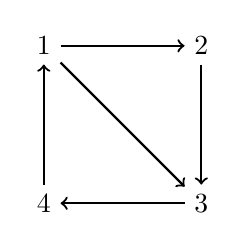
\begin{tikzpicture}
\node (atom1) at (0,2) {1};
\node (atom2) at (2,2) {2};
\node (atom3) at (2,0) {3};
\node (atom4) at (0,0) {4};
\draw[->, thick] (atom1)--(atom2);
\draw[->, thick] (atom2)--(atom3);
\draw[->, thick] (atom3)--(atom4);
\draw[->, thick] (atom4)--(atom1);
\draw[->, thick] (atom1) -- (atom3);
\end{tikzpicture}
\end{center}
Este diagrama é adequado para caracterizar uma interpretação cujo domínio são os números de $1$ a $4$ e que tem uma única relação binária `$\atom{R}{x,y}$', que é verdadeira dos seguintes pares:
	\begin{center}
		\ntuple{1, 2}, 
		\ntuple{2, 3}, 
		\ntuple{3, 4}, 
		\ntuple{4, 1}, 
		\ntuple{1, 3}
	\end{center}
Da mesma forma, podemos oferecer:

\begin{center}
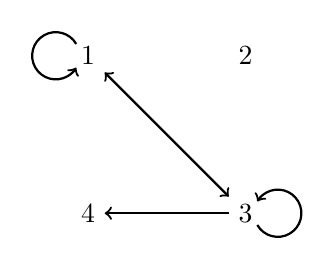
\begin{tikzpicture}
\node (atom1) at (0,2) {1};
\node (atom2) at (2,2) {2};
\node (atom3) at (2,0) {3};
\node (atom4) at (0,0) {4};
\draw[->, thick] (atom3)--(atom4);
\draw[->, thick] (atom1)+(-0.15,0.15) arc (-330:-30:.3); 
\draw[->, thick] (atom3)+(0.15,-0.15) arc (-150:150:.3); 
\draw[<->, thick] (atom1) -- (atom3);
\end{tikzpicture}
\end{center}
para uma interpretação com o mesmo domínio, e com uma relação binária `$\atom{R}{x,y}$' cuja extensão é dada pelos seguintes pares:
	\begin{center}
		\ntuple{1, 3}, 
		\ntuple{3, 1}, 
		\ntuple{3, 4}, 
		\ntuple{1, 1},
		\ntuple{3, 3}
	\end{center}
Se quisermos, podemos tornar nossos diagramas mais complexos. Por exemplo, podemos adicionar nomes como rótulos para objetos específicos.
Da mesma forma, para simbolizar a extensão de um predicado de um lugar, podemos simplesmente desenhar um anel em torno de alguns objetos específicos e estipular que os objetos assim circundados (e somente eles) satisfazem o predicado em questão. 


\chapter{A verdade na LPO}\label{s:TruthFOL}
Não custa nada relembrar aqui que o objetivo principal do estudo da lógica é avaliar argumentos, separando os válidos dos inválidos.
E também não custa nada relembrar que um argumento é válido quando suas premissas justificam sua conclusão, ou seja, quando não é possível haver uma situação em que suas premissas sejam todas verdadeiras, mas sua conclusão seja falsa.
Então, antes de sermos capazes de avaliar argumentos na LPO, precisamos ser capazes de ligar as sentenças da LPO a situações em que poderemos avaliar se elas são verdadeiras ou falsas.

%Na LVF, esta ponte entre as sentenças simbolizadas e as situações é feita pelas valorações.
Na LVF, esta ponte que nos possibilita interpretar sentenças simbolizadas em situações nas quais elas serão verdadeiras ou falsas é dada pelas chaves de simbolização, juntamente com as valorações.
%Através de uma chave de simbolização, situações distintas produzem valorações distintas nas quais as sentenças são verdadeiras ou falsas;
Através de uma chave de simbolização, a verdade ou falsidade das sentenças em português nas diversas situações transforma-se na verdade ou falsidade das sentenças simbolizadas na LVF nas diversas valorações.
Uma chave de simbolização liga situações distintas a valorações distintas que correspondem às diversas linhas das tabelas de verdade, nas quais as sentenças da LPO são verdadeiras ou falsas.
E a consideração dos valores de verdade das sentenças em todas as valorações possíveis, feita nas tabelas de verdade, nos possibilita avaliar a validade dos argumentos.\footnote{
	Se quiser relembrar os detalhes deste processo na LVF, releia a Seção~\ref{s:SustentValid}, p.\,\pageref{s:SustentValid}.}
%e a consideração, através das tabelas de verdade, de todas as valorações possíveis, nos possibilita avaliar a validade dos argumentos.

No caso da LPO, esta ponte entre as sentenças simbolizadas e as situações é feita pela noção de interpretação, introduzida na Seção \ref{s:Interpret}, p.\,\pageref{s:Interpret}.
Vimos ali que uma interpretação é uma chave de simbolização composta por: 
\begin{ebullet}
	\item um domínio do discurso;
	\item uma atribuição (direta ou indireta) de valores de verdade para cada letra sentencial;
	\item a definição de uma referência, no domínio, para cada nome;
	\item a definição (dierta ou indireta) de uma extensão para cada predicado e relação.
\end{ebullet}
Uma chave de simbolização com todos esses componentes constitui uma interpretação e nos fornece tudo o que precisamos para decidir se uma sentença qualquer da LPO é verdadeira ou falsa.
Entender como utilizar interpretações para classificar as sentenças da LPO como verdadeiras ou falsas é o primeiro passo para conseguirmos avaliar argumentos na LPO, e será nossa tarefa neste capítulo.

Sabemos, do Capítulo \ref{s:FOLSentences}, que existem três tipos de sentenças na LPO:
	\begin{itemize}
		\item sentenças atômicas:
		\begin{ebullet}
			\item $\atom{C}{b}$
			\item $\atom{A}{r,j}$
			\item $Q$
		\end{ebullet}
		\item sentenças cujo operador principal é um conectivo sentencial:
		\begin{ebullet}
			\item $\atom{C}{b} \eand Q$
			\item $\atom{A}{r,j} \eif \forall x\,\atom{C}{x}$
			\item $\enot Q$
		\end{ebullet}
		\item sentenças cujo operador principal é um quantificador:
		\begin{ebullet}
			\item $\exists x\,\atom{C}{x}$
			\item $\forall x (\atom{A}{x,j} \eif \atom{C}{x})$
			\item $\exists x \exists y (\atom{A}{x,y} \eand \atom{A}{y,x})$
		\end{ebullet}
	\end{itemize}
Temos que explicar como atribuir valores de verdade para cada um destes tipos de sentenças.

A explicação que daremos aqui é completamente geral e vale para qualquer interpretação.
No entanto, para facilitar a compreensão, usaremos a seguinte interpretação como exemplo privilegiado:
\begin{center}\label{i:Sample}
	\begin{ekey}
		\item[\text{domínio}] {\small todas as pessoas (vivas ou mortas) nascidas antes do ano 2020}
		\item[a] {\small Aristóteles}
		\item[b] {\small Simona Talma}
		\item[C] {\small Simona Talma é uma artista potiguar\,}\footnote{
			Poderíamos aqui ter criado um predicado tal como `$\atom{P}{x}$' para `\gap{x}~é uma artista portiguar' e simbolizar `Simona Talma é uma artista potiguar' como `$\atom{P}{b}$'.
			Não fizemos isso porque queremos que a interpretação de nosso exemplo tenha também uma letra sentencial `$C$' que, tal  como na LVF, tem exatamente o mesmo valor de verdade que a sentença `Simona Talma é uma artista potiguar'.}
		\item[D] {\small é F (uma sentença falsa)}\footnote{
			Aqui estamos apenas indicando diretamente, sem nenhuma sentença em português intermediária, que a letra sentencial `$D$' é uma sentença falsa.}
		\item[\atom{F}{x}] \gap{x} {\small é filósofo}
		\item[\atom{R}{x,y}] \gap{x} {\small nasceu antes que} \gap{y}
	\end{ekey}
\end{center}
Esta interpretação será o nosso caso de estudo nas Seções seguintes.


\section{Sentenças atômicas}
Existem três tipos de sentenças atômicas na LPO, as letras sentenciais, tais como `$C$' e `$D$', os predicados seguidos de nomes, tais como  `$\atom{F}{a}$' e `$\atom{F}{b}$', e as relações $n$-árias seguidas de $n$-uplas ordenadas de nomes, tais como `$\atom{R}{a,b}$' e `$\atom{R}{b,a}$'.
Precisamos, então, entender como as interpretações atribuem valores de verdade para cada um desses três tipos de sentenças atômicas.

No caso das letras sentenciais, isso é uma operação imediata idêntica ao que fazíamos na LVF.
A interpretação estabelece direta ou indiretamente se a letra sentencial é verdadeira ou falsa.
Em nosso exemplo
\begin{center}
	$`C'$ \ \ é \ \ verdadeira   
\end{center}
porque Simona Talma é mesmo uma artista potiguar.
A interpretação nos dá aqui uma especificação indireta através da sentença em português `Simona Talma é uma artista potiguar'.
A letra sentencial terá o mesmo valor de verdade desta sentença.

Por outro lado,
\begin{center}
	$`D'$ \ \ é \ \ falsa   
\end{center}
porque a interpretação estabelece diretamente este fato, sem qualquer sentença intermediária.

%Se a sentença atômica for constituída por um predicado seguido de um nome, tal como `$\atom{F}{a}$', ela será verdadeira apenas no caso do predicado `$\atom{F}{x}$' ser verdadeiro do indivíduo que `$a$' nomeia.
Quando a sentença atômica é constituída por um predicado seguido de um nome, tal como `$\atom{F}{a}$', ela será verdadeira apenas no caso em que o indivíduo que `$a$' nomeia esteja na extensão do predicado `$\atom{F}{x}$'.
Em nossa interpretação, a extensão de `$\atom{F}{x}$' é dada indiretamente pelo predicado `\gap{x} é filósofo'.
Então,
\begin{center}
	`$\atom{F}{a}$' \ \ é \ \ verdadeira
\end{center}
já que `$a$' nomeia Aristóteles e Aristóteles é um filósofo.
De modo semelhante,
\begin{center}
	`$\atom{F}{b}$' \ \ é \ \ falsa
\end{center}
porque `$b$' nomeia Simona Talma, que não é uma filósofa.

Por fim, se a sentença atômica for uma relação seguida de uma sequência ordenada de nomes, tal como `$\atom{R}{a,b}$', ela será verdadeira apenas se o par ordenado dos indivíduos nomeados por `$a$' e `$b$', \ntuple{Aristóteles, Simona Talma}, estiver na extensão do predicado `$\atom{R}{x,y}$'.
Em nossa interpretação esta extensão é definida indiretamente através da relação
\begin{center}
	`\gap{x} nasceu antes que \gap{y}'.
\end{center}	
Como Aristóteles nasceu antes de Simona Talma, então o par \ntuple{Aristóteles, Simona Talma} está na extensão de `$\atom{R}{x,y}$' e
\begin{center}
	`$\atom{R}{a,b}$' \ \ é \ \ verdadeira
\end{center}
Da mesma forma, podemos facilmente verificar que 
\begin{center}
	`$\atom{R}{a,a}$' \ \ é \ \ falsa
\end{center}
porque Aristóteles não nasceu antes que Aristóteles.

Lidar com sentenças atômicas é, portanto, muito intuitivo.
As letras sentencias são tratadas exatamente do mesmo modo que na LVF e quando \meta{R} é um predicado $n$-lugares e \mbox{$\meta{a}_1 $, $\meta{a}_{2}$, \dots, $\meta{a}_{n}$} \ são nomes, temos:

	\factoidbox{
		$\atom{\meta{R}}{\meta{a}_{1},\meta{a}_{2},\dots,\meta{a}_{n}}$ é verdadeira em uma interpretação\\
		\textbf{se e somente se}\\
		$\meta{R}$ é verdadeira dos objetos nomeados por $\meta{a}_{1}$, $\meta{a}_{2}$, \dots, $\meta{a}_{n}$ na interpretação (considerados nesta ordem)
	}
Lembre-se, porém, de que existe um tipo especial de sentença atômica: dois nomes conectados por um sinal de identidade constituem uma sentença atômica.
Esse tipo de sentença atômica também é fácil de lidar.
Sejam \meta{a} e \meta{b} nomes quaisquer,
	\factoidbox{
		$\meta{a} = \meta{b}$ é verdadeira em uma interpretação\\
		\textbf{se e somente se}\\
		 \meta{a} e \meta{b} são nomes do mesmo objeto nesta interpretação
	}
Portanto, em nossa interpretação,
\begin{center}
	`$a=b$' \ \ é \ \ falsa
\end{center}
porque Aristóteles e Simona Talma não são a mesma pessoa.


\section{Conectivos sentenciais}
Vimos no Capítulo \ref{s:FOLSentences} que as sentenças da LPO podem ser criadas a partir de sentenças mais simples, usando os conectivos verofuncionais da LVF. As regras que governam a atribuição de verdade ou falsidade a sentenças deste tipo na LPO são \emph{exatamente} as mesmas da LVF.
Aqui estão elas:
	\factoidbox{
		$\meta{A} \eand \meta{B}$ é verdadeira em uma interpretação\\ \textbf{se e somente se}\\
		$\meta{A}$ e $\meta{B}$ são ambas verdadeiras nesta interpretação
		
		\bigskip
		$\meta{A} \eor \meta{B}$ é verdadeira em uma interpretação\\  \textbf{se e somente se}\\
		$\meta{A}$ é verdadeira ou $\meta{B}$ é verdadeira nesta interpretação

		\bigskip
		$\enot \meta{A}$ é verdadeira em uma interpretação\\ \textbf{se e somente se}\\
		$\meta{A}$ é falsa nesta interpretação

		\bigskip
		$\meta{A} \eif \meta{B}$ é verdadeira em uma interpretação\\ \textbf{se e somente se}\\
		$\meta{A}$ é falsa ou $\meta{B}$ é verdadeira nesta interpretação

		\bigskip
		$\meta{A} \eiff \meta{B}$ é verdadeira em uma interpretação\\ \textbf{se e somente se}\\
		$\meta{A}$ e $\meta{B}$ têm o mesmo valor de verdade nesta interpretação
	}\label{b:ConSent}
Estas definições nos dão, de um modo diferente, exatamente a mesma informação que as tabelas de verdade características dos conectivos, que vimos no Capítulo \ref{s:CharacteristicTruthTables}, p.\,\pageref{s:CharacteristicTruthTables}.
Alguns exemplos nos ajudarão aqui.
A ideia é aplicar as definições do quadro acima à nossa interpretação exemplo (p.\,\pageref{i:Sample}) para decidir o valor de verdade das sentenças:
	\begin{earg}
		\item[\textbullet] `$a = a \eand \atom{F}{a}$' \ \ é \ \ verdadeira\\
			porque tanto `$a = a$' quanto `$\atom{F}{a}$' são verdadeiras
		\item[\textbullet] `$\atom{R}{a,b} \eand \atom{F}{b}$' \ \ é \ \ falsa\\
			porque ainda que `$\atom{R}{a,b}$' seja verdadeira, `$\atom{F}{b}$' é falsa\\
		\item[\textbullet] `$a = b \eor \atom{F}{a}$' \ \ é \ \ verdadeira\\
			porque ainda que  `$a = b$' seja falsa, `$\atom{F}{a}$' é verdadeira\\
		\item[\textbullet] `$\enot a = b$' \ \ é \ \ verdadeira\\
			porque `$a = b$' é falsa\\
		\item[\textbullet] `$\atom{F}{a} \eand \enot( a= b \eand \atom{R}{a,b})$' \ \ é \ \ verdadeira\\
			porque `$\atom{F}{a}$' é verdadeira e `$a = b$' é falsa
	\end{earg}
Antes de prosseguir, certifique-se de ter compreendido todos esses exemplos.
Simplesmente aplicamos, em cada caso, a definição correspondente do quadro acima (p.\,\pageref{b:ConSent}). 


\section[Quantificadores]{Quando o operador principal é um quantificador}\label{s:MainLogicalOperatorQuantifier}
Até aqui viemos bem, mas ainda não tratamos do aspecto que representa a principal novidade introduzida na LPO:
as sentenças cujo operador principal é um \emph{quantificador}.
Veremos que expressar as condições de verdade deste tipo de sentenças é um pouco mais complicado do que parece à primeira vista.
A ideia geral até que é simples e já foi mencionada de passagem em capítulos anteriores:
	\begin{earg}
		\item[\textbullet] $\forall x \atom{\meta{A}}{x}$ é verdadeira \ \ \textbf{se e somente se}\\
		$\atom{\meta{A}}{x}$ for verdadeira \textit{de todos} os elementos do domínio.\\
		\item[\textbullet] $\exists x \atom{\meta{B}}{x}$ é verdadeira \ \ \textbf{se e somente se}\\
		$\atom{\meta{B}}{x}$ for verdadeira \textit{de algum} elemento do domínio.
	\end{earg}
A dificuldade maior não é esta ideia geral, mas a especificação de sua definição precisa.

Vamos aqui nos aproximar pouco a pouco da definição.
Começaremos com algumas propostas ingênuas e vamos corrigindo-as até, eventualmente, chegarmos à definição correta.
Uma primeira proposta é a seguinte:
se, como vimos, `$\forall x\,\atom{F}{x}$' deve ser verdadeira se e somente se `$\atom{F}{x}$' é verdadeira para tudo no domínio,
então poderíamos simplesmente considerar que uma sentença universal é verdadeira quando a extensão do predicado que a segue compreende todo o domínio do discurso.

Esta ideia funciona quando o que vem após o quantificador inicial é um predicado, como em  `$\forall x\,\atom{F}{x}$'.
Mas, infelizmente, essa ideia não é geral o suficiente para especificar as condições de verdade de sentenças onde o que segue o quantificador inicial não é um predicado, mas outra expressão quantificada, tal como ocorre em:
$$\forall x \exists y\,\atom{L}{x,y}$$
Não conseguimos aplicar esta ideia aqui, porque o que segue o quantificador não é um predicado, mas a expressão quantificada `$\exists y\,\atom{L}{x,y}$'.
E as interpretações não têm cláusulas que indicam se `$\exists y\,\atom{L}{x,y}$' é verdadeira de tudo no domínio.
As cláusulas das intepretações especificam apenas a referência de nomes e a extensão de predicados e relações.

Para tentar corrigir isso poderíamos então sugerir que `$\forall x \exists y\, \atom{L}{x,y}$' deve ser verdadeira em uma interpretação se e somente se $\exists y\, \atom{L}{\meta{a},y}$ for verdadeira para \emph{todo} nome \meta{a} da interpretação.
E, de modo similar, diríamos que $\exists y\, \atom{L}{\meta{a},y}$ é verdadeira se e somente se $\atom{L}{\meta{a}, \meta{b}}$ for verdadeira para \emph{algum} nome \meta{b}.
Então, juntando estes dois passos, `$\forall x \exists y\, \atom{L}{x,y}$' seria verdadeira em uma interpretação se e somente se $\atom{L}{\meta{a}, \meta{b}}$ for verdadeira para \emph{todo} nome \meta{a} e \emph{algum} nome \meta{b} presentes na interpretação.

Infelizmente, isso também não funciona.
Para entender por que, basta observar que na interpretação de nossos exemplos (p.\,\pageref{i:Sample}), apenas duas pessoas têm nome, mas o domínio comporta todas as pessoas nascidas antes do ano 2020.

Uma terceira ideia, então, é a seguinte.
Mesmo que uma interpretação não tenha nomes para \emph{todos} os indivíduos do domínio, ela poderia ter.
Ou seja, podemos estender uma interpretação qualquer, de modo a que todos os elementos do domínio tenham nomes.
Antes de prosseguir com a definição, vejamos alguns exemplos de como isso pode funcionar.

Em nossa interpretação privilegiada (p.\,\pageref{i:Sample}) `$\exists x\, \atom{R}{b,x}$' deve ser verdadeira. Afinal, certamente há no domínio alguém que nasceu depois que Simona Talma.
Dani Cruz (uma outra artista potiguar) é uma dessas pessoas.
De fato, se estendermos temporariamente nossa interpretação adicionando o nome `$c$' para se referir a Dani Cruz, então `$\atom{R}{b,c}$' será verdadeira nessa interpretação estendida.
E este fato certamente deve ser suficiente para assegurar que `$\exists x\,\atom{R}{b,x}$' é verdadeira na nossa interpretação original, já que ele indica que há pelo menos uma pessoa no domínio (Dani Cruz) que nasceu depois de Simona Talma.

Na nossa interpretação, `$\exists x (\atom{F}{x} \eand \atom{R}{x,a})$' também deve ser verdadeira.
Afinal, no domínio, certamente há alguém que foi filósofo e nasceu antes de Aristóteles.
Sócrates é uma dessas pessoas.
De fato, se estendermos nossa interpretação, com um novo nome, `$d$', que denota Sócrates, então `$\atom{F}{d} \eand \atom{R}{d,a}$' será verdadeira nessa interpretação estendida.
Novamente, isso certamente é suficiente como garantia de que `$\exists x (\atom{F}{x} \eand \atom{R}{x,a})$' é verdadeira na interpretação original (não estendida), já que isso indica que há pelo menos uma pessoa no domínio (Sócrates) que é filósofo e nasceu antes de Aristóteles.

Já a sentença `$\forall x \exists y\, \atom{R}{x,y}$' deve ser falsa em nossa interpretação.
Afinal, certamente há uma última pessoa que nasceu antes do ano 2020 começar.
Não sabemos quem é esta pessoa, mas podemos, mesmo assim, estender a interpretação para que um nome novo, `$e$', denote exatamente esta pessoa.
E fazendo isso, qualquer que seja o indivíduo do domínio ao qual um outro nome novo $`f'$ se refira, a sentença `$\atom{R}{e,f}$' seria falsa.
De fato, não importa \emph{quem} seja a referência do nome `$f$', sabemos que `$\atom{R}{e,f}$' será falsa, já que `$e$' denota a última pessoa nascida em 2019. 
Esse fato é certamente suficiente para garantir que `$\exists y\, \atom{R}{e,y}$' é falsa na interpretação estendida. E isso, por sua vez, é certamente suficiente como garantia de que `$\forall x \exists y\, \atom{R}{x,y}$' é falsa na nossa interpretação original.

Se você entendeu esses três exemplos, ótimo. É isso que importa.
O que temos que fazer, agora, é fornecer uma definição precisa dessas ideias, que exprima as condições de verdade para sentenças quantificadas.
Para isso precisamos de mais notação em nossa metalinguagem.
A expressão:
$$\meta{A}(\meta{x})$$
será usada para denotar na metalinguagem uma fórmula que contenha pelo menos uma ocorrência livre da variável \meta{x}.
Ou seja, há uma ou mais ocorrências de \meta{x} em \meta{A} que estão fora do escopo de qualquer `$\forall x$' e `$\exists x$' em \meta{A}.
Seja \meta{c} um nome.
A expressão:
$$\meta{A}(\meta{c})$$
será usada para denotar na metalinguagem a fórmula obtida quando substituímos por $\meta{c}$ \emph{todas} as ocorrências livres de $\meta{x}$ em \meta{A}.
A fórmula resultante, $\meta{A}(\meta{c})$, é chamada de \define{substitution instance} de $\forall \meta{x} \meta{A}$ e $\exists \meta{x} \meta{A}$.
Além disso, $\meta{c}$ é chamado de \xdefine{nome de instanciacao}.

Vejamos um exemplo.
Considere a sentença da LPO:
	$$\forall y \exists x (\atom{R}{y,x} \eiff \atom{F}{x})$$
A notação recém  introduzida nos permite usar a expressão
	$$\forall \meta{y} \atom{\meta{A}}{\meta{y}}$$
para nos referirmos a esta sentença de um modo genérico em nossa metalinguagem.
Quando fazemos isso, a expressão
	$$\atom{\meta{A}}{\meta{y}}$$
refere-se genericamente a
	$$\exists x (\atom{R}{y,x} \eiff \atom{F}{x})$$
que é uma fórmula com uma ocorrência livre da variável `$y$'.
Se substituímos esta ocorrência livre de `$y$' por um nome, digamos, `$e$', obtemos a sentença:
	$$\exists x (\atom{R}{e,x} \eiff \atom{F}{x})$$
Esta sentença nada mais é do que uma instância de substituição de 
	$$\forall y \exists x (\atom{R}{y,x} \eiff \atom{F}{x})$$
onde `$e$' é o nome de instanciação, e `$y$' é a variável instanciada.

Seja $\mathbf{I}$ o nome de uma interpretação que estejamos considerando.
$\mathbf{I}$ inclui uma especificação de quais nomes correspondem a quais objetos no domínio.
Considere um objeto  qualquer do domínio, digamos, $d$, e um nome $\meta{c}$ que não esteja sendo usado em $\mathbf{I}$.
Usaremos a notação
$$\mathbf{I}[d/\meta{c}]$$
para nos referirmos à interpretação que é igual a $\mathbf{I}$, com um acréscimo:
$\mathbf{I}[d/\meta{c}]$ atribui o nome $\meta{c}$ ao objeto $d$.
Então podemos dizer que $d$ \xdefine{satisfaz} a fórmula $\meta{A}(\meta{x})$ na interpretação $\mathbf{I}$ se e somente se $\meta{A}(\meta{c})$ é verdadeira em $\mathbf{I}[d/\meta{c}]$.
(Quando $d$ satisfaz $\meta{A}(\meta{x})$, nós dizemos também que $\meta{A}(\meta{x})$ é \emph{verdadeira de} $d$.

\factoidbox{A interpretação $\mathbf{I}[d/\meta{c}]$ é igual à interpretação $\mathbf{I}$, com o acréscimo de que atribui o nome $\meta{c}$ ao objeto $d$.

\
\\
Um objeto $d$ \xdefine{satisfaz} $\meta{A}(\meta{x})$ na interpretação $\mathbf{I}$ \\
\hbox{\textbf{se e somente se}} $\meta{A}(\meta{c})$ é verdadeira em $\mathbf{I}[d/\meta{c}]$.
}

\noindent Assim, por exemplo, dizemos que: 
\begin{ebullet}
	\item Sócrates \underline{satisfaz} a fórmula `$\atom{F}{x}$'
\end{ebullet}
pois:
\begin{ebullet}
	\item $\atom{F}{c}$ é \underline{verdadeira} na interpretação $\mathbf{I}[\text{Sócrates}/c]$
\end{ebullet}
ou seja, $\atom{F}{c}$ é verdadeira na interpretação que obtemos de nossa interpretação original $\mathbf{I}$ (p.\pageref{i:Sample}) quando acrescentamos a indicação de que o nome `$c$' se refere a Sócrates:

\begin{center}
	\begin{ekey}
		\item[\text{domínio}] {\small todas as pessoas (vivas ou mortas) nascidas antes do ano 2020}
		\item[a] {\small Aristóteles}
		\item[b] {\small Simona Talma}
		\item[c] {\small Sócrates}
		\item[C] {\small Simona Talma é uma artista potiguar\,}
		\item[D] {\small é F (uma sentença falsa)}
		\item[\atom{F}{x}] \gap{x} {\small é filósofo}
		\item[\atom{R}{x,y}] \gap{x} {\small nasceu antes que} \gap{y}
	\end{ekey}
\end{center}

Tendo ampliado nossa metalinguagem com estas notações, podemos finalmente definir as condições de verdade de sentenças da LPO cujo operador principal é um quantificador.
A ideia aproximada é a seguinte.
A sentença $\forall \meta{x}\meta{A}(\meta{x})$ será verdadeira em $\mathbf{I}$ se e somente se, para qualquer objeto $d$ no domínio, $\meta{A}(\meta{c})$ é verdadeira em $\mathbf{I}[d/\meta{c}]$.
Ou seja, $\forall \meta{x}\meta{A}(\meta{x})$ será verdadeira  se e somente se $\meta{A}(\meta{c})$ for verdadeira, independentemente de qual objeto (no domínio) tenha sido nomeado  por $\meta{c}$.
Em outras palavras, $\forall \meta{x} \meta{A}(\meta{x})$ é verdadeira apenas quando todos os objetos no domínio satisfazem $\meta{A}(\meta{x})$.

Similarmente, a sentença $\exists \meta{x}\meta{A}(\meta{x})$ será verdadeira se e somente se houver \emph{algum} objeto no domínio que satisfaça $\meta{A}(\meta{x})$.
Ou seja, $\exists \meta{x}\meta{A}(\meta{x})$ é verdadeira em $\mathbf{I}$ se e somente se  $\meta{A}(\meta{c})$ é verdadeira em $\mathbf{I}[d/\meta{c}]$ para pelo menos um objeto $d$.
	\factoidbox{
		$\forall \meta{x}\meta{A}(\meta{x})$ é \underline{verdadeira} em uma interpretação \textbf{se e somente se} todo objeto no domínio \underline{satisfiaz} $\meta{A}(\meta{x})$.
		
		\
		\\
		$\exists \meta{x}\meta{A}(\meta{x})$ é \underline{verdadeira} em uma interpretação \textbf{se e somente se} pelo menos um objeto no domínio \underline{satisfaz} $\meta{A}(\meta{x})$.
	}
Para ficar claro: tudo o que estamos fazendo aqui é formalizar (de um modo bastante preciso) a ideia intuitiva de que para que uma sentença quantifidada universalmente seja verdadeira, todos os objetos do domínio precisam satisfazê-la; e para que uma sentença quantificada existencialmente seja verdadeira, basta que um objeto do domínio a satisfaça. 

Finalmente, vale notar que o conceito de um objeto satisfazer uma fórmula com uma variável livre também pode ser estendido a fórmulas com mais de uma variável livre.
Por exemplo, se tivermos uma fórmula $\meta{A}(\meta{x},\meta{y})$ com duas variáveis livres $\meta{x}$ e $\meta{y}$, podemos dizer que um par de objetos $\langle a, b\rangle$ satisfaz $\meta{A}(\meta{x},\meta{y})$ se e somente se $\meta{A}(\meta{c},\meta{d})$ for verdadeira na interpretação estendida por dois nomes $\meta{c}$ e $\meta{d}$, onde $\meta{c}$ é o nome de $a$ e $\meta{d}$ é o nome de $b$.
Assim, por exemplo, $\langle \text{Sócrates}, \text{Platão}\rangle$ satisfaz $R(x,y)$, pois, já que Sócrates nasceu antes de Platão, $R(c,d)$ é verdadeiro na interpretação:
\begin{center}
	\begin{ekey}
		\item[\text{domínio}] {\footnotesize todas as pessoas (vivas ou mortas) nascidas antes do ano 2020}
		\item[a] {\small Aristóteles}
		\item[b] {\small Simona Talma}
		\item[c] {\small Sócrates}
		\item[d] {\small Platão}
		\item[C] {\small Simona Talma é uma artista potiguar\,}
		\item[D] {\small é F (uma sentença falsa)}
		\item[\atom{F}{x}] \gap{x} {\small é filósofo}
		\item[\atom{R}{x,y}] \gap{x} {\small nasceu antes que} \gap{y}
	\end{ekey}
\end{center}
Para fórmulas atômicas, tais como $\atom{F}{x}$ e $\atom{R}{x,y}$,  os objetos ou sequências de objetos que as satisfazem são exatamente a extensão dos predicados que as constituem.
Mas a noção de satisfação também se aplica a fórmulas não atômicas.
A fórmula $\atom{F}{x} \land \atom{R}{x,b}$, por exemplo, é satisfeita por todos os filósofos que nasceram antes de Simona Talma.
A ideia de satisfação aplica-se até mesmo a fórmulas envolvendo quantificadores.
Por exemplo, $F(x) \eand \lnot\exists y(F(y) \land R(y,x))$ é satisfeita por todos os filósofos para os quais nenhum filósofo nasceu antes deles---em outras palavras, o primeiro filósofo, e apenas ele, satisfaz esta fórmula.


\practiceproblems
\solutions
\problempart
\label{pr.TorF1}
Considere a seguinte interpretação:
	\begin{ebullet}\small
		\item O domínio compreende apenas Benedita e Clayton
		\item `$\atom{A}{x}$' é verdadeira para ambos, tanto Benedita quanto Clayton
		\item `$\atom{B}{x}$' é verdadeira apenas para Benedita
		\item `$\atom{N}{x}$' não é verdadeira nem para Benedita nem para Clayton
		\item `$c$' refere-se a Clayton
	\end{ebullet}
Para cada uma das nove sentenças seguintes, determine se ela é verdadeira ou falsa nesta interpretação.
\begin{earg}
\item $\atom{B}{c} $
\item $\atom{A}{c}  \eiff \enot \atom{N}{c}$
\item $\atom{N}{c}  \eif (\atom{A}{c} \eor \atom{B}{c})$
\item $\forall x\, \atom{A}{x}$
\item $\forall x \enot \atom{B}{x}$
\item $\exists x(\atom{A}{x} \eand \atom{B}{x})$
\item $\exists x(\atom{A}{x} \eif \atom{N}{x})$
\item $\forall x(\atom{N}{x} \eor \enot \atom{N}{x})$
\item $\exists x\, \atom{B}{x} \eif \forall x\, \atom{A}{x}$
\end{earg}

\problempart
\label{pr.TorF2}
Considere a seguinte interpretação:	
	\begin{ebullet}
		\item O domínio compreende apenas Leila, Cora e Ênio
		\item `$\atom{G}{x}$' é verdadeira de Leila, de Cora e de Ênio
		\item `$\atom{H}{x}$' é verdadeira apenas de Cora
		\item `$\atom{M}{x}$' é verdadeira apenas de Leila e Ênio
		\item `$c$' refere-se a Cora
		\item `$e$' refere-se a Ênio
	\end{ebullet}
Para cada uma das quinze sentenças seguintes, determine se ela é verdadeira ou falsa nesta interpretação.
\begin{earg}
\item $\atom{H}{c} $
\item $\atom{H}{e} $
\item $\atom{M}{c}  \eor \atom{M}{e}$
\item $\atom{G}{c}  \eor \enot \atom{G}{c}$
\item $\atom{M}{c}  \eif \atom{G}{c}$
\item $\exists x\, \atom{H}{x}$
\item $\forall x\, \atom{H}{x}$
\item $\exists x\, \enot \atom{M}{x}$
\item $\exists x(\atom{H}{x} \eand \atom{G}{x})$
\item $\exists x(\atom{M}{x} \eand \atom{G}{x})$
\item $\forall x(\atom{H}{x} \eor \atom{M}{x})$
\item $\exists x\, \atom{H}{x} \eand \exists x\, \atom{M}{x}$
\item $\forall x(\atom{H}{x} \eiff \enot \atom{M}{x})$
\item $\exists x\, \atom{G}{x} \eand \exists x \enot \atom{G}{x}$
\item $\forall x\exists y(\atom{G}{x} \eand \atom{H}{y})$
\end{earg}

\problempart
\label{pr.TorF3}
Conforme as convenções introduzidas no final do Capítulo~\ref{s:Interpretations} (p.\,\pageref{s:Interpret}), o diagrama abaixo especifica uma interpretação cujo domínio é o conjunto $\{1,2,3,4,5\}$ e que tem uma única relação binária $\atom{R}{x,y}$, cuja extensão é dada pelas setas do diagrama:
\begin{center}
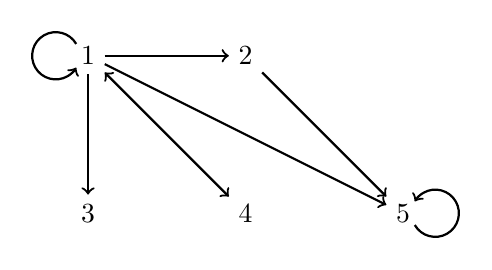
\begin{tikzpicture}
\node (atom1) at (0,2) {1};
\node (atom2) at (2,2) {2};
\node (atom4) at (0,0) {3};
\node (atom5) at (2,0) {4};
\node (atom6) at (4,0) {5};
\draw[->, thick] (atom1)+(-0.15,0.15) arc (-330:-30:.3); 
\draw[->, thick] (atom6)+(0.15,-0.15) arc (-150:150:.3); 
\draw[->, thick] (atom1) -- (atom2);
\draw[->, thick] (atom1) -- (atom4);
\draw[<->, thick] (atom1) -- (atom5);
\draw[->, thick] (atom1) -- (atom6);
\draw[->, thick] (atom2) -- (atom6);
\end{tikzpicture}
\end{center}
Para cada uma das doze sentenças seguintes, determine se ela é verdadeira ou falsa nesta interpretação.
\begin{earg}
\item $\exists x\, \atom{R}{x,x}$
\item $\forall x\, \atom{R}{x,x}$
\item $\exists x \forall y\, \atom{R}{x,y}$
\item $\exists x \forall y\, \atom{R}{y,x}$
\item $\forall x \forall y \forall z ((\atom{R}{x,y} \eand \atom{R}{y,z}) \eif \atom{R}{x,z})$
\item $\forall x \forall y \forall z ((\atom{R}{x,y} \eand \atom{R}{x,z}) \eif \atom{R}{y,z})$
\item $\exists x \forall y\, \enot \atom{R}{x,y}$
\item $\forall x(\exists y\, \atom{R}{x,y} \eif \exists y\, \atom{R}{y,x})$
\item $\exists x \exists y (\enot x = y \eand \atom{R}{x,y} \eand \atom{R}{y,x})$
\item $\exists x \forall y(\atom{R}{x,y} \eiff x = y)$
\item $\exists x \forall y(\atom{R}{y,x} \eiff x = y)$
\item $\exists x \exists y(\enot x = y \eand \atom{R}{x,y} \eand \forall z(\atom{R}{z,x} \eiff y = z))$
\end{earg}


\chapter{Conceitos semânticos}

Oferecer uma definição precisa de sentença verdadeira na LPO foi um pouco complicado, mas agora que terminamos, podemos definir várias noções lógicas importantes.
Elas serão muito parecidas com as definições que oferecemos para a LVF.
No entanto, lembre-se de que agora elas se referem a \emph{interpretações}, e não mais a valorações.

Continuaremos a usar o símbolo `$\entails$' na LPO da mesma forma que o utilizamos na LVF.
Assim:
	$$\meta{A}_1, \meta{A}_2, \ldots, \meta{A}_n \entails\meta{C}$$
significa que não há interpretação na qual $\meta{A}_1$, $\meta{A}_2$, \dots, $\meta{A}_n$ sejam todas verdadeiras e \meta{C} seja falsa. Consequentemente,
	$$\entails\meta{A}$$
significa que \meta{A} é verdadeira em todas as interpretações, ou seja, que é impossível que \meta{A} seja falsa.

As outras noções lógicas que vimos, também têm definições correspondentes na LPO.
Aqui estão elas:

\begin{itemize}
\item Uma sentença  $\meta{A}$ é uma \define{validity} na LPO se e somente se $\meta{A}$ for verdadeira em todas as interpretações; ou seja, se
$$\entails\meta{A}$$
\item $\meta{A}$ é uma \define{contradiction of FOL} na LPO se e somente se $\meta{A}$ for falsa em todas as interpretações; ou seja, se
$$\entails\enot\meta{A}$$
\item $\meta{A}_1, \meta{A}_2, \ldots \meta{A}_n \therefore \meta{C}$ é um argumento \define{valid in FOL} (na LPO) se e somente se não houver interpretação em que todas as premissas são verdadeiras e a conclusão é falsa; ou seja, se
$$\meta{A}_1,\meta{A}_2,\ldots \meta{A}_n \entails\meta{C}$$

\item Um argumento $\meta{A}_1, \meta{A}_2, \ldots \meta{A}_n \therefore \meta{C}$ é \xdefine{invalido na LPO} se e somente se ele não é válido, ou seja, quando há alguma interpretação na qual todas as suas premissas são verdadeiras e a conclusão é falsa.
Denotamos isso por:
$$\meta{A}_1,\meta{A}_2,\ldots \meta{A}_n \nvDash\meta{C}$$
 
\item Duas sentenças da LPO \meta{A} e \meta{B} são \define{equivalent in FOL} se e somente se em toda interpretação na qual uma é verdadeira, a outra também é; ou seja, se
\begin{center}
	$\meta{A}\entails\meta{B}$ \ \ \ e \ \ \ $\meta{B}\entails\meta{A}$
\end{center}

\item As sentenças $\meta{A}_1$, $\meta{A}_2$, \dots, $\meta{A}_n$ são \define{satisfiable in FOL} na LPO se e somente se há alguma interpretação na qual todas são verdadeiras.
Eles são \xdefine{conjuntamente insatisfatorias} se não houver tal interpretação.
\end{itemize}


\chapter{Utilizando as interpretações}
\label{sec.UsingModels}

\section{Validades e contradições}
Suponha que queremos mostrar que
$$\exists x\, \atom{A}{x,x} \eif \atom{B}{d}$$
\emph{não é} uma validade.
Conforme a definição vista no capítulo anterior, temos que mostrar que esta  sentença não é verdadeira em todas as interpretações; isto é, que ela é falsa em alguma interpretação.
Então será suficiente fornecermos uma única interpretação na qual a sentença seja falsa.

Para que `$\exists x\,\atom{A}{x,x} \eif \atom{B}{d}$' seja falsa, o antecedente do condicional (`$\exists x\, \atom{A}{x,x}$') deve ser verdadeiro, e o consequente (`$\atom{B}{d}$') deve ser falso.
Para construir uma interpretação na qual isso ocorra, começamos especificando um domínio.
Manter o domínio pequeno facilita a especificação da extensão dos predicados; portanto, começaremos com um domínio com apenas um indivíduo.
Digamos, então, que o único indivíduo de nosso domínio seja a cidade de Fortaleza.
\begin{center}
	\begin{ekey}
		\item[\text{domínio}] Fortaleza
	\end{ekey}
\end{center}
Nossa sentença tem um nome, `$d$', que precisa nomear algo no domínio.
Então nossa única opção é definir que:
\begin{center}
	\begin{ekey}
		\item[d] Fortaleza
	\end{ekey}
\end{center}
Lembre-se de que queremos que `$\exists x\, \atom{A}{x,x}$' seja verdadeira; portanto, queremos que algum indivíduo do domínio relacione-se consigo mesmo através de `$A$'.
Podemos então propor a seguinte extensão para a relação `$A$':
\begin{center}
	\begin{ekey}
		\item[\atom{A}{x,y}] \gap{x} está no mesmo país que \gap{y}
	\end{ekey}
\end{center}
Agora, `$\atom{A}{d,d}$' é claramente verdadeira, portanto, `$\exists x\, \atom{A}{x,x}$' também é. 
Mas nós também queremos que `$\atom{B}{d}$' seja falsa; portanto, o indivíduo nomeado por `$d$' não deve estar na extensão de `$B$'.
Podemos simplesmente propor que:
\begin{center}
	\begin{ekey}
		\item[\atom{B}{x}] \gap{x} é a capital do Rio Grande do Norte
	\end{ekey}
\end{center}
Construímos uma interpretação em que `$\exists x\, \atom{A}{x,x}$' é verdadeira, mas `$\atom{B}{d}$' é falsa.
Logo, nesta interpretação `$\exists x\, \atom{A}{x,x} \eif \atom{B}{d}$' é falsa e portanto não é uma validade.

Com a mesma facilidade podemos mostrar que `$\exists x\atom{A}{x,x} \eif \atom{B}{d}$' não é uma contradição.
Precisamos apenas especificar uma interpretação na qual `$\exists x\atom{A}{x,x} \eif \atom{B}{d}$' seja verdadeira; ou seja, uma interpretação na qual `$\exists x\, \atom{A}{x,x}$' é falsa ou `$\atom{B}{d}$' é verdadeira.
Aqui está uma:
\begin{center}
	\begin{ekey}
		\item[\text{domínio}] Fortaleza
		\item[d] Fortaleza
		\item[\atom{A}{x,y}] \gap{x} está no mesmo país que \gap{y}
		\item[\atom{B}{x}] \gap{x} é a capital do Ceará
	\end{ekey}
\end{center}
Isso mostra que existe uma interpretação na qual `$\exists x\atom{A}{x,x} \eif \atom{B}{d}$' é verdadeira, e portanto, não é uma contradição.
	\factoidbox{
		Para mostrar que $\meta{A}$ \textbf{não é uma validade}, basta apresentar uma interpretação em que $\meta{A}$ seja falsa.\\
		
		Para mostrar que $\meta{A}$ \textbf{não é uma contradição}, basta apresentar uma interpretação em que $\meta{A}$ seja verdadeira.
	}


\section{Equivalência lógica}
Suponha que queiramos mostrar que
\begin{center}
	$\forall x\, \atom{S}{x}$ \ \ e \ \ $\exists x\, \atom{S}{x}$
\end{center}
\emph{não são} logicamente equivalentes.
Precisamos construir uma interpretação na qual as duas sentenças tenham valores de verdade diferentes.
Queremos que uma das sentenças seja verdadeira e o outra falsa.
Começamos especificando um domínio e, novamente, o menor possível, para facilitar as coisas.
Vamos, no entanto, precisar de pelo menos dois objetos.
(Se o domínio tiver um único objeto as sentenças terão o mesmo valor de verdade. 
Para perceber por que, proponha algumas interpretações com domínios de um único indivíduo e veja o que ocorre com o valor de verdade das duas sentenças.)
Considere, então, o seguinte domínio:
	\begin{center}
	\begin{ekey}
		\item[\text{domínio}] Jackson do Pandeiro, Luiz Gonzaga
	\end{ekey}
	\end{center}
Podemos fazer `$\exists x\, \atom{S}{x}$' ser verdadeira incluindo um dos indivíduos do domínio na extensão de `$S$', e podemos fazer `$\forall x\, \atom{S}{x}$' ser falsa, deixando um dos indivíduos do domínio fora da extensão de `$S$'.
Considere então:
	\begin{center}
	\begin{ekey}
		\item[\atom{S}{x}] \gap{x} toca pandeiro
	\end{ekey}
	\end{center}
Agora `$\exists x\, \atom{S}{x}$' é verdadeira, porque Jackson do Pandeiro satisfaz `$\atom{S}{x}$'.
De modo mais preciso, se estendermos nossa interpretação fazendo `$c$' nomear Jackson do Pandeiro, `$\atom{S}{c}$' torna-se uma sentença verdadeira nessa interpretação estendida.
Portanto, `$\exists x\, \atom{S}{x}$' é verdadeira na interpretação original.
Da mesma forma, `$\forall x\, \atom{S}{x}$' é falsa, porque Luiz Gonzaga não satisfaz `$\atom{S}{x}$'.
Mais precisamente, estender a interpretação fazendo o nome `$d$' se referir a Luiz Gonzaga, torna a sentença `$\atom{S}{d}$' falsa nessa interpretação estendida, já que Luiz Gonzaga não toca pandeiro.
Portanto, `$\forall x\, \atom{S}{x}$' é falso na interpretação original.
Então a interpretação original que propusemos
	\begin{center}
	\begin{ekey}
		\item[\text{domínio}] Jackson do Pandeiro, Luiz Gonzaga
		\item[\atom{S}{x}] \gap{x} toca pandeiro
	\end{ekey}
	\end{center}
comprova que `$\exists x\, \atom{S}{x}$' e `$\forall x\, \atom{S}{x}$' não são logicamente equivalentes, já que a primeira sentença é verdadeira e a segunda é falsa nessa interpretação.
	\factoidbox{
		Para mostrar que $\meta{A}$ e $\meta{B}$ não são logicamente equivalentes, basta encontrar uma interpretação em que uma sentença é verdadeira e a outra é falsa.
	}


\section{Validade, sustentação e satisfação}
Para testar a validade, a sustentação ou a satisfação, normalmente precisamos produzir interpretações capazes de determinam o valor de verdade de várias sentenças.
Considere o seguinte argumento na LPO:
\begin{earg}
	\item[] $\exists x(\atom{G}{x} \eif \atom{G}{a})$
	\item[\therefore ] $\exists x\, \atom{G}{x} \eif \atom{G}{a}$
\end{earg}
%$$\exists x(\atom{G}{x} \eif \atom{G}{a}) \therefore \exists x\, \atom{G}{x} \eif \atom{G}{a}$$
Para mostrar que este argumento é inválido, precisamos encontrar uma interpretação na qual a premissa seja verdadeira, mas a conclusão seja falsa.
A conclusão é um condicional; portanto, ela será falsa quando seu antecedente for verdadeiro e o consequente falso.
Claramente, nosso domínio deve conter dois objetos, um que esteja na extensão de `$G$' e um que não esteja.
Vamos tentar:
	\begin{center}
	\begin{ekey}
		\item[\text{domínio}] Karl Marx, Pelé
		\item[\atom{G}{x}] \gap{x} é co-autor de `O Manifesto Comunista'
		\item[a] Pelé
	\end{ekey}
	\end{center}
Nesta interpretação a sentença `$\atom{G}{a}$' é claramente falsa.
Afinal, Pelé foi o maior jogador de futebol que já houve, e não escreveu nenhum manifesto.
Já Karl Marx é reconhecidamente um dos autores de `O Manifesto Comunista', juntamente com  Friedrich Engels.
Então, `$\exists x\, \atom{G}{x}$' é verdadeira nessa interpretação.
Portanto, como `$\exists x\, \atom{G}{x}$' é verdadeira e `$\atom{G}{a}$' é falsa, a conclusão de nosso argumento, `$\exists x\, \atom{G}{x} \eif \atom{G}{a}$' é uma sentença falsa, conforme requerido.

Será que a premissa é verdadeira?
Sim!
Observe que `$\atom{G}{a} \eif \atom{G}{a}$' é verdadeira. (De fato, `$\atom{G}{a} \eif \atom{G}{a}$' é uma validade, verdadeira em qualquer interpretação)
Então, certamente `$\exists x (\atom{G}{x} \eif \atom{G}{a})$' é verdadeira.
Temos, portanto, uma interpretação na qual a premissa do argumento é verdadeira e a conclusão é falsa.
Logo o argumento é inválido. 

Observe que nossa interpretação mostra também que
\begin{center}
	`$\exists x(\atom{G}{x} \eif \atom{G}{a})$' \ \ \emph{não} sustenta \ \ `$\exists x\, \atom{G}{x} \eif \atom{G}{a}$'
\end{center}
já que nela a primeira sentenças é verdadeira e a segunda é falsa.
Nossa interpretação também mostra que as sentenças abaixo são conjuntamente satisfatórias, já ambas são verdadeiras nela
\begin{center}
	$\exists x (\atom{G}{x} \eif \atom{G}{a})$ \ \ e \ \ $\enot (\exists x\, \atom{G}{x} \eif \atom{G}{a})$
\end{center}

Vejamos mais um exemplo.
Considere:
\begin{earg}
	\item[] $\forall x \exists y\, \atom{L}{x,y}$
	\item[\therefore ] $\exists y \forall x\, \atom{L}{x,y}$
\end{earg}
%$$\forall x \exists y\, \atom{L}{x,y} \therefore \exists y \forall x\, \atom{L}{x,y}$$

Novamente, queremos mostrar que este argumento é inválido.
E fazemos isso propondo uma interpretação onde a premissa é verdadeira, mas a conclusão é falsa.
Aqui está uma sugestão:
	\begin{center}
	\begin{ekey}
		\item[\text{domínio}] todas as pessoas casadas
		\item[\atom{L}{x,y}] \gap{x} é casado(a) com \gap{y}
	\end{ekey}
	\end{center}
A premissa é claramente verdadeira nessa interpretação. Qualquer pessoa no domínio é casada com alguma pessoa, que, por ser casada, também está no domínio.
Logo, `$\forall x \exists y\, \atom{L}{x,y}$' é verdadeira.
Por outro lado, a conclusão, `$\exists y \forall x\, \atom{L}{x,y}$',  é claramente falsa, pois sua verdade exigiria que houvesse uma única pessoa que fosse casada com todas as outras pessoas no domínio, inclusive com ela mesma.
Portanto, o argumento tem premissa verdadeira e conclusão falsa nesta interpretação e, por isso, é inválido.

Como no exemplo anterior, podemos observar ainda, como consequência imediata, que as sentenças `$\forall x \exists y\, \atom{L}{x,y}$' e `$\enot\exists y \forall x\, \atom{L}{x,y}$' são conjuntamente satisfatórias e que `$\forall x \exists y\, \atom{L}{x,y}$' não sustenta `$\exists y \forall x\, \atom{L}{x,y}$'.

Para o nosso terceiro exemplo, vamos misturar as coisas um pouco.
Na Seção \ref{s:Interpret}, p.\,\pageref{s:Interpret}, descrevemos como apresentar algumas interpretações usando diagramas. Por exemplo:
\begin{center}
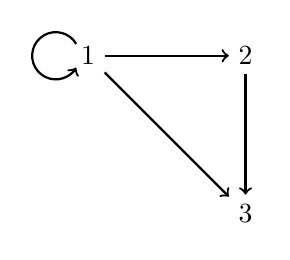
\begin{tikzpicture}
\node (atom1) at (0,2) {1};
\node (atom2) at (2,2) {2};
\node (atom3) at (2,0) {3};
\draw[->, thick] (atom1)--(atom2);
\draw[->, thick] (atom1)--(atom3);
\draw[->, thick] (atom1)+(-0.15,0.15) arc (-330:-30:.3); 
\draw[->, thick] (atom2) -- (atom3);
\end{tikzpicture}
\end{center}
De acordo com as convenções ali apresentadas, o domínio dessa interpretação são os três primeiros números inteiros positivos, e a extensão de  `$\atom{R}{x,y}$' é dada pelas setas do diagrama.
Ou seja, `$\atom{R}{x,y}$' é verdadeira para $\langle x, y \rangle$ apenas caso haja uma seta partindo  de \textbf{x} e chegando em \textbf{y} em nosso diagrama.
Aqui estão algumas sentenças verdadeiras nesta interpretação:
	\begin{ebullet}
		\item `$\forall x \exists y\, \atom{R}{y,x}$' 
		\item `$\exists x \forall y\, \atom{R}{x,y}$' \hfill  {\footnotesize 1 é uma testemunha}
		\item `$\exists x \forall y (\atom{R}{y,x} \eiff x = y)$' \hfill {\footnotesize 1 é uma testemunha}
		\item `$\exists x \exists y \exists z ((\enot y = z \eand \atom{R}{x,y}) \eand \atom{R}{z,x})$' \hfill {\footnotesize 2 é uma testemunha}
		\item `$\exists x \forall y\, \enot \atom{R}{x,y}$' \hfill {\footnotesize 3 é uma testemunha}
		\item `$\exists x (\exists y\, \atom{R}{y,x} \eand \enot \exists y\, \atom{R}{x,y})$' \hfill {\footnotesize 3 é uma testemunha}
	\end{ebullet}
Examíne-as com cuidado e certifieque-se de entender por que elas são todas verdadeiras na interpretação descrita pelo diagrama acima.\footnote{
	À direita de cada sentença existencial está indicada uma \textit{testemunha}, um elemento do domínio que satisfaz a fórmula existêncialmente quantificada.
	Ou seja, cada uma destas sentenças é do tipo $\exists x \atom{\meta{A}}{x}$ e cada testemunha indicada corresponde a um indivíduo $\meta{c}$ do domínio para o qual $\atom{\meta{A}}{\meta{c}}$ é verdadeira na interpretação.}	
	
Isso também mostra que essas seis sentenças são conjuntamente satisfatórias.
Podemos, então, usar esta observação para gerar argumentos \emph{inválidos}, tais como:
\begin{earg}
	\item[] $\forall x \exists y\, \atom{R}{y,x}$
	\item[] $\exists x \forall y\, \atom{R}{x,y}$
	\item[\therefore] $\forall x \exists y\, \atom{R}{x,y}$\footnote{
		Esta sentença não está entre os exemplos acima, porque ela é falsa em nossa interpretação.
		Para perceber isso basta notar que o indivíduo 3 é uma \textit{contratestemunha}, ou seja, é um elemento do domínio que não satisfaz a fórmula quantificada universalmente.}
\end{earg}
e
\begin{earg}
	\item[] $\exists x \forall y\, \atom{R}{x,y}$
	\item[] $\exists x \forall y \enot \atom{R}{x,y}$
	\item[\therefore] $\enot \exists x \exists y \exists z (\enot y = z \eand (\atom{R}{x,y} \eand \atom{R}{z,x}))$
\end{earg}

	\factoidbox{
	Ao apresentar uma interpretação em que  $\meta{A}_1$, $\meta{A}_2$, \dots, $\meta{A}_n$ são todas verdadeiras e onde $\meta{C}$ é falsa, nós mostramos que:
	\begin{ebullet}
		\item o argumento $\meta{A}_1, \meta{A}_2, \ldots, \meta{A}_n \therefore \meta{C}$ é inválido.
		\item $\meta{A}_1$, $\meta{A}_2$, \dots, $\meta{A}_n$ não sustentam $\meta{C}$.
		\item $\meta{A}_1$, $\meta{A}_2$, \dots, $\meta{A}_n$, $\enot \meta{C}$ são conjuntamente satisfatórias.
	\end{ebullet}}
Uma interpretação que refuta uma proposta, ou seja, que mostra que um argumento \emph{não} é válido, ou que uma sentença \emph{não} é uma validade (logicamente necessária), ou que um conjunto de sentenças \emph{não} sustenta uma outra sentença, é chamada de \emph{contrainterpretação} ou \emph{contramodelo}.



\practiceproblems

\solutions
\problempart
\label{pr.Contingent}
Mostre que cada uma das seguintes sete sentenças não é nem uma validade (necessidade lógica) nem uma contradição.
\begin{earg}
\item \leftsolutions\ $\atom{D}{a}  \eand \atom{D}{b}$
\item \leftsolutions\ $\exists x\, \atom{T}{x,h}$
\item \leftsolutions\ $\atom{P}{m}  \eand \enot\forall x\, \atom{P}{x}$
\item $\forall z \atom{J}{z} \eiff \exists y\, \atom{J}{y}$
\item $\forall x (\atom{W}{x,m,n} \eor \exists y\atom{L}{x,y})$
\item $\exists x (\atom{G}{x} \eif \forall y\, \atom{M}{y})$
\item $\exists x (x = h \eand x = i)$
\end{earg}

\solutions
\problempart
\label{pr.NotEquiv}
Mostre que as sentenças de cada um dos nove pares seguintes não são logicamente equivalentes.
\begin{earg}
\item $\atom{J}{a} $,  $\atom{K}{a}$
\item $\exists x\, \atom{J}{x}$,  $\atom{J}{m}$
\item $\forall x\, \atom{R}{x,x}$, $\exists x\, \atom{R}{x,x}$
\item $\exists x\, \atom{P}{x} \eif \atom{Q}{c}$, $\exists x (\atom{P}{x} \eif \atom{Q}{c})$
\item $\forall x(\atom{P}{x} \eif \enot \atom{Q}{x})$, $\exists x(\atom{P}{x} \eand \enot \atom{Q}{x})$
\item $\exists x(\atom{P}{x} \eand \atom{Q}{x})$, $\exists x(\atom{P}{x} \eif \atom{Q}{x})$
\item $\forall x(\atom{P}{x}\eif \atom{Q}{x})$, $\forall x(\atom{P}{x} \eand \atom{Q}{x})$
\item $\forall x\exists y\, \atom{R}{x,y}$, $\exists x\forall y\, \atom{R}{x,y}$
\item $\forall x\exists y\, \atom{R}{x,y}$, $\forall x\exists y\, \atom{R}{y,x}$
\end{earg}

\problempart
Mostre que as sentenças de cada um dos treze grupos abaixo são conjuntamente satisfatórias.
\begin{earg}
\item  $\atom{M}{a}, \enot \atom{N}{a}, \atom{P}{a}, \enot \atom{Q}{a}$
\item $\atom{L}{e,e}, \atom{L}{e,g}, \enot \atom{L}{g,e}, \enot \atom{L}{g,g}$
\item $\enot (\atom{M}{a} \eand \exists x\, \atom{A}{x}), \atom{M}{a} \eor \atom{F}{a}, \forall x(\atom{F}{x} \eif \atom{A}{x})$
\item $\atom{M}{a} \eor \atom{M}{b}, \atom{M}{a} \eif \forall x \enot \atom{M}{x}$
\item $\forall y\, \atom{G}{y}, \forall x (\atom{G}{x} \eif \atom{H}{x}), \exists y \enot \atom{I}{y}$
\item $\exists x(\atom{B}{x} \eor \atom{A}{x}), \forall x \enot \atom{C}{x}, \forall x\bigl[(\atom{A}{x} \eand \atom{B}{x}) \eif \atom{C}{x}\bigr]$
\item $\exists x\, \atom{X}{x}, \exists x\, \atom{Y}{x}, \forall x(\atom{X}{x} \eiff \enot \atom{Y}{x})$
\item $\forall x(\atom{P}{x} \eor \atom{Q}{x}), \exists x\enot(\atom{Q}{x} \eand \atom{P}{x})$
\item $\exists z(\atom{N}{z} \eand \atom{O}{z,z}), \forall x\forall y(\atom{O}{x,y} \eif \atom{O}{y,x})$
\item $\enot \exists x \forall y\, \atom{R}{x,y}, \forall x \exists y\, \atom{R}{x,y}$
\item $\enot \atom{R}{a,a}$, $\forall x (x=a \eor \atom{R}{x,a})$
\item $\forall x\forall y\forall z[(x=y \eor y=z )\eor x=z]$, $\exists x\exists y\ \enot x= y$
\item $\exists x\exists y((\atom{Z}{x} \eand \atom{Z}{y} )\eand x=y)$, $\enot \atom{Z}{d}$, $d=e$
\end{earg}

\problempart
Mostre que cada um dos dez argumentos abaixo é inválido.
\begin{earg}
\item $\forall x(\atom{A}{x} \eif \atom{B}{x}) \therefore \exists x\, \atom{B}{x}$
\item $\forall x(\atom{R}{x} \eif \atom{D}{x}), \forall x(\atom{R}{x} \eif \atom{F}{x}) \therefore \exists x(\atom{D}{x} \eand \atom{F}{x})$
\item $\exists x(\atom{P}{x}\eif \atom{Q}{x}) \therefore \exists x\, \atom{P}{x}$
\item $\atom{N}{a} \eand \atom{N}{b} \eand \atom{N}{c} \therefore \forall x\, \atom{N}{x}$
\item $\atom{R}{d}e, \exists x\, \atom{R}{x,d} \therefore \atom{R}{e,d}$
\item $\exists x(\atom{E}{x} \eand \atom{F}{x}), \exists x\, \atom{F}{x} \eif \exists x\, \atom{G}{x} \therefore \exists x(\atom{E}{x} \eand \atom{G}{x})$
\item $\forall x\, \atom{O}{x,c}, \forall x\, \atom{O}{c,x} \therefore \forall x\, \atom{O}{x,x}$
\item $\exists x(\atom{J}{x} \eand \atom{K}{x}), \exists x \enot \atom{K}{x}, \exists x \enot \atom{J}{x} \therefore \exists x(\enot \atom{J}{x} \eand \enot \atom{K}{x})$
\item $\atom{L}{a}b \eif \forall x\, \atom{L}{x,b}, \exists x\, \atom{L}{x,b} \therefore \atom{L}{b,b}$
\item $\forall x(\atom{D}{x} \eif \exists y\, \atom{T}{y,x}) \therefore \exists y \exists z\ \enot y= z$
\end{earg}


\chapter[Infinitas interpretações]{Raciocinando sobre uma infinidade de interpretações}\label{s:InfinitInterpret}

\section{Validades e contradições}
Para mostrar que uma sentença não é uma validade basta apresentarmos uma única interpretação na qual a sentença é falsa.
Mas para mostrar que uma sentença é uma validade, não é suficiente propor dez, cem, nem mesmo mil interpretações nas quais a sentença é verdadeira.
Uma sentença é uma validade apenas se for verdadeira em \emph{todas} as interpretações; e há infinitas delas.
Precisamos ser capazes de raciocinar sobre todas elas, e não conseguiremos fazer isso lidando com elas uma de cada vez!

Raciocinar sobre todas as infinitas interpetações pode soar uma tarefa impossível.
Mas não é.
Algumas vezes nem  é tão complicado.
Veja como podemos mostar que a sentença \mbox{`$\atom{R}{a,a}\eor\enot \atom{R}{a,a}$'} é uma validade:
	\begin{quote}
		\label{allmodels1}
		Qualquer interpretação relevante (ou seja que leve em consideração a relação `$R$' e o nome `$a$') atribui um valor de verdade à sentença `$\atom{R}{a,a}$', que será verdadeira ou falsa.
		Então, se pensarmos na totalidade das interpretações relevantes, podemos dividir esta totalidade em dos grupos, o grupo (1), constituído pelas interpretações em que `$\atom{R}{a,a}$' é verdadeira, e o grupo (2), com as interpretações em que  `$\atom{R}{a,a}$' é falsa.
		`$\atom{R}{a,a}\eor\enot \atom{R}{a,a}$' será verdadeira em todas as interpretações do grupo (1), já que em todas elas `$\atom{R}{a,a}$' é verdadeira.
		Nas interpretações do grupo (2), como  `$\atom{R}{a,a}$' é falsa em todas elas, sabemos que `$\enot \atom{R}{a,a}$' é verdadeira em todas elas, e por isso, `$\atom{R}{a,a}\eor\enot \atom{R}{a,a}$' também é verdadeira em todas as interpretações do grupo(2).
		Como a sentença `$\atom{R}{a,a}\eor\enot \atom{R}{a,a}$' é verdadeira em todas as interpretações do grupo (1) e do grupo (2), e qualquer interpretação está em um destes dois grupos, então `$\atom{R}{a,a}\eor\enot \atom{R}{a,a}$' é verdadeira em todas as interpretações e é, por isso, uma validade.
		%Como os grupos (1) e (2) esgotam todas as interpretações e a sentença `$\atom{R}{a,a}\eor\enot \atom{R}{a,a}$' é verdadeira em todas as interpretações destes dois grupos, então ela é verdadeira em todas as interpretações, e por isso é uma validade.
	\end{quote}
Esta explicação é, ela própria, um argumento válido, e sua conclusão é verdadeira. Mas esta explicação não é um argumento na LPO, é um argumento em português \emph{sobre} a LPO; ou seja, é um argumento em nossa metalinguagem.

Uma outra característica deste nosso argumento metalinguístico é que como a sentença em questão não contem quantificadores, não precisamos pensar em como interpretar `$a$' e `$R$'; dissemos apenas que qualquer que seja a interpretação,  `$\atom{R}{a,a}$' será verdadeira ou falsa.
Poderíamos ter argumentado de modo similar a respeito de sentenças da LVF.

Eis aqui um outro exemplo de raciocínio sobre todas as interpretações.
Considere a sentença `$\forall x(\atom{R}{x,x}\eor\enot \atom{R}{x,x})$'.
Novamente, esta sentença parece uma validade óbvia, mas explicar precisamente por quê, é um grande desafio.
Não podemos dizer simplesmente que `$\atom{R}{x,x} \eor\enot \atom{R}{x,x}$' é verdadeira em todas as interpretações, uma vez que `$\atom{R}{x,x} \eor\enot \atom{R}{x,x}$' não é nem mesmo uma \emph{sentença} da LPO (lembre-se de que `$x$' é uma variável, não um nome).
Temos, então, que ser um pouco mais espertos.
	\begin{quote}
		Considere uma interpretação arbitrária.
		`$\forall x(\atom{R}{x,x}\eor \enot\atom{R}{x,x})$' será verdadeira nessa interpretação se e somente se `$\atom{R}{x,x}\eor\enot\atom{R}{x,x}$' for satisfeita por todos os objetos do domínio.
		Considere algum membro arbitrário do domínio, que, por conveniência, chamaremos de Zé.
		Ou Zé satisfaz `$\atom{R}{x,x}$', ou não.
		Se ele satisfaz `$\atom{R}{x,x}$', então Zé também satisfaz `$\atom{R}{x,x}\eor\enot\atom{R}{x,x}$'.
		Se Zé não satisfaz `$\atom{R}{x,x}$', ele certamente satisfaz `$\enot\atom{R}{x,x}$' e, portanto, também satisfaz `$\atom{R}{x,x}\eor\enot\atom{R}{x,x}$'.\footnote{
			Usamos aqui o fato de que as condições de verdade para os conectivos também se aplicam à satisfação:
		$a$ satisfaz $\meta{A}(\meta{x}) \lor \meta{B}(\meta{x})$ se e somente se $a$ satisfaz $\meta{A}(\meta{x})$ ou $\meta{B}(\meta{x})$, etc.
		}
		Então, em qualquer dos casos Zé satisfaz `$\atom{R}{x,x} \eor\enot \atom{R}{x,x}$'.
		Como não levamos em conta nenhuma característica específica de Zé---poderímos ter escolhido qualquer outro indivíduo do domínio---o que dissemos sobre Zé vale também para qualquer outro objeto do domínio.
		Então, todo objeto no domínio satisfaz `$\atom{R}{x,x}\eor\enot\atom{R}{x,x}$'.
		Portanto, `$\forall x (\atom{R}{x,x} \eor\enot \atom{R}{x,x})$' é verdadeira em nossa interpretação.
		Mas também escolhemos nossa interpretação arbitrariamente, portanto `$\forall x (\atom{R}{x,x} \eor\enot \atom{R}{x,x})$' é verdadeira em todas as interpretações.
		É, por isso, uma validade.
	\end{quote}
Esta é uma explicação bastante longa e tediosa, mas não há alternativas aqui. Para mostrar que uma sentença é uma validade precisamos raciocinar sobre \emph{todas} as interpretações.
Considerando que a quantidade delas é infinita, até que nosso raciocínio não foi tão longo assim!


\section{Outros casos}
Há outros casos que também exigem que raciocinemos sobre todas as interpretações. Devemos fazê-lo se quisermos mostrar:
	\begin{ebullet}
	\item que uma sentença é uma contradição; pois isso requer que ela seja falsa em \emph{todas} as interpretações.
	\item que duas sentenças são logicamente equivalentes; pois isso requer que elas tenham o mesmo valor de verdade em \emph{todas} as interpretações.
	\item que algumas sentenças são conjuntamente insatisfatórias; pois isso requer que não haja interpretação na qual todas essas sentenças sejam verdadeiras; ou seja, que, em \emph{toda} interpretação, pelo menos uma dessas sentenças seja falsa.
	\item que um argumento é válido; pois isso requer que a conclusão seja verdadeira em \emph{toda} interpretação em que as premissas são verdadeiras.
	\item que algumas sentenças sustentam alguma outra, pois isso também requer que a sentença sustentada seja verdadeira em \emph{toda} interpretação em que as sentenças que sustentam são verdadeiras.
	\end{ebullet}
O problema é que, com as ferramentas que temos no momento, raciocinar sobre todas as interpretações é um sério desafio! Vamos ver apenas mais um exemplo. Aqui está um argumento que é obviamente válido:
	$$\forall x(\atom{H}{x} \eand \atom{J}{x}) \ \therefore \ \forall x\, \atom{H}{x}$$
Afinal de contas, se tudo é $H$ e $J$, então tudo é $H$.
Mas só conseguimos mostrar que este argumento é válido se mostrarmos o que deve ser verdadeiro em todas as interpretações nas quais a premissa é verdadeira.
Para mostrar isso temos que raciocinar da seguinte maneira:
	\begin{quote}
		Considere uma interpretação arbitrária na qual a premissa `$\forall x(\atom{H}{x} \eand \atom{J}{x})$' seja verdadeira.
		Segue-se que `$\atom{H}{x} \eand \atom{J}{x}$' é satisfeita por todos os objetos nesta interpretação.
		Então `$\atom{H}{x}$' também será satisfeita por todos os objetos.\footnote{
			Aqui, novamente, fazemos uso do fato de que qualquer objeto que satisfaça $\meta{A}(\meta{x}) \land \meta{B}(\meta{x})$ deve satisfazer a $\meta{A}(\meta{x})$ and $\meta{B}(\meta{x})$.
		}
		Logo, `$\forall x\, \atom{H}{x}$' deve ser verdadeira nesta interpretação.
		Como a única coisa que assumimos sobre a interpretação é que nela `$\forall x(\atom{H}{x} \eand \atom{J}{x})$' é verdadeira, então, a mesma conclusão deve valer para qualquer outra interpretação que satisfaça a mesma condição.
		Ou seja, qualquer interpretação na qual `$\forall x(\atom{H}{x} \eand \atom{J}{x})$' é verdadeira é tal que `$\forall x\, \atom{H}{x}$' também é verdadeira.
		Por isso o argumento é válido!
\end{quote}
Veja que mesmo para um argumento simples como esse, o raciocínio que demonstra sua validade é um pouco complicado. Para argumentos mais longos e complexos a demonstração de sua validade pode ser extremamente torturante.

A tabela a seguir indica, para todos os conceitos semânticos que vimos, se as demonstrações de que eles se aplicam ou não se aplicam exigem apenas \textbf{uma} interpretação ou se é necessário raciocinarmos sobre \textbf{todas} as interpretações.

\begin{center} %\small
\begin{tabular}{l l l}
\cline{1-3}
\textbf{Teste} & \textbf{Sim} & \textbf{Não}\\
 \hline
\cline{1-3}
a sentença é uma validade? & todas & uma \\
a sentença é uma contradição? &  todas  & uma \\
as sentenças são equivalentes? & todas & uma \\
as sentenças são conjuntamente satisfatórias? & uma & todas \\
O argumento é válido? & todas & uma \\
As premissas sustentam a conclusão? & todas & uma \\
\cline{1-3}
\end{tabular}
\end{center}
\label{table.ModelOrArgument}



%\begin{center}\small
%\begin{tabular}{l l l}
%\cline{2-3}
% & \textbf{Sim} & \textbf{Não}\\
 %\hline
%\cline{2-3}
%necessidade? & todas as interpretações & uma interpretação\\
%contradição? &  todas as interpretações  & uma interpretação\\
%equivalência? & todas as interpretações & uma interpretação\\
%satisfação? & uma interpretação & todas as interpretações\\
%validade? & todas as interpretações & uma interpretação\\
%sustentação? & todas as interpretações & uma interpretação\\
%\end{tabular}
%\end{center}
%\label{table.ModelOrArgument}

Pode ser útil comparar esta tabela com a que apresentamos para a LVF no final do Capítulo \ref{s:PartialTruthTable}, p.\,\pageref{t:TruthTable}.
A principal diferença está no fato de que a LVF diz respeito a tabelas de verdade, enquanto a LPO lida com interpretações.
Essa diferença, no entanto, é profundamente importante, uma vez que as tabelas de verdade têm sempre uma quantidade finita de linhas, de modo que uma tabela de verdade completa é um objeto relativamente tratável.
Por outro lado, sempre existem infinitas interpretações diferentes para cada sentença, de modo que o raciocínio sobre todas as interpretações pode ser um assunto profundamente complicado.

%!TEX root = forallxyyc.tex
\part{Dedução Natural para a LVF}
\label{ch.NDTFL}
\addtocontents{toc}{\protect\mbox{}\protect\hrulefill\par}

 
%%%%%% ----------------------------- CAPITULO: A ideia de dedução natural  --------------------------------------------------  
\chapter{A ideia de dedução natural}\label{s:NDVeryIdea}

No  Capítulo  \ref{s:Valid}, dissemos que um argumento é válido se e somente se não existe nenhuma situação na qual todas as premissas são verdadeiras e a conclusão é falsa. Posteriormente,  apresentamos as tabelas de verdade para as sentenças da LVF, onde  cada linha de uma tabela completa corresponde a uma valoração. E vimos que uma tabela de verdade conjunta para todas as sentenças de um argumento fornece um modo direto de verificar se ele é válido ou não: basta examinar se existe alguma linha na qual as premissas são todas verdadeiras e a conclusão é falsa.

Entretanto, tabelas de verdade não nos dão necessariamente muito \emph{insight}. Considere os dois seguintes argumentos na LVF:
\begin{align*}
P \eor Q, \enot P & \therefore Q\\
P \eif Q, P & \therefore Q
\end{align*}

Claramente, esses argumentos são válidos. Você  pode verificar que eles são válidos construindo tabelas de verdade de quatro linhas, mas podemos dizer que eles fazem uso de diferentes \emph{formas}  de raciocínio. Seria bom ter controle dessas diferentes \emph{formas}  de inferência.

Um dos objetivos de um \emph{sistema em dedução natural} é de mostrar que argumentos particulares são  válidos de um modo que nos permita entender o raciocínio que os argumentos possam envolver.  De fato, a ideia é que a partir de uma pequena quantidade de regras de inferência bem básicas consigamos capturar todos os argumentos válidos.
\emph{Essa é uma maneira muito diferente de pensar sobre argumentos.} 

Apesar de funcionarem como um método seguro para decidir sobre a validade, as tabelas de verdade não nos ajudam a entender o raciocínio por trás dos argumentos válidos. Elas simplesmente explicitam de um modo bem organizado todas as diferentes circunstâncias nas quais as sentenças de um argumento são verdadeiras ou falsas. É necessário um exame exaustivo destas circunstâncias (todas as linhas da tabela) para decidir se o argumento é ou não válido.

Os sistemas de dedução natural, por sua vez, propiciam um método de verificação da validade de argumentos que nos aproxima de um entendimento de quais são os raciocínios que dão suporte aos argumentos válidos.
Parte-se de um conjunto de regras de inferência previamente reconhecidas como boas e usa-se estas regras como um estoque de mini-raciocínios que podem ser aplicados nas premissas do argumento para passo a passo obter sua conclusão.

A mudança para dedução natural pode ser motivada por mais do que uma simples busca por discernimento. Ela pode ser motivada por \emph{necessidade}. Considere o seguinte argumento:
$$A_1 \eif C_1 \therefore (A_1 \eand A_2 \eand A_3 \eand A_4 \eand A_5) \eif (C_1 \eor C_2 \eor C_3 \eor C_4 \eor C_5)$$
Para verificar a validade deste argumento, você   pode usar uma tabela de verdade com 1024 linhas. Se você fizer isto corretamente, então você verá que  não existe nenhuma linha na qual todas as premissas são verdadeiras e a conclusão seja falsa.  Assim, você saberá que o argumento é válido (como já mencionamos antes, existe um sentido no qual você não saberá por que o argumento é válido). Mas agora considere: 
\begin{align*}
A_1 \eif C_1 \therefore\ & (A_1 \eand A_2 \eand A_3 \eand A_4 \eand A_5 \eand A_6 \eand A_7 \eand A_8 \eand A_9 \eand A_{10}) \eif \phantom{(}\\
&(C_1 \eor C_2 \eor C_3 \eor C_4 \eor C_5 \eor C_6 \eor C_7 \eor C_8 \eor C_9 \eor C_{10})
\end{align*}
Este argumento também é válido---você pode provavelmente dizer---mas para testá-lo é preciso uma tabela de verdade com
 $2^{20} = 1.048.576$ linhas. Podemos, em princpipio, programar um computador para gerar tabelas de verdade e nos avisar quando o processo terminar. Mas o crescimento exponencial das tabelas de verdade é um desafio até mesmo para os computadores. O que ocorre na prática é que argumentos mais complexos na LVF são \emph{intratáveis} via tabelas de verdade. 
 
%Quando chegarmos à lógica de primeira ordem (LPO) (início do capítulo   \ref{s:FOLBuildingBlocks}),   o problema torna-se dramaticamente pior.  Não existe nada como teste de tabela de verdade para a LPO.  Para assegurar se um argumento é válido ou não,  temos que raciocinar sobre  \emph{todas}   as interpretações,  mas, como vimos no Capítulo \ref{s:InfinitInterpret}, existem  infinitas interpretações  possíveis.

No caso da lógica de primeira ordem (LPO), este problema é ainda pior, porque não existe um teste como o das tabelas de verdade e, conforme vimos no Capítulo \ref{s:InfinitInterpret}, para decidir se um argumento é válido precisamos raciocinar sobre uma quantidade infinita de interpretações possíveis.
Não dará certo programarmos um computador para gerar e avaliar as infinitas interpretações possíveis, porque mesmo o computador mais rápido do mundo precisaria de um tempo infinito para fazer isso. 

Temos então que fazer algo diferente: podemos tentar métodos heurísticos eficientes para lidar com ``todas'' as interpretações possíveis, como fizeram Evert Beth e Jaakko Hintikka, na década de 1950;  ou podemos tentar algo novo, um modo de avaliar argumentos que não usa interpretações.
É este segundo caminho que seguiremos aqui através dos sistemas de dedução natural.
 
No caso da LVF, ao invés de raciocinar diretamente sobre todas as valorações tentaremos selecionar algumas poucas regras básicas de inferência.  Algumas dessas regras  irão governar o comportamento dos conectivos sentenciais. Outras irão governar o comportamento dos quantificadores e identidade que são marcas da LPO.  
O sistema resultante de regras nos dará um novo modo de pensar sobre a validade de argumentos.  O desenvolvimento moderno de dedução natural ocorreu de modo simultâneo e independente nos artigos de Gerhard Gentzen e Stanis\l{}aw Ja\'{s}kowski de 1934.  Entretanto, o sistema de dedução natural que vamos usar  será  baseado largamente nos trabalhos de Frederic Fitch (publicado pela primeira vez em 1952). 

 %%%%%% --------------------------------   CAPITULO  27 ----------------------------------------------
\chapter{As regras básicas da LVF}\label{s:BasicTFL}

 

Neste capítulo,  apresentaremos um sistema em  \define{natural deduction} para a LVF. Para cada conectivo, teremos  \definepl{introduction rule},  que nos permitem provar uma sentença que tenha esse conectivo como operador lógico principal, e \definepl{elimination rule}, que nos permitem provar algo a partir de uma sentença que tenha esse conectivo como operador lógico principal. 

 %%%%%% --------------------------------  Seção: A  ideia de uma prova formal

\section{A  ideia de uma prova formal}
 

O objetivo dos sistemas de dedução natural é a construção de provas formais que funcionam como comprovação da validade dos argumentos. Ou seja, a ideia é que todo argumento válido tenha uma prova formal que comprova sua validade. Uma \emph{prova formal} é uma sequência de sentenças que começa com as premissas do argumento, que são as suposições iniciais da prova, e termina com a conclusão do argumento na última linha. Usaremos as expressões `provas' e `provas formais' como sinônimas, mas saiba que existem provas informais também, que não estudaremos aqui.

Como uma ilustração, considere o seguinte argumento: 
 
	$$\enot (A \eor B) \therefore \enot A \eand \enot B$$
Os primeiros elementos de qualquer prova sempre são as premissas do argumento. Neste caso escrevemos: 
\begin{fitchproof}
	\hypo{a1}{\enot (A \eor B)}
\end{fitchproof}
 
Note que numeramos a premissa, pois queremos nos referir  a ela depois. De fato, cada  linha  ao longo da prova  é numerada, assim poderemos sempre nos referir a ela novamente. 

 Note também que traçamos  uma linha sob a  premissa. Tudo que está escrito acima da linha é uma 
\emph{suposição}. Tudo o que está escrito abaixo dessa linha é algo que segue das suposições ou é uma nova suposição. No nosso exemplo, desejamos concluir 
 `$\enot A \eand \enot B$';  então esperamos por fim concluir nossa prova com
\begin{fitchproof}
	\have[n]{con}{\enot A \eand \enot B}
\end{fitchproof}
para algum número $n$. Não importa em que número de linha a prova termina, mas obviamente preferimos uma prova mais curta. 

Suponha agora que queremos comprovar a validade do seguinte argumento:
$$A\eor B, \enot (A\eand C), \enot (B \eand \enot D) \therefore \enot C\eor D$$
Esse argumento tem três premissas, então  começaremos escrevendo as premissas uma abaixo da outra, numeradas, e trançamos uma linha sob elas: 
\begin{fitchproof}
	\hypo{a1}{A \eor B}
	\hypo{a2}{\enot (A\eand C)}
	\hypo{a3}{\enot (B \eand \enot D)}
\end{fitchproof}
e esperamos concluir com alguma linha $n$:
\begin{fitchproof}
	\have[n]{con}{\enot C \eor D}
\end{fitchproof}
  O que temos que fazer agora é entender cada uma das regras que poderemos utilizar neste caminho entre as premissas e a conclusão. Estas regras estão divididas de acordo com os conectivos lógicos. 

 %%%%%% ----------------------------------------------- Seção:  Reiteracao 
\section{Reiteração}
 A primeira regra é tão incrivelmente óbvia que é surpreendente que nos importemos com ela.  Ela diz que uma sentença que já foi escrita em alguma linha anterior pode ser copiada (reiterada) em uma linha posterior. Por exemplo:

Se você já mostrou alguma coisa ao longo de uma prova, a \emph{regra de reiteração} permite você repeti-la em uma nova linha. Por exemplo:

\begin{fitchproof}
	\have[4]{a1}{A \eand B}
	\have[$\vdots$]{}{\vdots}
	\have[10]{a2}{A \eand B} \by{R}{a1}
\end{fitchproof}
Então reescrevemos a sentença `$A \eand B$'  na linha~$10$ e indicamos ao lado, como  justificativa, o rótulo `R 4', onde `R' indica que usamos a regra de reiteração (R), para reescrever a sentença da linha~$4$. Por isso `R 4'.

Abaixo uma representação esquemática desta regra:

\factoidbox{
\begin{fitchproof}
	\have[m]{a}{\meta{A}}
	\have[\ ]{c}{\meta{A}} \by{R}{a}
\end{fitchproof}}
Em resumo, o que a regra de reiteração diz e esse esquema mostra é que, se qualquer sentença $\meta{A}$ ocorre em alguma linha, então podemos repetir $\meta{A}$ em linhas posteriores. Cada linha de nossa prova deve  ser justificada por alguma regra, e aqui temos `R $m$'.   Isto significa:  Reiteração, aplicada à linha~$m$. 

 Precisamos enfatizar duas coisas.  Primeiro,   $\meta{A}$   não   é uma sentença da LVF,   mas um símbolo da metalinguagem que usamos quando queremos falar sobre qualquer sentença da LVF
 (veja o Capítulo \ref{s:UseMention}).   Segundo, similarmente,  $m$  não é um símbolo que irá aparecer em uma prova.  Ele também é um símbolo da metalinguagem, que usamos quando queremos falar sobre qualquer número de linha de uma prova. Na prova apresentada, as linhas  estão numeradas por `$1$', `$2$', `$3$', e assim por diante.  Mas quando definimos a regra, usamos variáveis como   $m$ para destacar o ponto em que a regra pode ser aplicada a qualquer momento. 

 %%%%%% --------------------------------------------------------------   Seção: .3  Conjuncao
\section{Conjunção}
  Vamos supor que queremos mostrar que Louis é reservado e leal. Um modo óbvio para fazer isto seria como segue: primeiro mostramos que Louis é reservado, em seguida mostramos que Louis é leal. Depois colocamos essas duas demonstrações juntas para obter a conjunção.

Nosso sistema de dedução natural  captura  essa ideia diretamente. No exemplo dado, podemos adotar a seguinte chave de simbolização:
	\begin{ekey}
		\item[R] Louis é reservado
		\item[L] Louis é leal
	\end{ekey}
Se, por exemplo, estamos fazendo uma prova onde obtivemos `$R$'  na linha 8 e `$L$' na linha 15,  podemos em qualquer linha subsequente escrever `$R \eand L$' da seguinte maneira:

\begin{fitchproof}
	\have[8]{a}{R}
	\have[15]{b}{L}
	\have[\ ]{c}{R \eand L} \ai{a, b}
\end{fitchproof}

 Note que cada linha de nossa prova  ou deve ser uma suposição, ou deve ser justificada por alguma regra.    Citamos  aqui   `$\eand$I 8, 15' para indicar que esta linha foi obtida pela regra da \textit{introdução da conjunção}  ($\eand$I) aplicada às linhas 8 e 15.  Poderíamos igualmente obter a conjunção com a ordem invertida:
\begin{fitchproof}
	\have[8]{a}{R}
	\have[15]{b}{L}
	\have[\ ]{c}{L \eand R} \ai{b, a}
\end{fitchproof}
 com a citação invertida para capturar a ordem  dos  conjuntos. 
Podemos representar o esquema geral da regra de introdução da conjunção assim:
\factoidbox{
\begin{fitchproof}
	\have[m]{a}{\meta{A}}
	\have[n]{b}{\meta{B}}
	\have[\ ]{c}{\meta{A}\eand\meta{B}} \ai{a, b}
\end{fitchproof}}
Deixemos claro que o enunciado da regra não é uma prova, mas um esquema, afinal, `$\meta{A}$'  e `$\meta{B}$' não são sentenças da LVF, mas símbolos da metalinguagem (metavariáveis) que usamos quando queremos falar sobre qualquer sentenca da LVF (veja o Capítulo \ref{s:UseMention}). 

Similarmente, as indicações `$m$' e `$n$' acima não são os numerais que usaríamos em uma prova propriamente dita. Elas também são símbolos da metalinguagem, que usamos quando queremos falar sobre um número de linha não identificado de uma prova. Em uma  prova específica da LVF, as linhas  são numeradas por `$1$', `$2$', `$3$', e assim por diante.  Mas quando definimos a regra, usamos variáveis `$m$', `$n$',...  para fazer referência a linhas não especificadas em que as sentenças citadas pela regra ocorrem.
A regra $\eand$I requer apenas que tenhamos ambos os conjuntos em linhas anteriores à aplicação da regra. Eles podem estar próximos ou distantes um do outro, e podem aparecer em qualquer ordem.

A regra é chamada de \emph{introdução} da conjunção  porque  ela introduz   uma sentença cujo conectivo principal é a conjunção `$\eand$'.  Correspondentemente,  temos uma regra que \emph{elimina}  este conectivo. 

 Vamos supor que já foi mostrado que Louis é ambos  reservado e  leal.  Você   está autorizado a concluir que Louis   é reservado. Igualmente você   está autorizado a concluir que Louis é leal. Juntando tudo isto, obtemos nossa(s) regra(s) de \textit{eliminação da conjunção}:
\factoidbox{
\begin{fitchproof}
	\have[m]{ab}{\meta{A}\eand\meta{B}}
	\have[\ ]{a}{\meta{A}} \ae{ab}
\end{fitchproof}}
e igualmente, 

\factoidbox{
\begin{fitchproof}
	\have[m]{ab}{\meta{A}\eand\meta{B}}
	\have[\ ]{b}{\meta{B}} \ae{ab}
\end{fitchproof}}
 
O propósito é simplesmente este: quando temos uma conjunção em alguma linha da prova, você pode utilizar a regra {\eand}E  para obter qualquer um dos conjuntos. 
Uma coisa importante a enfatizar: você só pode aplicar essa regra quando a conjunção é o operador lógico principal. Logo, você não pode inferir `$D$' a partir de `$C \eor (D \eand E)$' usando a regra {\eand}E.

Com apenas essas duas regras, já podemos começar a ver parte do poder do nosso sistema formal de provas.  Considere: 
\begin{earg}
\item[] $[(A\eor B)\eif(C\eor D)] \eand [(E \eor F) \eif (G\eor H)]$
\item[\therefore] $[(E \eor F) \eif (G\eor H)] \eand [(A\eor B)\eif(C\eor D)]$
\end{earg}
Note que o operador lógico principal da premissa assim como o da conclusão  desse argumento é `$\eand$'.  Para construir uma prova, começamos escrevendo a premissa, que é nossa suposição. Traçamos uma linha abaixo dela. Tudo após essa linha deve seguir de nossas suposições por  (repetidas aplicações de) nossas regras de inferência. Assim, o início da prova é da seguinte forma: 
\begin{fitchproof}
	\hypo{ab}{{[}(A\eor B)\eif(C\eor D){]} \eand {[}(E \eor F) \eif (G\eor H){]}}
\end{fitchproof}
A partir da premissa, podemos obter cada um dos conjuntos por  {\eand}E. A prova agora segue assim: 
\begin{fitchproof}
	\hypo{ab}{{[}(A\eor B)\eif(C\eor D){]} \eand {[}(E \eor F) \eif (G\eor H){]}}
	\have{a}{{[}(A\eor B)\eif(C\eor D){]}} \ae{ab}
	\have{b}{{[}(E \eor F) \eif (G\eor H){]}} \ae{ab}
\end{fitchproof}
Então, aplicando a regra {\eand}I  nas linhas 3 e 2 (nessa ordem), chegamos à conclusão desejada. A  prova finalizada é como segue:


\begin{fitchproof}
	\hypo{ab}{{[}(A\eor B)\eif(C\eor D){]} \eand {[}(E \eor F) \eif (G\eor H){]}}
	\have{a}{{[}(A\eor B)\eif(C\eor D){]}} \ae{ab}
	\have{b}{{[}(E \eor F) \eif (G\eor H){]}} \ae{ab}
	\have{ba}{{[}(E \eor F) \eif (G\eor H){]} \eand {[}(A\eor B)\eif(C\eor D){]}} \ai{b,a}
\end{fitchproof}

 Esta é uma prova muito simples, entretanto ela mostra como podemos encadear regras de  prova em provas mais longas.  A propósito, note que ao investigar esse argumento com uma tabela de verdade seria necessário 256 linhas, enquanto que nossa prova formal requer apenas quatro linhas.

Vale a pena ver um outro exemplo.  Na Seção   \ref{s:MoreBracketingConventions}, vimos  que o seguinte  argumento é válido:

	$$A \eand (B \eand C) \therefore (A \eand B) \eand C$$
 Para fornecer uma prova para esse argumento,  começamos escrevendo: 
\begin{fitchproof}
	\hypo{ab}{A \eand (B \eand C)}
\end{fitchproof}
 A partir da premissa, podemos obter um dos conjuntos aplicando a regra $\eand$E duas vezes. Podemos então aplicar a regra $\eand$E mais duas vezes,  assim nossa prova é como segue: 
\begin{fitchproof}
	\hypo{ab}{A \eand (B \eand C)}
	\have{a}{A} \ae{ab}
	\have{bc}{B \eand C} \ae{ab}
	\have{b}{B} \ae{bc}
	\have{c}{C} \ae{bc}
\end{fitchproof}
 Agora podemos facilmente reintroduzir conjunções na ordem que as desejamos. Assim, nossa prova  completa é:
 
\begin{fitchproof}
	\hypo{abc}{A \eand (B \eand C)}
	\have{a}{A} \ae{abc}
	\have{bc}{B \eand C} \ae{abc}
	\have{b}{B} \ae{bc}
	\have{c}{C} \ae{bc}
	\have{ab}{A \eand B}\ai{a, b}
	\have{con}{(A \eand B) \eand C}\ai{ab, c}
\end{fitchproof}
Se você se lembrar, de acordo com nossa definição oficial das sentenças da LVF as conjunções são sempre de dois conjuntos. A prova que acabamos de apresentar sugere que poderíamos abandonar os parênteses internos em todas as conjunções com mais de dois conjuntos. Mas não vamos fazer isso. Continuaremos usar nossa convenção de parênteses, permitindo apenas a eliminação dos mais externos.

Vamos dar uma última ilustração. Ao usar a regra $\eand$I 
não há necessidade de aplicá-la a sentenças diferentes.
Assim, se quisermos, podemos provar formalmente  `$A \eand A$' a partir de `$A$' como  segue:
\begin{fitchproof}
	\hypo{a}{A}
	\have{aa}{A \eand A}\ai{a, a}
\end{fitchproof}
Simples, porém eficaz.

 %%%%%% ---------------------------------------------  Seção: .4 Condicional
\section{Condicional}
Considere o seguinte argumento:
\begin{earg}
		\item[] Se Jane é inteligente, então ela é rápida.
		\item[] Jane é inteligente.
		\item[\therefore] Ela é rápida.
\end{earg}
Este argumento certamente é valido, e ele sugere diretamente uma aplicação da  regra de \textit{eliminação do condicional}  ($\eif$E):
 
\factoidbox{
\begin{fitchproof}
	\have[m]{ab}{\meta{A}\eif\meta{B}}
	\have[n]{a}{\meta{A}}
	\have[\ ]{b}{\meta{B}} \ce{ab,a}
\end{fitchproof}}
 Esta regra também é chamada  \emph{modus ponens}. Novamente, esta é uma regra de eliminação porque ela nos permite quebrar uma sentença cujo conectivo principal é `$\eif$', eliminando este conectivo, e obtendo como resultado uma de suas partes: o consequente do condicional.
 Note que o condicional  $\meta{A}\eif\meta{B}$ e o antecedente~$\meta{A}$ podem estar separados um do outro na prova, e eles podem aparecer em qualquer ordem. Entretanto, na citação para a regra $\eif$E, sempre citamos primeiro o condicional, seguido pelo antecedente. 

A regra de \textit{introdução do condicional} também é bastante simples de motivar.  O seguinte argumento deve ser válido:
	\begin{quote}
		Louis é reservado.    Portanto, se Louis é leal, então Louis é ambos  reservado \emph{e} leal.
	\end{quote}
Se alguém duvida que este argumento é válido, podemos tentar convencê-lo do contrário, dando a seguinte explicação.
	\begin{quote}
		Assuma que  Louis é reservado.  Agora, \emph{adicionalmente}, assuma que Louis é leal.  Então, pela introdução da conjunção---que acabamos de discutir---Louis é ambos: reservado e leal.  Claramente só foi possível dizer isso porque antes assumimos que Louis é leal. E isso significa o mesmo que dizer que se Louis é leal, então Louis é ambos: reservado e leal.
	\end{quote}
Transferindo isto para o formato de dedução natural,  temos aqui o padrão do raciocínio  que acabamos de usar.  Começamos com a premissa, `Louis é reservado',  como segue: 

 
	\begin{fitchproof}
		\hypo{r}{R}
	\end{fitchproof}
Em seguida, nós fizemos, apenas para efeito de argumentação, a suposição provisória adicional de que ‘Louis é leal’. Para indicar que tudo o que se segue na prova depende desta suposição provisória adicional, nós escrevemos:

	\begin{fitchproof}
		\hypo{r}{R}
		\open
			\hypo{l}{L}
	\end{fitchproof}
Note que \emph{não}  estamos reivindicando, na linha $2$, ter provado  `$L$' a partir da linha 1, assim não escrevemos nela qualquer justificativa para a suposição inicial na linha 2. No entanto, precisamos destacar que é uma suposição adicional. Fazemos isto traçando uma linha sob ela (para indicar que ela é uma suposição), recuando-a com uma linha vertical adicional (para indicar que ela é adicional).

Com essa  suposição extra posta, estamos prontos para usar a regra  $\eand$I.  Assim, podemos continuar nossa prova: 
	\begin{fitchproof}
		\hypo{r}{R}
		\open
			\hypo{l}{L}
			\have{rl}{R \eand L}\ai{r, l}
%			\close
%		\have{con}{L \eif (R \eand L)}\ci{l-rl}
	\end{fitchproof}
A suposição adicional `$L$’, juntamente com a premissa`$R$' nos permitiu obter `$R \eand L$'.  Isso nos autoriza a dizer que se `$L$’ vigora, então `$R \eand L$' também vigora. Ou, mais brevemente, podemos concluir que  `$L \eif (R \eand L)$':	

\begin{fitchproof}
		\hypo{r}{R}
		\open
			\hypo{l}{L}
			\have{rl}{R \eand L}\ai{r, l}
			\close
		\have{con}{L \eif (R \eand L)}\ci{l-rl}
	\end{fitchproof}


Observe que na linha $4$ voltamos a usar apenas uma linha vertical na esquerda. Fizemos isso para indicar que a suposição adicional `$L$' não vigora mais nesta linha. Ela foi descartada. Repare que a diferença entre as linhas $3$ e $4$ é que na linha $3$ há uma asserção  de `$R \eand L$' justificada por duas suposições:  `$R$' e `$L$'; e na linha $4$ há uma asserção de  `$L \eif (R \eand L)$' justificada por apenas uma suposição:  `$R$'. `$L$' passou de suposição em vigor na linha $3$, para antecedente do condicional na linha $4$.

 O padrão geral usado aqui é o seguinte. Primeiro adicionamos uma suposição, $\meta{A}$;  e desta suposição  adicional, provamos~$\meta{B}$. Neste caso, sabemos o seguinte: se~$\meta{A}$ é verdadeira, então ~$\meta{B}$ também é verdadeira.  Isto está envolvido na regra de \textit{introdução do condicional}:


\factoidbox{
	\begin{fitchproof}
		\open
			\hypo[i]{a}{\meta{A}} 
			\have[j]{b}{\meta{B}}
		\close
		\have[\ ]{ab}{\meta{A}\eif\meta{B}}\ci{a-b}
	\end{fitchproof}}
Pode haver tantas linhas quantas você quiser entre as linhas $i$ e $j$.  

Apresentaremos uma segunda ilustração da regra $\eif$I em acão. Vamos considerar  agora o seguinte argumento:
	$$P \eif Q, Q \eif R \therefore P \eif R$$
Vamos começar listando \emph{ambas} as nossas premissas. Então, como queremos chegar a um condicional (nomeadamente `$P \eif R$'),  assumimos adicionalmente o antecedente deste condicional.
Nossa prova começa da seguinte forma:

\begin{fitchproof}
	\hypo{pq}{P \eif Q}
	\hypo{qr}{Q \eif R}
	\open
		\hypo{p}{P}
	\close
\end{fitchproof}
Observe que disponibilizamos `$P$',  tratando-a como uma suposição adicional.  
Agora, podemos usar a regra  {\eif}E na primeira premissa e obter `$Q$'. Novamente, podemos usar  a regra {\eif}E na segunda premissa e obter `$R$'. Assim, assumindo `$P$'  conseguimos provar `$R$',   então aplicamos a regra {\eif}I, descartando `$P$'.  Com isso, concluímos a prova.  Considerando tudo isso junto, temos: 


\label{HSproof}
\begin{fitchproof}
	\hypo{pq}{P \eif Q}
	\hypo{qr}{Q \eif R}
	\open
		\hypo{p}{P}
		\have{q}{Q}\ce{pq,p}
		\have{r}{R}\ce{qr,q}
	\close
	\have{pr}{P \eif R}\ci{p-r}
\end{fitchproof}

%%%%%% ---------------------------------  Seção: .5   Suposicoes adicionais  e subprovas 

\section{Suposições adicionais  e subprovas}
A regra $\eif$I invocou a ideia de criar  suposições adicionais.   Isto precisa ser manuseado com muito cuidado. Considere esta prova:
\begin{fitchproof}
	\hypo{a}{A}
	\open
		\hypo{b1}{B}
		\have{b2}{B} \by{R}{b1}
	\close
	\have{con}{B \eif B}\ci{b1-b2}
\end{fitchproof}
Isso está perfeitamente de acordo com as regras  que já temos disponíveis e não deve parecer particularmente estranho.   Como `$B \eif B$'  é uma tautologia, nenhuma premissa particular deve ser exigida para prová-la.

Vamos tentar agora continuar a prova como segue: 


\begin{fitchproof}
	\hypo{a}{A}
	\open
		\hypo{b1}{B}
		\have{b2}{B} \by{R}{b1}
	\close
	\have{con}{B \eif B}\ci{b1-b2}
	\have{b}{B} \by{tentativa imprópria}{}
	\have [\ ]{x}{} \by{de invocar $\eif$E}{con, b2}
\end{fitchproof}
Se pudéssemos fazer isso, seria um desastre. Poderíamos provar qualquer  letra sentencial a partir de qualquer outra. Entretanto, se  você me diz que Ana é inteligente  (simbolizada por `$A$'),  não deveríamos ser capazes de concluir que a rainha bela estava feliz (simbolizada por `$B$')!   Devemos ser proibidos de fazer isso, mas como devemos implementar essa proibição?

Podemos descrever o processo de fazer uma suposição adicional através da noção de \emph{subprova}: uma prova subordinada dentro da prova principal. 

Quando começamos a subprova, traçamos outra linha vertical para indicar que não estamos mais na prova principal. Então escrevemos a suposição sobre a qual a subprova será baseada.  Podemos entender o ato de iniciar uma subprova como similar ao de fazer a seguinte questão:  \emph{o que será que podemos concluir se também fizermos esta suposição adicional?}

Quando estamos trabalhando dentro da subprova, podemos nos referir à suposição adicional que acrescentamos ao introduzir a subprova,  e a qualquer coisa que obtivemos de nossas suposições originais (afinal de contas, essas suposições originais ainda estão em vigor). Entretanto, em algum momento,  queremos parar de usar a suposição adicional: queremos sair da subprova e retornar à prova principal. Para indicar que retornamos à prova principal, a linha vertical da subprova chega ao fim.  Nesse ponto, dizemos que a subprova está fechada. Com a subprova fechada, deixamos de lado a suposição.  Logo, será ilegítimo recorrer a ela e a qualquer coisa que dependa dessa suposição adicional. Assim, estipulamos:


\factoidbox{Para citar uma linha individual quando aplicamos uma regra:
\begin{enumerate}
\item A linha citada deve anteceder a linha da regra que a cita.
\item A linha citada não pode ocorrer dentro de uma subprova que tenha sido fechada em linha anterior à linha da regra que a cita.
\end{enumerate}}
Esta estipulação exclui a desastrosa tentativa da prova acima. A regra $\eif$E exige que citemos duas linhas anteriores da prova. Na prova pretendida, acima, uma dessas linhas (nomeadamente, linha~$4$)  ocorre dentro de uma subprova que (pela linha~$5$) já tinha sido fechada. Isto é ilegítimo. 

O fechamento de uma subprova é chamado de descarte da suposição dessa subprova. Assim, fica estabelecido: \emph{você não pode se referir a nada que foi obtido usando suposições descartadas}. 

Subprovas, então, nos permitem pensar sobre o que podemos mostrar,  se fizermos suposições adicionais.  O que podemos  tirar disso não é surpreendente: no curso de uma prova, temos que acompanhar com muito cuidado as suposições que estamos fazendo uso, em qualquer momento.  Nosso sistema de provas faz isso graficamente bem. (De fato, é exatamente por isso que escolhemos usar  \emph{este}  sistema de provas).

Uma vez que começamos a pensar sobre o que podemos mostrar fazendo suposições adicionais, nada nos impede de perguntar  o que poderíamos mostrar se fizéssemos  \emph{ainda mais}  suposições?  Isso pode nos motivar a introduzir uma subprova dentro de uma subprova.  Aqui está um exemplo usando apenas as regras que consideramos até agora:


\begin{fitchproof}
\hypo{a}{A}
\open
	\hypo{b}{B}
	\open
		\hypo{c}{C}
		\have{ab}{A \eand B}\ai{a,b}
	\close
	\have{cab}{C \eif (A \eand B)}\ci{c-ab}
\close
\have{bcab}{B \eif (C \eif (A \eand B))}\ci{b-cab}
\end{fitchproof}
 Observe que a citação na linha~$4$ se refere à suposição inicial (na linha 1) e uma suposição de uma subprova (na linha~$2$). Isso está perfeitamente em ordem, pois nenhuma suposição foi descartada no momento (isto é, pela linha~$4$).  

Mais uma vez, porém, precisamos acompanhar cuidadosamente o que estamos assumindo a cada momento. Suponha que tentamos continuar a prova da seguinte maneira:
\begin{fitchproof}
\hypo{a}{A}
\open
	\hypo{b}{B}
	\open
		\hypo{c}{C}
		\have{ab}{A \eand B}\ai{a,b}
	\close
	\have{cab}{C \eif (A \eand B)}\ci{c-ab}
\close
\have{bcab}{B \eif(C \eif (A \eand B))}\ci{b-cab}
\have{bcab}{C \eif (A \eand B)}\by{tentativa imprópria}{}
\have [\ ]{x}{} \by{de invocar $\eif$I}{c-ab}
\end{fitchproof}
 Isso seria terrível. Se tivéssemos dito  que Ana é inteligente, você não seria capaz de deduzir que, se Carla é inteligente (simbolizada por  `$C$') então \emph{ambas} Ana é inteligente  e a rainha Bela estava feliz. Mas isso é exatamente o que essa prova sugeriria, se fosse permissível.

O problema essencial é que a subprova que começou com a suposição~`$C$' dependia crucialmente do fato de termos assumido `$B$' como uma suposição na linha~$2$.  Mas na linha~$6$, \emph{descartamos} a suposição~`$B$'. Fazer isso é o mesmo que parar de perguntar sobre o que podemos concluir se também assumirmos `$B$’ como suposição adicional. Por isso, tentar justificar a linha~$7$ com a subprova das linhas $3-4$ é uma espécie de trapaça, porque a suposição adicional `$B$' que estava em vigor nas linhas $3$ e $4$, não está mais em vigor na linha~$7$, já que foi descartada na linha~$6$. Assim estipulamos, como antes, que uma subprova só pode ser citada em uma linha se ela não ocorrer dentro de outra subprova que já esteja fechada nessa linha. A tentativa desastrosa da prova viola esta estipulação.  A subprova de linhas $3$--$4$ ocorre dentro de uma subprova que termina na linha~$5$. Portanto, não pode ser invocada na linha~$7$.


Abaixo mais um exemplo de aplicação imprópria de regra:
\begin{fitchproof}
\hypo{a}{A}
\open
	\hypo{b}{B}
	\open
	\hypo{c}{C}
	\have{bc}{B \eand C}\ai{b,c}
	\have{c2}{C}\ae{bc}
	\close
\close
\have{bcab}{B \eif C}\by{tentativa imprópria}{}
\have [\ ]{x}{} \by{de invocar $\eif$I}{b-c2}
\end{fitchproof}
Aqui, estamos tentando citar uma subprova que começa na linha~$2$ e termina na linha~$5$---mas a sentença na linha~$5$ depende não apenas da suposição da linha~$2$, mas também de uma outra suposição (linha~$3$) que não descartamos no final da subprova.  A subprova iniciada na linha~$3$ ainda está aberta na linha~$5$.  Mas a regra $\eif$I requer que a última linha da subprova seja baseada \emph{apenas} na suposião da subprova  que está sendo citada, ou seja, a subprova começando na linha~$2$ (e qualquer coisa antes dela), e não nas suposiçõees de quaisquer subprovas dentro dela. Em particular, a última linha da subprova citada não deve estar, ela mesma, dentro de uma subprova
aninhada.

%\factoidbox{Para citar uma subprova ao aplicar uma regra:
%\begin{enumerate} 
%\item a subprova citada deve vir inteiramente antes da aplicação da regra em que é citada,
%\item a subprova citada não deve estar dentro de outra subprova fechada, que foi fechada na linha em que é citada, e
%\item  a última linha da subprova  citada não deve ocorrer dentro de uma subprova aninhada. 
%\end{enumerate}}


%%%%%% ----------------------------------------------------------  Seção: .6   Biconditional 

\section{Bicondicional}
As regras para o bicondicional serão como versões de via de mão dupla das regras para o condicional. 
Para provar `$F \eiff G$',  por exemplo, você deve ser capaz de provar `$G$' a partir da  suposição `$F$' \emph{e}  provar `$F$' a partir da suposição `$G$'. A regra de \textit{introdução do bicondicional} ({\eiff}I) requer, portanto, duas subprovas. Veja:  %Esquematicamente, a regra funciona assim: 

 

\factoidbox{
\begin{fitchproof}
	\open
		\hypo[i]{a1}{\meta{A}}
		\have[j]{b1}{\meta{B}}
	\close
	\open
		\hypo[k]{b2}{\meta{B}}
		\have[l]{a2}{\meta{A}}
	\close
	\have[\ ]{ab}{\meta{A}\eiff\meta{B}}\bi{a1-b1,b2-a2}
\end{fitchproof}}
Pode haver tantas linhas quantas você quiser entre $i$ e $j$, e tantas linhas quantas você quiser entre $k$ e $l$.  Além disso, as subprovas podem vir em qualquer ordem, e a segunda subprova não precisa vir imediatamente após a primeira.

A regra de \textit{eliminação do bicondicional} ({\eiff}E) permite fazer um pouco mais do que a regra do condicional.  Se você tem a sentença do lado esquerdo do bicondicional, você pode obter a sentença que está no lado direito. E inversamente, se você tem a sentença que está no lado direito do bicondicional, pode obter a sentença que está no lado esquerdo. Assim temos:
\factoidbox{
\begin{fitchproof}
	\have[m]{ab}{\meta{A}\eiff\meta{B}}
	\have[n]{a}{\meta{A}}
	\have[\ ]{b}{\meta{B}} \be{ab,a}
\end{fitchproof}}
\noindent e igualmente:
\factoidbox{\begin{fitchproof}
	\have[m]{ab}{\meta{A}\eiff\meta{B}}
	\have[n]{a}{\meta{B}}
	\have[\ ]{b}{\meta{A}} \be{ab,a}
\end{fitchproof}}
Observe que as sentenças citadas (nas linhas $m$ e $n$ de ambos os esquemas) podem estar separadas uma da outra e podem ocorrer em qualquer ordem.
 No entanto, na citação de $\eiff$E, sempre citamos o  bicondicional primeiro.

%%%%%% ---------------------------------------------------------------  Seção: .7 Disjunao

\section{Disjunção}
Vamos supor que Louis seja reservado.  Então Louis é reservado ou leal. Afinal, dizer que Louis é reservado ou leal é dizer algo mais fraco do que dizer que Louis é reservado. 

Vamos enfatizar esse ponto. Suponha que Louis seja reservado. Disso se segue que  Louis é \emph{ou} reservado \emph{ou} vegetariano.  Igualmente,  disso se segue que \emph{ou} Louis   é reservado \emph{ou} estudante. Também  Igualmente se segue que   \emph{ou} Louis é reservado ou a lua é redonda. Muitas dessas são inferências estranhas, mas não há nada \emph{logicamente} errado com elas, mesmo que eles violem todos os tipos de normas implícitas de conversação.

Munido com tudo isso, apresentamos as regras de \textit{introdução da disjunção}:

\factoidbox{\begin{fitchproof}
	\have[m]{a}{\meta{A}}
	\have[\ ]{ab}{\meta{A}\eor\meta{B}}\oi{a}
\end{fitchproof}}
e
\factoidbox{\begin{fitchproof}
	\have[m]{a}{\meta{A}}
	\have[\ ]{ba}{\meta{B}\eor\meta{A}}\oi{a}
\end{fitchproof}}

 

Observe que $\meta{B}$ pode ser \emph{qualquer} sentença, então a seguir temos uma prova perfeitamente aceit\' avel: 
\begin{fitchproof}
	\hypo{m}{M}
	\have{mmm}{M \eor ([(A\eiff B) \eif (C \eand D)] \eiff [E \eand F])}\oi{m}
\end{fitchproof}


Observamos que a tabela de verdade para mostrar isso teria 128 linhas.

A regra da eliminação da disjunção é, no entanto, um pouco mais complicada. Vamos supor que  Louis é reservado ou leal.  O que podemos concluir disso? Caso  Louis  não seja reservado; pode ser que ele seja leal.   Igualmente, caso  Louis  não seja leal, pode ser que ele seja reservado.  Disjunções, por si sós, são difíceis de trabalhar.

Mas suponha que, de alguma forma, possamos mostrar os dois seguinte fatos: primeiro, que sendo Louis reservado implica que ele seja um economista; segundo, que sendo Louis leal implica que ele seja um economista.
Então, se sabemos que Louis é reservado ou leal, então sabemos que, seja ele o que for, Louis é um economista.   Esse insight pode ser expresso na regra a seguir, que é a regra de \textit{eliminação da disjunção}  ($\eor$E):
\factoidbox{
	\begin{fitchproof}
		\have[m]{ab}{\meta{A}\eor\meta{B}}
		\open
			\hypo[i]{a}{\meta{A}} {}
			\have[j]{c1}{\meta{C}}
		\close
		\open
			\hypo[k]{b}{\meta{B}}{}
			\have[l]{c2}{\meta{C}}
		\close
		\have[ ]{c}{\meta{C}}\oe{ab, a-c1,b-c2}
	\end{fitchproof}}
Obviamente, isso é um pouco mais complicado do que as regras anteriores, mas o argumento é bastante simples. Suponha que temos uma disjunção, $\meta{A} \eor \meta{B}$. Suponha também que temos duas subprovas, mostrando que $\meta{C}$ segue da suposição $\meta{A}$, e que $\meta{C}$ segue da suposição $\meta{B}$. Então podemos deduzir o póprio $\meta{C}$. 
 Como sempre, pode haver  tantas linhas quantas  você quiser entre   $i$ e $j$,   e tantas linhas quantas você quiser entre $k$ e $l$. Além disso, as subprovas e a disjunção podem vir em qualquer ordem e não precisam ser vizinhas.

Alguns exemplos podem ajudar a ilustrar isso. Considere este argumento:
$$(P \eand Q) \eor (P \eand R) \therefore P$$
A prova desse exemplo pode ser feita assim:
	\begin{fitchproof}
		\hypo{prem}{(P \eand Q) \eor (P \eand R) }
			\open
				\hypo{pq}{P \eand Q}
				\have{p1}{P}\ae{pq}
			\close
			\open
				\hypo{pr}{P \eand R}
				\have{p2}{P}\ae{pr}
			\close
		\have{con}{P}\oe{prem, pq-p1, pr-p2}
	\end{fitchproof}
Agora temos  um exemplo um pouco mais difícil:  
	$$ A \eand (B \eor C) \therefore (A \eand B) \eor (A \eand C)$$
Aqui está uma prova correspondente a este argumento:
	\begin{fitchproof}
		\hypo{aboc}{A \eand (B \eor C)}
		\have{a}{A}\ae{aboc}
		\have{boc}{B \eor C}\ae{aboc}
		\open
			\hypo{b}{B}
			\have{ab}{A \eand B}\ai{a,b}
			\have{abo}{(A \eand B) \eor (A \eand C)}\oi{ab}
		\close
		\open
			\hypo{c}{C}
			\have{ac}{A \eand C}\ai{a,c}
			\have{aco}{(A \eand B) \eor (A \eand C)}\oi{ac}
		\close
	\have{con}{(A \eand B) \eor (A \eand C)}\oe{boc, b-abo, c-aco}
	\end{fitchproof}
 

Não se assuste se você acha que não seria capaz de fazer essa prova. A habilidade de fazer novas provas vem com a prática, e abordaremos algumas estratégias para construir provas no Capítulo \ref{s:stratTFL}. A questão principal nesta fase é se, olhando a prova, você pode reconhecer que ela está em conformidade com as regras que estabelecemos.
Fazer isso envolve apenas ser capaz de percorrer todas as linhas de uma prova e verificar se elas estão corretamente justificadas de acordo com as regras apresentadas.

%%%%%% -------- ------------- ---------- ------- ------ ------   Seção: ..8  Contradicao e negacao

\section{Contradição e negação}\label{s:contradiction}

Trataremos agora da negação, o nosso  último conectivo. Entretanto, temos que fazer mais esforços para lidar com ele, pois precisamos conectar negação e  \emph{contradição}. 

Uma forma eficaz de argumentar é demonstrar que o seus oponentes se contradizem. Nesse ponto, você os tem sob controle. Eles têm que desistir de pelo menos uma de suas suposições. Vamos usar essa ideia em nosso sistema de provas, adicionando um novo símbolo, `$\ered$', às nossas provas. Esse símbolo deve ser lido como algo como `contradição!'\ ou `isso é um absurdo!'  Podemos usar   a regra para a introdução desse símbolo sempre que nos contradizermos explicitamente, ou seja, sempre que encontrarmos uma sentença e sua negação aparecendo em nossa prova. 
\factoidbox{
\begin{fitchproof}
  \have[m]{na}{\enot\meta{A}}
  \have[n]{a}{\meta{A}}
  \have[ ]{bot}{\ered}\ne{na, a}
\end{fitchproof}}
As sentenças citadas não precisam estar em linhas vizinhas, nem importa a ordem em que aparecem na prova. O importante é que citemos primeiro a linha da sentença negada ($\enot\meta{A}$) e depois a da afirmada ($\meta{A}$). 

%Não importa em que ordem a sentença e sua negação aparecem, e elas não precisam aparecer em linhas vizinhas. No entanto, sempre citamos o número da linha da negação primeiro, seguido pelo da sentença em que foi negada.

Em muitos livros essa regra é chamada de introdução do absurdo, mas aqui nós a chamaremos de \textit{eliminação da negação}.
Obviamente, existe um vínculo estreito entre contradição e negação. 
A regra $\enot$E permite obter uma contradição explícita, ~`$\ered$',  
 a partir de duas sentenças contraditórias, $\meta{A}$ e sua negação $\enot \meta{A}$. 
Nós escolhemos classificar essa regra como uma regra de eliminação porque ela é a regra mais básica que nos permite passar de uma premissa que contém uma negação $\enot\meta{A}$ 
para uma sentença que não contém  `$\ered$'.  Portanto, é uma regra que \emph{elimina}~`$\enot$'.

Dissemos que o símbolo  `$\ered$'  deve ser lido como ‘contradição!’ ou `absurdo!', mas isso não nos diz muito sobre como este símbolo deve ser tratado na LVF. Existem, aproximadamente, três modos diferentes de abordá-lo:

	\begin{ebullet}
		\item Podemos considerar `$\ered$' como uma nova sentença atômica da LVF, mas que só pode ter o valor de verdade Falso.  
		\item Podemos considerar  `$\ered$' como uma abreviação de alguma contradição canônica, como `$A \eand \enot A$'. Isso terá o mesmo efeito que o descrito acima. Obviamente, `$A \eand \enot A$' sempre tem o valor de verdade Falso, mas, ao abordar `$\ered$' dessa forma, não precisamos adicionar um novo símbolo à LVF.
		\item Podemos considerar `$\ered$', não como um símbolo da LVF, mas como um \emph{sinal de pontuação} que aparece em nossas provas.  (Digamos que é comparável aos números das linhas e às linhas verticais.)
			\end{ebullet}
			
Existe algo filosoficamente  muito atraente na terceira opção, mas aqui adotaremos \emph{oficialmente} a primeira. `$\ered$'  deve ser lido como uma letra sentencial que é sempre falsa. Isso significa que, em nossas provas, podemos manuseá-lo do mesmo modo como fazemos com qualquer outra letra sentencial.

Ainda precisamos estabelecer uma regra para a \textit{introdução da negação}. A regra é muito simples: se assumirmos algo que leva a uma contradição, a suposição deve estar errada. Esse pensamento motiva a seguinte regra:

\factoidbox{\begin{fitchproof}
\open
	\hypo[i]{a}{\meta{A}}
	\have[j]{nb}{\ered}
\close
\have[\ ]{na}{\enot\meta{A}}\ni{a-nb}
\end{fitchproof}}
Pode haver tantas linhas quantas você desejar entre $i$ e $j$. Para ver essa regra na prática e como ela interage com a negação, considere esta prova: 
	\begin{fitchproof}
		\hypo{d}{D}
		\open
			\hypo{nd}{\enot D}
			\have{ndr}{\ered}\ne{nd, d}
		\close
		\have{con}{\enot\enot D}\ni{nd-ndr}
	\end{fitchproof}

Se a suposição de que $\meta{A}$ é verdadeira leva a uma contradição, $\meta{A}$ não pode ser verdadeira, isto é, deve ser falsa, ou seja, $\enot\meta{A}$ deve ser verdadeira. Obviamente, se a suposição de que $\meta{A}$ é falsa (ou seja, a suposição de que $\enot\meta{A}$ é verdadeira)  leva a uma contradição, então $\meta{A}$ não pode ser falsa, ou seja, $\meta{A}$ deve ser verdadeira. Podemos, portanto, incluir ao nosso estoque a seguinte regra:

\factoidbox{\begin{fitchproof}
\open
	\hypo[i]{a}{\enot\meta{A}}
	\have[j]{nb}{\ered}
\close
\have[\ ]{na}{\meta{A}}\ip{a-nb}
\end{fitchproof}}
Essa regra é chamada de \emph{prova indireta}, pois permite provar $\meta{A}$  indiretamente, assumindo sua negação. Formalmente, a regra é muito semelhante a $\enot$I, mas $\meta{A}$ e $\enot\meta{A}$ mudaram de lugar. Como $\enot\meta{A}$ não é a conclusão da regra, não estamos introduzindo~`$\enot$', então  PI não é uma regra que introduz qualquer conectivo. Também não elimina um conectivo, pois não possui premissas autônomas que contenham~`$\enot$', apenas uma subprova com uma suposição da forma~$\enot\meta{A}$. Por outro lado, $\enot$E tem uma premissa da forma $\enot\meta{A}$: é por isso que $\enot$E elimina~`$\enot$', mas a regra PI não.\footnote{
	Existem lógicos que não aceitam a regra PI, mas aceitam $\enot$E. Eles são chamados de \textit{intuicionistas}. Os intuicionistas não aceitam nossa suposição básica de que cada sentença tem um dos dois valores de verdade, verdadeiro ou falso. Eles também acham que  `$\enot$' funciona diferentemente. Para eles, uma prova do `$\ered$' a partir de $\meta{A}$ garante $\enot \meta{A}$, mas uma prova do `$\ered$' a partir de $\enot\meta{A}$ não garante que~$\meta{A}$, mas apenas $\enot\enot\meta{A}$. Portanto, para eles, $\meta{A}$ e $\enot\enot\meta{A}$ não são equivalentes.}


Usando $\enot$I, fomos capazes de dar uma prova de $\enot\enot\meta{D}$ a partir de $\meta{D}$. Usando PI, podemos ir na outra direção (com essencialmente a mesma prova).
	\begin{fitchproof}
		\hypo{d}{\enot\enot D}
		\open
			\hypo{nd}{\enot D}
			\have{ndr}{\ered}\ne{d, nd}
		\close
		\have{con}{D}\ip{nd-ndr}
	\end{fitchproof}

A nossa última regra de inferência é uma espécie de regra de eliminação para `$\ered$', conhecida como \emph{explosão} ou \emph{trivialização}\footnote{O nome latino para esse princípio é  \emph{ex contradictione quod libet}, ``da contradição, qualquer coisa''.}.  Intuitivamente, ela nos permite concluir o que quisermos a partir de uma contradição. Mas, qual a motivação dessa regra de inferência? A expressão retórica `... e se isso for verdade, eu comerei o meu chapéu' captura, de certa forma, a ideia desse raciocínio. Ora, as contradições simplesmente não podem ser verdadeiras. A motivação da regra pode então ser descrita mais ou menos assim: como as contradições nunca ocorrem, aceitar uma contradição é aceitar o impossível. Mas quem aceita até o impossível, aceita qualquer coisa. Portanto, de uma contradição podemos inferir qualquer sentença.

Agora apresentamos formalmente a regra da \textit{eliminação do absurdo} ($\ered$E):

\factoidbox{\begin{fitchproof}
\have[m]{bot}{\ered}
\have[ ]{}{\meta{A}}\re{bot}
\end{fitchproof}}
Observe que  \meta{A} pode ser \emph{qualquer} sentença.

A regra de explosão é um pouco estranha. Parece que  \meta{A}  chega em nossa prova como um coelho que sai de uma cartola. Ao tentar encontrar provas, é muito tentador querer usá-la em qualquer lugar, pois parece muito poderosa. Resista a essa tentação: você só pode aplicá-la quando já tiver~`$\ered$'!   E você obtém `$\ered$'   somente quando suas suposições são contraditórias.
 

Ainda assim, não é estranho que, de uma contradição, alguma coisa deva seguir? Não de acordo com nossa noção de sustentação e validade. \meta{A} sustenta \meta{B} se e somente se não existe nenhuma valoração de letras sentenciais que tornam \meta{A} verdadeira e \meta{B} falsa ao mesmo tempo. Mas `$\ered$' é uma contradição, nunca é verdadeiro, seja qual for a valoração das letras sentenciais.  Como não existe nenhuma valoração que faz  `$\ered$' verdadeiro, claro que também não existe nenhuma valoração que faz  `$\ered$'  verdadeiro e \meta{B} falsa! Então, de acordo com a nossa definição de sustentação,  $\ered \entails \meta{B}$,  para qualquer que seja \meta{B}. Uma contradição sustenta qualquer coisa.\footnote{
	%Existem alguns lógicos que não aceitam isso. Eles acham que se \meta{A} implica \meta{B}, deve haver alguma \emph{conexão relevante} entre \meta{A} e \meta{B}, mas não há uma entre `$\ered$' e alguma sentença arbitrária~\meta{B}. Portanto, esses lógicos desenvolvem outras lógicas "relevantes" nas quais  a regra de explosão não é permitida.
	Existem lógicos que rejeitam a regra de explosão. Eles não aceitam que de uma contradição tudo se segue. Esses lógicos e seus sistemas são, de modo abrangente, chamados de \textit{paraconsistentes}. Um dos pioneiros nos estudos da paraconsistência  é o brasileiro Newton da Costa, com seus trabalhos do início dos anos de 1960. Não há consenso entre eles sobre quais são as principais motivações para a rejeição da regra de explosão. Um grupo radical acredita que a realidade contém contradições, e que portanto não temos motivos para rejeitá-las, nem para assumir que tudo se segue delas. Esses paraconsistentes radicais são conhecidos como \textit{dialeteístas} e o filósofo Graham Priest é um de seus principais representantes. Um outro grupo rejeita a regra de explosão com base na ideia de que se \meta{B} se segue de \meta{A}, então deve haver uma conexão relevante entre \meta{A} e \meta{B}. Mas não há conexão relevante entre `$\ered$' e um sentença arbitrária \meta{B}. Por isso eles rejeitam a regra de explosão. As lógicas propostas por esse grupo são chamadas de \textit{lógicas relevantes} e dois de seus proponentes mais representativos são os lógicos Nuel Belnap e Alan Anderson.}

\emph{Estas são todas as regras básicas para o sistema de provas da LVF.}

%%%%%% ----------------------------------------——- -  EXERCICIOS   ------- -------   

\practiceproblems

\problempart
As duas ``provas'' a seguir estão  \emph{incorretas}. Explique quais são os seus erros.
\begin{fitchproof}
\hypo{abc}{(\enot L \eand A) \eor L}
\open
\hypo{nla}{\enot L \eand A}
\have{nl}{\enot L}\ae{nl}
	\have{a}{A}\ae{abc}
\close
\open
	\hypo{l}{L}
	\have{red}{\ered}\ne{nl, l}
	\have{a2}{A}\re{red}
\close
\have{con}{A}\oe{abc, nla-a, l-a2}
\end{fitchproof}

\begin{fitchproof}
\hypo{abc}{A \eand (B \eand C)}
\hypo{bcd}{(B \eor C) \eif D}
\have{b}{B}\ae{abc}
\have{bc}{B \eor C}\oi{b}
\have{d}{D}\ce{bc, bcd}
\end{fitchproof}

\problempart
As três provas a seguir estão sem citações (números de regra e linha). Adicione-os, para transformá-las  em provas fidedignas.  Além disso, anote o argumento que corresponde a cada prova.
\begin{multicols}{2}
\begin{fitchproof}
\hypo{ps}{P \eand S}
\hypo{nsor}{S \eif R}
\have{p}{P}%\ae{ps}
\have{s}{S}%\ae{ps}
\have{r}{R}%\ce{nsor, s}
\have{re}{R \eor E}%\oi{r}
\end{fitchproof}

\begin{fitchproof}
\hypo{ad}{A \eif D}
\open
	\hypo{ab}{A \eand B}
	\have{a}{A}%\ae{ab}
	\have{d}{D}%\ce{ad, a}
	\have{de}{D \eor E}%\oi{d}
\close
\have{conc}{(A \eand B) \eif (D \eor E)}%\ci{ab-de}
\end{fitchproof}

\begin{fitchproof}
\hypo{nlcjol}{\enot L \eif (J \eor L)}
\hypo{nl}{\enot L}
\have{jol}{J \eor L}%\ce{nlcjol, nl}
\open
	\hypo{j}{J}
	\have{jj}{J \eand J}%\ai{j}
	\have{j2}{J}%\ae{jj}
\close
\open
	\hypo{l}{L}
	\have{red}{\ered}%\ne{nl, l}
	\have{j3}{J}%\re{red}
\close
\have{conc}{J}%\oe{jol, j-j2, l-j3}
\end{fitchproof}
\end{multicols}

\solutions
\problempart
\label{pr.solvedTFLproofs}
Apresente uma prova para cada um dos doze seguintes argumentos:
\begin{earg}
\item $J\eif\enot J \therefore \enot J$
\item $Q\eif(Q\eand\enot Q) \therefore \enot Q$
\item $A\eif (B\eif C) \therefore (A\eand B)\eif C$
\item $K\eand L \therefore K\eiff L$
\item $(C\eand D)\eor E \therefore E\eor D$
\item $A\eiff B, B\eiff C \therefore A\eiff C$
\item $\enot F\eif G, F\eif H \therefore G\eor H$
\item $(Z\eand K) \eor (K\eand M), K \eif D \therefore D$
\item $P \eand (Q\eor R), P\eif \enot R \therefore Q\eor E$
\item $S\eiff T \therefore S\eiff (T\eor S)$
\item $\enot (P \eif Q) \therefore \enot Q$
\item $\enot (P \eif Q) \therefore P$
\end{earg}

%%%%%% ---------------------------------------------------CAPITULO    -   Construindo provas 

\chapter{Construindo provas}\label{s:stratTFL}

 Não existe uma receita simples para encontrar provas e não há substituto para a prática. Aqui, entretanto, apresentaremos algumas regras práticas e estratégias a serem lembradas.

%%%%%% ----------------   Seção:  Trabalhando do fim para o começo para chegar onde queremos. 
\section{Trabalhando do fim para o começo para chegar onde queremos}

 Você está tentando encontrar uma prova de alguma conclusão~$\meta{C}$, que será a última linha da sua prova. A primeira coisa que você faz é olhar para~$\meta{C}$ e perguntar qual é a regra de introdução para seu operador lógico principal. Isso lhe dá uma ideia do que deve acontecer \emph{antes} da última linha da prova. 

 As justificativas para a regra de introdução requerem uma ou duas outras sentenças acima da última linha, ou uma ou duas subprovas. Além disso, você pode dizer a partir de~$\meta{C}$ quais são essas sentenças ou quais são as suposições e conclusões das subprovas. Em seguida, você pode escrever essas sentenças ou delinear as subprovas acima da última linha e tratá-las como seus novos objetivos.

 Por exemplo, se sua conclusão é um condicional $\meta{A}\eif\meta{B}$,  tente usar a regra {\eif}I.  Isso requer iniciar uma subprova na qual você assume~\meta{A}. A subprova deve terminar com~\meta{B}. Depois, continue pensando no que você deve fazer para obter $\meta{B}$ dentro dessa subprova,  e como você pode usar a suposição~$\meta{A}$.

 Se seu objetivo for provar uma conjunção, um condicional ou uma sentença negada, você deve começar trabalhando dessa maneira, do fim para o começo. Descreveremos o que você deve fazer em cada um desses casos em detalhes.
 
\subsection*{Provando uma conjunção do fim para o começo}

Suponha que queremos provar $\meta{A} \eand \meta{B}$. Trabalhar do fim para o começo neste caso significa que temos que escrever $\meta{A} \eand \meta{B}$ na parte inferior da prova, e tentar provar esta conjunção usando a regra  $\eand$I.
No topo de uma folha de papel, escreveremos as premissas  da prova, se houver alguma. E  na parte inferior, escrevemos a sentença que queremos provar. Se for uma conjunção, vamos prová-la usando $\eand$I.
  \begin{fitchproof}
	\have{1}{\meta{P}_1}
	\ellipsesline 
	\hypo[k]{k}{\meta{P}_k}
\ellipsesline
    \have[n]{n}{\meta{A}}{} 
    \ellipsesline 
	\have[m]{m}{\meta{B}}
    \have{4}{\meta{A} \eand \meta{B}}\ai{n,m}
  \end{fitchproof}
Para usar a regra  $\eand$I, precisamos provar primeiro $\meta{A}$, depois provar $\meta{B}$. Na última linha, temos que citar as linhas em que provamos $\meta{A}$ e  $\meta{B}$, e usar a regra~$\eand$I. As partes da prova marcadas por $\vdots$ ainda precisam ser preenchidas.
Por enquanto vamos marcar os números de linha $m$, $n$ e $k$, e quando a prova estiver concluída, essas letras serão substituídas por números.

\subsection*{Provando um condicional do fim para o começo}

Se nosso objetivo for provar um condicional,  $\meta{A} \eif \meta{B}$, teremos que usar a regra $\eif$I. Isso requer uma subprova começando com $\meta{A}$ e terminando com~$\meta{B}$. Vamos configurar nossa prova da seguinte forma:
\begin{fitchproof}
\open
\hypo[n]{2}{\meta{A}}
\ellipsesline 
\have[m]{3}{\meta{B}}
\close
\have{4}{\meta{A} \eif \meta{B}}\ci{2-3}
\end{fitchproof} 
Mais uma vez, deixaremos espaços reservados entre as  linhas numeradas por $m$ e $n$. Vamos registrar a última inferência como uma aplicação da regra $\eif$I, citando a subprova.

\subsection*{Provando uma sentença negada do fim para o começo}

Se queremos provar $\enot \meta{A}$, devemos usar a regra $\enot$I.
\begin{fitchproof}
\open
\hypo[n]{2}{\meta{A}}
\ellipsesline 
\have[m]{3}{\ered}
\close
\have{4}{\enot \meta{A}}\ni{2-3}
\end{fitchproof} 
Para aplicar a regra $\enot$I, temos que iniciar uma subprova com a suposição $\meta{A}$; a última linha da subprova tem que ser $\ered$.  Vamos citar a subprova e usar~$\enot$I como regra.  

Aconselhamos a trabalhar do fim para o começo,  o máximo que puder. Assim, se você está trabalhando do fim para o começo para provar $\meta{A} \eif \meta{B}$ e construiu uma subprova com o objetivo de  provar $\meta{B}$,  olhe  agora para a sentença~$\meta{B}$. Se ela for uma conjunção, por exemplo, trabalhe do fim para o começo e insira na subprova os dois conjuntos dessa conjunção,  etc.


\subsection*{Provando uma disjunção do fim para o começo}

Obviamente, você também pode trabalhar do fim para o começo para provar  uma disjunção $\meta{A} \eor \meta{B}$, se esse for seu objetivo. A regra
 $\eor$I exige que você tenha um dos disjuntos para obter $\meta{A} \eor \meta{B}$.
 Assim, escolha um dos disjuntos e,  em seguida,  procure uma prova para esse  disjunto  que você escolheu:
\begin{fitchproof}
	\ellipsesline
	\have[n]{2}{\meta{A}} 
	\have{3}{\meta{A} \eor \meta{B}}\oi{2}
\end{fitchproof}
 No entanto, você pode não conseguir provar o  disjunto que escolheu.  Neste caso você precisa voltar atrás e tentar com o outro disjunto. Apague tudo o que está acima da linha $n$ e tente novamente com o outro disjunto:

\begin{fitchproof}
	\ellipsesline 
	\have[n]{2}{\meta{B}} 
	\have{3}{\meta{A} \eor \meta{B}}\oi{2}
\end{fitchproof}
 Obviamente, apagar tudo e recomeçar é um pouco frustrante. Ao invés de trabalhar do fim para o começo, uma tática melhor para provar uma disjunção é trabalhar do começo para o fim. Veremos logo mais os detalhes de como fazer isso.

%(e trabalhar do fim para o começo quando aplicar as regras $\eand$I, $\eif$I, e $\enot$I) 

%%%%%% -------------------   Seção:   Trabalhando do começo para o fim a partir do que você tem

\section{Trabalhando do começo para o fim a partir do que você tem}

Sua prova pode ter premissas. E se você trabalhou de trás para frente para provar um condicional ou uma sentença negada, você inseriu subprovas com uma suposição e tentou provar uma sentença final na subprova. Essas premissas e suposições são sentenças com que você pode trabalhar do começo para o fim para preencher as etapas ausentes na sua prova. Isso significa aplicar regras de eliminação para os principais operadores dessas sentenças. A forma das regras dirá o que você pode fazer. 

\subsection*{Trabalhando do começo para o fim a partir de uma conjunção}

Para usar a estratégia de provar do  começo para fim a partir de uma sentença da forma $\meta{A} \eand \meta{B}$, usamos a regra $\eand$E. Essa regra nos permite fazer duas coisas: deduzir $\meta{A}$, e deduzir $\meta{B}$. Assim, em uma prova em que temos $\meta{A} \eand \meta{B}$, podemos avançar escrevendo $\meta{A}$ ou $\meta{B}$  imediatamente abaixo da conjunção:

\begin{fitchproof}
  \have[n]{1}{\meta{A} \eand \meta{B}}
  \have{2}{\meta{A}}\ae{1}
  \have{3}{\meta{B}}\ae{1}
\end{fitchproof}
Geralmente fica claro a situação específica que você vai  precisar usar uma das sentenças \meta{A} ou \meta{B}.  Mas, não custa nada escrever as  duas sentenças. 

\subsection*{Trabalhando do começo para o fim a partir de uma disjunção}

Trabalhar do começo para o fim a partir de uma disjunção funciona um pouco diferente. Para usar uma disjunção, usamos a regra $\eor$E e para aplicar essa regra não basta saber quais são os disjuntos da disjunção que queremos usar. Também devemos ter em mente o que queremos provar. Suponha que queremos provar~$\meta{C}$,  e temos $\meta{A} \eor \meta{B}$ para trabalhar. ($\meta{A} \eor \meta{B}$ pode ser uma premissa da prova, uma suposição de uma subprova ou algo já provado.) Para poder aplicar a regra $\eor$E teremos de inserir duas subprovas:
 

\begin{fitchproof}
	\have[n]{1}{\meta{A} \eor \meta{B}}
	\open
	\hypo{2}{\meta{A}} 
	\ellipsesline 
	\have[m]{3}{\meta{C}}
	\close 
	\open
	\hypo{4}{\meta{B}}
	\ellipsesline
	\have[k]{5}{\meta{C}}
	\close
	\have{6}{\meta{C}}\oe{1,(2)-3,(4)-5} 
\end{fitchproof} 
A primeira subprova começa com o primeiro disjunto $\meta{A}$, e termina com a sentença que estamos procurando, $\meta{C}$. A segunda subprova começa com o outro disjunto $\meta{B}$, e também termina com  a sentença~$\meta{C}$. Cada uma dessas subprovas deve ser preenchida ainda mais. Podemos então justificar a sentença $\meta{C}$ usando a regra $\eor$E, citando a linha com $\meta{A} \eor \meta{B}$ e as duas subprovas.

\subsection*{ Trabalhando do começo para o fim a partir de um condicional}

 
Dado um condicional $\meta{A} \eif \meta{B}$, a regra~$\eif$E nos permite concluir o consequente $\meta{B}$ a partir do condicional $\meta{A} \eif \meta{B}$ e do antecedente $\meta{A}$. Então, para trabalhar do começo para o fim a partir de um condicional $\meta{A} \eif \meta{B}$ que ocorre em uma prova, devemos escrever na prova o antecedente $\meta{A}$ e aplicar a regra~$\eif$E para obter $\meta{B}$, conforme ilustrado neste esquema:

\begin{fitchproof}
	\have[n]{1}{\meta{A} \eif \meta{B}}
	\ellipsesline 
	\have[m]{2}{\meta{A}}
	\have{3}{\meta{B}}\ce{1,2} 
\end{fitchproof}

\subsection*{ Trabalhando do começo para o fim a partir de uma sentença negada}

Finalmente, para usar uma sentença negada $\enot \meta{A}$, você deve aplicar a regra $\enot$E. Isto requer, além de  $\enot \meta{A}$,  também a sentença correspondente~$\meta{A}$ sem a negação. A sentença que você irá obter é sempre a mesma: `$\ered$'. Assim, trabalhar do começo para o fim a partir de uma sentença negada funciona especialmente bem dentro de uma subprova que você deseja usar em uma aplicação da regra $\enot$I (ou PI).  Se $\enot \meta{A}$ ocorre em sua prova e você quer provar~`$\ered$', então você insere $\meta{A}$ na prova e aplica a regra $\enot$E para concluir `$\ered$'. A tarefa agora passa a ser justificar $\meta{A}$.

\begin{fitchproof}
	\have[n]{1}{\enot \meta{A}}
	\ellipsesline 
	\have[m]{2}{\meta{A}}
	\have{3}{\ered}\ne{1,2} 
\end{fitchproof}

%%%%%% -----------------------         Seção:   Estratégias  -----------------------

\section{Estratégias }

Vamos supor que queremos mostrar que o argumento $(A \eand B) \eor (A \eand C) \therefore A \eand (B \eor C)$ é válido. Começamos a prova escrevendo a premissa e a conclusão em baixo. (Com o máximo de espaço possível entre elas.) 
\begin{fitchproof}
   \hypo{1}{(A \eand B) \eor (A \eand C)}
\ellipsesline
  \have[n]{2}{A \eand (B \eor C)}
\end{fitchproof}
Agora, temos duas opções: trabalhar do fim para o começo a partir da conclusão, ou do começo para o fim a partir da premissa. Escolheremos a segunda estratégia: usamos a disjunção na linha~$1$ e configuramos as subprovas que precisamos para usa a regra $\eor$E. A disjunção na linha~$1$ tem dois disjuntos, `$A \eand B$' e `$A \eand C$'.  O nosso objetivo é provar a sentença `$A \eand (B \eor C)$'. Assim, neste caso, você  deve criar duas subprovas:  uma com a suposição `$A \eand B$' e a última linha `$A \eand (B \eor C)$', e a  outra com a suposição `$A \eand C$' e a última linha `$A \eand (B \eor C)$'. A justificativa para a conclusão na linha $n$  será  $\eor$E,  citando a disjunção na linha~$1$ e as duas subprovas. Após fazer isso sua prova fica com o seguinte aspecto:
 

\begin{fitchproof}
	\hypo{1}{(A \eand B) \eor (A \eand C)}
	\open
	\hypo{2}{A \eand B}
	\ellipsesline 
	\have[n]{6}{A \eand (B \eor C)}
	\close
	\open
	\hypo{7}{A \eand C}
	\ellipsesline
	\have[m]{11}{A \eand (B \eor C)}
	\close
	\have{12}{A \eand (B \eor C)}\oe{1,2-6,7-11}
\end{fitchproof}
Agora você tem duas tarefas separadas, a saber,  preencher cada uma das duas subprovas. Na primeira subprova, trabalhamos do fim para o começo a partir da conclusão $A \eand (B \eor C)$. Isso é uma conjunção, assim dentro da primeira subprova, você terá dois subobjetivos separados: provar $A$, e provar $B \eor C$. Esses subobjetivos permitem justificar a linha $n$ usando a regra~$\eand$I. A sua prova agora fica assim: 

\begin{fitchproof}
	\hypo{1}{(A \eand B) \eor (A \eand C)}
	\open
	\hypo{2}{A \eand B}
	\ellipsesline
	\have[i]{4}{A}
	\ellipsesline
	\have[n][-1]{5}{B \eor C}
	\have[n]{6}{A \eand (B \eor C)}\ai{4,5}
	\close
	\open
	\hypo{7}{A \eand C}
	\ellipsesline
	\have[m]{11}{A \eand (B \eor C)}
	\close
	\have{12}{A \eand (B \eor C)}\oe{1,2-6,(7)-11}
\end{fitchproof}

Note que nossa prova estará completa quando preenchermos todos os espaços marcados com os três pontos verticais, ou seja, quando justificarmos todas as linhas que não forem suposições.

No esquema acima é fácil notar que podemos obter a linha $i$ a partir da linha~$2$ por $\eand$E.  Então, a linha $i$ é na verdade a linha~$3$ e pode ser justificada com $\eand$E  da linha~$2$. O outro subobjetivo desta subprova é a disjunção `$B \eor C$' na linha $n-1$. Usaremos aqui a estratégia de trabalhar do fim para o começo.
Temos que escolher um dos disjuntos, `$B$' ou~`$C$'. 
Escolher `$C$' não funcionaria e teríamos de voltar atrás. E já dá para ver que se você escolher `$B$' você vai conseguir justificá-lo, trabalhando do começo para o fim a partir da conjunção `$A \eand B$' da linha~$2$.



\begin{fitchproof}
	\hypo{1}{(A \eand B) \eor (A \eand C)}
	\open
	\hypo{2}{A \eand B}
	\have{3}{A}\ae{2}
	\have{4}{B}\ae{2}
	\have{5}{B \eor C}\oi{4}
	\have{6}{A \eand (B \eor C)}\ai{3,5}
	\close
	\open
	\hypo{7}{A \eand C}
	\ellipsesline
	\have[m]{11}{A \eand (B \eor C)}
	\close
	\have{12}{A \eand (B \eor C)}\oe{1,2-6,7-11}
\end{fitchproof}
Na primeira subprova, obtivemos as linha $3$ e $4$ da mesma forma, i.e.,  de $2$ por       $\eand$E. 
 A linha $5$  é justificada com a regra $\eor$I na linha~$4$, já que neste passo estamos trabalhando do fim para o começo a partir da disjunção `$B \eor C$'.
Na linha $6$ apenas ajustamos o número da linha e as referências da justificativa, substituindo as indicações $i$, $n$ e $n-1$ respectivamente pelos números correspondentes das linhas de nossa prova: $3$, $6$ e $5$.


Lembre-se que quando começamos a fazer esta prova optamos por trabalhar do começo para o fim a partir da premissa. Se tivéssemos optado por trabalhar do fim para o começo a partir da conclusão, também conseguiríamos provar a validade do argumento, mas a prova resultante ficaria diferente. Se quisermos fazer isso nosso primeiro passo é escrever os dois conjuntos da conclusão  `$A$' e `$B \eor C$', justificar a conclusão a partir deles por $\eand$I e tentar prová-los a partir da premissa `$(A\eand B) \eor (A\eand C)$', que é uma disjunção. Após este início nossa prova fica com o seguinte aspecto:

\begin{fitchproof}
	\hypo{1}{(A \eand B) \eor (A \eand C)}
	\open
	\hypo{2}{A \eand B}
	\ellipsesline
	\have[k]{3}{A}
	\close
	\open
	\hypo{4}{A \eand C}
	\ellipsesline
	\have[n][-1]{5}{A}
	\close
	\have{6}{A}\oe{1,2-3,(4)-(5)}
	\open
	\hypo{7}{A \eand B}
	\ellipsesline
	\have[l]{8}{B \eor C}
	\close
	\open
	\hypo{9}{A \eand C}
	\ellipsesline
	\have[m][-1]{10}{B \eor C}
	\close
	\have{11}{B \eor C}\oe{1,(7)-8,(9)-(10)}	
	\have{12}{A \eand (B \eor C)}\ai{6,11}
\end{fitchproof}
Examine com calma o esquema acima e tente entender tudo o que foi feito. Deixaremos a tarefa de finalizar esta prova preenchendo as linhas ausentes indicadas por~$\vdots$ como um exercício para você. É importante tentar fazê-lo e, caso tenha problemas, procurar ajuda de professores, monitores e colegas.

Vamos dar outro exemplo para ilustrar como aplicar as estratégias ao lidar com condicionais e negação. A sentença `$(A \eif B) \eif (\enot B \eif \enot A)$' é uma tautologia.  Vamos ver se conseguimos encontrar uma prova disso, sem premissas, usando as estratégias. Primeiro escrevemos a sentença no final de uma folha de papel. 
Como não dá para trabalhar do começo para o fim, já que não há nenhuma premissa de onde partir, trabalhamos do fim para o começo e criamos uma subprova para obter a  sentença que queremos `$(A \eif B) \eif (\enot B \eif \enot A)$' usando a regra  $\eif$I. A sua suposição deve ser o antecedente do condicional que queremos provar, ou seja, `$A \eif B$', e sua última linha, o consequente `$\enot B \eif \enot A$'.
 

\begin{fitchproof}
\open
\hypo{1}{A \eif B}
\ellipsesline
\have[n]{7}{\enot B \eif \enot A}
\close
\have{8}{(A \eif B) \eif (\enot B \eif \enot A)}\ci{1-7}
\end{fitchproof}
O novo objetivo, `$\enot B \eif \enot A$' é  também  um  condicional, assim, trabalhando do fim para o começo, criamos outra subprova:

\begin{fitchproof}
	\open
	\hypo{1}{A \eif B}
	\open
	\hypo{2}{\enot B}
	\ellipsesline
	\have[n][-1]{6}{\enot A}
	\close
	\have{7}{\enot B \eif \enot A}\ci{2-(6)}
	\close
	\have{8}{(A \eif B) \eif (\enot B \eif \enot A)}\ci{1-7}
\end{fitchproof}
Trabalhamos novamente do fim para o começo a partir de `$\enot A$'.  Para fazer isso, veja a regra $\enot$I. Ela requer uma subprova com~`$A$' como suposição, e `$\ered$' como sua última linha. Nossa prova fica, então, com a seguinte aparência:
 
\begin{fitchproof}
	\open
	\hypo{1}{A \eif B}
	\open
	\hypo{2}{\enot B}
	\open\hypo{3}{A}
	\ellipsesline
	\have[n][-2]{5}{\ered}
	\close
	\have{6}{\enot A}\ni{3-(5)}
	\close
	\have{7}{\enot B \eif \enot A}\ci{2-(6)}
	\close
	\have{8}{(A \eif B) \eif (\enot B \eif \enot A)}\ci{1-7}
\end{fitchproof}
 
Agora nosso objetivo é provar~`$\ered$'. E, conforme vimos na Seção Seção \ref{s:contradiction},  se obtivermos uma sentença e sua negação, podemos usar a regra $\enot$E e inferir `$\ered$'.
Mas note que nas linhas~$1$ e $3$ temos `$A \eif B$' e `$A$', donde podemos obter `$B$' pela regra $\eif$E e na linha~$2$ temos `$\enot B$'. Então podemos concluir nossa prova, que ficará assim:

\begin{fitchproof}
	\open
	\hypo{1}{A \eif B}
	\open
	\hypo{2}{\enot B}
	\open\hypo{3}{A}
	\have{4}{B}\ce{1,3}
	\have{5}{\ered}\ne{2,4}
	\close
	\have{6}{\enot A}\ni{3-5}
	\close
	\have{7}{\enot B \eif \enot A}\ci{2-6}
	\close
	\have{8}{(A \eif B) \eif (\enot B \eif \enot A)}\ci{1-7}
\end{fitchproof}

%%%%%% ----------------------- Seção:  Trabalhando do começo para o fim a partir de absourdo

\section{Trabalhando do começo para o fim a partir de `$\ered$'}\label{sec:backred}

Ao aplicar as estratégias, às vezes você se encontra em uma situação em que pode justificar~`$\ered$'. Usando a regra de explosão, isso permitiria justificar \emph{qualquer coisa}. Assim `$\ered$' funciona como um curinga nas provas. Por exemplo, suponha que você queira fornecer uma prova do argumento $A \eor B, \enot A \therefore B$. Você configura sua prova, escrevendo as premissas `$A \eor B$' e `$\enot A$' na parte superior das linhas $1$ e $2$ e a conclusão `$B$' na parte inferior da página. `$B$' não tem conectivo principal, então você não pode usar a estratégia do fim para o começo. Em vez disso, você deve trabalhar a partir de `$A \eor B$', o que requer duas subprovas, tais como:


\begin{fitchproof}
	\hypo{1}{A \eor B}
	\hypo{7}{\enot A}
	\open
	\hypo{2}{A} 
	\ellipsesline 
	\have[m]{3}{B}
	\close 
	\open
	\hypo{4}{B}
	\ellipsesline
	\have[k]{5}{B}
	\close
	\have{6}{B}\oe{1,2-3,(4)-5} 
\end{fitchproof} 
Observe que você possui   `$\enot A$' na linha~$2$ e `$A$' como suposição da sua primeira subprova. Isso lhe dá  `$\ered$'  usando $\enot$E, e de `$\ered$' você obtém a conclusão~`$B$' da primeira subprova usando a regra~$\ered$E . Lembre-se de que você pode repetir uma sentença que já apareceu na prova  usando a regra de reiteração~R. Portanto, a prova completa fica:
\begin{fitchproof}
	\hypo{1}{A \eor B}
	\hypo{7}{\enot A}
	\open
	\hypo{2}{A} 
	\have{8}{\ered}\ne{7,2} 
	\have{3}{B}\re{8}
	\close 
	\open
	\hypo{4}{B}
	\have{5}{B}\by{R}{4}
	\close
	\have{6}{B}\oe{1,2-3,4-5} 
\end{fitchproof} 
%%%%%% ---------------------------------------------------- Seção:   Seguindo indiretamente
\section{Seguindo indiretamente}

Em muitos casos, as estratégias de trabalhar do começo para o fim  e do fim para o começo dão certo. Mas há casos em que elas não funcionam. Se você não conseguir encontrar uma maneira de mostrar $\meta{A}$ diretamente usando essas estratégias,  use a regra PI. Para fazer isso, configure uma subprova na qual você assume  $\enot\meta{A}$  e procure uma prova para `$\ered$' dentro dessa subprova.

\begin{fitchproof}
\open
\hypo[n]{2}{\enot\meta{A}}
\ellipsesline 
\have[m]{3}{\ered}
\close
\have{4}{\meta{A}}\ip{2-3}
\end{fitchproof}
Aqui, temos que iniciar uma subprova com a suposição $\enot \meta{A}$;
a última linha da subprova deve ser~`$\ered$'. Vamos citar a subprova e usar  PI como regra. Na subprova, agora temos uma suposição adicional (na linha $n$) para trabalhar.
 

Neste ponto, parece que uma estratégia óbvia para tentar justificar  `$\ered$' através da regra $\enot$E seria inserir $\meta{A}$ na prova, aplicar a regra $\enot$E para justificar  `$\ered$' e tentar agora provar $\meta{A}$. O esquema da sua prova ficaria, então, com a seguinte aparência:


\begin{fitchproof}
\open
\hypo[n]{2}{\enot \meta{A}}
\ellipsesline
\have[m][-1]{3}{\meta{A}}
\have{4}{\ered}\ne{2,3}
\close
\have{5}{\meta{A}}\ip{2-4}
\end{fitchproof} 

Isso parece bem estranho: lembre que estamos considerando uma situação onde as estratégias de trabalhar do começo para o fim e do fim para o começo não nos levaram a lugar nenhum e, por isso, propusemos uma nova estratégia: fazer uma prova indireta com a regra PI. A estratégia consiste em supor $\enot \meta{A}$ como hipótese de uma subprova e provar `$\ered$'. Aí, com PI, fechamos esta subprova e concluímos $\meta{A}$. Mas esta estratégia nos trouxe à situação (indicada na linha~$m - 1$ acima) onde o subobjetivo que temos que provar para completar a prova de `$\ered$' é o prórprio $\meta{A}$. Ou seja, parece que andamos em círculos. Queríamos, inicialmente, provar $\meta{A}$ e para para conseguir isso, nosso passo intermediário exige que provemos a mesma sentença $\meta{A}$.

Apesar desta situação parecer estranha e circular, ela não é. Note que a prova de $\meta{A}$ que precisamos fazer no passo intermediário está dentro de uma subprova onde temos uma suposição adicional ($\enot \meta{A}$) para trabalhar, que não estava disponível antes. Então a situação é diferente. Vamos ver na seção seguinte um famoso exemplo de uma prova onde isso ocorre.

 

%%%%%% ---------------------- Seção:   Prova indireta do terceiro excluido ---------- ---------

\section{Prova indireta da lei do terceiro excluído}\label{s:proofLEM}

A sentença `$A \eor \enot A$' é uma tautologia e, portanto, deve ter uma prova mesmo sem quaisquer premissas. Mas trabalhar do fim para o começo falha nessa situação: para obter `$A \eor \enot A$' usando $\eor$I teríamos que provar `$A$' ou `$\enot A$'; novamente, sem premissas. Mas nem `$A$' nem  `$\enot A$' é tautologia, então não conseguimos provar nenhuma das duas sem premissas. Trabalhar  do começo para o fim também não funciona, já que não há nada para assumir. Portanto, a única opção é a prova indireta.
\begin{fitchproof}
	\open
	\hypo{2}{\enot (A \eor \enot A)}
	\ellipsesline
	\have[m]{8}{\ered}
	\close
	\have{9}{A \eor \enot A}\ip{2-8}
\end{fitchproof}

Precisamos agora justificar `$\ered$' a partir de `$\enot(A \eor \enot A)$'. Para fazer isso incluímos a sentença sem a negação   `$A \eor\enot A$' e usamos a regra  $\enot$E, obtendo o seguinte:
\begin{fitchproof}
	\open
	\hypo{2}{\enot (A \eor \enot A)}
	\ellipsesline
	\have[m][-1]{7}{A \eor \enot A}
	\have{8}{\ered}\ne{2,7}
	\close
	\have{9}{A \eor \enot A}\ip{2-8}
\end{fitchproof}

Note que o que temos que fazer agora é provar `$A \eor\enot A$', que é exatamente a sentença original que queremos provar. Só que agora estamos em uma situação diferente: queremos provar `$A \eor\enot A$’  dentro de uma subprova que tem uma suposição para nos auxiliar.   Em geral, ao lidar com novas metas, devemos voltar e começar com as estratégias básicas. Nesse caso, devemos primeiro tentar trabalhar do fim para o começo a partir da disjunção `$A \eor \enot A$', ou seja, precisamos escolher um dos disjuntos  e tentar prová-lo. Vamos escolher~`$\enot A$'. Isso permitiria justificar `$A \eor \enot A$' na linha~$m - 1$ usando a regra $\eor$I. Feito isso, trabalhando novamente de fim para o começo a partir de `$\enot A$', iniciamos outra subprova a fim de justificar `$\enot A$' usando a regra  $\enot$I. Essa subprova deve ter `$A$' como suposição e~`$\ered$' como sua última linha.
\begin{fitchproof}
	\open
	\hypo{2}{\enot (A \eor \enot A)}
	\open
	\hypo{3}{A}
	\ellipsesline
	\have[m][-3]{5}{\ered}
	\close
	\have{6}{\enot A}\ni{3-(5)}
	\have{7}{A \eor \enot A}\oi{6}
	\have{8}{\ered}\ne{2,7}
	\close
	\have{9}{A \eor \enot A}\ip{2-8}
\end{fitchproof}
Dentro dessa nova subprova, precisamos novamente justificar `$\ered$'. A melhor maneira de fazer isso é começar com uma sentença negada; `$\enot(A \eor \enot A)$' na linha~$1$ é a única sentença negada que podemos usar. A sentença não negada correspondente, `$A \eor \enot A$', no entanto, segue diretamente de `$A$' (que temos na linha~$2$) por $\eor$I. Nossa prova completa é:
\begin{fitchproof}
	\open
	\hypo{2}{\enot (A \eor \enot A)}
	\open
	\hypo{3}{A}
	\have{4}{A \eor \enot A}\oi{3}
	\have{5}{\ered}\ne{2,4}
	\close
	\have{6}{\enot A}\ni{3-5}
	\have{7}{A \eor \enot A}\oi{6}
	\have{8}{\ered}\ne{2,7}
	\close
	\have{9}{A \eor \enot A}\ip{2-8}
\end{fitchproof}

%%%%%% ----------------------------- -   EXERCICIOS  --------------------------------------------------  

\practiceproblems

\problempart
Use as estratégias  para encontrar provas para cada um dos oito seguintes argumentos:
\begin{earg}
\item $A \eif B, A \eif C \therefore A \eif (B \eand C)$
\item $(A \eand B) \eif C \therefore A \eif (B \eif C)$
\item $A \eif (B \eif C) \therefore (A \eif B) \eif (A \eif C)$
\item $A \eor (B \eand C) \therefore (A \eor B) \eand (A \eor C)$
\item $(A \eand B) \eor (A \eand C) \therefore A \eand (B \eor C)$
\item $A \eor B, A \eif C, B \eif D \therefore C \eor D$
\item $\enot A \lor \enot B \therefore \enot(A \eand B)$
\item $A \eand \enot B \therefore \enot(A \eif B)$
\end{earg}

\problempart
Formule estratégias para trabalhar do fim para o começo e do começo para o fim a partir de $\meta{A} \eiff \meta{B}$.

\problempart
Use as estratégias para encontrar provas para cada uma das cinco seguintes sentenças:
\begin{earg}
\item $\enot A \eif (A \eif \ered)$
\item $\enot(A \eand \enot A)$
\item $[(A \eif C) \eand (B \eif C)] \eif [(A \lor B) \eif C]$
\item $\enot(A \eif B) \eif (A \eand \enot B)$
\item $(A \eor \enot B) \eif (A \eif B)$
\end{earg}


Como essas devem ser provas de sentenças a partir de nenhuma premissa, você começará com a respectiva sentença \emph{na parte inferior} da prova, as quais não terão premissas.

\problempart
Use as estratégias para encontrar provas para cada um dos sete seguintes argumentos e sentenças:
\begin{earg}
\item $\enot\enot A \eif A$
\item $\enot A \eif \enot B \therefore B \eif A$
\item $A \eif B \therefore \enot A \eor B$
\item $\enot(A \eand B) \eif (\enot A \eor \enot B)$
\item $A \eif (B \eor C) \therefore (A \eif B) \eor (A \eif C)$
\item $(A \eif B) \lor (B \eif A)$
\item $((A \eif B) \eif A) \eif A$
\end{earg}
Todos exigirão a estratégia de PI. Os últimos três especialmente são bastante difíceis!

%%%%%%------------------------   CAPITULO    -   Regras adicionais da LVF    --------------------- 

\chapter{Regras adicionais da LVF}\label{s:Further}
No Capítulo \ref{s:BasicTFL}, introduzimos as regras básicas de nosso sistema de provas para a LVF e nesta seção, apresentaremos algumas regras adicionais a esse sistema.  Veremos que em  nosso sistema de provas estendido é um pouco mais fácil de trabalhar.  No entanto, veremos, no Capítulo \ref{s:Derived} que essas regras adicionais não são, estritamente falando, \emph{necessárias}.

% \section{Reiteration}
% The first additional rule is \emph{reiteration} (R). This just allows us to repeat ourselves:
% \factoidbox{\begin{fitchproof}
% 	\have[m]{a}{\meta{A}}
% 	\have[\ ]{b}{\meta{A}} \by{R}{a}
% \end{fitchproof}}
% Such a rule is obviously legitimate; we could have used it in our proof in \S\ref{sec:backred}:
% \begin{fitchproof}
% 	\hypo{1}{A \eor B}
% 	\hypo{7}{\enot A}
% 	\open
% 	\hypo{2}{A} 
% 	\have{8}{\ered}\ne{7,2} 
% 	\have{3}{B}\re{8}
% 	\close 
% 	\open
% 	\hypo{4}{B}
% 	\have{5}{B}\by{R}{4}
% 	\close
% 	\have{6}{B}\oe{1,2-3,4-5} 
% \end{fitchproof}
% This is a fairly typical use of the R rule.

%%%%%%———————————  --------   Seção:   Silogismo disjuntivo  ---------------------
\section{Silogismo disjuntivo}
Vejamos uma forma de argumento muito natural.
	\begin{quote}
		Maria está em Natal ou em Lisboa. Ela não está em Lisboa. Portanto, ela está em Natal.
	\end{quote}
Isso é chamado  \emph{silogismo disjuntivo}. Nós o adicionamos ao nosso sistema de provas da seguinte maneira:
\factoidbox{\begin{fitchproof}
	\have[m]{ab}{\meta{A} \eor \meta{B}}
	\have[n]{nb}{\enot \meta{A}}
	\have[\ ]{con}{\meta{B}}\by{SD}{ab, nb}
\end{fitchproof}}
e
\factoidbox{\begin{fitchproof}
	\have[m]{ab}{\meta{A} \eor \meta{B}}
	\have[n]{nb}{\enot \meta{B}}
	\have[\ ]{con}{\meta{A}}\by{SD}{ab, nb}
\end{fitchproof}}

Como usual, a disjunção e a negação de um dos disjuntos podem ocorrer em qualquer ordem e não precisam estar vizinhas. No entanto, sempre citamos a disjunção primeiro.

 %%%%%% ----------------------------------  Seção:  Modus tollens   ---------------------
\section{Modus tollens}
Outro padrão  útil de inferência é incorporado no seguinte argumento:
	\begin{quote}
		Se Carlos venceu a eleição, ele está em Natal. Ele não está em Natal. Portanto ele não venceu a eleição.
	\end{quote}
Este padrão de inferência é chamado \emph{modus tollens}. A regra correspondente é:
\factoidbox{\begin{fitchproof}
	\have[m]{ab}{\meta{A}\eif\meta{B}}
	\have[n]{a}{\enot\meta{B}}
	\have[\ ]{b}{\enot\meta{A}}\mt{ab,a}
\end{fitchproof}}
Como sempre, as premissas podem ocorrer em qualquer ordem, mas sempre citamos o condicional primeiro. 
 %%%%%% ----------------------------------  Seção:     Eliminação da dupla negação

\section{Eliminação da dupla negação}
Outra regra  útil é a  \emph{eliminação da dupla negação}. Faz exatamente o que seu nome diz:
\factoidbox{\begin{fitchproof}
		\have[m]{dna}{\enot \enot \meta{A}}
		\have[ ]{a}{\meta{A}}\dne{dna}
	\end{fitchproof}}
A justificativa para isso é que, em linguagem natural, as duplas negações tendem a se anular.

Mas, é bom lembrar que em algumas situações o contexto pode nos impedir de fazer isso. Considere a sentença `Jane \emph{não} é infeliz’.  A partir dessa afirmação  não podemos necessariamente concluir `Jane é feliz’, pois a primeira sentença deve ser entendida como  `Jane está em um estado de profunda indiferença’. 
  Como sempre, mudar para a LVF nos obriga a sacrificar certas nuances das expressões em português. 

%%%%%%———————————   Seção:  Terceiro excluido
\section{Lei do Terceiro excluído}

Suponha que possamos mostrar que, se estiver ensolarado lá fora, Bento levará um guarda-chuva (por medo de se queimar). Suponha   também que possamos mostrar que, se não estiver ensolarado lá fora, Bento levará um guarda-chuva (por medo de se molhar). Bem, não há um terceiro caminho para o clima. Portanto, \emph{qualquer que seja} o clima, Bento levará um guarda-chuva.

Essa linha de pensamento motiva a seguinte regra:

\factoidbox{\begin{fitchproof}
		\open
			\hypo[i]{a}{\meta{A}}
			\have[j]{c1}{\meta{B}}
		\close
		\open
			\hypo[k]{b}{\enot\meta{A}}
			\have[l]{c2}{\meta{B}}
		\close
		\have[\ ]{ab}{\meta{B}}\tnd{a-c1,b-c2}
	\end{fitchproof}}
 Essa regra é às vezes chamada de \emph{lei do terceiro excluído}, pois encapsula a ideia de que \meta{A} pode ser verdadeira ou $\enot \meta{A}$ pode ser verdadeira, mas não há meio caminho em que nenhuma das duas seja verdadeira.\footnote{Você pode às vezes encontrar lógicos ou filósofos falando sobre ``tertium non datur''. Esse é o mesmo princípio que o terceiro excluído; significa ``não há terceira via''. Lógicos que têm dúvidas sobre provas indiretas também têm dúvidas sobre a LTE.} Pode haver tantas linhas quantas você quiser entre $i$ e $j$, e tantas linhas quantas quiser entre $k$ e $l$.  Além disso, as subprovas podem vir em qualquer ordem, e a segunda subprova não precisa vir imediatamente após a primeira.

Para ver a regra em ação, considere:
 
	$$P \therefore (P \eand D) \eor (P \eand \enot D)$$
Aqui está uma prova correspondente ao argumento:
	\begin{fitchproof}
		\hypo{a}{P}
		\open
			\hypo{b}{D}
			\have{ab}{P \eand D}\ai{a, b}
			\have{abo}{(P \eand D) \eor (P \eand \enot D)}\oi{ab}
		\close
		\open
			\hypo{nb}{\enot D}
			\have{anb}{P \eand \enot D}\ai{a, nb}
			\have{anbo}{(P \eand D) \eor (P \eand \enot D)}\oi{anb}
		\close
		\have{con}{(P \eand D) \eor (P \eand \enot D)}\tnd{b-abo, nb-anbo}
	\end{fitchproof}
Aqui está outro exemplo:
\begin{fitchproof}
	\hypo{ana}{A \eif \enot A}
	\open
		\hypo{a}{A}
		\have{na}{\enot A}\ce{ana, a}
	\close
	\open
		\hypo{na1}{\enot A}
		\have{na2}{\enot A}\by{R}{na1}
	\close
	\have{na3}{\enot A}\tnd{a-na, na1-na2}
\end{fitchproof}

%%%%%%———————--------------——  Seção:  Regras De Morgan  --------- ---------

\section{Regras de De Morgan}
Nossas regras adicionais finais são chamadas de Leis de De~Morgan (em homenagem a Augustus De~Morgan). A forma das regras deve ser familiar nas tabelas de verdade.

 A primeira regra de De~Morgan é:
 
\factoidbox{\begin{fitchproof}
	\have[m]{ab}{\enot (\meta{A} \eand \meta{B})}
	\have[\ ]{dm}{\enot \meta{A} \eor \enot \meta{B}}\dem{ab}
\end{fitchproof}}
A segunda regra de De~Morgan é o inverso da primeira:
\factoidbox{\begin{fitchproof}
	\have[m]{ab}{\enot \meta{A} \eor \enot \meta{B}}
	\have[\ ]{dm}{\enot (\meta{A} \eand \meta{B})}\dem{ab}
\end{fitchproof}}
A terceira regra de De~Morgan é dual da primeira:
\factoidbox{\begin{fitchproof}
	\have[m]{ab}{\enot (\meta{A} \eor \meta{B})}
	\have[\ ]{dm}{\enot \meta{A} \eand \enot \meta{B}}\dem{ab}
\end{fitchproof}}
E a quarta regra de De~Morgan é o inverso da terceira:
\factoidbox{\begin{fitchproof}
	\have[m]{ab}{\enot \meta{A} \eand \enot \meta{B}}
	\have[\ ]{dm}{\enot (\meta{A} \eor \meta{B})}\dem{ab}
\end{fitchproof}}
\emph{Essas são todas as regras adicionais do nosso sistema de provas para a  LVF.}

 %%%%%% -------------------------  - EXERCICIOS   ------------------------------------------------ 
\practiceproblems
\solutions
\problempart
\label{pr.justifyTFLproof}
As provas a seguir estão sem citações (números de regra e linha). Adicione-os sempre que necessário:

\begin{itemize}
\item[1.] 
	\begin{fitchproof}
\hypo{1}{W \eif \enot B}
\hypo{2}{A \eand W}
\hypo{2b}{B \eor (J \eand K)}
\have{3}{W}{}
\have{4}{\enot B} {}
\have{5}{J \eand K} {}
\have{6}{K}{}
\end{fitchproof}

\item[]

\item[2.]
\begin{fitchproof}
\hypo{1}{L \eiff \enot O}
\hypo{2}{L \eor \enot O}
\open
	\hypo{a1}{\enot L}
	\have{a2}{\enot O}{}
	\have{a3}{L}{}
	\have{a4}{\ered}{}
\close
\have{3b}{\enot\enot L}{}
\have{3}{L}{}
\end{fitchproof}

\item[]

\item[3.]
\begin{fitchproof}
\hypo{1}{Z \eif (C \eand \enot N)}
\hypo{2}{\enot Z \eif (N \eand \enot C)}
\open
	\hypo{a1}{\enot(N \eor  C)}
	\have{a2}{\enot N \eand \enot C} {}
	\have{a6}{\enot N}{}
	\have{b4}{\enot C}{}
		\open
		\hypo{b1}{Z}
		\have{b2}{C \eand \enot N}{}
		\have{b3}{C}{}
		\have{red}{\ered}{}
	\close
	\have{a3}{\enot Z}{}
	\have{a4}{N \eand \enot C}{}
	\have{a5}{N}{}
	\have{a7}{\ered}{}
\close
\have{3b}{\enot\enot(N \eor C)}{}
\have{3}{N \eor C}{}
\end{fitchproof}
\end{itemize}

\problempart 
Faça uma prova para cada um dos quatro argumentos seguintes:
\begin{earg}
\item $E\eor F$, $F\eor G$, $\enot F \therefore E \eand G$
\item $M\eor(N\eif M) \therefore \enot M \eif \enot N$
\item $(M \eor N) \eand (O \eor P)$, $N \eif P$, $\enot P \therefore M\eand O$
\item $(X\eand Y)\eor(X\eand Z)$, $\enot(X\eand D)$, $D\eor M \therefore M$
\end{earg}

%%%%%% ----------------------------  Conceitos de teoria da prova ------------------

\chapter{Conceitos de teoria da prova}\label{s:ProofTheoreticConcepts}

 Neste capítulo, apresentaremos um novo vocabulário. A seguinte expressão:
 
$$\meta{A}_1, \meta{A}_2, \ldots, \meta{A}_n \proves \meta{C}$$
significa que existe uma prova que termina com $\meta{C}$  cujas suposições não descartadas estão entre $\meta{A}_1, \meta{A}_2, \ldots, \meta{A}_n$. Quando queremos dizer que  \emph{não} é o caso que existe uma prova que termine com $\meta{C}$ a partir de $\meta{A}_1$, $\meta{A}_2$, \dots,~$\meta{A}_n$, escrevemos:  $$\meta{A}_1, \meta{A}_2, \ldots, \meta{A}_n \nproves \meta{C}$$  

O símbolo `$\proves$'  é chamado de  \emph{roleta simples}. Queremos enfatizar que este não é o símbolo da roleta dupla (`$\entails$') que introduzimos no Capítulo~\ref{s:SemanticConcepts}  para simbolizar sustentação. O símbolo roleta simples, `$\proves$', diz respeito à existência de provas; enquanto que a roleta dupla, `$\entails$', diz respeito à existência de valorações (ou interpretações, quando usadas na LPO). \emph{Elas são noções muito diferentes}.

Com o nosso símbolo  `$\proves$',  podemos introduzir um pouco mais de terminologia. Para dizer que existe uma prova de $\meta{A}$ sem suposições não descartadas, ou seja, dizer que a sentença $\meta{A}$  pode ser provada sem nenhuma premissa, escrevemos: ${} \proves \meta{A}$. Nesse caso, dizemos que $\meta{A}$ é um \define{teorema}.
	\factoidbox{\label{def:syntactic_tautology_in_sl}
		$\meta{A}$ é um  \define{teorema} se e somente se $\proves \meta{A}$
	}

Para ilustrar isso, suponha que desejamos mostrar que `$\enot (A \eand \enot A)$' é um teorema. Assim, precisamos de uma prova de `$\enot(A \eand \enot A)$' que \emph{não} tenha suposições não descartadas. No entanto, como queremos provar uma sentença cujo operador lógico principal é uma negação, vamos começar com uma \emph{subprova}  dentro da qual assumimos `$A \eand \enot A$', e mostrar que essa suposição leva a uma contradição. Levando em consideração tudo isso, a prova é assim:
	\begin{fitchproof}
		\open
			\hypo{con}{A \eand \enot A}
			\have{a}{A}\ae{con}
			\have{na}{\enot A}\ae{con}
			\have{red}{\ered}\ne{na, a}
		\close
		\have{lnc}{\enot (A \eand \enot A)}\ni{con-red}
	\end{fitchproof}
Provamos então `$\enot (A \eand \enot A)$' sem nenhuma suposição (não descartada).  Esse teorema em particular é uma instância do que às vezes é chamado de \emph{Lei da Não Contradição}.

Para mostrar que algo é um teorema, você apenas precisa encontrar uma prova adequada. Normalmente, é muito mais difícil mostrar que algo \emph{não} é um teorema. Para fazer isso, você precisaria demonstrar, não apenas que certas estratégias de prova falham, mas que \emph{nenhuma} prova é possível. Mesmo que você tente mil vezes e não consiga provar uma sentença, isso não significa que ela não é um teorema. Talvez sua prova seja longa e complexa demais para você entender ou talvez você não tenha se esforçado o suficiente.

Aqui temos um pouco mais de terminologia:
	\factoidbox{
		Duas sentenças \meta{A} e \meta{B} são \definepl{dedutivamente equivalente} se e somente se cada  uma puder ser provada a partir da outra.   i.e,  ambas $\meta{A}\proves\meta{B}$ e $\meta{B}\proves\meta{A}$.
	}

Assim como no caso de mostrar que uma sentença é um teorema, é relativamente fácil mostrar que duas sentenças são dedutivamente equivalentes: isto requer apenas um par de provas. Entretanto, mostrar que sentenças \emph{não} são dedutivamente equivalentes seria muito mais difícil: é tão difícil quanto mostrar que uma sentença não é um teorema.

Um pouco mais de terminologia:
	\factoidbox{
		As sentenças  $\meta{A}_1,\meta{A}_2,\ldots, \meta{A}_n$  são \definepl{dedutivamente inconsistente} se e somente se uma  contradição puder ser provada a partir delas, ou seja, $\meta{A}_1,\meta{A}_2,\ldots, \meta{A}_n \proves \ered$. Se elas não são inconsistentes, dizemos que elas são \xdefine{dedutivamente consistentes}.
	}
        
        É fácil mostrar que um conjunto de sentenças é dedutivamente inconsistente: você só precisa provar uma contradição a partir delas.  Entretanto,  mostrar que um conjunto de sentenças não é dedutivamente inconsistente é muito mais difícil. Exigiria mais do que apenas fornecer uma ou duas provas; exigiria mostrar que nenhuma prova de um determinado tipo é \emph{possível}.

\
\\
A tabela abaixo resume se para responder afirmativamente ou negativamente às perguntas da esquerda, uma ou duas provas são suficientes ou se precisamos raciocinar sobre todas as provas possíveis.
{ %\small
\begin{center}
\begin{tabular}{l l l}
\cline{1-3}
 \textbf{Teste}& \textbf{Sim} & \textbf{ Não}\\
 \hline
%\cline{2-3}
teorema? & uma prova & todas as provas possíveis\\
inconsistente? &  uma prova  & todas as provas possíveis\\
equivalente? & duas provas & todas as provas possíveis\\
consistente? & todas as provas possíveis & uma prova\\
\cline{1-3}
\end{tabular}
\end{center}}


 
 %%%%%% -----------------------  - EXERCICIOS   ------------------------------------------------ 
\practiceproblems
\problempart
Mostre que cada uma das quatro seguintes sentenças é um teorema:
\begin{earg}
\item $O \eif O$
\item $N \eor \enot N$
\item $J \eiff [J\eor (L\eand\enot L)]$
\item $((A \eif B) \eif A) \eif A$ 
\end{earg}

\problempart
Forneça provas para cada um dos quatro argumentos seguintes:
\begin{earg}
\item $C\eif(E\eand G), \, \,  \enot C \eif G \proves G$
\item $M \eand (\enot N \eif \enot M) \proves (N \eand M) \eor \enot M$
\item $(Z\eand K)\eiff(Y\eand M), \, \,  D\eand(D\eif M) \proves Y\eif Z$
\item $(W \eor X) \eor (Y \eor Z), \, \, X\eif Y, \enot Z \proves W\eor Y$
\end{earg}

\problempart
Mostre que as sentenças de cada um dos seguintes seis pares são dedutivamente equivalentes:
\begin{earg}
\item $R \eiff E$, $E \eiff R$
\item $G$, $\enot\enot\enot\enot G$
\item $T\eif S$, $\enot S \eif \enot T$
\item $U \eif I$, $\enot(U \eand \enot I)$
\item $\enot (C \eif D), C \eand \enot D$
\item $\enot G \eiff H$, $\enot(G \eiff H)$ 
\end{earg}

\problempart
 Se você sabe que $\meta{A}\proves\meta{B}$, o que você pode dizer sobre $(\meta{A}\eand\meta{C})\proves\meta{B}$? E quanto a $(\meta{A}\eor\meta{C})\proves\meta{B}$? Explique suas respostas.

\

\problempart Neste capítulo, alegamos que é muito difícil mostrar que duas sentenças não são dedutivamente equivalentes, assim como mostrar que uma sentença não é um teorema. Por que afirmamos isso? (\emph{Sugestão}: pense em uma sentença que seria um teorema se e somente se \meta{A} e \meta{B} fossem dedutivamente equivalentes.)


 %%%%%% --------------------------  CAP  -   Regras derivadas--------------------------------------

\chapter{Regras derivadas}\label{s:Derived}
Nesta seção, veremos por que introduzimos as regras do nosso sistema de provas em dois lotes separados. Em particular, queremos mostrar que as regras adicionais do Capítulo \ref{s:Further} não são estritamente necessárias, mas podem ser derivadas das regras básicas aprestadas no Capítulo \ref{s:BasicTFL}. 

%%%%%% ———— -- - - - - -  -  —   Seção:   Derivcao de reiteracao  - ---- - - - -  ---- 
\section{Derivação da Reiteração}
Para ilustrar o que significa derivar uma   \emph{regra} de outras regras, primeiro considere a reiteração. Ela é uma regra básica do nosso sistema, mas também não é necessária. Suponha que você tenha alguma sentença em alguma linha de sua dedução:
\begin{fitchproof}
	\have[m]{a}{\meta{A}}
\end{fitchproof}
Agora você deseja repeti-la em alguma linha~$k$. Você poderia simplesmente invocar a regra~R. Mas igualmente bem, você pode fazer isso com outras regras básicas do Capítulo \ref{s:BasicTFL}:
\begin{fitchproof}
	\have[m]{a}{\meta{A}}
	\have[k]{aa}{\meta{A} \eand \meta{A}}\ai{a, a}
	\have{a2}{\meta{A}}\ae{aa}
\end{fitchproof}


Para ser claro: isso não é uma prova, mas um \emph{esquema} de prova. Afinal, foi usada  uma variável, $\meta{A}$, da metalinguagem  em vez de uma sentença da LVF, entretanto o ponto é simples: quaisquer que sejam as sentenças da LVF que atribuímos a $\meta{A}$, e quaisquer que sejam as linhas em que estivéssemos trabalhando, poderíamos produzir uma  prova genuína. Assim, você pode pensar nisso como uma receita para produzir provas.

De fato, é uma receita que nos mostra o seguinte: qualquer coisa que possamos provar usando a regra R, podemos provar (com mais uma linha) usando apenas as regras básicas do Capítulo \ref{s:BasicTFL} sem R. É isso que significa dizer que a regra R pode ser derivada de outras regras básicas: qualquer coisa que possa ser justificada usando R pode ser justificada usando apenas as outras regras básicas.

%%%%%% ——— - - - ——-------------——   Seção:   Derivacao de silogismo disjuntivo  -------
\section{Derivação do Silogismo Disjuntivo}
Suponha que você esteja em uma prova e tenha algo desta forma:
\begin{fitchproof}
	\have[m]{ab}{\meta{A}\eor\meta{B}}
	\have[n]{na}{\enot \meta{A}}
\end{fitchproof}
Agora você deseja, na linha~$k$, provar $\meta{B}$. Você pode fazer isso com a regra SD, introduzida no Capítulo \ref{s:Further}, mas igualmente, você pode fazer isso com as regras  \emph{básicas} do Capítulo \ref{s:BasicTFL}:
 

	\begin{fitchproof}
		\have[m]{ab}{\meta{A}\eor\meta{B}}
		\have[n]{na}{\enot \meta{A}}
		\open
			\hypo[k]{a}{\meta{A}}
			\have{red}{\ered}\ne{na, a}
			\have{b1}{\meta{B}}\re{red}
		\close
		\open
			\hypo{b}{\meta{B}}
			\have{b2}{\meta{B}}\by{R}{b}
		\close
	\have{con}{\meta{B}}\oe{ab, a-b1, b-b2}
\end{fitchproof}
Esse esquema de prova mostra que a regra SD é desnecessária e pode ser derivada de nossas regras mais básicas. Adicioná-la ao nosso sistema não possibilita novas provas. Sempre  que você usar a regra SD, você pode provar a mesma coisa usando algumas linhas extras aplicando apenas as nossas regras básicas. Assim, SD é uma regra \emph{derivada}.

%%%%%% ——— - - - ————  Seção:   Derivacao de Modus Tollens  ----- - - ---  -- - - 
\section{Derivação de Modus Tollens}
Suponha que você tenha o seguinte em sua prova:
\begin{fitchproof}
	\have[m]{ab}{\meta{A}\eif\meta{B}}
	\have[n]{a}{\enot\meta{B}}
\end{fitchproof}
Agora você deseja, na linha~$k$, provar $\enot \meta{A}$. Você pode fazer isso com a regra  MT, introduzida no Capítulo \ref{s:Further}.  Igualmente aqui, você pode fazer isso com as regras  \emph{básicas} do Capítulo \ref{s:BasicTFL}:
 
\begin{fitchproof}
	\have[m]{ab}{\meta{A}\eif\meta{B}}
	\have[n]{nb}{\enot\meta{B}}
		\open
		\hypo[k]{a}{\meta{A}}
		\have{b}{\meta{B}}\ce{ab, a}
		\have{nb1}{\ered}\ne{nb, b}
		\close
	\have{no}{\enot\meta{A}}\ni{a-nb1}
\end{fitchproof}
Novamente, esta prova esquemática mostra que a regra MT é desnecessária e pode ser derivada das regras  \emph{básicas} do Capítulo \ref{s:BasicTFL}.

%%%%%% ——— - - - ——   Seção:   Derivacao da Eliminacao da dupla negacao

\section{Derivação da Eliminação da Dupla Negação}
Considere o seguinte esquema de dedução:
	\begin{fitchproof}
	\have[m]{m}{\enot \enot \meta{A}}
	\open
		\hypo[k]{a}{\enot\meta{A}}
		\have{a1}{\ered}\ne{m, a}
	\close
	\have{con}{\meta{A}}\ip{a-a1}
\end{fitchproof}
Aqui também conseguimos derivar a regra EDN das regras \emph{básicas} do Capítulo \ref{s:BasicTFL}.

%%%%%% ——— - - - ——   Seção:    Derivacao do terceiro excluido  ----------------------
\section{Derivação do terceiro excluído}
Suponha que você queira provar algo usando a regra LTE, ou seja, você tem em sua prova
 
\begin{fitchproof}
  \open
  \hypo[m]{a}{\meta{A}}
  \have[n]{aaa}{\meta{B}}
  \close
  \open
  \hypo[k]{b}{\enot\meta{A}}
  \have[l]{bbb}{\meta{B}}
  \close
\end{fitchproof}
Agora você deseja, na linha~$l+1$, provar $\meta{B}$. A regra LTE do Capítulo \ref{s:Further} permitiria que você fizesse isso. Mas, você pode obter $\meta{B}$ usando apenas as regras  \emph{básicas} do Capítulo \ref{s:BasicTFL}.

Um modo de fazer isso é provar $\meta{A} \eor \enot\meta{A}$ e depois usar a regra $\eor$E citando $\meta{A} \eor \enot\meta{A}$ e as duas subprovas acima. Veja abaixo uma representação esquemática deste procedimento, onde no lugar dos três pontos você deve inserir a prova de $\meta{A} \eor \enot\meta{A}$ que fizemos na Seção \ref{s:proofLEM}:

\begin{fitchproof}
  \open
  \hypo[m]{a}{\meta{A}}
  \have[n]{aaa}{\meta{B}}
  \close
  \open
  \hypo[k]{b}{\enot\meta{A}}
  \have[l]{bbb}{\meta{B}}
  \close
  \ellipsesline
  \have[i]{tnd}{\meta{A} \eor \enot \meta{A}}
  \have[i+1]{fin}{\meta{B}}\oe{tnd, a-aaa,b-bbb}
\end{fitchproof}

 


Uma outra maneira um pouco mais complicada de obter o mesmo resultado da regra LTE (terceiro excluído) usando apenas as regras básicas é obtido incorporando as duas subprovas acima dentro de uma outra subprova cuja suposição é $\enot \meta{B}$ e a última linha é `$\ered$'. Se você fizer isso, você poderá concluir \meta{B} e completar sua prova usando PI. Dentro da subprova você precisa trabalhar um pouco para obter `$\ered$'. Todo este procedimento está explicitado no esquema abaixo. Examine-o com calma.

\begin{fitchproof}
  \open
  \hypo[m]{nb}{\enot\meta{B}}
  \open
  \hypo{a}{\meta{A}}
  \ellipsesline
  \have[n]{aaa}{\meta{B}}
  \have{aaaa}{\ered}\ne{nb, aaa}
  \close
  \open
  \hypo{b}{\enot\meta{A}}
  \ellipsesline
  \have[l]{bbb}{\meta{B}}
  \have{bbbb}{\ered}\ne{nb, bbb}
  \close
  \have{na}{\enot\meta{A}}\ni{(a)-(aaaa)}
  \have{nna}{\enot\enot\meta{A}}\ni{(b)-(bbbb)}
  \have{bot}{\ered}\ne{nna, na}
  \close
  \have{B}{\meta{B}}\ip{nb-(bot)}
\end{fitchproof}
Observe que, como adicionamos uma suposição na parte superior e conclusões adicionais dentro das subprovas, os números das linhas mudam.

%%%%%% ——— - - - ——   Seção:   Derivacao das regras de De Morgan ___________
\section{Derivação das regras de De Morgan}
Aqui está uma demonstração de como poderíamos derivar a primeira regra de De Morgan:
 
 	\begin{fitchproof}
		\have[m]{nab}{\enot (\meta{A} \eand \meta{B})}
		\open
			\hypo[k]{a}{\meta{A}}
			\open
				\hypo{b}{\meta{B}}
				\have{ab}{\meta{A} \eand \meta{B}}\ai{a,b}
				\have{nab1}{\ered}\ne{nab, ab}
			\close
			\have{nb}{\enot \meta{B}}\ni{b-nab1}
			\have{dis}{\enot\meta{A} \eor \enot \meta{B}}\oi{nb}
		\close
		\open
			\hypo{na1}{\enot \meta{A}}
			\have{dis1}{\enot\meta{A} \eor \enot \meta{B}}\oi{na1}
		\close
		\have{con}{\enot \meta{A} \eor \enot \meta{B}}\tnd{a-dis, na1-dis1}
	\end{fitchproof}
E agora, veremos como poderíamos derivar a segunda regra de De Morgan:
 	\begin{fitchproof}
		\have[m]{nab}{\enot \meta{A} \eor \enot \meta{B}}
		\open
			\hypo[k]{ab}{\meta{A} \eand \meta{B}}
			\have{a}{\meta{A}}\ae{ab}
			\have{b}{\meta{B}}\ae{ab}
			\open
				\hypo{na}{\enot \meta{A}}
				\have{c1}{\ered}\ne{na, a}
			\close
			\open
				\hypo{nb}{\enot \meta{B}}
				\have{c2}{\ered}\ne{nb, b}
			\close
			\have{con2}{\ered}\oe{nab, na-c1, nb-c2}
		\close
		\have{nab}{\enot (\meta{A} \eand \meta{B})}\ni{ab-con2}
	\end{fitchproof}
 
Demonstrações semelhantes podem ser apresentadas, explicando como poderíamos derivar a terceira e a quarta regra de De Morgan. Estas são deixadas como exercícios.

%%%%%% ---------------------------   EXECICIOS  -----------------------------------------------  
\practiceproblems

\problempart
Forneça esquemas de prova que justifiquem a adição da terceira e quarta regras de De Morgan como regras derivadas.

\

\problempart
As provas que você ofereceu em resposta aos exercícios dos Capítulos  \ref{s:Further} e \ref{s:ProofTheoreticConcepts} usavam regras derivadas. Substitua o uso de regras derivadas, nessas provas, por apenas regras básicas. Você encontrará algumas `repetições' nas provas resultantes; nesses casos, apresentar uma prova simplificada usando apenas regras básicas. (Isso lhe dará uma idéia, do poder das regras derivadas e de como todas as regras interagem.)

\

\problempart
Faça uma prova para $\meta{A} \eor \enot\meta{A}$ usando a regra LTE. Em seguida faça outra prova de $\meta{A} \eor \enot\meta{A}$ que \emph{use apenas as regras básicas}.
 
\

\problempart
Mostre que se você tivesse LTE como regra básica, poderia justificar PI  como regra derivada. Ou seja, suponha que você tenha a prova:
\begin{fitchproof}
  \open
  \hypo[m]{a}{\enot\meta{A}}
  \have[\ ]{aa}{\dots}
  \have[n]{aaa}{\ered}
  \close
\end{fitchproof}
Sua tarefa é tentar provar \meta{A}, a partir desta prova, com a seguinte restrição: você não pode usar a regra PI. Pode usar apenas a regra LTE e todas as outras regras básicas.

\

\problempart
Dê uma prova da primeira regra de De Morgan, mas usando apenas as regras básicas, em particular,  \emph{sem} usar a regra LTE. (Obviamente, você pode combinar a prova usando LTE com a prova  \emph{da}~LTE. Tente encontrar uma prova diretamente.)


 
%%%%%% ----------------------   CAPITULO -   Correcao e completude  --------------------------

\chapter{Correção e completude}
\label{sec:soundness_and_completeness}

 
No Capítulo \ref{s:ProofTheoreticConcepts}, vimos que podemos usar provas para testar os mesmos conceitos que antes testávamos com tabelas de verdade. Vimos que podemos não apenas usar provas para comprovar que um argumento é válido, como também para verificar se uma sentença é uma tautologia ou se duas sentenças são ou não equivalentes. Também começamos a usar a roleta simples de maneira análoga ao uso da roleta dupla. Por exemplo, do mesmo modo que  $\entails \meta{A}$ denota que temos uma tabela de verdade que mostra que \meta{A} é uma tautologia, de modo similar $\proves$~$\meta{A}$ passou a denotar que temos uma prova de \meta{A} sem premissas não descartadas.

Você pode ter se perguntado naquele ponto se os dois tipos de roletas sempre funcionam da mesma maneira. Será que sempre que você consegue mostrar que \meta{A} é uma tautologia usando tabelas de verdade, conseguirá também mostrar que \meta{A} é um teorema usando uma prova? E o inverso, também é verdadeiro? Será que essa correspondência entre os testes que fazemos com tabelas de verdade e aqueles feitos com provas em dedução natural vale também para as noções de argumentos válidos, ou de pares de sentenças equivalentes? O fato é que a resposta para todas essas perguntas e muitas outras questões semelhantes é sim. E isso pode ser demonstrado. Primeiro temos que definir cada uma destas noções de dois modos separados, um modo via valorações (tabelas de verdade) e outro via provas formais em dedução natural. Depois temos que provar que estas diferentes definições são equivalentes. Por exemplo, imaginamos que temos duas noções de validade, a validade$_{\entails}$ e a validade$_{\proves}$ e, em seguida, mostramos que essas duas validades aplicam-se exatamente aos mesmos argumentos.

Para começar, precisamos definir todos os nossos conceitos lógicos separadamente para tabelas de verdade e  para provas. Muito deste trabalho já foi feito. 
Todas as definições dessas noções lógicas feitas através de tabelas de verdade (chamadas de definições semânticas) foram apresentadas no  Capítulo \ref{s:SemanticConcepts}. Além disso também já vimos algumas definições correspondentes feitas via provas formais (chamadas de definições sintáticas), como a definição de teorema e de sentenças dedutivamente equivalentes que correspondem respectivamente às definições de tautologia e de sentenças logicamente equivalentes.
Para a maioria das propriedades lógicas, podemos testá-las usando provas, e aquelas que não podemos testar diretamente podem ser definidas em termos dos conceitos que podemos definir.

Por exemplo, definimos um teorema como uma sentença que pode ser provada sem quaisquer premissas (p.~\pageref{def:syntactic_tautology_in_sl}). Como a negação de uma contradição é uma tautologia, podemos definir uma \define{syntactic contradiction in TFL} \label{def:syntactic_contradiction_in_sl} como uma sentença cuja negação pode ser provada sem quaisquer premissas. A definição sintática de uma sentença contingente é um pouco diferente. Não temos nenhum método prático e finito para provar que uma sentença é contingente usando provas, da mesma maneira que fizemos usando tabelas de verdade. Portanto, precisamos nos contentar em definir ``sentença contingente'' negativamente. Uma sentença é \define{syntactic contingency in TFL} \label{def:syntactically_contingent_in_sl} se ela  não for um teorema ou uma contradição. 
 

Um  conjunto de sentenças é \define{dedutivamente inconsistente} na LVF \label{def:syntactically_inconsistent_ in_sl}  se e somente se pode-se provar uma contradição a partir dele. A consistência, por outro lado, é como contingência na medida em que não temos um método finito prático para testá-la diretamente. Então, novamente, temos que definir um termo negativamente. Um  conjunto de sentenças é \xdefine{DEDUTIVAMENTE CONSISTENTE NA LVF} \label{def:syntactically consistent in SL} se e somente se ele não for dedutivamente inconsistente.
    
Finalmente, um argumento é  \define{deductive validity in TFL} \label{def:syntactically_valid_in_SL}se e somente se houver uma prova de sua conclusão a partir de suas premissas. Todas essas definições são apresentadas na Tabela \ref{table:truth_tables_or_derivations}.

\begin{sidewaystable}\small
\tabulinesep=1ex
\begin{tabu}{X[.5,c,m] ||X[1,l,m] |X[1,l,m]}
\textbf{Conceito} 		&	\textbf{Definição (semântica): tabela de verdade} 	&	\textbf{ Definição  (sintática):  teoria da prova} \\ \hline \hline

Tautologia / Teorema  &	Uma sentença cuja tabela de verdade só tem Vs sob o conectivo principal  & Uma sentença que pode ser provada sem nenhuma premissa	 \\ \hline
 
Contradição		&	Uma sentença cuja tabela de verdade só tem Fs sob o conectivo principal  &	Uma sentença cuja negação pode ser provada sem quaisquer premissas\\ \hline

Sentença contingente	&	Uma sentença cuja tabela de verdade contém Vs e Fs sob o  conectivo principal & Uma sentença que não é um teorema nem uma contradição \\ \hline

Sentenças equivalentes  &	As colunas sob os conectivos principais são idênticas & As sentenças podem ser provadas uma da outra	\\ \hline

Sentenças  incompatíveis (inconsistentes)	&	Sentenças que não possuem uma única linha na tabela de verdade, onde todas são verdadeiras	& Sentenças a partir das quais se pode provar uma contradição \\ \hline

Sentenças  compatíveis (consistentes)	&	Sentenças que tenham pelo menos uma linha na tabela de verdade onde elas todas são verdadeiras & Sentenças  a partir das quais não se pode provar uma contradição.	\\ \hline

Argumento válido 		&	Um argumento cuja tabela de verdade não tem  nenhuma linha  na qual  tem Vs sob todos os conectivos principais das premissas e F sob o conectivo principal da conclusão  & Um argumento em que se pode provar a conclusão a partir das premissas	\\ 
\end{tabu}
\caption{Duas maneiras de definir conceitos lógicos.}
\label{table:truth_tables_or_derivations}
\end{sidewaystable}


Todos os nossos conceitos foram definidos agora semântica e sintaticamente. Como podemos provar que essas definições sempre funcionam da mesma maneira? Uma prova completa aqui vai muito além do escopo deste livro. No entanto, podemos dar uma ideia como ela seria. Vamos nos concentrar em mostrar que as duas noções de validade são equivalentes. A partir disso, os outros conceitos seguirão rapidamente. A  prova vai em duas direções. Primeiro, devemos mostrar que tudo que é sintaticamente válido também é semanticamente válido.  
Em outras palavras, tudo o que podemos provar usando provas também pode ser comprovado usando tabelas de verdade. Simbolicamente,  queremos mostrar que  válido$_{\proves}$ implica válido$_{\entails}$. Depois, mostraremos a outra  direção, válido$_{\entails}$ implica válido$_{\proves}$


Mostrar que $\proves $ implica  $\entails $  é  o problema da \define{soundness}. \label{def:soundness} Um sistema de provas é  \definepl{soundness} se não houver provas de argumentos que possam ser mostrados inválidos pelas tabelas de verdade. 
 \label{def_Soundness} 

Para garantir a correção de provas não é suficiente que você sempre tenha conseguido provar todos os argumentos válidos que já tentou e que nunca tenha conseguido provar os argumentos inválidos que já tentou. Demonstrar que o sistema de provas é correto exige mostrar que qualquer prova que possa ser produzida nele é a prova de um argumento válido.  No  Capítulo \ref{ch:Soundness}, apresentaremos uma prova detalhada de  que o sistema formal de provas da LVF é correto.  

A outra direção seria pensar que \emph{todo} argumento que pode ser mostrado válido usando tabelas de verdade também pode ser mostrado usando uma prova.
Esse é o problema da completude. Um sistema de provas tem a propriedade da   \define{completude} \label{def:completeness} se e somente se houver uma prova de todo argumento semanticamente válido. Provar que um sistema é completo é geralmente mais difícil do que provar que é correto. Provar que um sistema é correto significa mostrar que todas as regras do seu sistema de provas funcionam da maneira como deveriam.
Mostrar que um sistema é completo significa mostrar que você incluiu \emph{todas} as regras necessárias e que não deixou nada de fora. Mostrar isso está além do escopo deste livro. O ponto importante é que, felizmente, o sistema de provas da LVF é coreto e completo. Este não é o caso de todos os sistemas de prova ou todas as linguagens formais. Como a LVF satisfaz a completude e a correção,  podemos optar por fornecer provas ou fornecer tabelas de verdade, o que for mais fácil para a tarefa em questão.

Agora que sabemos que o método das tabelas de verdade é intercambiável com o método de provas, você pode escolher qual método deseja usar para qualquer problema. Os alunos geralmente preferem usar tabelas de verdade, porque elas podem ser produzidas apenas mecanicamente, e isso parece ``mais fácil''. No entanto, já vimos que as tabelas de verdade se tornam impossivelmente grandes com um pouco mais de letras sentenciais.
Por outro lado, existem algumas situações em que o uso de provas simplesmente não é possível. Definimos sintaticamente uma sentença contingente como uma sentença que não pode ser provada ser uma tautologia ou uma contradição. Não existe um modo prático de provar esse tipo de declaração negativa. Nunca saberemos se não existe alguma prova de que uma declaração é uma contradição e ainda não a encontramos. Não temos nada a fazer nessa situação, senão recorrer a tabelas de verdade. Da mesma forma, podemos usar provas para mostrar que duas sentenças são equivalentes, mas e se quisermos provar que elas \emph{não} são equivalentes? Não temos como mostrar que nunca encontraremos a prova relevante. Então, temos que voltar às tabelas de verdade de novo.

A tabela \ref{table.ProofOrModel} resume quando é melhor usar provas e quando é melhor usar tabelas de verdade. 

\begin{table}[H]\scriptsize
\tabulinesep=1ex
\begin{tabu}{X[.7,c,m] ||X[1,l,m] |X[1,l,m]}
\textbf{Propriedade lógica} 	&	\textbf{Provar que é satisfeita} 	&	\textbf{Provar que não é satisfeita} \\ \hline \hline
É um teorema ou uma tautologia  &  Provar a sentença 	& Encontrar uma linha falsa na tabela de verdade para a sentença \\ \hline
É uma contradição  &  Provar a negação da sentença   &  Encontrar uma linha verdadeira na tabela de verdade para a sentença\\ \hline
É uma contingência			&  Encontrar uma linha falsa e uma linha verdadeira na tabela de verdade para a sentença & Provar a sentença ou sua negação \\ \hline

São sentenças equivalentes	& Fazer uma prova de cada uma das sentenças na qual a única hipótese é a outra sentença 	 & Encontrar uma linha na tabela de verdade conjunta para as sentenças na qual as sentenças tenham valores diferentes na coluna de seus conectivos principais. \\ \hline
São sentenças incompatíveis ou inconsistentes		& Encontrar uma linha em uma tabela de verdade conjunta para as sentenças na qual a coluna do conectivo principal de todas elas tem valor verdadeiro.
 & Fazer uma prova cuja última linha é uma contradição e cujas premissas não descartadas são as sentenças em questão. \\ \hline
O argumento é válido &  Fazer uma prova da conclusão a partir das premissas & Encontrar uma linha em uma tabela de verdade conjunta para as sentenças do argumento na qual as premissas são todas verdadeiras e a conclusão é falsa. \\ 
\end{tabu}
\caption{Quando fornecer uma tabela de verdade e quando fornecer uma prova.}
\label{table.ProofOrModel}
\end{table}

 %%%%%% ---------------------------   EXECICIOS  -----------------------------------------------  
 
\practiceproblems
\noindent\problempart Em cada um dos doze casos abaixo, use uma  prova ou uma tabela de verdade para mostrar que: 
\begin{enumerate}%[label=(\arabic*)]
\item  A sentença $A \eif [((B \eand C) \eor D) \eif A]$  é um teorema.
\item  A sentença $A \eif (A \eif B)$  não é um teorema.
\item  A sentença $A \eif \enot{A}$ não é uma contradição. 
\item  A sentença $A \eiff \enot A$ é uma contradição.  
\item  A sentença $ \enot (W \eif (J \eor J)) $  é contingente.
\item  A sentença $ \enot(X \eor (Y \eor Z)) \eor (X \eor (Y \eor Z))$  não é contingente.
\item  A sentença $B \eif \enot S$  é equivalente à sentença $\enot \enot B \eif \enot S$.
\item  A sentença $ \enot (X \eor O) $ não é equivalente à sentença $X \eand O$.
\item  As sentenças $\enot(A \eor B)$, $C$, $C \eif A$  são incompatíveis.
\item  As sentenças $\enot(A \eor B)$, $\enot{B}$, $B \eif A$ são compatíveis.
\item  O argumento $\enot(A \eor (B \eor C)) $ \therefore $ \enot{C}$ é válido.
\item  O argumento $\enot(A \eand (B \eor C))$ \therefore $ \enot{C}$ é  inválido.
\end{enumerate}


\noindent\problempart Em cada um dos doze casos abaixo, use uma  prova ou uma tabela de verdade para mostrar que:
\begin{enumerate}%[label=(\arabic*)]
\item A sentença $A \eif (B \eif A)$ é um teorema.
\item A sentença$\enot (((N \eiff Q) \eor Q) \eor N)$ não é um teorema.
\item A sentença $ Z \eor (\enot Z \eiff Z) $ é contingente.
\item A sentença $ (L \eiff ((N \eif N) \eif L)) \eor H $ não é contingente.
\item A sentença $ (A \eiff A) \eand (B \eand \enot B)$ é uma contradição.
\item A sentença$ (B \eiff (C \eor B)) $ não é uma contradição. 
\item A sentença$ ((\enot X \eiff X) \eor X) $  é equivalente à sentença $X$.
\item A sentença $F \eand (K \eand R) $ não  é equivalente à sentença $ (F \eiff (K \eiff R)) $.
\item As sentenças $ \enot (W \eif W)$, $(W \eiff W) \eand W$, $E \eor (W \eif \enot (E \eand W))$ são incompatíveis. 

\item As sentenças  $\enot R \eor C $, $(C \eand R) \eif \enot R$, $(\enot (R \eor R) \eif R) $ são compatíveis.
\item O argumento $\enot \enot (C \eiff \enot C), ((G \eor C) \eor G) \therefore ((G \eif C) \eand G) $ é válido.
\item O argumento $ \enot \enot L,  (C \eif \enot L) \eif C) \therefore \enot C$  é  inválido.
\end{enumerate}


%!TEX root = forallxyyc.tex
\part{Dedução natural para a LPO}
\label{ch.NDFOL}
\addtocontents{toc}{\protect\mbox{}\protect\hrulefill\par}

 
\chapter{Regras básicas da LPO}\label{s:BasicFOL}

A linguagem da LPO faz uso de todos os conectivos da LVF e no âmbito da teoria da prova não seria diferente. No sistema de provas da LPO usaremos todas as regras básicas e derivadas da LVF, assim como o símbolo `$\proves$' e todas as noções de teoria da prova introduzidas na Parte~\ref{ch.NDTFL}. Entretanto, precisaremos de algumas novas regras básicas para governar os quantificadores e o símbolo de identidade. 

 
\section{Eliminação universal}

A partir da afirmação de que tudo é~`$F$', você pode deduzir que qualquer coisa particular é~`$F$'. O que você nomear tem a propriedade~`$F$'. Vejamos um exemplo:
\begin{fitchproof}
	\hypo{a}{\forall x\,\atom{R}{x,x,d}}
	\have{c}{\atom{R}{a,a,d}} \Ae{a}
\end{fitchproof}
 Obtivemos a linha 2 abandonando o quantificador universal e substituindo cada instância de `$x$' por `$a$'. Igualmente, o seguinte deveria ser permitido:
\begin{fitchproof}
	\hypo{a}{\forall x\,\atom{R}{x,x,d}}
	\have{c}{\atom{R}{d,d,d}} \Ae{a}
\end{fitchproof}

 
Neste caso, obtivemos a linha 2 também abandonando o quantificador universal, mas substituindo todas as instâncias de `$x$' por `$d$'. Poderíamos ter feito o mesmo com qualquer outro nome que quiséssemos.

Aqui está uma ilustração da regra de eliminação universal ($\forall$E):
\factoidbox{
\begin{fitchproof}
	\have[m]{a}{\forall \meta{x}\,\meta{A}(\ldots \meta{x} \ldots \meta{x}\ldots)}
	\have[\ ]{c}{\meta{A}(\ldots \meta{c} \ldots \meta{c}\ldots)} \Ae{a}
\end{fitchproof}}
Essa notação foi introduzida no Capítulo  \ref{s:TruthFOL}. O importante é que você pode obter qualquer \emph{instância de substituição} de uma fórmula quantificada universalmente: substitua todas as instâncias da variável quantificada por qualquer nome que desejar. 

Devemos enfatizar que (como em todas as regras de eliminação), você só pode aplicar a regra $\forall$E quando o quantificador universal for o operador lógico principal. Portanto, o seguinte é \emph{proibido}:
\begin{fitchproof}
	\hypo{a}{\forall x\,\atom{B}{x} \eif \atom{B}{k}}
	\have{c}{\atom{B}{b} \eif \atom{B}{k}}\by{tentativa imprópria de invocar  $\forall$E}{a}
\end{fitchproof}
Isso é ilegítimo, pois `$\forall x$' não é o  operador lógico principal da linha ~1 (Se você precisar relembrar por que esse tipo de inferência é imprópria, releia o  Capítulo \ref{s:MoreMonadic}).

%%%%%% -----------------------  33.2    Introdução existencial

\section{Introdução existencial}
A partir da afirmação de que algo em particular é~`$F$', você pode deduzir que existe algo que é~`$F$'. Então, devemos permitir:
\begin{fitchproof}
	\hypo{a}{\atom{R}{a,a,d}}
	\have{b}{\exists x\, \atom{R}{a,a,x}} \Ei{a}
\end{fitchproof}
 
Substituímos o nome `$d$' pela variável `$x$',  e  quantificamos existencialmente. Da mesma forma,  poderíamos ter feito:
\begin{fitchproof}
	\hypo{a}{\atom{R}{a,a,d}}
	\have{c}{\exists x\, \atom{R}{x,x,d}} \Ei{a}
\end{fitchproof}
Aqui,  substituímos as duas instâncias do nome `$a$' por uma variável e depois generalizamos existencialmente. Mas não precisamos substituir  \emph{todas}  as instâncias de um nome por  uma variável.  Vejamos outro exemplo: se Narciso ama ele própio, então há alguém que ama Narciso. Assim, temos:
\begin{fitchproof}
	\hypo{a}{\atom{S}{a,a}}
	\have{d}{\exists x\, \atom{S}{x,a}} \Ei{a}
\end{fitchproof}
Nese caso, substituímos \emph{uma} instância do nome `$a$' por uma variável e  fizemos uma  generalização existencial. Essas observações motivam nossa regra de introdução existencial, embora precisaremos introduzir ainda uma nova notação para melhor explicá-la.

Escrevemos `$\meta{A}(\ldots \meta{c} \ldots \meta{c}\ldots)$' para enfatizar que uma sentença $\meta{A}$ contém o nome $\meta{c}$, e escreveremos `$\meta{A}(\ldots \meta{x} \ldots \meta{c}\ldots)$' para indicar qualquer fórmula obtida substituindo algumas ou todas as instâncias do nome  \meta{c} pela variável \meta{x}. Assim, nossa regra de introdução existencial é:
 
\factoidbox{
\begin{fitchproof}
	\have[m]{a}{\meta{A}(\ldots \meta{c} \ldots \meta{c}\ldots)}
	\have[\ ]{c}{\exists \meta{x}\,\meta{A}(\ldots \meta{x} \ldots \meta{c}\ldots)} \Ei{a}
\end{fitchproof}
\meta{x} não deve ocorrer em $\meta{A}(\ldots \meta{c} \ldots \meta{c}\ldots)$}
A restrição é incluída para garantir que qualquer aplicação da regra produza uma sentença da LPO. Assim, é permitido o seguinte:

\begin{fitchproof}
	\hypo{a}{\atom{R}{a,a,d}}
	\have{d}{\exists x\, \atom{R}{x,a,d}} \Ei{a}
	\have{e}{\exists y \exists x\, \atom{R}{x,y,d}} \Ei{d}
\end{fitchproof}
Mas o seguinte  não é permito:
\begin{fitchproof}
	\hypo{a}{\atom{R}{a,a,d}}
	\have{d}{\exists x\, \atom{R}{x,a,d}} \Ei{a}
	\have{e}{\exists x\, \exists x\, \atom{R}{x,x,d}}\by{tentativa imprópria de invocar $\exists$I}{d}
\end{fitchproof}
uma vez que a expressão da linha~3 não é uma sentença da LPO, pois 
temos aqui um choque de variáveis.

%%%%%% ----------------------- 33.3 Domínios vazios   --------------------
\section{Domínios vazios}
A prova a seguir combina nossas duas novas regras para quantificadores:
	\begin{fitchproof}
		\hypo{a}{\forall x\, \atom{F}{x}}
		\have{in}{\atom{F}{a}}\Ae{a}
		\have{e}{\exists x\, \atom{F}{x}}\Ei{in}
	\end{fitchproof}
Isso seria uma prova ruim? 
Se afinal de contas existe alguma coisa no domínio, do fato de que tudo é~`$F$'
certamente se segue que algo é~`$F$'.  Porém, e se \emph{nada} existir? Então, com certeza, é vacuamente verdade que tudo é~`$F$'. No entanto, não se segue que algo seja~`$F$', pois não há nada para \emph{ser}  `$F$'. Portanto, se afirmarmos que, apenas por uma questão de lógica  `$\exists x\,\atom{F}{x}$' segue de `$\forall x\,\atom{F}{x}$', então estaríamos reivindicando que,   por uma questão de \emph{lógica apenas}, há algo em vez de nada. Isso pode nos parecer um pouco estranho.

Na verdade, já estamos comprometidos com essa estranheza. No Capítulo  \ref{s:FOLBuildingBlocks},  estipulamos que os domínios na LPO devem ter pelo menos um membro. Definimos a validade (da LPO) como uma sentença verdadeira em toda interpretação. Como `$\exists x\, x=x$' será verdadeiro em toda interpretação, isso \emph{também} está sob a condição, por questão de lógica,  que exista algo em vez de nada.

 
Está longe de ficar claro que a lógica deveria nos dizer que deve haver algo em vez de nada. Entretanto, veremos que pagamos um preço muito alto se recusarmos essa condição. Para esclarecer melhor um pouco isso, analisemos as três seguintes asserções:
	\begin{ebullet}
		\item $\forall x\,\atom{F}{x} \proves \atom{F}{a}$:  aplicação da regra  $\forall$E.
		\item $\atom{F}{a} \proves \exists x\,\atom{F}{x}$:  aplicação da regra $\exists$I.
		\item A capacidade de copiar-e-colar provas juntas: pois, o raciocínio funciona colocando muitos pequenos passos juntos em grandes cadeias.
	\end{ebullet}
Se aceitamos esses três fatos, devemos aceitar também $\forall xFx \proves \exists x\,\atom{F}{x}$.  Assim, o sistema de provas nos diz que há algo em vez de nada. E se recusarmos isso, teremos que renunciar a uma dessas três asserções. 


Antes de começarmos a pensar sobre o que renunciar, podemos perguntar \emph{o quanto} isso seria uma trapaça. É verdade que pode dificultar o debate teológico sobre o porquê de haver algo em vez de nada. Mas fora isso, nos daremos bem. Assim, talvez devêssemos considerar nosso sistema de provas (e LPO, de maneira mais geral) como tendo um alcance muito limitado. Se quisermos permitir a possibilidade de domínios vazios, i.e., do \emph{nada}, teremos que encontrar um sistema de provas mais complexo. Mas enquanto nos contentarmos em ignorar essa possibilidade, nosso sistema de provas estará perfeitamente em ordem. (Assim como a estipulação de que todo domínio deve conter pelo menos um objeto.)

%%%%%% -----------------------  33.4   Introdução universal  ------------
\section{Introdução universal}
Suponha que você tenha demonstrado que cada coisa em particular é~`$F$' (e que não há outras coisas a considerar). Assim, seria permitido afirmar que tudo é~`$F$'. Isso motivaria a seguinte regra de prova. Se você estabeleceu toda e qualquer instância de substituição de `$\forall x\,\atom{F}{x}$', então você pode deduzir `$\forall x\,\atom{F}{x}$'. 
 
 Infelizmente, essa regra não estaria  totalmente apta para ser usada. Para estabelecer cada uma das instâncias de substituição, seria necessário provar  `$\atom{F}{a}$', `$\atom{F}{b}$', \dots, `$\atom{F}{j_2}$', \dots, `$\atom{F}{r_{79002}}$', \ldots, e assim por diante. De fato, como existem muitos nomes na LPO, esse processo nunca chegaria ao fim. Portanto, nunca poderíamos aplicar essa regra. Precisamos ser um pouco mais espertos ao apresentar nossa regra para introduzir a quantificação universal.
 
Uma solução será inspirada por:
$$\forall x\,\atom{F}{x} \therefore \forall y\,\atom{F}{y}$$
Este argumento deve \emph{obviamente} ser válido. Afinal, a variação alfabética deve ser uma questão de gosto e  não de consequência lógica. Mas como nosso sistema de provas  pode refletir isso? Suponha que comecemos uma prova assim:
\begin{fitchproof}
	\hypo{x}{\forall x\, \atom{F}{x}} 
	\have{a}{\atom{F}{a}} \Ae{x}
\end{fitchproof}
  Nós provamos `$\atom{F}{a}$'. E, é claro, nada nos impede de usar a mesma justificativa para provar `$\atom{F}{b}$', `$\atom{F}{c}$', \ldots, `$\atom{F}{j_2}$', \ldots, `$\atom{F}{r_{79002}}$', \dots, e assim por diante até ficarmos sem espaço, tempo ou paciência. Mas, refletindo sobre isso, vemos que existe uma maneira de provar $F\meta{c}$, para qualquer nome \meta{c}. E se pudermos fazer isso para   \emph{qualquer coisa}, certamente poderemos dizer que  `$F$' é verdadeiro para \emph{tudo}. Isso, portanto, nos justifica deduzir `$\forall y\,\atom{F}{y}$' como segue:
\begin{fitchproof}
	\hypo{x}{\forall x\, \atom{F}{x}}
	\have{a}{\atom{F}{a}} \Ae{x}
	\have{y}{\forall y\, \atom{F}{y}} \Ai{a}
\end{fitchproof}
O ponto crucial aqui é que `$a$' era apenas um nome \emph{arbitrário}. Não havia nada de especial nisso---poderíamos ter escolhido qualquer outro nome---e ainda assim a prova seria boa. E esse ponto crucial motiva a regra de introdução  universal ($\forall$I):

\factoidbox{
\begin{fitchproof}
	\have[m]{a}{\meta{A}(\ldots \meta{c} \ldots \meta{c}\ldots)}
	\have[\ ]{c}{\forall \meta{x}\,\meta{A}(\ldots \meta{x} \ldots \meta{x}\ldots)} \Ai{a}
\end{fitchproof}
	\meta{c} não deve ocorrer em nenhuma suposição não descartada;\\ 
	\meta{x} não deve ocorrer em $\meta{A}(\ldots \meta{c} \ldots \meta{c}\ldots)$}
 Um aspecto crucial dessa regra, porém, está ligado à primeira restrição. Essa restrição garante que estamos sempre raciocinando em um nível suficientemente geral. 
%\footnote{Recall from \S\ref{s:BasicTFL} that we are treating `$\ered$' as a canonical contradiction. But if it were the canonical contradiction as involving some \emph{constant}, it might interfere with the constraint mentioned here. To avoid such problems, we will treat `$\ered$' as a canonical contradiction \emph{that involves no particular names}.} 
 Para ver a restrição em ação, considere este argumento terrível:
	\begin{quote}
		Todo mundo ama José; portanto, todo mundo se ama.
	\end{quote}
Podemos simbolizar esse padrão de inferência, obviamente inválido, como:
$$\forall x\,\atom{A}{x,j} \therefore \forall x\,\atom{A}{x,x}$$
Agora, suponha que tentamos oferecer uma prova para  justificar esse argumento.
\begin{fitchproof}
	\hypo{x}{\forall x\, \atom{A}{x,j}}
	\have{a}{\atom{A}{j,j}} \Ae{x}
	\have{y}{\forall x\, \atom{A}{x,x}} \by{tentativa imprópria de invocar $\forall$I}{a}
\end{fitchproof}\noindent
 Isso não é permitido, porque `$j$'  já ocorreu em uma suposição não descartada, ou seja, na linha~1.   O ponto crucial é que, se fizemos alguma suposição sobre o objeto com o qual estamos trabalhando, não poderíamos aplicar a regra $\forall$I.

Embora o nome  não possa ocorrer em nenhuma suposição não \emph{descartada}, ele pode ocorrer em uma suposição \emph{descartada}. Ou seja, pode ocorrer em uma subprova que já fechamos. Por exemplo:

\begin{fitchproof}
	\open
		\hypo{f1}{\atom{G}{d}}
		\have{f2}{\atom{G}{d}}\by{R}{f1}
	\close
	\have{ff}{\atom{G}{d} \eif \atom{G}{d}}\ci{f1-f2}
	\have{zz}{\forall z(\atom{G}{z} \eif \atom{G}{z})}\Ai{ff}
\end{fitchproof}
Isso nos diz que `$\forall z (\atom{G}{z} \eif \atom{G}{z})$' é um \emph{teorema}. E de fato é como deveria ser.

Vamos enfatizar um último ponto. De acordo com as convenções da Seção \ref{s:MainLogicalOperatorQuantifier}, o uso de $\forall$I exige que devemos substituir  \emph{todas} as instâncias do nome \meta{c} em $\meta{A}(\ldots \meta{c}\ldots\meta{c}\ldots)$ pela variável \meta{x}. Se substituirmos apenas \emph{alguns} nomes e outros não, acabaríamos ``provando'' coisas tolas. Por exemplo, considere o argumento:
	\begin{quote}
	Todo mundo é tão velho quanto si mesmo; então todo mundo é tão velho quanto Matusalém
	\end{quote}
Podemos simbolizar isso da seguinte maneira:
$$\forall x\,\atom{O}{x,x} \therefore \forall x\,\atom{O}{x,d}$$
Mas agora suponha que tentamos justificar esse terrível argumento da seguinte forma:
\begin{fitchproof}
	\hypo{x}{\forall x\, \atom{O}{x,x}}
	\have{a}{\atom{O}{d,d}}\Ae{x}
	\have{y}{\forall x\, \atom{O}{x,d}}\by{tentativa imprópria de invocar $\forall$I}{a}	
\end{fitchproof}
Felizmente, nossas regras não nos permitem fazer isso: a tentativa de prova é proibida, pois não foram substituídas \emph{todas} as ocorrências de `$d$' na linha~$2$ por um `$x$'.

%%%%%% ----------------------- 33.5 Eliminação  existencial  -------------
\section{Eliminação  existencial}
Suponha que sabemos que \emph{algo}  é `$F$'. O problema é que simplesmente saber isso não nos diz qual é~`$F$'. Então pareceria que a partir de `$\exists x\,\atom{F}{x}$' não podemos concluir imediatamente `$\atom{F}{a}$', `$\atom{F}{e_{23}}$', ou qualquer outra instância de substituição da sentença. O que podemos fazer?
 
 Suponha que sabemos que algo é~`$F$' e que tudo que é~`$F$' também é~`$G$'. Na língua portuguesa, podemos raciocinar da seguinte maneira:
	\begin{quote}
		Como algo é~`$F$', há algo em particular que é um~`$F$'. Não sabemos nada sobre isso, exceto que tem a propriedade~`$F$'.  Mas, por conveniência, vamos chamá-lo de `Bento'. Então: Bento é~`$F$'. Como tudo o que é~`$F$' é~`$G$', segue-se que Bento é~`$G$'. Mas como Bento é~`$G$', segue-se que algo é~`$G$'. Nesse raciocino,  nada dependeu  de qual objeto era. Neste exemplo, não precisamos saber quem exatamente Bento era.   Então, algo é~`$G$'.
	\end{quote}
 Podemos tentar capturar esse padrão de raciocínio em uma prova da seguinte maneira:
\begin{fitchproof}
	\hypo{es}{\exists x\, \atom{F}{x}}
	\hypo{ast}{\forall x(\atom{F}{x} \eif \atom{G}{x})}
	\open
		\hypo{s}{\atom{F}{b}}
		\have{st}{\atom{F}{b} \eif \atom{G}{b}}\Ae{ast}
		\have{t}{\atom{G}{b}} \ce{st, s}
		\have{et1}{\exists x\, \atom{G}{x}}\Ei{t}
	\close
	\have{et2}{\exists x\, \atom{G}{x}}\Ee{es,s-et1}
\end{fitchproof}\noindent
Detalhando isso, começamos escrevendo nossas suposições. Na linha~$3$, fizemos uma suposição adicional: `$\atom{F}{b}$'. Essa foi apenas uma instância de substituição de `$\exists x\,\atom{F}{x}$'. A partir dessa suposição, obtivemos `$\exists x\,\atom{G}{x}$'. Observe que não fizemos suposições \emph{especiais} sobre o objeto nomeado por `$b$'; assumimos \emph{somente} que satisfaz `$\atom{F}{x}$'. Portanto, nada depende de qual objeto é. E a linha~$1$ nos disse que \emph{algo} satisfaz `$\atom{F}{x}$', então nosso padrão de raciocínio foi perfeitamente geral. Pudemos descartar a suposição específica `$\atom{F}{b}$', e simplesmente deduzir `$\exists x\,\atom{G}{x}$' por conta própria.
 

Levando em consideração tudo isso, obtemos a regra de eliminação existencial ($\exists$E):
\factoidbox{
\begin{fitchproof}
	\have[m]{a}{\exists \meta{x}\,\meta{A}(\ldots \meta{x} \ldots \meta{x}\ldots)}
	\open	
		\hypo[i]{b}{\meta{A}(\ldots \meta{c} \ldots \meta{c}\ldots)}
		\have[j]{c}{\meta{B}}
	\close
	\have[\ ]{d}{\meta{B}} \Ee{a,b-c}
\end{fitchproof}
\meta{c} não deve ocorrer em nenhuma suposição não descartada antes da linha $i$.\\
\meta{c} não deve ocorrer em $\exists \meta{x}\,\meta{A}(\ldots \meta{x} \ldots \meta{x}\ldots)$.\\
\meta{c} não deve ocorrer em \meta{B}.}
Como na regra de introdução universal, essas restrições são extremamente importantes. Para entender por que, considere o seguinte argumento terrível:
	\begin{quote}
		Daniel é professor. Alguém não é professor. Então, Daniel é professor e não professor.
	\end{quote}
Podemos simbolizar esse padrão de inferência, obviamente inválido, da seguinte maneira:
$$\atom{L}{d}, \exists x\, \enot\atom{L}{x} \therefore \atom{L}{d} \eand \enot \atom{L}{d}$$
Agora, suponha que tentamos oferecer uma prova para justificar esse argumento:

\begin{fitchproof}
	\hypo{f}{\atom{L}{d}}
	\hypo{nf}{\exists x\, \enot \atom{L}{x}}	
	\open	
		\hypo{na}{\enot \atom{L}{d}}
		\have{con}{\atom{L}{d} \eand \enot \atom{L}{d}}\ai{f, na}
	\close
	\have{econ1}{\atom{L}{d} \eand \enot \atom{L}{d}}\by{ tentativa imprópria}{}
	\have[\ ]{x}{}\by{de invocar $\exists$E }{nf, na-con}
\end{fitchproof}
A última linha da prova não é permitida. O nome que usamos em nossa instância de substituição para `$\exists x\, \enot \atom{L}{x}$' na linha~$3$, ou seja,  `$d$', ocorre na linha~$4$. Vamos modificar um pouco:
\begin{fitchproof}
	\hypo{f}{\atom{L}{d}}
	\hypo{nf}{\exists x\, \enot \atom{L}{x}}	
	\open	
		\hypo{na}{\enot \atom{L}{d}}
		\have{con}{\atom{L}{d} \eand \enot \atom{L}{d}}\ai{f, na}
		\have{con1}{\exists x (\atom{L}{x} \eand \enot \atom{L}{x})}\Ei{con}		
	\close
	\have{econ1}{\exists x (\atom{L}{x} \eand \enot \atom{L}{x})}\by{tentativa imprópria}{}
	\have[\ ]{x}{}\by{de invocar $\exists$E }{nf, na-con1}
\end{fitchproof}
A  inferência da última linha da prova ainda não é permitida. O nome que usamos em nossa instância de substituição para `$\exists x\, \enot \atom{L}{x}$', nomeadamente `$d$', ocorre em uma suposição não descartada, ou seja, na linha~$1$.

Moral da história: \emph{Se você deseja extrair informações de um quantificador existencial, escolha um novo nome para sua instância de substituição.}

Dessa forma, você pode garantir que todas as restrições da regra  $\exists$E sejam atendidas.

%%%%%% -----------------------  CAP  33 -  EXERCICIOS --------------------------  
\practiceproblems
\problempart
Explique por que essas duas `provas' estão \emph{incorretas}. Além disso, forneça interpretações que invalidariam o argumento falacioso dessa `provas':
\begin{multicols}{2}
	\begin{fitchproof}
		\hypo{Rxx}{\forall x\, \atom{R}{x,x}}
		\have{Raa}{\atom{R}{a,a}}\Ae{Rxx}
		\have{Ray}{\forall y\, \atom{R}{a,y}}\Ai{Raa}
		\have{Rxy}{\forall x\, \forall y\, \atom{R}{x,y}}\Ai{Ray}
	\end{fitchproof}
	\begin{fitchproof}
		\hypo{AE}{\forall x\, \exists y\, \atom{R}{x,y}}
		\have{E}{\exists y\, \atom{R}{a,y}}\Ae{AE}
		\open
			\hypo{ass}{\atom{R}{a,a}}
			\have{Ex}{\exists x\, \atom{R}{x,x}}\Ei{ass}
		\close
		\have{con}{\exists x\, \atom{R}{x,x}}\Ee{E, ass-Ex}
	\end{fitchproof}
\end{multicols}

\problempart 
\label{pr.justifyFOLproof}
Nas três provas a seguir estão faltando as citações (regra e
números de linha). Adicione-as, para transformá-las em provas fidedignas.

\begin{itemize}
\item[1.] \begin{fitchproof}
\hypo{p1}{\forall x\exists y(\atom{R}{x,y} \eor \atom{R}{y,x})}
\hypo{p2}{\forall x\,\enot \atom{R}{m,x}}
\have{3}{\exists y(\atom{R}{m,y} \eor \atom{R}{y,m})}{}
	\open
		\hypo{a1}{\atom{R}{m,a} \eor \atom{R}{a,m}}
		\have{a2}{\enot \atom{R}{m,a}}{}
		\have{a3}{\atom{R}{a,m}}{}
		\have{a4}{\exists x\, \atom{R}{x,m}}{}
	\close
\have{n}{\exists x\, \atom{R}{x,m}} {}
\end{fitchproof}

\item[] \

\item[2.] \begin{fitchproof}
\hypo{1}{\forall x(\exists y\,\atom{L}{x,y} \eif \forall z\,\atom{L}{z,x})}
\hypo{2}{\atom{L}{a,b}}
\have{3}{\exists y\,\atom{L}{a,y} \eif \forall z\atom{L}{z,a}}{}
\have{4}{\exists y\, \atom{L}{a,y}} {}
\have{5}{\forall z\, \atom{L}{z,a}} {}
\have{6}{\atom{L}{c,a}}{}
\have{7}{\exists y\,\atom{L}{c,y} \eif \forall z\,\atom{L}{z,c}}{}
\have{8}{\exists y\, \atom{L}{c,y}}{}
\have{9}{\forall z\, \atom{L}{z,c}}{}
\have{10}{\atom{L}{c,c}}{}
\have{11}{\forall x\, \atom{L}{x,x}}{}
\end{fitchproof}

\item[] \ 

\item[3.] \begin{fitchproof}
\hypo{a}{\forall x(\atom{J}{x} \eif \atom{K}{x})}
\hypo{b}{\exists x\,\forall y\, \atom{L}{x,y}}
\hypo{c}{\forall x\, \atom{J}{x}}
\open
	\hypo{2}{\forall y\, \atom{L}{a,y}}
	\have{3}{\atom{L}{a,a}}{}
	\have{d}{\atom{J}{a}}{}
	\have{e}{\atom{J}{a} \eif \atom{K}{a}}{}
	\have{f}{\atom{K}{a}}{}
	\have{4}{\atom{K}{a} \eand \atom{L}{a,a}}{}
	\have{5}{\exists x(\atom{K}{x} \eand \atom{L}{x,x})}{}
\close
\have{j}{\exists x(\atom{K}{x} \eand \atom{L}{x,x})}{}
\end{fitchproof}
\end{itemize}
 
\problempart
\label{pr.BarbaraEtc.proof1}
No problema A do Capítulo  \ref{s:MoreMonadic}, consideramos quinze figuras silogísticas da lógica aristotélica. Forneça provas para cada uma dessas formas de argumento. NB: Será \emph{muito} mais fácil se você simbolizar (por exemplo) `Nenhum F é G' como `$\forall x (\atom{F}{x} \eif \enot \atom{G}{x})$'.

\
 
\problempart
\label{pr.BarbaraEtc.proof2}
Aristóteles e seus sucessores identificaram outras formas silogísticas que dependiam da ``importação existencial''. Simbolize cada uma dessas formas de argumento na LPO e  forneça suas respectivas  provas.

\begin{earg}
	\item \textbf{Barbari.} Algo é H. Todo G é F. Todo H é G. \\  Portanto: Algum H é F.
	\item \textbf{Celaront.} Algo é H. Nenhum G é F. Todo H é G. \\ Portanto: Algum H não é F
	\item \textbf{Cesaro.} Algo é H. Nenhum F é G. Todo H é G. \\ Portanto: Algum H não é  F.
	\item \textbf{Camestros.} Algo é H. Todo F é G. Nenhum H é G. \\  Portanto: Algum H não é F.
	\item \textbf{Felapton.} Algo é G. Nenhum G é F. Todo G é H. \\ Portanto: Algum H não é F.
	\item \textbf{Darapti.} Algo é G. Todo G é F. Todo G é H.  \\ Portanto: Algum H é F.
	\item \textbf{Calemos.} Algo é H. Todo F é G. Nenhum G é H. \\ Portanto: Algum H não é F.
	\item \textbf{Fesapo.} Algo é G. Nenhum F is G. Todo G é H. \\ Portanto: Algum H não é F.
	\item \textbf{Bamalip.} Algo é F. Todo F é G. Todo G é H. \\ Portanto: Algum H é F.
\end{earg}

\problempart
\label{pr.someFOLproofs}
Forneça uma prova para cada uma das nove afirmações seguintes. 
\begin{earg}
\item $\proves \ \forall x\,\atom{F}{x} \eif \forall y(\atom{F}{y} \eand \atom{F}{y})$
\item $\forall x(\atom{A}{x}\eif \atom{B}{x}) \ , \ \exists x\,\atom{A}{x} \ \ \proves \ \ \exists x\,\atom{B}{x}$
\item $\forall x(\atom{M}{x} \eiff \atom{N}{x}) \ , \ \atom{M}{a} \eand \exists x\,\atom{R}{x,a} \ \ \proves \ \ \exists x\,\atom{N}{x}$
\item $\forall x\, \ \forall y\,\atom{G}{x,y} \ \ \proves \ \ \exists x\, \ \atom{G}{x,x}$
\item $\proves \ \forall x\,\atom{R}{x,x} \eif \exists x\, \exists y\,\atom{R}{x,y}$
\item $\proves\forall y\, \exists x (\atom{Q}{y} \eif \atom{Q}{x})$
\item $\atom{N}{a} \eif \forall x(\atom{M}{x} \eiff \atom{M}{a}) \ , \ \atom{M}{a} \ , \ \enot\atom{M}{b} \ \ \proves \ \ \enot \atom{N}{a}$
\item $\forall x\, \forall y (\atom{G}{x,y} \eif \atom{G}{y,x})  \ \ \proves \ \  \forall x\forall y (\atom{G}{x,y} \eiff \atom{G}{y,x})$
\item {\small $\forall x(\enot\atom{M}{x} \eor \atom{L}{j,x}) \ , \ \forall x(\atom{B}{x}\eif \atom{L}{j,x}) \ , \ \forall x(\atom{M}{x}\eor \atom{B}{x})  \ \ \proves \ \   \forall x\atom{L}{j,x}$}
\end{earg}
 
\solutions
\problempart
\label{pr.likes}
Escreva uma chave de simbolização para o seguinte argumento, e forneça uma prova para ele:
\begin{quote}
Há uma pessoa que gosta de todos os que gostam de todos que ela gosta. Portanto, há uma pessoa que gosta de si mesma.
\end{quote}


\problempart
Mostre que cada par de sentenças é dedutivamente equivalente.
\begin{earg}
\item $\forall x (\atom{A}{x}\eif \enot \atom{B}{x})$ \ \ e \ \  $\enot\exists x(\atom{A}{x} \eand \atom{B}{x})$
\item $\forall x (\enot\atom{A}{x}\eif \atom{B}{d})$ \ \ e \ \  $\forall x\,\atom{A}{x} \eor \atom{B}{d}$
\item $\exists x\,\atom{P}{x} \eif \atom{Q}{c}$ \ \ e \ \  $\forall x (\atom{P}{x} \eif \atom{Q}{c})$
\end{earg}

\solutions
\problempart
\label{pr.FOLequivornot}
Para cada par de sentenças a seguir, construa uma prova de sua equivalência ou uma interpretação mostrando que não são equivalentes.
\begin{earg}
\item $\forall x\,\atom{P}{x} \eif \atom{Q}{c}$ \ \ e \ \  $\forall x (\atom{P}{x} \eif \atom{Q}{c})$
\item $\forall x\,\forall y\, \forall z\,\atom{B}{x,y,z}$ \ \ e \ \  $ \forall x\,\atom{B}{x,x}x$
\item $\forall x\,\forall y\,\atom{D}{x,y}$ \ \ e \ \  $ \forall y\,\forall x\,\atom{D}{x,y}$
\item $\exists x\,\forall y\,\atom{D}{x,y}$ \ \ e \ \  $ \forall y\,\exists x\,\atom{D}{x,y}$
\item $\forall x (\atom{R}{c,a} \eiff \atom{R}{x,a})$ \ \ e \ \  $ \atom{R}{c,a} \eiff \forall x\,\atom{R}{x,a}$
\end{earg}

\solutions
\problempart
\label{pr.FOLvalidornot}
Para cada um dos dez seguintes argumentos: Se for válido na LPO, forneça uma prova. Se for inválido, construa uma interpretação para mostrar que é inválido.
\begin{earg}
\item $\exists y\,\forall x\,\atom{R}{x,y} \ \ \therefore \ \ \forall x\,\exists y\,\atom{R}{x,y}$
\item $\forall x\,\exists y\,\atom{R}{x,y} \ \ \therefore \ \   \exists y\,\forall x\,\atom{R}{x,y}$
\item $\exists x(\atom{P}{x} \eand \enot \atom{Q}{x}) \ \ \therefore \ \  \forall x(\atom{P}{x} \eif \enot \atom{Q}{x})$
\item $\forall x(\atom{S}{x} \eif \atom{T}{a}) \ , \ \atom{S}{d} \ \ \therefore \ \  \atom{T}{a}$
\item $\forall x(\atom{A}{x}\eif \atom{B}{x}) \ , \ \forall x(\atom{B}{x} \eif \atom{C}{x}) \ \ \therefore \ \  \forall x(\atom{A}{x} \eif \atom{C}{x})$
\item $\exists x(\atom{D}{x} \eor \atom{E}{x}), \forall x(\atom{D}{x} \eif \atom{F}{x}) \ \ \therefore \ \  \exists x(\atom{D}{x} \eand \atom{F}{x})$
\item $\forall x\,\forall y(\atom{R}{x,y} \eor \atom{R}{y,x}) \ \ \therefore \ \  \atom{R}{j,j}$
\item $\exists x\,\exists y(\atom{R}{x,y} \eor \atom{R}{y,x}) \ \ \therefore \ \  \atom{R}{j,j}$
\item $\forall x\,\atom{P}{x} \eif \forall x\,\atom{Q}{x} \ , \ \exists x\, \enot\atom{P}{x} \ \ \therefore \ \  \exists x\, \enot \atom{Q}{x}$
\item $\exists x\,\atom{M}{x} \eif \exists x\,\atom{N}{x}$ \ , \ $\enot \exists x\,\atom{N}{x} \ \ \therefore \ \   \forall x\, \enot \atom{M}{x}$
\end{earg}

%%%%%% -----------------------  CAPITULO   34  - Provas com quantificadores  --------------------------  

\chapter{Provas com quantificadores}

No Capítulo \ref{s:stratTFL}  discutimos estratégias para construir provas usando as regras básicas de dedução natural para a LVF.  Nesta seção, veremos que essas mesmas estratégias também se aplicam às regras para os quantificadores. Assim, podemos usar a estratégia do fim para o começo, se quisermos provar sentenças quantificadas,  $\forall \meta{x}\, \atom{\meta{A}}{\meta{x}}$ ou $\exists \meta{x}\, \atom{\meta{A}}{\meta{x}}$, justificando-as respectivamente com as regras de introdução $\forall$I ou $\exists$I. Por outro lado, veremos também que podemos usar a estratégia do começo para o fim a partir de sentenças quantificadas, aplicando as regras de eliminação $\forall$E ou $\exists$E.

Especificamente, suponha que você queira provar $\forall \meta{x}\, \atom{\meta{A}}{\meta{x}}$. Para fazer isso usando $\forall$I, precisaríamos de uma prova de $\atom{\meta{A}}{\meta{c}}$ para algum nome~$\meta{c}$ que não ocorra em nenhuma suposição não descartada. Assim, trabalhando com a estratégia do fim para o começo, devemos escrever  a sentença $\atom{\meta{A}}{\meta{c}}$ acima de $\forall \meta{x}\, \atom{\meta{A}}{\meta{x}}$ e continuar tentando encontrar uma prova para ela, como no esboço de prova seguinte. 
 
\begin{fitchproof}
	\ellipsesline
	\have[n]{n}{\atom{\meta{A}}{\meta{c}}}
	\have{m}{\forall \meta{x}\, \atom{\meta{A}}{\meta{x}}}\Ai{n}
\end{fitchproof}
 
Como trabalhamos do fim para o começo,  $\atom{\meta{A}}{\meta{c}}$ é obtido de $\atom{\meta{A}}{\meta{x}}$ substituindo cada ocorrência livre de $\meta{x}$ em $\atom{\meta{A}}{\meta{x}}$ por~$\meta{c}$. Para que isso funcione, $\meta{c}$ deve satisfazer a condição especial da regra $\forall$I. Podemos garantir isso escolhendo sempre um nome novo, que ainda não foi usado em nenhuma linha anterior da prova.

Para trabalhar do fim para o começo  a partir de uma sentença $\exists \meta{x}\, \atom{\meta{A}}{\meta{x}}$, escrevemos similarmente uma sentença acima dela que pode servir como justificativa para uma aplicação da regra $\exists$I, ou seja, uma sentença da forma $\atom{\meta{A}}{\meta{c}}$. 
\begin{fitchproof}
	\ellipsesline
	\have[n]{n}{\atom{\meta{A}}{\meta{c}}}
	\have{m}{\exists \meta{x}\, \atom{\meta{A}}{\meta{x}}}\Ei{n}
\end{fitchproof}
Isto é exatamente o que faríamos se estivéssemos trabalhando em uma sentença quantificada universalmente. A diferença é que, enquanto para $\forall$I temos que escolher um nome~$\meta{c}$ que não ocorreu na prova (até agora), para $\exists$I podemos e, em geral, devemos escolher um nome~$\meta{c}$ que já ocorre na prova. Assim como no caso da regra $\eor$I, muitas vezes não está claro qual $\meta{c}$ funcionará; portanto, para evitar ter que voltar atrás, você só deve usar a estratégia do fim para o começo a partir de sentenças quantificadas existencialmente quando todas as outras estratégias tiverem sido aplicadas.

Por outro lado, usar a estratégia \emph{do começo para o fim} a partir de sentenças existenciais,  $\exists \meta{x}\, \atom{\meta{A}}{\meta{x}}$, geralmente funciona e você não precisa voltar atrás. Pois essa estratégia leva em consideração não apenas
 $\exists \meta{x}\, \atom{\meta{A}}{\meta{x}}$, mas também qualquer sentença $\meta{B}$ que você gostaria de provar. Isto exige que você configure uma subprova acima de $\meta{B}$, cuja suposição é uma instância de substituição $\atom{\meta{A}}{\meta{c}}$ de $\exists \meta{x}\, \atom{\meta{A}}{\meta{x}}$ e $\meta{B}$  é a última linha dessa subprova. Escolha um nome $\meta{c}$ que ainda não ocorra na prova para garantir as restrições da regra $\exists$E.
 
\begin{fitchproof}
	\ellipsesline
	\have[m]{m}{\exists \meta{x}\, \atom{\meta{A}}{\meta{x}}}
	\ellipsesline
	\open
	\hypo[n]{n}{\atom{\meta{A}}{\meta{c}}}
	\ellipsesline
	\have[k]{k}{\meta{B}}
	\close
	\have{e}{\meta{B}}\Ee{m,n-k}
\end{fitchproof}
Você continuará com o objetivo de provar $\meta{B}$, mas agora dentro de uma subprova em que você tem uma sentença adicional para trabalhar, a saber~$\atom{\meta{A}}{\meta{c}}$.

Por fim, trabalhar com a estratégia do começo par o fim a partir de $\forall \meta{x}\, \atom{\meta{A}}{\meta{x}}$ significa que você sempre pode escrever a sentença $\atom{\meta{A}}{\meta{c}}$ e justificá-la usando $\forall$E, para qualquer nome~$\meta{c}$.  É claro que somente certos nomes $\meta{c}$ ajudarão na sua tarefa de provar seja qual for a sentença desejada. Portanto, assim como antes, você só deveria  usar a estratégia de começo para o fim a partir de  $\forall \meta{x}\, \atom{\meta{A}}{\meta{x}}$ somente após todas as outras estratégias terem sido aplicadas.

Vamos considerar como exemplo o argumento $\forall x(\atom{A}{x} \eif B) \therefore \exists x\,\atom{A}{x} \eif B$. Para começar a construir uma prova, escrevemos a premissa no topo e a conclusão na parte inferior.
\begin{fitchproof}
\hypo{1}{\forall x(\atom{A}{x} \eif B)}
\ellipsesline
\have[n]{7}{\exists x\,\atom{A}{x} \eif B}
\end{fitchproof}
As estratégias usadas para os conectivos da LVF ainda se aplicam, e você deve aplicá-las na mesma ordem: primeiro trabalhe do fim para o começo a partir de condicionais, sentenças negadas, conjunções e agora também a partir de  sentenças quantificadas universalmente. Depois use a estratégia do começo para o fim a partir de  disjunções e agora a partir de sentenças quantificadas existencialmente, e só então tente aplica as regras $\eif$E, $\enot$E, $\lor$I, $\forall$E, ou $\exists$I. Podemos ver a seguir que, no nosso exemplo, usamos a estratégia do fim para o começo a partir da conclusão:
 
\begin{fitchproof}
	\hypo{1}{\forall x(\atom{A}{x} \eif B)}
	\open
	\hypo{2}{\exists x\,\atom{A}{x}}
	\ellipsesline
	\have[n][-1]{6}{B}
	\close
	\have[n]{7}{\exists x\,\atom{A}{x} \eif B}\ci{2-(6)}
\end{fitchproof}
Nosso próximo passo será trabalhar do começo para o fim a partir de `$\exists x\,\atom{A}{x}$' na linha~$2$. Para isso, precisamos escolher um nome que ainda não esteja em nossa prova. Como nenhum nome aparece, podemos escolher qualquer um, digamos~`$d$'.
\begin{fitchproof}
	\hypo{1}{\forall x(\atom{A}{x} \eif B)}
	\open
	\hypo{2}{\exists x\,\atom{A}{x}}
	\open
	\hypo{3}{\atom{A}{d}}
	\ellipsesline
	\have[n][-2]{5}{B}
	\close
	\have[n][-1]{6}{B}\Ee{2,3-(5)}
	\close
	\have[n]{7}{\exists x\,\atom{A}{x} \eif B}\ci{2-(6)}
\end{fitchproof}
Agora que exaurimos nossas estratégias iniciais,  é hora de continuar  a partir da premissa `$\forall x(\atom{A}{x} \eif B)$'. Assim, aplicando a regra $\forall$E podemos justificar qualquer instância de `$A(\meta{c}) \eif B$', independentemente do nome $\meta{c}$ que escolhemos. Obviamente, neste caso, é conveniente  escolher~`$d$', pois isso nos dará  `$\atom{A}{d} \eif B$'. Agora podemos aplicar $\eif$E para justificar~`$B$', finalizando assim a prova:

 
\begin{fitchproof}
	\hypo{1}{\forall x(\atom{A}{x} \eif B)}
	\open
	\hypo{2}{\exists x\,\atom{A}{x}}
	\open
	\hypo{3}{\atom{A}{d}}
\have{4}{\atom{A}{d} \eif B}\Ae{1}
	\have{5}{B}\ce{4,3}
	\close
	\have{6}{B}\Ee{2,3-5}
	\close
	\have{7}{\exists x\,\atom{A}{x} \eif B}\ci{2-6}
\end{fitchproof}

Agora vamos construir uma prova do inverso. Começamos da seguinte maneira:
\begin{fitchproof}
	\hypo{1}{\exists x\,\atom{A}{x} \eif B}
	\ellipsesline
	\have[n]{7}{\forall x(\atom{A}{x} \eif B)}
\end{fitchproof}
Observe que a premissa é um condicional, e não uma sentença  existencialmente quantificada. Assim, não devemos (ainda) começar a partir  dela,  mas trabalhar de fim para o começo a partir da conclusão `$\forall x(\atom{A}{x} \eif B)$'. Isso nos leva a procurar uma prova para `$\atom{A}{d} \eif B$':
\begin{fitchproof}
	\hypo{1}{\exists x\,\atom{A}{x} \eif B}
	\ellipsesline
	\have[n][-1]{6}{\atom{A}{d} \eif B}
	\have[n]{7}{\forall x(\atom{A}{x} \eif B)}\Ai{6}
\end{fitchproof}
O próximo passo é usar outra vez a estratégia do fim para o começo a partir de  `$\atom{A}{d} \eif B$'.  Isto significa que devemos configurar uma subprova  com  `$\atom{A}{d}$' como suposição  e `$B$' como a última linha:  
 
\begin{fitchproof}
	\hypo{1}{\exists x\,\atom{A}{x} \eif B}
	\open
	\hypo{2}{\atom{A}{d}}
	\ellipsesline
	\have[n][-2]{5}{B}
	\close
	\have[n][-1]{6}{\atom{A}{d} \eif B}\ci{2-(5)}
	\have[n]{7}{\forall x(\atom{A}{x} \eif B)}\Ai{6}
\end{fitchproof}
Agora podemos continuar a prova a partir da premissa da linha~$1$.
Ela é uma sentença condicional cujo consequente é a sentença~`$B$', que estamos tentando justificar na linha~$n-2$.
Assim, devemos procurar uma prova para o seu antecedente, `$\exists x\,\atom{A}{x}$', e isso é obtido  facilmente aplicando a regra  $\exists$I.
Com isso, a prova completa fica assim:
\begin{fitchproof}
	\hypo{1}{\exists x\,\atom{A}{x} \eif B}
	\open
	\hypo{2}{\atom{A}{d}}
	\have{3}{\exists x\,\atom{A}{x}}\Ei{2}
	\have{5}{B}\ce{1,3}
	\close
	\have{6}{\atom{A}{d} \eif B}\ci{2-5}
	\have{7}{\forall x(\atom{A}{x} \eif B)}\Ai{6}
\end{fitchproof}

 %%%%%% -----------------------  CAP  34  - EXERCICIOS   --------------------------   
\practiceproblems

\problempart
Use as estratégias  para encontrar provas para cada um dos oito argumentos e teoremas seguintes:
 
\begin{earg}
\item $A \eif \forall x\,\atom{B}{x} \ \ \therefore \ \  \forall x(A \eif \atom{B}{x})$
\item $\exists x(A \eif \atom{B}{x}) \ \ \therefore \ \  A \eif \exists x\, \atom{B}{x}$
\item $\forall x(\atom{A}{x} \eand \atom{B}{x}) \eiff (\forall x\,\atom{A}{x} \eand \forall x\,\atom{B}{x})$
\item $\exists x(\atom{A}{x} \eor \atom{B}{x}) \eiff (\exists x\,\atom{A}{x} \eor \exists x\,\atom{B}{x})$
\item $A \eor \forall x\,\atom{B}{x}) \ \ \therefore \ \  \forall x(A \eor \atom{B}{x})$
\item $\forall x(\atom{A}{x} \eif B) \ \ \therefore \ \  \exists x\,\atom{A}{x} \eif B$
\item $\exists x(\atom{A}{x} \eif B) \ \ \therefore \ \  \forall x\,\atom{A}{x} \eif B$
\item $\forall x(\atom{A}{x} \eif \exists y\,\atom{A}{y})$
\end{earg}
Use somente as regras básicas da LVF, além das regras básicas dos quantificadores.

\problempart
Use as estratégias para encontrar provas para cada um dos cinco seguintes argumentos e teoremas:
\begin{earg}
\item $\forall x\,\atom{R}{x,x}  \ \ \therefore \ \ \forall x\,\exists y\,\atom{R}{x,y}$
\item $\forall x\,\forall y\,\forall z[(\atom{R}{x,y} \eand \atom{R}{y,z}) \eif \atom{R}{x,z}]$ \\
$\therefore \forall x\,\forall y[\atom{R}{x,y} \eif \forall z(\atom{R}{y,z} \eif \atom{R}{x,z})]$
\item $\forall x\,\forall y\,\forall z[(\atom{R}{x,y} \eand \atom{R}{y,z}) \eif \atom{R}{x,z}],$\\ $\forall x\,\forall y(\atom{R}{x,y} \eif \atom{R}{y, x})$ \\ $\therefore \forall x\,\forall y\,\forall z[(\atom{R}{x,y} \eand \atom{R}{x,z}) \eif \atom{R}{y,z}]$
\item $\forall x\,\forall y(\atom{R}{x,y} \eif \atom{R}{y, x})$ \\$\therefore \forall x\,\forall y\,\forall z[(\atom{R}{x,y} \eand \atom{R}{x,z}) \eif \exists u(\atom{R}{y,u} \eand \atom{R}{z,u})]$
\item $\enot \exists x\,\forall y (\atom{A}{x, y} \eiff \lnot\atom{A}{y, y})$
\end{earg}

\problempart
Use as estratégias para encontrar provas para cada um dos cinco seguintes argumentos e teoremas
\begin{earg}
\item $\forall x\,\atom{A}{x} \eif B \ \ \therefore \ \  \exists x(\atom{A}{x} \eif B)$
\item $A \eif \exists x\, \atom{B}{x} \ \ \therefore \ \  \exists x(A \eif \atom{B}{x})$
\item $\forall x(A \eor \atom{B}{x}) \ \ \therefore \ \  A \eor \forall x\,\atom{B}{x})$
\item $\exists x(\atom{A}{x} \eif \forall y\,\atom{A}{y})$
\item $\exists x(\exists y\,\atom{A}{y} \eif \atom{A}{x})$
\end{earg}
Isso requer o uso de IP. Use apenas as regras básicas da LVF, além das regras básicas dos quantificadores.

 %%%%%% ----------------------  CAPITULO  35 - Transformação de quantificadores  -------------------

\chapter{Transformação de quantificadores}\label{s:CQ}

Nesta seção, introduziremos quatro regras adicionais às regras básicas da seção anterior com o objetivo de governar a interação entre os quantificadores e a negação. Essas regras de transformação de quantificadores serão chamadas regras CQ.
 
No Capítulo  \ref{s:FOLBuildingBlocks}, notamos que $\forall x\, \enot\meta{A}$
   é logicamente equivalente a  $\enot\exists x\meta{A}$. Assim, adicionaremos as seguintes regras CQ ao nosso sistema de provas que regem isso. 
	\factoidbox{
	\begin{fitchproof}
		\have[m]{a}{\forall \meta{x}\, \enot\meta{A}}
		\have[\ ]{con}{\enot \exists \meta{x}\, \meta{A}}\cq{a}
	\end{fitchproof}}
e
\factoidbox{
	\begin{fitchproof}
		\have[m]{a}{ \enot \exists \meta{x}\, \meta{A}}
		\have[\ ]{con}{\forall \meta{x}\, \enot \meta{A}}\cq{a}
	\end{fitchproof}}
As duas seguintes  regras CQ  são adicionadas ao nosso sistema de provas para governar a equivalência lógica entre as sentenças $\exists x\, \enot\meta{A}$  e   $\enot\forall x\meta{A}$, vista também no  Capítulo  \ref{s:FOLBuildingBlocks}.

 
\factoidbox{
	\begin{fitchproof}
		\have[m]{a}{\exists \meta{x}\, \enot \meta{A}}
		\have[\ ]{con}{\enot \forall \meta{x}\, \meta{A}}\cq{a}
	\end{fitchproof}}
e
\factoidbox{
	\begin{fitchproof}
		\have[m]{a}{\enot \forall \meta{x}\, \meta{A}}
		\have[\ ]{con}{\exists \meta{x}\, \enot \meta{A}}\cq{a}
	\end{fitchproof}}
Essas são as quatro regras de transformação de quantificadores, CQ.

%%%%%% -----------------------  CAP  35  - EXERCICIOS   --------------------------   

\practiceproblems
\problempart
 Mostre nos quatro casos seguintes que as sentenças são dedutivamente inconsistentes:
\begin{earg}
\item $\atom{S}{a}\eif \atom{T}{m}, \atom{T}{m} \eif \atom{S}{a}, \atom{T}{m} \eand \enot \atom{S}{a}$
\item $\enot\exists x\,\atom{R}{x,a}, \forall x\, \forall y\,\atom{R}{y,x}$
\item $\enot\exists x\, \exists y\,\atom{L}{x,y}, \atom{L}{a,a}$
\item $\forall x(\atom{P}{x} \eif \atom{Q}{x}), \forall z(\atom{P}{z} \eif \atom{R}{z}), \forall y\,\atom{P}{y}, \enot \atom{Q}{a} \eand \enot \atom{R}{b}$
\end{earg}

\problempart
Mostre que cada par de sentenças é dedutivamente equivalente:
\begin{earg}
\item $\forall x (\atom{A}{x}\eif \enot \atom{B}{x}), \enot\exists x(\atom{A}{x} \eand \atom{B}{x})$
\item $\forall x (\enot\atom{A}{x}\eif \atom{B}{d}), \forall x\,\atom{A}{x} \eor \atom{B}{d}$
\end{earg}

\problempart
No Capítulo \ref{s:MoreMonadic}, vimos o que acontece quando movemos quantificadores entre  vários operadores lógicos. Mostre que cada um dos seis pares de sentenças é dedutivamente equivalente:
\begin{earg}
\item $\forall x(\atom{F}{x} \eand \atom{G}{a}) \ , \ \forall x\,\atom{F}{x} \eand \atom{G}{a}$
\item $\exists x(\atom{F}{x} \eor \atom{G}{a}) \ , \ \exists x\,\atom{F}{x} \eor \atom{G}{a}$
\item $\forall x(\atom{G}{a} \eif \atom{F}{x}) \ , \ \atom{G}{a} \eif \forall x\,\atom{F}{x}$
\item $\forall x(\atom{F}{x} \eif \atom{G}{a}) \ , \ \exists x\,\atom{F}{x} \eif \atom{G}{a}$
\item $\exists x(\atom{G}{a} \eif \atom{F}{x}) \ , \ \atom{G}{a} \eif \exists x\,\atom{F}{x}$
\item $\exists x(\atom{F}{x} \eif \atom{G}{a}) \ , \ \forall x\,\atom{F}{x} \eif \atom{G}{a}$
\end{earg}
OBSERVAÇÃO: em todas as sentenças do exercício C a variável `$x$' não ocorre em `$\atom{G}{a}$'. Quando todos os quantificadores ocorrem no início de uma sentença, diz-se que essa sentença está na \emph{forma normal prenex}. Essas equivalências às vezes são chamadas de \emph{regras prenex}, pois fornecem um meio para colocar qualquer sentença na forma normal prenex.

%%%%%% -----------------------  CAPITULO  36 - As regras para a identidade -------------------------- 

\chapter{As regras para a identidade}
No Capítulo  \ref{s:Interpretations}, mencionamos o filosoficamente controverso   princípio da \emph{identidade dos indiscerníveis}, que afirma que objetos que são indistinguíveis em todos os aspectos são, de fato, idênticos entre si. Entretanto, dissemos também que esse não é um princípio válido na LPO.  Daqui resulta que, não importa o quanto você saiba sobre dois objetos, não podemos provar que eles são idênticos. A menos que, é claro, você saiba que os dois objetos são de fato idênticos, mas a prova dificilmente será muito esclarecedora.

 O ponto geral, no entanto, é que \emph{nenhuma sentença} que ainda não contenha o predicado de identidade poderia justificar uma inferência para `$a=b$'. Portanto, nossa regra de introdução de identidade não pode permitir inferir uma reivindicação de identidade que contém dois nomes  \emph{diferentes}.

No entanto, todo objeto é idêntico a si mesmo. Não são necessárias premissas para concluir que algo é idêntico a si mesmo. Portanto, essa será a regra de introdução de identidade:
\factoidbox{
\begin{fitchproof}
	\have[\ \,\,\,]{x}{\meta{c}=\meta{c}} \by{=I}{}
\end{fitchproof}}
Observe que essa regra não requer referência a nenhuma linha anterior da prova. Para qualquer nome \meta{c}, você pode escrever $\meta{c}=\meta{c}$ em qualquer ponto, justificando apenas com a regra  {=}I .
 
Nossa regra de eliminação é mais divertida. Se você estabeleceu `$a=b$',  qualquer coisa que seja verdadeira para o objeto nomeado por `$a$' também deve ser verdadeira para o objeto nomeado por `$b$'. Para qualquer sentença com `$a$', você pode substituir algumas ou todas as ocorrências de `$a$' por `$b$' e produzir uma sentença equivalente. Por exemplo,  a partir de `$\atom{R}{a,a}$' e `$a = b$',  você pode deduzir `$\atom{R}{a,b}$', `$\atom{R}{b,a}$' ou `$\atom{R}{b,b}$'. De forma geral:
\factoidbox{\begin{fitchproof}
	\have[m]{e}{\meta{a}=\meta{b}}
	\have[n]{a}{\meta{A}(\ldots \meta{a} \ldots \meta{a}\ldots)}
	\have[\ ]{ea1}{\meta{A}(\ldots \meta{b} \ldots \meta{a}\ldots)} \by{=E}{e,a}
\end{fitchproof}}
A notação aqui é similar à da regra $\exists$I. Assim, $\meta{A}(\ldots \meta{a} \ldots \meta{a}\ldots)$ é uma fórmula que contém o nome $\meta{a}$, e $\meta{A}(\ldots \meta{b} \ldots \meta{a}\ldots)$ é uma fórmula obtida substituindo uma ou mais instâncias do nome $\meta{a}$ pelo nome $\meta{b}$. As linhas $m$ e $n$ podem ocorrer em qualquer ordem e não precisam ser vizinhas, mas sempre citamos a identidade primeiro. Simetricamente, temos:
\factoidbox{\begin{fitchproof}
	\have[m]{e}{\meta{a}=\meta{b}}
	\have[n]{a}{\meta{A}(\ldots \meta{b} \ldots \meta{b}\ldots)}
	\have[\ ]{ea2}{\meta{A}(\ldots \meta{a} \ldots \meta{b}\ldots)} \by{=E}{e,a}
\end{fitchproof}}
Essa regra às vezes é chamada  \emph{Lei de Leibniz}, em homenagem a Gottfried Leibniz. 

Para ver as regras em ação, provaremos alguns resultados rápidos. Primeiro, provaremos que a identidade é  \emph{simétrica}:
 
\begin{fitchproof}
	\open
		\hypo{ab}{a = b}
		\have{aa}{a = a}\by{=I}{}
		\have{ba}{b = a}\by{=E}{ab, aa}
	\close
	\have{abba}{a = b \eif b =a}\ci{ab-ba}
	\have{ayya}{\forall y (a = y \eif y = a)}\Ai{abba}
	\have{xyyx}{\forall x\, \forall y (x = y \eif y = x)}\Ai{ayya}
\end{fitchproof}
Obtivemos a linha~$3$ substituindo uma instância de `$a$' na linha~$2$ por uma instância de `$b$', pois tínhamos `$a= b$' na linha~$1$.

Seguindo, provaremos que a identidade é  \emph{transitiva}:
\begin{fitchproof}
	\open
		\hypo{abc}{a = b \eand b = c}
		\have{ab}{a = b}\ae{abc}
		\have{bc}{b = c}\ae{abc}
		\have{ac}{a = c}\by{=E}{ab, bc}
	\close
	\have{con}{(a = b \eand b =c) \eif a = c}\ci{abc-ac}
	\have{conz}{\forall z((a = b \eand b = z) \eif a = z)}\Ai{con}
	\have{cony}{\forall y\,\forall z((a = y \eand y = z) \eif a = z)}\Ai{conz}
	\have{conx}{\forall x\,\forall y \forall z((x = y \eand y = z) \eif x = z)}\Ai{cony}
\end{fitchproof}
Obtivemos a linha~$4$ substituindo `$b$' na linha~$3$ por `$a$'; uma vez que já tínhamos `$a= b$' na linha~$2$.

%%%%%% -----------------------  CAP  36  EXERCICIOS  --------------------------  
\practiceproblems
\problempart
\label{pr.identity}
Forneça uma prova para cada um das dez seguintes asserções.
   
\begin{earg}
\item $\atom{P}{a} \eor \atom{Q}{b}, \atom{Q}{b} \eif b=c, \enot\atom{P}{a} \proves \atom{Q}{c}$
\item $m=n \eor n=o, \atom{A}{n} \proves \atom{A}{m} \eor \atom{A}{o}$
\item $\forall x\ x=m, \atom{R}{m,a} \proves \exists x\,\atom{R}{x,x}$
\item $\forall x\,\forall y(\atom{R}{x,y} \eif x=y)\proves \atom{R}{a,b} \eif \atom{R}{b,a}$
\item $\enot \exists x\enot x = m \proves \forall x\,\forall y (\atom{P}{x} \eif \atom{P}{y})$
\item $\exists x\,\atom{J}{x}, \exists x\, \enot\atom{J}{x}\proves \exists x\, \exists y\, \enot x = y$
\item $\forall x(x=n \eiff \atom{M}{x}), \forall x(\atom{O}{x} \eor \enot \atom{M}{x})\proves \atom{O}{n}$
\item $\exists x\,\atom{D}{x}, \forall x(x=p \eiff \atom{D}{x})\proves \atom{D}{p}$
\item $\exists x\bigl[(\atom{K}{x} \eand \forall y(\atom{K}{y} \eif x=y)) \eand \atom{B}{x}\bigr], Kd\proves \atom{B}{d}$
\item $\proves \atom{P}{a} \eif \forall x(\atom{P}{x} \eor \enot x = a)$
\end{earg}

\problempart
Mostre que as seguintes sentenças são dedutivamente equivalentes:
\begin{ebullet}
\item $\exists x \bigl([\atom{F}{x} \eand \forall y (\atom{F}{y} \eif x = y)] \eand x = n\bigr)$
\item $\atom{F}{n} \eand \forall y (\atom{F}{y} \eif n= y)$
\end{ebullet}
E, portanto, ambas podem igualmente simbolizar a sentença em português `Nonato é o~$F$'.\\

\problempart
No Capítulo   \ref{sec.identity}, dissemos que as três seguintes sentenças logicamente equivalentes  são simbolizações da sentença em português `existe exatamente um $F$':
\begin{ebullet}
\item $\exists x\,\atom{F}{x} \eand \forall x\, \forall y \bigl[(\atom{F}{x} \eand \atom{F}{y}) \eif x = y\bigr]$
\item $\exists x \bigl[\atom{F}{x} \eand \forall y (\atom{F}{y} \eif x = y)\bigr]$
\item $\exists x\, \forall y (\atom{F}{y} \eiff x = y)$
\end{ebullet}
Mostre que todas são dedutivamente equivalentes. (\emph{Dica}: para mostrar que três sentenças são dedutivamente equivalentes, basta mostrar que a  primeiro  prova a segunda, a segunda prova a terceira e a terceira prova a primeira; pense no porquê).

\
\problempart
Simbolize e prove o seguinte argumento:
	\begin{quote}
		Existe exatamente um $F$. Existe exatamente um $G$. Nada é ambos $F$ e $G$. Portanto, existem exatamente duas coisas que  são ou $F$ ou $G$.
	\end{quote}
 
%\begin{ebullet}
%\item  $\exists x \bigl[\atom{F}{x} \eand \forall y (\atom{F}{y} \eif x = y)\bigr], \exists x \bigl[\atom{G}{x} \eand \forall y (\atom{G}{y} \eif x = y)\bigr], \forall x (\enot\atom{F}{x} \eor \enot \atom{G}{x}) \proves \exists x\, \exists y \bigl[\enot x = y \eand \forall z ((\atom{F}{z} \eor \atom{G}{z}) \eif (x = y \eor x = z))\bigr]$
%\end{ebullet}

%%%%%% -----------------------  CAPITULO  37  - Regras derivadas  --------------------------   


\chapter{Regras derivadas}\label{s:DerivedFOL}
Lembramos que na LVF primeiro introduzimos as regras básicas do sistema de provas e depois adicionamos outras regras.  Posteriormente mostramos que essas regras adicionais eram todas regras derivadas das regras básica da LVF. Faremos o mesmo no caso caso da LPO.  No no Capítulo  \ref{s:BasicFOL} introduzimos algumas regras básicas para a LPO e no Capítulo  \ref{s:CQ} adicionamos  as  regras de transformação de quantificadores, CQ.  Veremos que todas as quatro regras CQ podem ser \emph{derivadas} das regras \emph{básicas} da LPO.  

Justificativa da primeira regra CQ:
\begin{fitchproof}
	\hypo{An}{\forall x\, \enot \atom{A}{x}}
	\open
		\hypo{E}{\exists x\, \atom{A}{x}}
		\open
			\hypo{c}{\atom{A}{c}}%\by{for $\exists$E}{}
			\have{nc}{\enot \atom{A}{c}}\Ae{An}
			\have{red}{\ered}\ne{nc,c}
		\close
		\have{red2}{\ered}\Ee{E,c-red}
	\close
	\have{dada}{\enot \exists x\, \atom{A}{x}}\ni{E-red2}
\end{fitchproof}
%You will note that on line 3 I have written `for $\exists$E'. This is not technically a part of the proof. It is just a reminder---to me and to you---of why I have bothered to introduce `$\enot \atom{A}{c}$' out of the blue. You might find it helpful to add similar annotations to assumptions when performing proofs. But do not add annotations on lines other than assumptions: the proof requires its own citation, and your annotations will clutter it.
Justificativa da terceira regra CQ:
   
\begin{fitchproof}
	\hypo{nEna}{\exists x\, \enot \atom{A}{x}} 
	\open
		\hypo{Aa}{\forall x\, \atom{A}{x}}
		\open
			\hypo{nac}{\enot \atom{A}{c}}%\by{for $\exists$E}{}
			\have{a}{\atom{A}{c}}\Ae{Aa}
			\have{con}{\ered}\ne{nac,a}
		\close
		\have{con1}{\ered}\Ee{nEna, nac-con}
	\close
	\have{dada}{\enot \forall x\, \atom{A}{x}}\ni{Aa-con1}
\end{fitchproof}
Isso explica por que essas duas regras podem ser tratadas como derivadas. Semelhante justificativas podem ser oferecidas para as outras duas regras CQ.

%%%%%% -----------------------  CAP  37  EXERCICIOS  -------------------------- 
\practiceproblems

\problempart
Mostre que a segunda e a quarta regra  CQ são regras derivadas.

%%%%%% -----------------------  CAPITULO  38  -  Provas e semântica  --------------------------  

\chapter{Provas e semântica}

Apresentamos ao longo deste livro muitas noções as quais foram classificas de formas diferentes: umas como noções da teoria da prova e outras como  noções semânticas.  Falaremos neste capítulo, mesmo que brevemente, de suas diferenças  e conexões. 
Por exemplo, usamos duas roletas diferentes.  Por um lado, a roleta única  \proves,  para simbolizar a noção de dedutibilidade. Quando afirmamos 
$$\meta{A}_1, \meta{A}_2, \ldots, \meta{A}_n \proves \meta{C}$$
estamos dizendo que há uma prova que termina com $\meta{C}$ e cujas únicas suposições não descartadas estão entre  $\meta{A}_1, \meta{A}_2, \ldots, \meta{A}_n$. Esta é uma noção da \emph{teoria da prova}.   Por outro lado,  a roleta  dupla  \entails, representa simbolicamente a noção de sustentação. E a afirmação 
$$\meta{A}_1, \meta{A}_2, \ldots, \meta{A}_n \entails \meta{C}$$
significa que não há nenhuma valoração (ou interpretação) na qual  $\meta{A}_1, \meta{A}_2, \ldots, \meta{A}_n$ são todas verdadeiras e~$\meta{C}$ falsa. Isso diz respeito a atribuições de verdade e falsidade às sentenças. Essa é portanto uma \emph{noção semântica}.

Embora nossas noções semântica e de teoria da prova sejam \emph{noções diferentes}, há uma conexão profunda entre elas. Para explicar essa conexão, começaremos considerando a relação entre validade  e teorema.

Para mostrar que uma sentença é um teorema, você só precisa produzir uma prova. Pode ser difícil produzir uma prova de vinte linhas, mas não é tão difícil verificar cada linha da prova e confirmar se ela é legítima; e se cada linha da prova individualmente é legítima, então toda a prova é legítima. Mostrar que uma sentença é uma validade, no entanto, requer raciocinar sobre todas as interpretações possíveis. Dada a escolha entre mostrar que uma sentença é um teorema e mostrar que é uma validade, seria mais fácil mostrar que é um teorema.

Por outro lado, mostrar que uma sentença \emph{não} é um teorema é difícil. Precisamos raciocinar sobre todas as provas (possíveis). Isso é muito difícil. No entanto, para mostrar que uma sentença não é uma validade, você precisa encontrar apenas uma interpretação na qual essa sentença seja falsa. É verdade que pode ser difícil apresentar essa tal interpretação; mas depois de fazer isso, é relativamente simples verificar qual o valor de verdade atribuído a uma sentença. Dada a escolha entre mostrar que uma sentença não é um teorema e mostrar que não é uma validade, seria mais fácil mostrar que não é uma validade.

Felizmente, \emph{uma sentença é um teorema se e somente se for uma validade}. Como resultado, se fornecermos uma prova de $\meta{A}$ sem suposições e, assim, mostrarmos que $\meta{A}$ é um teorema, i.e., ${}\proves \meta{A}$, podemos legitimamente inferir que $\meta{A}$ é uma validade, i.e., $\entails\meta{A}$. Da mesma forma, se construirmos um interpretação em que \meta{A} seja falsa e, assim, mostrar que ela não é uma validade, i.e., $\nentails \meta{A}$, disto  segue que \meta{A} não é um teorema, i.e.,  $\nproves \meta{A}$.

De maneira mais geral, temos o seguinte resultado poderoso:
$$\meta{A}_1, \meta{A}_2, \ldots, \meta{A}_n \proves\meta{B} \textbf{ se e somente se }\meta{A}_1, \meta{A}_2, \ldots, \meta{A}_n \entails\meta{B}$$
Isso mostra que, embora a dedutibilidade e sustentação sejam noções \emph{diferentes}, elas são extensionalmente equivalentes. Assim sendo:
	\begin{ebullet}
		\item Um argumento é \emph{válido} se e somente se \emph{a conclusão puder ser provada a partir das premissas}.
		\item Duas sentenças são \emph{logicamente equivalentes} se e somente se \emph{elas são dedutivamente equivalentes}.
		\item Sentenças são \emph{satisfatórias} se e somente se  \emph{não são dedutivamente inconsistentes}.
	\end{ebullet}
 
Pelos  motivos citados acima, você pode escolher quando pensar em termos de provas e quando pensar em termos de valorações / interpretações, fazendo o que for mais fácil para uma determinada tarefa. A tabela na próxima página resume qual é (geralmente) a mais fácil.

É intuitivo que a dedutibilidade e a sustentação semântica devam concordar. Mas, é bom sempre repetir, não se deixe enganar pela semelhança dos símbolos `$\entails$' e `$\proves$'. Esses dois símbolos têm significados muito diferentes. O fato de que a dedutibilidade  e a sustentação semântica concordam não é um resultado fácil de mostrar. 

De fato, demonstrar que a dedutibilidade e a sustentação semântica concordam é, muito decisivamente, o ponto em que a lógica introdutória se torna lógica intermediária.


\begin{sidewaystable}\small
\begin{center}
\begin{tabular*}{\textwidth}{p{.25\textheight}p{.325\textheight}p{.325\textheight}}
 \textbf{\ \ \ \ Teste} & \textbf{\ \ \ \ Sim}  & \textbf\ \ \ \ {Não}\\
 \cline{1-3}
\\

 \meta{A} é uma  \textbf{validade}? 
& dê uma prova para  $\proves\meta{A}$ 
& dê  uma interpretação na qual  \meta{A} seja falsa\\
\\
 \meta{A} é uma \textbf{contradição}? &
dê uma prova para $\proves\enot\meta{A}$ & 
dê uma interpretação na qual \meta{A} seja verdadeira\\
\\
%Is \meta{A} contingent? & 
%give two interpretations, one in which \meta{A} is true and another in which \meta{A} is false & give a proof which either shows $\proves\meta{A}$ or $\proves\enot\meta{A}$\\
%\\
 \meta{A} e \meta{B} são \textbf{equivalentes}? &
dê duas provas, uma para $\meta{A}\proves\meta{B}$ e outra para $\meta{B}\proves\meta{A}$  
& dê uma interpretação na qual \meta{A} e \meta{B} tenham diferentes valores de verdade\\
\\
$\meta{A}_1, \meta{A}_2, \ldots, \meta{A}_n$ são  \textbf{conjuntamente satisfatórias}? 
& dê uma interpretação na qual todas as sentenças $\meta{A}_1, \meta{A}_2, \ldots, \meta{A}_n$ sejam verdadeiras 
& prove uma contradição a partir das suposições $\meta{A}_1, \meta{A}_2, \ldots, \meta{A}_n$\\
\\
$\meta{A}_1, \meta{A}_2, \ldots, \meta{A}_n \therefore \meta{C}$  é \textbf{válido}?
& dê uma prova para a sentença \meta{C} a  partir das suposições $\meta{A}_1, \meta{A}_2, \ldots, \meta{A}_n$  
& dê uma interpretação na qual cada uma das suposições $\meta{A}_1, \meta{A}_2, \ldots, \meta{A}_n$ seja verdadeira e \meta{C}  falsa\\
\end{tabular*}
\end{center}
\end{sidewaystable}















%!TEX root = forallxyyc.tex

\part{Lógica Modal}
\label{ch.ML}
\addtocontents{toc}{\protect\mbox{}\protect\hrulefill\par}

%\usepackage{gensymb}
%\input{fitch1.sty}

\chapter{Introduzindo a  Lógica Modal}
\label{Intro}


A lógica modal (LM) é a lógica que trata de modalidades, maneiras pelas quais uma afirmação pode ser verdadeira. As duas modalidades mais conhecidas são   \emph{Necessidade} e \emph{Possibilidade}. Uma afirmação pode ser verdadeira, mas também pode ser necessariamente verdadeira (verdadeira não importando como o mundo possa ser). Por exemplo, verdades lógicas não são apenas verdadeiras por causa de alguma característica acidental do mundo, mas verdadeiras em qualquer circunstância. Uma dada afirmação pode não ser realmente verdadeira, mas pode ter sido verdadeira. 
Usamos o operador modal $\ebox$ para expressar \emph{necessidade} e $\ediamond$ para expressar \emph{possibilidade}. Assim, você pode ler $\ebox \metav{A}$ como \emph{é necessariamente o caso que} $\metav{A}$, e $\ediamond \metav{A}$ como \emph{é possivelmente o caso que} $\metav{A}$.

Existem muitos tipos diferentes de necessidade e possibilidade. Por exemplo, é    \emph{humanamente impossível} correr a 200 km/h. Dado o tipo de criaturas que somos, nenhum ser humano pode fazer isso. Mas, ainda assim, não é \emph{fisicamente impossível} correr tão rápido. Ainda não temos a tecnologia para fazer isso, mas certamente é fisicamente possível trocar minhas pernas biológicas por pernas robóticas que possam funcionar a 200 km/h. Por outro lado, é fisicamente impossível correr a uma velocidade maior que a da luz, pois isso iria contra as leis da física. Entretanto, isso não é \emph{logicamente} impossível, pois não é uma contradição imaginar que as leis da física possam ser diferentes e que possam permitir que os objetos se movam mais rápido que a luz.

Com que tipos de modalidade a LM lida? \emph{Todos eles}! A LM é uma ferramenta muito flexível. Começamos com um conjunto básico de regras que regem os operadores modais $\ebox$ e $\ediamond$. Em seguida, adicionamos mais regras para adequar qualquer tipo de modalidade em que estamos interessados. Na verdade, a LM é tão flexível que nem precisamos pensar sempre em $\ebox$ e $\ediamond$ como expressando \emph{necessidade} e \emph{possibilidade} respectivamente. Em vez disso, podemos ler $\ebox$ como expressando \emph{demonstrabilidade}, de modo que $\ebox\metav{A}$ significa   \emph{é demonstrável que} $\metav{A}$, e $\ediamond\metav{A}$ significa \emph{não é refutável que} $\metav{A}$. Da mesma forma, podemos interpretar $\ebox\metav{A}$ como significando $S$ \emph{sabe que  $\metav{A}$} ou $S$ \emph{acredita que $\metav{A}$}, e $\ediamond \metav{A}$ significando que $\metav{A}$ é concebível a $S$. Ou ainda, podemos ler $\ebox$ como expressando \emph{obrigação moral}. Nesse caso, $\ebox \metav{A}$ significa \emph{é moralmente obrigatório que} $\metav{A}$ e $\ediamond \metav{A}$ significa \emph{é moralmente permissível que} $\metav{A}$. Tudo o que precisaríamos fazer é elaborar as regras corretas para essas diferentes leituras de $\ebox$ e $\ediamond$.

Chamamos de sentença modal uma sentença que inclui algum dos operadores modais   $\ebox$ ou $\ediamond$. Cada um dos diferentes modos de interpretar $\ebox$ e $\ediamond$ que mencionamos (necessidade, conhecimento, obrigação moral,...) leva a um  grupo diferente de sentenças que serão classificadas como teoremas ou logicamente válidas. Por exemplo, se $\ebox$ é interpretado como necessidade, a sentença `$\ebox A \eif A$' pode expressar `se $A$ é necessária, é verdadeira'.
  Sob essa  interpretação,  `$\ebox A \eif A$' é válida: todas as afirmações necessárias são verdadeiras aconteça o que acontecer, então são verdadeiras no mundo real. No entanto, quando   $\ebox$  é interpretado como `acredita-se que' ou `é moralmente obrigatório que',  a sentença 
  `$\ebox A \eif A$' não é válida: podemos acreditar em proposições falsas. Nem toda obrigação moral é uma proposição verdadeira. Por exemplo, a sentença ‘Todo assassino enfrentará à justiça’ é uma obrigação moral que, infelizmente, não é verdadeira.

Vamos apresentar diferentes tipos de sistemas da LM, a saber, os sistemas  \mlK, \mlT, \mlSfour{} e \mlSfive.  Eles diferem nas regras de derivação permitidas e na semântica que usaremos para definir nossas noções lógicas.  \mlK{} é o sistema  básico, pois tudo o que é válido ou provado em \mlK{} também pode ser provado nos outros sistemas. 
Veremos que a sentença  `$\ebox A \eif A$'   não é provada em \mlK, mas sim em  \mlT. Isto significa que o sistema \mlT{} é mais apropriado quando se trata de necessidade, porém menos apropriado quando se trata de crença ou obrigação.
O  sistema  \mlSfive,  por sua vez, é considerado como o sistema que melhor  captura os conceitos de possibilidade e necessidade lógica. Além disso, do ponto de vista dedutivo,  \mlSfive{} é o sistema mais forte entre eles.

 

\section{A linguagem da LM}
\label{TFLtoML}

Para poder usar a lógica modal temos que adquirir duas habilidades: precisamos saber fazer provas e precisamos saber construir interpretações. Antes disso, porém, precisamos entender a gramática da LM e saber reconhecer as sentenças corretas de sua linguagem.

A linguagem da LM é uma extensão da LVF. Tem um estoque infinito de \emph{letras sentenciais} (sentenças atômicas); os conectivos lógicos $\enot$, $\eand$,  $\eor$,    $\eif$  e $\eiff$; além dos  operadores modais  $\ebox$ e $\ediamond$.

Se ao invés da LVF tivéssemos estendido a LPO com os operadores modais  $\ebox$ e $\ediamond$, obteríamos um outro conjunto de sistemas modais conhecido como LMQ - Lógica Modal Quantificada. A LMQ é muito mais poderosa do que a LM, mas também é muito, muito mais complicada. Assim,  vamos manter as coisas simples e começar com uma extensão da LVF. 

As regras de construção de  sentenças da LM são todas as da LVF mais duas novas regras para os operadores modais. Assim, temos a seguinte definição formal para uma sentença da LM:
 
 \factoidbox{
\begin{itemize}
	\item[(1)]Toda letra sentencial é uma sentença. 
	\item[(2)]Se $\metav{A}$ é uma sentença, então $\enot\metav{A}$ é uma sentença. 
	\item[(3)]Se $\metav{A}$ e $\metav{B}$ são sentenças, então $(\metav{A}\eand\metav{B})$ é uma sentença.
	\item[(4)]Se $\metav{A}$ e $\metav{B}$ são sentenças, então $(\metav{A}\eor\metav{B})$ é uma sentença.
	\item[(5)]Se $\metav{A}$ e $\metav{B}$ são sentenças, então $(\metav{A}\eif\metav{B})$ é uma sentença.
	\item[(6)]Se $\metav{A}$ e $\metav{B}$ são sentenças, então $(\metav{A}\eiff\metav{B})$ é uma sentença.
	\item[(7)]Se $\metav{A}$ é uma sentença, então $\ebox\metav{A}$ é uma sentença.
	\item[(8)]Se $\metav{A}$ é uma sentença, então $\ediamond\metav{A}$ é uma sentença.
	\item[(9)]Nada além do estabelecido por essas cláusulas é uma sentença. 
\end{itemize}    }
Aqui estão alguns exemplos de sentenças  da LM:
 
 \begin{align*}
			& A \\
			& P\eor Q \\
			& \ebox A \\
			& \ediamond C\eor \ebox D \\
			& \enot\ebox(C\eor \ebox D) \\
			& \ebox\ediamond (S\eand (Z\eiff (\ebox W \eor \ediamond Q))) \\
			& \ \ \vdots
	\end{align*}
 
   
%%%%%%%% ========    chapter{Dedução natural para a LM} ===========================
\chapter{Dedução natural para a LM}
\label{Proof}

Na Parte~\ref{ch.NDTFL}  apresentamos um sistema em dedução natural para a LVF no qual explicitamos as regras de inferência que regem os conetivos lógicos da  LVF.  Agora, sabendo que a linguagem da LM é uma extensão da LVF,  que além dos conectivos lógicos tem os operadores modais   $\ebox$ e $\ediamond$,  precisamos especificar as regras de inferência para tais operadores modais. Ora, é exatamente isso o que faremos neste capítulo. Vamos apresentar os sistemas em dedução  natural  para as lógicas modais  \mlK, \mlT, \mlSfour{} e \mlSfive.

Como  antes,  usaremos `$\proves$' para expressar dedutibilidade. Entretanto, será útil adicionar um índice ao símbolo  `$\proves$' para indicar em qual sistema modal estamos trabalhando. Assim, por exemplo, se quisermos dizer que podemos provar $\metav{C}$ a partir de $\metav{A}_1,\metav{A}_2, \dots \metav{A}_n$ \emph{no sistema}~\mlK, escrevemos: $\metav{A}_1,\metav{A}_2, \dots \metav{A}_n \proves_\mlK \metav{C}$.

Os sistemas em dedução natural para as lógicas modais \mlK, \mlT, \mlSfour{} e \mlSfive{} têm algumas peculiaridades que gostaríamos de chamar atenção. Além de novas regras básicas para o operador modal \ebox{}, eles têm um tipo especial de subprova. 

 Esse  tipo especial de subprova, que chamaremos de  \emph{subprova estrita}, parece uma subprova comum, exceto que tem um~\ebox{} em sua linha de suposição em vez de uma fórmula. Ela nos permite provar coisas e raciocinar sobre possibilidades alternativas. 
 O que podemos provar dentro de uma subprova estrita vale para qualquer possibilidade alternativa, em particular, nas possibilidades alternativas onde as suposições em vigor em nossa prova podem não valer. Em uma subprova estrita todas as suposições param de valer, e não é permitido citar nenhuma linha fora da subprova estrita, com exceção daquelas linhas explicitamente autorizadas por certas regras modais.

Cada sistema modal tem um tipo especial de regra, cujo papel principal é determinar explicitamente o que será permito inserir dentro de uma subprova estrita. Por exemplo, a regra R$\mlK$ vai reger as subprovas estritas do sistema \mlK, a regra R$\mathbf{4}$ vai reger as subprovas  estritas do sistema \mlSfour{} e a regra R$\mathbf{5}$ vai reger as subprovas estritas do sistema \mlSfive{}. 

 Outro fato importante a ressaltar é que a regra de introdução do ~\ebox{} (\ebox I) não é a mesma para todos os sistemas. Embora elas tenham a mesma estrutura, elas diferem quanto às suas restrições. Isso será melhor detalhado nas seções seguintes. 




%%%%  ============  \section{Sistema K}   ===================

\section{Sistema \mlK}
\label{K}

Começamos com um sistema modal particularmente simples, chamado \mlK{} em homenagem ao filósofo e lógico Saul Kripke. O sistema \mlK{} tem todas as regras de dedução natural da  LVF, mais duas novas regras básicas para o operador modal \ebox{}: a regra R$\mlK$  e  a regra de introdução  do ~\ebox{} (\ebox I).

 A regra R$\mlK$ permite introduzir uma sentença $\metav{A}$ em uma subprova estrita, quando $\ebox \metav{A}$ ocorre fora desta subprova. Assumir que uma sentença $\metav{A}$ é necessária (assumir $\ebox\metav{A}$) equivale a assumir $\metav{A}$ em todas as situações alternativas possíveis. É essa ideia que a regra R$\mlK$ descrita a seguir busca expressar:

\factoidbox{
	\[\begin{nd}
			\have[m]{m}{\ebox\metav{A}}
			\open
			\hypo[\ ]{o}{\ebox}
			\have[n]{n}{\metav{A}}\rk{m}
			\close
		\end{nd}\]
		 A linha citada na regra R$\mlK$ (a linha $m$) tem que ocorrer \emph{fora} da subprova estrita que contém a linha em que a regra R$\mlK$  é aplicada (a linha $n$). Além disso, se a subprova estrita que contém a linha $n$ estiver aninhada em outra subprova estrita, a linha $m$, citada, não pode estar fora desta subprova aninhadora. 
		}

A restrição da regra R$\mlK$  é mesmo um pouco confusa, mas sua ideia geral é simples. O que ela faz é evitar que a regra R$\mlK$  seja aplicada em uma situação como a exemplificada abaixo.

\[\begin{nd}
	\have{1}{\ebox\metav{A}}
	\open
	\hypo{2}{\ebox}
	\open
	\hypo{3}{\ebox}
	\have{4}{\metav{A}}\by{uso incorreto de $RK$}{1}
\close\close
\end{nd}\]

Este é um uso ilegítimo da regra porque a linha $4$, onde a regra R$\mlK$ foi aplicada, está em uma subprova estrita (linhas $3-4$) aninhada em outra subprova estrita (linhas $2-4$). Então, de acordo com a restrição, a sentença citada deveria estar fora da subprova das linhas $3-4$, mas dentro da subprova das linhas $2-4$. A ideia é evitar que se cite sentenças separadas por mais de um nível de aninhamento de subprovas estritas.
 

A regra \ebox I, por sua vez, nos permite derivar uma sentença $\ebox \metav{A}$ se pudermos derivar $\metav{A}$ dentro de uma subprova estrita. Esse é  nosso método fundamental para introduzir \ebox{} nas provas. A ideia básica é bastante simples: se $\metav{A}$ é um teorema, então  $\ebox \metav{A}$ deve ser um teorema também.  Lembre-se de que se $\metav{A}$ é um teorema, então é possível apresentar uma prova de $\metav{A}$ que não parte de nenhuma premissa, ou seja, na qual não há nenhuma suposição não descartada.

Suponha que queremos provar `$\ebox(A\eif A)$'. A primeira coisa que precisamos fazer é provar que `$A\eif A$' é um teorema. Isso você já sabe como fazer na LVF,  simplesmente apresentando uma prova de `$A\eif A$'  como esta:
\[
	\begin{nd}
		\open
		\hypo{1}{A}
		\have{2}{A}\by{R}{1}
		\close
		\have{3}{A\eif A}\ci{1-2}
	\end{nd}
\]
Claramente, a prova de `$A \eif A$' não faz uso de nenhuma suposição não descartada.  Assim, para aplicar a regra \ebox I, precisamos apenas inserir essa prova dentro de uma subprova estrita, como segue:


\[\begin{nd}
		\open
		\hypo{1}{\ebox}
		\open
		\hypo{2}{A}
		\have{3}{A}\by{R}{2}
		\close
		\have{4}{A\eif A}\ci{2-3}
		\close
		\have{5}{\ebox(A\eif A)}\boxi{1-4}
	\end{nd}\]


A regra \ebox I, de introdução do \ebox, pode então ser assim apresentada:

\factoidbox{
	\[\begin{nd}
			\open
			\hypo[m]{m}{\ebox}
			\have[n]{n}{\metav{A}}
			\close
			\have[\,]{o}{\ebox\metav{A}}\boxi{m-n}
		\end{nd}\]
	Nenhuma linha da subprova estrita pode citar qualquer linha fora da subprova estrita, com exceção daquelas linhas  justificadas pela regra R$\mlK$.
}

Não é demais enfatizar a importância da restrição de aplicação desta regra. Salvo as linhas citadas por aplicações da regra  R$\mlK$,  nenhuma linha externa à subprova estrita pode ser citada nas justificativas das regras das linhas internas à subprova. Essa restrição é essencial, caso contrário, obteríamos resultados terríveis. Por exemplo, poderíamos produzir a seguinte prova para justificar  $A\therefore \ebox A$:
\[\begin{nd}
		\hypo{1}{A}
		\open
		\hypo{2}{\ebox}
		\have{3}{A}\by{R}{1}
		\close
		\have{4}{\ebox A}\by{uso incorreto de $\ebox$I }{2-3}
	\end{nd}
\]
Essa não é uma prova legítima. Como uma linha interna da subprova estrita (a linha 3) cita uma linha externa (a linha 1), então a restrição de aplicação da regra \ebox I não é satisfeita e, portanto, sua aplicação na linha 4 é ilegítima.


 
Vejamos agora um exemplo com aplicações corretas das regras \ebox I e R$\mlK$. 
\[
	\begin{nd}
		\hypo{1}{\ebox A}
		\hypo{2}{\ebox B}
		\open
		\hypo{3}{\ebox}
		\have{4}{A}\rk{1}
		\have{5}{B}\rk{2}
		\have{6}{A \eand B}\ai{4,5}
		\close
		\have{6}{\ebox(A \land B)}\boxi{3-6}
	\end{nd}
\]


Também podemos misturar subprovas regulares e subprovas estritas, como podemos ver na seguinte prova de  $\ebox (A \eif B) \proves_\mlK  \ebox A \eif \ebox B$. Repare que em $3-6$ há uma subprova estrita, mas em $2-7$ a subprova é regular.


\[\begin{nd}
		\hypo{1}{\ebox (A \eif B)}
		\open
		\hypo{2}{\ebox A}
		\open
		\hypo{3}{\ebox}
		\have{4}{A}\rk{2}
		\have{5}{A \eif B}\rk{1}
		\have{6}{B}\ce{4,5}
		\close
		\have{7}{\ebox B}\boxi{3-6}
		\close
		\have{8}{\ebox A \eif \ebox B} \ci{2-7}
	\end{nd}\]
Essa é chamada  de \emph{regra de distribuição}, porque nos diz que $\ebox$ `distribui' sobre $\eif$.

As regras \ebox I e R$\mlK$ parecem bastante simples e, de fato, \mlK{} é um sistema muito simples! Mas \mlK{} é mais poderoso do que você pode imaginar. Você também pode  provar outras coisas nele.
   

%%%%  \section{Possibilidade}

\section{Possibilidade}
\label{possibility}

Na seção anterior, vimos todas as regras básicas para \mlK. Mas você deve ter notado que todas essas regras eram sobre necessidade,  $\ebox$, e nenhuma delas era sobre possibilidade, $\ediamond$. Isso não é um problema uma vez que podemos \emph{definir} possibilidade em termos de necessidade:
\factoidbox{
$\ediamond\metav{A}=_{df} \enot \ebox\enot \metav{A}$
}
Em outras palavras, dizer que $\metav{A}$ é \emph{possivelmente verdadeira}, é dizer que $\metav{A}$   \emph{não é necessariamente falsa}. Como resultado, não é realmente essencial adicionar um símbolo novo para possibilidade  no sistema \mlK. Ainda assim, o sistema será \emph{muito mais} fácil de usar se o fizermos. Por isso, adicionaremos as seguintes regras de definição:
\factoidbox{
	\[\begin{nd}
			\have[m]{m}{\enot\ebox\enot \metav{A}}
			\have[\, ]{n}{\ediamond \metav{A}}\diadf{m}
		\end{nd}
	\]
	\[\begin{nd}
			\have[m]{m}{\ediamond \metav{A}}
			\have[\, ]{n}{\enot\ebox\enot \metav{A}}\diadf{m}
		\end{nd}\]
}
É importante ressaltar que essas regras registram apenas a maneira como  o operador $\ediamond$  é definido em termos de $\ebox$ e, do ponto de vista dedutivo, elas não representam nenhuma adição real ao sistema \mlK. Entretanto, além dessas,  será útil adicionar outras \emph{regras de conversão modal} que nos fornecem maneiras  diferentes de alternar  $\ebox$  e $\ediamond$:
 

\factoidbox{
	\[\begin{nd}
			\have[m]{m}{\enot\ebox \metav{A}}
			\have[\, ]{n}{\ediamond \enot\metav{A}}\mc{m}
		\end{nd}
	\]
	\[\begin{nd}
			\have[m]{m}{\ediamond \enot \metav{A}}
			\have[\, ]{n}{\enot\ebox \metav{A}}\mc{m}
		\end{nd}\]
	\[\begin{nd}
			\have[m]{m}{\enot\ediamond \metav{A}}
			\have[\, ]{n}{\ebox \enot\metav{A}}\mc{m}
		\end{nd}\]
	\[\begin{nd}
			\have[m]{m}{\ebox\enot \metav{A}}
			\have[\, ]{n}{\enot\ediamond\metav{A}}\mc{m}
		\end{nd}\]
}
Todas essas regras de conversão modal podem ser derivadas das regras básicas de \mlK, usando a  definição de $\ediamond$ apresentada acima. 

No sistema   \mlK, escolhemos $\ebox$ como nosso símbolo modal primitivo e, em seguida, definimos $\ediamond$ em termos dele. Mas, poderíamos ter começado com $\ediamond$ como símbolo  primitivo, e então definido $\ebox$ como segue: $\ebox\metav{A} =_{df} \enot \ediamond \enot \metav{A}$. 
Assim,  não há nenhum sentido em que a necessidade seja de alguma forma mais \emph{fundamental} do que a possibilidade. A necessidade é tão fundamental quanto a possibilidade em contextos modais.

%%%%%\==============  section{Sistema T}  ================

\section{Sistema \mlT}
\label{T}

O sistema  \mlK{}   é um sistema modal muito simples e  tão fraco que nem mesmo permite que você prove uma sentença $\metav{A}$  a partir de $\ebox\metav{A}$.  Mas se estivermos pensando em $\ebox$ como expressando \emph{necessidade}, deveríamos ser capazes de fazer esta inferência: se $\metav{A}$ é \emph{necessariamente verdadeira}, então ela certamente deve ser \emph{verdadeira}!

Isso nos leva a um novo sistema modal, \mlT, que obtemos adicionando  ao sistema \mlK{}  a seguinte regra de eliminação do $\ebox$ ($\ebox$E), também conhecida como  R\mlT{}:
\factoidbox{
	\[\begin{nd}
			\have[m]{m}{\ebox \metav{A}}
			\have[n]{n}{\metav{A}}\boxe{m}
		\end{nd}\]
	A linha $n$ na qual a regra \ebox E é aplicada  \emph{não deve} estar em uma subprova estrita que começa após a linha~$m$.
}

A restrição da regra \ebox E é, de certa forma, oposta à restrição em R$\mlK$. 
O que esta restrição busca garantir é que se a regra \ebox E for aplicada em uma subprova estrita, então a regra citada tem que estar na mesma subprova estrita (e no mesmo nível de aninhamento, caso haja subprovas estritas aninhadas dentro de subprovas estritas).

Com a inclusão da regra \ebox E, podemos provar coisas em \mlT{} que não poderíamos provar em \mlK, como `$\ebox A \eif A$'.

%%%%%\==============section{Sistema S4}  ================
\section{Sistema \mlSfour}
\label{S4}

Vimos que no sistema \mlT{} é permitido retirar as caixas de necessidade de uma sentença: de $\ebox \metav{A}$, você pode inferir $\metav{A}$. Mas, e se quiséssemos adicionar caixas extras?  Ou seja, podemos ir de $\ebox\metav{A}$ para $\ebox\ebox\metav{A}$? 

Bem, isso pode ser feito no sistema \mlT{} desde que $\metav{A}$ seja um teorema. Porque do mesmo modo que você pode colocar a prova de $\metav{A}$ dentro de uma subprova estrita e aplicar a regra \ebox I para concluir $\ebox\metav{A}$; você pode repetir este processo quantas vezes quiser. Ou seja, você pode colocar a prova de $\metav{A}$ em uma subprova estrita aninhada em outra subprova estrita e com duas aplicações da regra \ebox I concluir $\ebox\ebox \metav{A}$.
Por exemplo, podemos provar `$\ebox\ebox (P\eif P)$' da seguinte forma: 
 

\[
	\begin{nd}
		\open
		\hypo{1}{\ebox}
		\open
		\hypo{2}{\ebox}
		\open
		\hypo{3}{P}
		\have{4}{P}\by{R}{3}
		\close
		\have{5}{P\eif P}\ci{3-4}
		\close
		\have{6}{\ebox(P\eif P)}\boxi{2-5}
		\close
		\have{7}{\ebox\ebox(P\eif P)}\boxi{1-6}
	\end{nd}
\]

Veja que colocamos a prova do teorema `$P\eif P$' dentro de duas subprovas estritas uma aninhada na outra e ao final aplicamos a regra \ebox I duas vezes.


Mas essa estratégia de obter $\ebox\ebox\metav{A}$ a partir de $\ebox\metav{A}$ no sistema \mlT{} só funciona quando $\metav{A}$ é um teorema. Se, por exemplo, $\ebox\metav{A}$ tivesse sido assumida como uma hipótese, não poderíamos usar a regra \ebox I para obter $\ebox\ebox\metav{A}$ pois a restrição dessa regra seria desrespeitada. Ou ainda, se tivéssemos usado a regra R$\mlK$ na subprova estrita onde provamos $\metav{A}$, não poderíamos colocar uma subprova estrita aninhada dentro de outra para obter $\ebox\ebox\metav{A}$ como fizemos no exemplo acima, porque a restrição para a aplicação da regra R$\mlK$ seria violada.

O único caso em que o sistema \mlT{} permite obter $\ebox\ebox\metav{A}$ a partir de   $\ebox\metav{A}$ é mesmo quando $\metav{A}$ é um teorema da LVF. E isso pode muito bem lhe parecer uma limitação de \mlT{}, pelo menos se estivermos lendo $\ebox$ como expressando necessidade. Nesse caso parece intuitivo que se $\metav{A}$ for mesmo necessariamente verdadeira, então $\metav{A}$ não poderia não ser necessariamente verdadeira. E se você lembrar de nossa definição de possibilidade, dizer que não é possível que $\metav{A}$ não seja necessariamente verdadeira é o mesmo que dizer que é necessariamente o caso que $\metav{A}$ é necessariamente verdadeira. Trocando em miúdos, temos uma certa intuição de que onde vale $\ebox\metav{A}$ deveria valer também $\ebox\ebox\metav{A}$.

Para que a LM incorpore esta intuição precisamos de mais um sistema, o sistema  \mlSfour{},  que obtemos expandindo sistema  \mlT{}, da seguinte forma: vamos adicionar uma nova regra modal,  a regra R$\mathbf{4}$,  e alterar  as restrições da regra~\ebox I, para torná-la mais permissível.

A regra R$\mathbf{4}$ desempenha um papel semelhante ao da regra R$\mlK$  no sistema \mlK{}  com respeito às subprovas estritas.  Aqui no sistema \mlSfour{}, a regra R$\mathbf{4}$  permite introduzir uma sentença $\ebox \metav{A}$ dentro de uma subprova estrita,  com as condições descritas abaixo:
 
\factoidbox{
	\[\begin{nd}
			\have[m]{m}{\ebox\metav{A}}
			\open
			\hypo[\ ]{k}{\ebox}
			\have[n]{n}{\ebox\metav{A}}\rfour{m}
			\close
		\end{nd}
	\]
	A linha citada na regra R$\mathbf{4}$ (a linha $m$) tem que ocorrer fora da subprova estrita que contém a linha em que a regra R$\mathbf{4}$ é aplicada (a linha $n$). Além disso, se a subprova estrita que contém a linha $n$ estiver aninhada em outra subprova estrita, a linha $m$, citada, não pode estar fora desta subprova aninhadora.

}


A regra R$\mathbf{4}$ é quase idêntica à regra R$\mlK$: as duas nos dão autorizações excepcionais para colocar sentenças dentro de subprovas estritas; as duas exigem a citação de uma sentença com a forma $\ebox \metav{A}$; e as duas têm exatamente a mesma restrição de aplicação. A única diferença entre elas é que partindo de $\ebox \metav{A}$ a regra R$\mlK$ autoriza colocar $\metav{A}$ dentro de uma subprova estrita e a regra R$\mathbf{4}$ autoriza colocar a própria $\ebox \metav{A}$ dentro de uma subprova estrita.

Vimos na Seção \ref{K} 
 que a restrição da regra  \ebox I do sistema \mlK{}  impõe que,  salvo as linhas citadas por aplicações da regra R$\mlK$, nenhuma linha externa à subprova estrita pode ser citada nas justificativas das regras das linhas internas à subprova.  Mas, agora no sistema \mlSfour{} temos uma uma nova regra, a regra R$\mathbf{4}$,  que  autoriza colocar outras sentenças  dentro de uma subprova estrita (sentenças da forma $\ebox\metav{A}$ ).  A regra \ebox I, de introdução do \ebox, para  o sistema  \mlSfour{}  pode então ser assim apresentada:


\factoidbox{
	\[\begin{nd}
			\open
			\hypo[m]{m}{\ebox}
			\have[n]{n}{\metav{A}}
			\close
			\have[\,]{o}{\ebox\metav{A}}\boxi{m-n}
		\end{nd}\]
	Nenhuma linha da subprova estrita pode citar qualquer linha fora da subprova estrita, com exceção daquelas linhas  justificadas pelas regras R$\mlK$ ou  R$\mathbf{4}$.
}


Agora podemos provar ainda mais resultados. Por exemplo, $\proves_\mlSfour \ebox A  \eif \ebox\ebox A$:

\[\begin{nd}
	\open
	\hypo{1}{\ebox A}
	\open
	\hypo{2}{\ebox}
	\have{3}{\ebox A}\rfour{1}
	\close
	\have{4}{\ebox\ebox A}\boxi{2-3}
	\close
	\have{5}{\ebox A \eif \ebox\ebox A}\ci{1-6}
\end{nd}\]
Da mesma forma, podemos provar `$\ediamond\ediamond A \eif \ediamond A$'. Isso nos mostra que, além ser possível \emph{adicionar}  \emph{caixas extras}, no sistema \mlSfour{} também podemos \emph{excluir losangos extras}: de $\ediamond\ediamond \metav{A}$, você sempre pode inferir $\ediamond\metav{A}$.


%%%%%\==============section{Sistema S5}  ================
\section{Sistema \mlSfive}
\label{S5}

No sistema  \mlSfour{} sempre podemos adicionar uma caixa na frente de outra caixa, mas não podemos adicionar automaticamente uma caixa na frente de um  \emph{losango}. Ou seja,  \mlSfour{}  geralmente não permite a inferência de $\ebox\ediamond\metav{A}$ a partir de  $\ediamond\metav{A}$. Isso pode lhe parecer uma lacuna, pelo menos se você estiver lendo $\ebox$ e $\ediamond$ como expressando \emph{necessidade} e \emph{possibilidade} respectivamente. 
Parece intuitivo que se $\metav{A}$ é possivelmente verdadeira, então não poderia deixar de ser possivelmente verdadeira. Ou seja, se $\metav{A}$ é possivelmente verdadeira ($\ediamond\metav{A}$), então necessariamente $\metav{A}$ é possivelmente verdadeira ($\ebox\ediamond\metav{A}$). O sistema modal \mlSfive{} nos permite incluir esta intuição na LM. Ele é obtido adicionando-se a seguinte regra ao sistema \mlSfour:

\factoidbox{
	\[\begin{nd}
			\have[m]{m}{\enot \ebox\metav{A}}
			\open
			\hypo[\ ]{k}{\ebox}
			\have[n]{n}{\enot\ebox\metav{A}}\rfive{m}
			\close
	\end{nd}\]
	A linha citada na regra R$\mathbf{5}$ (a linha $m$) tem que ocorrer fora da subprova estrita que contém a linha em que a regra R$\mathbf{5}$ é aplicada (a linha $n$). Além disso, se a subprova estrita que contém a linha $n$ estiver aninhada em outra subprova estrita, a linha $m$, citada, não pode estar fora desta subprova aninhadora..
}

A regra R$\mathbf{5}$ é muito semelhante à regra R$\mathbf{4}$. Ambas têm o mesmo aspecto geral e a mesma restrição. A única diferença entre elas é a forma da sentença que elas autorizam entrar em uma subprova estrita. R$\mathbf{4}$ autoriza a entrada de sentenças com a forma $\ebox \metav{A}$ e R$\mathbf{5}$ autoriza sentenças com a forma $\enot\ebox\metav{A}$.

Aqui no sistema \mlSfive{}, também precisamos adequar a regra de introdução do \ebox,  modificando a sua restrição para permitir também citações da regra R$\mathbf{5}$ dentro da subprova estrita explícita na regra \ebox I, como veremos abaixo: 

\factoidbox{
	\[\begin{nd}
			\open
			\hypo[m]{m}{\ebox}
			\have[n]{n}{\metav{A}}
			\close
			\have[\,]{o}{\ebox\metav{A}}\boxi{m-n}
		\end{nd}\]
	Nenhuma linha da subprova estrita pode citar qualquer linha fora da subprova estrita, com exceção daquelas linhas  justificadas pelas regras R$\mlK$, R$\mathbf{4}$ ou R$\mathbf{5}$ .
}



Agora com a regra R$\mathbf{5}$ podemos adicionar uma caixa na frente de um losango, ou seja, podemos mostrar que  $\ediamond A\proves_\mlSfive  \ebox\ediamond A$:
\[\begin{nd}
\hypo{1}{\ediamond A}
\have{2}{\enot\ebox\enot A}\by{Def\ediamond}{1}
\open
\hypo{3}{\ebox}
\have{4}{\enot\ebox\enot A}\rfive{2}
\have{5}{\ediamond A}\by{Def\ediamond}{4}
\close
\have{6}{\ebox\ediamond A}\boxi{3-5}
\end{nd}\]


A  regra R$\mathbf{5}$  também  nos permite mostrar que $\ediamond\ebox A\proves_\mlSfive  \ebox A$:
\[\begin{nd}
	\hypo{1}{\ediamond\ebox A}
	\have{2}{\enot\ebox\enot\ebox A}\by{Def\ediamond}{1}
	\open
	\hypo{3}{\enot \ebox A}
	\open
	\hypo{4}{\ebox}
	\have{5}{\enot\ebox A}\rfive{3}
	\close
	\have{6}{\ebox\enot\ebox A}\boxi{4-5}
	\have{7}{\ered}\ne{2,6}
	\close
	\have{8}{\ebox A}\by{IP}{3-7}
\end{nd}\]

Assim, além de adicionar caixas na frente de losangos, também podemos excluir os losangos que estão na frente das caixas.

Obtemos \mlSfive{} apenas adicionando a regra R$\mathbf{5}$  a \mlSfour. Na verdade, poderíamos ter adicionado a regra R$\mathbf{5}$ a \mlT{} sozinha, e deixar de fora a regra R$\mathbf{4}$. Tudo o que podemos provar com a regra R$\mathbf{4}$ também pode ser provado usando \ebox E junto com R$\mathbf{5}$. Por exemplo, aqui está uma prova que mostra $\ebox A \proves_\mlSfive  \ebox\ebox A$ sem usar R$\mathbf{4}$:

\[\begin{nd}
	\hypo{1}{\ebox A}
	\open
	\hypo{2}{\ebox\enot\ebox A}
	\have{3}{\enot\ebox A}\boxe{2}
	\have{4}{\ered}\ne{1,3}
	\close
	\have{5}{\enot\ebox\enot\ebox A}\ni{2-4}
	\open
	\hypo{6}{\ebox}
	\open
	\hypo{7}{\enot\ebox A}
	\open
	\hypo{8}{\ebox}
	\have{9}{\enot\ebox A}\rfive{7}
	\close
	\have{10}{\ebox \enot\ebox A}\boxi{8-9}
	\have{11}{\enot\ebox\enot\ebox A}\rfive{5}
	\have{12}{\ered}\ne{10,11}
	\close
	\have{13}{\ebox A}\ip{7-12}
	\close
	\have{14}{\ebox\ebox A}\boxi{6-13}
\end{nd}\]
Acabamos de ver que o sistema \mlSfive{} é \emph{estritamente mais forte} que \mlSfour, pois há coisas que podem ser provadas em \mlSfive{}, mas não podem em \mlSfour{}  como por exemplo: `$\ediamond\ebox A \eif \ebox A$'.  

O ponto importante sobre \mlSfive{} pode ser colocado assim: se você tiver uma longa sequência de caixas e losangos em qualquer combinação, você pode excluir todos, exceto o último. Por exemplo, a sentença `$\ediamond\ebox\ediamond\ediamond\ebox\ebox\ediamond\ebox A$' pode ser simplificada para   `$\ebox A$' com apenas um operador.

\practiceproblems

\problempart
Forneça provas em \mlK{}  para as quatro seguintes asserções:
\begin{earg}
	\item $\ebox (A\eand B)\proves_\mlK\ebox A \eand \ebox B$
	\item $\ebox A\eand\ebox B\proves_\mlK\ebox( A \eand  B)$
	\item $\ebox A\eor\ebox B\proves_\mlK\ebox( A \eor  B)$
	\item $\ebox (A \eiff B)\proves_\mlK \ebox A \eiff \ebox B$
\end{earg}

\problempart
Forneça provas em \mlK{}  para as quatro seguintes asserções  (sem usar a Conversão Modal!):
\begin{earg}
	\item $\enot\ebox A\proves_\mlK \ediamond \enot A$
	\item $\ediamond\enot A\proves_\mlK\enot \ebox A$
	\item $\enot\ediamond A\proves_\mlK\ebox\enot A$
	\item $\ebox\enot A\proves_\mlK\enot\ediamond A$
\end{earg}

\problempart
Forneça provas  em \mlK{}  para as três seguintes asserções (e agora sinta-se à vontade para usar a Conversão Modal!):
\begin{earg}
	\item $\ebox(A\eif B), \ediamond A \proves_\mlK \ediamond B$
	\item $\ebox A \proves_\mlK \enot\ediamond\enot A$
	\item $\enot\ediamond\enot A \proves_\mlK \ebox A$
\end{earg}

\problempart
Forneça provas em  \mlT{} para as duas seguintes asserções:
\begin{earg}
	\item $P\proves_\mlT\ediamond P$
	\item $\proves_\mlT (A\eand B)\eor(\enot \ebox A\eor\enot\ebox B)$
\end{earg}

\problempart
Forneça provas em  \mlSfour{}  para as três seguintes asserções:
\begin{earg}
	\item $\ebox(\ebox A\eif B), \ebox (\ebox B\eif C), \ebox A \proves_\mlSfour \ebox\ebox C$
	\item $\ebox A \proves_\mlSfour \ebox(\ebox A \eor B)$
	\item $\ediamond \ediamond A \proves_\mlSfour \ediamond A$
\end{earg}

\problempart
Forneça provas em \mlSfive{} para as três seguintes asserções:
\begin{earg}
	\item $\enot\ebox\enot A, \ediamond B\proves_\mlSfive \ebox(\ediamond A \eand \ediamond B)$
	\item $A \proves_\mlSfive  \ebox\ediamond A$
	\item $\ediamond\ediamond A\proves_\mlSfive  \ediamond A$
\end{earg}

%%%% ================= Semântica para  a LM ============
\chapter{Semântica para  a  LM}
\label{Semantics}

Neste capítulo, vamos tratar dos aspectos \emph{semânticos} da Lógica modal.  Inicialmente veremos as circunstâncias sob as quais sentenças modais são consideradas verdadeiras. Em seguida, veremos como avaliar a validade de argumentos envolvendo tais sentenças modais, levando em consideração as peculiaridades dos diversos sistemas  de  dedução natural  apresentados no capítulo anterior. Para dar conta de tudo isso, veremos também  que será necessário  estender os conceitos semânticos da LVF apresentados no Capítulo \ref{s:SemanticConcepts}. 

%%%% =================  Interpretações da LM ============
\section{Interpretações da LM}

A grande ideia por trás da semântica da LM é que as sentenças não são apenas verdadeiras ou falsas e ponto final.  Dizemos que uma  sentença é verdadeira ou falsa em \emph{um dado mundo possível}. Assim,  a mesma sentença pode muito bem ser verdadeira em alguns mundos,  mas falsa em outros. Grosso modo, dizemos que $\ebox \metav{A}$ é verdadeira   se e somente se $\metav{A}$ é verdadeira em \emph{todos} os mundos possíveis, e $\ediamond\metav{A}$ é verdadeira se e somente se  $\metav{A}$ é verdadeira em \emph{algum} mundo.

Precisamos refinar essa ideia e torná-la mais precisa. Para fazer isso,  vamos especificar o que é uma  \emph{interpretação} para a LM. A primeira coisa que você precisa incluir em uma interpretação é uma coleção de \emph{mundos possíveis}. 
Mas, o que exatamente é um mundo possível? A ideia por trás da noção de mundo possível é a mesma que suscita a noção de situação, que vimos no Capítulo \ref{s:Valid}, Seção \ref{ss:Validade}. Um mundo possível é uma alternativa concebível para o mundo. Os fatos que compõem o mundo real poderiam ocorrer diferentemente de como ocorrem. Eu poderia ser canhoto, ter nascido em Cuba, poderia estar nevando agora em Natal, etc. Um mundo possível é uma versão alternativa para o mundo real onde um ou mais fatos são substituídos por outros que não ocorrem, mas que poderiam ocorrer ou ter ocorrido. 
Há uma grande discussão filosófica sobre  essa questão que examinaremos com mais detalhes posteriormente. Agora, no entanto,  não precisamos nos preocupar muito com isso, pois no que diz respeito à lógica formal, os mundos possíveis podem ser o que você quiser. Tudo o que importa é que você forneça a cada interpretação uma coleção não vazia de coisas rotuladas  de  \definepl{possible world}.


Mas como determinar quais sentenças da LM são verdadeiras em quais mundos possíveis? Para fazer isso, precisamos introduzir a noção de uma \emph{função de valoração}. Aqueles que estudaram matemática já estão familiarizados com a ideia geral de função: uma entidade matemática que mapeia argumentos em valores. Isso pode parecer um pouco abstrato, mas alguns exemplos familiares ajudarão. Considere a função $x + 1$. Essa é uma função que recebe um número como argumento e, em seguida, fornece um número como valor. Portanto, se você inserir o número $1$ como um argumento, a função $x + 1$ fornecerá o número $2$ como valor; se você inserir o número  $2$, ela fornecerá $3$; se você inserir o número  $3$, ela fornecerá $4$ \dots{}  No caso da função $x + y$, você deve inserir dois argumentos, se quiser que ela retorne um valor: se você inserir $2$ e $3$ como seus argumentos, ela produzirá $5$; se você inserir os números  $1003$ e $2005$, ela fornecerá como resultado $3008$; e assim por diante.

Dito isso, podemos entender uma função de valoração para a LM como uma função que toma dois argumentos como entrada, uma sentença e um mundo possível, e devolve como saída um valor de verdade (ou V ou F). 
Mais precisamente, se $\nu$   é uma função de valoração  e $w$ é um mundo possível,   $\nu_w(\metav{A})=F$  se e somente se $\metav{A}$ é falsa no mundo $w$ na valoração $\nu$; e $\nu_w(\metav{A})=V$  se e somente se $\metav{A}$  é verdadeira no mundo $w$ na valoração $\nu$.

Você deve se lembrar da LVF, que uma valoração corresponde a uma atribuição arbitrária de $V$ e $F$ para as \emph{letras sentenciais}. Cada linha em uma tabela de verdade representa uma função de valoração diferente. Aí, com os valores de verdade das letras sentenciais definidos, nós conseguimos calcular os valores de verdade das sentenças complexas em cada uma das valorações (linhas da tabela).

Por exemplo, na LVF, para saber se o valor de verdade da sentença `$A\eand B$' é $V$ ou $F$ em uma certa valoração $\nu$, precisamos saber que valores a valoração $\nu$ atribui para as letras sentenciais `$A$' e $B$', e aí calculamos o valor de `$A\eand B$' através da tabela de verdade característica da conjunção. Neste caso, $\nu(A\eand B)=V$ se e somente se $\nu(A)=V$ e $\nu(B)=V$.   

A situação aqui na Lógica Modal (LM) é similar, mas com o acréscimo dos mundos possíveis. 
Enquanto na LVF cada interpretação consiste apenas de uma valoração $\nu$ que atribui um único valor de verdade a uma letra sentencial `$A$', digamos, v(A)=V,   na LM cada interpretação é constituída por uma coleção $W$ de mundos possíveis, e uma valoração $\nu$ que atribui tantos valores de verdade a cada letra sentencial quantos forem os mundos possíveis de $W$. Assim, supondo que há 4 mundos possíveis em $W$, a valoração $\nu$ atribuirá 4 valores de verdade à letra sentencial `$A$', por exemplo: $\nu_{w1}(A)=V$, $\nu_{w2}(A)=F$,  $\nu_{w3}(A)=F$,  $\nu_{w4}(A)=V$. Então, de um ponto de vista estritamente semântico, uma coleção de mundos possíveis não é nada mais que uma coleção de índices para valores de verdade alternativos para as letras sentenciais.

O que descrevemos acima para as sentenças complexas da LVF repete-se em cada um dos mundos possíveis da LM. O valor de verdade de `$A\eand B$' em uma valoração $\nu$  
 ($\nu (A,B)$)  não depende apenas dos valores de verdade de `$A$' e de `$B$' ($\nu (A)$ e $\nu(B)$). 
Depende também de qual mundo possível estamos considerando. Na valoração $\nu$,  `$A$' pode ser verdadeira no mundo $w_1$, mas falsa em $w_2$
  ($\nu_{w_1}(A)=V$ e $\nu_{w_2}(A)=F$). Então o que temos na LM é que para cada mundo possível $w$ e valoração $\nu$, $\nu_w(A\eand B) = V$ se e somente se a $\nu_w(A) = V$ e $\nu_w(A) = V$.

Aqui estão as regras para cada um dos conectivos da LVF que determinam os valores de verdade de sentenças complexas na LM a partir de sentenças mais simples:

\begin{itemize}
	\item[(1)]$\nu_w(\enot\metav{A})=V$ se e somente se $\nu_w(\metav{A})=F$
	\item[(2)]$\nu_w(\metav{A}\eand\metav{B})=V$ se e somente se $\nu_w(\metav{A})=V$ e $\nu_w(\metav{B})=V$
	\item[(3)]$\nu_w(\metav{A}\eor\metav{B})=V$ se e somente se $\nu_w(\metav{A})=V$ ou $\nu_w(\metav{B})=V$
	\item[(4)]$\nu_w(\metav{A}\eif\metav{B})=V$ se e somente se $\nu_w(\metav{A})=F$ ou $\nu_w(\metav{B})=V$
	\item[(5)]$\nu_w(\metav{A}\eiff\metav{B})=V$ se e somente se $\nu_w(\metav{A})=\nu_w(\metav{B})$  
\end{itemize}
 

Até agora, todas essas regras devem parecer muito familiares. Essencialmente, todas elas funcionam exatamente como as tabelas de verdade para a LVF. A única diferença é que na LM as regras das tabelas de verdade repetem-se em cada um dos mundos possíveis.
Mas quais são as regras para os novos operadores modais, $\ebox$ e $\ediamond$? A ideia mais óbvia seria fornecer regras como estas:

\begin{itemize}
	\item[]$\nu_w(\ebox \metav{A})=V$ se e somente se $\forall w' (\nu_{w'}(\metav{A})=V)$
	\item[]$\nu_w(\ediamond \metav{A})=V $ se e somente se $\exists w' (\nu_{w'}(\metav{A})=V)$
\end{itemize}
Essa é apenas a maneira formal sofisticada de escrever a ideia de que $\ebox\metav{A}$ é verdadeira em $w$ apenas no caso de $\metav{A}$ ser verdadeira em \emph{todos} os mundos, e $\ediamond\metav{A}$ é verdadeira em $w$ apenas no caso de $\metav{A}$ ser verdadeira em \emph{algum} mundo.

No entanto, embora essas regras sejam boas e simples, elas acabam não sendo tão úteis quanto gostaríamos. Como mencionamos, a LM deve ser uma ferramenta muito flexível. Pretende ser uma estrutura geral para lidar com muitos tipos diferentes de necessidade. Como resultado, queremos que nossas regras semânticas para  $\ebox$ e $\ediamond$ sejam um pouco menos rígidas. Podemos fazer isso introduzindo outra ideia nova: \emph{ relações de acessibilidade}.

Uma relação de acessibilidade, $R$, é uma relação entre mundos possíveis. 
Grosso modo, dizer que  $Rw_1w_2$ (em português: o mundo $w_1$ \emph{acessa} o mundo $w_2$) é dizer que o mundo $w_2$ está entre aqueles que devem ser considerados quando avaliamos se algo é ou não possível no mundo $w_1$. Em outras palavras, a ideia é que para que $\ediamond\metav{A}$ seja verdadeira no mundo $w_1$ segundo uma valoração $\nu$, não basta que $\metav{A}$ seja verdadeira em um mundo arbitrário qualquer. $\metav{A}$ tem que ser verdadeira em um mundo $w_2$ acessível a $w_1$ (ou seja, um mundo $w_2$ tal que $Rw_1w_2$).
Isso acaba sendo uma ideia muito frutífera quando se trata de sistemas modais. Agora podemos fornecer as seguintes regras semânticas para os operadores modais $\ebox$ e $\ediamond$:

\begin{itemize}
	\item[(6)]$\nu_{w_1}(\ebox \metav{A})=V$ se e somente se  $\forall w_2 (Rw_1w_2\eif \nu_{w_2}(\metav{A})=V)$
	\item[(7)]$\nu_{w_1}(\ediamond \metav{A})=V$ se e somente se  $\exists w_2 (Rw_1w_2\eand \nu_{w_2}(\metav{A})=V)$
\end{itemize}
Isto significa que $\ebox\metav{A}$ é verdadeira no mundo  $w_1$ se e somente se $\metav{A}$ é verdadeira em todos os mundos acessíveis a  $w_1$; e $\ediamond\metav{A}$ é verdadeira no mundo  $w_1$ se e somente se $\metav{A}$ é verdadeira em algum mundo acessível a  $w_1$.

O que sabemos até agora com respeito à semântica da LM?  No âmbito da LM, uma interpretação consiste em três coisas: uma coleção não vazia de mundos possíveis, $W$; uma relação de acessibilidade, $R$; e uma função de valoração, $\nu$. A coleção de ``mundos possíveis'' pode  ser uma coleção de qualquer coisa que você quiser. Realmente não importa, contanto que $W$ não seja vazio. 
E por enquanto, pelo menos, $R$ pode ser qualquer relação entre os mundos de $W$ que você desejar. Pode ser uma relação que todos os mundos de $W$ têm com todos os mundos de $W$, ou que nenhum mundo tem com nenhum mundo, ou qualquer coisa intermediária. 
E, por último, $\nu$ é uma função de valoraçao que mapeia cada par <mundo possível, letra sentencial> em um valor de verdade, e determina o valor de verdade de uma sentença complexa a partir de sentenças mais simples seguindo as regras (1) a (7).

 Muitas vezes é útil apresentar interpretações da LM como diagramas como este:
\begin{center}
	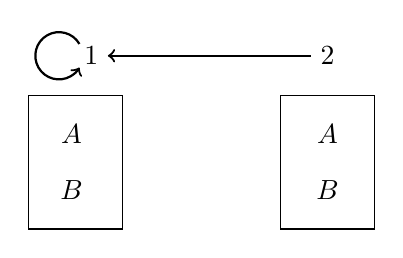
\begin{tikzpicture}
		\node (atom1) at (0,1) {1};
		\node (atom2) at (3,1) {2};
		\node (atom3) at (-0.25,0) {$A$};
		\node (atom4) at (3,0) {$\enot A$};
		\node (atom5) at (-0.25,-0.7) {$\enot B$};
		\node (atom6) at (3,-0.7) {$B$};
		\draw[->, thick] (atom1)+(-0.15,0.15) arc (-330:-30:.3);
		%\draw[->, thick] (atom2)+(0.15,-0.15) arc (-150:150:.3); 
		\draw[<-, thick] (atom1) -- (atom2);
		\draw (-0.8,-1.2) rectangle (0.4,0.5);
		\draw (2.4,-1.2) rectangle (3.6,0.5);
	\end{tikzpicture}
\end{center}
Qual a interpretação deste diagrama? Ele contém apenas dois mundos, 1 e 2. As setas entre os mundos indicam a relação de acessibilidade. Os mundos 1 e 2 acessam o mundo 1, mas nem 1 nem 2 acessam o mundo 2. As caixas em cada mundo nos permitem saber quais sentenças atômicas são verdadeiras em cada mundo: `$A$' é verdadeira em 1 mas  falsa em 2; `$B$' é falsa em 1 mas verdadeira em 2. Você só pode escrever uma sentença atômica ou a negação dela  em cada uma dessas caixas. A partir daí, podemos descobrir facilmente quais são os valores de verdade das sentenças complexas em cada mundo. Por exemplo, nessa interpretação, todas as sentenças a seguir são verdadeiras em $w_1$: 
 
\begin{itemize}
	\item[]$A\eand\enot B$, \,\,\, $B\eif A$, \,\,\, $\ediamond A$, \,\,\, $\ebox\enot B$
\end{itemize}
Se você não gosta de pensar através de diagramas, pode então expressar essa mesma interpretação assim:
\begin{itemize}
	\item[$W$:]$1,2$
	\item[$R$:]$\langle 1,1\rangle, \langle 2,1\rangle$
	\item[]$\nu_{1}(A)=V, \nu_{2}(B)=F, \nu_{2}(A)=F, \nu_{2}(B)=V$
\end{itemize}
Você terá a chance de preparar suas próprias interpretações 
em breve, quando começarmos a olhar para \emph{contrainterpretações}.


%%%\section{Uma semântica para o Sistema  K}

\section{Uma semântica para o sistema \mlK}
\label{SemanticsK}

Agora podemos estender todos os conceitos semânticos da  LVF para cobrir também a LM:
\factoidbox{
	\begin{itemize}
		\item  $\metav{A}_1,\metav{A}_2, \dots \metav{A}_n\therefore\metav{C}$ é \textit{valido em k} se e somente se não há nenhum mundo em nenhuma interpretação em que $\metav{A}_1,\metav{A}_2, \dots \metav{A}_n$ são todas verdadeiras e $\metav{C}$ é falsa.

		\item $\metav{A}$ é uma \textit{validade logica em k} se e somente se $\metav{A}$ é verdadeira em todos os  mundos e   em todas as interpretações.

		\item $\metav{A}$ é uma \textit{contradicao em k} se e somente se $\metav{A}$ é falsa em todos os mundos e em todas as interpretações.

		\item $\metav{A}_1,\metav{A}_2, \dots \metav{A}_n$ são \textit{compativeis em k} se e somente se há algum mundo em alguma interpretação em que todas são verdadeiras.
	\end{itemize}
}


 Também podemos estender o uso de `$\entails$'. Para isso, precisamos adicionar subscritos da mesma forma como fizemos com `$\proves$'. Assim, quando quisermos dizer que o argumento $\metav{A}_1,\metav{A}_2, \dots \metav{A}_n\therefore\metav{C}$  é válido em \mlK, escreveremos: $\metav{A}_1,\metav{A}_2, \dots \metav{A}_n\entails_\mlK\metav{C}$. 


Para se ter uma ideia melhor desses conceitos semânticos, vejamos algumas contrainterpretações. Considere a seguinte afirmação (falsa):

\begin{itemize}
	\item[]
	      \begin{itemize}
		      \item[]$\enot A\entails_\mlK \enot \ediamond A$
	      \end{itemize}
\end{itemize}
Como obter uma contrainterpretação para essa afirmação? Precisamos construir uma interpretação na qual `$\enot A$' é verdadeira em algum mundo $w$, e `$\enot\ediamond A$ é falsa   nesse mundo $w$. Aqui está uma dessas interpretações, apresentada em um diagrama:
\begin{center}
	\begin{tikzpicture}
		\node (atom1) at (0,1) {1};
		\node (atom2) at (3,1) {2};
		\node (atom3) at (-0.25,0) {$\enot A$};
		\node (atom4) at (3,0) {$A$};
		\draw[->, thick] (atom1) -- (atom2);
		\draw (-0.8,-0.6) rectangle (0.4,0.5);
		\draw (2.4,-0.6) rectangle (3.6,0.5);
	\end{tikzpicture}
\end{center}
É fácil ver que isso funciona como uma contrainterpretação para  $\enot A\entails_\mlK\enot\ediamond A$. Em primeiro lugar, `$\enot A$' é verdadeira no mundo $1$. 
E, em segundo lugar, como `$A$' é verdadeira em $2$ e $2$ é acessível a partir de $1$, então temos que `$\ediamond A$' é verdadeira em $1$, e consequentemente `$\enot\ediamond A$'   é falsa em $1$. 
Portanto, há algum mundo nessa interpretação onde `$\enot A$' é verdadeira e `$\enot\ediamond A$'  falsa, e, por isso,     
$\enot A\nentails_\mlK \enot \ediamond A$.


Por que escolhemos o subscrito \mlK? Existe uma relação importante entre o sistema \mlK{} e a definição de validade que acabamos de fornecer. Em particular, temos os dois resultados a seguir:
\begin{itemize}
	\item Se $\metav{A}_1,\metav{A}_2, \dots \metav{A}_n\proves_\mlK\metav{C}$, então $\metav{A}_1,\metav{A}_2, \dots \metav{A}_n\entails_\mlK\metav{C}$
	\item Se $\metav{A}_1,\metav{A}_2, \dots \metav{A}_n\entails_\mlK\metav{C}$, então $\metav{A}_1,\metav{A}_2, \dots \metav{A}_n\proves_\mlK\metav{C}$
\end{itemize}
O primeiro resultado é conhecido como \emph{correção}, pois nos diz que as regras de \mlK{} são boas e corretas: se você pode justificar um argumento fornecendo uma prova dele usando o sistema \mlK, então esse argumento é realmente válido. O segundo resultado é conhecido como    \emph{completude}, uma vez que nos diz que as regras de \mlK{} são amplas o suficiente para capturar todos os argumentos válidos: se um argumento é válido, então será possível oferecer uma prova em \mlK{} que o justifique.
 

Chamamos atenção para o fato de que uma coisa é enunciar esses resultados, outra bem diferente é prová-los. Provar os teoremas da correção e completude para os sistemas modais está fora de nossos objetivos aqui, que são meramente introdutórios. Mas podemos, pelo menos, usar essa definição semântica de validade em  \mlK{} para entender melhor o funcionamento das subprovas estritas e das regras R$\mlK$ e  \ebox I.

Em uma subprova estrita, não  é permitido fazer uso de qualquer informação que esteja fora dela, exceto o que importamos para a subprova estrita usando a regra  R$\mlK$. Se tivermos assumido ou provado $\ebox \metav{A}$, então por  R$\mlK$ podemos usar a sentença  $\metav{A}$ dentro de uma subprova estrita. E em \mlK, essa é a única maneira de importar uma sentença para dentro de uma subprova estrita.
 Portanto, tudo o que pode ser provado dentro de uma subprova estrita deve seguir a partir de uma  sentença  $\metav{A}$ onde fora da subprova estrita temos $\ebox \metav{A}$.
 Assim, seguindo o raciocínio acima, se provamos uma sentença $\metav{B}$ dentro da subprova estrita, $\metav{B}$ depende apenas da  uma sentença $\metav{A}$ onde fora da subprova estrita temos $\ebox\metav{A}$.  Nessas condições, podemos obter  $\ebox\metav{B}$,  por \ebox I.
 
  Vamos imaginar agora que estejamos raciocinando sobre o que é verdade em um mundo possível em alguma interpretação. Se sabemos que $\ebox\metav{A}$ é verdadeira em um mundo possível $w$, então sabemos que $\metav{A}$ e, consequenteme, $\metav{B}$  são verdadeiras em todos os mundos acessíveis a ele.
  Portanto, como tudo o que for provado dentro de uma subprova estrita é verdadeiro em todos os mundos possíveis acessíveis a $w$, então $\ebox\metav{B}$ é verdadeira $w$. É por isso que \ebox I é uma regra correta.

%%%%%\section{Uma semântica para o sistema T}

\section{Uma semântica para o sistema \mlT}
\label{SemanticsT}

Dissemos que o sistema \mlK{} é correto e completo em relação à definição de validade que demos acima. Mas,  o que podemos afirmar sobre os outros sistemas modais \mlT, \mlSfour{}  e \mlSfive  ? Bem, eles são todos  \emph{incorretos} com respeito a essa definição de validade. Por exemplo, todos esses sistemas permitem inferir $A$ a partir de $\ebox A$, embora  $\ebox A\nentails_\mlK A$.

Isso significa que esses sistemas são uma perda de tempo? De jeito nenhum! Significa apenas que cada um dos sistemas \mlK{}, \mlT, \mlSfour{}  e \mlSfive{} formaliza uma noção de validade diferente, $\entails_\mlK$, $\entails_\mlT$, $\entails_\mlSfour$ e $\entails_\mlSfive$, cada uma delas é correta e completa com relação ao seu respectivo sistema. Então, para lidar com os outros sistemas precisamos modificar nossa definição de `$\entails$', assim como, as definições de validade lógica, contradição e compatibilidade entre sentenças.  
É nesta tarefa que a  relação de acessibilidade mostrará sua utilidade.  

Quando introduzimos a ideia de uma relação de acessibilidade, dissemos que poderia ser qualquer relação entre mundos de que você goste:  em uma interpretação a relação de acessibilidade pode ligar todos os mundos, relacionando cada um com todos os outros; em outra interpretação ela pode separar todos os mundos, não relacionando nenhum mundo com nenhum outro. E ela pode situar-se em qualquer ponto entre esses dois extremos. É assim, com esta ampla flexibilidade, que as relações de acessibilidade funcionam em nossa definição de $\entails_\mlK$. 

Mas se quisermos, podemos colocar algumas restrições nas relações de acessibilidade que podem fazer parte das interpretações. Podemos, por exemplo, exigir que as relações de acessibilidade sejam sempre \emph{reflexivas}:

\begin{itemize}
	\item $\forall wRww$
\end{itemize}
Isto significa que todo mundo acessa ele próprio.  Com   essa restrição podemos introduzir uma nova relação de consequência, $\entails_\mlT$, como segue:
\factoidbox{
	$\metav{A}_1,\metav{A}_2, \dots \metav{A}_n\entails_\mlT \metav{C}$  se e somente se  não existe nenhum mundo em qualquer interpretação \emph{que tenha uma relação de acessibilidade reflexiva}, na qual $\metav{A}_1,\metav{A}_2, \dots \metav{A}_n$ são todas verdadeiras e $\metav{C}$ é falsa.
}
Anexamos o subscrito \mlT{}  a `$\entails$' porque verifica-se que o sistema \mlT{} é correto e completo em relação a esta nova definição de validade:
\begin{itemize}
	\item Se $\metav{A}_1,\metav{A}_2, \dots \metav{A}_n\proves_\mlT\metav{C}$, então $\metav{A}_1,\metav{A}_2, \dots \metav{A}_n\entails_\mlT\metav{C}$
	\item Se $\metav{A}_1,\metav{A}_2, \dots \metav{A}_n\entails_\mlT\metav{C}$, então $\metav{A}_1,\metav{A}_2, \dots \metav{A}_n\proves_\mlT\metav{C}$
\end{itemize}
Como antes, não provaremos os resultados de correção e completude. 

Lembramos que o sistema \mlT{} é uma extensão de \mlK{} (Seção \ref{T})  e na seção anterior apresentamos um esboço da correção da  regra \ebox I.  Agora, mostraremos  que a regra  \ebox E é correta, se a relação de acessibilidade for reflexiva.  

\factoidbox{
	\[\begin{nd}
			\have[m]{m}{\ebox \metav{A}}
			\have[\, ]{n}{\metav{A}}\boxe{m}
		\end{nd}\]
}
Para justificar a regra \ebox E, é suficiente mostrar que não existe uma  contrainterpretação para:
\[
	\ebox \metav{A}\entails_\mlT \metav{A}
\]
 
 Caso existisse,  precisaríamos construir  uma interpretação  na qual $\ebox \metav{A}$ fosse verdadeira em algum  mundo  $w$, mas $\metav{A}$ fosse falsa nesse mundo.  Neste caso teríamos:

  \begin{itemize}
	\item[(1)]  $\ebox \metav{A}$ é verdadeira em $w$   \,\,\,\,\,\,  e \,\,\,\,\,\,  (2)\, $\metav{A}$  é falsa em $w$.   
\end{itemize}
Mas, como como a relação de acessibilidade é reflexiva, $w$ acessa $w$, logo: 
\begin{itemize}
	\item[(3)]  $Rww$.
\end{itemize}
De (1) podemos concluir que $\metav{A}$ deve ser verdadeira em todos os mundos acessíveis a $w$, em particular nele próprio,  pois em (3) temos que $Rww$. Logo:
\begin{itemize}
	\item[(4)]   $\metav{A}$ é verdadeira em $w$.
\end{itemize}
De (2) e  (4) chegamos a uma contradição!  Portanto, não há uma interpretação  na qual $\ebox\metav{A}$ seja verdadeira em um dado mundo, mas  $\metav{A}$  falsa nesse mundo. Consequentemente,   $\ebox \metav{A}\entails_\mlT \metav{A}$ é válido.


%%%% \section{Uma semântica para S4}

\section{Uma semântica para o sistema \mlSfour}
\label{SemanticsS4}

De que outra forma podemos ajustar nossa definição de validade? Podemos também estipular que a relação de acessibilidade seja \emph{transitiva}:
\begin{itemize}
	\item $\forall w_1\forall w_2\forall w_3 ((Rw_1w_2 \eand Rw_2w_3)\eif Rw_1w_3)$
\end{itemize}
Isso significa que se  $w_1$ acessa $w_2$, e $w_2$ acessa $w_3$, então  $w_1$ acessa $w_3$. Ou seja, a acessibilidade entre mundos forma cadeias de acessibilidade indireta e todos os mundos nessas cadeias devem ser levados em consideração na decisão sobre se algo é possível ou não. Com essa restrição imposta  à nossa relação de acessibilidade, temos uma nova relação de consequência, $\entails_\mlSfour$, como segue:
\factoidbox{
	$\metav{A}_1,\metav{A}_2, \dots \metav{A}_n\entails_\mlSfour \metav{C}$ se e somente se não existe nenhum mundo em qualquer interpretação \emph{que tenha uma relação de acessibilidade reflexiva e transitiva}, na qual $\metav{A}_1,\metav{A}_2, \dots \metav{A}_n$ são todas verdadeiras e $\metav{C}$ é falsa
}
Anexamos o subscrito \mlSfour{}  a `$\entails$' porque verifica-se que o sistema \mlSfour{} é correto e completo em relação a esta nova definição de validade:
\begin{itemize}
	\item Se $\metav{A}_1,\metav{A}_2, \dots \metav{A}_n\proves_\mlSfour\metav{C}$, então $\metav{A}_1,\metav{A}_2, \dots \metav{A}_n\entails_\mlSfour\metav{C}$
	\item Se $\metav{A}_1,\metav{A}_2, \dots \metav{A}_n\entails_\mlSfour\metav{C}$, então $\metav{A}_1,\metav{A}_2, \dots \metav{A}_n\proves_\mlSfour\metav{C}$
\end{itemize}
Como antes, não provaremos esses resultados. Daremos apenas uma ideia de como mostrar que as regras de inferência de \mlSfour{} são corretas.

Ora, vimos na Seção \ref{S4} que o sistema \mlSfour{} é uma extensão de \mlT{} e já mostramos na seção anterior que  a regra  \ebox E é correta quando a relação de acessibilidade é reflexiva; e é relativamente fácil justificar  a regra  R$\mathbf{4}$, se a relação de acessibilidade for transitiva.

 
\factoidbox{
	\[\begin{nd}
			\have[m]{m}{\ebox\metav{A}}
			\open
			\hypo[\ ]{k}{\ebox}
			\have[\ ]{n}{\ebox\metav{A}}\rfour{m}
		\end{nd}\]
}

Lembramos que a ideia por trás das subprovas estritas é que elas são maneiras de provar coisas que devem ser verdadeiras em todos os mundos acessíveis. Assim, a regra R$\mathbf{4}$  significa que sempre que $\ebox \metav{A}$ for verdadeira em um mundo, $\ebox \metav{A}$ também deve ser verdadeira  em todos os mundos acessíveis  a este mundo. Logo, devemos ter $\ebox\metav{A} \entails_\mlSfour \ebox\ebox\metav{A}$.

Para constatar isso, tente construir uma contrainterpretação para esta afirmação:
\begin{itemize}
	\item[]$\ebox\metav{A} \entails_\mlSfour \ebox \ebox \metav{A}$
\end{itemize}
 

 Precisaríamos construir uma interpretação na qual $\ebox\metav{A}$ seja verdadeira em um dado mundo  $w_1$, mas  $\ebox \ebox \metav{A}$  falsa nesse mundo. Assim teríamos: 
 \begin{itemize}
	\item[(1)]  $\ebox\metav{A}$ é verdadeira em $w_1$ \,\,\,\,\,\,  e \,\,\,\,\,\,  (2)\, $\ebox \ebox \metav{A}$  é  falsa em  $w_1$.
\end{itemize} 
De (2) se segue que $w_1$ deve acessar algum mundo $w_2$, no qual $\ebox\metav{A}$ é falsa.  Logo, existe um $w_2$ tal que: 
\begin{itemize}
	\item[(3)]  $Rw_1w_2$  \,\,\,\,\,\,  e \,\,\,\,\,\,  (4)\, $\ebox\metav{A}$ é falsa em $w_2$.
\end{itemize}
De (4) podemos concluir que $w_2$ deve acessar algum mundo  $w_3$, no qual $\metav{A}$ é falsa. 
Logo, existe um $w_3$ tal que:
\begin{itemize}
	\item[(5)]  $Rw_2w_3$  \,\,\,\,\,\, e  \,\,\,\,\,\, (6)\,  $\metav{A}$ é falsa em $w_3$.
\end{itemize}
Como a relação de acessibilidade é transitiva, de (3) e (5) temo que $w_1$ acessa $w_3$, isto é: 
\begin{itemize}
	\item[(7)]  $Rw_1w_3$.
\end{itemize}
Mas,  de (1) podemos concluir que  $\metav{A}$  é verdadeira em todo mudo acessível a $w_1$, em particular, verdadeira em $w_3$. Assim: 
\begin{itemize}
	\item[(8)]  $\metav{A}$  é verdadeira em $w_3$.
\end{itemize}
 De (6) e (8), temos que  $\metav{A}$ é verdadeira e falsa em $w_3$. Contradição!  
  

Portanto, não há uma interpretação  na qual $\ebox\metav{A}$ seja verdadeira em um dado mundo, mas  $\ebox \ebox \metav{A}$  falsa nesse mundo. Consequentemente,  $\ebox\metav{A} \entails_\mlSfour \ebox\ebox\metav{A}$ é válido.


%%%% \section{Uma semântica para S5}
\section{Uma semântica para o sistema \mlSfive}
\label{SemanticsS5}

Vamos acrescentar mais uma restrição à relação de acessibilidade. Desta vez, impor que a relação de acessibilidade seja também \emph{simétrica}:
\begin{itemize}
	\item $\forall w_1\forall w_2(Rw_1w_2 \eif Rw_2w_1)$
\end{itemize}
Isto significa que se  $w_1$ acessa $w_2$, então $w_2$ acessa  $w_1$. Os lógicos chamam uma relação que é reflexiva, simétrica e transitiva de \emph{relação de equivalência}. Agora podemos  definir uma nova relação de consequência, $\entails_\mlSfive $, como segue:

\factoidbox{
	$\metav{A}_1,\metav{A}_2, \dots \metav{A}_n\entails_\mlSfive  \metav{C}$ se e somente se  não existe nenhum mundo em qualquer interpretação \emph{cuja relação de acessibilidade seja uma relação de equivalência}, na qual $\metav{A}_1,\metav{A}_2, \dots \metav{A}_n$ são todas verdadeiras e $\metav{C}$ é falsa.
}
Anexamos o subscrito \mlSfive{} a `$\entails$' porque  o sistema \mlSfive{} é correto e completo em relação a esta nova definição de validade:

\begin{itemize}
	\item Se $\metav{A}_1,\metav{A}_2, \dots \metav{A}_n\proves_\mlSfive \metav{C}$, então $\metav{A}_1,\metav{A}_2, \dots \metav{A}_n\entails_\mlSfive \metav{C}$
	\item Se $\metav{A}_1,\metav{A}_2, \dots \metav{A}_n\entails_\mlSfive \metav{C}$, então $\metav{A}_1,\metav{A}_2, \dots \metav{A}_n\proves_\mlSfive \metav{C}$
\end{itemize}
Aqui também não provaremos esses resultados.  No entanto, é relativamente fácil  justificar  a  regra   R$\mathbf{5}$,  se a relação de acessibilidade for uma relação de equivalência.

\factoidbox{
	\[\begin{nd}
			\have[m]{m}{\enot\ebox \metav{A}}
			\open
			\hypo[\ ]{k}{\ebox}
			\have[\, ]{n}{\enot\ebox\metav{A}}\rfive{m}
		\end{nd}\]
}


Essa regra diz que se $\metav{A}$ não é necessária, ou seja, falsa em algum mundo acessível, também não é necessária em qualquer mundo possível acessível. 
 Temos então $\enot\ebox \metav{A} \entails_\mlSfive \ebox\enot\ebox \metav{A}$.

Para constatar isso, tente construir uma contrainterpretação para esta afirmação:
\[
	\enot\ebox\metav{A} \entails_\mlSfive  \ebox \enot\ebox \metav{A}
\]
 
 

Precisaríamos construir uma interpretação  na qual  $\enot\ebox\metav{A}$ é verdadeira em um mundo $w_1$, mas  $\ebox \enot\ebox \metav{A}$  é falsa nesse mundo. Assim teríamos:

  \begin{itemize}
	\item[(1)]  $\enot\ebox\metav{A}$ é verdadeira em $w_1$   \,\,\,\,\,\,  e \,\,\,\,\,\,  (2)\, $\ebox \enot\ebox \metav{A}$  é falsa em $w_1$.   
\end{itemize} 
De (1) se segue que $\ebox\metav{A}$ é falsa em  $w_1$. Assim, $w_1$  deve acessar algum mundo $w_2$, no qual $\metav{A}$ é falsa. Logo existe um mundo $w_2$ tal que:
 \begin{itemize}
	\item[(3)]  $Rw_1w_2$      \,\,\,\,\,\,  e \,\,\,\,\,\,  (4)\, $\metav{A}$ é falsa em $w_2$.  
\end{itemize} 
De (2), podemos concluir que $w_1$ deve acessar algum mundo $w_3$, no qual $\enot\ebox \metav{A}$ é falsa. Logo,  existe um mundo $w_3$ tal que:
 \begin{itemize}
	\item[(5)]  $Rw_1w_3$   \,\,\,\,\,\,  e \,\,\,\,\,\,  (6)\, $\enot\ebox \metav{A}$ é falsa em $w_3$.  
\end{itemize} 
Como agora temos a restrição que a relação de acessibilidade é uma relação de equivalência e, portanto, simétrica,  de (5) podemos inferir que $w_3$ acessa  $w_1$. Ou seja:
\begin{itemize}
	\item[(7)]   $Rw_3w_1$. 
\end{itemize}
Como  $R$ é uma relação de equivalência,  $R$ é transitiva. Assim de (7) e (3) podemos inferir  que $w_3$ acessa $w_2$. Assim,   temos:
 \begin{itemize}
	\item[(8)]   $Rw_3w_2$     
\end{itemize} 
 Mas, de (6) se segue que $\ebox \metav{A}$   é verdadeira em $w_3$ e consequentemente, $\metav{A}$ é verdadeira em todos os mundos que $w_3$ acessa, em particular $w_2$, pois em (8) temos que $Rw_3w_2$. Logo:
 \begin{itemize}
	\item[(9)]  $\metav{A}$ é verdadeira em $w_2$.        
\end{itemize} 
De (4)  e (9) chegamos à uma Contradição!
Portanto, não há uma interpretação  na qual $\enot\ebox\metav{A}$ seja verdadeira em um dado mundo, mas  $\ebox \enot\ebox \metav{A}$  falsa nesse mundo. Consequentemente,  $\enot\ebox \metav{A} \entails_\mlSfive \ebox\enot\ebox \metav{A}$ é válido. \\

Na definição de  $\entails_\mlSfive $, estipulamos que a relação de acessibilidade deve ser uma relação de equivalência. Mas acontece que há outra maneira de obter uma noção de validade adequada para \mlSfive. Em vez de estipular que a relação de acessibilidade seja uma relação de equivalência, podemos estipular que seja uma relação \emph{universal}:
\begin{itemize}
	\item $\forall w_1\forall w_2Rw_1w_2$
\end{itemize}
Isto significa  que todo mundo acessa todo mundo. Usando essa restrição na relação de acessibilidade, poderíamos ter definido  $\entails_\mlSfive $ assim:\factoidbox{
	$\metav{A}_1,\metav{A}_2, \dots \metav{A}_n\entails_\mlSfive  \metav{C}$ se e somente se  não existe nenhum mundo em qualquer interpretação  \emph{que tenha uma relação de acessibilidade universal}, na qual $\metav{A}_1,\metav{A}_2, \dots \metav{A}_n$ são todas verdadeiras e $\metav{C}$ é falsa.
}
Se definíssemos $\entails_\mlSfive $ assim, ainda obteríamos os mesmos resultados de correção e completude para \mlSfive{}. O que isso nos diz? Isso significa que o sistema \mlSfive{} é aquele que formaliza as noções de necessidade e possibilidade absolutas, nas quais ser possível é ocorrer em algum mundo qualquer e ser necessário é ocorrer em todos os mundos. Todos os outros sistemas (\mlK{}, \mlT{} e \mlSfour) representam algum grau de relativização destas noções de necessidade e possibilidade.
 Além disso, a maioria dos filósofos assume que as noções de necessidade com as quais estão mais preocupados, como a  \emph{necessidade lógica} e a \emph{necessidade metafísica}, são exatamente desse tipo. Portanto, \mlSfive{} é o sistema modal que a maioria dos filósofos usa na maior parte do tempo.
 

\practiceproblems

\problempart
Apresente contrainterpretações para as quatro seguintes afirmações falsas:
\begin{earg}
	\item $\enot P \entails_\mlK \enot\ediamond P$
	\item $\ebox(P \eor Q)\entails_\mlK \ebox P \eor \ebox Q$
	\item $\entails_\mlK \enot \ebox (A\eand \enot A)$
	\item $\ebox A\entails_\mlK A$
\end{earg}

\problempart
Apresente contrainterpretações para as duas seguintes afirmações falsas:
\begin{earg}
	\item $\ebox (M\eif O),\ediamond M\entails_\mlT O$
	\item $\ebox A\entails_\mlT \ebox \ebox A$
\end{earg}

\problempart
Apresente contrainterpretações para as duas seguintes afirmações falsas:
\begin{earg}
	\item $\ediamond A\entails_\mlSfour \ebox\ediamond A$
	\item $\ediamond A, \ebox (\ediamond A \eif B)\entails_\mlSfour\ebox B$
\end{earg}

\section*{Leitura adicional}

A lógica modal é um grande subcampo da lógica. Nós apenas arranhamos a superfície. Se você quiser aprender mais sobre lógica modal, aqui estão alguns livros que você pode consultar:

\begin{itemize}
	\item Hughes, G. E., \& Cresswell, M. J. (1996). \emph{A New Introduction to Modal Logic}, Oxford: Routledge.
	\item Priest, G. (2008). \emph{An Introduction to Non-Classical Logic}, 2nd ed., Cambridge: Cambridge University Press.
	\item Garson, J. W. (2013). \emph{Modal Logic for Philosophers}, 2nd ed., Cambridge: Cambridge University Press.
\end{itemize}

Nenhum desses autores formula seus sistemas de provas modais da mesma forma que nós, mas a formulação mais próxima é dada por Garson. 







%!TEX root = forallxyyc.tex
\part{Metateoria}
\label{ch.normalform}
\addtocontents{toc}{\protect\mbox{}\protect\hrulefill\par}

\chapter{Formas normais}


\section{Forma Normal Disjuntiva}\label{s:DNFDefined}

Às vezes é útil considerar grupos restritos de sentenças com formas particularmente simples.
Por exemplo, podemos considerar o grupo restrito formado pelas sentenças atômicas e pelas sentenças que são negações de sentenças atômicas:
$$A, \enot B, A_3, \enot F_2, ...$$
As sentenças deste grupo  são comumente chamadas de \xdefine{literais}.
Podemos criar um grupo mais amplo, acrescentando aos literais sentenças que são conjunções arbitrárias de literais:
	\begin{align*}
			& A_3 \\
			& A \eand \enot B \\
			& \enot C \\
			& \enot J \eand \enot A_3 \eand  C \\
			& F_2 \eand  J \\
			& \ \ \vdots
	\end{align*}
Podemos ampliar mais um pouco este grupo e acrescentar a ele sentenças que são disjunções de literais ou de conjunções arbitrárias de literais:
	\begin{align*}
  		& A \\
  		& A \eand \lnot B \eand C\\
  		& (A \eand B) \eor (A \eand \enot B)\\
  		& (A \eand B) \eor (A \eand  B \eand C \eand \enot D \eand \enot E)\\
  		& A \eor (C \eand \enot P_{234} \eand P_{233} \eand Q) \eor \enot B\\
  		& \ \ \vdots
	\end{align*}
Dizemos que as sentenças deste grupo mais amplo estão na \define{disjunctive normal form}, cuja definição formal pode ser assim apresentada:
uma sentença está na \textit{forma normal disjuntiva} se e somente se ela satisfizer todas as seguintes condições:
	\begin{earg}
		\item[(\textsc{fnd 1})] Nenhum conectivo que não seja negação, conjunção ou disjunção ocorre na sentença;
		\item[(\textsc{fnd 2})] Qualquer negação que ocorra na sentença é a negação de uma letra sentencial;
		\item[(\textsc{fnd 3})] Qualquer conjunção que ocorra na sentença é conjunção de literais; ou seja, apenas sentenças atômicas ou negações de sentenças atômicas podem ser conjuntos das conjunções.
	\end{earg}
Um outro modo de entender o grupo de sentenças que estão na forma normal disjuntiva é definindo-o como o grupo composto pelas sentenças que pertencem a qualquer um dos seguintes 4 grupos:
\begin{earg}
		\item[\textsc{grupo 1} - letras sentenciais:] \ \\
				$B_3, A, J_7, C, P_5,...$
		\item[\textsc{grupo 2} - negações de sentenças do grupo anterior:] \ \\
				$\enot A, \enot B_9, \enot K_2, \enot J,... $
		\item[\textsc{grupo 3} - conjunção de sentenças dos grupos anteriores:] \ \\
				$(B_3 \eand C), \ (\enot S \eand A \eand \enot C_1),...$
		\item[\textsc{grupo 4} - disjunção de sentenças dos grupos anteriores:] \ \\ 
				$(A \eand B) \eor (A \eand \enot B),\ \  A \eor (C \eand \enot P_{234} \eand P_{233} \eand Q) \eor \enot B,...$
	\end{earg}
Repare que estamos \emph{temporariamente} desrespeitando a gramática da LVF aqui. 
Nos exemplos acima, empregamos conjunções e disjunções com mais de dois itens sem os necessários parênteses intermediários.
Estritamente falando, `$(A \eand B \eand C)$', por exemplo, não é uma sentença gramaticalmente correta. Ela teria que ter sido escrita ou como `$((A \eand B) \eand C)$' ou como `$(A \eand (B \eand C))$'. 
E o mesmo ocorre com as disjunções com mais de dois disjuntos.
Vamos continuar desconsiderando os parênteses intermediários em disjunções e conjunções com mais de duas partes porque isso facilita o reconhecimento das sentenças na forma normal disjuntiva e, além disso, todos os diferentes modos possíveis de preencher os parênteses nestes casos levam a sentenças logicamente equivalentes.

A seguinte notação nos ajudará a termos uma intuição visual de como são as sentenças na forma normal disjuntiva.
Escrevemos `$\pm \meta{A}$' para indicar que $\meta{A}$ é um literal, ou seja, $\meta{A}$ é uma letra sentencial ou a negação de uma letra sentencial.
Então, uma sentença na forma normal disjuntiva tem o seguinte aspecto geral:
	$$(\pm \meta{A}_1 \land \ldots \land \pm \meta{A}_i) \lor (\pm \meta{A}_{i+1} \land \ldots \land \pm\meta{A}_j) \lor \ldots \lor (\pm\meta{A}_{m+1} \land \ldots \land \pm \meta{A}_n)$$
Veja que o aspecto mais geral de uma sentença na forma normal disjuntiva é o de uma disjunção de conjunções de literais.
Mas esta é só uma intuição visual, já que qualquer sentença pertencente a  qualquer um dos quatro grupos descritos acima está na forma normal disjuntiva.

As sentenças na forma normal disjuntiva satisfazem a seguinte propriedade:
	\factoidbox{\label{thm:dnf}\textbf{Teorema da Formal Normal Disjuntiva.} Dada qualquer sentença da LVF, existe uma sentença logicamente equivalente a ela que está na forma normal disjuntiva.
	}
Daqui para a frente iremos abreviar a expressão  `forma normal disjuntiva' por `FND'. 


\section{Prova do Teorema FND}
\label{s:DNFTruthTable}

Usaremos as tabelas de verdade para construirmos uma prova do Teorema da FND.
A ideia é que dada uma sentença qualquer, podemos utilizar sua tabela de verdade como fonte para produzir uma sentença na FND com tabela de verdade idêntica e que, por isso, será logicamente equivalente à sentença original.
Vamos inicialmente ilustrar como isto é feito e, em seguida, transformar essa ilustração em uma prova rigorosa.

Considere uma sentença $\meta{S}$ e suponha que $\meta{S}$ contém três letras sentencias:  `$A$', `$B$' e `$C$'.
O nosso primeiro passo é construir uma tabela de verdade completa para $\meta{S}$.
Suponha que $\meta{S}$ seja tal que sua tabela de verdade resulte em:
\begin{center}
\begin{tabular}{c c c | c}
$A$ & $B$ & $C$ & $\meta{S}$\\
\hline
 V & V & V & V \\
 V & V & F & F \\
 V & F & V & V \\
 V & F & F & F \\
 F & V & V & F \\
 F & V & F & F \\
 F & F & V & V \\
 F & F & F & V
\end{tabular}
\end{center}
%Now, consider a sentence, whose only connectives are negations and conjunctions, where no connective occurs within the scope of any negation, e.g.:
%	$$A \eand \enot B \eand C$$
%This sentence is true when, and only when, `$A$' is true, `$B$' is false and `$C$' is true. Similarly, the sentence:
%	$$\enot A \eand \enot B \eand C$$
%this is true when, and only when, `$A$' is false, `$B$' is false and `$C$' is true. 
%
%A disjunction is true when, and only when, at least one of the disjuncts is true. So if we write down a disjunction of sentences of the above form, perhaps
%	$$(A \eand \enot B \eand C) \eor (\enot A \eand \enot B \eand C)$$
%then it will be true on exactly \emph{two} lines of the truth table which describes all possible valuations of `$A$', `$B$' and `$C$'. 
%

\noindent Note que $\meta{S}$ é verdadeira em quatro linhas da tabela de verdade: nas linhas 1, 3, 7 e 8.
Na linha 1 de nossa tabela, as três letras sentencias `$A$', `$B$' e `$C$' são verdadeiras.
Utilizamos esta informação para construir uma sentença que será verdadeira nesta linha e falsa em todas as outras.
A sentença é: 
		$$A \eand B \eand C$$
Note que uma conjunção só é verdadeira quando todos os seus conjuntos são verdadeiros.
Então esta conjunção só será verdadeira quando `$A$', `$B$' e `$C$' forem.
Ou seja, só na linha 1 da tabela de $\meta{S}$.

Fazemos a mesma coisa com as outras linhas da tabela em que $\meta{S}$ é verdadeira.
A próxima delas  é a linha 3, onde as colunas de referência indicam que `$A$' é verdadeira, `$B$' é falsa e `$C$' é verdadeira.
Utilizamos esta informação para construir uma sentença que será verdadeira nesta linha e falsa em todas as outras.
A sentença é: 
		$$A \eand \enot B \eand C$$
Novamente, repare que uma conjunção só é verdadeira quando todos os seus conjuntos são verdadeiros. Então esta conjunção só será verdadeira quando `$A$' é verdadeira, `$B$' é falsa e `$C$' é verdadeira.
Ou seja, só na linha 3 da tabela de $\meta{S}$.

Fazendo a mesma coisa com as outras linhas da tabela nas quais $\meta{S}$ é verdadeira, as linhas 7 e 8, obtemos, respectivamente, as seguintes sentenças:
\begin{center}
		$\enot A \eand \enot B \eand C$ \\
		$\enot A \eand \enot B \eand \enot C$
\end{center}
%$$\enot A \eand \enot B \eand C$$
%$$\enot A \eand \enot B \eand \enot C$$
Então, o que fizemos até aqui foi que, dada a tabela de verdade de $\meta{S}$, para cada uma das linhas em que $\meta{S}$ é verdeira, construímos uma sentença que é verdadeira nesta linha e falsa em todas as outras:
	\begin{earg}
		\item[]   $A \eand B \eand C$ \hfill  -- \ \ \ \ \ \ verdadeira apenas na linha 1
		\item[]  $A \eand \enot B \eand C$ \hfill  -- \ \ \ \ \ \  verdadeira apenas na linha 3
		\item[]  $\enot A \eand \enot B \eand C$ \hfill  -- \ \ \ \ \ \  verdadeira apenas na linha 7
		\item[]  $\enot A \eand \enot B \eand \enot C$ \hfill  -- \ \ \ \ \ \  verdadeira apenas na linha 8
	\end{earg}
Fazendo uma disjunção destas 4 sentenças obtemos:
$$(A \eand B \eand C) \eor (A \eand \enot B \eand C) \eor (\enot A \eand \enot B \eand C) \eor (\enot A \eand \enot B \eand \enot C)$$
Repare que, devido à sua construção, esta sentença terá uma tabela de verdade idêntica à da sentença $\meta{S}$. Será verdadeira exatamente nas linhas 1, 3, 7 e 8, e falsa nas demais; exatamente como  $\meta{S}$.
Ou seja, esta sentença é logicamente equivalente a $\meta{S}$.
Repare também que esta sentença é uma disjunção de conjunções de literais. Ou seja, é uma sentença na FND.
Ela é, então, a sentença que queríamos.
Uma sentença na FND que é logicamente equivalente a $\meta{S}$.

Partimos de uma sentença qualquer e construímos uma sentença na FND logicamente equivalente à sentença original.
A estratégia que utilizamos para esta construção não depende de nenhuma característica específica de $\meta{S}$.
$\meta{S}$ é uma sentença qualquer e por isso nossa estratégia é completamente geral.
Podemos, então, utilizá-la como base para construir uma prova do teorema da forma normal disjuntiva da seguinte forma.

\subsection{Explicitando a prova do teorema da FND}
Considere  $\meta{S}$ uma sentença qualquer e $\meta{A}_1, \ldots, \meta{A}_n$ as letras sentenciais que ocorrem em $\meta{S}$.
Considere, também, a tabela de verdade de $\meta{S}$.
Para obter uma sentença na FND que seja logicamente equivalente a $\meta{S}$, há dois casos a tratar:
	\begin{enumerate}
		\item \emph{$\meta{S}$ é falsa em todas as linhas de sua tabela de verdade.} Neste caso  $\meta{S}$ é uma contradição.
		A sentença $(\meta{A}_1 \eand \enot \meta{A}_1)$ satisfaz as condições que buscamos.
		Está na FND e é logicamente equivalente a $\meta{S}$, já que também é uma contradição.
	
		\item\emph{$\meta{S}$ é verdadeira em pelo menos uma linha de sua tabela de verdade.}
		Neste caso, para cada linha $i$ da tabela de verdade de $\meta{S}$, seja $\meta{B}_i$ uma conjunção da forma
		$$(\pm\meta{A}_{1} \land \ldots \land \pm\meta{A}_{n})$$
		onde cada literal $\pm\meta{A}_{j}$ será da forma $\meta{A}_{j}$ ou $\enot\meta{A}_{j}$ conforme as seguinte regras:
			\begin{align*}
				\pm\meta{A}_{j}\text{ \ é \ }\meta{A}_{j}&\emph{ \ \ sse \ \ \ }\meta{A}_{j}\text{ é verdadeira na linha }i\\
				\pm\meta{A}_{j}\text{ \ é \ }\enot\meta{A}_{j}&\emph{ \ \ sse \ \ \ }\meta{A}_{j}\text{ é falsa na linha }i
			\end{align*}
		O objetivo destas regras é garantir que  $\meta{B_i}$ será verdadeira na (e somente na) linha $i$ da tabela de verdade de $\meta{S}$.
		
		Considere agora  $i_1$, $i_2$, \dots, $i_m$ os números das linhas da tabela de verdade onde $\meta{S}$ é \emph{verdadeira} e seja $\meta{D}$ a seguinte sentença:
		$$\meta{B}_{i_1} \eor \meta{B}_{i_2} \eor \ldots \eor \meta{B}_{i_m}$$
		Como estamos considerando o caso 2, em que $\meta{S}$ é verdadeira em pelo menos uma linha de sua tabela de verdade, a sentença $\meta{D}$ está, por isso, bem definida.
		$\meta{D}$ é, em geral, uma disjunção de conjunções de literais e no caso limite, quando $\meta{S}$ é verdadeira em apenas uma linha de sua tabela, $\meta{D}$ é uma conjunção de literais.
		Seja qual for o caso, $\meta{D}$ está na FND.
		
		Além disso, a construção de $\meta{D}$ assegura também que, para cada linha~$i$ da tabela de verdade, $\meta{S}$ é verdadeira na linha $i$ \emph{se e somente se} um dos disjuntos de $\meta{D}$ (a saber, $\meta{B_i}$) é verdadeiro na, e somente na, linha $i$.
		Portanto, $\meta{S}$ e $\meta{D}$ têm a mesma tabela de verdade e são, por isso, logicamente equivalentes.
	\end{enumerate}
	Esses dois casos esgotam todas as possibilidades para a tabela de $\meta{S}$ e em ambos obtivemos uma sentença na FND que é logicamente equivalente a $\meta{S}$.
	Eles garantem, portanto, que dada qualquer sentença $\meta{S}$ há uma sentença na FND que é equivalente a $\meta{S}$. E isso finaliza a nossa prova do teorema da forma normal disjuntiva.

%So we have proved the DNF Theorem. Before we say any more, though, we should immediately flag that we are hereby returning to the austere definition of a (TFL) sentence, according to which we can assume that any conjunction has exactly two conjuncts, and any disjunction has exactly two disjuncts.



\section{Forma Normal Conjuntiva}
\label{s:CNF}

Existem outras formas normais além da \emph{disjuntiva}.
Uma que merece nossa atenção é a \emph{forma normal conjuntiva} (FNC).
A definição de FNC é muito parecida à definição da FND.
Uma sentença está na FNC se e somente se ela satisfaz todas as seguintes condições:
	\begin{earg}
		\item[(\textsc{fnc 1})] Nenhum conectivo que não seja negação, conjunção ou disjunção ocorre na sentença;
		\item[(\textsc{fnc 2})] Qualquer negação que ocorra na sentença é negação de uma letra sentencial;
		\item[(\textsc{fnc 3})] Qualquer disjunção que ocorra na sentença tem literais como disjuntos; ou seja, apenas sentenças atômicas ou negações de sentenças atômicas podem ser disjuntos das disjunções.
	\end{earg}

\noindent A definição da FNC é, portanto, absolutamente análoga à definição da FND, com a única diferença de que as conjunções e as disjunções trocaram de papel.
Ou seja, enquanto a forma geral das sentenças na FND é a de uma \textit{disjunção de conjunções} de literais, o aspecto mais geral de uma sentença na FNC será o de uma \textit{conjunção de disjunções} de literais:
$$(\pm \meta{A}_1 \lor \ldots \lor \pm \meta{A}_i) \land (\pm \meta{A}_{i+1} \lor \ldots \lor \pm\meta{A}_j) \land \ldots \land (\pm\meta{A}_{m+1} \lor\ldots \lor \pm \meta{A}_n)$$
lembrando que a notação $\pm\meta{A}_k$ indica que $\meta{A}_k$ é um literal, ou seja, uma letra sentencial ou a negação de uma letra sentencial.

Podemos agora propor e provar outro teorema sobre forma normal:
	\factoidbox{\label{thm:cnf}\textbf{Teorma da Forma Normal Conjuntiva.} Dada qualquer sentença da LVF, existe uma sentença logicamente equivalente a ela que está na forma normal conjuntiva.}

Seja $\meta{S}$ uma sentença LVF.
	\begin{itemize}
       	\item Começamos escrevendo a tabela de verdade completa para $\meta{S}$.
       	\item Se $\meta{S}$ é \emph{verdadeira} em todas as linhas da tabela de verdade, então $(\meta{A}_1 \eor \enot \meta{A}_1)$ satisfaz o teorema, já que está na FNC e é logicamente equivalente a $\meta{S}$.
       	\item Se $\meta{S}$ é \emph{falsa} em pelo menos uma linha da sua tabela de verdade, então, para cada linha onde $\meta{S}$ é falsa, escreva uma disjunção $(\pm\meta{A}_1 \eor \ldots \eor \pm\meta{A}_n)$ que seja \emph{falsa} nesta linha (e verdadeira em todas as outras).\footnote{
       	Quais devem ser as regras para a construção desta sentença? Tente descobrir. O que queremos aqui é o inverso do que fizemos na prova do teorema da FND.
       	Lá queríamos uma sentença verdadeira na linha especificada e falsa em todas as outras, que fosse uma conjunção de literais.
       	Aqui queremos uma sentença que é uma disjunção de literais, e que seja falsa na linha especificada e verdadeira em todas as outras.}
       	\item Considere $\meta{C}$ a conjunção de todas essas disjunções.
       	A construção de $\meta{C}$ garante que ela está na FNC e que sua tabela de verdade é idêntica à de $\meta{S}$, e que, por isso, $\meta{C}$ e $\meta{S}$ são logicamente equivalentes.
	\end{itemize}
       
 
\practiceproblems
\problempart
\label{pr.DNF}
Para cada uma das 6 sentenças abaixo apresente duas outras sentenças logicamente equivalentes à sentença original.
Uma delas na FND e outra na FNC.
	\begin{earg}
		\item $(A \eif \enot B)$
		\item $\enot (A \eiff B)$
		\item $(\enot A \eor \enot (A \eand B))$
		\item $(\enot (A \eif B ) \eand (A \eif C))$
		\item $(\enot (A \eor B) \eiff ((\enot C \eand \enot A) \eif \enot B))$
		\item $((\enot (A \eand \enot B) \eif C) \eand \enot (A \eand D))$
	\end{earg}

\chapter{Conectivos funcionalmente completos}
        
%\section{Adequação Expressiva da LVF}  

Dos conectivos da LVF, a engação, `$\enot$', é um conectivo de um lugar (unário), ou seja, liga-se a uma única sentença, e todos os outros são conectivos de dois lugares (binários) que se ligam a exatamente duas sentenças.
Mas nós podemos cogitar sobre conectivos de \textit{n} lugares (\textit{n}-ários), que ligam-se a $n$ sentenças.
Por exemplo, poderíamos propor um conectivo de três lugares, cujo símbolo poderia ser um coração, `$\heartsuit$', e estipular que ele tem a seguinte tabela de verdade característica:
\begin{center}
\begin{tabular}{c c c | c}
$A$ & $B$ & $C$ & $\heartsuit(A,B,C)$\\
\hline
 V & V & V & F \\
 V & V & F & V \\
 V & F & V & V \\
 V & F & F & F \\
 F & V & V & F \\
 F & V & F & V \\
 F & F & V & F \\
 F & F & F & F
\end{tabular}
\end{center}
Um tal conectivo, provavelmente, não corresponde nem aproximadamente a nenhuma expressão do português. Pelo menos não do jeito que `$\eand$' corresponde a `e', por exemplo.
Mas independentemente disso, há uma questão interessante a ser feita aqui. Suponha que nós queremos construir uma sentença que diz exatamente o que `$\heartsuit(A,B,C)$' diz.
Ou seja, suponha que queremos construir uma sentença tautologicamente equivalente a `$\heartsuit(A,B,C)$', cuja tabela é idêntica à tabela de `$\heartsuit(A,B,C)$'.
Será que para fazer isso nós precisamos adicionar à LVF o conectivo  `$\heartsuit$' e sua tabela característica?
Ou será que para dizer o que `$\heartsuit(A,B,C)$' diz, os conectivos que \emph{já existem} na LVF bastam?

Vamos refazer esta pergunta de um modo mais geral e preciso.
Antes disso, aqui vai um pouco de vocabulário.
Chamaremos um grupo de conectivos de \define{conjunto funcionalmente completo} se e somente se as sentenças construídas apenas com conectivos desse grupo são capazes de nos dar todas as tabelas de verdade possíveis.
Dito de outro modo, um conjunto de conectivos é \emph{funcionalmente completo} se e somente se dada qualquer tabela de verdade, existe alguma sentença com todos os seus conectivos pertencentes a este grupo e que tem exatamente esta tabela de verdade.

O ponto geral aqui é que quando um conjunto de conectivos é funcionalmente completo, podemos, com ele, construir sentenças que nos dão qualquer tabela de verdade.
Todas as tabelas de verdade são alcançáveis através de um conjunto de conectivos funcionalmente completo.
Então, o modo mais geral e preciso da pergunta feita acima é: será que o conjunto total de conectivos da LVF, $\{\enot, \eand, \eor, \eif, \eiff\}$, é funcionalmente completo?
	\factoidbox{\label{thm:ExpressiveAdequacy}\textbf{Teorema da Completude Funcional.}
O conjunto dos conectivos da LVF é funcionalmente completo.
Na verdade, cada um dos seguintes pares é um conjunto funcionalmente completo de conectivos:
\begin{earg}
\item\label{expressive:eor} `$\enot$' e `$\eor$'
\item\label{expressive:eand} `$\enot$' e `$\eand$'
\item\label{expressive:eif} `$\enot$' e `$\eif$'
\end{earg}}

Dada qualquer tabela verdade, podemos usar o método empregado na prova do Teorema FND para obter uma sentença com os conectivos tradicionais da LVF cuja tabela de verdade é idêntica a esta dada.
Por exemplo, aplicando aquele método à tabela de `$\heartsuit(A, B, C)$' apresentada acima,  obtemos a seguinte sentença que tem exatamente a mesma tabela de verdade:
		$$(A \eand B \eand \enot C) \eor (A \eand \enot B \eand C) \eor (\enot A \eand B \eand \enot C)$$			
Ou seja, o método empregado na prova do Teorema da FND nos garante que $\{\enot, \eand, \eor \}$ é um conjunto funcionalmente completo de conectivos, porque conseguimos produzir qualquer tabela de verdade com eles.
Então é claro que o conjunto de todos os conectivos da LVF, que contém $\{\enot, \eand, \eor \}$, também é funcionalmente completo.
Vamos agora provar alguns resultados subsidiários.

\subsubsection{Resultado subsidiário \ref{expressive:eor}: $\{\enot, \eor \}$ é funcionlamente completo}	
Observe que as sentenças que construímos através do método de prova do Teorema da FND sempre vão conter apenas os conectivos `$\enot$', `$\eand$' e `$\eor$'.
Portanto, para demonstrar este resultado subsidiário é suficiente mostrar que dada qualquer sentença cujos conectivos sejam `$\enot$', `$\eand$' e `$\eor$', existe uma sentença tautologicamente equivalente na qual ocorrem apenas os conectivos `$\enot$' e `$\eor$'.
E para mostrar isso, basta mostrar que
		\begin{align*}
		(\meta{A} \eand \meta{B}) & \text{\quad \ e \quad} \enot(\enot \meta{A} \eor\enot \meta{B})
		\end{align*}
		são logicamente equivalentes.\footnote{
			Considere, por exemplo, uma sentença com os três tipos de conectivos, tal como `$((\enot A \eand B) \eor \enot C)$'.
			É fácil ver como a aplicação desta equivalência transforma esta sentença em uma que contém apenas disjunção e negação:
			$$((\enot A \eand B) \eor \enot C) \ \ \iff \ \ (\enot(\enot\enot A \eor\enot B) \eor \enot C)$$
			a sentença da direita é equivalente à da esquerda e só emprega `$\enot$' e `$\eor$'.}

\subsubsection{Resultado subsidiário \ref{expressive:eand}: $\{\enot, \eand \}$ é funcionlamente completo}
Exatamente como no caso anterior, como já provamos que $\{ \enot, \eand, \eor\}$ é funcionalmente completo, a equivalência 
		\begin{align*}
		(\meta{A} \eor \meta{B}) & \text{\quad \ e \quad}\enot(\enot \meta{A} \eand\enot \meta{B})
		\end{align*}
é suficiente para mostrar que $\{ \enot, \eand\}$ também é, uma vez que nos dá um método para substituir disjunções por conjunções combinadas com negações.

\subsubsection{Resultado subsidiário \ref{expressive:eif}: $\{\enot, \eif \}$ é funcionlamente completo}
Aqui também, como no caso dos resultados subsidiários anteriores, estas duas equivalências 
		\begin{align*}
		(\meta{A} \eor \meta{B}) &\text{\quad \ e \quad} (\enot \meta{A} \eif \meta{B})\\
		(\meta{A} \eand \meta{B}) &\text{\quad \ e \quad} \enot(\meta{A} \eif \enot\meta{B})
		\end{align*}
são suficientes para demonstrar que $\{ \enot, \eif\}$ é funcionalmente completo, pois nos dão um método para transformar sentenças na FND em sentenças que contenham apenas a negação e o condicional como conectivos.

Em resumo, não há qualquer \emph{necessidade} de adicionar novos conectivos à LVF.
Estes resultados nos mostram, inclusive, que já existe alguma redundância entre os conectivos que temos: poderíamos ter nos contentado com apenas dois conectivos, se quiséssemos ser realmente austeros.


\section{Concetivos que são funcionalmente completos sozinhos}

Há alguns conectivos de dois lugares que são funcionalmente completos \emph{individualmente}; ou seja, podemos obter todas as tabelas de verdade com sentenças em que ocorrem apenas conectivos de um destes tipos.
Eles não são incluídos nas apresentações típicas da LVF porque eles tornam as tabelas e as simbolizações das sentenças em português mais complicadas.
Mas a sua existência mostra que, se quiséssemos, poderíamos ter definido a linguagem da LVF com apenas um conectivo e, mesmo assim, ela seria funcionalmente completa.

Veremos dois destes conectivos.
O primeiro deles, simbolizado por `$\uparrow$', tem a seguinte tabela de verdade característica. 
\begin{center}
\begin{tabular}{c c | c}
$\meta{A}$ & $\meta{B}$ & $\meta{A} \mathrel{\uparrow} \meta{B}$\\
\hline
 V & V & F \\
 V & F & V \\
 F & V & V  \\
 F & F & V
\end{tabular}
\end{center}

 Este conectivo costuma ser chamado de `barra de Sheffer'\footnote{ em inglês: `\emph{the Sheffer stroke}'.}, em homenagem a Henry Sheffer, que o propôs e usou para mostrar como reduzir o número de conectivos lógicos da versão da LVF introduzida por Russell e Whitehead na famosa obra  \emph{Principia Mathematica}.\footnote{
 Confira Sheffer, `A Set of Five Independent Postulates for Boolean Algebras, with application to logical constants' (1913, \emph{Transactions of the American Mathematical Society} 14.4)}
 (Na verdade, Charles Sanders Peirce antecipou Sheffer em cerca de 30 anos, mas nunca publicou seus resultados.)\footnote{
 Veja Peirce, `A Boolian Algebra with One Constant', que data de1880. Veja também, de Peirce, os seus  \emph{Collected Papers}, 4. 264--5.}
 É bastante comum, também, chamar este conectivo de `\emph{nand}', já que sua tabela característica é equivalente à tabela da negação da conjunção (em inglês: \emph{not} $+$ \emph{and} $=$ \emph{nand}).
\factoidbox{O conectivo \label{prop:upexpressive}`$\uparrow$' é, sozinho, funcionalmente completo.}



O Teorema da Completude Funcional garante que o conjunto $\{\enot, \eor\}$ é funcionalmente completo.
Portanto, é suficiente mostrar que, dada qualquer sentença que contém apenas esses dois conectivos, podemos reescrevê-la como uma sentença logicamente equivalente que contém apenas o `$\uparrow$'.
Similarmente ao que fizemos na prova dos três resultados subsidiários do Teorema da Completude Funcional, aqui também basta aplicarmos as seguintes equivalências
		\begin{align*}
			\enot \meta{A} &\text{\quad \ e \quad} (\meta{A} \uparrow \meta{A})\\
			(\meta{A} \eor \meta{B}) & \text{\quad \ e \quad} ((\meta{A} \uparrow \meta{A}) \uparrow (\meta{B} \uparrow \meta{B}))
		\end{align*}
ao Resultado Subsidiário~\ref{expressive:eor}.\footnote{
	Como exercício, use a tabela característica da barra de Sheffer `$\uparrow$' acima para verificar que estas sentenças são mesmo logicamente equivalentes.}

Da mesma forma, podemos considerar o conectivo `$\downarrow$', cuja tabela característica é:
\begin{center}
\begin{tabular}{c c | c}
$\meta{A}$ & $\meta{B}$ & $\meta{A} \mathrel{\downarrow} \meta{B}$\\
\hline
 V & V & F \\
 V & F & F  \\
 F & V & F  \\
 F & F & V
\end{tabular}
\end{center}
Este conectivo é algumas vezes chamado de `seta de Peirce' (apesar de o próprio Peirce o ter batizado de `\emph{ampheck}').
Seu nome mais comum, no entanto, é `\emph{nor}', porque sua tabela de verdade característica é idêntica à tabela  da negação da disjunção (\emph{not} $+$ \emph{or} $=$ \emph{nor}).
	\factoidbox{O conectivo `$\downarrow$' é, sozinho, funcionalmente completo.}

Analogamente ao resultado anterior para o `$\uparrow$', as equivalências
		\begin{align*}
			\enot \meta{A} &\text{\quad \ e \quad} (\meta{A} \downarrow \meta{A})\\
			(\meta{A} \eand \meta{B}) & \text{\quad \ e \quad} ((\meta{A} \downarrow \meta{A}) \downarrow (\meta{B} \downarrow \meta{B}))
		\end{align*}
aplicadas ao Resultado Subsidiário~\ref{expressive:eand} são suficientes para demonstrar que `$\downarrow$' é funcionalmente completo sozinho.


\section{Identificando a ausência da completude funcional}

De fato, os \emph{únicos} conectivos binários que são funcionalmente completos individualmente são `$\uparrow$' e `$\downarrow$'.
Mas como podemos demonstrar isso?
Ou ainda, como podemos mostrar que um certo conjunto de conectivos \emph{não é} funcionalmente completo?
 
O modo mais direto de fazer isso é tentar encontrar alguma tabela de verdade \emph{impossível} de ser expressa usando apenas os conectivos do conjunto dado.
Mas essa não é uma tarefa mecânica.
Ela envolve um pouco de arte.

Vejamos um exemplo concreto.
Será que a disjunção sozinha $\{\eor\}$ é um conectivo funcionalmente completo?
Um pouco de reflexão nos convencerá de que a resposta é não.
Não parece possível construir uma sentença que tenha apenas disjunções e cuja tabela de verdade seja idêntica à tabela característica da negação.
				\begin{center}
				\begin{tabular}{c | c}
				$\meta{A}$ & $\enot \meta{A}$\\
				\hline
				 V & F \\
				 F & V
				\end{tabular}
				\end{center}
A razão intuitiva deste fato é simples: o valor da primeira linha da tabela de verdade da negação é o Falso, mas o valor da primeira linha da tabela de qualquer sentença que tenha \emph{apenas} disjunções ($\eor$) sempre será o Verdadeiro.
A negação leva o Verdadeiro no Falso, mas nenhuma combinação de disjunções fará isso.
As disjunções sempre levam o Verdadeiro no Verdadeiro.
O mesmo raciocínio vale para a conjunção, o condicional e o bicondicional.
 	\factoidbox{Nenhum dos conectivos `$\eor$', `$\eand$', `$\eif$', e `$\eiff$' é funcionalmente completo sozinho.}

De fato, a seguinte afirmação é verdadeira:        
        
\factoidbox{Os \emph{únicos} conectivos binários que são funcionalmente completos sozinhos são `$\uparrow$' e `$\downarrow$'. }        

Provar isso, no entanto, é mais difícil do que provar que nenhum conectivo primitivo da LVF é funcionalmente completo sozinho.
Por exemplo, o conectivo ``ou exclusivo'' não tem um V na primeira linha de sua tabela de verdade característica e, portanto, o método usado acima não funciona para mostrar que ele não pode expressar todas as tabelas de verdade.
Também é mais difícil mostrar, por exemplo, que  $\{\eiff, \enot\}$ não é um conjunto funcionalmente completo.


\chapter{Teorema da correção}\label{ch:Soundness}

Neste capítulo vamos relacionar os dois aspectos distintos nos quais estudamos a LVF: a sua \textit{semântica}, dada pelas tabelas de verdade (estudadas  na Parte~\ref{ch.TruthTables}), e o seu \emph{sistema formal}, dado pelo sistema de dedução natural (apresentado na Parte~\ref {ch.NDTFL}).
Nós vamos comprovar que o sistema formal da LVF é \textit{correto}: através dele só conseguimos provar formalmente a validade de argumentos que são de fato válidos quando analisados via tabelas de verdade.
Intuitivamente, um sistema formal é correto quando é impossível, através dele, provar quaisquer argumentos inválidos.
Obviamente esta é uma propriedade altamente desejável.
Ela nos diz, quando satisfeita, que o sistema formal de provas nunca nos levará ao erro.
Na verdade, se o nosso sistema formal não fosse correto, nós não poderíamos confiar nas provas feitas através dele.
O objetivo deste capítulo é provar que o sistema formal de provas da LVF apresentado na Parte~\ref {ch.NDTFL} é correto.

Vamos tornar essa ideia mais precisa.
Em primeiro lugar, um pouco de notação.
\begin{itemize}
	\item Nós vamos usar a letra maiúscula grega $\Gamma$ (gama) como abreviação para uma lista qualquer de sentenças $\meta{A}_1, \meta{A}_2, \ldots, \meta{A}_n$.
	\item Vamos também nos lembrar que o símbolo `$\entails$' indica \textit{sustentação}. Ou seja, $\Gamma \entails \meta{C}$ denota que as sentenças de $\Gamma$ sustentam $\meta{C}$ e, por isso, o argumento $\Gamma \therefore \meta{C}$ é válido.\footnote{
		Dito de um modo ainda mais detalhado, `$\Gamma \entails \meta{C}$' denota que qualquer valoração (linha de tabela de verdade) na qual todas as sentenças de $\Gamma$ são verdadeiras também torna $\meta{C}$ verdadeira.}
	\item Por fim, vamos nos lembrar que símbolo `$\proves$' indica a existência de uma \textit{prova} formal. Ou seja, $\Gamma \proves \meta{C}$ denota que há uma prova que termina com $\meta{C}$ cujas suposições não descartadas estão todas entre as sentenças de $\Gamma$.	
\end{itemize}
Dizemos, então, que um sistema formal de provas é \definepl{soundness} (com relação a uma dada semântica) \emph{se e somente se}, sempre que houver uma prova formal de $\meta{C}$ cujas suposições não descartadas estão todas em $\Gamma$, então $\Gamma$ sustenta $\meta{C}$ (na semântica considerada). 
Usando as notações de metalinguagem que acabamos de relembrar, podemos dizer, então, que provar que o sistema formal da LVF é correto equivale a provar o seguinte teorema:

\begin{factoidboxe}\textbf
	{Teorema da Correção.} Para quaisquer sentenças de $\Gamma$ e $\meta{C}$: se $\Gamma\proves\meta{C}$, então $\Gamma \entails\meta{C}$.
\end{factoidboxe}

Para provar este teorema usaremos a seguinte ideia geral:
verificaremos individualmente cada uma das regras do sistema formal da LVF e mostraremos que nenhuma aplicação dessas regras nos leva ao erro.
Como uma prova envolve apenas repetidas aplicações destas regras, esta verificação será suficiente para mostrar que nenhuma prova jamais nos levará ao erro.

%====== versão modificada em 04-04-2021 ======%
Em primeiro lugar, precisamos tornar mais precisa essa idéia de ``levar ao erro''.
Vamos chamar uma linha de uma prova de \textsc{inocente} se a sentença desta linha é \textit{sustentada} pelas suposições das quais esta linha \textit{depende}.

Lembremos que uma linha depende de todas as suposições ainda não descartadas em linhas anteriores da prova.
Considere, por exemplo, que $\meta{S}_1, \ldots, \meta{S}_k$ sejam todas as suposições ainda não descartadas por linhas anteriores à linha $n$ em uma prova, e que $\meta{A}_n$ seja a sentença da linha $n$.
Dizer que a linha $n$ é inocente, ou seja, que ela é sustentada pelas suposições das quais ela depende, equivale a afirmar que $\meta{S}_1, \ldots, \meta{S}_k \entails \meta{A}_n$.

Vale a pena, também, notar que uma suposição sempre depende dela mesma e, por isso, como toda sentença sustenta a si mesma (para qualquer $\meta{A}$ e $\Gamma$, vale $\Gamma, \meta{A} \entails \meta{A}$), a linha de qualquer suposição em qualquer prova sempre é uma linha inocente.

Para ilustrar essa ideia de inocência das linhas, considere a seguinte prova:
%======  04-04-2021 ======%
%====== versão até 04-04-2021 ======% 
%Em primeiro lugar, precisamos tornar mais precisa essa idéia de ``levar ao erro''.
%Vamos chamar uma linha de uma prova de \define{inocente} se a sentença desta linha é \textit{sustentada} pelas suposições das quais esta linha \textit{depende}.\footnote{
%	Lembremos que uma linha depende de todas as suposições ainda não descartadas em linhas anteriores da prova.
%	Considere, por exemplo, que $\meta{S}_1, \ldots, \meta{S}_k$ sejam todas as suposições ainda não descartadas por linhas anteriores à linha $n$ em uma prova, e que $\meta{A}_n$ seja a sentença da linha $n$.
%	Então dizer que a linha $n$ é inocente, ou seja, que ela é sustentada pelas pelas suposições das quais ela depende, equivale a afirmar que $\meta{S}_1, \ldots, \meta{S}_k \entails \meta{A}_n$.
%	Vale a pena, também, notar que uma suposição sempre depende dela mesma e, por isso, como toda sentença sustenta a si mesma (para qualquer $\meta{A}$ e $\Gamma$, vale $\Gamma, \meta{A} \entails \meta{A}$), a linha de qualquer suposição em qualquer prova é uma linha inocente.}
%Para ilustrar essa ideia, considere a seguinte prova:
	\begin{proof}
		\hypo{fgh}{F\eif(G\eand H)}
		\open
			\hypo{f}{F}
			\have{gh}{G \eand H}\ce{fgh,f}
			\have{g}{G}\ae{gh}
		\close
		\have{fg}{F \eif G}\ci{f-g}
	\end{proof}\noindent\noindent
Como as linhas $1$ e $2$ são suposições, cada uma delas depende de si e são, como vimos, inocentes, uma vez que
	$$F \eif (G \eand H) \ \entails \ F \eif (G \eand H)$$
	$$F \eif (G \eand H), \ F \ \entails \ F$$ 
As linhas $3$ e $4$, por sua vez, serão inocentes se elas forem sustentadas pelas suposições não descartadas neste setor da prova.
Ou seja, as linhas $3$ e $4$ serão inocentes, respectivmente, se
	$$F \eif (G \eand H), \ F \ \entails \ G \eand F$$
	$$F \eif (G \eand H), \ F \ \entails \ G$$
Não é difícil verificar que isso de fato se dá nos dois casos.
Com relação à linha $5$, repare que ela depende apenas da suposição da linha $1$, uma vez que a suposição da linha $2$ foi descartada na passagem da linha $4$ para a $5$, quando sua subprova foi finalizada.
Então a linha $5$ será inocente se
	$$F \eif (G \eand H) \entails F \eif G$$
o que, novamente, não é difícil de verificar em uma tabela de verdade.
O que nós queremos mostrar é que não é por mera coinciência que todas as linhas desta prova são inocentes.
	\begin{factoidboxe}\textbf{Lema da Inocência.}
		Todas as linhas de qualquer prova formal da LVF são inocentes.
	\end{factoidboxe}\noindent
Se todas as linhas de todas as provas que podem ser feitas na LVF são inocentes, então nós podemos confiar que as provas nunca vão nos desviar do caminho e nos levar ao erro.
De fato, é bem simples provar o Teorema da Correção quando assumimos como suposição que o Lema da Inocência vale.

\emph{Prova do Teorema da Correção}. Suponha que $\Gamma \proves \meta{C}$. Então, há uma prova na LVF cuja sentença da última linha é $\meta{C}$ e cujas suposições não descartadas estão todas entre as sentenças de $\Gamma$.
O Lema da Inocência nos garante que cada linha desta prova é inocente.
Em particular, a última linha desta prova é inocente, ou seja, é consequência tautológica das suposições não descartadas e, portanto, $\Gamma \entails \meta{C}$.
Veja que partimos de $\Gamma \proves \meta{C}$ e chegamos em $\Gamma \entails \meta{C}$, o que demonstra o Teorema da Correção.$\blacklozenge$\footnote{
	Uma prática comum em livros de matemática e lógica é indicar o fim das demonstrações (provas) com alguma marca. Vamos, neste capítulo, nos exercitar nesta prática, usando o símbolo `$\blacklozenge$' para fazer este papel.}

Resta agora provar o Lema da Inocência.
Para fazer isso começamos observando que cada linha de qualquer prova da LVF ou é uma suposição, ou é obtida aplicando-se alguma regra.
Como todas as suposições são por definição inocentes, o que precisamos mostrar é que nenhuma aplicação de qualquer regra de inferência nos levará ao erro.
Para tornar essa ideia mais precisa, vamos definir mais uma noção, a de regra \textsc{confiável}.
Dada uma prova qualquer da LVF e uma aplicação de regra qualquer (digamos que a linha $n$ de uma prova contém a sentença $\meta{A}$ obtida pela aplicação de uma regra qualquer G)
		   \begin{proof}
			   \have[\vdots]{ab}{\ \vdots}
			   \have[n]{a}{\meta{\ A} \ \ \ \textit{regra G}}
			   \have[\vdots]{ab}{\ \vdots}
		   \end{proof}	   
nós dizemos que a regra G é uma \emph{regra confiável} se e somente se em qualquer uso desta regra, em qualquer prova, se todas as linhas da prova anteriores à linha $n$ são inocentes, então a linha $n$ também é inocente.

Então, intuitivamente, uma regra é confiável quando sempre que ela é aplicada em uma prova com todas as linhas anteriores inocentes, a linha resultante de sua aplicação também será inocente.
O que nós queremos é mostrar que \emph{todas} as regras do sistema formal da LVF são regras confiáveis.
Antes de fazer isso, vejamos como a prova do Lema da Inocência fica simples quando assumimos que todas as regras de inferência da LVF são confiáveis.
	
	
\emph{Prova do Lema da Inocência}
\begin{itemize}
	\item A primeira linha de qualquer prova é sempre uma suposição e, conforme já notamos, toda suposição é inocente. Portanto a primeira linha de qualquer prova é inocente.
	\item E a segunda linha de uma prova qualquer? Ou ela é uma suposição ou foi obtida através da aplicação de uma regra de inferência.
		\begin{itemize} 
			\item Se a $2$ª linha for uma suposição, ela também será inocente.
			\item Se a $2$ª linha for obtida pela aplicação de uma regra, como estamos assumindo que todas as regras são confiáveis, e já vimos que a $1$ª linha é inocente, então a segunda linha também será inocente.
			\item Ou seja, todas as linhas de todas as provas de duas linhas são inocentes.
		\end{itemize}
	\item Até aqui mostramos que qualquer prova de uma linha tem sua linha inocente, e qualquer prova de duas linhas tem as suas duas linhas inocentes.
	\item Mas e as provas de $3$ linhas? O caso é idêntico ao das provas de $2$ linhas. Ou a $3$ª linha é uma suposição ou foi obtida através da aplicação de uma regra de inferência.
		\begin{itemize} 
			\item Se a $3$ª linha for uma suposição, ela também será inocente.
			\item Se a $3$ª linha for obtida pela aplicação de uma regra, como estamos assumindo que todas as regras são confiáveis, e já vimos que todas as linhas de todas as provas de $2$ linhas são inocentes, então a terceira linha também será inocente.
			\item Ou seja, todas as linhas de todas as provas de três linhas são inocentes.
		\end{itemize}
	\item Bem, acho que você já pegou o espírito da coisa. A mesma situação vai acontecer com as provas de $4$ linhas, com as de $5$ linhas,... e com as de $n$ linhas, para qualquer número finito $n$ de linhas. Ou seja, todas as linhas de todas as provas da LVF são inocentes, o que demonstra o Lema da Inocência.$\blacklozenge$\footnote{
		Esta prova do Lema da Inocência poderia ser apresentada de modo mais preciso e conciso se explicitássemos o uso que fazemos do \textit{princípio da indução finita} (PIF). O PIF fornece um poderoso método de prova muito empregado nas demonstrações de resultados metatetóricos sobre a lógica. Optamos por ocultar a referência explícita ao PIF nesta prova por razões de economia didática. Nós mencionamos este princípio anterioremente no \textit{Capítulo \ref{sec:soundness_and_completeness} - Correção e Completude}, quando falamos ali de \textit{provas indutivas}. Vale apena rever.}
\end{itemize}

O único passo que ainda falta para completarmos de vez a prova do Teorema da Correção é provar que todas as regras de inferência da LVF são mesmo confiáveis.
Apesar de não ser especialmente difícil, esta é uma prova longa, já que a LVF tem muitas regras de inferência e precisaremos verificar a confiabilidade de cada regra individualmente.
Para encurtar um pouco as coisas, vamos introduzir mais algumas notações convenientes:
\begin{itemize}
	\item `$\Delta_i$' abreviará a lista das suposições (se houver) das quais a linha $i$ da prova analisada depende.
	\item `$\meta{S}_i$' denotará de modo genérico a sentença da linha $i$ da prova analisada.
	\item Com estas duas notações, podemos fazer a seguinte abreviação:
		\begin{center}
			`a linha $i$ é inocente' \ \ \ \ \ \textit{abrevia-se por} \ \ \ \ \ `$\Delta_i \entails \meta{S}_i$'
		\end{center}
\end{itemize}

Bem, nós queremos demonstrar que todas as regras da LVF são confiáveis, ou seja, queremos demonstrar que a sentença resultante da aplicação de qualquer regra em uma linha $n$ qualquer de uma prova será uma sentença inocente sempre que todas as sentenças das linhas $i$, com $i<n$, nesta prova, também forem todas inocentes.
Com as notações recém introduzidas podemos denotar genericamente isso que queremos demonstrar como:
\begin{center}
	Se  \ ({para todo}  $i<n$, $\Delta_i \entails \meta{S}_i$) \ \ então \ \ $\Delta_n \entails \meta{S}_n$
\end{center}

Aqui vale a pena sermos bem minuciosos.
Repare que esta notação está fazendo uma afirmação condicional.
Seu antecedente (para todo  $i<n$, $\Delta_i \entails \meta{S}_i$) equivale à afirmação de que todas as linhas anteriores à linha $n$ são inocentes, e seu consequente ($\Delta_n \entails \meta{S}_n$) equivale à afirmação de que a linha $n$ é inocente.
Ou seja, a notação  `se  \ ({para todo}  $i<n$, $\Delta_i \entails \meta{S}_i$) \ \ então \ \ $\Delta_n \entails \meta{S}_n$' afirma precisamente a propriedade da confiabilidade que queremos demonstrar que é satisfeita por todas as regras de inferência da LVF.

A ideia é enunciar um lema para cada regra de inferência da LVF e provar que cada uma delas é confiável.
Então, mãos à obra.

\begin{factoidboxe}
	$\eand$I \ é uma regra de inferência confiável.
\end{factoidboxe}

\noindent\emph{Prova.} Considere uma aplicação qualquer de $\eand$I em uma prova qualquer da LVF.
Esta aplicação genérica pode ser representada esquematicamente como:
\begin{proof}
	\have[i]{a}{\meta{A}}
	\have[j]{b}{\meta{B}}
	\have[n]{c}{\meta{A}\eand\meta{B}} \ai{a, b}
\end{proof}\noindent
Aplicando a notação recém introduzida nesta representação, o que temos que demonstrar é:
\begin{itemize}
	\item[(*)]  Se  \ ({para todo}  $k<n$, $\Delta_k \entails \meta{S}_k$) \ \ então \ \ $\Delta_n \entails \meta{A} \eand \meta{B}$
\end{itemize}
Começamos, então, assumindo o antecedente de (*) como suposição.
\begin{itemize}
	\item[(1)] Para todo  $k<n$, $\Delta_k \entails \meta{S}_k$
\end{itemize}
Pelo esquema da regra apresentado acima e por (1) é claro que
\begin{itemize}
	\item[(2)] $\Delta_i \entails \meta{A}$
\end{itemize}
Além disso, o esquema da regra também nos ajuda ver que
\begin{itemize}
	\item[(3)] todas as sentenças de $\Delta_i$ estão também em $\Delta_n$.\footnote{
		$\Delta_i$ só poderia ter alguma sentença ausente em $\Delta_n$ se a linha $i$ estivesse em uma subprova finalizada em linha anterior à linha $n$. Mas se este fosse o caso, nós não poderíamos usar a linha $i$ na aplicação da regra $\eand$I.}
\end{itemize}
Então, de (2) e (3) podemos afirmar que
\begin{itemize}
	\item[(4)] $\Delta_n \entails \meta{A}$
\end{itemize}
Um raciocínio exatamente análogo garante que
\begin{itemize}
	\item[(5)]  $\Delta_n \entails \meta{B}$
\end{itemize}
Mas de (4) e (5) podemos concluir que
\begin{itemize}
	\item[(6)]  $\Delta_n \entails \meta{A} \eand \meta{B}$ \footnote{
		Para entender melhor este passo da prova considere $v$ uma valoração qualquer que faz todas as sentenças de $\Delta_n$ verdadeiras.
		Como $\Delta_n \entails \meta{A}$ e $\Delta_n \entails \meta{B}$, então $v$ também faz $\meta{A}$ e $\meta{B}$ verdadeiras.
		Logo, é claro que $v$ faz $\meta{A} \eand \meta{B}$ verdadeira.
		Ou seja, qualquer valoração que faz todas as sentenças de  $\Delta_n$ verdadeiras também faz $\meta{A} \eand \meta{B}$ verdadeira.
		Portanto $\Delta_n \entails \meta{A} \eand \meta{B}$.}
\end{itemize}
Veja que nós assumimos (1), o antecedente de (*), como suposição e obtivemos (6), o consequente de (*). Isso prova (*) e finaliza a demonstração do Lema.$\blacklozenge$

Todos os lemas restantes, que estabelecem a confiabilidade das demais regras da LVF terão, essencialmente, a mesma estrutura que este.

\begin{factoidboxe}
	$\eand$E \ é uma regra de inferência confiável.
\end{factoidboxe}

\noindent\emph{Prova.}
Uma aplicação genérica da regra $\eand$E pode ser representada esquematicamente por:
	\begin{proof}
		\have[i]{ab}{\meta{A}\eand\meta{B}}
		\have[n]{a}{\meta{A}} \ae{ab}
	\end{proof}\noindent
(alternativamente poderíamos ter $\meta{B}$ na linha $n$; e um raciocínio semelhante ao que faremos aqui se aplicaria neste caso).
Analogamente à prova do lema anterior, o que temos que demonstrar é:
\begin{itemize}
	\item[(*)]  Se  \ ({para todo}  $k<n$, $\Delta_k \entails \meta{S}_k$) \ \ então \ \ $\Delta_n \entails \meta{A}$
\end{itemize}
Aqui também assumimos como suposição o antecedente de (*)
\begin{itemize}
	\item[(1)] Para todo  $k<n$, $\Delta_k \entails \meta{S}_k$
\end{itemize}
De (1) é claro que $\Delta_i \entails \meta{A} \eand \meta{B}$ e, como aqui também não pode haver qualquer sentença em $\Delta_i$ que não esteja também em $\Delta_n$, temos que
\begin{itemize}
	\item[(2)] $\Delta_n \entails \meta{A} \eand \meta{B}$
\end{itemize}
E (2) nos assegura que $\Delta_n \entails \meta{A}$, que é o consequente de (*), o que finaliza a prova do lema.$\blacklozenge$

\begin{factoidboxe}
	$\eor$I \ é uma regra de inferência confiável.
\end{factoidboxe}

Deixamos esta prova como um exercício.
Ela é análoga aos lemas anteriores.

\begin{factoidboxe}
	$\eor$E \ é uma regra de inferência confiável.
\end{factoidboxe}
\noindent\emph{Prova.}
Uma aplicação genérica da regra $\eor$E pode ser representada esquematicamente por:
   \begin{proof}
	   \have[m]{aob}{\meta{A}\eor\meta{B}}
	   \open
		   \hypo[i]{a}{\meta{A}} %\by{want \meta{C}}{}
		   \have[j]{c1}{\meta{C}}
	   \close
	   \open
		   \hypo[k]{b}{\meta{B}} %\by{want \meta{C}}{}
		   \have[l]{c2}{\meta{C}}
	   \close
	   \have[n]{ab}{\meta{C}}\oe{aob, a-c1,b-c2}
   \end{proof}\noindent
Novamente, dada nossa notação, o que temos que demonstrar neste caso é:   
	\begin{itemize}
		\item[(*)]  Se  \ ({para todo}  $h<n$, $\Delta_k \entails \meta{S}_h$) \ \ então \ \ $\Delta_n \entails \meta{C}$
	\end{itemize}   
De novo, assumimos como suposição o antecedente de (*):
	\begin{itemize}
		\item[(1)] Para todo  $h<n$, $\Delta_h \entails \meta{S}_h$
	\end{itemize}
O mesmo raciocínio feito nos lemas anteriores nos assegura que não há sentença em $\Delta_m$ que não esteja também em $\Delta_n$.
Portanto, como, por (1), $\Delta_m \entails \meta{A} \eor \meta{B}$, então
	\begin{itemize}
		\item[(2)] $\Delta_n \entails \meta{A} \eor \meta{B}$
	\end{itemize}
Mas se, conforme (2), qualquer valoração que faz todas as sentenças de $\Delta_{n}$ verdadeiras, faz também $\meta{A} \eor \meta{B}$ verdadeira, então as propriedades da tabela de verdade da disjunção asseguram que qualquer valoração que faz todas as sentenças de  $\Delta_{n}$ verdadeiras faz $\meta{A}$ verdadeira ou faz $\meta{B}$ verdadeira. Ou seja, de (2) temos que:
	\begin{itemize}
		\item[(3)] $\Delta_n \entails \meta{A}$ \ \ \ ou \ \ \ $\Delta_n \entails \meta{B}$
	\end{itemize}
Vamos analisar estas duas alternativas:
   \begin{ebullet}
	   \item[\emph{Caso 1: \ \ $\Delta_n \entails \meta{A}$}].
	   		\\Repare que, por (1),
	   		\begin{itemize}
	   			\item[(4)] $\Delta_j \entails \meta{C}$
	   		\end{itemize}
	   		Repare também, através do esquema da regra representado acima, que a única sentença em $\Delta_{j}$ que pode não estar em $\Delta_{n}$ é $\meta{A}$. Então, de (4) temos:
	   		\begin{itemize}
				\item[(5)] $\Delta_n, \meta{A} \entails \meta{C}$
			\end{itemize} 
			Mas a hipótese deste caso é que $\Delta_n \entails \meta{A}$. Então de (5) e desta hipótese temos:
			\begin{itemize}
				\item[(6)] $\Delta_n \entails \meta{C}$
			\end{itemize}
	   \item[\emph{Caso 2: \ \ $\Delta_n \entails \meta{B}$}].
	   		\\Raciocinando exatamente como no caso 1, considerando agora que $\Delta_l \entails \meta{C}$, também concluímos que
		   \begin{itemize}
	   			\item[(7)] $\Delta_n \entails \meta{C}$
	   		\end{itemize}
	\end{ebullet}
Assim, como (3) nos assegura que $\Delta_n \entails \meta{A}$ ou $\Delta_n \entails \meta{B}$ e como vimos que em ambas essas alternativas $\Delta_n \entails \meta{C}$, então concluímos incondicionalmente que $\Delta_n \entails \meta{C}$, o que, de acordo com (*), finaliza a prova do lema.$\blacklozenge$

\begin{factoidboxe}
	$\enot$E \ é uma regra de inferência confiável.
\end{factoidboxe}
\noindent\emph{Prova.}
Uma aplicação genérica da regra $\enot$E pode ser representada esquematicamente por:
\begin{proof}
   \have[i]{i}{\meta{A}} 
   \have[j]{j}{\enot\meta{A}}
   \have[n]{nb}{\ered}\ri{i, j}
\end{proof}\noindent
Aqui o que temos que demonstrar é:
\begin{itemize}
	\item[(*)]  Se  \ ({para todo}  $k<n$, $\Delta_k \entails \meta{S}_k$) \ \ então \ \ $\Delta_n \entails \ered$
\end{itemize}
Iniciamos, novamente, assumindo o antecedente de (*) como suposição:
\begin{itemize}
	\item[(1)] Para todo  $k<n$, $\Delta_k \entails \meta{S}_k$
\end{itemize}
Como toda sentença de $\Delta_i$ é sentença de $\Delta_n$ e, por (1), $\Delta_i \entails \meta{A}$, então:
\begin{itemize}
	\item[(2)] $\Delta_n \entails \meta{A}$
\end{itemize}
Um raciocínio análogo garante que:
\begin{itemize}
	\item[(3)]  $\Delta_n \entails \enot\meta{A}$
\end{itemize}
De (2) e (3) podemos concluir que:
\begin{itemize}
	\item[(4)]  $\Delta_n \entails \meta{A} \eand \enot\meta{A}$ 
\end{itemize}
Mas lembre-se que a notação $\Delta_n \entails \meta{A} \eand \enot\meta{A}$ significa que toda valoração que faz verdadeiras todas as senças de $\Delta_n$ também faz $\meta{A} \eand \enot\meta{A}$ verdadeira.
Só que nós sabemos que $\meta{A} \eand \enot\meta{A}$ é uma contradição, ou seja, nenhuma valoração a faz verdadeira. Então, de (4) e do fato de que nenhuma valoração faz $\meta{A} \eand \enot\meta{A}$ verdadeira, concluímos que:
\begin{itemize}
	\item[(5)] não há qualquer valoração que faz todas as sentenças de  $\Delta_n$ verdadeiras.\footnote{
		Repare que o raciocínio (a inferência) que fizemos na passagem de (4) para (5) é a \textit{contraposição}, ou \textit{negação do consequente}: `$P \eif Q, \enot Q \entails \enot P$'.
		Veja que uma consequência da afirmação (4) é que se $v$ é uma valoração na qual todas as sentenças de $\Delta_n$ são verdadeiras, então  $\meta{A} \eand \enot\meta{A}$ também é verdadeira em $v$ ($P \eif Q$).
		Mas nós sabemos que $\meta{A} \eand \enot\meta{A}$ não é verdadeira em nenhuma valoração ($\enot Q$).
		Então concluímos que não pode haver nenhuma valoração $v$ na qual todas as sentenças de $\Delta_n$ são verdadeiras ($\enot Q$).}
\end{itemize}
Mas então, (5) nos autoriza a concluir a seguinte estranha afirmação:
\begin{itemize}
	\item[(6)]  toda valoração que faz todas as sentenças de $\Delta_n$ verdadeiras também faz $\ered$ verdadeira.
\end{itemize}
A afirmação (6) é mesmo bem suspeita.
Não só porque acabamos de dizer, em (5), que nenhuma valoração faz todas as sentenças de $\Delta_n$ verdadeiras, mas também porque sabemos que  `$\ered$' não é verdadeiro em nenhuma valoração; o que deixa esta passagem de (5) para (6) pelo menos duvidosa.
Nós vamos refletir um pouco sobre isso, mas antes vamos apenas notar que, reescrita através de nossa notação, a afirmação (6) diz que $\Delta_n \entails \ered$, e isso, de acordo com (*), admitindo que não cometemos nenhum erro, finaliza a prova do lema.$\blacklozenge$


\subsection{Um rápido desvio: sentenças vacuamente verdadeiras}

Antes de prosseguir com os lemas que faltam, vamos nos deter brevemente sobre a passagem crucial da prova anterior, de (5) para (6), e certificarmo-nos de que não cometemos nenhum erro ali. 

Pense um pouco sobre a afirmação (6).
Em que condições (6) seria uma afirmação falsa?
%Qual seria um contraexemplo para (6)?
%Que situação comprovaria a falsidade de (6)?
Veja bem, como (6) está dizendo que toda valoração que faz todas as sentenças de $\Delta_n$ verdadeiras também faz $\ered$ verdadeira, as únicas situações que comprovariam a falsidade de (6) ocorrem quando temos uma valoração $v$ na qual
\begin{itemize}
	\item[\textit{a})] todas as sentenças de $\Delta_n$ são verdadeiras, 
	\item[\textit{b})] mas $\ered$ é falsa.
\end{itemize}
Mas note que (5) afirma que nenhuma valoração faz todas as sentenças de $\Delta_n$ verdadeiras.
Ou seja, (5) está dizendo que a condição (\textit{a}) exigida para qualquer contraexemplo de (6) é impossível. Nunca ocorre.
Então (5) garante que (6) não tem contraexemplo:
(6) não será falsa em nenhuma situação que respeite o que (5) diz.
É isso que nos autoriza concluir (6) a partir de (5) e ter confiança de que não cometemos nenhum erro.

A estranheza desta passagem se dá porque, apesar de aceitarmos (6) como verdadeira, a propriedade que (6) expressa sobre as valorações não é instanciada por nenhuma valoração, quando (5) é mesmo verdadeira. Nenhuma valoração satisfaz as condições de aplicabilidade de (6). Ela é verdadeira apenas porque não tem contraexemplo que a falsifique.

O caso da afirmação (6) é similar, por exemplo, ao da seguinte afirmação:
\begin{itemize}
	\item[(7)] Todas as pessoas com mais de 400 anos têm três pés.
\end{itemize}

A propriedade sobre as pessoas que a afirmação (7) expressa não é instanciada por ninguém. Nenhuma pessoa satisfaz a condição de aplicabilidade da propriedade (7), já que ninguém tem mais de 400 anos.
Mas note que ao não ser instanciada, (7) não tem contraexemplo.
Um contraexemplo para (7) seria dado por uma pessoa que tivesse mais de 400 anos e não tivesse três pés.
Como ninguém tem mais de 400 anos, (7) não tem contraexemplo.

A convenção clássica estabelecida é considerar \textit{vacuamente verdadeiras} sentenças como (6) e (7) que não são instanciáveis.
São classificadas como \textit{verdadeiras} porque não têm contraexemplo, mas são rotuladas de \textit{vacuamente} verdadeiras porque não têm instâncias.
Tratamos rapidamente deste assunto no âmbito da LPO na Seção 15.2.


\subsection{De volta à confiabilidade das regras de inferência}

Pronto. Depois deste breve desvio, voltemos aos nossos lemas sobre a confiabilidade das regras de inferência.

%\footnote{
%	Este tipo de situação, quando um determinado item (no caso, a regra $\enot$E) não consegue violar uma certa propriedade (no caso a confiabilidade) apenas porque as condições para que a propriedade seja satisfeita ou violada são impossíveis (no caso a inocência de todas as linhas anteriores à aplicação da regra $\enot$E), é chamado de \emph{vacuidade}. Nós dizemos que a regra $\enot$E é confiável não porque ela sempre produz uma linha inocente quando todas as linhas anteriores à sua aplicação são inocentes. Nós dizemos que a regra $\enot$E é confiável porque sempre que há ocasião para a sua aplicação, não pode ser que todas as linhas anteriores sejam inocentes. Então a regra $\enot$E é um caso a parte. Ela nunca confirma a confiabilidade, mas também nunca a viola. Quando isso ocorre, a convenção \emph{clássica} estabelecida é considerar que o item (neste caso a regra $\enot$E) \textit{satisfaz vacuamente} a propriedade (neste caso a confiabilidade).}

\begin{factoidboxe}
	$\ered$E  \ é uma regra de inferência confiável.
\end{factoidboxe}

Também deixamos esta prova como um exercício.

\begin{factoidboxe}
	$\enot$I \ é uma regra de inferência confiável.
\end{factoidboxe}
\noindent\emph{Prova.}
	Uma aplicação genérica da regra $\enot$I pode ser representada esquematicamente por:
\begin{proof}
   \open
	   \hypo[i]{a}{\meta{A}}
	   \have[j]{b}{\ered}
   \close
   \have[n]{na}{\enot\meta{A}}\ni{a-b}
\end{proof}\noindent
O que temos que demonstrar é:
\begin{itemize}
	\item[(*)]  Se  \ ({para todo}  $k<n$, $\Delta_k \entails \meta{S}_k$) \ \ então \ \ $\Delta_n \entails \enot\meta{A}$
\end{itemize}
Iniciamos, novamente, assumindo o antecedente de (*) como suposição:
\begin{itemize}
	\item[(1)] Para todo  $k<n$, $\Delta_k \entails \meta{S}_k$
\end{itemize}
Por (1) é claro que
\begin{itemize}
	\item[(2)] $\Delta_j \entails \ered$ \ \ e
\end{itemize}
\begin{itemize}
	\item[(3)] $\Delta_i \entails \meta{A}$
\end{itemize}
Note, através do esquema da regra representado acima, que $\Delta_j=\Delta_i$, portanto, por (2),
\begin{itemize}
	\item[(4)] $\Delta_i \entails \ered$
\end{itemize}
O esquema geral da regra também nos mostra que
\begin{itemize}
 	\item[(5)] toda sentença em $\Delta_i$ está entre as sentenças de $\Delta_n$, com a possível exceção de $\meta{A}$.
\end{itemize}
De (4) e (5) temos que:
\begin{itemize}
	\item[(6)] $\Delta_n, \meta{A} \entails \ered$
\end{itemize}
Então, pelo mesmo racioncínio de contraposição usado no Lema da regra $\enot$E, de (6) nós podemos inferir que
\begin{itemize}
	\item[(7)] nenhuma valoração faz todas as sentenças de $\Delta_n$ e $\meta{A}$ verdadeiras.
\end{itemize}
Ou seja, de acordo com (7), $\meta{A}$ tem que ser falsa em qualquer valoração onde todas as sentenças de $\Delta_n$ são verdadeiras. Então, 
\begin{itemize}
	\item[(8)] toda valoração que faz todas as sentenças de $\Delta_n$ verdadeiras também faz $\enot\meta{A}$ verdadeira.
\end{itemize}
Reescrita segundo nossa notação, (8) diz que $\Delta_n \entails \enot\meta{A}$; e isso, de acordo com (*), finaliza a prova o lema.$\blacklozenge$

%Há duas opções para $\Delta_n$:
%\begin{itemize}
%	\item ou \ \ $\Delta_n \entails \meta{A}$
%	\item ou \ \ $\Delta_n \nvDash \meta{A}$ \ e, \ portanto, \  $\Delta_n \entails \enot\meta{A}$
%\end{itemize}
%Se $\Delta_n \entails \enot\meta{A}$, então o lema já está demonstrado.
%
%\noindent Se, por outro lado, $\Delta_n \entails \meta{A}$, então, por (6):
%\begin{itemize}
%	\item[(7)] $\Delta_n \entails \ered$
%\end{itemize}
%Mas como $\ered$ não é verdadeiro em nenhuma valoração, então (7) implica (por contraposição) que 
%\begin{itemize}
%	\item[(8)] nenhuma valoração faz todas as sentenças de $\Delta_n$ verdadeiras. 
%\end{itemize}
%E se aplicamos a (8) o mesmo raciocínio por vacuidade que usamos no caso da regra $\enot$E, obtemos $\Delta_n \entails \enot\meta{A}$ e o lema também fica demonstrado.$\blacklozenge$

\begin{factoidboxe}\label{lem:LastRuleSound} PI, \ $\eif$I, \ $\eif$E, \ $\eiff$I \ e \ $\eiff$E \ são todas regras confiáveis.
\end{factoidboxe}

Como estes casos não trazem novidade aos já apresentados, também os deixamos como exercícios.

Até aqui já demonstramos que todas as regras básicas do sistema formal de provas da LVF são confiáveis.
Vamos agora demonstrar que qualquer regra derivada também é confiável.

\begin{factoidboxe}
	Todas as regras derivadas de nosso sistema formal para a LVF são confiáveis.
\end{factoidboxe}
\noindent\emph{Prova.}
	Suponha que tenhamos usado uma regra derivada para obter alguma sentença, $\meta{A}$, na linha $n$ de alguma prova da LVF, e que todas as linhas anteriores da prova são inocentes.
	Mas qualquer uso de uma regra derivada é, na verdade, uma abreviação de vários usos das regras básicas de inferência.
	Ou seja, poderíamos ter usado apenas as regras básicas para obter a sentença $\meta{A}$ em alguma linha $n+k$, sem a introdução de quaisquer outras suposições.
	Portanto, aplicando várias vezes (exatamente $k+1$ vezes) os resultados já demonstrados de que todas as regras básicas são confiáveis, concluímos que a linha $n+k$ é inocente. Conseqüentemente, a regra derivada é confiável.$\blacklozenge$

É isso! Provamos que todas as regras (básicas ou não) são confiáveis, e assim completamos a prova do Lema da Inocência e finalizamos a demonstração do Teorema da Correção.


\subsection{O fim e o começo...}
Demonstramos que o sistema formal de provas da LVF que aprendemos neste livro é Correto. Isto significa que qualquer prova formal que fizermos nesse sistema será a prova de um argumento válido de acordo com a semântica das tabelas de verdade.
O nosso sistema de provas é correto; ele jamais produzirá a prova de um argumento que não seja válido.

E como fizemos a demonstração disso? Bem, lembre que uma prova formal é apenas uma seqüência (de comprimento arbitrário) de aplicações de regras.
Mostramos que nenhuma aplicação individual de qualquer regra nos levará ao erro. Segue-se (por indução) que nenhuma prova formal (sequência finita de aplicações de regras) nos levará ao erro. Ou seja: nosso sistema de provas é correto.

Fazer isso deu um pouco de trabalho.
Tivemos que introduzir notações, definições, propor e demonstrar lemas e organizar tudo de um modo bastante detalhado, o que consumiu umas boas páginas deste texto e exigiu alguns de seus neurônios para acompanhar tudo.
Mas a ideia geral da Correção de um sistema formal é simples e, no caso da LVF, além de simples ela, desde o princípio, pareceu plausível, quase óbvia.
Este é um excelente exemplo do tipo de desafio geral que a lógica coloca a quem se atreve a estudá-la e, por isso, é um ótimo ponto para finalizar este livro.
O livro termina aqui, mas a lógica não termina com ele. Ela está apenas começando. Esperamos por você nas nossas próximas aventuras. 



\practiceproblems

\problempart
\label{pr.Soundness}
Complete os Lemas deste capítulo que foram deixados como exercícios.
Ou seja, mostre que as seguintes regras são confiáveis:
	\begin{earg}
		\item $\eor$I. (\emph{Dica}: este é um caso similar ao da regra $\eand$E.)
		\item $\ered$E. (\emph{Dica}: este é um caso similar ao da regra $\enot$E.)
		\item $\eif$I. (\emph{Dica}: este é um caso similar ao da regra $\eor$E.)
		\item $\eif$E.
		\item PI. (\emph{Dica}: este é um caso similar ao da regra $\enot$I.)
	\end{earg}



\renewcommand\appendixtocname{Apêndices} % Altera "Appendices" (default) para "Apêndice" no sumário
\appendix
\part*{Apêndices}
\addcontentsline{toc}{part}{Apêndices}
\addtocontents{toc}{\protect\mbox{}\protect\hrulefill\par}

%!TEX root = forallxyyc.tex

\chapter{Notação simbólica}
\label{app.notation}

%\section{Alternative nomenclature}
\section{Nomemclatura alternativa}

%\paragraph{Truth-functional logic.} TFL goes by other names. Sometimes it is called \emph{sentential logic}, because it deals fundamentally with sentences. Sometimes it is called \emph{propositional logic}, on the idea that it deals fundamentally with propositions. We have stuck with \emph{truth-functional logic}, to emphasize the fact that it deals only with assignments of truth and falsity to sentences, and that its connectives are all truth-functional.

%Checartermo: Lógica verofuncional
\paragraph{Lógica verofuncional.} LVF também é conhecida por outros nomes. Às vezes é chamada de \emph{lógica sentencial}, porque lida fundamentalmente com sentenças. Às vezes é chamada de \emph{lógica proposicional}, a partir da ideia de que trabalha fundamentalmente com proposições. Preferimos continuar usando \emph{lógica verofuncional}, para enfatizar o fato de que ela lida apenas com atribuições de verdade e falsidade a sentenças, e que seus conectivos são todos verofuncionais.

%\paragraph{First-order logic.} FOL goes by other names. Sometimes it is called \emph{predicate logic}, because it allows us to apply  predicates to objects. Sometimes it is called \emph{quantified logic}, because it makes use of quantifiers.

\paragraph{Lógica de primeira ordem.} LPO tem outros nomes. Às vezes é chamada de \emph{lógica de predicados}, porque nos permite aplicar predicados a objetos. Às vezes é chamada de \emph{lógica quantificada}, porque faz uso de quantificadores. 

%\paragraph{Formulas.} Some texts call formulas \emph{well-formed formulas}. Since `well-formed formula' is such a long and cumbersome phrase, they then abbreviate this as \emph{wff}. This is both barbarous and unnecessary (such texts do not countenance `ill-formed formulas'). We have stuck with `formula'. 

\paragraph{Fórmulas.} Alguns textos referem-se a fórmulas usando o termo \emph{fórmulas bem formadas}. Uma vez que `fórmula bem formada' é uma frase longa e incômoda, eles a abreviam como \emph{fbf} ou, em inglês, \emph{wff} (\emph{well-formed formulas}). Isso é bárbaro e desnecessário (tais textos não aceitam `fórmulas mal formadas'). Nós optamos por usar apenas `fórmula'.

%In \S\ref{s:TFLSentences}, we defined \emph{sentences} of TFL. These are also sometimes called `formulas' (or `well-formed formulas') since in TFL, unlike FOL, there is no distinction between a formula and a sentence.

Em \S\ref{s:TFLSentences}, nós definimos \emph{sentenças} na LVF. Algumas vezes elas também são chamadas de `fórmulas' (ou `fórmulas bem formadas'), pois na LVF, ao contrário da LPO, não há distinção entre uma fórmula e uma sentença. 

%\paragraph{Valuations.} Some texts call valuations \emph{truth-assignments}, or \emph{truth-value assignments}.
\paragraph{Valorações.} Alguns textos chamam valorações de \emph{atribuições de verdade}, ou \emph{atribuições de valor de verdade}.

%\paragraph{Expressive adequacy.} Some texts describe TFL as \emph{truth-functionally complete}, rather than expressively adequate.
\paragraph{Adequação expressiva.} Alguns textos descrevem LVF como \emph{verofuncionalmente completa} em vez de adequadamente expressiva.

%\paragraph{$n$-place predicates.} We have chosen to call predicates `one-place', `two-place', `three-place', etc. Other texts respectively call them `monadic', `dyadic', `triadic', etc. Still other texts call them `unary', `binary', `ternary', etc.
\paragraph{Predicados $n$-ários.} Escolhemos chamar os predicados de `unários', `binários', `ternários' e, de maneira geral, `n-ários'. Alguns textos preferem referir-se a eles como sendo de `um lugar', `dois lugares', `três lugares', etc. Outros, ainda, optam por caracterizá-los como `monádicos', `diádicos', `triádicos', etc.

%\paragraph{Names.} In FOL, we have used `$a$', `$b$', `$c$', for names. Some texts call these `constants'. Other texts do not mark any difference between names and variables in the syntax. Those texts focus simply on  whether the symbol occurs \emph{bound} or \emph{unbound}. 
\paragraph{Nomes.} Em LPO, usamos `$a$',`$b$', `$c$', para nomes. Alguns textos chamam isso de 'constantes'. Outros textos não usam nenhuma diferenciação entre nomes e variáveis na sintaxe. Esses textos focam simplesmente em se o símbolo ocorre \emph{ligado} ou \emph{livre}.

%\paragraph{Domains.} Some texts describe a domain as a `domain of discourse', or a `universe of discourse'.
\paragraph{Domínios.} Alguns textos descrevem um domínio como 'domínio de discurso' ou 'universo de discurso'.

%\section{Alternative symbols}
%In the history of formal logic, different symbols have been used at different times and by different authors. Often, authors were forced to use notation that their printers could typeset. This appendix presents some common symbols, so that you can recognize them if you encounter them in an article or in another book.
\section{Símbolos alternativos}
Na história da lógica formal, diferentes símbolos foram usados em diferentes momentos e por diferentes autores. Frequentemente, os autores eram forçados a usar notações que suas impressoras podiam produzir. Este apêndice apresenta alguns símbolos comuns, para que você possa reconhecê-los se os encontrar em um artigo ou em outro livro. 

%\paragraph{Negation.} Two commonly used symbols are the \emph{hoe}, `$\neg$', and the \emph{swung dash} or \emph{tilda}, `${\sim}$.' In some more advanced formal systems it is necessary to distinguish between two kinds of negation; the distinction is sometimes represented by using both `$\neg$' and `${\sim}$'. Older texts sometimes indicate negation by a line over the formula being negated, e.g., $\overline{A \eand B}$. Some texts use `$x \neq y$' to abbreviate `$\enot x = y$'.
\paragraph{Negação.} Dois símbolos comumente usados são o `$\neg$' e o `${\sim}$' (\emph{til}). Em alguns sistemas formais mais avançados, é necessário distinguir entre dois tipos de negação; a distinção às vezes é representada usando ambos: `$\neg$' e `${\sim}$'. Textos mais antigos às vezes indicam negação por uma linha sobre a fórmula sendo negada, por exemplo, $\overline{A \land B}$. Alguns textos usam `$x \neq y$' para abreviar `$\lnot x = y$'.

%\paragraph{Disjunction.} The symbol `$\vee$' is typically used to symbolize inclusive disjunction. One etymology is from the Latin word `vel', meaning `or'.%In some systems, disjunction is written as addition.
\paragraph{Disjunção.} O símbolo `$\vee$' é tipicamente usado para simbolizar a disjunção inclusiva. Uma etimologia aponta a palavra latina `vel', que significa `ou', como origem desse uso. Em alguns sistemas a disjunção é representada usando-se o símbolo da adição.

%\paragraph{Conjunction.}
%Conjunction is often symbolized with the \emph{ampersand}, `{\&}'. The ampersand is a decorative form of the Latin word `et', which means `and'.  (Its etymology still lingers in certain fonts, particularly in italic fonts; thus an italic ampersand might appear as `\emph{\&}'.) This symbol is commonly used in natural English writing (e.g.  `Smith \& Sons'), and so even though it is a natural choice, many logicians use a different symbol to avoid confusion between the object and metalanguage: as a symbol in a formal system, the ampersand is not the English word `\&'. The most common choice now is `$\wedge$', which is a counterpart to the symbol used for disjunction. Sometimes a single dot, `{\scriptsize\textbullet}', is used. In some older texts, there is no symbol for conjunction at all; `$A$ and $B$' is simply written `$AB$'.
\paragraph{Conjunção.}
A conjunção é frequentemente simbolizada com o \emph{e comercial}, `{\&}', também conhecido como \emph{e sertanejo}. O e comercial é uma forma decorativa da palavra latina `et', que significa a conjunção `e'. (Sua etimologia ainda persiste em certas fontes, particularmente em fontes em itálico; portanto, um `e' comercial em itálico pode aparecer como `\emph{\&}'.) Este símbolo é comumente usado na escrita natural do português (por exemplo, `Chitãozinho \& Xororó') e assim, embora seja uma escolha natural, muitos lógicos usam um símbolo diferente para evitar confusão entre objeto e metalinguagem: como um símbolo em um sistema formal, o e comercial não é a palavra portuguesa `\&'. A escolha mais comum agora é `$\wedge$', que é uma contraparte do símbolo usado para disjunção. Às vezes, um único ponto, `{\scriptsize\textbullet}', é usado. Em alguns textos mais antigos, não há nenhum símbolo de conjunção; `$A$ e $B$' são simplesmente escritos como `$AB$'.

%\paragraph{Material Conditional.} There are two common symbols for the material conditional: the \emph{arrow}, `$\rightarrow$', and the \emph{hook}, `$\supset$'.
\paragraph{Condicional Material.} Existem dois símbolos comuns para o condicional material: a \emph{seta}, `$\rightarrow$ ', e o \emph{contém}, `$\supset$', usado em teoria de conjuntos matemáticos.

%\paragraph{Material Biconditional.} The \emph{double-headed arrow}, `$\leftrightarrow$', is used in systems that use the arrow to represent the material conditional. Systems that use the hook for the conditional typically use the \emph{triple bar}, `$\equiv$', for the biconditional.
\paragraph{Bicondicional Material.} A \emph{seta dupla}, `$\leftrightarrow$', é usada em sistemas que usam a seta para representar o condicional material. Os sistemas que usam o símbolo de contém para o condicional normalmente usam a \emph{barra tripla}, `$\equiv$', como bicondicional.

%\paragraph{Quantifiers.} The universal quantifier is typically symbolized as a rotated `A', and the existential quantifier as a rotated, `E'. In some texts, there is no separate symbol for the universal quantifier. Instead, the variable is just written in parentheses in front of the formula that it binds. For example, they might write `$(x)Px$' where we would write `$\forall x\, Px$'.
\paragraph{Quantificadores.} O quantificador universal é tipicamente simbolizado como um `A' de cabeça para baixo, e o quantificador existencial como um `E' espelhado horizontalmente. Em alguns textos não existe um símbolo separado para o quantificador universal. Em vez disso, simplesmente coloca-se entre parênteses as variáveis cujas ocorrências estão sob a ação do quantificador. Por exemplo, eles podem escrever `$(x) Px$' onde escreveríamos `$ \forall x \, Px$'.

\bigskip

Resumo dos símbolos:

\begin{center}
\begin{tabular}{rl}
negação & $\neg$, ${\sim}$\\
conjunção & $\wedge$, $\&$, {\scriptsize\textbullet}\\
disjunção & $\vee$\\
condicional & $\rightarrow$, $\supset$\\
bicondicional & $\leftrightarrow$, $\equiv$\\
quantificador universal & $\forall x$, $(x)$
\end{tabular}
\end{center}


%
%
%
%\section*{Polish notation}
%
%This section briefly discusses sentential logic in Polish notation, a system of notation introduced in the late 1920s by the Polish logician Jan {\L}ukasiewicz.
%
%Lower case letters are used as sentence letters. The capital letter $N$ is used for negation. $A$ is used for disjunction, $K$ for conjunction, $C$ for the conditional, $E$ for the biconditional. (`A' is for alternation, another name for logical disjunction. `E' is for equivalence.)
%%\marginpar{
%%\begin{tabular}{cc}
%%notation & Polish\\
%%of TFL & notation\\
%%\enot & $N$\\
%%\eand & $K$\\
%%\eor & $A$\\
%%\eif & $C$\\
%%\eiff & $E$
%%\end{tabular}
%%}
%
%In Polish notation, a binary connective is written \emph{before} the two sentences that it connects. For example, the sentence $A\eand B$ of TFL would be written $Kab$ in Polish notation.
%
%The sentences $\enot A\eif B$ and $\enot (A\eif B)$ are very different; the main logical operator of the first is the conditional, but the main connective of the second is negation. In TFL, we show this by putting parentheses around the conditional in the second sentence. In Polish notation, parentheses are never required. The left-most connective is always the main connective. The first sentence would simply be written $CNab$ and the second $NCab$.
%
%This feature of Polish notation means that it is possible to evaluate sentences simply by working through the symbols from right to left. If you were constructing a truth table for $NKab$, for example, you would first consider the truth-values assigned to $b$ and $a$, then consider their conjunction, and then negate the result. The general rule for what to evaluate next in TFL is not nearly so simple. In TFL, the truth table for $\enot(A\eand B)$ requires looking at $A$ and $B$, then looking in the middle of the sentence at the conjunction, and then at the beginning of the sentence at the negation. Because the order of operations can be specified more mechanically in Polish notation, variants of Polish notation are used as the internal structure for many computer programming languages.
%
 % RZ for some reason, with an \include here the TOC gets messed up
%!TEX root = forallxyyc.tex

\chapter{Sistemas formais alternativos}
%In formulating our natural deduction system, we treated certain rules of natural deduction as \emph{basic}, and others as \emph{derived}. However, we could equally well have taken various different rules as basic or derived. We will illustrate this point by considering some alternative treatments of disjunction, negation, and the quantifiers. We will also explain why we have made the choices that we have.
Ao formular nosso sistema de dedução natural, tratamos certas regras de dedução natural como \emph{básicas}, e outras como \emph{derivadas}. No entanto, poderíamos igualmente ter considerado várias regras diferentes como básicas ou derivadas. Ilustraremos este ponto considerando alguns tratamentos alternativos de disjunção, negação e quantificadores. Também explicaremos por que fizemos as escolhas que fizemos. 

\section{Eliminação da disjunção alternativa}
%Some systems take DS as their basic rule for disjunction elimination. Such systems can then treat the $\eor$E rule as a derived rule. For they might offer the following proof scheme: 
Alguns sistemas consideram o SD como regra básica para a eliminação da disjunção. Esses sistemas podem então tratar a regra $\eor$E como uma regra derivada, pois podem oferecer o seguinte esquema de prova: 
\begin{proof}
  \have[m]{ab}{\meta{A}\eor\meta{B}}
  \open
    \hypo[i]{a}{\meta{A}} {}
    \have[j]{c1}{\meta{C}}
  \close
  \open
    \hypo[k]{b}{\meta{B}}{}
    \have[l]{c2}{\meta{C}}
  \close
  \have[n]{aic}{\meta{A} \eif \meta{C}}\ci{a-c1}
  \have{bic}{\meta{B} \eif \meta{C}}\ci{b-c2}
  \open
    \hypo{nc}{\enot\meta{C}}
    \open
      \hypo{a2}{\meta{A}}
      \have{c3}{\meta{C}}\ce{a2,aic}
      \have{bot1}{\ered}\ne{nc,c3}
    \close
    \have{na}{\enot\meta{A}}\ni{a2-bot1}
    \have{b2}{\meta{B}}\ds{ab,na}
    \have{c4}{\meta{C}}\ce{b2,bic}
    \have{bot2}{\ered}\ne{nc,c4}
  \close
  \have{con}{\meta{C}}\ip{nc-bot2}
\end{proof}
%So why did we choose to take $\eor$E as basic, rather than DS?\footnote{P.D.\ Magnus's original version of this book went the other way.} Our reasoning is that DS involves the use of `$\enot$' in the statement of the rule. It is in some sense `cleaner' for our disjunction elimination rule to avoid mentioning \emph{other} connectives.
Então, por que escolhemos $\eor$E como básico, em vez de SD?\footnote{A versão original deste livro, de P.D. Magnus, fez o contrário.} Nosso raciocínio é que o SD envolve o uso de `$\enot$' na declaração da regra. É em certo sentido `mais limpo' para nossa regra de eliminação de disjunções evitar a menção de \emph{outros} conectivos. 

\section{Regras de negação alternativas}
%Some systems take the following rule as their basic negation introduction rule:
Alguns sistemas adotam como básica a seguinte regra de introdução da negação: 
\begin{proof}
	\open
		\hypo[m]{a}{\meta{A}}
		\have[n-1]{b}{\meta{B}}
		\have[n]{nb}{\enot\meta{B}}
	\close
	\have[\ ]{}{\enot\meta{A}}\by{$\enot$I*}{a-nb}
\end{proof}
%and a corresponding version of the rule we called IP as their basic negation elimination rule:
e uma versão correspondente da regra a que demos o nome de IP como regra básica de eliminação de negação: 
\begin{proof}
	\open
		\hypo[m]{na}{\enot\meta{A}}
		\have[n][-1]{b}{\meta{B}}
		\have{nb}{\enot\meta{B}}
	\close
	\have[\ ]{a}{\meta{A}}\by{$\enot$E*}{na-nb}
\end{proof}
%Using these two rules, we could we could have avoided all use of the symbol `$\ered$' altogether.\footnote{Again, P.D.\ Magnus's original version of this book went the other way.} The resulting system would have had fewer rules than ours.
Com essas duas regras, poderíamos ter evitado completamente o uso do símbolo `$\ered$'. \footnote{Novamente, a versão original de P.D. Magnus fez o contrário.} O sistema resultante teria menos regras do que as nossas.

%Another way to deal with negation is to use either LEM or DNE as a basic rule and introduce IP as a derived rule. Typically, in such a system the rules are given different names, too. E.g., sometimes what we call $\enot$E is called $\ered$I, and what we call X is called $\ered$E.\footnote{The version of this book due to Tim Button goes this route and replaces IP with LEM, which he calls TND, for ``tertium non datur.''}
Outra maneira de lidar com a negação é usar LEM ou DNE como regra básica e introduzir IP como regra derivada. Normalmente, nesse sistema, as regras também recebem nomes diferentes. Por exemplo, às vezes o que chamamos de $\enot$E é chamado de $\ered$I, e o que chamamos de X é $\ered$E. \footnote{A versão de Tim Button segue este caminho e substitui IP por LEM, que ele chama de TND, de ``tertium non datur''.} 

%So why did we chose our rules for negation and contradiction?
Então, por que escolhemos nossas regras de negação e contradição?

%Our first reason is that adding the symbol `$\ered$' to our natural deduction system makes proofs considerably easier to work with. For instance, in our system it's always clear what the conclusion of a subproof is: the sentence on the last line, e.g.\ $\ered$ in IP or $\enot$I. In $\enot$I* and $\enot$E*, subproofs have two conclusions, so you can't check at one glance if an application of them is correct. 
Nossa primeira razão é que adicionar o símbolo `$\ered$' ao nosso sistema de dedução natural torna consideravelmente mais fácil trabalhar com as provas. Por exemplo, em nosso sistema é sempre claro qual é a conclusão de uma subprova: a sentença na última linha, por exemplo,       `$\ered$` em IP ou $\enot$I. Em $\enot$I* e $\enot$E*, as subprovas têm duas conclusões, portanto, não dá pra checar numa rápida olhada se uma aplicação delas está correta.

%Our second reason is that a lot of fascinating philosophical discussion has focussed on the acceptability or otherwise of indirect proof IP (equivalently, excluded middle, i.e.\ LEM, or double negation elimination DNE) and explosion (i.e. X). By treating these as separate rules in the proof system, you will be  in a better position to engage with that philosophical discussion. In particular: having invoked these rules explicitly, it would be much easier for us to know what a system which lacked these rules would look like.
Nossa segunda razão é que muitas discussões filosóficas fascinantes se concentraram na aceitabilidade ou não da prova indireta IP (equivalentemente, terceiro excluído, ou seja, LEM, ou eliminação da dupla negação DNE) e da explosão (ou seja, X). Ao tratá-las como regras separadas no sistema de provas, você estará em uma posição melhor para se envolver com essa discussão filosófica. Em particular: tendo invocado essas regras explicitamente, torna-se mais fácil saber como seria um sistema que não fizesse uso delas.

%This discussion, and in fact the vast majority of mathematical study on applications of natural deduction proofs beyond introductory courses, makes reference to a different version of natural deduction. This version was invented by Gerhard Gentzen in 1935 as refined by Dag Prawitz in 1965. Our set of basic rules coincides with theirs. In other words, the rules we use are those that are standard in philosophical and mathematical discussion of natural deduction proofs outside of introductory courses.
Esta discussão, e de fato a grande maioria dos estudos matemáticos sobre aplicações de provas de dedução natural para além dos cursos introdutórios, faz referência a uma versão diferente da dedução natural. Esta versão foi inventada por Gerhard Gentzen em 1935 e aperfeiçoada por Dag Prawitz em 1965. Nosso conjunto de regras básicas coincide com o deles. Em outras palavras, as regras que usamos são o padrão nas discussões filosóficas e matemáticas de provas de dedução natural fora dos cursos introdutórios. 


\section{Regras alternativas de quantificação}
%An alternative approach to the quantifiers is to take as basic the rules for $\forall$I and $\forall$E from \S\ref{s:BasicFOL}, and also two CQ rule which allow us to move from $\forall \meta{x} \enot \meta{A}$ to $\enot \exists \meta{x} \meta{A}$ and vice versa.\footnote{Warren Goldfarb follows this line in \emph{Deductive Logic}, 2003, Hackett Publishing Co.}
Uma abordagem alternativa para os quantificadores é tomar como básicas as regras para $\forall$I e $\forall$E do Capítulo \ref{s:BasicFOL}, e também duas regras CQ que nos permitem partir de $\forall \meta{x} \enot \meta{A}$ e chegar a $\enot \exists \meta{x} \meta{A}$ e vice-versa.\footnote{Warren Goldfarb segue esta linha em \emph{Deductive Logic}, 2003, Hackett Publishing Co.}

%Taking only these rules as basic, we could have derived the  $\exists$I and $\exists$E rules provided in \S\ref{s:BasicFOL}. To derive the $\exists$I rule is fairly simple. Suppose $\meta{A}$ contains the name $\meta{c}$, and contains no instances of the variable $\meta{x}$, and that we want to do the following:
Tomando apenas essas regras como básicas, poderíamos ter derivado as regras $\exists$I e $\exists$E fornecidas no Capítulo \ref{s:BasicFOL}. Derivar a regra $\exists$I é bastante simples. Suponha que $\meta{A}$ contém o nome $\meta{c}$, e não contém instâncias da variável $\meta{x}$, e que queremos fazer o seguinte: 

\begin{proof}
	\have[m]{a}{\meta{A}(\ldots \meta{c} \ldots \meta{c}\ldots)}
	\have[k]{c}{\exists \meta{x} \meta{A}(\ldots \meta{x} \ldots \meta{c}\ldots)}
\end{proof}

%This is not yet permitted, since in this new system, we do not have the $\exists$I rule. We can, however, offer the following:
Isso ainda não é permitido, já que neste novo sistema não temos a regra $\exists$I. Podemos, no entanto, oferecer o seguinte:

\begin{proof}
	\hypo[m]{a}{\meta{A}(\ldots \meta{c} \ldots \meta{c}\ldots)}
	\open
		\hypo{nEna}{\enot \exists \meta{x} \meta{A}(\ldots \meta{x} \ldots \meta{c}\ldots)}
		\have{Ana}{\forall \meta{x} \enot \meta{A}(\ldots \meta{x} \ldots \meta{c}\ldots)}\cq{nEna}
		\have{nAc}{\enot\meta{A}(\ldots \meta{c} \ldots \meta{c}\ldots)}\Ae{Ana}
		\have{red}{\ered}\ne{nAc, a}
	\close
	\have{nnEa}{\exists \meta{x} \meta{A}(\ldots \meta{x} \ldots \meta{c}\ldots)}\ip{nEna-red}
\end{proof}\noindent

%To derive the $\exists$E rule is rather more subtle. This is because the $\exists$E rule has an important constraint (as, indeed, does the $\forall$I rule), and we need to make sure that we are respecting it. So, suppose we are in a situation where we \emph{want} to do the following:
Derivar a regra $\exists$E é um pouco mais sutil. Isso ocorre porque a regra $\exists$E tem uma restrição importante (como, de fato, a regra $\forall$I), e precisamos ter certeza de que a estamos respeitando. Então, suponha que estamos em uma situação em que \emph{queremos} fazer o seguinte: 

\begin{proof}
	\have[m]{ExA}{\exists \meta{x} \meta{A}(\ldots \meta{x} \ldots \meta{x}\ldots)}
	\open
		\hypo[i]{Ac}{\meta{A}(\ldots \meta{c} \ldots \meta{c}\ldots)}
		\have[j]{B}{\meta{B}}
	\close
	\have[k]{end}{\meta{B}}
\end{proof}\noindent

%where $\meta{c}$ does not occur in any undischarged assumptions, or in $\meta{B}$, or in $\exists \meta{x} \meta{A}(\ldots \meta{x} \ldots \meta{x}\ldots)$. Ordinarily, we would be allowed to use the $\exists$E rule; but we are not here assuming that we have access to this rule as a basic rule. Nevertheless, we could offer the following, more complicated derivation:
onde $\meta{c}$ não ocorre em nenhuma suposição não descarregada, ou em $\meta{B}$, ou em $\exists \meta{x} \meta{A}(\ldots \meta{x} \ldots \meta{x}\ldots)$. Normalmente, teríamos permissão para usar a regra $\exists$E; mas não estamos aqui assumindo que temos acesso a essa regra como uma regra básica. No entanto, poderíamos oferecer a seguinte derivação mais complicada:
 
\begin{proof}
	\have[m]{ExA}{\exists \meta{x} \meta{A}(\ldots \meta{x} \ldots \meta{x}\ldots)}
	\open
		\hypo[i]{Ac}{\meta{A}(\ldots \meta{c} \ldots \meta{c}\ldots)}
		\have[j]{B}{\meta{B}}
	\close
	\have[k]{condi}{\meta{A}(\ldots \meta{c} \ldots \meta{c}\ldots) \eif \meta{B}}\ci{Ac-B}
	\open
		\hypo{nB}{\enot \meta{B}}
		\have{nAc}{\enot \meta{A}(\ldots \meta{c} \ldots \meta{c}\ldots)}\mt{condi, nB}
		\have{AxnA}{\forall \meta{x} \enot \meta{A}(\ldots \meta{x} \ldots \meta{x}\ldots)}\by{$\forall$I}{nAc}
		\have{nEA}{\enot \exists \meta{x} \meta{A}(\ldots \meta{x} \ldots \meta{x}\ldots)}\cq{AxnA}
		\have{red2}{\ered}\ne{nEA, ExA}
	\close
	\have{nnB}{\meta{B}}\ip{nB-red2}
\end{proof}\noindent

%We are permitted to use $\forall$I on line $k+3$ because $\meta{c}$ does not occur in any  undischarged assumptions or in $\meta{B}$. The entries on lines $k+4$ and $k+1$ contradict each other, because $\meta{c}$ does not occur in $\exists \meta{x} \meta{A}(\ldots \meta{x} \ldots \meta{x} \ldots)$.
Estamos autorizados a usar $\forall$I na linha $k+3$ porque $\meta{c}$ não ocorre em nenhuma suposição não descarregada ou em $\meta{B}$. As entradas nas linhas $k+4$ e $k+1$ se contradizem, porque $\meta{c}$ não ocorre em $\exists \meta{x} \meta{A} (\ldots \meta{x} \ldots \meta{x} \ldots)$.

%Armed with these derived rules, we could now go on to derive the two remaining CQ rules, exactly as in \S\ref{s:DerivedFOL}.
Armados com essas regras derivadas, poderíamos agora derivar as duas regras CQ restantes, exatamente como no Capítulo  \ref{s:DerivedFOL}.

%So, why did we start with all of the quantifier rules as basic, and then derive the CQ rules? 
Então, por que começamos com todas as regras do quantificador como básicas e, em seguida, derivamos as regras CQ?

%Our first reason is that it seems more intuitive to treat the quantifiers as on a par with one another, giving them their own basic rules for introduction and elimination. 
Nossa primeira razão é que parece mais intuitivo tratar os quantificadores como em pé de igualdade, dando-lhes suas próprias regras básicas para introdução e eliminação.

%Our second reason relates to the discussion of alternative negation rules. In the derivations of the rules of $\exists$I and $\exists$E that we have offered in this section, we invoked~IP.  But, as we mentioned earlier, IP is a contentious rule. So, if we want to move to a system which abandons IP, but which still allows us to use existential quantifiers, we will want to take the introduction and elimination rules for the quantifiers as basic, and take the CQ rules as derived. (Indeed, in a system without IP, LEM, and DNE, we will be \emph{unable} to derive the CQ rule which moves from $\enot \forall \meta{x} \meta{A}$ to $\exists \meta{x} \enot \meta{A}$.)
Nossa segunda razão se refere à discussão de regras alternativas da negação. Nas derivações das regras de $\exists$I e $ \exists$E que oferecemos nesta seção, invocamos~IP. Mas, como mencionamos anteriormente, o IP é uma regra controversa. Então, se quisermos passar para um sistema que abandona IP, mas que ainda nos permite usar quantificadores existenciais, desejaremos considerar as regras de introdução e eliminação para os quantificadores como básicas, e as regras CQ como derivadas. (De fato, em um sistema sem IP, LEM e DNE, seremos \emph{incapazes} de derivar a regra CQ partindo de $\enot \forall \meta{x} \meta{A}$ para $\exists \meta{x} \enot \meta{A}$.) 
%!TEX root = forallxyyc.tex
\chapter{Referência rápida}
%\pagestyle{plain}
%\section{Characteristic truth tables}
\section{Tabelas-verdade típicas}
\label{app.CharacteristicTTs}

%## TESTE DE REFERÊNCIA (início) ##
%\newglossaryentry{zilhão}
%{
%name=Zilhão,
%description={Termo usado para designar uma quantidade muito, mas muito grande mesmo.}
%}
%## TESTE DE REFERÊNCIA (fim) #####

\begin{tabular}{c|c}
\meta{A} & \enot\meta{A}\\
\hline
V & F\\
F & V \\
\phantom{.}\\
\phantom{.}
\end{tabular}
\hfill
\begin{tabular}{c c|c|c|c|c}
\meta{A} & \meta{B} & $\meta{A}\eand\meta{B}$ & $\meta{A}\eor\meta{B}$ & $\meta{A}\eif\meta{B}$ & $\meta{A}\eiff\meta{B}$\\
\hline
V & V & V & V & V &V\\
V & F & F & V & F & F\\
F & V & F & V & V & F\\
F & F & F & F & V & V
\end{tabular}


\vfill

%\section{Symbolization}
\section{Uso dos símbolos}
\begin{center}
\label{app.symbolization}
%\begin{tabular*}{\textwidth}{rl}
%\multicolumn{2}{c}{\textsc{Sentential Connectives}}\\ \\
%It is not the case that $P$ & $\enot P$\\
%Either $P$ or $Q$ & $(P \eor Q)$\\
%Neither $P$ nor $Q$ & $\enot(P \eor Q)$\ or \ $(\enot P \eand \enot Q)$\\
%Both $P$ and $Q$ & $(P \eand Q)$\\
%If $P$ then $Q$ & $(P \eif Q)$\\
%$P$ only if $Q$ & $(P \eif Q)$\\
%$P$ if and only if $Q$ & $(P \eiff Q)$\\
%$P$ unless $Q$ & $(P \eor Q)$\\
%\\
%\multicolumn{2}{c}{\label{SymbolizingPredicates}\textsc{Predicates}}\\ \\
%All $F$s are $G$s & $\forall x(\atom{F}{x} \eif \atom{G}{x})$\\
%Some $F$s are $G$s & $\exists x(\atom{F}{x} \eand \atom{G}{x})$\\
%Not all $F$s are $G$s & $\enot\forall x(\atom{F}{x} \eif \atom{G}{x})$\ or\\
%& $\exists x(\atom{F}{x} \eand \enot \atom{G}{x})$\\
%No $F$s are $G$s & $\forall x(\atom{F}{x} \eif\enot \atom{G}{x})$\ or\\
%& $\enot\exists x(\atom{F}{x} \eand \atom{G}{x})$\\
%\\
%\multicolumn{2}{c}{\textsc{Identity}}\\ \\
%Only $c$ is $G$ & $\forall x(\atom{G}{x} \eiff x=c)$\\
%Everything besides $c$ is $G$ & $\forall x(\enot x = c \eif \atom{G}{x} )$\\
%%$j$ is more $R$ than anyone else. & $\forall x(x\neq j \eif Rjx)$\\
%The $F$ is $G$ & $\exists x(\atom{F}{x} \eand \forall y(\atom{F}{y} \eif x=y) \eand \atom{G}{x} )$\\
%It is not the case that\\
% the $F$ is $G$ & $\enot\exists x(\atom{F}{x} \eand \forall y(\atom{F}{y} \eif x=y) \eand \atom{G}{x} )$\\
%The $F$ is non-$G$ & $\exists x(\atom{F}{x} \eand \forall y(\atom{F}{y} \eif x=y) \eand \enot \atom{G}{x} )$
%\end{tabular*}
%\end{center}
\begin{tabular*}{\textwidth}{rl}
\multicolumn{2}{c}{\textsc{Conectivos Sentenciais}}\\ \\
Não é o caso que $P$ & $\enot P$\\
Ou $P$, ou $Q$ & $(P \eor Q)$\\
Nem $P$, nem $Q$ & $\enot(P \eor Q)$\ ou \ $(\enot P \eand \enot Q)$\\
Tanto $P$ quanto $Q$ & $(P \eand Q)$\\
Se $P$, então $Q$ & $(P \eif Q)$\\
$P$ somente se $Q$ & $(P \eif Q)$\\
$P$ se, e somente se $Q$ & $(P \eiff Q)$\\
$P$ a não ser que $Q$ & $(P \eor Q)$\\
\\
\multicolumn{2}{c}{\label{SymbolizingPredicates}\textsc{Predicados}}\\ \\
Todos os $F$s são $G$s & $\forall x(\atom{F}{x} \eif \atom{G}{x})$\\
Alguns $F$s são $G$s & $\exists x(\atom{F}{x} \eand \atom{G}{x})$\\
Nem todos os $F$s são $G$s & $\enot\forall x(\atom{F}{x} \eif \atom{G}{x})$\ or\\
& $\exists x(\atom{F}{x} \eand \enot \atom{G}{x})$\\
Nenhum $F$ é $G$ & $\forall x(\atom{F}{x} \eif\enot \atom{G}{x})$\ or\\
& $\enot\exists x(\atom{F}{x} \eand \atom{G}{x})$\\
\\
\multicolumn{2}{c}{\textsc{Identidade}}\\ \\
Apenas $c$ é $G$ & $\forall x(\atom{G}{x} \eiff x=c)$\\
Todo não $c$ é $G$ & $\forall x(\enot x = c \eif \atom{G}{x} )$\\
%$j$ is more $R$ than anyone else. & $\forall x(x\neq j \eif Rjx)$\\
O $F$ é $G$ & $\exists x(\atom{F}{x} \eand \forall y(\atom{F}{y} \eif x=y) \eand \atom{G}{x} )$\\
Não é o caso que\\
 o $F$ é $G$ & $\enot\exists x(\atom{F}{x} \eand \forall y(\atom{F}{y} \eif x=y) \eand \atom{G}{x} )$\\
O $F$ é não-$G$ & $\exists x(\atom{F}{x} \eand \forall y(\atom{F}{y} \eif x=y) \eand \enot \atom{G}{x} )$
\end{tabular*}
\end{center}




% BEGIN: symbolizing cardinality

\newpage
%\section{Using identity to symbolize quantities}
\section{Usando identidade para simbolizar quantidades}

%\subsection*{There are at least \blank\ $F$s.}
\subsection*{Há ao menos \blank\ $F$(s).}
\label{summary.atleast}

\begin{tabular*}{\textwidth}{rl}
um & $\exists x\,\atom{F}{x}$\\
dois & $\exists x_1\exists x_2(\atom{F}{x_1} \eand \atom{F}{x_2} \eand \enot x_1  = x_2)$\\
três & $\exists x_1\exists x_2\exists x_3(\atom{F}{x_1} \eand \atom{F}{x_2} \eand \atom{F}{x_3} \eand {}$\\
& $\enot x_1 = x_2 \eand\enot x_1 = x_3 \eand \enot x_2 = x_3)$\\
quatro & $\exists x_1\exists x_2\exists x_3\exists x_4 (\atom{F}{x_1} \eand \atom{F}{x_2} \eand \atom{F}{x_3} \eand \atom{F}{x_4} \eand {}$\\
& $\enot x_1 = x_2 \eand \enot x_1 = x_3 \eand \enot x_1 = x_4 \eand {}$\\
& $ \enot x_2 = x_3 \eand \enot x_2 = x_4 \eand \enot x_3 = x_4)$\\
$n$ & $\exists x_1\ldots\exists x_n(\atom{F}{x_1} \eand \ldots \eand \atom{F}{x_n} \eand {}$\\
& $\enot x_1 = x_2 \eand\ldots\eand \enot x_{n-1} = x_n)$ 
\end{tabular*}

\subsection*{Há no máximo \blank\ $F$(s).}
\label{summary.atmost}

%One way to say `there are at most $n$ $F$s' is to put a negation sign in front of the symbolization for `there are at least $n+1$ $F$s'. Equivalently, we can offer:
Uma maneira de dizer `há no máximo $n$ $F$(s)' é colocar um sinal de negação antes da simbolização para `há pelo menos $n+1$ $F$(s)'. De forma equivalente, podemos oferecer: 
\begin{tabular*}{\textwidth}{rl}
um & $\forall x_1\forall x_2\bigl[(\atom{F}{x_1} \eand \atom{F}{x_2}) \eif x_1=x_2\bigr]$\\
dois & $\forall x_1\forall x_2\forall x_3\bigl[(\atom{F}{x_1} \eand \atom{F}{x_2} \eand \atom{F}{x_3}) \eif {}$\\ & $(x_1=x_2 \eor x_1=x_3 \eor x_2=x_3)\bigr]$\\
três & $\forall x_1\forall x_2\forall x_3\forall x_4\bigl[(\atom{F}{x_1} \eand \atom{F}{x_2} \eand \atom{F}{x_3} \eand \atom{F}{x_4}) \eif {}$\\
& $(x_1=x_2 \eor x_1=x_3 \eor x_1=x_4 \eor {}$\\
& $x_2=x_3 \eor x_2=x_4 \eor x_3=x_4)\bigr]$\\
$n$ & $\forall x_1\ldots\forall x_{n+1}
\bigl[(\atom{F}{x_1} \eand \ldots \eand \atom{F}{x_{n+1}}) \eif {}$\\
& $(x_1=x_2 \eor \ldots \eor x_n=x_{n+1})\bigr]$ 
\end{tabular*}


\subsection*{Há exatamente \blank\ $F$(s).}
\label{summary.exactly}

%One way to say `there are exactly $n$ $F$s' is to conjoin two of the symbolizations above and say `there are at least $n$ $F$s and there are at most $n$ $F$s.' The following equivalent formulas are shorter:
Uma maneira de dizer `há exatamente $n$ $F$(s)' é juntar as duas simbolizações acima e dizer `há pelo menos $n$ $F$(s) e há no máximo $n$ $F$(s)'. As seguintes fórmulas equivalentes são mais curtas: 
\begin{tabular*}{\textwidth}{rl}
zero & $\forall x\,\enot \atom{F}{x}$\\
um & $\exists x\bigl[\atom{F}{x} \eand \forall y(\atom{F}{y} \eif x = y)\bigr]$\\
dois & $\exists x_1\exists x_2\bigl[\atom{F}{x_1} \eand \atom{F}{x_2} \eand {}$\\
& $\enot x_1 = x_2 \eand \forall y\bigl(\atom{F}{y} \eif (y= x_1 \eor y = x_2)\bigr) \bigr]$\\
três & $\exists x_1\exists x_2\exists x_3\bigl[\atom{F}{x_1} \eand \atom{F}{x_2} \eand \atom{F}{x_3} \eand {}$\\
& $\enot x_1 =  x_2 \eand \enot  x_1 = x_3 \eand \enot x_2 = x_3 \eand {}$\\
& $\forall y\bigl(\atom{F}{y} \eif (y = x_1 \eor y = x_2 \eor y =  x_3)\bigr) \bigr]$\\
$n$ & $\exists x_1\ldots\exists x_n\bigl[\atom{F}{x_1} \eand\ldots\eand \atom{F}{x_n}  \eand {}$\\
&$ \enot x_1 = x_2 \eand\ldots\eand \enot x_{n-1}= x_n \eand \phantom{.}$\\
& $\forall y\bigl(\atom{F}{y} \eif (y= x_1 \eor \ldots \eor y= x_n)\bigr)\bigr]$ 
%\item[one] $\exists x\forall y\bigl[\atom{F}{x} \eand (\atom{F}{y} \eif y = x)\bigr]$
%\item[two] $\exists x\exists y\forall z\Bigl(\atom{F}{x} \eand \atom{F}{y} \eand \bigl[\atom{F}{z} \eif (z=x \eor z=y)\bigr] \eand x \neq y\Bigr)$
%\item[three] $\exists x_1\exists x_2\exists x_3\forall y\Bigl(\atom{F}{x_1} \eand \atom{F}{x_2} \eand \atom{F}{x_3} \eand [\atom{F}{y} \eif (y=x_1 \eor y=x_2 \eor y=x_3)] \eand x_1 \neq x_2 \eand x_1 \neq x_3 \eand x_2 \neq x_3\Bigr)$
%\item[n] $\exists x_1\cdots\exists x_n\forall y\Bigl(\atom{F}{x_1} \eand \cdots \eand \atom{F}{x_n} \eand \bigl[\atom{F}{y} \eif (y=x_1 \eor \cdots \eor y=x_n)\bigr] \eand x_1 \neq x_2 \eand\cdots\eand x_{n-1}\neq x_n\Bigr)$ 
\end{tabular*}


\label{ProofRules}
\newpage\section{Regras de dedução básicas para LVF}
\renewenvironment{proof}
	{\noindent\par\noindent\small$\begin{nd}}
	{\end{nd}$\noindent\normalsize\ignorespacesafterend}

%{\LARGE \textbf{Basic Rules of Proof}}
\begin{multicols}{2}
\subsection*{Reiteração}

\begin{proof}
	\have[m]{a}{\meta{A}}
	\have[\ ]{c}{\meta{A}} \by{R}{a}
\end{proof}

\subsection*{Conjunção}

\begin{proof}
	\have[m]{a}{\meta{A}}
	\have[n]{b}{\meta{B}}
	\have[\ ]{c}{\meta{A}\eand\meta{B}} \ai{a, b}

	\have[m]{ab}{\meta{A}\eand\meta{B}}
\\	\have[\ ]{a}{\meta{A}} \ae{ab}

	\have[m]{ab}{\meta{A}\eand\meta{B}}
\\	\have[\ ]{b}{\meta{B}} \ae{ab}
\end{proof}

\subsection*{Condicional}

\begin{proof}
	\open
		\hypo[i]{a}{\meta{A}}
		\have[j]{b}{\meta{B}}
	\close
	\have[\ ]{ab}{\meta{A}\eif\meta{B}}\ci{a-b}

	\have[m]{ab}{\meta{A}\eif\meta{B}}
\\	\have[n]{a}{\meta{A}}
	\have[\ ]{b}{\meta{B}} \ce{ab,a}
\end{proof}

\subsection*{Negação}

\begin{proof}
\open
	\hypo[i]{a}{\meta{A}}
	\have[j]{nb}{\ered}
\close
\have[\ ]{na}{\enot\meta{A}}\ni{a-nb}

\have[m]{na}{\enot\meta{A}}
\\ \have[n]{a}{\meta{A}}
\have[ ]{bot}{\ered}\ri{na, a}
\end{proof}

\subsection*{Prova indireta}

\begin{proof}
\open
	\hypo[i]{a}{\enot\meta{A}}
	\have[j]{nb}{\ered}
\close
\have[\ ]{na}{\meta{A}}\ip{a-nb}
\end{proof}


\subsection*{Explosão}

\begin{proof}
\have[m]{bot}{\ered}
\\\have[ ]{}{\meta{A}}\re{bot}
\end{proof}

\subsection*{Disjunção}

\begin{proof}
	\have[m]{a}{\meta{A}}
	\have[\ ]{ab}{\meta{A}\eor\meta{B}}\oi{a}

	\have[m]{a}{\meta{A}}
\\	\have[\ ]{ba}{\meta{B}\eor\meta{A}}\oi{a}

	\have[m]{ab}{\meta{A}\eor\meta{B}}
\\	\open
		\hypo[i]{a}{\meta{A}}
		\have[j]{c1}{\meta{C}}
	\close
	\open
		\hypo[k]{b}{\meta{B}}
		\have[l]{c2}{\meta{C}}
	\close
	\have[\ ]{c}{\meta{C}} \oe{ab,a-c1, b-c2}
\end{proof}

\subsection*{Bicondicional}

\begin{proof}
	\open
		\hypo[i]{a1}{\meta{A}} 
		\have[j]{b1}{\meta{B}}
	\close
	\open
		\hypo[k]{b2}{\meta{B}}
		\have[l]{a2}{\meta{A}}
	\close
	\have[\ ]{ab}{\meta{A}\eiff\meta{B}}\bi{a1-b1,b2-a2}

	\have[m]{ab}{\meta{A}\eiff\meta{B}}
\\	\have[n]{a}{\meta{A}}
	\have[\ ]{b}{\meta{B}} \be{ab,a}

	\have[m]{ab}{\meta{A}\eiff\meta{B}}
\\	\have[n]{a}{\meta{B}}
	\have[\ ]{b}{\meta{A}} \be{ab,a}
\end{proof}

\end{multicols}

\newpage
\section{Regras derivadas para LVF}
\begin{multicols}{2}
\subsection*{Silogismo disjuntivo}
\begin{proof}
	\have[m]{ab}{\meta{A} \eor \meta{B}}
	\have[n]{nb}{\enot \meta{A}}
	\have[\ ]{con}{\meta{B}}\by{DS}{ab, nb}

	\have[m]{ab}{\meta{A} \eor \meta{B}}
\\	\have[n]{nb}{\enot \meta{B}}
	\have[\ ]{con}{\meta{A}}\by{DS}{ab, nb}
\end{proof}

\subsection*{Modus Tollens}

\begin{proof}
	\have[m]{ab}{\meta{A}\eif\meta{B}}
	\have[n]{a}{\enot\meta{B}}
	\have[\ ]{b}{\enot\meta{A}} \by{MT}{ab,a}
\end{proof}

\subsection*{Eliminação da dupla degação}
	\begin{proof}
		\have[m]{dna}{\enot \enot \meta{A}}
		\have[ ]{a}{\meta{A}}\dne{dna}
	\end{proof}


\subsection*{Terceiro excluído}
	\begin{proof}
		\open
			\hypo[i]{a}{\meta{A}}
			\have[j]{c1}{\meta{B}}
		\close
		\open
			\hypo[k]{b}{\enot\meta{A}}
			\have[l]{c2}{\meta{B}}
		\close
		\have[\ ]{ab}{\meta{B}}\tnd{a-c1,b-c2}
	\end{proof}

%
%\subsection*{Hypothetical Syllogism}
%
%\begin{proof}
%	\have[m]{ab}{\meta{A}\eif\meta{B}}
%	\have[n]{bc}{\meta{B}\eif\meta{C}}
%	\have[\ ]{ac}{\meta{A}\eif\meta{C}}\by{HS}{ab,bc}
%\end{proof}

\subsection*{Regras de De Morgan}
\begin{proof}
	\have[m]{ab}{\enot (\meta{A} \eor \meta{B})}
	\have[\ ]{dm}{\enot \meta{A} \eand \enot \meta{B}}\dem{ab}

	\have[m]{ab}{\enot \meta{A} \eand \enot \meta{B}}
\\	\have[\ ]{dm}{\enot (\meta{A} \eor \meta{B})}\dem{ab}

	\have[m]{ab}{\enot (\meta{A} \eand \meta{B})}
\\	\have[\ ]{dm}{\enot \meta{A} \eor \enot \meta{B}}\dem{ab}

	\have[m]{ab}{\enot \meta{A} \eor \enot \meta{B}}
\\	\have[\ ]{dm}{\enot (\meta{A} \eand \meta{B})}\dem{ab}
\end{proof}
\end{multicols}

\newpage

\section{Regras de dedução básica para LPO}

\begin{multicols}{2}
\subsection*{Eliminação do universal}

\begin{proof}
	\have[m]{a}{\forall \meta{x}\meta{A}(\ldots \meta{x} \ldots \meta{x}\ldots)}
	\have[\ ]{c}{\meta{A}(\ldots \meta{c} \ldots \meta{c}\ldots)} \Ae{a}
\end{proof}

\subsection*{Introdução do universal}

\begin{proof}
	\have[m]{a}{\meta{A}(\ldots \meta{c} \ldots \meta{c}\ldots)}
	\have[\ ]{c}{\forall \meta{x}\meta{A}(\ldots \meta{x} \ldots \meta{x}\ldots)} \Ai{a}
\end{proof}

\medskip\begin{raggedright}
\meta{c} não pode ocorrer em nenhuma suposição não descartada

\meta{x} não pode ocorrer em\\ $\meta{A}(\ldots \meta{c} \ldots \meta{c}\ldots)$
\end{raggedright}

\subsection*{Introdução do existencial}

\begin{proof}
	\have[m]{a}{\meta{A}(\ldots \meta{c} \ldots \meta{c}\ldots)}
	\have[\ ]{c}{\exists \meta{x}\meta{A}(\ldots \meta{x} \ldots \meta{c}\ldots)}\Ei{a}
\end{proof}

\medskip\begin{raggedright}
\noindent \meta{x} não pode ocorrer em\\ $\meta{A}(\ldots \meta{c} \ldots \meta{c}\ldots)$
\end{raggedright}
%\noindent You can replace one or more instance of \meta{c} with \meta{x}.

\subsection*{Eliminação do existencial}

\begin{proof}
	\have[m]{a}{\exists \meta{x}\meta{A}(\ldots \meta{x} \ldots \meta{x}\ldots)}
	\open	
		\hypo[i]{b}{\meta{A}(\ldots \meta{c} \ldots \meta{c}\ldots)}
		\have[j]{c}{\meta{B}}
	\close
	\have[\ ]{d}{\meta{B}}\Ee{a,b-c}
\end{proof}

\medskip\begin{raggedright}
\noindent \meta{c} não pode ocorrer em nenhuma suposição não descartada, em $\exists \meta{x}\meta{A}(\ldots \meta{x} \ldots \meta{x}\ldots)$, ou em \meta{B}\end{raggedright}\vfill\columnbreak

\end{multicols}

\subsection*{Introdução da identidade}

\begin{proof}
	\have[\ \,\,\,]{x}{\meta{c}=\meta{c}} \by{=I}{}
\end{proof}


\subsection*{Eliminação da identidade}

\begin{multicols}{2}
\begin{proof}
	\have[m]{e}{\meta{a}=\meta{b}}
	\have[n]{a}{\meta{A}(\ldots \meta{a} \ldots \meta{a}\ldots)}
	\have[\ ]{ea1}{\meta{A}(\ldots \meta{b} \ldots \meta{a}\ldots)} \by{=E}{e,a}
\end{proof}
\begin{proof}
	\have[m]{e}{\meta{a}=\meta{b}}
	\have[n]{a}{\meta{A}(\ldots \meta{b} \ldots \meta{b}\ldots)}
	\have[\ ]{ea2}{\meta{A}(\ldots \meta{a} \ldots \meta{b}\ldots)} \by{=E}{e,a}
\end{proof}
\end{multicols}

\begin{minipage}{\textwidth} % hack to keep section header with table
\section{Regras derivadas para LPO}

\begin{multicols}{2}
\begin{proof}
	\have[m]{ab}{\forall \meta{x}\enot \meta{A}}
	\have[\ ]{ac}{\enot \exists \meta{x} \meta{A}}\cq{m}

	\have[m]{ab}{\enot \exists \meta{x}  \meta{A}}
\\	\have[\ ]{ac}{\forall \meta{x}\enot\meta{A}}\cq{m}
\end{proof}
\begin{proof}
	\have[m]{ab}{\exists \meta{x}\enot\meta{A}}
	\have[\ ]{ac}{\enot \forall \meta{x} \meta{A}}\cq{m}

	\have[m]{ab}{\enot \forall \meta{x}  \meta{A}}
\\	\have[\ ]{ac}{\exists \meta{x}\enot \meta{A}}\cq{m}
\end{proof}
\end{multicols}
\end{minipage}


\backmatter

\glsaddall
\addtocontents{toc}{\protect\mbox{}\protect\hrulefill\par}
%\printglossary[type=\acronymtype]
\printglossaries

%!TEX root = forallxyyc.tex
\thispagestyle{empty}
\onecolumn
\ 
\vfill

\parbox{3 in}{
Esta é a versão rascunho (0.7 -- \mydate) de um livro que ainda não está pronto.
Você pode verificar neste link
\href{https://github.com/Grupo-de-Estudos-em-Logica-da-UFRN/Para-Todxs-Natal/blob/main/forallxyyc.pdf}{$\langle$última versão$\rangle$}
%\hbox{\url{https://rb.gy/w3ovdf}}
se alguma versão mais recente já está disponível.
Este livro está sendo testado em algumas turmas de uma disciplina introdutória de lógica da UFRN e planejamos finalizar uma primeira edição para publicação ainda em 2021. 
A versão atual já contempla todo o conteúdo pretendido, mas o livro, de autoria coletiva, está em processo de revisão e ainda sofre com certa falta de padronização de notação e nomenclatura, falta de homogeneização do tom, além de muitos erros de escrita e digitação.
Você pode nos ajudar na revisão e fazer parte do coletivo de coautores e coautoras reportando erros, críticas e sugestões neste formulário
\href{https://forms.gle/yd4yH9WAo6TxAiSj8}{$\langle$correções e sugestões$\rangle$}
%\hbox{\url{https://forms.gle/yd4yH9WAo6TxAiSj8}} 
}

\vfill

\parbox{3 in}{
%P.D.\ Magnus is an associate professor of philosophy in Albany, New York. His primary research is in the philosophy of science.

%\
%\\Tim Button is a University Lecturer, and Fellow of St John's College, at the University of Cambridge. His first book, \emph{The Limits of Realism}, was published by Oxford University Press in 2013.
}
\vfill


\end{document}
